%  vim: set fileencoding=iso-8859-15 :
% -*- coding: iso-8859-15 -*-
% Les 2 lignes ci-dessus sont pour vi et emacs, respectivement.
% Ce fichier doit �tre encod� en iso8859-15 (ou alors
% changer la ligne {inputenc} ci-dessous).

\documentclass[11pt,a4paper]{report}

\usepackage[T1]{fontenc}
\usepackage[latin9]{inputenc}
\usepackage[a4paper,left=2cm,right=2cm,top=2cm,bottom=1.1cm,
           headheight=1.4cm,headsep=0.77cm,footskip=0.8cm]{geometry}
\usepackage{fancyhdr}
\usepackage{makeidx}
\usepackage{caption}
\usepackage{tocbibind}
% Pour pouvoir inclure des fichiers qui font eux-meme des inputs
% relatifs � leur propre emplacement.
\usepackage{import}
\usepackage{graphicx}
%\usepackage{siunitx}    % Normalisation des unit�s
\usepackage{ifpdf}
%pour utiliser palatino pour plaire � acrobat reader
\usepackage{pxfonts}
% les r�glages d'hyperref d�pendant du mode de sortie
\ifpdf
     \usepackage[pdftex]{hyperref}
\else
     \usepackage[ps2pdf,pdfpagelabels]{hyperref}
\fi
% les r�glages d'hyperref ind�pendant du mode de sortie
\hypersetup{
       colorlinks=true,%  Liens en couleur
       linkcolor=blue,%   Liens bleus
       hyperindex=true,%  Ajoute des liens dans les index.
       pdftitle={Les op�rateurs de traitement de la fili�re AIDA},
       pdfauthor={CNRM/GMEI/TRAMM},
       pdfkeywords={traitement processing algorithme}
}

% Y'a un package (lequel ?) qui d�finit d�j� iint, et �a ne pla�t
%pas � amsmath. Effa�ons la d�finition
\let\iint\relax
%idem iiint, iiiint, etc.
\let\iiint\relax
\let\iiiint\relax
\let\idotsint\relax
\usepackage{amsmath}
\usepackage[french]{babel}

\usepackage{datetime2}
\usepackage[local]{gitinfo2}

% style commun de la doc AIDA
% format de la date pour Git
\DTMnewdatestyle{mydate}{%
  \renewcommand*{\DTMdisplaydate}[4]{##3 \DTMfrenchMonthname{\DTMtwodigits{##2}} ##1}%
  \renewcommand{\DTMDisplaydate}{\DTMdisplaydate}%
}
\DTMsetdatestyle{mydate}

% definition du format de l'entete et du pied de page
\pagestyle{fancyplain}
\lhead{}
\rhead{\leftmark}
\rfoot{
  \begin{scriptsize}
  \textsl{version du \DTMusedate{gitdate}}
  \end{scriptsize}
}

%%% warning encadré
%%% utilisation : \begin{warning} blablabla \end{warning}
\usepackage{pifont,mdframed}
\newenvironment{warning}
  %%{\par\begin{mdframed}[linewidth=2pt,linecolor=red]%
  {\par\begin{mdframed}[linewidth=2pt]%
    \begin{list}{}{\leftmargin=1cm
                   \labelwidth=\leftmargin}\item[\Large\ding{43}]}
  {\end{list}\end{mdframed}\par}

%%% pour l'usage des programmes qui ne tiennent pas sur une ligne
%%% utilisation :
%%%%%% \minibox[frame]{
%%%%%%  \texttt{gengraphvect\.py [-h] -a ACQID [-o FORMAT] [-n NIVEAU]} \\
%%%%%%  \rightline{ \texttt{[-f FICHIER] [-s SENS] [-v] [VECTEUR ...]} }
%%%%%% }
\usepackage{minibox}


\makeindex

\begin{document}

\title{
\textbf{La biblioth�que de traitements d'AIDA}\\
Documentation d'utilisation des op�rateurs.
}
\author{M�t�o-France CNRM/GMEI/TRAMM}
\date{version du \DTMusedate{gitdate}}

\thispagestyle{empty}
\maketitle

\pagestyle{fancy}
\parindent=0pt

\tableofcontents

%%%% definitions des macros %%%%
\newcommand{\itemstyle}[1]{\bigskip $\bullet$ {\bf #1}}
% pour avoir \typfmt{float} plut�t que \texttt{float}
\newcommand\typfmt{\texttt}
% pour avoir \operfmt{operateur machin} plut�t que \textsf{machin}
\newcommand\operfmt{\textsf}
\newcommand{\titretab}[1]{{\bf #1}}
\newenvironment{tabarg}{\begin{tabular}{p{1.6cm}p{3.8cm}p{10.3cm}}}{\end{tabular}}

%%%% introduction %%%%

\chapter*{Introduction}
\addcontentsline{toc}{chapter}{Introduction}
\markboth{\uppercase{Introduction}}
{\uppercase{Introduction}}

%%%%% Introduction du catalogue des op\'erateurs %%%%

Ce document rassemble les fiches descriptives des op\'erateurs
de l'atelier de traitement de donn\'ees {\bf AIDA}.

\subsection*{Quelques d\'efinitions}

Un {\em op\'erateur} est une fonction de base de traitement. A 
partir d'arguments d'entr\'ee, qui sont soit des coefficients, 
soit des s\'eries temporelles d'un param\`etre pendant
une acquisition, un op\'erateur produit une (ou plusieurs) s\'erie(s) temporelle(s)
d'un (ou de plusieurs) nouveau(x) param\`etre(s).

Dans {\bf AIDA}, les s\'eries temporelles d'un param\`etre pendant
une acquisition sont d\'esign\'ees sous le terme de {\em vecteur}. Ce terme
a \'et\'e choisi pour \'evoquer la dimension temporelle toujours
pr\'esente, mais il ne signifie pas une limitation \`a cette seule dimension.

\subsection*{Le contenu des fiches}

Chaque fiche comporte les informations n\'ecessaires \`a l'utilisation
d'un op\'erateur : un rappel de l'objet de la fonction, la liste des
arguments et de leurs caract\'eristiques (dans l'ordre exact ou l'op\'erateur
les attend), la formule (ou l'agorithme) employ\'ee, et un commentaire
qui peut pr\'eciser l'objet ou les conditions d'utilisation de la fonction.

Parmis les caract\'eristiques figurent la cat\'egorie (vecteur ou coefficient),
ainsi que le type informatique, la dimension, et l'unit\'e. 

Pour les vecteurs, la dimension temporelle est toujours implicite, donc un
argument d\'efini comme "Vecteur, {\tt float}" est en fait un
{\tt float[Nbre\_Echant]} (et sera parfois d\'ecrit dans le texte comme
un vecteur "scalaire"), et un "Vecteur, {\tt int[16]}" 
est en m\'emoire un {\tt int[Nbre\_Echant, 16]} (d\'ecrit comme un
vecteur "1D").

De m\^eme, dans toutes les formules d'op\'erateurs qui ne font
pas de transformations temporelles, la boucle sur toutes
les valeurs n'est pas explicit\'ee. Par exemple, dans la description
de l'op\'erateur {\sf Plus}, la formule exacte :
\[ Z[i] = X[i] + Y[i]  \qquad i=0, Nbre\_echant.-1  \]
est simplifi\'ee en :
\[ Z = X + Y\]

\subsection*{Le traitement des erreurs arithm\'etiques}

Sauf sp\'ecification contraire, le traitement des erreurs arithm\'etiques
(divisions par z\'ero, log de nombre n\'egatif, \ldots) est effectu\'e par la
librairie math\'ematique, selon les sp\'ecifications de la norme IEEE-754-1985.
La principale caract\'eristique est que, en cas d'op\'eration erron\'ee,
le programme ne "plante" pas, mais produit une valeur sp\'eciale (+INF,
-INF ou NaN).


%%%% document %%%%

%  On veut que ces "Chapitres" soient num�rot�s, apparaissent
% dans la TOC, mais qu'ils ne soient pas pr�c�d�s de "Chapitre".
%  Le package TocBibind fournit la fonction "\simplechapter"
% pour �a.
\simplechapter
\chapter{Fonctions math�matiques de base }

%% ARITHMETIQUE %%
%
\section{Addition}

\itemstyle {Op\'erateur~:} \operfmt{Plus\_flt}
\index{Plus\_flt}

%%%%%OBJET%%%%%
\itemstyle {Objet~: }
Addition des valeurs de deux vecteurs de type \texttt{float}.
Sp\'ecification en entr\'ee des descriptions fran\c caise et anglaise du
vecteur de sortie.


%%%%%ARGUMENTS%%%%%
\bigskip
%%%%%ENTREES%%%%
\begin{tabarg}
\multicolumn{3}{l}{\titretab {Entr\'ees}}\\
\hline
$X$ & Vecteur, \texttt{float} & Premier terme (unit� quelconque)\\
$Y$ & Vecteur, \texttt{float} & Second terme (m�me unit� que $X$) \\
$Name$ & Coeff., \texttt{string} & Description courte du r\'esultat \\
$Eng\_name$ & Coeff., \texttt{string} & Description courte du r\'esultat en langue anglaise \\
\end{tabarg}

\medskip
%%%%%SORTIES%%%%
\begin{tabarg}
\multicolumn{3}{l}{\titretab {Sorties}}\\
\hline
$Z$ & Vecteur, \texttt{float} & Somme (m�me unit� que $X$ et $Y$) \\
\end{tabarg}
\smallskip


%%%%%FORMULE%%%%
\itemstyle {Formule}

%% Plus_flt
\[
Z = X + Y
\]


%%%%%AUTEUR%%%%%
\itemstyle {Auteur~:}
CNRM/GMEI/TRAMM

%%%%%REFERENCES%%%%%
\itemstyle {R\'ef\'erences~:}


\newpage
%% ARITHMETIQUE %%
%
\section{Addition de vecteur(s) �1D�}

\itemstyle{ Op\'erateur~: } \operfmt{Plus\_flt\_tab}
\index{Plus\_flt\_tab}

%%%%%OBJET%%%%%
\bigskip
\itemstyle{ Objet~: }
Addition terme � terme d'un vecteur de type \texttt{float} par un autre.

%%%%%ARGUMENTS%%%%%
\bigskip
%%%%%ENTREES%%%%
\begin{tabarg}
\multicolumn{3}{l}{\titretab {Entr\'ees}}\\
\hline
$X$ & Vecteur, \texttt{float} & Premier terme (unit� quelconque)\\
$Y$ & Vecteur, \texttt{float} & Second terme (m�me unit� que $X$) \\
$d$ & Coeff., \texttt{int} & Dimension de $X$ et $Y$ (nombre de �colonnes�)\\
$Name$ & Coeff., \texttt{string} & Description courte du r\'esultat \\
$Eng\_name$ & Coeff., \texttt{string} & Description courte du r\'esultat en langue anglaise \\
\end{tabarg}

\medskip
%%%%%SORTIES%%%%
\begin{tabarg}
\multicolumn{3}{l}{\titretab {Sorties}}\\
\hline
$Z$ & Vecteur, \texttt{float} & Somme (m�me unit� que $X$ et $Y$) \\
\end{tabarg}
\smallskip


%%%%%FORMULE%%%%
\bigskip
\itemstyle{Formule}

%% Plus_flt
\[
Z = X + Y
\]


%%%%%FORMULE%%%%
\bigskip
\itemstyle{Commentaire~:}

La dimension de $X$ doit �tre �gal � la dimension de $Y$.

%%%%%AUTEUR%%%%%
\bigskip
\itemstyle{Auteur~:}
CNRM/GMEI/TRAMM

%%%%%REFERENCES%%%%%
\bigskip
\itemstyle{R\'ef\'erences~:}

\newpage
%% ARITHMETIQUE %%
%
%% Dans ce fichier, les �ventuels accents sont cod�s
%% en ISO-8859-15 (aka latin9)
%% La ligne suivante donne trois exemples 
%% e accent aigu : �, e accent grave : �, e-dans-l'o : �
\section{Addition de vecteurs de type \texttt{double}}

\itemstyle{Op\'erateur~:} \operfmt{Plus\_dbl}
\index{Plus\_dbl}

%%%%%OBJET%%%%
\itemstyle{Objet~:}
Addition terme � terme des valeurs de deux vecteurs de type \texttt{double}.
Sp�cification en entr�e des descriptions fran�aise et anglaise du
vecteur de sortie.

%%%%%ARGUMENTS%%%%
\bigskip
%% Dans ce fichier, les �ventuels accents sont cod�s
%% en ISO-8859-15 (aka latin9)
%% La ligne suivante donne trois exemples 
%% e accent aigu : �, e accent grave : �, e-dans-l'o : �
%%%%%ENTREES%%%%
\begin{tabarg}
\multicolumn{3}{l}{\titretab {Entr\'ees}}\\
\hline
$X$ & Vecteur, \texttt{double} & Premier terme (unit� quelconque)\\
$Y$ & Vecteur, \texttt{double} & Second terme (m�me unit� que $X$) \\
$Name$ & Coeff., \texttt{string} & Description courte du r\'esultat \\
$Eng\_name$ & Coeff., \texttt{string} & Description courte du r\'esultat en langue anglaise \\
\end{tabarg}

\medskip
%%%%%SORTIES%%%%
\begin{tabarg}
\multicolumn{3}{l}{\titretab {Sorties}}\\
\hline
$Z$ & Vecteur, \texttt{double} & Somme (m�me unit� que $X$ et $Y$)\\
\end{tabarg}


%%%%%FORMULE%%%%
\itemstyle{Formule}

%% Formule de l'operateur : Plus_dbl
%% Dans ce fichier, les �ventuels accents sont cod�s
%% en ISO-8859-15 (aka latin9)
%% La ligne suivante donne trois exemples 
%% e accent aigu : �, e accent grave : �, e-dans-l'o : �
\[
Z = X + Y
\]



%%%%%AUTEUR%%%%
\itemstyle{Auteur~:}
CNRM/GMEI/TRAMM

%%%%%REFERENCE%%%%
\itemstyle{R\'ef\'erences~:}

\newpage
%% ARITHMETIQUE %%
%
\section{Soustraction}

\itemstyle{ Op\'erateur~: } {\sf Moins}
\index{Moins}

%%%%%OBJET%%%%%
\bigskip
\itemstyle{ Objet~: }
Soustraction des valeurs de deux vecteurs de type {\tt float}.


%%%%%ARGUMENTS%%%%%
\bigskip
%%%%%ENTREES%%%%
\begin{tabarg}
\multicolumn{3}{l}{\titretab{ Entr\'ees}}\\
\hline
$X$ & Vecteur, \texttt{float} & Premier terme (unit� quelconque)\\
$Y$ & Vecteur, \texttt{float} & Second terme (m�me unit� que $X$)\\
\end{tabarg}
\smallskip

%%%%%SORTIES%%%%
\begin{tabarg}
\multicolumn{3}{l}{\titretab{ Sorties}}\\
\hline
$Z$ & Vecteur, \texttt{float} & Diff\'erence (m�me unit� que $X$ et $Y$)\\
\end{tabarg}



%%%%%FORMULE%%%%
\bigskip
\itemstyle{ Formule }
%% MOINS 
\[
Z = X - Y
\]


%%%%%AUTEUR%%%%%
\bigskip
\itemstyle{ Auteur~:}
CNRM/GMEI/TRAMM

%%%%%REFERENCES%%%%%
\bigskip
\itemstyle{ R\'ef\'erences~:}

\newpage
%% ARITHMETIQUE %%
%
\section{Soustraction}

\itemstyle{ Op\'erateur~: } {\sf Moins\_flt}
\index{Moins\_flt}

%%%%%OBJET%%%%%
\bigskip
\itemstyle{ Objet~: }
Soustraction des valeurs de deux vecteurs de type {\tt float}.
Sp\'ecification en entr\'ee des  noms fran\c cais et anglais du
vecteur de sortie.

%%%%%ARGUMENTS%%%%%
\bigskip
%%%%%ENTREES%%%%
\begin{tabarg}
\multicolumn{3}{l}{\titretab{ Entr\'ees}}\\
\hline
$X$ & Vecteur, \texttt{float} & Premier terme (unit� quelconque)\\
$Y$ & Vecteur, \texttt{float} & Second terme (m�me unit� que $X$)\\
$Name $ & Coeff., \texttt{string} & Descriptif du r\'esultat\\
$Eng\_name$ & Coeff., \texttt{string} & Descriptif du r\'esultat en langue anglaise\\
\end{tabarg}
\smallskip

%%%%%SORTIES%%%%
\begin{tabarg}
\multicolumn{3}{l}{\titretab{ Sorties}}\\
\hline
$Z$ & Vecteur, \texttt{float} & Diff\'erence (unit� de $X$) \\
\end{tabarg}



%%%%%FORMULE%%%%
\bigskip
\itemstyle{ Formule }
%% MOINS 
\[
Z = X - Y
\]


%%%%%AUTEUR%%%%%
\bigskip
\itemstyle{ Auteur~:}
CNRM/GMEI/TRAMM

%%%%%REFERENCES%%%%%
\bigskip
\itemstyle{ R\'ef\'erences~:}

\newpage
%%%%%
%
\section{Soustraction de type \texttt{double}}

\itemstyle{Op\'erateur~:} \operfmt{Moins\_dbl}
\index{Moins\_dbl}

%%%%%OBJET%%%%
\itemstyle{Objet~:}
Soustraction terme-\`a-terme de deux vecteurs de type \texttt{double},
avec sp\'ecification explicite des noms fran\c cais et anglais du
vecteur de sortie.

%%%%%ARGUMENTS%%%%
\bigskip
%%%%%ENTREES%%%%
\begin{tabarg}
\multicolumn{3}{l}{\titretab {Entr\'ees}}\\
\hline
$X$ & Vecteur, \texttt{double} & Premier terme (unit� quelconque)\\
$Y$ & Vecteur, \texttt{double} & Second terme (m�me unit� que $X$)\\
Name & Coeff., \texttt{String} & Descriptif du r\'esultat \\
Eng\_name & Coeff., \texttt{String} & Descriptif du r\'esultat en langue anglaise \\
\end{tabarg}

\medskip
%%%%%SORTIES%%%%
\begin{tabarg}
\multicolumn{3}{l}{\titretab {Sorties}}\\
\hline
$Z$ & Vecteur, \texttt{double} & Diff\'erence (m�me unit� que $X$ et $Y$)\\
\end{tabarg}


%%%%%FORMULE%%%%
\itemstyle{Formule}

%% Moins_dbl
$Z = X - Y $


%%%%%AUTEUR%%%%
\itemstyle{Auteur~:}
CNRM/GMEI/TRAMM

%%%%%REFERENCE%%%%
\itemstyle{R\'ef\'erences~:}
Pas n\'ecessaire

\newpage
%% ARITHMETIQUE %%
%
\section{Multiplication}

\itemstyle{ Op\'erateur~: } {\sf Fois}
\index{Fois}

%%%%%OBJET%%%%%
\bigskip
\itemstyle{ Objet~: }
Multiplication terme \`a terme de deux vecteurs de type {\tt float}.

%%%%%ARGUMENTS%%%%%
\bigskip
%%%%%ENTREES%%%%
\begin{tabarg}
\multicolumn{3}{l}{\titretab{ Entr\'ees}}\\
\hline
$X$ & Vecteur, \texttt{float} & Premier facteur (unit� quelconque)\\
$Y$ & Vecteur, \texttt{float} & Second facteur (unit� quelconque)\\
\end{tabarg}

\medskip
%%%%%SORTIES%%%%
\begin{tabarg}
\multicolumn{3}{l}{\titretab{ Sorties}}\\
\hline
$Z$ & Vecteur, \texttt{float} & Produit (produit des unit�s de $X$ et $Y$)\\
\end{tabarg}



%%%%%FORMULE%%%%
\bigskip
\itemstyle{ Formule }

%%%% ARITHMETIQUE
$$
Z = X \times Y
$$


%%%%%AUTEUR%%%%%
\bigskip
\itemstyle{ Auteur~:}
CNRM/GMEI/TRAMM

%%%%%REFERENCES%%%%%
\bigskip
\itemstyle{ R\'ef\'erences~:}

\newpage
%% ARITHMETIQUE %%
%
\section{Division}

\itemstyle{ Op\'erateur~: } {\sf Div}
\index{Div}

%%%%%OBJET%%%%%
\bigskip
\itemstyle{ Objet~: }
Division terme \`a terme d'un vecteur de type {\tt float} par un autre.

%%%%%ARGUMENTS%%%%%
\bigskip
%%%%%ENTREES%%%%
\begin{tabarg}
\multicolumn{3}{l}{\titretab{ Entr\'ees}}\\
\hline
$X$ & Vecteur, \texttt{float} & Dividende\\
$Y$ & Vecteur, \texttt{float} & Diviseur\\
\end{tabarg}
\medskip

%%%%%SORTIES%%%%
\begin{tabarg}
\multicolumn{3}{l}{\titretab{ Sorties}}\\
\hline
$Z$ & Vecteur, \texttt{float} & Quotient de $X$ par $Y$\\
\end{tabarg}


%%%%%FORMULE%%%%
\bigskip
\itemstyle{ Formule }

%%%% ARITHMETIQUE
\[
Z = X / Y
\]


%%%%%FORMULE%%%%
\bigskip
\itemstyle{ Commentaire~:}

Pas de traitement sp\'ecifique du cas o\`u un \'echantillon de $Y$ est nul.

%%%%%AUTEUR%%%%%
\bigskip
\itemstyle{ Auteur~:}
CNRM/GMEI/TRAMM

%%%%%REFERENCES%%%%%
\bigskip
\itemstyle{ R\'ef\'erences~:}

\newpage
%% ARITHMETIQUE %%
%
\section{Division de vecteur(s) �1D�}

\itemstyle{ Op\'erateur~: } \operfmt{Div\_tab}
\index{Div\_tab}

%%%%%OBJET%%%%%
\bigskip
\itemstyle{ Objet~: }
Division terme � terme d'un vecteur de type \texttt{float} par un autre.

%%%%%ARGUMENTS%%%%%
\bigskip
%%%%%ENTREES%%%%
\begin{tabarg}
\multicolumn{3}{l}{\titretab{ Entr\'ees}}\\
\hline
$X$ & Vecteur, \texttt{float} & Dividande\\
$d_x$ & Coeff., \texttt{int} & Taille de la dimension hors-temps de $X$ (nombre de �colonnes�)\\
$Y$ & Vecteur, \texttt{float} & Diviseur\\
$d_y$ & Coeff., \texttt{int} & Taille de la dimension hors-temps de $Y$ (\'egal � $d_x$ ou 1)\\
\end{tabarg}
\medskip

%%%%%SORTIES%%%%
\begin{tabarg}
\multicolumn{3}{l}{\titretab{ Sorties}}\\
\hline
$Z$ & Vecteur, \texttt{float} & Quotient \\
\end{tabarg}


%%%%%FORMULE%%%%
\bigskip
\itemstyle{Formule}

%%%% ARITHMETIQUE
\begin{equation*}
Z_k = %&
\begin{cases}
X_k/Y_k & \text{si } d_y = d_x\\
X_k/Y & \text{si } d_y = 1\\
\end{cases}
\qquad k=1, d_x
\end{equation*}


%%%%%FORMULE%%%%
\bigskip
\itemstyle{Commentaire~:}

Pas de traitement sp�cifique du cas o\`u un �chantillon de $Y$ est nul.

%%%%%AUTEUR%%%%%
\bigskip
\itemstyle{Auteur~:}
CNRM/GMEI/TRAMM

%%%%%REFERENCES%%%%%
\bigskip
\itemstyle{R\'ef\'erences~:}

\newpage
%%%%%
%
\section{Polyn\^ome de 1$^{er}$ degr\'e appliqu\'e \`a un param\`etre \texttt{float}}

\itemstyle{Op\'erateur~:} \operfmt{Poly\_1\_flt}
\label{OP-Poly_1_flt}
\index{Poly\_1\_flt}

%%%%%OBJET%%%%
\itemstyle{Objet~:}
Application d'un polyn\^ome de 1$^{er}$ degr\'e
\`a un param\`etre.

%%%%%ARGUMENTS%%%%
\bigskip
%%%%%ENTREES%%%%
\begin{tabarg}
\multicolumn{3}{l}{\titretab {Entr\'ees}}\\
\hline
$X$ & Vecteur, \texttt{float} & Op\'erande (unit� quelconque)\\
$C_0$ & Coeff., \texttt{float} & Coefficient du terme de degr\'e 0.\\
$C_1$ & Coeff., \texttt{float} & Coefficient du terme de degr\'e 1.\\
Unit$\_{res}$ & Coeff., \texttt{String} & Unit� du r�sultat.\\
\textit{Name} & Coeff., \texttt{string} & Descriptif du r\'esultat\\
$Eng\_name$ & Coeff., \texttt{string} & Descriptif du r\'esultat en langue anglaise\\
\end{tabarg}

\medskip
%%%%%SORTIES%%%%
\begin{tabarg}
\multicolumn{3}{l}{\titretab {Sorties}}\\
\hline
$Z$ & Vecteur, \texttt{float} & R\'esultat (unit� indiqu�e par Unit$\_{res}$)\\
\end{tabarg}


%%%%%FORMULE%%%%
\itemstyle{Formule}

%%Poly_1_flt
\[
Z = C_0 + C_1. X
\]



%%%%%AUTEUR%%%%
\itemstyle{Auteur~:}
CNRM/GMEI/TRAMM

%%%%%REFERENCE%%%%
\itemstyle{R\'ef\'erences~:}

\newpage
%%%%%
%
\section{Polyn\^ome de 1$^{er}$ degr\'e appliqu\'e \`a un param\`etre \texttt{double}}

\itemstyle{Op\'erateur~:} \operfmt{Poly\_1\_dbl}
\label{OP-Poly_1_dbl}
\index{Poly\_1\_dbl}

%%%%%OBJET%%%%
\itemstyle{Objet~:}
Application d'un polyn\^ome de 1$^{er}$ degr\'e
\`a un param\`etre de type \texttt{double}.

%%%%%ARGUMENTS%%%%
\bigskip
%%%%%ENTREES%%%%
\begin{tabarg}
\multicolumn{3}{l}{\titretab {Entr\'ees}}\\
\hline
$X$ & Vecteur, \texttt{double} & Op\'erande (unit� quelconque)\\
$C_0$ & Coeff., \texttt{double} & Coefficient du terme de degr\'e 0.\\
$C_1$ & Coeff., \texttt{double} & Coefficient du terme de degr\'e 1.\\
$Unit\_{res}$ & Coeff., \texttt{String} & Unit� du r�sultat.\\
$Name$ & Coeff., \texttt{string} & Descriptif du r\'esultat\\
$Eng\_name$ & Coeff., \texttt{string} & Descriptif du r\'esultat en langue anglaise\\
\end{tabarg}

\medskip
%%%%%SORTIES%%%%
\begin{tabarg}
\multicolumn{3}{l}{\titretab {Sorties}}\\
\hline
$Z$ & Vecteur, \texttt{float} & R\'esultat (unit� indiqu�e par $Unit\_{res}$)\\
\end{tabarg}


%%%%%FORMULE%%%%
\itemstyle{Formule}

%% Poly_1_dbl
\[
Z = C_0 + C_1. X
\]


%%%%%AUTEUR%%%%
\itemstyle{Auteur~:}
CNRM/GMEI/TRAMM

%%%%%REFERENCE%%%%
\itemstyle{R\'ef\'erences~:}

\newpage
%%%%%
%
\section{Polynome de premier degr\'e dans un domaine}

\itemstyle{Op\'erateur~:} \operfmt{Poly\_1\_flt\_domain}
\index{Poly\_1\_flt\_domain}

%%%%%OBJET%%%%
\itemstyle{Objet~:}
Application d'un polyn\^ome de 1$^{er}$ degr\'e
\`a un parametre sur un domaine (seulement si le param\`etre appartient \`a un domaine).

%%%%%ARGUMENTS%%%%
\bigskip
%%%%%ENTREES%%%%
\begin{tabarg}
\multicolumn{3}{l}{\titretab {Entr\'ees}}\\
\hline
$X$ & Vecteur, \texttt{float} & Op\'erande (unit\'e quelconque)\\
$C_0$ & Coeff., \texttt{float} & Coefficient du terme de degr\'e 0.\\
$C_1$ & Coeff., \texttt{float} & Coefficient du terme de degr\'e 1.\\
$Borne\_{min}$ & Coeff., \texttt{float} & Borne minimale pour le param\`etre X\\
$Borne\_{max}$ & Coeff., \texttt{float} & Borne maximale pour le param\`etre X\\
$Unit\_{res}$ & Coeff., \texttt{String} & Unit\'e du r\'esultat.\\
$Name $ & Coeff., \texttt{string} & Descriptif du r\'esultat\\
$Eng\_name$ & Coeff., \texttt{string} & Descriptif du r\'esultat en langue anglaise\\
\end{tabarg}

\medskip
%%%%%SORTIES%%%%
\begin{tabarg}
\multicolumn{3}{l}{\titretab {Sorties}}\\
\hline
$Z$ & Vecteur, \texttt{float} & R\'esultat (unit\'e indiqu\'ee par $Unit\_{res}$)\\
\end{tabarg}


%%%%%FORMULE%%%%
\itemstyle{Formule}

%% Poly_1_flt_domain

\[
Z = 
\begin{cases}
C_0 + C_1. X \qquad \text{ si } Borne_{min} \le X \le Borne_{max} \\
\text{Une valeur ind�finie al�atoire} \qquad \text{ sinon }  \\
\end{cases}
\]



%%%%%COMMENTAIRE%%%%
\itemstyle{Commentaire~:}
On effectue le calcul uniquement si la variable X est dans le domaine de d\'efinition :
 c'est \`a dire sup\'erieure ou \'egale \`a Borne\_mini et inf\'erieure ou \'egale \`a Borne\_maxi.

%%%%%AUTEUR%%%%
\itemstyle{Auteur~:}
CNRM/GMEI/TRAMM

%%%%%REFERENCE%%%%
\itemstyle{R\'ef\'erences~:}

\newpage
%%%%%
%
%% Dans ce fichier, les �ventuels accents sont cod�s
%% en ISO-8859-15 (aka latin9)
%% La ligne suivante donne trois exemples 
%% e accent aigu : �, e accent grave : �, e-dans-l'o : �
\section{Polyn\^omes de 1er degr� appliqu�s � un param�tre en fonction d'un seuil }

\itemstyle{Op\'erateur~:} \operfmt{Poly1\_seuil\_flt}
\index{Poly1\_seuil\_flt}

%%%%%OBJET%%%%
\itemstyle{Objet~:}
Application de 2 polyn\^omes de 1er degr� diff�rents en fonction de la valeur du param�tre 
d'entr�e par rapport � un seuil donn�. 

%%%%%ARGUMENTS%%%%
\bigskip
%% Dans ce fichier, les �ventuels accents sont cod�s
%% en ISO-8859-15 (aka latin9)
%% La ligne suivante donne trois exemples 
%% e accent aigu : �, e accent grave : �, e-dans-l'o : �
%%%%%ENTREES%%%%
\begin{tabarg}
\multicolumn{3}{l}{\titretab {Entr\'ees}}\\
\hline
$X$ & Vecteur, \texttt{float} & Param�tre d'entr�e (unit� quelconque)\\
$Seuil$ & Coeff., \texttt{float} & Seuil pour le choix du polyn\^ome � appliquer \\
$a_0$ & Coeff., \texttt{float} & Coefficient du terme de degr� 0 du 1er polyn\^ome\\
$a_1$ & Coeff., \texttt{float} & Coefficient du terme de degr� 1 du 1er polyn\^ome\\
$b_0$ & Coeff., \texttt{float} & Coefficient du terme de degr� 0 du 2�me polyn\^ome\\
$b_1$ & Coeff., \texttt{float} & Coefficient du terme de degr� 1 du 2�me polyn\^ome\\

$Unit$ & Coeff., \texttt{String} & Unit� du param�tre r�sultat\\
\end{tabarg}

\medskip
%%%%%SORTIES%%%%
\begin{tabarg}
\multicolumn{3}{l}{\titretab {Sorties}}\\
\hline
$Y$ & Vecteur, \texttt{float} & Param�tre r�sultat ($Unit$)\\
\end{tabarg}


%%%%%FORMULE%%%%
\itemstyle{Formule}

%% Formule de l'operateur : Poly1_seuil_flt
%% Dans ce fichier, les �ventuels accents sont cod�s
%% en ISO-8859-15 (aka latin9)
%% La ligne suivante donne trois exemples 
%% e accent aigu : �, e accent grave : �, e-dans-l'o : �
\begin{itemize}
\item[$\bullet$] Si $X < Seuil $ alors : $Y = a_0 + a_1 * X $ 
\\
\item[$\bullet$] Si $X \geq Seuil $ alors :$ Y = b_0 + b_1 * X $

\end{itemize}




%%%%%AUTEUR%%%%
\itemstyle{Auteur~:}
CNRM/GMEI/TRAMM

%%%%%REFERENCE%%%%
\itemstyle{R\'ef\'erences~:}


\newpage
%%%%%
%
\section{Polyn\^ome du 2$^{nd}$ degr\'e appliqu\'e \`a un param\`etre \texttt{float}}

\itemstyle{Op\'erateur~:} \textsf{Poly\_2\_flt}
\label{OP-Poly_2_flt}
\index{Poly\_2\_flt}

%%%%%OBJET%%%%
\itemstyle{Objet~:}
Application d'un polyn\^ome de 2$^{nd}$ degr\'e
\`a un param\`etre de type \texttt{float}.

%%%%%ARGUMENTS%%%%
\bigskip
%%%%%ENTREES%%%%
\begin{tabarg}
\multicolumn{3}{l}{\titretab {Entr\'ees}}\\
\hline
$X$ & Vecteur, \texttt{float} & Op\'erande (unit� quelconque)\\
$C_0$ & Coeff., \texttt{float} & Coefficient du terme constant.\\
$C_1$ & Coeff., \texttt{float} & Coefficient du terme de degr\'e 1.\\
$C_2$ & Coeff., \texttt{float} & Coefficient du terme de degr\'e 2.\\
Unit$\_{res}$ & Coeff., \texttt{String} & Unit� du r�sultat.\\
\end{tabarg}

\medskip
%%%%%SORTIES%%%%
\begin{tabarg}
\multicolumn{3}{l}{\titretab {Sorties}}\\
\hline
$Z$ & Vecteur, \texttt{float} & R\'esultat (unit� indiqu�e par Unit$\_{res}$)\\
\end{tabarg}


%%%%%FORMULE%%%%
\itemstyle{Formule}

%%Poly_2_flt
\[
Z = C_0 + X . (C_1 + X . C_2)
\]


%%%%%AUTEUR%%%%
\itemstyle{Auteur~:}
CNRM/GMEI/TRAMM

%%%%%REFERENCE%%%%
\itemstyle{R\'ef\'erences~:}

\newpage
%%%%%
%
\section{Polyn\^ome de 4$^{eme}$ degr\'e appliqu\'e \`a un param\`etre \texttt{float
}}

\itemstyle{Op\'erateur~:} \operfmt{Poly\_4\_flt}
\index{Poly\_4\_flt}

%%%%%OBJET%%%%
\itemstyle{Objet~:}
Application d'un polyn\^ome de 4$^{eme}$ degr\'e
\`a un param\`etre.

%%%%%ARGUMENTS%%%%
\bigskip
%%%%%ENTREES%%%%
\begin{tabarg}
\multicolumn{3}{l}{\titretab {Entr\'ees}}\\
\hline
$X$ & Vecteur,  \texttt{float} & Op�rande (unit� quelconque)\\
$C_0$ & Coeff., \texttt{float} & Coefficient du terme de degr� 0\\
$C_1$ & Coeff., \texttt{float} & Coefficient du terme de degr� 1\\
$C_2$ & Coeff., \texttt{float} & Coefficient du terme de degr� 2\\
$C_3$ & Coeff., \texttt{float} & Coefficient du terme de degr� 3\\
$C_4$ & Coeff., \texttt{float} & Coefficient du terme de degr� 4\\
$Unit\_res$ & Coeff., \texttt{String} & Unit� du r�sultat\\
\end{tabarg}

\medskip
%%%%%SORTIES%%%%
\begin{tabarg}
\multicolumn{3}{l}{\titretab {Sorties}}\\
\hline
$Z$ & Vecteur, \texttt{float} & R�sultat (unit� indiqu�e par $Unit\_res$)\\
\end{tabarg}


%%%%%FORMULE%%%%
\itemstyle{Formule}

%%Poly_4_flt
Le polyn�me $ Z = C_0 + C_1 . X + C_2 .X^2 + C_3 . X^3 + C_4 .X^4$
est calcul� par la m�thode dite "de Horner" :
$ Z = C_0 + X . (C_1 + X . ( C_2 + X . ( C_3 + X . C_4 ))) $



%%%%%AUTEUR%%%%
\itemstyle{Auteur~:}
CNRM/GMEI/TRAMM

%%%%%REFERENCE%%%%
\itemstyle{R\'ef\'erences~:}
La m�thode "de Horner" est r�f�renc�e dans TAOCP \cite{knuth-sa-97}, section
4.6.4, pp 485-487, qui explique qu'elle �tait d�j� connue de Newton
et du math�maticien chinois Ch'in Chiu Shao (13eme si�cle).

\newpage
%%%%%
%
%% Dans ce fichier, les �ventuels accents sont cod�s
%% en ISO-8859-15 (aka latin9)
%% La ligne suivante donne trois exemples 
%% e accent aigu : �, e accent grave : �, e-dans-l'o : �
\section{Polyn�me de 5$^{eme}$ degr� appliqu� � un param�tre \texttt{float}}

\itemstyle{Op\'erateur~:} \operfmt{Poly\_5\_flt}
\index{Poly\_5\_flt}

%%%%%OBJET%%%%
\itemstyle{Objet~:}
Application d'un polyn�me de 5$^{eme}$ degr�
� un param�tre.

%%%%%ARGUMENTS%%%%
\bigskip
%% Dans ce fichier, les �ventuels accents sont cod�s
%% en ISO-8859-15 (aka latin9)
%% La ligne suivante donne trois exemples 
%% e accent aigu : �, e accent grave : �, e-dans-l'o : �
%%%%%ENTREES%%%%
\begin{tabarg}
\multicolumn{3}{l}{\titretab {Entr\'ees}}\\
\hline
$X$ & Vecteur,  \texttt{float} & Op�rande (unit� quelconque)\\
$C_0$ & Coeff., \texttt{float} & Coefficient du terme de degr� 0\\
$C_1$ & Coeff., \texttt{float} & Coefficient du terme de degr� 1\\
$C_2$ & Coeff., \texttt{float} & Coefficient du terme de degr� 2\\
$C_3$ & Coeff., \texttt{float} & Coefficient du terme de degr� 3\\
$C_4$ & Coeff., \texttt{float} & Coefficient du terme de degr� 4\\
$C_5$ & Coeff., \texttt{float} & Coefficient du terme de degr� 5\\
$Unit\_res$ & Coeff., \texttt{String} & Unit� du r�sultat\\
\end{tabarg}

\medskip
%%%%%SORTIES%%%%
\begin{tabarg}
\multicolumn{3}{l}{\titretab {Sorties}}\\
\hline
$Z$ & Vecteur, \texttt{float} & R�sultat (unit� indiqu�e par $Unit\_res$)\\
\end{tabarg}


%%%%%FORMULE%%%%
\itemstyle{Formule}

%% Formule de l'operateur : Poly_5_flt
%% Dans ce fichier, les �ventuels accents sont cod�s
%% en ISO-8859-15 (aka latin9)
%% La ligne suivante donne trois exemples 
%% e accent aigu : �, e accent grave : �, e-dans-l'o : �
Le polyn�me $ Z = C_0 + C_1 . X + C_2 .X^2 + C_3 . X^3 + C_4 .X^4 + C_5 . X^5$
est calcul� par la m�thode dite "de Horner" :
\[
Z = C_0 + X . (C_1 + X . ( C_2 + X . ( C_3 + X . ( C_4 + X . C_5))))
\]



%%%%%AUTEUR%%%%
\itemstyle{Auteur~:}
CNRM/GMEI/TRAMM

%%%%%REFERENCE%%%%
\itemstyle{R\'ef\'erences~:}
La m�thode "de Horner" est r�f�renc�e dans TAOCP \cite{knuth-sa-97}, section
4.6.4, pp 485-487, qui explique qu'elle �tait d�j� connue de Newton
et du math�maticien chinois Ch'in Chiu Shao (13eme si�cle).

\newpage
%%%%%
%
\section{Fonction r�ciproque d'un polyn\^ome du second degr�}

\itemstyle{Op\'erateur~:} {\sf Inv\_PolyCal2}
\index{Inv\_PolyCal2}

%%%%%OBJET%%%%
\itemstyle{Objet~:}
Cet op�rateur applique la fonction r�ciproque d'un polyn\^ome 
du second degr� � un param�tre.

%%%%%ARGUMENTS%%%%
\bigskip
%%%%%ENTREES%%%%
\begin{tabarg}
\multicolumn{3}{l}{\titretab {Entr\'ees}}\\
\hline
$X$ & Vecteur, {\tt float} & Param�tre d'entr�e \\
$C_0$ & Coeff., {\tt float} & Coefficient du terme de degr� 0 \\
$C_1$ & Coeff., {\tt float} & Coefficient du terme de degr� 1 \\
$C_2$ & Coeff., {\tt float} & Coefficient du terme de degr� 2 \\
$Min$ & Coeff., {\tt float} & Minimum absolu du r�sultat\\
$Max$ & Coeff., {\tt float} & Maximum absolu du r�sultat\\
\end{tabarg}

\medskip
%%%%%SORTIES%%%%
\begin{tabarg}
\multicolumn{3}{l}{\titretab {Sorties}}\\
\hline
$Z$ & Vecteur, {\tt float} & R�sultat\\
\end{tabarg}


%%%%%FORMULE%%%%
\itemstyle{Formule}

%%Inv_PolyCal2
Les 2 racines r�elles du polyn\^ome sont calcul\'ees :
\begin{align*}
\Delta &=  C_1^2 - 4.(C_0 - X).C_2 \\
Z_0 &= \frac{ - C_1 - \sqrt{\Delta} }{2.C_2} \\
Z_1 &= \frac{ - C_1 + \sqrt{\Delta} }{2.C_2}
\end{align*}
La racine choisie est celle qui se trouve dans 
l'intervalle $[Min, Max]$.

L'ex�cution de la fonction est interrompue si :
\begin{itemize}
\item les 2 racines appartiennent � l'intervalle $[Min, Max]$
\item aucune racine appartient � l'intervalle $[Min, Max]$  
\item $\Delta <0$
\end{itemize}


%%%%%AUTEUR%%%%
\itemstyle{Auteur~:}
CNRM/GMEI/TRAMM

%%%%%REFERENCE%%%%
\itemstyle{R\'ef\'erences~:}

\newpage
%%%%%
%
\section{Polyn\^ome de 1$^{er}$ degr� appliqu� � deux param�tres {\tt float}}

\itemstyle{Op\'erateur~:} {\sf Poly\_1\_XY\_flt}
\index{Poly\_1\_XY\_flt}

%%%%%OBJET%%%%
\itemstyle{Objet~:}
Application d'un polyn\^ome de 1$^{er}$ degr\'e
\`a deux param\`etres.

%%%%%ARGUMENTS%%%%
\bigskip
%%%%%ENTREES%%%%
\begin{tabarg}
\multicolumn{3}{l}{\titretab {Entr\'ees}}\\
\hline
$X$ & Vecteur, {\tt float} & premier op�rande (unit� quelconque)\\
$Y$ & Vecteur, {\tt float} & second op�rande (unit� quelconque)\\
$C_0$ & Coeff., {\tt float} & Coefficient constant \\
$C_X$ & Coeff., {\tt float} & Coefficient de X \\
$C_Y$ & Coeff., {\tt float} & Coefficient de Y \\
$Unit\_{res}$ & Coeff., {\tt String} & Unit� du r�sultat. \\
\end{tabarg}

\medskip
%%%%%SORTIES%%%%
\begin{tabarg}
\multicolumn{3}{l}{\titretab {Sorties}}\\
\hline
$Z$ & Vecteur, {\tt float} & R�sultat (unit� indiqu�e par $Unit\_{res}$)\\
\end{tabarg}


%%%%%FORMULE%%%%
\itemstyle{Formule}

%% Poly_1_XY_flt
\[
Z = C_0 + C_X. X + C_Y. Y
\]



%%%%%AUTEUR%%%%
\itemstyle{Auteur~:}
CNRM/GMEI/TRAMM

%%%%%REFERENCE%%%%
\itemstyle{R\'ef\'erences~:}

\newpage
%% ARITHMETIQUE %%
%
\section{Rapport et polyn\^ome de $1^{er}$ degr\'e }

\itemstyle{ Op\'erateur~: } \operfmt{Poly1\_XsurY}
\index{Poly1\_XsurY}

%%%%%OBJET%%%%%
\itemstyle{ Objet~: }
Application d'un polyn\^ome de $1^{er}$ degr\'e
au rapport de 2 param\`etres.

%%%%%ARGUMENTS%%%%%
\bigskip
%%%%%ENTREES%%%%
\begin{tabarg}
\multicolumn{3}{l}{\titretab{ Entr\'ees}}\\
\hline
$X$ & Vecteur, \texttt{float} &Param\`etre 1\\
$Y$ & Vecteur, \texttt{float} &Param\`etre 2 \\
$C_0$ & Coeff., \texttt{float} & Coefficient constant\\
$C_1$ & Coeff., \texttt{float} & Coefficient de $X/Y$\\
$Z_{indef}$ & Coeff., \texttt{float} & Valeur de sortie dans le cas o\`u
le rapport $X/Y$ est ind\'efini \\ 
\end{tabarg} 

\medskip
%%%%%SORTIES%%%%
\begin{tabarg}
\multicolumn{3}{l}{\titretab{ Sorties}}\\
\hline
$Z$ & Vecteur, \texttt{float} & R�sultat (unit� non sp�cifi�e)\\
\end{tabarg}


%%%%%FORMULE%%%%
\itemstyle{Formule}

%%%%
\[
Z = C_0 + C_1.\frac{X}{Y}
\]
si $Y=0$  alors $Z = Z_{indef}$


%%%%COMMENTAIRE%%%%
\itemstyle{ Commentaire~:}

Cet op�rateur ne permet pas de fixer l'unit� du
param�tre calcul�. Pour cela, utiliser l'op�rateur
\hyperref[OP-Poly1_XsurY_flt]{\operfmt{Poly1\_XsurY\_flt}}.


%%%%%AUTEUR%%%%%
\itemstyle{Auteur~:}
CNRM/GMEI/TRAMM

%%%%%REFERENCES%%%%%
\itemstyle{R\'ef\'erences~:}

\newpage
%% ARITHMETIQUE %%
%
\section{Rapport et polyn\^ome de $1^{er}$ degr\'e }

\itemstyle{ Op\'erateur~: } \operfmt{Poly1\_XsurY\_flt}
\index{Poly1\_XsurY\_flt}
\label{OP-Poly1_XsurY_flt}

%%%%%OBJET%%%%%
\itemstyle{ Objet~: }
Application d'un polyn\^ome de $1^{er}$ degr\'e 
au rapport de 2 param\`etres.\\
Sp\'ecification en entr\'ee de l'unit\'e, des noms fran\c cais et
anglais du vecteur de sortie.

%%%%%ARGUMENTS%%%%%
\bigskip
%%%%%ENTREES%%%%
\begin{tabarg}
\multicolumn{3}{l}{\titretab {Entr\'ees}}\\
\hline
$X$ & Vecteur, \texttt{float} & Premier op�rande (unit� quelconque)\\
$Y$ & Vecteur, \texttt{float} & Second op�rande (unit� quelconque)\\
$C_0$ & Coeff., \texttt{float} & Coefficient constant \\
$C_1$ & Coeff., \texttt{float} & Coefficient de $X/Y$ \\
$Z_{indef}$ & Coeff., \texttt{float} & Valeur de sortie dans le cas o\`u
le rapport $X/Y$ est ind\'efini \\ 
\textit{Unit\_res} & Coeff., \texttt{String} & Unit� du r�sultat. \\
\textit{Name}   & Coeff., \texttt{string} & Descriptif (�nom long�) du r\'esultat \\
\textit{Eng\_name} & Coeff., \texttt{string} & Descriptif (�nom long�) du r\'esultat en langue anglaise \\
\end{tabarg}

\medskip
%%%%%SORTIES%%%%
\begin{tabarg}
\multicolumn{3}{l}{\titretab {Sorties}}\\
\hline
$Z$ & Vecteur, \texttt{float} & R�sultat (unit� indiqu�e par \textit{Unit\_res})\\
\end{tabarg}


%%%%%FORMULE%%%%
\itemstyle{Formule}

%%%%
\[
Z = C_0 + C_1.\frac{X}{Y}
\]
si $Y=0$  alors $Z = Z_{indef}$


%%%%%COMMENTAIRE%%%%
%\itemstyle{ Commentaire~:}
%
%Pas de traitement sp\'ecifique du cas o\`u un \'echantillon de $Y$ est nul.

%%%%%AUTEUR%%%%%
\itemstyle{Auteur~:}
CNRM/GMEI/TRAMM

%%%%%REFERENCES%%%%%
\itemstyle{R\'ef\'erences~:}

\newpage
%%%%%
%
\section{Rapport et polyn\^ome de $2^{eme}$ degr\'e }

\itemstyle{Op\'erateur~:} \operfmt{Poly2\_XsurY\_flt}
\label{OP-Poly2_XsurY_flt}
\index{Poly2\_XsurY\_flt}

%%%%%OBJET%%%%
\itemstyle{Objet~:}
Application d'un polyn\^ome du $2^{eme}$ degr\'e 
au rapport de 2 param\`etres.\\
Sp\'ecification en entr\'ee de l'unit\'e, des noms fran\c cais et
anglais du vecteur produit.

%%%%%ARGUMENTS%%%%
\bigskip
%%%%%ENTREES%%%%
\begin{tabarg}
\multicolumn{3}{l}{\titretab {Entr\'ees}}\\
\hline
$X$ & Vecteur, \texttt{float} & Premier op�rande (unit� quelconque)\\
$Y$ & Vecteur, \texttt{float} & Second op�rande (unit� quelconque)\\
$C_0$ & Coeff., \texttt{float} & Coefficient du terme de degr\'e 0\\
$C_1$ & Coeff., \texttt{float} & Coefficient du terme de degr\'e 1\\
$C_2$ & Coeff., \texttt{float} & Coefficient du terme de degr\'e 2\\
\textit{Unit\_res} & Coeff., \texttt{String} & Unit� du r�sultat. \\
\textit{Name}   & Coeff., \texttt{string} & Descriptif (�nom long�) du r�sultat \\
\textit{Eng\_name} & Coeff., \texttt{string} & Descriptif (�nom long�) du r�sultat en langue anglaise \\
\end{tabarg}

\medskip
%%%%%SORTIES%%%%
\begin{tabarg}
\multicolumn{3}{l}{\titretab {Sorties}}\\
\hline
$Z$ & Vecteur, \texttt{float} & R�sultat (unit� indiqu�e par \textit{Unit\_res})\\
\end{tabarg}


%%%%%FORMULE%%%%
\itemstyle{Formule}

%% Poly2_XsurY_flt
\[
Z = C_0 + C_1.\frac{X}{Y} + C_2.\left( \frac{X}{Y} \right)^2
\]


%%%%%AUTEUR%%%%%
\itemstyle{Auteur~:}
CNRM/GMEI/TRAMM

%%%%%REFERENCES%%%%%
\itemstyle{R\'ef\'erences~:}

\newpage
%%%%%
%
\section{Fonction cyclique � quatre harmoniques}

\itemstyle{Op\'erateur~:} \operfmt{Cyclic\_4\_flt}
\index{Cyclic\_4\_flt}

%%%%%OBJET%%%%
\itemstyle{Objet~:}
Calcule une fonction p�riodique d�finie par 
ses quatre premi�res harmoniques.

%%%%%ARGUMENTS%%%%
\bigskip
%%%%%ENTREES%%%%
\begin{tabarg}
\multicolumn{3}{l}{\titretab {Entr\'ees}}\\
\hline
$X$ & Vecteur, \texttt{float} & Op\'erande (unit� quelconque)\\
\$Arg2 & Coeff., \texttt{float} & pour convertir X en radian\\
$C_0$ & Coeff., \texttt{float} & terme constant (Unit$\_{res}$)\\
$C_{1\cos}$ & Coeff., \texttt{float} & coefficient en $\cos$ de la fr�quence fondamentale (Unit$\_{res}$)\\
$C_{1\sin}$ & Coeff., \texttt{float} & coefficient en $\sin$ de la fr�quence fondamentale (Unit$\_{res}$)\\
$C_{2\cos}$ & Coeff., \texttt{float} & coefficient en $\cos$ de la premi�re harmonique (Unit$\_{res}$)\\
$C_{2\sin}$ & Coeff., \texttt{float} & coefficient en $\sin$ de la premi�re harmonique (Unit$\_{res}$)\\
$C_{3\cos}$ & Coeff., \texttt{float} & coefficient en $\cos$ de la seconde harmonique (Unit$\_{res}$)\\
$C_{3\sin}$ & Coeff., \texttt{float} & coefficient en $\sin$ de la seconde harmonique (Unit$\_{res}$)\\
$C_{4\cos}$ & Coeff., \texttt{float} & coefficient en $\cos$ de la troisi�me harmonique (Unit$\_{res}$)\\
$C_{4\sin}$ & Coeff., \texttt{float} & coefficient en $\sin$ de la troisi�me harmonique (Unit$\_{res}$)\\
Unit$\_{res}$ & Coeff., \texttt{string} & Unit� du r�sultat.\\
Name & Coeff., \texttt{string} & Descriptif du r\'esultat\\
Eng\_name & Coeff., \texttt{string} & Descriptif du r\'esultat en langue anglaise\\
\end{tabarg}

\medskip
%%%%%SORTIES%%%%
\begin{tabarg}
\multicolumn{3}{l}{\titretab {Sorties}}\\
\hline
$X$ & Vecteur, \texttt{float} & R\'esultat (unit� indiqu�e par Unit$\_{res}$)\\
\end{tabarg}


%%%%%FORMULE%%%%
\itemstyle{Formule}

%% Cyclic_4_flt
\begin{equation*}\begin{split}
Y &= C_0 + \\
  &\phantom{=} C_{1\cos} * \cos (\text{X\_to\_rad} * X) + C_{1\sin} * \sin (\text{X\_to\_rad} * X) + \\
  &\phantom{=} C_{2\cos} * \cos (2 * \text{X\_to\_rad} * X) + C_{2\sin} * \sin (2 * \text{X\_to\_rad} *X) + \\
  &\phantom{=} C_{3\cos} * \cos (3 * \text{X\_to\_rad} * X) + C_{3\sin} * \sin (3 * \text{X\_to\_rad} *X) + \\
  &\phantom{=} C_{4\cos} * \cos (4 * \text{X\_to\_rad} * X) + C_{4\sin} * \sin (4 * \text{X\_to\_rad} *X)
\end{split}\end{equation*}




%%%%%AUTEUR%%%%
\itemstyle{Auteur~:}
CNRM/GMEI/TRAMM

%%%%%REFERENCE%%%%
\itemstyle{R\'ef\'erences~:}

\newpage
%%%%%
%
\section{Racine carr\'ee}

\itemstyle{Op\'erateur~:} {\sf Sqrt\_f}
\index{Sqrt\_f}

%%%%%OBJET%%%%
\itemstyle{Objet~:}
Calcul de la racine carr\'ee d'un param\`etre. 

%%%%%ARGUMENTS%%%%
\bigskip
%%%%%ENTREES%%%%
\begin{tabarg}
\multicolumn{3}{l}{\titretab {Entr\'ees}}\\
\hline
$X$ & Vecteur, {\tt float} & Op\'erande\\
\end{tabarg}

\medskip
%%%%%SORTIES%%%%
\begin{tabarg}
\multicolumn{3}{l}{\titretab {Sorties}}\\
\hline
$Z$ & Vecteur, {\tt float} & R\'esultat\\
\end{tabarg}


%%%%%FORMULE%%%%
\itemstyle{Formule}

%%%% ARITHMETIQUE
\[
Z = \sqrt{X}  
\]


%%%%%COMMENTAIRE%%%%
\itemstyle{Commentaire~:}

Pas de traitement sp\'ecifique du cas o\`u un \'echantillon de $X$ 
est n\'egatif.

%%%%%AUTEUR%%%%
\itemstyle{Auteur~:}
CNRM/GMEI/TRAMM

%%%%%REFERENCE%%%%
\itemstyle{R\'ef\'erences~:}

\newpage
%% ARITHMETIQUE %%
%
\section{Valeur absolue}

\itemstyle{ Op\'erateur~: } {\sf Val\_abs}
\index{Moins}

%%%%%OBJET%%%%%
\bigskip
\itemstyle{ Objet~: }
Calcule la valeur absolue d'un tableau


%%%%%ARGUMENTS%%%%%
\bigskip
%%%%%ENTREES%%%%
\begin{tabarg}
\multicolumn{3}{l}{\titretab{ Entr\'ees}}\\
\hline
$X\_in$ & Vecteur, \texttt{float} & Teableau d'entr�e (unit� quelconque)\\
\end{tabarg}
\smallskip

%%%%%SORTIES%%%%
\begin{tabarg}
\multicolumn{3}{l}{\titretab{ Sorties}}\\
\hline
$Y\_in$ & Vecteur, \texttt{float} & Valeur absolue de X (m�me unit� que $X$)\\
\end{tabarg}



%%%%%FORMULE%%%%
\bigskip
\itemstyle{ Formule }
%% MOINS 
\[
Y\_in = |X\_in|
\]


%%%%%AUTEUR%%%%%
\bigskip
\itemstyle{ Auteur~:}
CNRM/GMEI/TRAMM

%%%%%REFERENCES%%%%%
\bigskip
\itemstyle{ R\'ef\'erences~:}

\newpage
%%%%%
%
\section{�l�vation � une puissance constante}

\itemstyle{Op�rateur~:} \operfmt{Puissance\_flt}
\label{Puissance_flt}
\index{Puissance\_flt}

%%%%%OBJET%%%%
\itemstyle{Objet~:}
�l�vation  � une puissance donn�e (et constante) des valeurs d'un vecteur
de type \texttt{float}.

Sp�cification explicite de l'unit� et des descriptions fran\c caise et
anglaise du vecteur de sortie.

%%%%%ARGUMENTS%%%%
\bigskip
%%%%%ENTREES%%%%
\begin{tabarg}
\multicolumn{3}{l}{\titretab {Entr\'ees}}\\
\hline
X & Vecteur, \texttt{float} & Op�rande (unit� indiff�rente)\\
$p$ & Coeff., \texttt{float} & Exposant (unit� indiff�rente)\\
$U$ & Coeff., \texttt{string} & Unit�s du vecteur de sortie\\
$nom\_fran�ais$ & Coeff., \texttt{string} & nom fran�ais du vecteur de sortie\\
$english\_name$ & Coeff., \texttt{string} & nom anglais du vecteur de sortie\\
\end{tabarg}

\medskip
%%%%%SORTIES%%%%
\begin{tabarg}
\multicolumn{3}{l}{\titretab {Sorties}}\\
\hline
Z & Vecteur, \texttt{float} & S�rie des X$^p$\\
\end{tabarg}


%%%%%FORMULE%%%%
\itemstyle{Formule}

%%Puissance_flt
\[
Z = X^{p}
\]



%%%%%COMMENTAIRES%%%%
\itemstyle{Commentaire~:}
Cet op�rateur prend en compte des vecteurs 1D et 2D.

%%%%%AUTEUR%%%%
\itemstyle{Auteur~:}
CNRM/GMEI/TRAMM

%%%%%REFERENCE%%%%
\itemstyle{R�f�rences~:}

\newpage
%%%%%
%
\section{El�vation � une puissance constante d'un polynone de premier degr� }

\itemstyle{Op�rateur~:} \operfmt{Puissance\_poly1}
\label{Puissance_poly1}
\index{Puissance\_poly1}

%%%%%OBJET%%%%
\itemstyle{Objet~:}
�l�vation  � une puissance donn�e (et constante) d'un polynone d'un vecteur
de type \texttt{float}.


%%%%%ARGUMENTS%%%%
\bigskip
%%%%%ENTREES%%%%
\begin{tabarg}
\multicolumn{3}{l}{\titretab {Entr\'ees}}\\
\hline
X & Vecteur, \texttt{float} & Op�rande (unit� indiff�rente)\\
$A$ & Coeff., \texttt{float} & Exposant (unit� indiff�rente)\\
$b$ & Coeff., \texttt{float} & Exposant (unit� indiff�rente)\\
$c$ & Coeff., \texttt{float} & Exposant (unit� indiff�rente)\\
Unit$\_{res}$ & Coeff., \texttt{String} & Unit� du r�sultat.\\
\textit{Name} & Coeff., \texttt{string} & Descriptif du r�sultat\\
$Eng\_name$ & Coeff., \texttt{string} & Descriptif du r�sultat en langue anglaise\\

\end{tabarg}

\medskip
%%%%%SORTIES%%%%
\begin{tabarg}
\multicolumn{3}{l}{\titretab {Sorties}}\\
\hline
    Z & Vecteur, \texttt{float} & S�rie des $A.(X/c)^b$ (Unit� indiqu�e par Unit$\_{res}$)\\
\end{tabarg}


%%%%%FORMULE%%%%
\itemstyle{Formule}

%%Puissance_flt
\[
Z = {A}.(\frac{X}{c})^{b}
\]


%%%%COMMENTAIRE%%%%
\itemstyle{ Commentaire~:}

Calcul utilis� pour convertir les humidit�s dans le sol de mV en m3/m3

%%%%%AUTEUR%%%%
\itemstyle{Auteur~:}
CNRM/GMEI/TRAMM

%%%%%REFERENCE%%%%
\itemstyle{R�f�rences~:}

\newpage
%%%%%
%
\section{Exponentiation}

\itemstyle{Op\'erateur~:} {\sf Pow\_f}
\index{Pow\_f}

%%%%%OBJET%%%%
\itemstyle{Objet~:}
Calcul de $base$ � la puisssance $(X+echelle)$, pour des $X$ de type \texttt{float}.

%%%%%ARGUMENTS%%%%
\bigskip
%%%%%ENTREES%%%%
\begin{tabarg}
\multicolumn{3}{l}{\titretab {Entr\'ees}}\\
\hline
$X$ & Vecteur, {\tt float} & Op�rande \\
$base$ & Coeff., {\tt double} & base\\
$scale$ & Coeff., {\tt double} & facteur d'�chelle (en log.)\\
\end{tabarg}

\medskip
%%%%%SORTIES%%%%
\begin{tabarg}
\multicolumn{3}{l}{\titretab {Sorties}}\\
\hline
$Z$ & Vecteur, {\tt float} & R�sultat\\
\end{tabarg}


%%%%%FORMULE%%%%
\itemstyle{Formule}

%%Pow_f
\[
Z = base^{X+scale}
\]



%%%%%COMMENTAIRE%%%%
\itemstyle{Commentaire~:}

Pas de traitement sp\'ecifique des cas hors du domaine de
d�finition d'une puisssance (Si $base$ est nulle, les
�chantillons de $X$ doivent �tre positifs, et si $base$
est n�gative, les
�chantillons de $X$ doivent �tre entiers).

%%%%%AUTEUR%%%%
\itemstyle{Auteur~:}
CNRM/GMEI/TRAMM

%%%%%REFERENCE%%%%
\itemstyle{R\'ef\'erences~:}

\newpage
%%%%%
%
%% Dans ce fichier, les �ventuels accents sont cod�s
%% en ISO-8859-15 (aka latin9)
%% La ligne suivante donne trois exemples 
%% e accent aigu : �, e accent grave : �, e-dans-l'o : �
\section{Logarithme avec transformations affines}

\itemstyle{Op\'erateur~:} \operfmt{Log\_flt}
\index{Log\_flt}

%%%%%OBJET%%%%
\itemstyle{Objet~:}
Calcul de logarithme (naturel) compos� avec des transformations affines.

%%%%%ARGUMENTS%%%%
\bigskip
%% Dans ce fichier, les �ventuels accents sont cod�s
%% en ISO-8859-15 (aka latin9)
%% La ligne suivante donne trois exemples 
%% e accent aigu : �, e accent grave : �, e-dans-l'o : �
%%%%%ENTREES%%%%
\begin{tabarg}
\multicolumn{3}{l}{\titretab {Entr\'ees}}\\
\hline
$X$ & Vecteur, \texttt{float} & Op�rande (unit� indiff�rente)\\
$C_0$ & Coeff., \texttt{float} & Coefficient multiplicateur du logarithme\\
$C_1$ & Coeff., \texttt{float} & Coefficient \\
$C_2$ & Coeff., \texttt{float} & Coefficient \\
$C_3$ & Coeff., \texttt{float} & Coefficient constant\\
$Unit\_res$ & Coeff., \texttt{String} & Unit� du r�sultat\\
\$Arg7 & Coeff., \texttt{String} & description mono-ligne du r�sultat (en fran�ais)\\
\$Arg8 & Coeff., \texttt{String} & description mono-ligne du r�sultat (en anglais)\\
\end{tabarg}

\medskip
%%%%%SORTIES%%%%
\begin{tabarg}
\multicolumn{3}{l}{\titretab {Sorties}}\\
\hline
$Z$ & Vecteur, \texttt{float} & R�sultat (unit� indiqu�e par $Unit\_res$)\\
\end{tabarg}


%%%%%FORMULE%%%%
\itemstyle{Formule}

%% Formule de l'operateur : Log_flt
%% Dans ce fichier, les �ventuels accents sont cod�s
%% en ISO-8859-15 (aka latin9)
%% La ligne suivante donne trois exemples 
%% e accent aigu : �, e accent grave : �, e-dans-l'o : �
\[
Z = C_0 * log ( X * C_1 + C_2) + C_3
\]




%%%%%AUTEUR%%%%
\itemstyle{Auteur~:}
CNRM/GMEI/TRAMM

%%%%%REFERENCE%%%%
\itemstyle{R\'ef\'erences~:}

\newpage
%%%%%
%
\section{Cosinus}

\itemstyle{Op\'erateur~:} \operfmt{Cos}
\index{Cos}

%%%%%OBJET%%%%
\itemstyle{Objet~:}
Calcul du cosinus d'un vecteur. L'unit\'e du vecteur d'entr\'�e doit �tre pr\'ecis\'ee :``degr\'e'' ou ``radian''

%%%%%ARGUMENTS%%%%
\bigskip
%%%%%ENTREES%%%%
\begin{tabarg}
\multicolumn{3}{l}{\titretab {Entr\'ees}}\\
\hline
$X$ & Vecteur, \texttt{float} & Premier op�rande (unit� ``radian'' ou ``degr\'e'')\\
unit & Coeff., \texttt{String} & Unit� du premier op�rande(``radian'' ou ``degr\'e'')\\
\end{tabarg}

\medskip
%%%%%SORTIES%%%%
\begin{tabarg}
\multicolumn{3}{l}{\titretab {Sorties}}\\
\hline
Cosinus & Vecteur, \texttt{float} & $\cos X$ (sans unit�)\\
\end{tabarg}


%%%%%FORMULE%%%%
\itemstyle{Formule}

%% Cos
\[
\cos X
\]



%%%%%COMMENTAIRE%%%%
\itemstyle{Commentaire~:}
Aucun


%%%%%AUTEUR%%%%
\itemstyle{Auteur~:}
CNRM/GMEI/TRAMM

%%%%%REFERENCE%%%%
%\itemstyle{R\'ef\'erences~:}
%INCONNU

\newpage
%%%%%
%
\section{Sinus}

\itemstyle{Op\'erateur~:} \operfmt{Sin}
\index{Sin}

%%%%%OBJET%%%%
\itemstyle{Objet~:}
Calcul du sinus d'un vecteur. L'unit\'e du vecteur d'entr\'e doit �tre pr\'ecis\'ee :``degr\'e'' ou ``radian''

%%%%%ARGUMENTS%%%%
\bigskip
%%%%%ENTREES%%%%
\begin{tabarg}
\multicolumn{3}{l}{\titretab {Entr\'ees}}\\
\hline
$X$ & Vecteur, \texttt{float} & Premier op�rande (unit� ``radian'' ou ``degr\'e'')\\
unit & Coeff., \texttt{String} & Unit� du premier op�rande(``radian'' ou ``degr\'e'')\\
\end{tabarg}

\medskip
%%%%%SORTIES%%%%
\begin{tabarg}
\multicolumn{3}{l}{\titretab {Sorties}}\\
\hline
Sinus & Vecteur, \texttt{float} & $\sin X$ (sans unit�)\\
\end{tabarg}


%%%%%FORMULE%%%%
\itemstyle{Formule}

%% Sin
\[
\sin X
\]



%%%%%COMMENTAIRE%%%%
\itemstyle{Commentaire~:}
Aucun


%%%%%AUTEUR%%%%
\itemstyle{Auteur~:}
CNRM/GMEI/TRAMM

%%%%%REFERENCE%%%%
%\itemstyle{R\'ef\'erences~:}
%INCONNU

\newpage
%%%%%
%
\section{Arctangente}

\itemstyle{Op\'erateur~:} \operfmt{Atan2}
\label{OP-Atan2}
\index{Atan2}

%%%%%OBJET%%%%
\itemstyle{Objet~:}
Calcule l'arctangente du rapport de deux variables, en fournissant
un r�sultat dans la gamme $]-\pi, \pi[$ (ou $]-180, 180[$).
Cela revient � calculer l'arctangente de y/x,
puis  utiliser le signe de x pour 
d�terminer le quadrant du r�sultat.

Le r�sultat est la mesure de l'angle entre l'axe
des X d'un rep�re othonorm� du plan et le segment
joignant l'origine de ce rep�re au point de coordonn�es (x,y),
compt� positivement dans le sens trigonom�trique direct.

%%%%%ARGUMENTS%%%%
\bigskip
%%%%%ENTREES%%%%
\begin{tabarg}
\multicolumn{3}{l}{\titretab {Entr\'ees}}\\
\hline
$Y$ & Vecteur, \texttt{float} & Premier op�rande (unit� quelconque)\\
$X$ & Vecteur, \texttt{float} & Second op�rande (m�me unit� que $Y$)\\
unit & Coeff., \texttt{String} & Unit�  souhait�e pour le r�sultat (``degre'' ou ``radian'')\\
\end{tabarg}

\medskip
%%%%%SORTIES%%%%
\begin{tabarg}
\multicolumn{3}{l}{\titretab {Sorties}}\\
\hline
$\alpha$ & Vecteur, \texttt{float} & Angle tel que $\tan \alpha = Y/X$ (unit� indiqu�e par l'argument unit)\\
\end{tabarg}


%%%%%FORMULE%%%%
\itemstyle{Formule}

%% Atan2
\[
\alpha = \arctan (Y/X)
\]



%%%%%COMMENTAIRE%%%%
\itemstyle{Commentaire~:}

Attention � l'ordre des arguments : $Y$ est le premier argument.

La valeur du r�sultat pour le cas $X = Y = 0$ n'est 
pas d�finie math�matiquement. Cet op�rateur suit la
convention de la biblioth�que math�matique du langage C, pour
qui atan2(0,0) = 0, afin d'�viter de cr�er de fausses
valeurs manquantes lors d'op�rations
de conversion de coordonn�es rectangulaire/polaires.


%%%%%AUTEUR%%%%
\itemstyle{Auteur~:}
CNRM/GMEI/TRAMM

%%%%%REFERENCE%%%%
%\itemstyle{R\'ef\'erences~:}
%INCONNU

\newpage
%%%%%
%
\section{Fonction exponentielle polynomiale}

\itemstyle{Op\'erateur~:} \textsf{Poly\_exp}
\index{Poly\_exp}

%%%%%OBJET%%%%
\itemstyle{Objet~:}
Application d'une fonction exponentielle polynomiale (de degr\'e 2).

%%%%%ARGUMENTS%%%%
\bigskip
%%%%%ENTREES%%%%
\begin{tabarg}
\multicolumn{3}{l}{\titretab {Entr\'ees}}\\
\hline
$X$ & Vecteur, {\tt float} & Op\'erande (unit\'e quelconque)\\
$C_0$ & Coeff., {\tt double} & Coefficient du terme de degr\'e 0.\\
$C_1$ & Coeff., {\tt double} & Coefficient du terme de degr\'e 1.\\
$C_2$ & Coeff., {\tt double} & Coefficient pour l'exposant du terme de degr\'e 2.\\
$C_3$ & Coeff., {\tt double} & Coefficient pour l'exposant du terme de degr\'e 1.\\
$C_4$ & Coeff., {\tt double} & Coefficient pour l'exposant du terme de degr\'e 0.\\
$Unit\_{res}$ & Coeff., {\tt String} & Unit\'e du r\'esultat.\\
\end{tabarg}

\medskip
%%%%%SORTIES%%%%
\begin{tabarg}
\multicolumn{3}{l}{\titretab {Sorties}}\\
\hline
$Z$ & Vecteur, {\tt float} & R\'esultat (unit\'e indiqu\'ee par $Unit\_{res}$)\\
\end{tabarg}


%%%%%FORMULE%%%%
\itemstyle{Formule}

%% Poly_exp
\[ Z = C_0 + C_1 . e^{\displaystyle{(C_2 + C_3 . X + C_4 . X^2)}} \]


%%%%%COMMENTAIRE%%%%
\itemstyle{Commentaire~:}
On calcule d'abord une variable interm\'ediaire Y qui est une fonction polynomiale de X (degr\'e 2).
Puis, on calcule le r\'esultat Z , fonction exponentielle de Y.

%%%%%AUTEUR%%%%
\itemstyle{Auteur~:}
CNRM/GMEI/TRAMM

%%%%%REFERENCE%%%%
\itemstyle{R\'ef\'erences~:}

\newpage
%%%%%
%
\section{Fonction exponentielle polynomiale dans un domaine de d\'efinition}

\itemstyle{Op\'erateur~:} \textsf{Poly\_exp\_domain}
\index{Poly\_exp\_domain}

%%%%%OBJET%%%%
\itemstyle{Objet~:}
Application d'une fonction exponentielle polynomiale (de degr\'e 2) appliqu\'ee dans un domaine de d\'efinition. Si la variable en entr\'ee n'appartient pas au domaine de d\'efinition (valeur comprise entre borne mini et borne maxi), alors l'op\'erateur renvoie une valeur manquante.

%%%%%ARGUMENTS%%%%
\bigskip
%%%%%ENTREES%%%%
\begin{tabarg}
\multicolumn{3}{l}{\titretab {Entr\'ees}}\\
\hline
$X$ & Vecteur, {\tt float} & Op\'erande (unit\'e quelconque)\\
$C_0$ & Coeff., {\tt double} & Coefficient du terme de degr\'e 0.\\
$C_1$ & Coeff., {\tt double} & Coefficient du terme de degr\'e 1.\\
$C_2$ & Coeff., {\tt double} & Coefficient pour l'exposant du terme de degr\'e 2.\\
$C_3$ & Coeff., {\tt double} & Coefficient pour l'exposant du terme de degr\'e 1.\\
$C_4$ & Coeff., {\tt double} & Coefficient pour l'exposant du terme de degr\'e 0.\\
$Borne\_{min}$ & Coeff., {\tt float} & Borne minimale pour le parametre X\\
$Borne\_{max}$ & Coeff., {\tt float} & Borne maximale pour le parametre X\\
$Unit\_{res}$ & Coeff., {\tt String} & Unit\'e du r\'esultat.\\
\end{tabarg}

\medskip
%%%%%SORTIES%%%%
\begin{tabarg}
\multicolumn{3}{l}{\titretab {Sorties}}\\
\hline
$Z$ & Vecteur, {\tt float} & R\'esultat (unit\'e indiqu\'ee par $Unit\_{res}$)\\
\end{tabarg}


%%%%%FORMULE%%%%
\itemstyle{Formule}

%% Poly_exp_domain
Uniquement si la variable X est dans le domaine (sup\'erieure ou \'egale \`a Borne\_mini et inf\'erieure ou \'egale \`a Borne\_maxi) : \\
On calcule d'abord une variable interm\'ediaire Y qui est une fonction polynomiale de X (degr\'e 2) : \\
\hspace*{2cm} $Y = C_2 + C_3 . X + C_4 . X^2$ \\
Puis, on calcule le r\'esultat Z , fonction exponentielle de $Y$ : \\
\hspace*{2cm} $Z = C_0 + C_1 . e^Y$ \\



%%%%%COMMENTAIRE%%%%
\itemstyle{Commentaire~:}
On effectue le calcul uniquement si la variable X est dans le domaine de d\'efinition :
 c'est \`a dire sup\'erieure ou \'egale \`a Borne\_mini et inf\'erieure ou \'egale \`a Borne\_maxi.

%%%%%AUTEUR%%%%
\itemstyle{Auteur~:}
CNRM/GMEI/TRAMM

%%%%%REFERENCE%%%%
\itemstyle{R\'ef\'erences~:}

\newpage
%% FONCTION MATHEMATIQUES DE BASE %%
%
\section{Fonction logistique dans un domaine de d�finition}

\itemstyle{Op�rateur~:} \operfmt{Logistic\_domain}
\index{Logistic\_domain}

%%%%%OBJET%%%%
\itemstyle{Objet~:}
Application d'une fonction logistique (de degr� 2) appliqu�e dans un domaine de d�finition. Si la variable en entr�e n'appartient pas au domaine de d�finition (valeur comprise entre borne mini et borne maxi), alors l'op�rateur renvoie une valeur manquante.

%%%%%ARGUMENTS%%%%
\bigskip
%% Dans ce fichier, les �ventuels accents sont cod�s
%% en ISO-8859-15 (aka latin9)
%% La ligne suivante donne trois exemples 
%% e accent aigu : �, e accent grave : �, e-dans-l'o : �
%%%%%ENTREES%%%%
\begin{tabarg}
\multicolumn{3}{l}{\titretab {Entr\'ees}}\\
\hline
$X$ & Vecteur, {\tt float} & Op\'erande (unit\'e quelconque)\\
$A$ & Coeff., \texttt{double} & Coefficient multiplicateur A du terme exponentiel()\\
$K$ & Coeff., \texttt{double} & Coefficient multiplicateur K de la  fonction()\\
$\alpha$ & Coeff., {\tt double} & Coefficient pour l'exposant du terme de degr\'e 0.\\
$\beta$ & Coeff., {\tt double} & Coefficient pour l'exposant du terme de degr\'e 1.\\
$\gamma$ & Coeff., {\tt double} & Coefficient pour l'exposant du terme de degr\'e 2.\\
$Borne\_{min}$ & Coeff., {\tt float} & Borne minimale pour le parametre X\\
$Borne\_{max}$ & Coeff., {\tt float} & Borne maximale pour le parametre X\\
$Unit\_{res}$ & Coeff., {\tt String} & Unit\'e du r\'esultat.\\
\end{tabarg}

\medskip
%%%%%SORTIES%%%%
\begin{tabarg}
\multicolumn{3}{l}{\titretab {Sorties}}\\
\hline
$Z$ & Vecteur, \texttt{float} & R\'esultat (unit\'e indiqu\'ee par $Unit\_{res}$) \\
\end{tabarg}


%%%%%FORMULE%%%%
\itemstyle{Formule}

%% Formule de l'operateur : Logistic_domain
%% Dans ce fichier, les �ventuels accents sont cod�s
%% en ISO-8859-15 (aka latin9)
%% La ligne suivante donne trois exemples 
%% e accent aigu : �, e accent grave : �, e-dans-l'o : �
\[
Z = \frac{K}{1+A \times e^ {\alpha + \beta X +\gamma X^{2i}}}
\]



%%%%%COMMENTAIRE%%%%
\itemstyle{Commentaire~:}
On effectue le calcul uniquement si la variable X est dans le domaine de d�finition :
 c'est � dire sup�rieure ou �gale � Borne\_mini et inf�rieure ou �gale � Borne\_maxi.


%%%%%AUTEUR%%%%
\itemstyle{Auteur~:}
CNRM/GMEI/TRAMM

%%%%%REFERENCE%%%%
\itemstyle{R�f�rences~:}

\newpage
%%%%%
%
\section{Rapport de polyn\^omes}

\itemstyle{Op\'erateur~:} \textsf{Hyperb\_poly\_flt}
\index{Hyperb\_poly\_flt}

%%%%%OBJET%%%%
\itemstyle{Objet~:}
Calcul d'une loi hyperbolique (en 1/x) 
compos\'ee avec des polyn\^omes.

%%%%%ARGUMENTS%%%%
\bigskip
%%%%%ENTREES%%%%
\begin{tabarg}
\multicolumn{3}{l}{\titretab {Entr\'ees}}\\
\hline
$X$ & Vecteur, \texttt{float} & Op\'erande (unit\'e quelconque)\\
$a$ & Coeff., \texttt{float} & Coefficient constant au num\'erateur\\
$b$ & Coeff., \texttt{float} & facteur de $X$ au num\'erateur\\
$c$ & Coeff., \texttt{float} & Coefficient constant au d\'enominateur\\
$d$ & Coeff., \texttt{float} & facteur de $X$ au d\'enominateur\\
Unit$\_{res}$ & Coeff., \texttt{String} & Unit\'e du r\'esultat\\
\end{tabarg}

\medskip
\begin{tabarg}
\multicolumn{3}{l}{\titretab {Sorties}}\\
\hline
$Z$ & Vecteur, \texttt{float} & R\'esultat (unit\'e indiqu\'ee par Unit$\_{res}$)\\
\end{tabarg}


%%%%%FORMULE%%%%
\itemstyle{Formule}

%% Hyperb_poly_flt
\[
Z = \frac{a + b X}{c + d X}
\]



%%%%%AUTEUR%%%%
\itemstyle{Auteur~:}
CNRM/GMEI/TRAMM

%%%%%REFERENCE%%%%
\itemstyle{R\'ef\'erences~:}
Sans objet.

\newpage
%%%%%
%
\section{Rapport de polyn\^omes}

\itemstyle{Op\'erateur~:} \operfmt{Hyperb\_poly}
\index{Hyperb\_poly}

%%%%%OBJET%%%%
\itemstyle{Objet~:}
Calcul d'une loi hyperbolique (en 1/x) 
compos\'ee avec des polyn\^omes.

Ajout du descriptif du r\'esultat en francais et en anglais .

%%%%%ARGUMENTS%%%%
\bigskip
%%%%%ENTREES%%%%
\begin{tabarg}
\multicolumn{3}{l}{\titretab {Entr\'ees}}\\
\hline
$X$ & Vecteur, \texttt{float} & Op\'erande (unit\'e quelconque)\\
$a$ & Coeff., \texttt{float} & Coefficient constant au num\'erateur\\
$b$ & Coeff., \texttt{float} & Facteur de $X$ au num\'erateur\\
$c$ & Coeff., \texttt{float} & Coefficient constant au d\'enominateur\\
$d$ & Coeff., \texttt{float} & Facteur de $X$ au d\'enominateur\\
$Unit_{res}$ & Coeff., \texttt{String} & Unit\'e du r\'esultat\\
$Name_{out}$ & Coeff., \texttt{String} & Descriptif du r�sultat du param�tre sortant()\\
$EnName_{out}$ & Coeff., \texttt{String} & Descriptif du r�sultat en anglais ()\\
\end{tabarg}

\medskip
%%%%%SORTIES%%%%
\begin{tabarg}
\multicolumn{3}{l}{\titretab {Sorties}}\\
\hline
$Z$ & Vecteur, \texttt{float} & R\'esultat (unit\'e indiqu\'ee par Unit$\_{res}$)\\
\end{tabarg}


%%%%%FORMULE%%%%
\itemstyle{Formule}

%% Formule de l'operateur : Hyperb_poly
\[
Z = \frac{a + b X}{c + d X}
\]



%%%%%AUTEUR%%%%
\itemstyle{Auteur~:}
CNRM/GMEI/TRAMM

%%%%%REFERENCE%%%%
\itemstyle{R\'ef\'erences~:}
Sans objet.

\newpage
%%%%%
%
%% Dans ce fichier, les �ventuels accents sont cod�s
%% en ISO-8859-15 (aka latin9)
%% La ligne suivante donne trois exemples 
%% e accent aigu : �, e accent grave : �, e-dans-l'o : �
\section{Arrondi}

\itemstyle{Op\'erateur~:} \operfmt{Arrondi}
\index{Arrondi}

%%%%%OBJET%%%%
\itemstyle{Objet~:}
Calcul d'un vecteur arrondi � une valeur donn�e pr�s.\\

%%%%%ARGUMENTS%%%%
\bigskip
%% Dans ce fichier, les �ventuels accents sont cod�s
%% en ISO-8859-15 (aka latin9)
%% La ligne suivante donne trois exemples 
%% e accent aigu : �, e accent grave : �, e-dans-l'o : �
%%%%%ENTREES%%%%
\begin{tabarg}
\multicolumn{3}{l}{\titretab {Entr\'ees}}\\
\hline
$X$ & Vecteur, \texttt{float} & Param�tre d'entr�e \\
$a$ & Coeff., \texttt{double} & Arrondi � appliquer � $X$\\
$type$ & Coeff., \texttt{int} & Type d'arrondi (0: arrondi au plus pr�s, -1 : arrondi en dessous, 1 : arrondi au dessus)\\
\end{tabarg}

\medskip
%%%%%SORTIES%%%%
\begin{tabarg}
\multicolumn{3}{l}{\titretab {Sorties}}\\
\hline
$X_{a}$ & Vecteur, \texttt{float} & Param�tre arrondi (m�me unit� que $X$)\\
\end{tabarg}


%%%%%FORMULE%%%%
\itemstyle{Formule}

%% Formule de l'operateur : Arrondi
%% Dans ce fichier, les �ventuels accents sont cod�s
%% en ISO-8859-15 (aka latin9)
%% La ligne suivante donne trois exemples 
%% e accent aigu : �, e accent grave : �, e-dans-l'o : �
\begin{itemize}
\item Si $type$ = 0 :
\[
X_a = a*\mid {\frac{X}{a} + 0.5 } \mid
\]
\item Si $type$ = -1 :
\[
X_a = a*floor(\frac{X}{a}) 
\]
\item Si $type$ = 1 :
\[
X_a = a*ceil(\frac{X}{a}) 
\]
\end{itemize}

avec :

\begin{itemize}
\item $floor(X)$ : fonction de la librairie math du langage C qui fournit le plus grand entier inf�rieur ou �gal � $X$
\\
\item $ceil(X)$ :  fonction de la librairie math du langage C qui fournit le plus petit entier sup�rieur ou �gal � $X$
\end{itemize}



%%%%%AUTEUR%%%%
\itemstyle{Auteur~:}
CNRM/GMEI/TRAMM

%%%%%REFERENCE%%%%
\itemstyle{R\'ef\'erences~:}

\newpage
%%%%%
%
%% Dans ce fichier, les �ventuels accents sont cod�s
%% en ISO-8859-15 (aka latin9)
%% La ligne suivante donne trois exemples 
%% e accent aigu : �, e accent grave : �, e-dans-l'o : �
\section{Module d'un vecteur en 2 dimensions}

\itemstyle{Op�rateur~:} \operfmt{Module\_2D\_flt}
\index{Module\_2D\_flt}

%%%%%OBJET%%%%
\itemstyle{Objet~:}
Calcule le module (norme euclidienne) d'une 
quantit� vectorielle � deux dimensions (typiquement une
vitesse, un vent horizontal) dont les composantes
sont contenues dans deux vecteurs (au sens AIDA)
distincts.

%%%%%ARGUMENTS%%%%
\bigskip
%% Dans ce fichier, les �ventuels accents sont cod�s
%% en ISO-8859-15 (aka latin9)
%% La ligne suivante donne trois exemples 
%% e accent aigu : �, e accent grave : �, e-dans-l'o : �
%%%%%ENTREES%%%%
\begin{tabarg}
\multicolumn{3}{l}{\titretab {Entr\'ees}}\\
\hline
C$_1$ & Vecteur, \texttt{float} & Premi�re composante du vecteur (unit� quelconque)\\
C$_2$ & Vecteur, \texttt{float} & Deuxi�me composante du vecteur (m�me unit� que C$_1$)\\
Name & Coeff., \texttt{string} & Description courte du r�sultat \\
Eng\_name & Coeff., \texttt{string} & Description courte du r�sultat en langue anglaise \\
\end{tabarg}

\medskip
%%%%%SORTIES%%%%
\begin{tabarg}
\multicolumn{3}{l}{\titretab {Sorties}}\\
\hline
M & Vecteur, \texttt{float} & Module du vecteur (m�me unit� que les 2 composantes)\\
\end{tabarg}


%%%%%FORMULE%%%%
\itemstyle{Formule}

%% Formule de l'operateur : Module_2D_flt
%% Dans ce fichier, les �ventuels accents sont cod�s
%% en ISO-8859-15 (aka latin9)
%% La ligne suivante donne trois exemples 
%% e accent aigu : �, e accent grave : �, e-dans-l'o : �
\[
M = \sqrt{ C_1^2 + C_2^2 }
\]



%%%%%COMMENTAIRE%%%%
\itemstyle{Commentaire~:}
Cet op�rateur prend en compte les vecteurs $C_{1}$ et $C_{2}$ 1D et 2D, tant que $C_{1}$ et $C_{2}$ sont de la m�me dimension.

%%%%%AUTEUR%%%%
\itemstyle{Auteur~:}
CNRM/GMEI/TRAMM

%%%%%REFERENCE%%%%
\itemstyle{R�f�rences~:}
Sans objet

\newpage
%%%%%
%
%% Dans ce fichier, les �ventuels accents sont cod�s
%% en ISO-8859-15 (aka latin9)
%% La ligne suivante donne trois exemples 
%% e accent aigu : �, e accent grave : �, e-dans-l'o : 1/2
\section{Module d'un vecteur en 3 dimensions}

\itemstyle{Op�rateur~:} \operfmt{Module\_3D\_flt}
\index{Module\_3D\_flt}

%%%%%OBJET%%%%
\itemstyle{Objet~:}
Calcule le module (norme euclidienne) d'une 
quantit� vectorielle � trois dimensions (par exemple une
vitesse, un vent) dont les composantes
sont contenues dans trois vecteurs (au sens AIDA)
distincts.


%%%%%ARGUMENTS%%%%
\bigskip
%% Dans ce fichier, les �ventuels accents sont cod�s
%% en ISO-8859-15 (aka latin9)
%% La ligne suivante donne trois exemples 
%% e accent aigu : �, e accent grave : �, e-dans-l'o : �
%%%%%ENTREES%%%%
\begin{tabarg}
\multicolumn{3}{l}{\titretab {Entr\'ees}}\\
\hline
C$_1$ & Vecteur, \texttt{float} & Premi�re composante du vecteur (unit� quelconque)\\
C$_2$ & Vecteur, \texttt{float} & Deuxi�me composante du vecteur (m�me unit� que C$_1$)\\
C$_3$ & Vecteur, \texttt{float} & Troisi�me composante du vecteur (m�me unit� que C$_1$)\\
Name & Coeff., \texttt{string} & Description courte du r�sultat \\
Eng\_name & Coeff., \texttt{string} & Description courte du r�sultat en langue anglaise \\
\end{tabarg}

\medskip
%%%%%SORTIES%%%%
\begin{tabarg}
\multicolumn{3}{l}{\titretab {Sorties}}\\
\hline
M & Vecteur, \texttt{float} & Module du vecteur (m�me unit� que les 3 composantes)\\
\end{tabarg}


%%%%%FORMULE%%%%
\itemstyle{Formule}

%% Formule de l'operateur : Module_3D_flt
%% Dans ce fichier, les �ventuels accents sont cod�s
%% en ISO-8859-15 (aka latin9)
%% La ligne suivante donne trois exemples 
%% e accent aigu : �, e accent grave : �, e-dans-l'o : �
\[
M = \sqrt{ C_1^2 + C_2^2 + C_3^2}
\]



%%%%%AUTEUR%%%%
\itemstyle{Auteur~:}
CNRM/GMEI/TRAMM

%%%%%REFERENCE%%%%
\itemstyle{R�f�rences~:}
Sans objet

\newpage
%%%%%
%
%% Dans ce fichier, les �ventuels accents sont cod�s
%% en ISO-8859-15 (aka latin9)
%% La ligne suivante donne trois exemples 
%% e accent aigu : �, e accent grave : �, e-dans-l'o : �
\section{Module d'un vecteur}

\itemstyle{Op\'erateur~:} \operfmt{Module\_tab\_flt}
\index{Module\_tab\_flt}

%%%%%OBJET%%%%
\itemstyle{Objet~:}
Calcule le module (norme euclidienne) d'une 
quantit� vectorielle de dimension quelqconque 
dont les composantes
sont contenues dans un vecteur-1D (au sens AIDA).

%%%%%ARGUMENTS%%%%
\bigskip
%% Dans ce fichier, les �ventuels accents sont cod�s
%% en ISO-8859-15 (aka latin9)
%% La ligne suivante donne trois exemples 
%% e accent aigu : �, e accent grave : �, e-dans-l'o : �
%%%%%ENTREES%%%%
\begin{tabarg}
\multicolumn{3}{l}{\titretab {Entr\'ees}}\\
\hline
X & Vecteur, \texttt{float[]} & Op�rande (unit� quelconque)\\
$D$ & Coeff., \texttt{int} & Taille de la dimension hors-temps de $X$ (nombre de �colonnes�)\\
\end{tabarg}

\medskip
%%%%%SORTIES%%%%
\begin{tabarg}
\multicolumn{3}{l}{\titretab {Sorties}}\\
\hline
M & Vecteur, \texttt{float} & Module du vecteur (m�me unit� que le vecteur lui-m�me)\\
\end{tabarg}


%%%%%FORMULE%%%%
\itemstyle{Formule}

%% Formule de l'operateur : Module_tab_flt
%% Dans ce fichier, les �ventuels accents sont cod�s
%% en ISO-8859-15 (aka latin9)
%% La ligne suivante donne trois exemples 
%% e accent aigu : �, e accent grave : �, e-dans-l'o : �
\[
M =  \sqrt{\sum_{k=1}^{D} x_k^2}
\]



%%%%%AUTEUR%%%%
\itemstyle{Auteur~:}
CNRM/GMEI/TRAMM

%%%%%REFERENCE%%%%
\itemstyle{R\'ef\'erences~:}
Sans objet

%\newpage
%%%%%%
%
\section{Retrait d'un offset multiple de $M$}

\itemstyle{Op\'erateur~:} {\sf Mod0}
\index{Mod0}

%%%%%OBJET%%%%
\itemstyle{Objet~:}
Cet op�rateur retranche un offset multiple de $M$ � 
toute la s�rie d'un param�tre. L'offset est calcul\'e sur
la premi�re valeur non nulle de $X$ comme le plus grand 
nombre multiple $M$. 

%%%%%ARGUMENTS%%%%
\bigskip
%%%%%ENTREES%%%%
\begin{tabarg}
\multicolumn{3}{l}{\titretab {Entr\'ees}}\\
\hline
$X$ & Vecteur, {\tt float} & Param�tre d'entr\'ee\\
$M$ & Coeff., {\tt float} & Multiple \\
\end{tabarg}

\medskip
%%%%%SORTIES%%%%
\begin{tabarg}
\multicolumn{3}{l}{\titretab {Sorties}}\\
\hline
$Z$ & Vecteur, {\tt float} & R�sultat (m\^eme unit\'e que $X$) \\
\end{tabarg}


%%%%%FORMULE%%%%
\itemstyle{Formule}

%%Mod0
$$
Z[i] = X[i] - M. PartieEntiere \left( \frac{X[I_0]}{M} \right) 
$$
et $X[I_0]$ est la premi�re valeur non nulle de $X$


%%%%%COMMENTAIRE%%%%
\itemstyle{Commentaire~:}
Peut servir � convertir un temps GPS en temps UTC, mais alors GPS\_to\_UTC
est pr�f�rable.

%%%%%AUTEUR%%%%
\itemstyle{Auteur~:}
CNRM/GMEI/TRAMM

%%%%%REFERENCE%%%%
\itemstyle{R\'ef\'erences~:}

\newpage
%%%%%
%
\section{Soustraction d'un biais multiple de $M$, sur un
param\`etre {\tt double} }

\itemstyle{Op\'erateur~:} {\sf Mod0\_dbl}
\index{Mod0\_dbl}

%%%%%OBJET%%%%
\itemstyle{Objet~:}
Soustraction d'un biais multiple de M. Ce biais est
calcul\'e comme le plus grand multiple de $M$ inf\'erieur
au premier \'el\'ement du param\`etre d'entr\'ee.  

%%%%%ARGUMENTS%%%%
\bigskip
%%%%%ENTREES%%%%
\begin{tabarg}
\multicolumn{3}{l}{\titretab {Entr\'ees}}\\
\hline
$X$ & Vecteur, {\tt double} & Param\`etre d'entr\'ee \\
$M$ & Coeff., {\tt Int} & Valeur du  \\
\end{tabarg}

\medskip
%%%%%SORTIES%%%%
\begin{tabarg}
\multicolumn{3}{l}{\titretab {Sorties}}\\
\hline
$Z$ & Vecteur, {\tt double} & R\'esultat (m\^eme unit\'e que $X$)\\
\end{tabarg}


%%%%%FORMULE%%%%
\itemstyle{Formule}

%%Mod0_dbl
$$
Z[j] = X[j] - ( X[0] - (X[0], modulo(M)) ) 
$$


%%%%%COMMENTAIRE%%%%
\itemstyle{Commentaire~:}
Peut servir � convertir un temps GPS en temps UTC, mais alors GPS\_to\_UTC
est pr�f�rable.

%%%%%AUTEUR%%%%
\itemstyle{Auteur~:}
CNRM/GMEI/TRAMM

%%%%%REFERENCE%%%%
\itemstyle{R\'ef\'erences~:}

\newpage
%%%%%
%
\section{Sommation d'un param\`etre 1D}

\itemstyle{Op\'erateur~:} {\sf Som\_1D}
\index{Som\_1D}

%%%%%OBJET%%%%
\itemstyle{Objet~:}
Sommation de N \'el\'ements cons\'ecutifs 
dans le temps d'un param\`etre 1D.


%%%%%ARGUMENTS%%%%
\bigskip
%%%%%ENTREES%%%%
\begin{tabarg}
\multicolumn{3}{l}{\titretab {Entr\'ees}}\\
\hline
$X$ & Vecteur, {\tt Int16[$D$]} & Param\`etre d'entr\'ee \\
$D$ & Coeff., {\tt Int} & Nombre d'\'el\'ements d'un \'echantillon de $X$\\
$N$ & Coeff., {\tt Int} & Nombre de valeurs de la sommation\\
$Decal$ & Coeff., {\tt Int} & D\'ecalage (\textit{nombre de points})\\
\end{tabarg}

\medskip
%%%%%SORTIES%%%%
\begin{tabarg}
\multicolumn{3}{l}{\titretab {Sorties}}\\
\hline
$Xs$ & Vecteur, {\tt Int16[$D$]} & Param\`etre r\'esultat \\
\end{tabarg}


%%%%%FORMULE%%%%
\itemstyle{Formule}

%%Som
Pour chaque classe $k$ du param\`etre X : \\
\[
Xs_k[i] = \sum_{j=N\times i+Decal}^{N\times (i+1) -1 + Decal } X_k[j]
 \qquad i=0, Nbre\_echant(X)/N - 1
\]


%%%% COMMENTAIRE %%%%
\itemstyle{Commentaire~: }

Le nombre d'\'echantillons du vecteur r\'esultat est \'egal au nombre
d'\'echantillons du vecteur d'origine, divis\'e par  $N$, arrondi \`a
l'entier sup\'erieur.
Si le nombre d'\'echantillons de X n'est pas un multiple de N, la
derni\`ere valeur de $Xs$ devrait \^etre "valeur manquante".\\
La fr\'equence d'\'echantillonnage du param\`etre r\'esultat est le rapport de
la fr\'equence du param\`etre d'entr\'ee par $N$.

%%%%%AUTEUR%%%%
\itemstyle{Auteur~:}
CNRM/GMEI/TRAMM

%%%%%REFERENCE%%%%
\itemstyle{R\'ef\'erences~:}

\newpage
%%%%%
%
\section{Sommation d'un param\`etre float 1D }

\itemstyle{Op\'erateur~:} {\sf Som\_1D\_flt}
\index{Som\_1D\_flt}

%%%%%OBJET%%%%
\itemstyle{Objet~:}
Sommation de N \'el\'ements cons\'ecutifs 
dans le temps d'un param\`etre 1D de type float.


%%%%%ARGUMENTS%%%%
\bigskip
%%%%%ENTREES%%%%
\begin{tabarg}
\multicolumn{3}{l}{\titretab {Entr\'ees}}\\
\hline
$X$ & Vecteur, {\tt float[*]} & Param\`etre d'entr\'ee\\
$D$ & Coeff., {\tt Int\_32} & Nombre d'\'el\'ements d'un \'echantillon de $X$\\
$N$ & Coeff., {\tt Int\_32} & Nombre de valeurs de la sommation\\
$Decal$ & Coeff., {\tt Int\_32} & D\'ecalage (\textit{nombre de points})\\
\end{tabarg}

\medskip
%%%%%SORTIES%%%%
\begin{tabarg}
\multicolumn{3}{l}{\titretab {Sorties}}\\
\hline
$Xs$ & Vecteur, {\tt float} & Param\`etre r\'esultat \\
\end{tabarg}


%%%%%FORMULE%%%%
\itemstyle{Formule}

%%Som_1D_flt
\[
Xs[i,j] = \sum_{n= N\times i + Decal}^{N\times (i+1) -1 + Decal} X[n,j] 
 \qquad i=0, Nbre\_echant(X)/N -1 
 \qquad j=0, Nbre\_columns
\]


%%%% COMMENTAIRE %%%%
\itemstyle{Commentaire~: }

Le nombre d'\'echantillons du vecteur r\'esultat est \'egal au nombre
d'\'echantillons du vecteur d'origine.
Si le nombre d'\'echantillons de X n'est pas un multiple de N, la
derni\`ere valeur de $Xs$ devrait \^etre "valeur manquante".\\
La fr\'equence d'\'echantillonnage du param\`etre r\'esultat est le rapport de
la fr\'equence du param\`etre d'entr\'ee par $N$.

%%%%%AUTEUR%%%%
\itemstyle{Auteur~:}
CNRM/GMEI/TRAMM

%%%%%REFERENCE%%%%
\itemstyle{R\'ef\'erences~:}

\newpage
%%%%%
%
\section{Somme de 15 param\`etres}

\itemstyle{Op\'erateur~:} {\sf som\_15vect}
\index{som\_15vect}

%%%%%OBJET%%%%
\itemstyle{Objet~:}
Sommation de 15 param\`etres.

%%%%%ARGUMENTS%%%%
\bigskip
%%%%%ENTREES%%%%
\begin{tabarg}
\multicolumn{3}{l}{\titretab {Entr\'ees}}\\
\hline
$X_1$ & Vecteur, {\tt float} & Param\`etre 1 \\
$X_2$ & Vecteur, {\tt float} & Param\`etre 2 \\
$X_3$ & Vecteur, {\tt float} & Param\`etre 3 \\
$X_4$ & Vecteur, {\tt float} & Param\`etre 4 \\
$X_5$ & Vecteur, {\tt float} & Param\`etre 5 \\
$X_6$ & Vecteur, {\tt float} & Param\`etre 6 \\
$X_7$ & Vecteur, {\tt float} & Param\`etre 7 \\
$X_8$ & Vecteur, {\tt float} & Param\`etre 8 \\
$X_9$ & Vecteur, {\tt float} & Param\`etre 9 \\
$X_{10}$ & Vecteur, {\tt float} & Param\`etre 10 \\
$X_{11}$& Vecteur, {\tt float} & Param\`etre 11 \\
$X_{12}$ & Vecteur, {\tt float} & Param\`etre 12 \\
$X_{13}$ & Vecteur, {\tt float} & Param\`etre 13 \\
$X_{14}$ & Vecteur, {\tt float} & Param\`etre 14 \\
$X_{15}$ & Vecteur, {\tt float} & Param\`etre 15 \\
\end{tabarg}

\medskip
%%%%%SORTIES%%%%
\begin{tabarg}
\multicolumn{3}{l}{\titretab {Sorties}}\\
\hline
$Z$ & Vecteur, {\tt float} & R\'esultat (m\^eme unit\'e que $X_1$)\\
\end{tabarg}


%%%%%FORMULE%%%%
\itemstyle{Formule}

%%som_15vect
\[
Z = \sum_{k=1}^{15} X_k
\]


%%%%%AUTEUR%%%%
\itemstyle{Auteur~:}
CNRM/GMEI/TRAMM

%%%%%REFERENCE%%%%
\itemstyle{R\'ef\'erences~:}

\newpage
%%%%%
%
\section{Somme de 30 param\`etres}

\itemstyle{Op\'erateur~:} {\sf som\_30vect}
\index{som\_30vect}

%%%%%OBJET%%%%
\itemstyle{Objet~:}
Somme 30 param\`etres.

%%%%%ARGUMENTS%%%%
\bigskip
%%%%%ENTREES%%%%
\begin{tabarg}
\multicolumn{3}{l}{\titretab {Entr\'ees}}\\
\hline
$X_1$ & Vecteur, {\tt float} & Param\`etre 1 \\
$X_2$ & Vecteur, {\tt float} & Param\`etre 2 \\
$X_3$ & Vecteur, {\tt float} & Param\`etre 3 \\
$X_4$ & Vecteur, {\tt float} & Param\`etre 4 \\
$X_5$ & Vecteur, {\tt float} & Param\`etre 5 \\
$X_6$ & Vecteur, {\tt float} & Param\`etre 6 \\
$X_7$ & Vecteur, {\tt float} & Param\`etre 7 \\
$X_8$ & Vecteur, {\tt float} & Param\`etre 8 \\
$X_9$ & Vecteur, {\tt float} & Param\`etre 9 \\
$X_{10}$ & Vecteur, {\tt float} & Param\`etre 10 \\
$X_{11}$ & Vecteur, {\tt float} & Param\`etre 11 \\
$X_{12}$ & Vecteur, {\tt float} & Param\`etre 12 \\
$X_{13}$ & Vecteur, {\tt float} & Param\`etre 13 \\
$X_{14}$ & Vecteur, {\tt float} & Param\`etre 14 \\
$X_{15}$ & Vecteur, {\tt float} & Param\`etre 15 \\
$X_{16}$ & Vecteur, {\tt float} & Param\`etre 16 \\
$X_{17}$ & Vecteur, {\tt float} & Param\`etre 17 \\
$X_{18}$ & Vecteur, {\tt float} & Param\`etre 18 \\
$X_{19}$ & Vecteur, {\tt float} & Param\`etre 19 \\
$X_{20}$ & Vecteur, {\tt float} & Param\`etre 20 \\
$X_{21}$ & Vecteur, {\tt float} & Param\`etre 21 \\
$X_{22}$ & Vecteur, {\tt float} & Param\`etre 22 \\
$X_{23}$ & Vecteur, {\tt float} & Param\`etre 23 \\
$X_{24}$ & Vecteur, {\tt float} & Param\`etre 24 \\
$X_{25}$ & Vecteur, {\tt float} & Param\`etre 25 \\
$X_{26}$ & Vecteur, {\tt float} & Param\`etre 26 \\
$X_{27}$ & Vecteur, {\tt float} & Param\`etre 27 \\
$X_{28}$ & Vecteur, {\tt float} & Param\`etre 28 \\
$X_{29}$ & Vecteur, {\tt float} & Param\`etre 29 \\
$X_{30}$ & Vecteur, {\tt float} & Param\`etre 30 \\
\end{tabarg}

\medskip
%%%%%SORTIES%%%%
\begin{tabarg}
\multicolumn{3}{l}{\titretab {Sorties}}\\
\hline
$Z$ & Vecteur, {\tt float} & R\'esultat (m\^eme unit\'e que $X_1$)\\
\end{tabarg}


%%%%%FORMULE%%%%
\itemstyle{Formule}

%%som_30vect
\[
Z = \sum_{k=1}^{30} X_k
\]



%%%%%AUTEUR%%%%
\itemstyle{Auteur~:}
CNRM/GMEI/TRAMM

%%%%%REFERENCE%%%%
\itemstyle{R\'ef\'erences~:}

\newpage
%%%%%
%
\section{Sommation de plusieurs "colonnes" d'un param\`etre 1D}

\itemstyle{Op\'erateur~:} {\sf Som\_Col}
\index{Som\_Col}

%%%%%OBJET%%%%
\itemstyle{Objet~:}

Sommation de plusieurs colonnes cons\'ecutives d'un
param\`etre 1D. 

%%%%%ARGUMENTS%%%%
\bigskip
%%%%%ENTREES%%%%
\begin{tabarg}
\multicolumn{3}{l}{\titretab {Entr\'ees}}\\
\hline
$X$ & Vecteur, \texttt{Int16[$D$]} & Param\`etre 1D d'entr\'ee (Unit\'e quelconque)\\
$D$ & Coeff., \texttt{Int} & Nombre d'\'el\'ements d'un \'echantillon de $X$ \\
$C_{deb}$ & Coeff., \texttt{Int} & Num\'ero de la premi\`ere colonne (de $0$ � $D-1$)\\
$C_{fin}$ & Coeff., \texttt{Int} & Num\'ero de la derni\`ere colonne (de $0$ � $D-1$ et $\ge C_{deb}$ )\\
\end{tabarg}

\medskip
%%%%%SORTIES%%%%
\begin{tabarg}
\multicolumn{3}{l}{\titretab {Sorties}}\\
\hline
$Z$ & Vecteur, \texttt{float} & Somme (m\^eme unit\'e que $X$)\\
\end{tabarg}


%%%%%FORMULE%%%%
\itemstyle{Formule}

%%som_15vect
\[
Z = \sum_{k=C_{deb}}^{C_{fin}} X_k
\]


%%%%COMENTAIRE
\itemstyle{Commentaire~:}

La premi\`ere colonne porte le num\'ero $0$.\\
Pour le premier argument, on peut utiliser la syntaxe : \texttt{\$Arg1.array\_dim}.

%%%%%AUTEUR%%%%
\itemstyle{Auteur~:}
CNRM/GMEI/TRAMM

%%%%%REFERENCE%%%%
\itemstyle{R\'ef\'erences~:}

\newpage
%%%%%
%
\section{Sommation de plusieurs "colonnes" d'un param\`etre 1D de type \texttt{float}}

\itemstyle{Op\'erateur~:} {\sf Som\_Col\_flt}
\index{Som\_Col\_flt}

%%%%%OBJET%%%%
\itemstyle{Objet~:}

Calcul de la somme de plusieurs colonnes cons\'ecutives d'un
param\`etre 1D de type float

%%%%%ARGUMENTS%%%%
\bigskip
%%%%%ENTREES%%%%
\begin{tabarg}
\multicolumn{3}{l}{\titretab {Entr\'ees}}\\
\hline
$X$ & Vecteur, \texttt{float[$D$]} & Param\`etre 1D d'entr\'ee (Unit\'e quelconque)\\
$D$ & Coeff., \texttt{Int} & dimension d'un �chantilllon de $X$\\
$C_{deb}$ & Coeff., \texttt{Int} & Num\'ero de la premi\`ere colonne (de 0 � $D-1$)\\
$C_{fin}$ & Coeff., \texttt{Int} & Num\'ero de la derni\`ere colonne (de 0 � $D-1$ et $\ge C_{deb}$ )\\
\end{tabarg}

\medskip
%%%%%SORTIES%%%%
\begin{tabarg}
\multicolumn{3}{l}{\titretab {Sorties}}\\
\hline
$Z$ & Vecteur, \texttt{float} & Somme (m\^eme unit\'e que $X$)\\
\end{tabarg}


%%%%%FORMULE%%%%
\itemstyle{Formule}

%%Som_Col_flt
\[
Z = \sum_{k=C_{deb}}^{C_{fin}} X_k
\]



%%%%%AUTEUR%%%%
\itemstyle{Auteur~:}
CNRM/GMEI/TRAMM

%%%%%REFERENCE%%%%
\itemstyle{R\'ef\'erences~:}
N�ant

\newpage
%%%%%
%
%% Dans ce fichier, les �ventuels accents sont cod�s
%% en ISO-8859-15 (aka latin9)
%% La ligne suivante donne trois exemples 
%% e accent aigu : �, e accent grave : �, e-dans-l'o : �

\section{Diff\'erence cons\'ecutive d'un param�tre de type \texttt{float}}

\itemstyle{Op\'erateur~:} \operfmt{Differ\_flt}
\index{Differ\_flt}

%%%%%OBJET%%%%
\itemstyle{Objet~:}
Calcule la s�rie des diff�rences cons�cutives d'une 
variable de type \texttt{float}.

%%%%%ARGUMENTS%%%%
\bigskip
%% Dans ce fichier, les �ventuels accents sont cod�s
%% en ISO-8859-15 (aka latin9)
%% La ligne suivante donne trois exemples 
%% e accent aigu : �, e accent grave : �, e-dans-l'o : �
%%%%%ENTREES%%%%
\begin{tabarg}
\multicolumn{3}{l}{\titretab {Entr\'ees}}\\
\hline
$X$ & Vecteur, \texttt{float} & Donn�e d'origine (unit� indiff�rente)\\
\end{tabarg}

\medskip
%%%%%SORTIES%%%%
\begin{tabarg}
\multicolumn{3}{l}{\titretab {Sorties}}\\
\hline
$Diff\_X$ & Vecteur, \texttt{float} & Incr�ments (m�me unit� que $X$)\\
\end{tabarg}


%%%%%FORMULE%%%%
\itemstyle{Formule}

%% Formule de l'operateur : Differ_flt
%% Dans ce fichier, les �ventuels accents sont cod�s
%% en ISO-8859-15 (aka latin9)
%% La ligne suivante donne trois exemples 
%% e accent aigu : �, e accent grave : �, e-dans-l'o : �
\[
\begin{aligned}
Diff\_X[0] &= \text{valeur manquante} \\
Diff\_X[i] &= X[i] - X[i-1] \textrm{ pour } 1 \le i < N
\end{aligned}
\]



%%%%%AUTEUR%%%%
\itemstyle{Auteur~:}
CNRM/GMEI/TRAMM

%%%%%REFERENCE%%%%
\itemstyle{R\'ef\'erences~:}
\newpage
%%%%%
%
\section{Diff\'erence cons\'ecutive d'un param�tre de type double}

\itemstyle{Op\'erateur~:} \operfmt{Differ\_dbl}
\index{Differ\_dbl}

%%%%%OBJET%%%%
\itemstyle{Objet~:}
Calcule la s�rie des diff�rences cons�cutives d'une
variable de type \texttt{double}.

%%%%%ARGUMENTS%%%%
\bigskip
%%%%%ENTREES%%%%
\begin{tabarg}
\multicolumn{3}{l}{\titretab {Entr\'ees}}\\
\hline
$X$ & Vecteur, \texttt{double} & Donn\'ee d'origine (unit\'e indiff\'erente)\\
\end{tabarg}

\medskip
%%%%%SORTIES%%%%
\begin{tabarg}
\multicolumn{3}{l}{\titretab {Sorties}}\\
\hline
$Diff\_X$ & Vecteur, \texttt{float} & Diff\'erence (m\^eme unit\'e que $X$)\\
\end{tabarg}


%%%%%FORMULE%%%%
\itemstyle{Formule}

%% Differ_dbl
\[
\begin{aligned}
Diff\_X[0] &= \text{valeur manquante} \\
Diff\_X[i] &= X[i] - X[i-1] \textrm{ pour } 1 \le i < N
\end{aligned}
\]


%%%%%AUTEUR%%%%
\itemstyle{Auteur~:}
CNRM/GMEI/TRAMM

%%%%%REFERENCE%%%%
\itemstyle{R\'ef\'erences~:}

\newpage
%%%%%
%
\section{D�rivation temporelle}

\itemstyle{Op\'erateur~:} \operfmt{Deriv\_Temps}
\index{Deriv\_Temps}

%%%%%OBJET%%%%
\itemstyle{Objet~:}
Calcule la d�riv�e centr�e discr�te, par rapport au temps, d'une variable 
de type \texttt{float} �chantillonn�e r�guli�rement.

%%%%%ARGUMENTS%%%%
\bigskip
%%%%%ENTREES%%%%
\begin{tabarg}
\multicolumn{3}{l}{\titretab {Entr\'ees}}\\
\hline
$X$ & Vecteur, \texttt{float} & Variable (unit� indiff�rente)\\
$f_e$ & Coeff., \texttt{float} & Fr�quence d'�chantillonnage (Hz)\\
\end{tabarg}

\medskip
%%%%%SORTIES%%%%
\begin{tabarg}
\multicolumn{3}{l}{\titretab {Sortie}}\\
\hline
$X_d$ & Vecteur, \texttt{float} & D�riv�e temporelle de $X$ (unit� de $X$ . s$^{-1}$ )\\
\end{tabarg}


%%%%%FORMULE%%%%
\itemstyle{Formule}

%%Deriv_Temps
\[
X_d[i] = \frac{(X[i+1] - X[i-1]) \times f_e }{2}
\]



%%%%%AUTEUR%%%%
\itemstyle{Commentaire~:}
Renvoie une valeur manquante pour les vecteurs de taille 1.

Le calcul de la premi�re et de la derni�re valeur n'est pas centr�.

Si l'�chantillonnage de la variable n'est pas absolument r�gulier, 
utiliser plut�t l'op�rateur \hyperref[OP-Differ_centre_XfYd]{\operfmt{Differ\_centre\_XfYd}}.

%%%%%AUTEUR%%%%
\itemstyle{Auteur~:}
CNRM/GMEI/TRAMM

%%%%%REFERENCE%%%%
\itemstyle{R\'ef\'erences~:}
N�ant

\newpage
%%%%%
%
\section{D�riv�e au 1er ordre d'un angle exprim� en radians}

\itemstyle{Op\'erateur~:} \operfmt{Deriv\_Angl}
\index{Deriv\_Angl}

%%%%%OBJET%%%%
\itemstyle{Objet~:}
Calcule la d�riv�e centr�e discr�te, par rapport au temps, d'une variable 
angulaire de type \texttt{float} �chantillonn�e r�guli�rement et 
mesur�e en radians.

%%%%%ARGUMENTS%%%%
\bigskip
%%%%%ENTREES%%%%
\begin{tabarg}
\multicolumn{3}{l}{\titretab {Entr\'ees}}\\
\hline
$X$ & Vecteur, {\tt float} &  Param�tre d'entr�e ($rad$)\\
$f_e$ & Coeff., {\tt float} & Fr�quence d'�chantillonnage ($Hz$)\\
\end{tabarg}

\medskip
%%%%%SORTIES%%%%
\begin{tabarg}
\multicolumn{3}{l}{\titretab {Sorties}}\\
\hline
$X_d$ & Vecteur, {\tt float} & R�sultat (unit� de $X . s^{-1} $ )\\
\end{tabarg}


%%%%%FORMULE%%%%
\itemstyle{Formule}

%%Deriv_Angl
\[
X_d[i] = \frac{(X[i+1] - X[i-1]) \times f_e }{2}
\]
avec $|X[i+1] - X[i-1]| \leq \pi $


%%%%%AUTEUR%%%%
\itemstyle{Auteur~:}
CNRM/GMEI/TRAMM

%%%%%REFERENCE%%%%
\itemstyle{R\'ef\'erences~:}

\newpage
%%%%%
%
\section{Diff�renciation discr�te centr�e}

\itemstyle{Op\'erateur~:} \operfmt{Differ\_centre\_XY}
\index{Differ\_centre\_XY}

%%%%%OBJET%%%%
\itemstyle{Objet~:}
Calcule de mani�re centr�e le taux d'acroissement (ou d�riv�e partielle discr�te) 
d'une variable par rapport � une autre, les deux �tant de type \texttt{float}.

%%%%%ARGUMENTS%%%%
\bigskip
%%%%%ENTREES%%%%
\begin{tabarg}
\multicolumn{3}{l}{\titretab {Entr\'ees}}\\
\hline
$X$ & Vecteur, \texttt{float} & Variable dont on souhaite calculer le taux d'acroissement (unit� quelconque)\\
$Y$ & Vecteur, \texttt{float} & Variable par rapport � laquelle on souhaite calculer le taux d'acroissement de $X$ (unit� quelconque)\\
\end{tabarg}

\medskip
%%%%%SORTIES%%%%
\begin{tabarg}
\multicolumn{3}{l}{\titretab {Sorties}}\\
\hline
$D$ & Vecteur, \texttt{float} & Taux d'acroissement de $X$ par rapport � $Y$ (rapport des unit�s de $X$ et $Y$)\\
\end{tabarg}


%%%%%FORMULE%%%%
\itemstyle{Formule}

%% Differ_centre_XY
\[
D[i] = \frac{X[i+1] - X[i-1]}{Y[i+1] - Y[i-1]}
\]



%%%%%COMMENTAIRE%%%%
\itemstyle{Commentaire~:}
Renvoie une valeur manquante pour les vecteurs n'ayant qu'un seul �chantillon.

Le calcul de la premi�re et de la derni�re valeur n'est pas centr�.

%%%%%AUTEUR%%%%
\itemstyle{Auteur~:}
CNRM/GMEI/TRAMM

%%%%%REFERENCE%%%%
\itemstyle{R\'ef\'erences~:}

\newpage
%%%%%
%
\section{Diff�renciation discr�te centr�e}

\itemstyle{Op\'erateur~:} \operfmt{Differ\_centre\_XfYd}
\index{Differ\_centre\_XfYd}
\label{OP-Differ_centre_XfYd}

%%%%%OBJET%%%%
\itemstyle{Objet~:}
Calcule de mani�re centr�e le taux d'acroissement (ou d�riv�e partielle discr�te) 
d'une variable de type \texttt{float} par rapport � une autre de type \texttt{double}.

%%%%%ARGUMENTS%%%%
\bigskip
%%%%%ENTREES%%%%
\begin{tabarg}
\multicolumn{3}{l}{\titretab {Entr\'ees}}\\
\hline
$X$ & Vecteur, \texttt{float} & Variable dont on souhaite calculer le taux d'acroissement (unit� quelconque)\\
$Y$ & Vecteur, \texttt{double} & Variable par rapport � laquelle on souhaite calculer le taux d'acroissement de $X$ (unit� quelconque)\\
\end{tabarg}

\medskip
%%%%%SORTIES%%%%
\begin{tabarg}
\multicolumn{3}{l}{\titretab {Sorties}}\\
\hline
$D$ & Vecteur, \texttt{float} & Taux d'acroissement de $X$ par rapport � $Y$ (rapport des unit�s de $X$ et $Y$)\\
\end{tabarg}


%%%%%FORMULE%%%%
\itemstyle{Formule}

%% Differ_centre_XfYd
\[
D[i] = \frac{X[i+1] - X[i-1]}{Y[i+1] - Y[i-1]}
\]



%%%%%AUTEUR%%%%
\itemstyle{Commentaire~:}
Renvoie une valeur manquante pour les vecteurs de taille 1.

Le calcul de la premi�re et de la derni�re valeur n'est pas centr�.

%%%%%AUTEUR%%%%
\itemstyle{Auteur~:}
CNRM/GMEI/TRAMM

%%%%%REFERENCE%%%%
%\itemstyle{R\'ef\'erences~:}
%INCONNU

\newpage
%%%%%
%
%% Dans ce fichier, les �ventuels accents sont cod�s
%% en ISO-8859-15 (aka latin9)
%% La ligne suivante donne trois exemples 
%% e accent aigu : �, e accent grave : �, e-dans-l'o : �
\section{Cumul progressif}

\itemstyle{Op\'erateur~:} \operfmt{Cumul}
\index{Cumul}

%%%%%OBJET%%%%
\itemstyle{Objet~:}
Calcul du cumul progressif de la s�rie pass�e en argument,
en assimilant les valeurs manquantes � 0.

%%%%%ARGUMENTS%%%%
\bigskip
%% Dans ce fichier, les �ventuels accents sont cod�s
%% en ISO-8859-15 (aka latin9)
%% La ligne suivante donne trois exemples 
%% e accent aigu : �, e accent grave : �, e-dans-l'o : �
%%%%%ENTREES%%%%
\begin{tabarg}
\multicolumn{3}{l}{\titretab {Entr\'ees}}\\
\hline
$X$ & Vecteur, \texttt{float} & Variable quelconque (unit� indiff�rente)\\
\end{tabarg}

\medskip
%%%%%SORTIES%%%%
\begin{tabarg}
\multicolumn{3}{l}{\titretab {Sorties}}\\
\hline
$X_{\text{cumul}}$ & Vecteur, \texttt{float} & Cumul progressif de $X$ (unit� identique)\\
\end{tabarg}


%%%%%FORMULE%%%%
\itemstyle{Formule}

%% Formule de l'operateur : Cumul
%% Dans ce fichier, les �ventuels accents sont cod�s
%% en ISO-8859-15 (aka latin9)
%% La ligne suivante donne trois exemples 
%% e accent aigu : �, e accent grave : �, e-dans-l'o : �
\[
X_{\text{cumul}}[i] = X[i] + X_{\text{cumul}}[i-1] \textrm{ pour } 1 \le i < N
\]



%%%%%AUTEUR%%%%
\itemstyle{Auteur~:}
CNRM/GMEI/TRAMM

%%%%%REFERENCE%%%%
\itemstyle{R\'ef\'erences~:}
Pas n�cessaire

\newpage
%%%%%
%
%% Dans ce fichier, les �ventuels accents sont cod�s
%% en ISO-8859-15 (aka latin9)
%% La ligne suivante donne trois exemples 
%% e accent aigu : �, e accent grave : �, e-dans-l'o : �
\section{Calibration par corr\'elation}

\itemstyle{Op\'erateur~:} \operfmt{Correl}
\index{Correl}

%%%%%OBJET%%%%
\itemstyle{Objet~:}
Calibration d'un vecteur1 avec le vecteur2 par r\'egression lin\'eaire selon
le principe des moindres carr\'es ordinaires appliqu\'e de proche en proche sur un intervalle
d\'efini par l'argument fenetre (en secondes).


%%%%%ARGUMENTS%%%%
\bigskip
%%%%%ENTREES%%%%
\begin{tabarg}
\multicolumn{3}{l}{\titretab {Entr\'ees}}\\
\hline
$Vecteur1$ & Vecteur, \texttt{float} & Vecteur \`a calibrer\\
$Vecteur2$ & Vecteur, \texttt{float} & Vecteur r\'ef\'erence pour la calibration\\
$fr$ & Coeff., \texttt{float} & Fr\'equence de l'\'echantillon\\
$fenetre$ & Coeff.,\texttt{float} & intervalle de calcul en secondes\\
 
\end{tabarg}

\medskip
%%%%%SORTIES%%%%
\begin{tabarg}
\multicolumn{3}{l}{\titretab {Sorties}}\\
\hline
$Vect$ & Vecteur, \texttt{float} & Vecteur r\'esultat\\
$Vect\_a$ & Vecteur, \texttt{float} & Vecteur coefficient a de la droite de r\'egression\\
$Vect\_b$ & Vecteur, \texttt{float} & Vecteur coefficient b de la droite de r\'egression\\
$Vect\_r2$ & Vecteur, \texttt{float} & Vecteur coefficient de corr\'elation lin\'eaire au carr\'e\\
\end{tabarg}


%%%%%FORMULE%%%%
\itemstyle{Formules}
%%Correl

Moyenne :
\[
\overline{X} = \frac{1}{n} \sum_{i = 1}^{i = n} X[i]
\]
Variance :
\[
Var(X) = \frac{1}{n}  \sum_{i = 1}^{i = n} {(X_i - \overline{X})}^2
\]
Covariance :
\[
Cov(X,Y) = \frac{1}{n}  \sum_{i = 1}^{i = n} (X_i - \overline{X})(Y_i - \overline{Y})
\]
Coefficients de la droite de r\'egression y = ax + b :
\[
a = \frac{Cov(X,Y)}{Var(X)}
\]
\[
b = \overline{Y} - a\overline{X}
\]
Coefficient de corr\'elation lin\'eaire :
\[
R = \frac{Cov(X,Y)}{\sqrt{Var(X)Var(Y)}}
\]


%%%%%COMMENTAIRE%%%%
\itemstyle{Commentaire~:}
Les 2 vecteurs doivent \^etre synchrones et � la m\^eme fr\'equence d'\'echantillonnage.

%%%%%AUTEUR%%%%
\itemstyle{Auteur~:}
CNRM/GMEI/TRAMM

%%%%%REFERENCE%%%%

\newpage
%%%%%
%
\section{G�n�ration d'une gaussienne en fonction de float}

\itemstyle{Op\'erateur~:} {\sf gauss}
\index{gauss}

%%%%%OBJET%%%%
\itemstyle{Objet~:}
G�n�ration d'une courbe gaussienne de float en fonction de 6 coefficients.

%%%%%ARGUMENTS%%%%
\bigskip
%%%%%ENTREES%%%%
\begin{tabarg}
\multicolumn{3}{l}{\titretab {Entr\'ees}}\\
\hline
$X$ & Vecteur, \texttt{float} & Param�tre d'entr\'ee\\
$C_0$ & Coeff., \texttt{float} & Coefficient\_0  \\
$C_1$ & Coeff., \texttt{float} & Coefficient\_1  \\
$C_2$ & Coeff., \texttt{float} & Coefficient\_2  \\
$C_3$ & Coeff., \texttt{float} & Coefficient\_3  \\
$C_4$ & Coeff., \texttt{float} & Coefficient\_4  \\
$C_5$ & Coeff., \texttt{float} & Coefficient\_5  \\
\end{tabarg}

\medskip
%%%%%SORTIES%%%%
\begin{tabarg}
\multicolumn{3}{l}{\titretab {Sorties}}\\
\hline
    $Y$ & vecteur, \texttt{float} & R\'esultat gaussienne (unit� inconnue)\\
\end{tabarg}


%%%%%FORMULE%%%%
\itemstyle{Formule}

%%gauss
\[
Y= C_3 \times  \exp (\frac{-1}{2} \times (\frac{X + C_4}{C_5})^2 )  + C_0 +  C_1 \times X  + C_2 \times  X^2;
\]


%%%%%AUTEUR%%%%
\itemstyle{Auteur~:}
CNRM/GMEI/TRAMM

%%%%%REFERENCE%%%%
\itemstyle{R\'ef\'erences~:}

\newpage
%%%%%
%
%% Dans ce fichier, les �ventuels accents sont cod�s
%% en ISO-8859-15 (aka latin9)
%% La ligne suivante donne trois exemples 
%% e accent aigu : �, e accent grave : �, e-dans-l'o : �
\section{Moyenne pond�r�e de 4 param�tres}

\itemstyle{Op\'erateur~:} \operfmt{Moy\_pond\_4vect}
\index{Moy\_pond\_4vect}

%%%%%OBJET%%%%
\itemstyle{Objet~:}
Calcule la moyenne pond�r�e de 4 param�tres.

%%%%%ARGUMENTS%%%%
\bigskip
%% Dans ce fichier, les �ventuels accents sont cod�s
%% en ISO-8859-15 (aka latin9)
%% La ligne suivante donne trois exemples 
%% e accent aigu : �, e accent grave : �, e-dans-l'o : �
%%%%%ENTREES%%%%
\begin{tabarg}
\multicolumn{3}{l}{\titretab {Entr\'ees}}\\
\hline
$X_1$ & Vecteur, \texttt{float} & 1er param�tre \\
$X_2$ & Vecteur, \texttt{float} & 2�me param�tre \\
$X_3$ & Vecteur, \texttt{float} & 3�me param�tre \\
$X_4$ & Vecteur, \texttt{float} & 4�me param�tre \\
$C_1$ & Coeff., \texttt{float} & Coefficient de pond�ration de $X_1$\\
$C_2$ & Coeff., \texttt{float} & Coefficient de pond�ration de $X_2$\\
$C_3$ & Coeff., \texttt{float} & Coefficient de pond�ration de $X_3$\\
$C_4$ & Coeff., \texttt{float} & Coefficient de pond�ration de $X_4$\\
$Nom$ & Coeff., \texttt{String} & Nom du param�tre r�sultat\\
$Eng. Name$ & Coeff., \texttt{String} & Nom anglais du param�tre r�sultat \\
\end{tabarg}

\medskip
%%%%%SORTIES%%%%
\begin{tabarg}
\multicolumn{3}{l}{\titretab {Sorties}}\\
\hline
$Z$ & Vecteur, \texttt{float} & Moyenne pond�r�e (m�me unit� que $X_1$)\\
\end{tabarg}


%%%%%FORMULE%%%%
\itemstyle{Formule}

%% Formule de l'operateur : Moy_pond_4vect
%% Dans ce fichier, les �ventuels accents sont cod�s
%% en ISO-8859-15 (aka latin9)
%% La ligne suivante donne trois exemples 
%% e accent aigu : �, e accent grave : �, e-dans-l'o : �

Pour chaque �l�ment $i$ : 
$$
Z[i] = \frac{C_1.X_1[i] +C_2.X_2[i] + C_3.X_3[i] + C_4.X_4[i]}{ C_1 + C_2 + C_3 + C_4 } 
$$



%%%%%AUTEUR%%%%
\itemstyle{Auteur~:}
CNRM/GMEI/TRAMM

%%%%%REFERENCE%%%%
\itemstyle{R\'ef\'erences~:}



\chapter{Transformations spatiales }
%% THERMODYNAMIQUE %%
%
\section{Direction et vitesse du vent � partir des composantes}

\itemstyle{Op\'erateur~:} \operfmt{UV2ddff}
\index{UV2ddff}

%%%%%OBJET%%%%%
\itemstyle{Objet~: }
Calcul des composantes polaires du vent (direction, vitesse), selon la
convention m�t�orologique usuelle, � partir de composantes cart�siennes
dans le rep�re g�ographique
local. La convention m�t�orologique consiste � indiquer la direction
d'o� vient le vent, exprim�e dans le sens r�trograde � partir du nord
g�ographique.

%%%%%ARGUMENTS%%%%%
\bigskip
%%%%%ENTREES%%%%
\begin{tabarg}
\multicolumn{3}{l}{\titretab{Entr\'ees}}\\
\hline
$U$ & Vecteur, \texttt{float} & Composante Ouest-Est du vent ($m/s$)\\
$V$ & Vecteur, \texttt{float} & Composante Sud-Nord du vent ($m/s$) \\	
\end{tabarg}

\medskip
%%%%%SORTIES%%%%
\begin{tabarg}
\multicolumn{3}{l}{\titretab{Sorties}}\\
\hline
$DD$ & Vecteur, \texttt{float} & Direction g\'eographique du vent selon convention m\'et\'eorologique, dans l'intervalle $[0, 360[$ (\textit{degr\'es})\\
$FF$ & Vecteur, \texttt{float} & Vitesse du vent (m\^eme unit\'e que $U$ et $V$)\\
\end{tabarg}


%%%%%FORMULE%%%%
\itemstyle{Formule}

%% Formule de l'operateur : UV2ddff
%% Dans ce fichier, les �ventuels accents sont cod�s
%% en ISO-8859-15 (aka latin9)
%% La ligne suivante donne trois exemples 
%% e accent aigu : �, e accent grave : �, e-dans-l'o : �

$FF = \sqrt{ U^2 + V^2 } $ \newline

Si $V=0$ alors  \newline
\begin{tabular}{p{3cm}|l}
 & si $U=0$ alors $DD=0$ \\
 & si $U > 0$ alors $DD=-\pi /2$ \\
 & si $U < 0$ alors $DD=\pi /2$ \\
\end{tabular}

Si $V > 0$ alors \newline
\begin{tabular}{p{3cm}|l}
 & $DD = \arctan ( U / V)  + \pi$ \\
\end{tabular}

Si $V < 0$ alors \newline
\begin{tabular}{p{3cm}|l}
 & $DD = \arctan ( U / V)$  \\
\end{tabular}
\newline
Les �ventuelles directions n�gatives sont rendues positives : si $DD < 0$ alors
$ DD = DD + 2*\pi $

Puis conversion en degr�s :
$ DD = DD * \frac{180}{\pi}$



%%%%%COMMENTAIRE%%%%
\itemstyle{Commentaire~: }

Bien que le r�sultat pour la direction s'appelle $DD$, comme dans les
descriptions du codage des messages m�t�o, il est exprim� comme un nombre r�el,
et pas selon ces r�gles de codage (dans lesquelles la valeur est arrondie �
la dizaine de degr�s la plus proche, dans l'intervalle $[10, 360]$, $0$ �tant
r�serv� au vent nul).

Bien que le r�sultat pour la vitesse s'appelle $FF$, cette grandeur est bien
une vitesse (distance parcourue pendant un certain temps), et pas une force
(qui serait exprim�e en Newton).

%%%%%AUTEUR%%%%%
\itemstyle{Auteur~:}
CNRM/GMEI/TRAMM

%%%%%REFERENCES%%%%%
\itemstyle{R\'ef\'erences~:}

\newpage
%%%%%
%
\section{Conversion des coordonn�es d'un vecteur 2D :
de polaire g\'eographique vers cart�sien}

\itemstyle{Op\'erateur~:} {\sf polgeo2rect}
\index{polgeo2rect}

%%%%%OBJET%%%%
\itemstyle{Objet~:}

Calcule les coordonn�es cart�siennes d'un vecteur 2D 
initialement exprim� dans 
un syst�me polaire g�ographique (angle compt� positif
dans le sens indirect � partir du nord g�ographique).


%%%%%ARGUMENTS%%%%
\bigskip
%%%%%ENTREES%%%%
\begin{tabarg}
\multicolumn{3}{l}{\titretab {Entr\'ees}}\\
\hline
$M$ & Vecteur, \texttt{float} & Module (any)\\
$alpha$ & Vecteur, \texttt{float} & Angle (degre ou radian)\\
$unite$ & Coeff., \texttt{String  } & Unit\'e de l'angle (typiquement \texttt{\$Arg2.unit})\\
\end{tabarg}

\medskip
%%%%%SORTIES%%%%
\begin{tabarg}
\multicolumn{3}{l}{\titretab {Sorties}}\\
\hline
$Comp_{Est}$ & Vecteur, \texttt{float} & Composante zonale (m\^eme unit\'e que $M$)\\
$Comp_{Nord}$ & Vecteur, \texttt{float} & Composante m\'eridienne (m\^eme unit\'e que $M$)\\
\end{tabarg}


%%%%%FORMULE%%%%
\itemstyle{Formule}

%%polgeo2rect
\begin{align*}
  Comp_{Est}  &=  M . \sin (alpha) \\
  Comp_{Nord} &=  M . \cos (alpha)
\end{align*}



%%%%%AUTEUR%%%%
\itemstyle{Auteur~:}
CNRM/GMEI/TRAMM

%%%%%REFERENCE%%%%
\itemstyle{R\'ef\'erences~:}


\newpage
%%%%%
%
\section{Rotation horizontale, du rep�re g�ographique local vers un rep�re mobile}

\itemstyle{Op\'erateur~:} {\sf Geo2mobile\_2D}
\index{Geo2mobile\_2D}

%%%%%OBJET%%%%
\itemstyle{Objet~:}
   Applique une rotation � des coordonn�es cart�siennes 
\textbf{horizontales}, pour passer d'un rep�re g�ographique � un 
rep�re port� par un mobile orient� vers un certain cap.

%%%%%ARGUMENTS%%%%
\bigskip
%%%%%ENTREES%%%%
\begin{tabarg}
\multicolumn{3}{l}{\titretab {Entr\'ees}}\\
\hline
$X_e$ & Vecteur, {\tt float} & Composante sur l'axe Ouest-Est, positif vers l'Est (unit� quelconque)\\
$X_n$ & Vecteur, {\tt float} & Composante sur l'axe Sud-Nord, positif vers le Nord (m�me unit� que $X_e$)\\
$\psi$ & Vecteur, {\tt float} & Cap g�ographique (degree)\\
\end{tabarg}

\medskip
%%%%%SORTIES%%%%
\begin{tabarg}
\multicolumn{3}{l}{\titretab {Sorties}}\\
\hline
$Y_t$ & Vecteur, {\tt float} & Composante sur l'axe transverse, positif vers la droite (m�me unit� que $X_e$ et $X_n$)\\
$Y_l$ & Vecteur, {\tt float} & Composante sur l'axe longitudinal, positif vers l'avant (m�me unit� que $X_e$ et $X_n$)\\
\end{tabarg}


%%%%%FORMULE%%%%
\itemstyle{Formule}

%%Geo2mobile
\[
  \left( \begin{array}{c} Y_t \\ Y_l \end{array} \right)
  = 
  \left( \begin{array}{cc} \cos\psi & -\sin\psi \\ \sin\psi & \cos\psi \end{array} \right)
  \left( \begin{array}{c} X_e \\ X_n \end{array} \right)
\]



%%%%%COMMENTAIRE%%%%
\itemstyle{Commentaire~:}
   Il y a une l�g�re diff�rence avec une matrice de 
rotation classique car le cap est mesur� dans le sens
r�trograde � partir de l'axe des Y.

%%%%%AUTEUR%%%%
\itemstyle{Auteur~:}
CNRM/GMEI/TRAMM

%%%%%REFERENCE%%%%
\itemstyle{R\'ef\'erences~:}


\newpage
%%%%%
%
\section{Passage d'un vecteur du rep\`ere g\'eographique dans un rep\`ere mobile}

\itemstyle{Op\'erateur~:} \operfmt{Geo2mobile\_3D}
\index{Geo2mobile\_3D}

%%%%%OBJET%%%%
\itemstyle{Objet~:}

Cet op\'erateur transforme un vecteur 3D donn\'e dans le rep\`ere g�ographique 
dans un rep\`ere mobile caract\'eris\'e par 3 angles de rotation.

%%%%%ARGUMENTS%%%%
\bigskip
%%%%%ENTREES%%%%
\begin{tabarg}
\multicolumn{3}{l}{\titretab {Entr\'ees}}\\
\hline
$X_e$ & Vecteur, \texttt{float} & Composante zonale du vecteur d'entr\'ee, positive vers l'est.\\
$X_n$ & Vecteur, \texttt{float} & Composante m\'eridienne du vecteur d'entr\'ee, positive vers le nord.\\
$X_v$ & Vecteur, \texttt{float} & Composante verticale du vecteur d'entr\'ee, positive vers le haut.\\
$\psi$ & Vecteur, \texttt{float} & Cap de la plateforme mobile ($degres$, dans le sens indirect depuis le nord g�ographique.)\\
$\phi$ & Vecteur, \texttt{float} & Roulis de la plateforme mobile ($degres$, positif lorsque le cot� tribord est enfonc�.)\\
$\theta$ & Vecteur, \texttt{float} & Tangage de la plateforme mobile ($degres$, positif lorsque l'avant est lev�.)\\
\end{tabarg}

\medskip
%%%%%SORTIES%%%%
\begin{tabarg}
\multicolumn{3}{l}{\titretab {Sorties}}\\
\hline
$X_l$ & Vecteur, \texttt{float} & Composante du vecteur r\'esultat suivant l'axe longitudinal de
la plateforme, positif vers l'avant\\
$X_t$ & Vecteur, \texttt{float} & Composante du vecteur r\'esultat suivant l'axe transversal
de la plateforme, positif vers tribord\\
$X_z$ & Vecteur, \texttt{float} & Composante du vecteur r\'esultat suivant l'axe vertical
de la plateforme, positif vers le bas\\
\end{tabarg}


%%%%%FORMULE%%%%
\itemstyle{Formule}

%%Geo2mobile_3D

$X_l =  \cos\theta.\sin\psi . X_e +$
       $\cos\theta.\cos\psi. X_n +$
       $\sin\theta. X_v$ \\

$X_t = (\sin\phi. \sin\theta.\sin\psi + \cos \phi.\cos\psi) . X_e +$
      $(\sin\phi. \sin\theta.\cos\psi - \cos \phi.\sin\psi) . X_n -$
      $\sin\phi.\cos\theta . X_v$ \\

$X_z = (\cos\phi. \sin\theta.\sin\psi - \sin\phi.\cos\psi) . X_e +$
      $(\cos\phi. \sin\theta.\cos\psi + \sin\phi.\sin\psi) . X_n -$
      $\cos\phi.\cos\theta . X_v$ \\



%%%%%AUTEUR%%%%
\itemstyle{Auteur~:}
CNRM/GMEI/TRAMM

%%%%%REFERENCE%%%%
\itemstyle{R\'ef\'erences~:}

D�finition des angles d'attitude dans la norme AFNOR X 02-115 :
\textit{Symboles et vocabulaire de la m�canique du vol}, page 7
\cite{AFNOR-74}.

D�tail des calculs dans le bulletin NCAR-RAF Nr 23 \cite{RAF-23}.

\newpage
%%%%%
%
\section{Passage d'un vecteur d'un rep�re mobile au rep\`ere g�ographique}

\itemstyle{Op\'erateur~:} \operfmt{Mobile2geo\_3D}
\index{Mobile2geo\_3D}

%%%%%OBJET%%%%
\itemstyle{Objet~:}
Cet op\'erateur calcule les composantes dans le rep�re g�ographique
local d'un vecteur 3D donn\'e dans un rep\`ere mobile 
caract\'eris\'e par 3 angles d'orientation.

%%%%%ARGUMENTS%%%%
\bigskip
%%%%%ENTREES%%%%
\begin{tabarg}
\multicolumn{3}{l}{\titretab {Entr\'ees}}\\
\hline
$X_l$ & Vecteur, \texttt{float} & Composante du vecteur d'entr\'ee suivant l'axe longitudinal de
la plateforme, positif vers l'avant \\
$X_t$ & Vecteur, \texttt{float} & Composante du vecteur d'entr\'ee suivant l'axe transversal
de la plateforme, positif vers tribord \\
$X_z$ & Vecteur, \texttt{float} & Composante du vecteur d'entr\'ee suivant 
l'axe �vertical� de la plateforme, positif vers le bas \\
$\psi$ & Vecteur, \texttt{float} & Cap de la plate-forme mobile, dans le sens 
r�trograde � partir du nord g�ographique ($degres$)\\
$\phi$ & Vecteur, \texttt{float} & Roulis de la plate-forme mobile,
positif lorsque le cot� tribord est enfonc� ($degres$)\\
$\theta$ & Vecteur, \texttt{float} & Tangage de la plate-forme mobile,
positif lorsque l'avant est relev� ($degres$)\\
\end{tabarg}

\medskip
%%%%%SORTIES%%%%
\begin{tabarg}
\multicolumn{3}{l}{\titretab {Sorties}}\\
\hline
$X_e$ & Vecteur, \texttt{float} & Composante zonale du vecteur r\'esultat \\
$X_n$ & Vecteur, \texttt{float} & Composante m\'eridienne du vecteur r\'esultat \\
$X_v$ & Vecteur, \texttt{float} & Composante verticale du vecteur r\'esultat \\
\end{tabarg}


%%%%%FORMULE%%%%
\itemstyle{Formule}


$X_e = X_l.\sin\psi.\cos\theta +$
        $X_t.(\cos\psi.\cos\phi+\sin\psi.\sin\theta.\sin\phi) +$
        $X_z.(\sin\psi.\sin\theta.\cos\phi - \cos\psi.\sin\phi)$ \\   

$X_n = X_l.\cos\psi.\cos\theta -$
        $X_t.(\sin\psi.\cos\phi - \cos\psi.\sin\theta.\sin\phi) +$
        $X_z.(\cos\psi.\sin\theta.\cos\phi + \sin\psi.\sin\phi)$\\

$X_v = X_l.\sin\theta -$ 
        $X_t.\cos\theta.\sin\phi -$
        $X_z.\cos\theta.\cos\phi$ \\



%%%%%COMMENTAIRE%%%%
\itemstyle{Commentaire~:}
Les trois angles d'attitude sont ceux dit "de Cardan" (lacet,
tangage, roulis), qui poss�dent des ind�terminations ou des non d�finitions
d'angles dans certaines configurations. Ces formules sont donc adapt�es
aux �volutions usuelles d'un bateau ou un avion, mais pas d'un mobile
totalement libre.

%%%%%AUTEUR%%%%
\itemstyle{Auteur~:}
CNRM/GMEI/TRAMM

%%%%%REFERENCE%%%%
\itemstyle{R\'ef\'erences~:}
Les angles couramment nomm�s cap, tangage, roulis  dans le domaine
a�ronautique sont pr�cis�ment d�finis dans la norme des \textit{
symboles et vocabulaire de la m�canique du vol} comme \emph{Azimut, 
assiette longitudinale, et angle de g�te}, avec les 
m�mes symboles $\Psi, \Theta, \Phi$, cf. norme AFNOR NFX02-115, page 7
\cite{AFNOR-74}.

\newpage
%%%%%
%
%% Dans ce fichier, les �ventuels accents sont cod�s
%% en ISO-8859-15 (aka latin9)
%% La ligne suivante donne trois exemples 
%% e accent aigu : �, e accent grave : �, e-dans-l'o : �
\section{Transformation d'un profil de distance donn�es � partir d'une plateforme mobile dans un profil d'altitude }

\itemstyle{Op\'erateur~:} \operfmt{ProfilMobile2geo\_1D}
\index{ProfilMobile2geo\_1D}

%%%%%OBJET%%%%
\itemstyle{Objet~:}
Cet op�rateur transforme un profil de hauteurs donn�es � partir d'une plateforme mobile en un profil d'altitude dans le rep�re terrestre. Il utilise les angles d'attitudes et l'altitude  de la plateforme.
Cet op�rateur peut typiquement �tre utilis� pour des mesures lidar r�alis�es � partir d'une plateforme mobile.

%%%%%ARGUMENTS%%%%
\bigskip
%% Dans ce fichier, les �ventuels accents sont cod�s
%% en ISO-8859-15 (aka latin9)
%% La ligne suivante donne trois exemples 
%% e accent aigu : �, e accent grave : �, e-dans-l'o : �
%%%%%ENTREES%%%%
\begin{tabarg}
\multicolumn{3}{l}{\titretab {Entr\'ees}}\\
\hline
$X$ & Vecteur, \texttt{float[$N_{level}$]} & Signal mesur� \\
$D$ & Coeff., \texttt{int} & 1 si mesure vers le haut, -1 si mesure vers le bas  \\
$\phi$ & Vecteur, \texttt{float} & Roulis (degr�s)\\
$\theta$ & Vecteur, \texttt{float} & Tangage (degr�s)\\
$Alt$ & Vecteur, \texttt{float} & Altitude de la plateforme (m)\\
\end{tabarg}

\medskip
%%%%%SORTIES%%%%
\begin{tabarg}
\multicolumn{3}{l}{\titretab {Sorties}}\\
\hline
$Alt_X$ & Vecteur, \texttt{float[$N_{level}$]} & Altitude des mesures X (m)\\
\end{tabarg}



%%%%%FORMULE%%%%
\itemstyle{Formule}

%% Formule de l'operateur : ProfilMobile2geo_1D
%% Dans ce fichier, les �ventuels accents sont cod�s
%% en ISO-8859-15 (aka latin9)
%% La ligne suivante donne trois exemples 
%% e accent aigu : �, e accent grave : �, e-dans-l'o : �

Pour tous les niveaux de mesure, et pour chaque �chantillon 
temporel, l'altitude est calcul�e par formule suivante :

$$
 Alt_X = Alt + D * \cos(\theta)*\cos(\phi)* Z_X
$$



%%%%%AUTEUR%%%%
\itemstyle{Auteur~:}
CNRM/GMEI/TRAMM

%%%%%REFERENCE%%%%
\itemstyle{R\'ef\'erences~:}


\newpage
%%%%%
%
\section{Rotation vers le rep�re port� par le vent moyen}

\itemstyle{Op\'erateur~:} {\sf Rotat\_rep\_vent\_moy}
\index{Rotat\_rep\_vent\_moy}

%%%%%OBJET%%%%
\itemstyle{Objet~:}
Calcul des 3 composantes du vecteur-vent dans 
un rep�re port� par le vent moyen, qui v�rifie : 
\[
\begin{array}{c}
\overline{u} = U\\
\overline{v} = 0\\
\overline{w} = 0\\
\overline{v'w'} = 0\\
\end{array}
\]

  En pratique, on minimise (mais n'annule pas toujours) le 
terme $\overline{v'w'}$.

%%%%%ARGUMENTS%%%%
\bigskip
%%%%%ENTREES%%%%
\begin{tabarg}
\multicolumn{3}{l}{\titretab {Entr\'ees}}\\
\hline
$u$ & Vecteur, {\tt float} & premi�re composante horizontale du vent (any)\\
$v$ & Vecteur, {\tt float} & seconde composante horizontale du vent (m�me unit� que $u$)\\
$w$ & Vecteur, {\tt float} & composante verticale du vent (m�me unit� que $u$)\\
\end{tabarg}

\medskip
%%%%%SORTIES%%%%
\begin{tabarg}
\multicolumn{3}{l}{\titretab {Sorties}}\\
\hline
$u_r$ & Vecteur, {\tt float} & composante du vent sur l'axe du vent moyen (m�me unit� que $u$)\\
$v_r$ & Vecteur, {\tt float} & composante du vent sur le premier axe perpendiculaire au vent moyen (m�me unit� que $u$)\\
$w_r$ & Vecteur, {\tt float} & composante du vent sur le second axe perpendiculaire au vent moyen (m�me unit� que $u$)\\
\end{tabarg}


%%%%%FORMULE%%%%
\itemstyle{Formule}

%%Rotat_rep_vent_moy
Application d'une rotation destin�e � annuler
les composantes transverses moyennes du vent :
\[
  \left(
\begin{array}{c}
u_r \\ v_r \\ w_r \\
\end{array}
  \right)
=
  \left(
\begin{array}{ccc}
\cos\epsilon \cos\theta & \sin\epsilon \cos\theta & \sin\theta \\
-\sin\epsilon & \cos\epsilon & 0 \\
-\cos\epsilon \sin\theta & -\sin\epsilon \sin\theta & \cos\theta \\
\end{array}
  \right)
.
  \left(
\begin{array}{c}
u \\ v \\ w \\
\end{array}
  \right)
\]

avec $\cos\epsilon=\frac{\overline{u}}{\sqrt{\overline{u}^2+\overline{v}^2}}$,
    $\sin\epsilon=\frac{\overline{v}}{\sqrt{\overline{u}^2+\overline{v}^2}}$,
    $\cos\theta=\frac{\sqrt{\overline{u}^2+\overline{v}^2}}
                     {\sqrt{\overline{u}^2+\overline{v}^2+\overline{w}^2}}$,
et  $\sin\theta=\frac{\overline{w}}
                     {\sqrt{\overline{u}^2+\overline{v}^2}+\overline{w}^2}$ 
(avec $\theta$ limit� � 20 degr�s).

Puis d�termination d'un angle $\beta$. minimisant $\overline{v'w'}$,
par r�solution it�rative de $2K\sin^2\beta+...= 0$



%%%%%COMMENTAIRE%%%%
\itemstyle{ Commentaire~: }

Le rep�re ($u$, $v$, $w$) d'origine peut �tre g�ographique ou li� � l'instrument. 
Il doit �tre orthonorm�.
%%%% Question en suspens : doit-il �tre direct ?


%%%%%AUTEUR%%%%
\itemstyle{Auteur~:}
CNRM/GMEI/TRAMM

%%%%%REFERENCE%%%%
\itemstyle{R\'ef\'erences~:}
Pages 26 � 28 de la note de P. Bessemoulin sur la
d�termination des flux de surface \cite{GMEI-6}.

\newpage
%%%%%
%
\section{Rotation 2D vers le rep�re port� par le vent moyen}

\itemstyle{Op�rateur~:} \operfmt{Rotat\_2D\_rep\_vent\_moy}
\index{Rotat\_2D\_rep\_vent\_moy}

%%%%%OBJET%%%%
\itemstyle{Objet~:}
Calcul des 3 composantes du vecteur-vent dans 
un rep�re port� par le vent moyen, qui v�rifie (si U est le module du vent): 
\[
\begin{array}{c}
\overline{u} = U\\
\overline{v} = 0\\
\overline{w} = 0\\
\end{array}
\]
Chaque moyenne est calcul�e sur la p�riode pass�e en argument $T_{int}$ ; 
pour chaque s�quence, on appelle l'op�rateur Rotat\_rep\_vent\_moy avec 
un flag � 0 pour ne faire que les deux premi�res rotations.
Dans la d�termination des flux par la m�thode des covariances, cet 
op�rateur est utilis� avant le detrending (qui enl�ve le signal basse
fr�quence ou la tendance), et avant le calcul des covariances.
 
\bigskip
%%%%%ENTREES%%%%
\begin{tabarg}
\multicolumn{3}{l}{\titretab {Entr\'ees}}\\
\hline
$u$ & Vecteur, \texttt {float} & premi\`ere composante horizontale du vent (any)\\
$v$ & Vecteur, \texttt {float} & seconde composante horizontale du vent (m\^eme unit\'e que $u$)\\
$w$ & Vecteur, \texttt {float} & composante verticale du vent (m\^eme unit\'e que $v$)\\
$F_{e}$ & Coef., \texttt{float} & fr\'equence d'\'echantillonnage (\textit{Hz})\\
$T_{int}$ & Coef.,\texttt{float} & p\'eriode d'int\'egration ou dur\'ee de la s\'equence (\textit{s})\\
\end{tabarg}

\medskip
%%%%%SORTIES%%%%
\begin{tabarg}
\multicolumn{3}{l}{\titretab {Sorties}}\\
\hline
$u_{r}$ & Vecteur, \texttt{float} & premi\`ere composante du vent selon U moyen (m\^eme unit\'e que $u$)\\
$v_{r}$ & Vecteur, \texttt{float} & seconde composante du vent dans le rep\`ere UVW moyen (m\^eme unit\'e que $u$)\\
$w_{r}$ & Vecteur, \texttt{float} & troisi\`eme composante du vent dans le rep\`ere UVW moyen (m\^eme unit\'e que $u$)\\
\end{tabarg}


%%%%%FORMULE%%%%
\itemstyle{Formule}

%%Rotat_rep_vent_moy
Application d'une rotation 2D destin\'ee \`a annuler
les composantes transverses (v) et verticales (w) moyennes du vent ;
  
\[
  \left(
\begin{array}{c}
u_r \\ v_r \\ w_r \\
\end{array}
  \right)
=
  \left(
\begin{array}{ccc}
\cos\epsilon \cos\theta & \sin\epsilon \cos\theta & \sin\theta \\
-\sin\epsilon & \cos\epsilon & 0 \\
-\cos\epsilon \sin\theta & -\sin\epsilon \sin\theta & \cos\theta \\
\end{array}
  \right)
.
  \left(
\begin{array}{c}
u \\ v \\ w \\
\end{array}
  \right)
\]

avec $\cos\epsilon=\frac{\overline{u}}{\sqrt{\overline{u}^2+\overline{v}^2}}$,
    $\sin\epsilon=\frac{\overline{v}}{\sqrt{\overline{u}^2+\overline{v}^2}}$,
    $\cos\theta=\frac{\sqrt{\overline{u}^2+\overline{v}^2}}
                     {\sqrt{\overline{u}^2+\overline{v}^2+\overline{w}^2}}$,
et  $\sin\theta=\frac{\overline{w}}
                     {\sqrt{\overline{u}^2+\overline{v}^2}+\overline{w}^2}$ 
(avec $\theta$ limit\'e \`a 20 degr\'es).



%%%%%COMMENTAIRE%%%%
\itemstyle{ Commentaire~: }

Le rep�re ($u$, $v$, $w$) d'origine peut �tre g�ographique ou li� � l'instrument. 
Il doit �tre orthonorm�.
%%%% Question en suspens : doit-il �tre direct ? pas de raisons...


%%%%%AUTEUR%%%%
\itemstyle{Auteur~:}
CNRM/GMEI/TRAMM

%%%%%REFERENCE%%%%
\itemstyle{R�f�rences~:}
Pages 26 � 28 de la note de P. Bessemoulin sur la
d�termination des flux de surface \cite{GMEI-6}.

\newpage
%%%%%
%
\section{Rotation 2D vers le rep�re port� par le vent moyen appliqu�e sur des paliers temporels}

\itemstyle{Op�rateur~:} \operfmt{Rotat\_2D\_rep\_vent\_moy\_paliers}
\index{Rotat\_2D\_rep\_vent\_moy\_paliers}

%%%%%OBJET%%%%
\itemstyle{Objet~:}
Calcul des 3 composantes du vecteur-vent dans 
un rep�re port� par le vent moyen, qui v�rifie (si U est le module du vent): 
\[
\begin{array}{c}
\overline{u} = U\\
\overline{v} = 0\\
\overline{w} = 0\\
\end{array}
\]
Chaque moyenne est calcul�e sur des s�quences de temps d�finies dans $time\_paliers$ ; 
Dans la d�termination des flux par la m�thode des covariances, cet 
op�rateur est utilis� avant le detrending (qui enl�ve le signal basse
fr�quence ou la tendance), et avant le calcul des covariances.
Cet op�rateur permet de traiter des donn�es de type vol (avion, ballon captif, ...)
pour lesquelles ont �t� d�finies des s�quences temporelles (notamment des paliers).
 
\bigskip
%%%%%ENTREES%%%%
\begin{tabarg}
\multicolumn{3}{l}{\titretab {Entr\'ees}}\\
\hline
$u$ & Vecteur, \texttt {float} & premi\`ere composante horizontale du vent (any)\\
$v$ & Vecteur, \texttt {float} & seconde composante horizontale du vent (m\^eme unit\'e que $u$)\\
$w$ & Vecteur, \texttt {float} & composante verticale du vent (m\^eme unit\'e que $v$)\\
$time\_paliers$ & Vecteur, \texttt {float} & temps qui d\'efinit les paliers\\
\end{tabarg}

\medskip
%%%%%SORTIES%%%%
\begin{tabarg}
\multicolumn{3}{l}{\titretab {Sorties}}\\
\hline
$u_{r}$ & Vecteur, \texttt{float} & premi\`ere composante du vent selon U moyen (m\^eme unit\'e que $u$)\\
$v_{r}$ & Vecteur, \texttt{float} & seconde composante du vent dans le rep\`ere UVW moyen (m\^eme unit\'e que $u$)\\
$w_{r}$ & Vecteur, \texttt{float} & troisi\`eme composante du vent dans le rep\`ere UVW moyen (m\^eme unit\'e que $u$)\\
\end{tabarg}


%%%%%FORMULE%%%%
\itemstyle{Formule}

%%Rotat_rep_vent_moy_paliers
Application d'une rotation 2D destin\'ee \`a annuler
les composantes transverses (v) et verticales (w) moyennes du vent ;
  
\[
  \left(
\begin{array}{c}
u_r \\ v_r \\ w_r \\
\end{array}
  \right)
=
  \left(
\begin{array}{ccc}
\cos\epsilon \cos\theta & \sin\epsilon \cos\theta & \sin\theta \\
-\sin\epsilon & \cos\epsilon & 0 \\
-\cos\epsilon \sin\theta & -\sin\epsilon \sin\theta & \cos\theta \\
\end{array}
  \right)
.
  \left(
\begin{array}{c}
u \\ v \\ w \\
\end{array}
  \right)
\]

avec $\cos\epsilon=\frac{\overline{u}}{\sqrt{\overline{u}^2+\overline{v}^2}}$,
    $\sin\epsilon=\frac{\overline{v}}{\sqrt{\overline{u}^2+\overline{v}^2}}$,
    $\cos\theta=\frac{\sqrt{\overline{u}^2+\overline{v}^2}}
                     {\sqrt{\overline{u}^2+\overline{v}^2+\overline{w}^2}}$,
et  $\sin\theta=\frac{\overline{w}}
                     {\sqrt{\overline{u}^2+\overline{v}^2}+\overline{w}^2}$ 
(avec $\theta$ limit\'e \`a 20 degr\'es).



%%%%%COMMENTAIRE%%%%
\itemstyle{ Commentaire~: }

Le rep�re ($u$, $v$, $w$) d'origine peut �tre g�ographique ou li� � l'instrument. 
Il doit �tre orthonorm�.
%%%% Question en suspens : doit-il �tre direct ? pas de raisons...


%%%%%AUTEUR%%%%
\itemstyle{Auteur~:}
CNRM/GMEI/TRAMM

%%%%%REFERENCE%%%%
\itemstyle{R�f�rences~:}
Pages 26 � 28 de la note de P. Bessemoulin sur la
d�termination des flux de surface \cite{GMEI-6}.

\newpage
%%%%%
%
%% Dans ce fichier, les �ventuels accents sont cod�s
%% en ISO-8859-15 (aka latin9)
%% La ligne suivante donne trois exemples 
%% e accent aigu : �, e accent grave : �, e-dans-l'o : �
\section{Rotation des 3 composantes du vent autour des axes X et Y}

\itemstyle{Op\'erateur~:} \operfmt{Rotat\_XY}
\index{Rotat\_XY}

%%%%%OBJET%%%%
\itemstyle{Objet~:}
Effectue une double rotation des 3 composantes du vent autour des axes X et Y du rep�re de l'an�mom�tre.
Cette rotation est mise en oeuvre par exemple dans le cas de l'application du calcul d'un "Planar-Fit" voir 
\cite{Wilczak-2001}

%%%%%ARGUMENTS%%%%
\bigskip
%% Dans ce fichier, les �ventuels accents sont cod�s
%% en ISO-8859-15 (aka latin9)
%% La ligne suivante donne trois exemples 
%% e accent aigu : �, e accent grave : �, e-dans-l'o : �
%%%%%ENTREES%%%%
\begin{tabarg}
\multicolumn{3}{l}{\titretab {Entr\'ees}}\\
\hline
$U$ & Vecteur, \texttt{float} & Composante du vent suivant axe X \\
$V$ & Vecteur, \texttt{float} & Composante du vent suivant axe Y \\
$W$ & Vecteur, \texttt{float} & Composante du vent suivant axe Z \\
$\alpha$ & Coeff., \texttt{float} & Angle de rotation autour de l'axe X (degr�s)\\
$\beta$ & Coeff., \texttt{float} & Angle de rotation autour de l'axe Y (degr�s) \\
$ b_0$ & Coeff., \texttt{float} & Correction d'offset de $W$\\
\end{tabarg}

\medskip
%%%%%SORTIES%%%%
\begin{tabarg}
\multicolumn{3}{l}{\titretab {Sorties}}\\
\hline
$U_r$ & Vecteur, \texttt{float} & Composante U dans le nouveau rep�re (m\^eme unit� que $U$)\\
$V_r$ & Vecteur, \texttt{float} & Composante V dans le nouveau rep�re (m\^eme unit� que $V$)\\
$W_r$ & Vecteur, \texttt{float} & Composante W dans le nouveau rep�re (m\^eme unit� que $W$)\\
\end{tabarg}


%%%%%FORMULE%%%%
\itemstyle{Formule}

%% Formule de l'operateur : Rotat_XY
%% Dans ce fichier, les �ventuels accents sont cod�s
%% en ISO-8859-15 (aka latin9)
%% La ligne suivante donne trois exemples 
%% e accent aigu : �, e accent grave : �, e-dans-l'o : �

$$
\begin{cases}
U_r = \cos\alpha.U - \sin \alpha .\sin\beta.V + \sin\alpha.\cos \beta.(W - b_0) \\
V_r = \cos \beta .V           + \sin \beta.(W - b_0) \\
W_r = \sin \alpha.U - \cos \alpha .\sin \beta .V + \cos \alpha . \cos \beta .(W - b_0) \\
\end{cases}
$$



%%%%%AUTEUR%%%%
\itemstyle{Auteur~:}
CNRM/GMEI/TRAMM

%%%%%REFERENCE%%%%
\itemstyle{R\'ef\'erences~:}
Wilczak 2001 \cite{Wilczak-2001}

\newpage
%%%%%
%
\section{Vitesse de rotation � partir
 de la d�riv�e des angles d'attitude}


\itemstyle{Op\'erateur~:} \operfmt{Vrot\_repav}
\index{Vrot\_repav}

%%%%%OBJET%%%%
\itemstyle{Objet~:}
Cet op�rateur calcule les vitesses de rotations autour des axes d'une
plate-forme mobile � partir de la d�riv�e des angles d'attitude.

%%%%%ARGUMENTS%%%%
\bigskip
%%%%%ENTREES%%%%
\begin{tabarg}
\multicolumn{3}{l}{\titretab {Entr\'ees}}\\
\hline
$\phi$ & Vecteur, \texttt{float} & Angle de roulis, ou g�te,
       positif lorsque le cot� tribord est enfonc� ($rad$)\\
$\theta$ & Vecteur, \texttt{float} & Angle de tangage, ou assiette
       longitudinale, positif lorsque l'avant est relev� ($rad$)\\
$d\phi$ & Vecteur, \texttt{float} & D�riv�e temporelle du roulis ($rad/s$)\\
$d\theta$ & Vecteur, \texttt{float} & D�riv�e temporelle du tangage ($rad/s$)\\
$d\psi$ & Vecteur, \texttt{float} & D�riv�e temporelle du cap ($rad/s$)\\
\end{tabarg}

\medskip
%%%%%SORTIES%%%%
\begin{tabarg}
\multicolumn{3}{l}{\titretab {Sorties}}\\
\hline
$Vr_x$ & Vecteur, \texttt{float} & Vitesse de rotation autour de 
l'axe longitudinal ($rad/s$)\\
$Vr_y$ & Vecteur, \texttt{float} & Vitesse de rotation autour de 
l'axe transversal ($rad/s$)\\
$Vr_z$ & Vecteur, \texttt{float} & Vitesse de rotation autour de
l'axe vertical  ($rad/s$)\\
\end{tabarg}


%%%%%FORMULE%%%%
\itemstyle{Formule}

%%Vrot_repav
\begin{eqnarray*}
Vr_x & = & d\phi - \sin \theta . d\psi \\
Vr_y & = & \cos \phi .d\theta + \sin \phi .\cos \theta .d\psi \\
Vr_z & = & - \sin \phi .d\theta + \cos \phi .\cos \theta .d\psi \\
\end{eqnarray*}


\itemstyle{Commentaire :}

Le rep�re li� � la plate-forme est d�fini de la mani�re suivante :
\begin{itemize}
\item axe X : longitudinal � la plate-forme, orient� vers l'avant
\item axe Y : transversal � la plate-forme, orient� vers tribord
\item axe Z : vertical � la plate-forme, orient� vers le fond
\end{itemize}

%%%%%AUTEUR%%%%
\itemstyle{Auteur~:}
CNRM/GMEI/TRAMM

%%%%%REFERENCE%%%%

\itemstyle{R\'ef\'erences~:}

Bulletin NCAR-RAF Nr 23 \cite{RAF-23},
norme AFNOR NF-X-02-115 "\textit{Symboles et vocabulaire
de la m�canique du vol}"\cite{AFNOR-74}, page 7.


\newpage
%%%%%
%
\section{Rotation horizontale entre le rep�re g�ographique local 
et un rep�re mobile}

\itemstyle{Op\'erateur~:} {\sf Rotat\_horiz\_auto}
\index{Rotat\_horiz\_auto}

%%%%%OBJET%%%%
\itemstyle{Objet~:}
 Applique une rotation � des coordonn�es cart�siennes 
\textbf{horizontales}, pour passer d'un rep�re g�ographique � un 
rep�re port� par un mobile orient� vers un certain cap et r�ciproquement en
fonction de la valeur du "flag".

%%%%%ARGUMENTS%%%%
\bigskip
%%%%%ENTREES%%%%
\begin{tabarg}
\multicolumn{3}{l}{\titretab {Entr\'ees}}\\
\hline
$X_e$ & Vecteur, \texttt{float} & Composante sur l'axe Ouest-Est, positif vers l'Est (unit� quelconque)\\
$X_n$ & Vecteur, \texttt{float} & Composante sur l'axe Sud-Nord, positif vers le Nord (m�me unit� que $X_e$)\\
$\psi$ & Vecteur, \texttt{float} & Cap g�ographique ($radians$ ou $degres$)\\
$unit$ & Coeff., \texttt{String} & Unit� de mesure des angles ($radians$
ou $degres$)\\
$flag$ & Coeff., \texttt{float} & 1.0 pour transformation de g�ographique 
\textbf{vers} mobile, -1.0 pour mobile \textbf{vers} g�ographique\\
\end{tabarg}

\medskip
%%%%%SORTIES%%%%
\begin{tabarg}
\multicolumn{3}{l}{\titretab {Sorties}}\\
\hline
$Y_t$ & Vecteur, \texttt{float} & Composante sur l'axe transverse, positif vers la 
droite (m�me unit� que $X_e$ et $X_n$)\\
$Y_l$ & Vecteur, \texttt{float} & Composante sur l'axe longitudinal, positif vers 
l'avant (m�me unit� que $X_e$ et $X_n$)\\
\end{tabarg}


%%%%%FORMULE%%%%
\itemstyle{Formule}

%%Rotat_horiz_auto
\[
\left( \begin{array}{c} Y_t \\ Y_l \end{array} \right)
  = 
  \left( \begin{array}{cc} \cos(flag*\psi) & -\sin(flag*\psi) \\ \sin(flag*\psi)
  & \cos(flag*\psi) \end{array} \right)
  \left( \begin{array}{c} X_e \\ X_n \end{array} \right)
\]



%%%%%AUTEUR%%%%
\itemstyle{Auteur~:}
CNRM/GMEI/TRAMM

%%%%%REFERENCE%%%%
\itemstyle{R\'ef\'erences~:}


\newpage
%%%%%
%
\section{Rotation horizontale appliqu�e � un vecteur vent pour passer dans le rep�re g�ographique}

\itemstyle{Op\'erateur~:} {\sf Rotat\_uv}
\index{Rotat\_uv}

%%%%%OBJET%%%%
\itemstyle{Objet~:} 
Applique une rotation horizontale � un vecteur (u,v) exprim� dans un rep�re orthogonal [$\overrightarrow{i},\overrightarrow{j},\overrightarrow{k}$] pour passer dans un rep�re g�ographique avec les conventions dites "m�t�o".

Cet op�rateur permet de traiter 2 cas : le rep�re direct peut �tre soit  [$\overrightarrow{i},\overrightarrow{j},\overrightarrow{k}$], soit
[$-\overrightarrow{j},\overrightarrow{i},\overrightarrow{k}$].

%%%%%ARGUMENTS%%%%
\bigskip
%%%%%ENTREES%%%%
\begin{tabarg}
\multicolumn{3}{l}{\titretab {Entr\'ees}}\\
\hline
$U$ & Vecteur, {\tt float} & Premi�re composante horizontale (unit� quelconque)\\
$V$ & Vecteur, {\tt float} & Seconde composante horizontale (m�me unit� que $U$)\\
$offset$ & Coeff., {\tt float} & Angle (sens trigonom�trique) entre le Nord g�ographique et U (en degr�s)\\
$flag$ & Coeff., {\tt float} & Flag � 1 (i,j,k) direct, ou -1 (-j,i,k) direct (sans unit�)\\
\end{tabarg}

\medskip
%%%%%SORTIES%%%%
\begin{tabarg}
\multicolumn{3}{l}{\titretab {Sorties}}\\
\hline
$U_{G}$ & Vecteur, {\tt float} & Composante Est, compt�e depuis l'Ouest (m�me unit� que $U$ et $V$)\\
$V_{G}$ & Vecteur, {\tt float} & Composante Nord, compt�e depuis le sud (m�me unit� que $U$ et $V$)\\
\end{tabarg}



%%%%%FORMULE%%%%
\itemstyle{Formule}

%%Rotat_uv

On ajoute $\pi$/2 � l'offset qui est donn� par rapport au Nord et non � l'Est :
$new\_offset  =  \frac{\pi}{2} + offset . \frac{\pi}{180}$
On pose :
\begin{align*}
coso &= \cos (new\_offset)\\
sino &= \sin (new\_offset)
\end{align*}
On en d�duit les nouvelles composantes not�es $U_{G}$ et $V_{G}$ :
\begin{align*}
U_{G} &= flag . coso . U  - sino . V\\
V_{G} &= flag . sino . U  + coso . V
\end{align*}




%%%%%COMMENTAIRE%%%%
\itemstyle{Commentaire~:}\\
\underline{Application � des donn�es de vents d'un an�mom�tre sonique comme le GILL :}\\
L'offset est la somme de l'angle d'orientation du GILL par rapport au Nord g�ographique (ou parfois l'avant du bateau) et de l'angle (30 degr�s sur un GILL HS) entre l'axe support de U et l'axe de l'armature du GILL ("Nord du GILL").\\
\textbf{Attention}, tout est compt� dans le sens trigonom�trique.\\
%%%%%AUTEUR%%%%
\itemstyle{Auteur~:}
CNRM/GMEI/TRAMM

%%%%%REFERENCE%%%%
\itemstyle{R\'ef\'erences~:}


\newpage
%%%%%
%
%% Dans ce fichier, les �ventuels accents sont cod�s
%% en ISO-8859-15 (aka latin9)
%% La ligne suivante donne trois exemples 
%% e accent aigu : �, e accent grave : �, e-dans-l'o : �
\section{Rotation horizontale appliqu�e � un vecteur vent pour passer dans
le rep�re du vent moyen}

\itemstyle{Op\'erateur~:} \operfmt{Rotat\_uv\_vent\_moy}
\index{Rotat\_uv\_vent\_moy}

%%%%%OBJET%%%%
\itemstyle{Objet~:}
Application au vecteur vent horizontal d'une rotation simple dans le rep�re dont le 1er axe est port� par le vent horizontal moyen.

%%%%%ARGUMENTS%%%%
\bigskip
%% Dans ce fichier, les �ventuels accents sont cod�s
%% en ISO-8859-15 (aka latin9)
%% La ligne suivante donne trois exemples 
%% e accent aigu : �, e accent grave : �, e-dans-l'o : �
%%%%%ENTREES%%%%
\begin{tabarg}
\multicolumn{3}{l}{\titretab {Entr\'ees}}\\
\hline
$U$ & Vecteur, \texttt{float} & 1�re composante du vent (unit� quelconque)\\
$V$ & Vecteur, \texttt{float} & 2�me composante du vent (m\^eme unit� que $U$)\\
$F_e$ & Coeff., \texttt{float} & Fr�quence d'�chantillonnage (Hz)\\
$T_{int}$ & Coeff., \texttt{float} & P�riode d'int�gration pour le calcul de la moyenne (s)\\
\end{tabarg}

\medskip
%%%%%SORTIES%%%%
\begin{tabarg}
\multicolumn{3}{l}{\titretab {Sorties}}\\
\hline
$U_r$ & Vecteur, \texttt{float} & Composante du vent dans l'axe du vent moyen (m\^eme unit� que $U$ et $V$)\\
$V_r$ & Vecteur, \texttt{float} & Composante du vent transverse (� gauche) � l'axe du vent moyen (m\^eme unit� que $U$ et $V$)\\
\end{tabarg}


%%%%%FORMULE%%%%
\itemstyle{Formule}

%% Formule de l'operateur : Rotat_uv_vent_moy
%% Dans ce fichier, les �ventuels accents sont cod�s
%% en ISO-8859-15 (aka latin9)
%% La ligne suivante donne trois exemples 
%% e accent aigu : �, e accent grave : �, e-dans-l'o : �




$$
\begin{cases}
U_r =     \cos \alpha .U  + \sin \alpha .V  \\
V_r = -\sin \alpha.U + \cos \alpha.V  \\
\end{cases}
$$

avec :\\
\begin{center}
$    \cos \alpha = \frac{U_m}{\sqrt{U_m^2 + V_m^2}} $ \\
$    \sin \alpha = \frac{V_m}{\sqrt{U_m^2 + V_m^2}} $ \\
\end{center}
\vspace{0.7cm}
$U_m$ et $V_m$ sont les moyennes de $U$ et $V$ sur la p�riode $T_{int}$.

%%%%%AUTEUR%%%%
\itemstyle{Auteur~:}
CNRM/GMEI/TRAMM

%%%%%REFERENCE%%%%
\itemstyle{R\'ef\'erences~:}
Pas n�cessaire.

\newpage
%%%%%
%
\section{Calcul de l'inclinaison absolue d'un mobile par rapport � la verticale}

\itemstyle{Op\'erateur~:} {\sf inclinaison\_absolue}
\index{inclinaison\_absolue}

%%%%%OBJET%%%%
\itemstyle{Objet~:}
Calcul de l'inclinaison absolue d'un mobile, c'est � dire
l'angle entre la verticale et l'axe Z du mobile, � partir
des mesures du roulis et du tangage.

%%%%%ARGUMENTS%%%%
\bigskip
%%%%%ENTREES%%%%
\begin{tabarg}
\multicolumn{3}{l}{\titretab {Entr\'ees}}\\
\hline
$roulis$ & Vecteur, {\tt float} & mesure de roulis ($radians$ ou $degres$)\\
$tangage$ & Vecteur, {\tt float} & mesure de tangage ($radians$ ou $degres$)\\
$unit$ & Coeff., {\tt String  } & Unit� de mesure des angles ($radians$
ou $degres$)\\
\end{tabarg}

\medskip
%%%%%SORTIES%%%%
\begin{tabarg}
\multicolumn{3}{l}{\titretab {Sorties}}\\
\hline
$Incl\_abs$ & Vecteur, {\tt float} & vecteur inclinaison\_absolue (m�me unit�
que $Vect1$ et $Vect2$)\\
\end{tabarg}


%%%%%FORMULE%%%%
\itemstyle{Formule}

%%inclinaison_absolue
$$
Inclinaison\_absolue = \arctan( \sqrt{ \tan^2(roulis) + \tan^2(tangage) })
$$




%%%%%AUTEUR%%%%
\itemstyle{Auteur~:}
CNRM/GMEI/TRAMM

%%%%%REFERENCE%%%%
\itemstyle{R\'ef\'erences~:}


\chapter{Transformation de dimensions }

%%%%%
%
\section{Extraction de "colonnes" cons\'ecutives d'un vecteur 1D de type \texttt{float}}

\itemstyle{Op\'erateur~:} \operfmt{Extr\_tabflt2flt}
\index{Extr\_tabflt2flt}

%%%%%OBJET%%%%
\itemstyle{Objet~:}
 Extrait une ou plusieurs �colonnes� cons\'ecutives d'un vecteur 1D
de type \texttt{float}, et les range dans un nouveau vecteur 1D
du m�me type.

%%%%%ARGUMENTS%%%%
\bigskip
%%%%%ENTREES%%%%
\begin{tabarg}
\multicolumn{3}{l}{\titretab {Entr\'ees}}\\
\hline
$X$ & Vecteur, \texttt{float[$d_x$]} & Param\`etre 1D d'entr\'ee (unit� indiff�rente)\\
$d_x$ & Coeff., \texttt{Int} & Taille  de la dimension (hors-temps) de $X$ (nombre de �colonnes�)\\
$d_z$ & Coeff., \texttt{Int} & Taille de la dimension (hors temps) du param�tre extrait (nombre de �colonnes�)\\
$C_{deb}$ & Coeff., \texttt{Int} & Indice de d�but de l'extraction (convention "C", d�but � z�ro)\\
\end{tabarg}

\medskip
%%%%%SORTIES%%%%
\begin{tabarg}
\multicolumn{3}{l}{\titretab {Sorties}}\\
\hline
$Z$ & Vecteur, \texttt{float[$d_z$]} & Sous-tableau (m\^eme unit\'e que $X$)\\
\end{tabarg}


%%%%%FORMULE%%%%
\itemstyle{Formule}

%%Extr_tabflt2flt
\[
Z_k = X_{k + C_{deb}}  \qquad k=0, d_z - 1
\]



%%%% COMMENTAIRE %%%%
\itemstyle{Commentaire~:}

Lorsque l'argument $d_{z}$ (Le nombre de �colonnes� � extraire) 
est �gal � 1, le vecteur r�sultat est un vecteur �1D� dont
la taille de la dimension est 1, ce qui est parfaitement
�quivalent � un vecteur �scalaire�.

%%%%%AUTEUR%%%%
\itemstyle{Auteur~:}
CNRM/GMEI/TRAMM

%%%%%REFERENCE%%%%
\itemstyle{R\'ef\'erences~:}
N�ant.

\newpage
%%%%%
%
\section{Extraction de "colonnes" cons\'ecutives d'un vecteur 1D \texttt{Int\_16}}

\itemstyle{Op\'erateur~:} {\sf Extr\_tab}
\index{Extr\_tab}

%%%%%OBJET%%%%
\itemstyle{Objet~:}
 Extrait N �colonnes� cons\'ecutives d'un vecteur 1D
de type \texttt{Int\_16},  et les range dans un nouveau vecteur 1D
du m�me type.

%%%%%ARGUMENTS%%%%
\bigskip
%%%%%ENTREES%%%%
\begin{tabarg}
\multicolumn{3}{l}{\titretab {Entr\'ees}}\\
\hline
$X$ & Vecteur, {\tt Int\_16[$Dx$]} & Param\`etre 1D d'entr\'ee (unit� indiff�rente)\\
$Dx$ & Coeff., {\tt Int} & Taille de la dimension hors-temps de $X$ (nombre de �colonnes�)\\
$Dz$ & Coeff., {\tt Int} & Taille de la dimension (hors temps) du param�tre r�sultat (nombre de �colonnes�)\\
$C_{deb}$ & Coeff., {\tt Int} & Indice de d�but de l'extraction (convention "C", d�but � z�ro)\\
\end{tabarg}

\medskip
%%%%%SORTIES%%%%
\begin{tabarg}
\multicolumn{3}{l}{\titretab {Sorties}}\\
\hline
$Z$ & Vecteur, {\tt Int\_16[$Dz$]} & Sous-tableau (m\^eme unit\'e que $X$)\\
\end{tabarg}


%%%%%FORMULE%%%%
\itemstyle{Formule}

%%Extr_tab
\[
Z_k = X_{k + C_{deb}}  \qquad k=0, Dz - 1
\]


%%%% COMMENTAIRE %%%%
\itemstyle{Commentaire~:}

Lorsque l'argument $Dz$ (Le nombre de �colonnes� � extraire) 
est �gal � 1, le vecteur r�sultat est un vecteur �1D� dont
la taille de la dimension est 1, ce qui est parfaitement
�quivalent � un vecteur �scalaire�.

%%%%%AUTEUR%%%%
\itemstyle{Auteur~:}
CNRM/GMEI/TRAMM

%%%%%REFERENCE%%%%
\itemstyle{R\'ef\'erences~:}

\newpage
%%%%%
%
\section{Extraction et conversion en \texttt{float} de "colonnes" 
cons\'ecutives d'un vecteur 1D \texttt{Int\_16}}

\itemstyle{Op\'erateur~:} \operfmt{Extr\_tabflt}
\index{Extr\_tabflt}

%%%%%OBJET%%%%
\itemstyle{Objet~:}
Extrait N colonnes cons�cutives d'un vecteur 1D de type
\texttt{Int16},
et les range dans un nouveau tableau de type \texttt{float}.

%%%%%ARGUMENTS%%%%
\bigskip
%%%%%ENTREES%%%%
\begin{tabarg}
\multicolumn{3}{l}{\titretab {Entr\'ees}}\\
\hline
$X$ & Vecteur, \texttt{Int\_16[$Dx$]} & Param\`etre 1D d'entr\'ee (unit� indiff�rente)\\
$Dx$ & Coeff., \texttt{Int\_32} & Nombre de "colonnes" de $X$\\
$Dz$ & Coeff., \texttt{Int\_32} & Nombre de "colonnes" � extraire\\
$C_{deb}$ & Coeff., \texttt{Int\_32} & Num�ro de la premi�re colonne � extraire (Convention "C", d�but � 0).\\
\end{tabarg}

\medskip
%%%%%SORTIES%%%%
\begin{tabarg}
\multicolumn{3}{l}{\titretab {Sorties}}\\
\hline
$Z$ & Vecteur, \texttt{float[$Dz$]} & Sous-tableau r�sultat (m�me unit�
que $X$)\\
\end{tabarg}


%%%%%FORMULE%%%%
\itemstyle{Formule}

%%Extr_tabflt
\[
Z_k = X_{k + C_{deb}}  \qquad k=0, Dz_1 - 1
\]



%%%%%AUTEUR%%%%
\itemstyle{Auteur~:}
CNRM/GMEI/TRAMM

%%%%%REFERENCE%%%%
\itemstyle{R\'ef\'erences~:}

\newpage
%%%%%
%
\section{Construction d'un vecteur 1D \`a partir de 15 vecteurs scalaires}

\itemstyle{Op\'erateur~:} \operfmt{scalar15\_to\_tab}
\index{scalar15\_to\_tab}

%%%%%OBJET%%%%
\itemstyle{Objet~:}
Construction d'un vecteur 1D \`a partir de 15 vecteurs scalaires

%%%%%ARGUMENTS%%%%
\bigskip
%%%%%ENTREES%%%%
\begin{tabarg}
\multicolumn{3}{l}{\titretab {Entr\'ees}}\\
\hline
$X0$ & Vecteur, \texttt{float} & premier param�tre "scalaire"\\
$X1$ & Vecteur, \texttt{float} & second param�tre "scalaire"\\
\vdots & \vdots & \vdots \\
$X{14}$ & Vecteur, \texttt{float} & quinzi�me param�tre "scalaire" \\
\end{tabarg}

\medskip
%%%%%SORTIES%%%%
\begin{tabarg}
\multicolumn{3}{l}{\titretab {Sorties}}\\
\hline
$Z$ & Vecteur, \texttt{float[15]} & vecteur "1D" (m�me unit� que $X0$ � $X{14}$)\\
\end{tabarg}


%%%%%FORMULE%%%%
\itemstyle{Formule}

%%scalar15_to_tab
\[
Z_k = Xk  \qquad k=0,14
\]



%%%%%COMMENTAIRE%%%%
\itemstyle{Commentaire~:}
Cet op�rateur ne renseigne pas les attibuts "bornes" et "unit\_bornes"
du vecteur cr��.

%%%%%AUTEUR%%%%
\itemstyle{Auteur~:}
CNRM/GMEI/TRAMM

%%%%%REFERENCE%%%%
\itemstyle{R\'ef\'erences~:}

\newpage
%%%%%
%
%% Dans ce fichier, les �ventuels accents sont cod�s
%% en ISO-8859-15 (aka latin9)
%% La ligne suivante donne trois exemples 
%% e accent aigu : �, e accent grave : �, e-dans-l'o : �
\section{Construction d'un vecteur "tableau" \`a partir de 30 vecteurs scalaires}

\itemstyle{Op\'erateur~:} \operfmt{scalar30\_to\_tab}
\index{scalar30\_to\_tab}

%%%%%OBJET%%%%
\itemstyle{Objet~:}
Construction d'un vecteur "tableau" \`a partir de 30 vecteurs scalaires
de type \texttt{float}

%%%%%ARGUMENTS%%%%
\bigskip
%% Dans ce fichier, les �ventuels accents sont cod�s
%% en ISO-8859-15 (aka latin9)
%% La ligne suivante donne trois exemples 
%% e accent aigu : �, e accent grave : �, e-dans-l'o : �
%%%%%ENTREES%%%%
\begin{tabarg}
\multicolumn{3}{l}{\titretab {Entr\'ees}}\\
\hline
$X0$ & Vecteur, \texttt{float} & premier param�tre "scalaire"\\
$X1$ & Vecteur, \texttt{float} & second param�tre "scalaire"\\
\vdots & \vdots & \vdots \\
$X{29}$ & Vecteur, \texttt{float} & trenti�me param�tre scalaire \\
\end{tabarg}

\medskip
%%%%%SORTIES%%%%
\begin{tabarg}
\multicolumn{3}{l}{\titretab {Sorties}}\\
\hline
$Z$ & Vecteur, \texttt{float[30]} & vecteur "1D" de taille 30 sur la deuxi�me dimension\\
\end{tabarg}


%%%%%FORMULE%%%%
\itemstyle{Formule}

%% Formule de l'operateur : scalar30_to_tab
%% Dans ce fichier, les �ventuels accents sont cod�s
%% en ISO-8859-15 (aka latin9)
%% La ligne suivante donne trois exemples 
%% e accent aigu : �, e accent grave : �, e-dans-l'o : �
\[
Z_k = Xk  \qquad k=0,29
\]



%%%%%COMMENTAIRE%%%%
\itemstyle{Commentaire~:}
Cet op�rateur ne renseigne pas les attibuts "bornes" et "unit\_bornes"
du vecteur cr��.

%%%%%AUTEUR%%%%
\itemstyle{Auteur~:}
CNRM/GMEI/TRAMM

%%%%%REFERENCE%%%%
\itemstyle{R\'ef\'erences~:}

\newpage
%%%%%
%
\section{Construction d'un vecteur 1D \`a partir de 31 vecteurs scalaires}

\itemstyle{Op\'erateur~:} \operfmt{scalar31\_to\_tab}
\index{scalar31\_to\_tab}

%%%%%OBJET%%%%
\itemstyle{Objet~:}
Construction d'un vecteur 1D \`a partir de 31 vecteurs scalaires

%%%%%ARGUMENTS%%%%
\bigskip
%% Dans ce fichier, les �ventuels accents sont cod�s
%% en ISO-8859-15 (aka latin9)
%% La ligne suivante donne trois exemples 
%% e accent aigu : �, e accent grave : �, e-dans-l'o : �
%%%%%ENTREES%%%%
\begin{tabarg}
\multicolumn{3}{l}{\titretab {Entr\'ees}}\\
\hline
$X0$ & Vecteur, \texttt{float} & premier param�tre "scalaire"\\
$X1$ & Vecteur, \texttt{float} & second param�tre "scalaire"\\
\vdots & \vdots & \vdots \\
$X{30}$ & Vecteur, \texttt{float} & trente-et-uni�me param�tre "scalaire"\\
\end{tabarg}

\medskip
%%%%%SORTIES%%%%
\begin{tabarg}
\multicolumn{3}{l}{\titretab {Sorties}}\\
\hline
$Z$ & Vecteur, \texttt{float[31]} & vecteur "1D" (m�me unit� que $X0$ � $X{30}$)\\
\end{tabarg}


%%%%%FORMULE%%%%
\itemstyle{Formule}

%%scalar31_to_tab
\[
Z_k = Xk  \qquad k=0,30
\]



%%%%%COMMENTAIRE%%%%
\itemstyle{Commentaire~:}
Cet op�rateur ne renseigne pas les attibuts "bornes" et "unit\_bornes"
du vecteur cr��.

%%%%%AUTEUR%%%%
\itemstyle{Auteur~:}
CNRM/GMEI/TRAMM

%%%%%REFERENCE%%%%
\itemstyle{R\'ef\'erences~:}
Sans objet.

\newpage
%%%%%
%
%% Dans ce fichier, les �ventuels accents sont cod�s
%% en ISO-8859-15 (aka latin9)
%% La ligne suivante donne trois exemples 
%% e accent aigu : �, e accent grave : �, e-dans-l'o : �
\section{Extraction de la valeur � une altitude donn\'ee d'un param\`etre d'un profil 1D}

\itemstyle{Op\'erateur~:} \operfmt{Extract\_param\_profil}
\index{Extract\_param\_profil}

%%%%%OBJET%%%%
\itemstyle{Objet~:}
Extraction dans un vecteur profil � N niveaux d'un  param�tre. Le r\'esultat est le param\`etre extrait � l'altitude donn�e par un vecteur $X_{alti}$. 

%%%%%ARGUMENTS%%%%
\bigskip
%%%%%ENTREES%%%%
\begin{tabarg}
\multicolumn{3}{l}{\titretab {Entr\'ees}}\\
\hline
$Profil_{param}$ & Vecteur, \texttt{float[*]} & Profils d'un param�tre d�fini sur $nb_{niv}$ (vecteur 1D)\\
$Profil_{alti}$ & Vecteur, \texttt{float[*]} & Profils d'altitude associ�  $Profil_{param}$  (vecteur 1D ) (unit� m)\\
$X_{alti}$ & Vecteur, \texttt{float} & Vecteur altitude sur lequel le param�tre est extrait(unit� m)\\
$nb_{niv}$ & Coeff., \texttt{int} & Nombre de niveau \\
\end{tabarg}

\medskip
%%%%%SORTIES%%%%
\begin{tabarg}
\multicolumn{3}{l}{\titretab {Sorties}}\\
\hline
$X_{param}$ &Vecteur, \texttt{float} & Vecteur param�tre extrait selon le vecteur $X_{alti}$ (m�me unit� que $Profil_{param}$)\\
\end{tabarg}





%%%%%FORMULE%%%%
\itemstyle{Formule}

%% Formule de l'operateur : Extract_param_profil
\begin{tabular}{lll}
    Pour chaque �chantillon $i$: & \\
    &On recherche $z$ et $z_{prec}$ \\
    &\text{ Jusqu'� ce que  $z_{prec} < alti < z$}& \\

    Puis par interpolation lin�aire: & \\
\end{tabular}
$$
    X_{param}(i) = {(X_{alti}(i) -z)} \times {\frac{Profil_{param}(i,z) - profil_{param}(i,z_{prec})} {z-z_{prec}} + profil_{param}(i,z)  } 
$$



%%%%%AUTEUR%%%%
\itemstyle{Auteur~:}
CNRM/GMEI/TRAMM

%%%%%REFERENCE%%%%
\itemstyle{R\'ef\'erences~:}

\newpage
%%%%%
%
%% Dans ce fichier, les �ventuels accents sont cod�s
%% en ISO-8859-15 (aka latin9)
%% La ligne suivante donne trois exemples 
%% e accent aigu : �, e accent grave : �, e-dans-l'o : �
\section{Extraction d'un sous tableau vers du 1D ou 2D}

\itemstyle{Op�rateur~:} \operfmt{Extract\_subtab}
\index{Extract\_subtab}

%%%%%OBJET%%%%
\itemstyle{Objet~:}
Extraction d'un sous tableau � partir d'un tableau 2D et plus.\\

%%%%%ARGUMENTS%%%%
\bigskip
%% Dans ce fichier, les �ventuels accents sont cod�s
%% en ISO-8859-15 (aka latin9)
%% La ligne suivante donne trois exemples 
%% e accent aigu : �, e accent grave : �, e-dans-l'o : �
%%%%%ENTREES%%%%
\begin{tabarg}
\multicolumn{3}{l}{\titretab {Entr�es}}\\
\hline
$X_{in}$ & Vecteur, \texttt{float} &  Tableau d'entr�e 2D et plus\\
$dimension$ & Coeff., \texttt{int} & �l�ment que l'on souhaite garder sur l'axe ax (selon la norme Python, � partir de 0)\\
$ax$ & Coeff., \texttt{int} & Axe sur lequel on souhaite extraire le sous-tableau (selon la norme Python, axis = 0,1,2,...)\\
\end{tabarg}

\medskip
%%%%%SORTIES%%%%
\begin{tabarg}
\multicolumn{3}{l}{\titretab {Sorties}}\\
\hline
$X_{out}$ & Vecteur, \texttt{float} & Sous-tableau extrait de $X_{in}$\\
\end{tabarg}


%%%%% COMMENTAIRE%%%%%
\itemstyle{Commentaire~:}
On ne peut pas avoir du 1D �  partir du 3D et plus directement, il faut appliquer plusieurs fois l'op�rateur.

%%%%%AUTEUR%%%%
\itemstyle{Auteur~:}
CNRM/GMEI/TRAMM

%%%%%REFERENCE%%%%
\itemstyle{R�f�rences~:}

\newpage
%%%%%
%
%% Dans ce fichier, les �ventuels accents sont cod�s
%% en ISO-8859-15 (aka latin9)
%% La ligne suivante donne trois exemples 
%% e accent aigu : �, e accent grave : �, e-dans-l'o : �
\section{Extraction du point de grille le plus proche d'un point X(lat,lon,alt)}

\itemstyle{Op\'erateur~:} \operfmt{Extract\_Closest\_PointLatLonAlt}
\index{Extract\_Closest\_PointLatLonAlt}

%%%%%OBJET%%%%
\itemstyle{Objet~:}
Extraction du point de grille le plus proche d'un point X d�crit par ses coordonn�es latitutde,longitude,altitude.

%%%%%ARGUMENTS%%%%
\bigskip
%% Dans ce fichier, les �ventuels accents sont cod�s
%% en ISO-8859-15 (aka latin9)
%% La ligne suivante donne trois exemples 
%% e accent aigu : �, e accent grave : �, e-dans-l'o : �
%%%%%ENTREES%%%%
\begin{tabarg}
\multicolumn{3}{l}{\titretab {Entr\'ees}}\\
\hline
$X\_in$ & Vecteur, \texttt{float} &  Vecteur d'entr�e\\
$P\_in$ & Vecteur, \texttt{float} & Altitude en pression\\
$tgt\_lat$ & Coeff., \texttt{float} & Latitude du point cible en degr� d�cimal\\
$tgt\_lon$ & Coeff., \texttt{float} & Longitude du point cible en degr� d�cimal\\
$tgt\_alt$ & Coeff., \texttt{float} & Altitude du point cible en degr� d�cimal\\
\end{tabarg}

\medskip
%%%%%SORTIES%%%%
\begin{tabarg}
\multicolumn{3}{l}{\titretab {Sorties}}\\
\hline
$X\_out$ & Vecteur, \texttt{float} & Colonne extraite du vecteur d'entr�e la plus proche du point cible\\
\end{tabarg}


%%%%%FORMULE%%%%
\itemstyle{Formule}

%% Formule de l'operateur : PressAlti
%% Dans ce fichier, les �ventuels accents sont cod�s
%% en ISO-8859-15 (aka latin9)
%% La ligne suivante donne trois exemples 
%% e accent aigu : �, e accent grave : �, e-dans-l'o : �
\[
X\_out = (lats-tgt\_lat)*RAYON\_TERRE)**2 + (lons-tgt\_lon)*RAYON_TERRE*cos(lats)**2+\frac{1}{9.80665*alts-tgt\_alt}**2 
\]
Avec : RAYON\_TERRE = 6375e3



%%%%%AUTEUR%%%%
\itemstyle{Auteur~:}
CNRM/GMEI/TRAMM

%%%%%COMMENTAIRE%%%%
\itemstyle{Commentaire~:}
Les degr�s sont donn�s en degr�s d�cimaux en entr�e de l'op�rateur, qui se charge de convertir en radians.\\



\chapter{Transformations temporelles }

%% TRANSFORMATIONS TEMPORELLES %%
%
\section{Interpolation d'une variable sur une autre base de temps.}

\itemstyle{Op\'erateur~:} \operfmt{async\_to\_regul}
\index{async\_to\_regul}

%%%%%OBJET%%%%
\itemstyle{Objet~:}
Cette fonction interpole une variable $X_{asyn}$, qui est dat\'ee par
le vecteur temps $Time_{asyn}$, sur une autre base de temps $Time_{reg}$.
L'interpolation est lin\'eaire.

%%%%%ARGUMENTS%%%%
\bigskip
%%%%%ENTREES%%%%
\begin{tabarg}
\multicolumn{3}{l}{\titretab{Entr\'ees}} \\
\hline
$Time_{reg}$ & Vecteur, {\tt double} & Temps ($s$)\\
$Time_{asyn}$ & Vecteur, {\tt double} & Temps de la variable d'entr\'ee ($s$)\\
$X_{asyn}$ & Vecteur, {\tt float} & Variable \`a interpoler\\
\end{tabarg}

\medskip
%%%%%SORTIES%%%%
\begin{tabarg}
\multicolumn{3}{l}{\titretab{Sorties}} \\
\hline
$X_{reg}$ & Vecteur, {\tt float} & Variable interpol\'ee \`a chaque instant de $Time_{reg}$(m\^eme unit\'e que $X_{asyn}$)\\
\end{tabarg}


%%%%%FORMULE%%%%
\itemstyle{Formule}

%%async_to_regul
Pour chaque valeur de $Time_{reg}$, on recherche les 2 valeurs 
de $Time_{asyn}$ qui l'encadrent.
Puis on interpole lin\'eairement $X_{asyn}$ entre 
les 2 instants trouv\'es.


%%%%%COMMENTAIRE%%%%
\itemstyle{Commentaire~:}
\textbf{Limitation~:} Cet op�rateur est limit� au cas o� le nombre d'�l�ments
de $X_{asyn}$ est le m�me que celui de $Time_{reg}$.

%%%%%AUTEUR%%%%
\itemstyle{Auteur~:}
CNRM/GMEI/TRAMM

%%%%%REFERENCE%%%%
\itemstyle{R\'ef\'erences~:}


\newpage
%%%%%
%
\section{Interpolation lin\'eaire d'une variable sur une autre base de temps.}

\itemstyle{Op\'erateur~:} \operfmt{Interpol\_irreg}
\index{Interpol\_irreg}

%%%%%OBJET%%%%
\itemstyle{Objet~:}
Cette fonction interpole une variable $X_{asyn}$, qui est dat\'ee par
le vecteur temps $Time_{asyn}$, sur une autre base de temps $Time_{reg}$ et 
traite le cas o� le nombre d'�l�ments de $X_{asyn}$ est diff�rent de celui 
de $Time_{reg}$. L'interpolation est lin\'eaire.


%%%%%ARGUMENTS%%%%
\bigskip
%%%%%ENTREES%%%%
\begin{tabarg}
\multicolumn{3}{l}{\titretab {Entr\'ees}}\\
\hline
$Time_{reg}$ & Vecteur, {\tt double} & Temps ($s$)\\
$Time_{asyn}$ & Vecteur, {\tt double} & Temps de la variable d'entr\'ee ($s$)\\
$X_{asyn}$ & Vecteur, {\tt float} & Variable \`a interpoler\\
$Size_{asyn}$ & Coeff., {\tt Int\_32} & Nombre d'�l�ments de la variable � interpoler\\
\end{tabarg}

\medskip
%%%%%SORTIES%%%%
\begin{tabarg}
\multicolumn{3}{l}{\titretab {Sorties}}\\
\hline
$X_{reg}$ & Vecteur, {\tt float} & Variable interpol\'ee \`a chaque instant de $Time_{reg}$(m\^eme unit\'e que $X_{asyn}$)\\
\end{tabarg}



%%%%%FORMULE%%%%
\itemstyle{Formule}

%%Interpol_irreg
Pour chaque valeur de $Time_{reg}$, on recherche les 2 valeurs
de $Time_{asyn}$ qui l'encadrent.
Puis on interpole lin\'eairement $X_{asyn}$ entre
les 2 instants trouv\'es.



%%%%%COMMENTAIRE%%%%
\itemstyle{Commentaire~:}
  Il faut conna�tre le nombre d'�l�ments de $X_{asyn}$ (lorsque
cet op�rateur est appel� via adc, on peut utiliser \$Arg3.NbVal)

 Cet op�rateur ne fait pas d'extrapolation, et peut donc cr�er des 
valeurs manquantes en d�but et fin de la s�rie interpoll�e, si le temps
de la premi�re valeur d'origine est apr�s le premier 
temps du r�sultat (ou sym�triquement en fin de fichier), m�me
si les �carts de temps sont tr�s petits.

%%%%%AUTEUR%%%%
\itemstyle{Auteur~:}
CNRM/GMEI/TRAMM

%%%%%REFERENCE%%%%
\itemstyle{R\'ef\'erences~:}


\newpage
%%%%%
%
\section{Interpolation lin\'eaire d'une variable sur une autre base de temps.}

\itemstyle{Op\'erateur~:} \operfmt{Interpol\_irreg\_mnq}
\index{Interpol\_irreg\_mnq}

%%%%%OBJET%%%%
\itemstyle{Objet~:}
Cette fonction interpole une variable $X_{asyn}$, qui est dat\'ee par
le vecteur temps $Time_{asyn}$, sur une autre base de temps $Time_{reg}$.

L'interpolation est lin\'eaire. Le calcul n'est fait que si l'�cart de temps
avec les mesures d'origine est inf�rieur � un seuil.

Le nombre d'�l�ments de $X_{asyn}$ peut �tre diff�rent de celui 
de $Time_{reg}$.


%%%%%ARGUMENTS%%%%
\bigskip
%%%%%ENTREES%%%%
\begin{tabarg}
\multicolumn{3}{l}{\titretab {Entr\'ees}}\\
\hline
$Time_{reg}$ & Vecteur, \texttt{double} & Temps ($s$)\\
$Time_{asyn}$ & Vecteur, \texttt{double} & Temps de la variable d'origine ($s$)\\
$X_{asyn}$ & Vecteur, \texttt{float} &  Variable � interpoler\\
$Size_{asyn}$ & Coeff., \texttt{Int\_32} & Nombre d'�l�ments de la variable � interpoler\\

$\Delta T_{inter}$ & Coeff., \texttt{float} & �cart maximum tol�r� entre deux �chantillons d'origine pour faire une interpolation ($s$)\\
$\Delta T_{extra}$ & Coeff., \texttt{float} & �cart maximum tol�r� lors d'une extrapolation ($s$)\\
\end{tabarg}

\medskip
%%%%%SORTIES%%%%
\begin{tabarg}
\multicolumn{3}{l}{\titretab {Sorties}}\\
\hline
$X_{reg}$ & Vecteur, \texttt{float} & Variable interpol�e � chaque instant 
de $Time_{reg}$ (m�me unit� que $X_{asyn}$)\\
\end{tabarg}


%%%%%FORMULE%%%%
\itemstyle{Formule}

%%Interpol_irreg_mnq
%\[
%%X_{reg}[i] = $X_{asyn}[j] \textrm{tq} \abs{Time_{reg}[i] - Time_{asyn}[j]} = 
%%\min (Time_{reg} - Time_{asyn})
%\]
Pour chaque valeur de $Time_{reg}$, on recherche les 2 valeurs
de $Time_{asyn}$ qui l'encadrent.

Si on trouve ces 2 valeurs d'encadrement, et que l'�cart de temps entre elles
est inf�rieur � $\Delta T_{inter}$, on interpole lin\'eairement $X_{asyn}$ entre
les 2 instants trouv\'es.

Si on ne trouve qu'une valeur (cas o� le temps recherch� est en-dehors des
bornes du temps disponible), on recopie dans $X_{reg}$ la valeur de 
$X_{asyn}$ la plus proche si 
l'�cart de temps est inf�rieur � $\Delta T_{extra}$. 



%%%%%AUTEUR%%%%
\itemstyle{Auteur~:}
CNRM/GMEI/TRAMM

%%%%%REFERENCE%%%%
\itemstyle{R\'ef\'erences~:}


\newpage
%%%%%
%
\section{Sous-�chantillonnage r�gulier (param�tre \texttt{float})}

\itemstyle{Op\'erateur~:} \operfmt{Ech}
\index{Ech}

%%%%%OBJET%%%%
\itemstyle{Objet~:}
Echantillonnage d'un param\`etre \`a une
fr\'equence inf\'erieure. La fr\'equence 
finale  doit \^etre un diviseur
de la fr\'equence d'origine.

%%%%%ARGUMENTS%%%%
\bigskip
%%%%%ENTREES%%%%
\begin{tabarg}
\multicolumn{3}{l}{\titretab {Entr\'ees}}\\
\hline
$X$ & Vecteur, \texttt{float} & Param\`etre d'entr\'ee\\
$R_f$ & Coeff., \texttt{double} & Rapport des fr\'equences ($ F_{sortie}\over
F_{entree}$ ), dans l'intervalle $]0, 1]$ \\
$Decal$ & Coeff., \texttt{int} & D\'ecalage (\textit{nombre de points})\\
\end{tabarg}

\medskip
%%%%%SORTIES%%%%
\begin{tabarg}
\multicolumn{3}{l}{\titretab {Sorties}}\\
\hline
$Xe$ & Vecteur, \texttt{float} & Param\`etre \'echantillonn\'e (m\^eme unit\'e que $X$)\\
\end{tabarg}


%%%%%FORMULE%%%%
\itemstyle{Formule}

%%Ech
\[
Xe[i] = X[i/R_f + Decal]  \qquad i=0, Nbre\_echant(X)*R_f -1.
\]


%%%%%COMMENTAIRE%%%%
\itemstyle{Commentaire~:}

$R_f$ doit \^etre compris dans l'intervalle $]0, 1]$, 
et \^etre l'inverse d'un entier. \\
$Decal$ doit \^etre compris dans l'intervalle
$[0, 1/R_f[$. \\
Le nombre d'\'echantillons du vecteur de sortie est le produit du
nombre d'\'echantillons du vecteur d'entr\'ee par $R_f$, arrondi 
\`a l'entier sup\'erieur.

%%%%%AUTEUR%%%%
\itemstyle{Auteur~:}
CNRM/GMEI/TRAMM

%%%%%REFERENCE%%%%
\itemstyle{R\'ef\'erences~:}

\newpage
%%%%%
%
\section{Sous-�chantillonnage r�gulier (param�tre \texttt{double})}

\itemstyle{Op\'erateur~:} \operfmt{ Ech\_dbl}
\index{Ech\_dbl}

%%%%%OBJET%%%%
\itemstyle{Objet~:}
Echantillonnage d'un param\`etre \texttt{double} \`a une
fr\'equence inf\'erieure. La fr\'equence 
finale  doit \^etre un diviseur
de la fr\'equence d'origine.

%%%%%ARGUMENTS%%%%
\bigskip
%%%%%ENTREES%%%%
\begin{tabarg}
\multicolumn{3}{l}{\titretab {Entr\'ees}}\\
\hline
$X$ & Vecteur, \texttt{double} & Param\`etre d'entr\'ee\\
$R_f$ & Coeff., \texttt{float} & Rapport des fr\'equences $ F_{sortie}\over
F_{entree}$, dans l'intervalle $]0, 1]$ \\
$Decal$ & Coeff., \texttt{float} & D\'ecalage (\textit{nombre de points}), compris entre 0 et $1/R_f$\\
\end{tabarg}

\medskip
%%%%%SORTIES%%%%
\begin{tabarg}
\multicolumn{3}{l}{\titretab {Sorties}}\\
\hline
$Xe$ & Vecteur, \texttt{double} & Param\`etre \'echantillonn\'e (m\^eme unit\'e que $X$)\\
\end{tabarg}


%%%%%FORMULE%%%%
\itemstyle{Formule}

%%Ech
$$
Xe[i] = X[i/R_f + Decal]  \qquad i=0, Nbre\_echant(X)*R_f -1.
$$


%%%%%COMMENTAIRE%%%%
\itemstyle{Commentaire~:}

$R_f$ doit \^etre l'inverse d'un entier. 

Le nombre d'\'echantillons du vecteur de sortie est le produit du
nombre d'\'echantillons du vecteur d'entr\'ee par $R_f$, arrondi 
\`a l'entier sup\'erieur.

Le ref\_time du vecteur r�sultat ($Xe$) s'appelle time\_\$\{freq\}

%%%%%AUTEUR%%%%
\itemstyle{Auteur~:}
CNRM/GMEI/TRAMM

%%%%%REFERENCE%%%%
\itemstyle{R\'ef\'erences~:}

\newpage
%%%%%
%
\section{Re-�chantillonnage � des instants donn�s
(param�tre \texttt{float})}

\itemstyle{Op\'erateur~:} \operfmt{ Ech\_tps\_impos}
\index{Ech\_tps\_impos}

%%%%%OBJET%%%%
\itemstyle{Objet~:}
Echantillonnage d'un param\`etre sur une autre
base de temps. 

%%%%%ARGUMENTS%%%%
\bigskip
%%%%%ENTREES%%%%
\begin{tabarg}
\multicolumn{3}{l}{\titretab {Entr\'ees}}\\
\hline
$X$ & Vecteur, \texttt{float} & Param\`etre d'entr\'ee\\
	$Ecart\_Max$ & Coeff., \texttt{double} & �cart temporel max tol�r� pour affecter une valeur � un instant (s).\\
$time_{out}$ & Vecteur, \texttt{double} & Base de temps d'arriv�e.\\
\end{tabarg}

\medskip
%%%%%SORTIES%%%%
\begin{tabarg}
\multicolumn{3}{l}{\titretab {Sorties}}\\
\hline
$Xe$ & Vecteur, \texttt{float} & Param\`etre \'echantillonn\'e (m\^eme unit\'e que $X$)\\
\end{tabarg}


%%%%%FORMULE%%%%
\itemstyle{Formule}

%%Ech_tps_impos
Pour chaque instant du temps d'arriv�e ($i$), on recherche le temps d'origine le plus proche de $i$ et compris entre $i+Ecart\_max$ et et $i-Ecart\_max$.
Si une valeur est trouv�e alors $ Xe[i] = X[j] $.


%%%%%COMMENTAIRE%%%%
\itemstyle{Commentaire~:}
Cet op�rateur prend en compte des vecteurs 1D et 2D.

%%%%%AUTEUR%%%%
\itemstyle{Auteur~:}
CNRM/GMEI/TRAMM

%%%%%REFERENCE%%%%
\itemstyle{R\'ef\'erences~:}

\newpage
%%%%%
%
\section{Re-�chantillonnage � des instants donn�s (param�tre \texttt{float} et 1D)}

\itemstyle{Op\'erateur~:} \operfmt{Ech\_tps\_impos\_tab}
\index{Ech\_tps\_impos\_tab}

%%%%%OBJET%%%%
\itemstyle{Objet~:}
�chantillonnage sur une autre base de temps
d'un param\`etre de type float et avec
une dimension suppl�mentaire � celle
toujours pr�sente (le temps).

%%%%%ARGUMENTS%%%%
\bigskip
%%%%%ENTREES%%%%
\begin{tabarg}
\multicolumn{3}{l}{\titretab {Entr\'ees}}\\
\hline
$X$ & Vecteur, \texttt{float[*]} & Param�tre d'origine \\
time$_{in}$ & Vecteur, \texttt{double} & Base de temps de $X$ (second)\\
$d$ & Coeff., \texttt{int} &  Taille  de la dimension hors-temps de $X$ (nombre de �colonnes�) \\
Ecart$_{max}$ & Coeff., \texttt{double} & �cart temporel max tol�r� pour affecter une valeur � un instant.\\
time$_{out}$ & Vecteur, \texttt{double} &  Base de temps d'arriv�e (second)\\
size$_{out}$ & Coeff., \texttt{U\_long} &  Nombre d'�chantilllons du temps d'arriv�e\\
\end{tabarg}

\medskip
%%%%%SORTIES%%%%
\begin{tabarg}
\multicolumn{3}{l}{\titretab {Sorties}}\\
\hline
$Xe$ & Vecteur, \texttt{float[meme dimension que $X$]} &  Param\`etre \'echantillonn\'e (m\^eme unit\'e que $X$)\\
\end{tabarg}


%%%%%FORMULE%%%%
\itemstyle{Formule}

%% Ech_tps_impos_tab
Pour chaque instant du temps d'arriv�e ($i$), recherche du temps
d'origine le plus proche ($j$). Si l'�cart entre les 2 temps est 
inf�rieur � Ecart$_{max}$ , alors : $ Xe[i][k] = X[j][k], k \in 1, d$


%%%%%AUTEUR%%%%
\itemstyle{Auteur~:}
CNRM/GMEI/TRAMM

%%%%%REFERENCE%%%%
\itemstyle{R\'ef\'erences~:}

\newpage
%% TRANSFORMATIONS TEMPORELLES %%
%
\section{Sommation}

\itemstyle{ Op\'erateur~: } {\sf Som}
\index{Som}

%%%%%OBJET%%%%%
\itemstyle{ Objet~: }
Sommation de $N$ \'elements cons\'ecutifs dans le temps.\newline


%%%%%ARGUMENTS%%%%%
\bigskip
%%%%%ENTREES%%%%
\begin{tabarg}
\multicolumn{3}{l}{\titretab{ Entr\'ees}}\\
\hline
$X$ & Vecteur, {\tt float} & Param\`etre d'entr\'ee\\
$N$ & Coeff., {\tt int} & Nombre de valeurs de la sommation \\
$Decal$ & Coeff., {\tt int} & D\'ecalage (\textit{nombre de mesures})\\
\end{tabarg}
\medskip

%%%%%SORTIES%%%%
\begin{tabarg}
\multicolumn{3}{l}{\titretab{ Sorties}}\\
\hline
$Xs$ & Vecteur, {\tt float} & Param\`etre r\'esultat.\\
\end{tabarg}


%%%%%FORMULE%%%%
\itemstyle{ Formule }

%%Som
\[
Xs[i] = \sum_{j= N\times i + Decal}^{N\times (i+1) -1 + Decal} X[j] 
 \qquad i=0, Nbre\_echant(X)/N -1 
\]



%%%%%COMMENTAIRE%%%%
\itemstyle{ Commentaire~:}

Le nombre d'\'echantillons du vecteur r\'esultat est \'egal au nombre
d'\'echantillons du vecteur d'origine, divis\'e par  $N$, arrondi \`a
l'entier sup\'erieur.
Si le nombre d'\'echantillons de X n'est pas un multiple de $N$, la
derni\`ere valeur de $Xs$ est identique � la pr�c�dente.\\
La fr\'equence d'\'echantillonnage du param\`etre r\'esultat est le rapport de
la fr\'equence du param\`etre d'entr\'ee par $N$.\\ 
Cas particulier :\\
Si le nombre d'\'echantillons de X est inf�rieur � $N$, on renvoie un NaN (modification du source en date du 26/10/2007)

%%%%%AUTEUR%%%%%
\itemstyle{ Auteur~:}
CNRM/GMEI/TRAMM

%%%%%REFERENCES%%%%%
\itemstyle{ R\'ef\'erences~:}

\newpage
%%%%%
%
%% Dans ce fichier, les �ventuels accents sont cod�s
%% en ISO-8859-15 (aka latin9)
%% La ligne suivante donne trois exemples 
%% e accent aigu : �, e accent grave : �, e-dans-l'o : �
\section{�chantillonnage et somme d'une variable sur une nouvelle base
de temps donn�e par un time\_{bnds}}

\itemstyle{Op\'erateur~:} \operfmt{SomEch\_tps\_bnds}
\index{SomEch\_tps\_bnds}

%%%%%OBJET%%%%
\itemstyle{Objet~:}
Cette fonction calcule, pour chaque instant $t$ d'une
base de temps $time_{out}$, 
une variable $X_{out}$, contenant la somme des
valeurs de  $X_{in}$ entre les bornes donn�es par le $time_{bnds}$ associ� � $time_{out}$.

Aucune supposition n'est faite sur la r�gularit� de
l'�chantillonnage des 2 variables. Il est cependant n�cessaire
que $time_{in}$ (le temps de $X_{in}$) soit "� peu pr�s" tri� par ordre
croissant.


%%%%%ARGUMENTS%%%%
\bigskip
%% Dans ce fichier, les �ventuels accents sont cod�s
%% en ISO-8859-15 (aka latin9)
%% La ligne suivante donne trois exemples 
%% e accent aigu : �, e accent grave : �, e-dans-l'o : �
%%%%%ENTREES%%%%
\begin{tabarg}
\multicolumn{3}{l}{\titretab {Entr\'ees}}\\
\hline
$X_{in}$ & Vecteur, \texttt{float} & Variable d'origine\\
$toler_{mnq}$ & Coeff., \texttt{Int\_32} & Seuil de calcul de la somme (nb. �chant). A chaque instant de la base de temps d'arriv�e, 
la somme est calcul�e si le nombre d'�chantillons dans l'intervalle de temps est strictement sup�rieur � $toler_{mnq}$. Sinon, 
le r�sultat est "valeur manquante". Si $toler_{mnq}$ = 0, le calcul est fait d�s qu'il y a au moins une valeur valide dans l'�chantillon. \\
$time_{out}$ & Vecteur, \texttt{double} & Base de temps d'arriv�e (secondes)\\
\end{tabarg}

\medskip
%%%%%SORTIES%%%%
\begin{tabarg}
\multicolumn{3}{l}{\titretab {Sorties}}\\
\hline
$X_{out}$ & Vecteur, \texttt{float} & $X_{in}$ somm� et �chantillonn� sur
la base de $time_{out}$ (m�me unit� que $X_{in})$\\
\end{tabarg}



%%%%%FORMULE%%%%
\itemstyle{Formule}

%% Formule de l'operateur : SomEch_tps_bnds
%% Dans ce fichier, les �ventuels accents sont cod�s
%% en ISO-8859-15 (aka latin9)
%% La ligne suivante donne trois exemples 
%% e accent aigu : �, e accent grave : �, e-dans-l'o : �
%\[
%%\]
%
Pour  i=$0$, Nbre $Time_{bnds}$ :
\[
X_{out}[i] = 
\displaystyle{\sum_{tb[i][0]}^{tb[i][1]} X_{in}[j]} 
\]
 
Pour chaque $X_{in}[j]$ diff\'{e}rent de NaN 


%%%%COMMENTAIRE%%%%
\itemstyle{Commentaire~:}
\textit{tb} est un tableau d'intervalles de temps d�termin�s � partir du vecteur temps $time_{out}$.

%%%%%AUTEUR%%%%
\itemstyle{Auteur~:}
CNRM/GMEI/TRAMM

%%%%%REFERENCE%%%%
\itemstyle{R\'ef\'erences~:}
N�ant.

\newpage
%%%%%
%
\section{Moyenne-Echantillonnage d'un param�tre \texttt{float}}

\itemstyle{Op�rateur~:} \operfmt{MoyEch}
\index{MoyEch}

%%%%%OBJET%%%%
\itemstyle{Objet~:}
Moyenne glissante et �chantillonnage d'un
param�tre � une fr�quence donn�e, diviseur
de la fr�quence du param�tre d'entr�e.

%%%%%ARGUMENTS%%%%
\bigskip
%%%%%ENTREES%%%%
\begin{tabarg}
\multicolumn{3}{l}{\titretab {Entr\'ees}}\\
\hline
$X$ & Vecteur, \texttt{float} & Param\`etre d'entr\'ee\\
$R_f$ & Coeff., \texttt{double} & Rapport des fr\'equences ($ F_{sortie}\over
F_{entree} $), dans l'intervalle $]0, 1]$ \\
$Decal$ & Coeff., \texttt{int} & D\'ecalage (\textit{nombre de points}),
dans l'intervalle $[-1/R_f, 1/R_f]$\\
\end{tabarg}

\medskip
%%%%%SORTIES%%%%
\begin{tabarg}
\multicolumn{3}{l}{\titretab {Sorties}}\\
\hline
$X_m$ & Vecteur, \texttt{float} & S\'erie des moyennes (m\^eme unit\'e que $X$)\\
\end{tabarg}


%%%%%FORMULE%%%%
\itemstyle{Formule}

%%MoyEch
\[
Xm[i] = R_f . \sum_{j = i/R_f + Decal}^{(i+1)/R_f -1 + Decal} X[j]
\qquad i=0,Nbre\_Echant(X). R_f
\]


%%%%COMMENTAIRE%%%%
\itemstyle{Commentaire~:}

$R_f$ doit �tre l'inverse d'un entier. Si ce n'est pas le cas, utiliser
\hyperref[OP-MoyEch_ff]{\operfmt{MoyEch\_ff}}.\newline
Le nombre d'�chantillons du vecteur de sortie est le produit du
nombre d'�chantillons du vecteur d'entr�e par $R_f$, arrondi
� l'entier sup�rieur. \newline
%Pour chaque �chantillon du r�sultat, s'il existe, dans la s�rie de
%donn�e en entr�e un seul �chantillon valeur manquantes 

%% Formulation a trouver pour les angles....
%%\emph{Attention} : Le calcul de moyenne convient pas aux variables
%%

%%%%%AUTEUR%%%%
\itemstyle{Auteur~:}
CNRM/GMEI/TRAMM

%%%%%REFERENCE%%%%
\itemstyle{R�f�rences~:}

\newpage
%%%%%
%
\section{Moyenne-Echantillonnage d'un param\`etre {\tt double}}

\itemstyle{Op\'erateur~:} {\sf MoyEch\_dbl}
\index{MoyEch\_dbl}

%%%%%OBJET%%%%
\itemstyle{Objet~:}
Moyenne et \'echantillonnage d'un vecteur {\tt double}. La
fr\'equence de sortie doit \^etre diviseur de la 
fr\'equence du param\`etre d'entr\'ee. 

%%%%%ARGUMENTS%%%%
\bigskip
%%%%%ENTREES%%%%
\begin{tabarg}
\multicolumn{3}{l}{\titretab {Entr\'ees}}\\
\hline
$X$ & Vecteur, {\tt double} & Param\`etre d'entr\'ee \\
$R_f$ & Coeff., {\tt double} & Rapport des fr\'equences ($ F_{sortie}\over
F_{entree}$ ) \\
$Decal$ & Coeff., {\tt int} & D\'ecalage (\textit{nombre de points})\\
\end{tabarg}

\medskip
%%%%%SORTIES%%%%
\begin{tabarg}
\multicolumn{3}{l}{\titretab {Sorties}}\\
\hline
$X_m$ & Vecteur, {\tt double} & R\'esultat (m\^eme unit\'e que $X$)\\
\end{tabarg}


%%%%%FORMULE%%%%
\itemstyle{Formule}

%%Moy_dbl
$$
Xm[i] = R_f . \sum_{j = i/R_f + Decal}^{(i+1)/R_f -1 + Decal} X[j]
\qquad i=0,Nbre\_Ecbant(X). R_f
$$


%%%%COMMENTAIRE %%%%
\itemstyle{Commentaire~:}

$R_f$ doit \^etre compris dans l'intervalle $]0, 1]$,
et \^etre l'inverse d'un entier. \\
$Decal$ doit \^etre compris dans l'intervalle $[-1/R_f, 1/R_f]$.\\
Le nombre d'\'echantillons du vecteur de sortie est le produit du
nombre d'\'echantillons du vecteur d'entr\'ee par $R_f$, arrondi
\`a l'entier sup\'erieur.

%%%%%AUTEUR%%%%
\itemstyle{Auteur~:}
CNRM/GMEI/TRAMM

%%%%%REFERENCE%%%%
\itemstyle{R\'ef\'erences~:}

\newpage
%%%%%
%
\section{Moyenne-Echantillonnage d'un angle exprim� en radians}

\itemstyle{Op\'erateur~:} {\sf MoyEch\_Angl}
\index{MoyEch\_Angl}

%%%%%OBJET%%%%
\itemstyle{Objet~:}
Moyenne glissante et \'echantillonnage d'un param\`etre 
angulaire \`a une fr\'equence donn\'ee, diviseur de la fr\'equence du
param\`etre d'entr\'ee.

%%%%%ARGUMENTS%%%%
\bigskip
%%%%%ENTREES%%%%
\begin{tabarg}
\multicolumn{3}{l}{\titretab {Entr\'ees}}\\
\hline
$X$ & Vecteur, {\tt float} & Param\`etre d'entr\'ee ($rad$)\\
$R_f$ & Coeff., {\tt double} & Rapport des fr\'equences ($ F_{sortie}\over
F_{entree} $) \\
$Decal$ & Coeff., {\tt float} & D\'ecalage (\textit{nombre de points})\\
\end{tabarg}

\medskip
%%%%%SORTIES%%%%
\begin{tabarg}
\multicolumn{3}{l}{\titretab {Sorties}}\\
\hline
$X_m$ & Vecteur, {\tt float} & R\'esultat ($rad$)\\
\end{tabarg}


%%%%%FORMULE%%%%
\itemstyle{Formule}

%%Moy
$$
Xm[i] = R_f . \sum_{j = i/R_f + Decal}^{(i+1)/R_f -1 + Decal} X[j]
\qquad i=0,Nbre\_Echant(X). R_f
$$
avec $|X[j+1] - X[j]| \leq \pi $


%%%%COMMENTAIRE
\itemstyle{Commentaire}
$R_f$ doit \^etre compris dans l'intervalle $]0, 1]$,
et \^etre l'inverse d'un entier. \newline
$Decal$ doit \^etre compris dans l'intervalle $[-1/R_f, 1/R_f]$.\\
Le nombre d'\'echantillons du vecteur de sortie est le produit du
nombre d'\'echantillons du vecteur d'entr\'ee par $R_f$, arrondi
\`a l'entier sup\'erieur.

%%%%%AUTEUR%%%%
\itemstyle{Auteur~:}
CNRM/GMEI/TRAMM

%%%%%REFERENCE%%%%
\itemstyle{R\'ef\'erences~:}

\newpage
%%%%%
%
\section{Moyenne-Echantillonnage d'un angle, avec adaptation � l'unit�}

\itemstyle{Op\'erateur~:} {\sf MoyEch\_Angl\_auto\_unit}
\index{MoyEch\_Angl\_auto\_unit}

%%%%%OBJET%%%%
\itemstyle{Objet~:}
Moyenne glissante et \'echantillonnage d'un param\`etre 
angulaire \`a une fr\'equence donn\'ee, diviseur de la fr\'equence du
param\`etre d'entr\'ee. Le param�tre d'entr�e peut �tre exprim�
en radians ou en degr�s.

%%%%%ARGUMENTS%%%%
\bigskip
%%%%%ENTREES%%%%
\begin{tabarg}
\multicolumn{3}{l}{\titretab {Entr\'ees}}\\
\hline
$X$ & Vecteur, \texttt{float} & Param\`etre d'entr\'ee ($rad$)\\
$R_f$ & Coeff., \texttt{double} & Rapport des fr\'equences ($ \frac{F_{sortie}}
{F_{entree}}$, dans l'intervalle $]0, 1]$)\\
$Decal$ & Coeff., \texttt{Int\_32} &  D\'ecalage (\textit{nombre de points},
 dans l'intervalle $[-1/R_f, 1/R_f]$)\\
$unite$ & Coeff., \texttt{String} & Unit� de $X$ (texte)\\
\end{tabarg}

\medskip
%%%%%SORTIES%%%%
\begin{tabarg}
\multicolumn{3}{l}{\titretab {Sorties}}\\
\hline
$X_m$ & Vecteur, \texttt{float} & R\'esultat (m�me unit� que $X$)\\
\end{tabarg}


%%%%%FORMULE%%%%
\itemstyle{Formule}

%%MoyEch_Angl_auto_unit
\[
Xm[i] = R_f . \sum_{j = i/R_f + Decal}^{(i+1)/R_f -1 + Decal} X[j]
\qquad i=0,Nbre\_Echant(X). R_f
\]
avec $|X[j+1] - X[j]| \leq (\pi \text{ ou } 180)$



%%%%COMMENTAIRE
\itemstyle{Commentaire}
Le nombre d'\'el\'ements du vecteur de sortie est le produit du
nombre d'\'echantillons du vecteur d'entr\'ee par $R_f$, arrondi
\`a l'entier sup\'erieur.

%%%%%AUTEUR%%%%
\itemstyle{Auteur~:}
CNRM/GMEI/TRAMM

%%%%%REFERENCE%%%%
\itemstyle{R\'ef\'erences~:}

\newpage
%%%%%
%
\section{Moyenne-Echantillonnage toutes fr�quences}

\itemstyle{Op�rateur~:} \operfmt{MoyEch\_ff}
\label{OP-MoyEch_ff}
\index{MoyEch\_ff}

%%%%%OBJET%%%%
\itemstyle{Objet~:}
Moyenne et �chantillonnage 
d'un param�tre � une fr�quence inf�rieure 
quelconque.

%%%%%ARGUMENTS%%%%
\bigskip
%%%%%ENTREES%%%%
\begin{tabarg}
\multicolumn{3}{l}{\titretab {Entr\'ees}}\\
\hline
$X$ & Vecteur, {\tt float} & Param\`etre d'entr\'ee \\
$f_{ei}$ & Coeff., {\tt float} & Fr\'equence d'\'echantillonnage de $X$\\
$f_{eo}$ & Coeff., {\tt float} & Fr\'equence d'\'echantillonnage de sortie\\
\end{tabarg}

\medskip
%%%%%SORTIES%%%%
\begin{tabarg}
\multicolumn{3}{l}{\titretab {Sorties}}\\
\hline
$X_m$ & Vecteur, {\tt float} & R\'esultat (m\^eme unit\'e que $X$)\\
\end{tabarg}


%%%%%FORMULE%%%%
\itemstyle{Formule}

%%MoyEch_ff


%%%%%COMMENTAIRE%%%%
\itemstyle{Commentaire~:}

Si PPCM($f_{ei}, f_{eo}$) est trop grand, il est pr�f�rable
d'employer une autre technique.

%%%%%Algorithme %%%%
\itemstyle{Algorithme}

\noindent{\centering
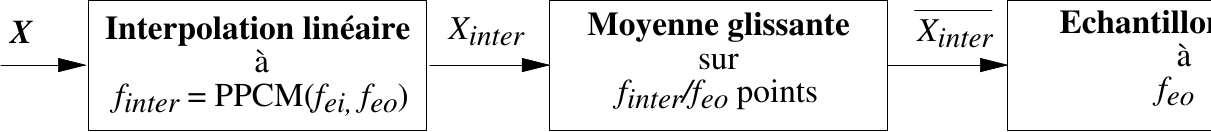
\includegraphics[width=0.8\linewidth]{images/algo_MoyEch_ff.png}
\captionof{figure}{Sch�ma fonctionnel de \operfmt{MoyEch\_ff}}
\label{fig:algo_MoyEch_ff}
}

%%%%%AUTEUR%%%%
\itemstyle{Auteur~:}
CNRM/GMEI/TRAMM

%%%%%REFERENCE%%%%
\itemstyle{R�f�rences~:}

\newpage
%%%%%
%
\section{Moyenne-Echantillonnage 
 en tol�rant des valeurs manquantes (param\`etre \texttt{float})}

\itemstyle{Op\'erateur~:} \operfmt{MoyEch\_mnq}
\label{OP-MoyEch_mnq}
\index{MoyEch\_mnq}

%%%%%OBJET%%%%
\itemstyle{Objet~:}
Moyenne glissante et \'echantillonnage d'un
param\`etre \`a une fr\'equence donn\'ee, diviseur
de la fr\'equence du param\`etre d'entr\'ee.
Le calcul tient compte de la pr�sence des valeurs manquantes
et permet � l'utilisateur de choisir la tol�rance en terme 
de nombre de valeurs manquantes.

%%%%%ARGUMENTS%%%%
\bigskip
%%%%%ENTREES%%%%
\begin{tabarg}
\multicolumn{3}{l}{\titretab {Entr\'ees}}\\
\hline
$X$ & Vecteur, \texttt{float} & Param\`etre d'entr\'ee\\
$R_f$ & Coeff., \texttt{double} & Rapport des fr\'equences $ \frac{F_{sortie}}
{F_{entree}}$, dans l'intervalle $]0, 1]$\\
$Decal$ & Coeff., \texttt{int} & D\'ecalage (\textit{nombre d'�chantillons}),
 dans l'intervalle $[-1/R_f, 1/R_f]$ \\
$Toler\_{mnq}$ & Coeff., \texttt{int} & Tol\'erance pour les valeurs manquantes
 (\textit{nombre d'�chantillons})\\
\end{tabarg}

\medskip
%%%%%SORTIES%%%%
\begin{tabarg}
\multicolumn{3}{l}{\titretab {Sorties}}\\
\hline
$X_m$ & Vecteur, \texttt{float} & Moyennes (m\^eme unit\'e que $X$)\\
\end{tabarg}


%%%%%FORMULE%%%%
\itemstyle{Formule}

%%Moy
\[
Xm[i] = R_f . \sum_{j = i/R_f + Decal}^{(i+1)/R_f -1 + Decal} X[j]
\qquad i=0,Nbre\_Echant(X). R_f
\]


%%%%COMMENTAIRE%%%%
\itemstyle{Commentaire~:}

$R_f$ doit \^etre l'inverse d'un entier. Si ce n'est pas le cas, utiliser
\hyperref[OP-MoyEch_ff]{\operfmt{MoyEch\_ff}}.  \newline
Le nombre d'\'echantillons du vecteur de sortie est le produit du
nombre d'\'echantillons du vecteur d'entr\'ee par $R_f$, arrondi
\`a l'entier sup\'erieur. \newline

%%%%%AUTEUR%%%%
\itemstyle{Auteur~:}
CNRM/GMEI/TRAMM

%%%%%REFERENCE%%%%
\itemstyle{R\'ef\'erences~:}

\newpage
%%%%%
%
\section{Moyenne-Echantillonnage 
 en tol�rant des valeurs manquantes (param\`etre {\tt short})}

\itemstyle{Op\'erateur~:} \operfmt{ MoyEch\_mnq\_int}
\index{MoyEch\_mnq\_int}

%%%%%OBJET%%%%
\itemstyle{Objet~:}
Moyenne glissante et \'echantillonnage d'un
param\`etre \`a une fr\'equence donn\'ee, diviseur
de la fr\'equence du param\`etre d'entr\'ee.
Le calcul tient compte de la pr�sence des valeurs manquantes
et permet � l'utilisateur de choisir la tol�rance en terme 
de nombre de valeurs manquantes.
Le r�sultat est un param\`etre r\'eel arrondi \`a la valeur
enti\`ere la plus proche. 

%%%%%ARGUMENTS%%%%
\bigskip
%%%%%ENTREES%%%%
\begin{tabarg}
\multicolumn{3}{l}{\titretab {Entr\'ees}}\\
\hline
$X$ & Vecteur, \texttt{short} & Param\`etre d'entr\'ee\\
$R_f$ & Coeff., \texttt{double} & Rapport des fr\'equences $ F_{sortie}\over
F_{entree}$ , dans l'intervalle $]0, 1]$\\
$Decal$ & Coeff., \texttt{int} & D\'ecalage (\textit{nombre de points}), dans l'intervalle $[-1/R_f, 1/R_f]$\\
$Toler\_mnq$ & Coeff., \texttt{int} & Tolerance pour les valeurs manquantes (\textit{nombre de points}),
 entre $0$ et $1/R_f$\\
\end{tabarg}

\medskip
%%%%%SORTIES%%%%
\begin{tabarg}
\multicolumn{3}{l}{\titretab {Sorties}}\\
\hline
$X_m$ & Vecteur, \texttt{float} & R\'esultat nombre entier (m\^eme unit\'e que $X$)\\
\end{tabarg}


%%%%%FORMULE%%%%
\itemstyle{Formule}

%%Moy
$$
Xm[i] = R_f . \sum_{j = i/R_f + Decal}^{(i+1)/R_f -1 + Decal} X[j]
\qquad i=0,Nbre\_Echant(X). R_f
$$


%%%%COMMENTAIRE%%%%
\itemstyle{Commentaire~:}

$R_f$ doit \^etre l'inverse d'un entier. \newline
Le nombre d'\'echantillons du vecteur de sortie est le produit du
nombre d'\'echantillons du vecteur d'entr\'ee par $R_f$, arrondi
\`a l'entier sup\'erieur. \newline

%%%%%AUTEUR%%%%
\itemstyle{Auteur~:}
CNRM/GMEI/TRAMM

%%%%%REFERENCE%%%%
\itemstyle{R\'ef\'erences~:}

\newpage
%%%%%
%
\section{Moyenne-Echantillonnage 
 en tol�rant des valeurs manquantes (param\`etre {\tt double})}

\itemstyle{Op\'erateur~:} \operfmt{ MoyEch\_mnq\_dbl}
\index{MoyEch\_mnq\_dbl}

%%%%%OBJET%%%%
\itemstyle{Objet~:}
Moyenne glissante et \'echantillonnage d'un
param\`etre \`a une fr\'equence donn\'ee, diviseur
de la fr\'equence du param\`etre d'entr\'ee.
Le calcul tient compte de la pr�sence des valeurs manquantes
et permet � l'utilisateur de choisir la tol�rance en terme 
de nombre de valeurs manquantes.

%%%%%ARGUMENTS%%%%
\bigskip
%%%%%ENTREES%%%%
\begin{tabarg}
\multicolumn{3}{l}{\titretab {Entr\'ees}}\\
\hline
$X$ & Vecteur, \texttt{double} & Param\`etre d'entr\'ee\\
$R_f$ & Coeff., \texttt{double} & Rapport des fr\'equences $ F_{sortie}\over
F_{entree} $, dans l'intervalle $]0, 1]$\\
$Decal$ & Coeff., \texttt{int} & D\'ecalage (\textit{nombre de points}), dans 
l'intervalle $[-1/R_f, 1/R_f]$\\
$Toler\_mnq$ & Coeff., \texttt{int} & Tolerance pour les valeurs manquantes (\textit{nombre de points}),
entre $0$ et $1/R_f$\\
\end{tabarg}

\medskip
%%%%%SORTIES%%%%
\begin{tabarg}
\multicolumn{3}{l}{\titretab {Sorties}}\\
\hline
$X_m$ & Vecteur, \texttt{double} & R\'esultat (m\^eme unit\'e que $X$)\\
\end{tabarg}


%%%%%FORMULE%%%%
\itemstyle{Formule}

%%Moy
$$
Xm[i] = R_f . \sum_{j = i/R_f + Decal}^{(i+1)/R_f -1 + Decal} X[j]
\qquad i=0,Nbre\_Echant(X). R_f
$$


%%%%COMMENTAIRE%%%%
\itemstyle{Commentaire~:}

$R_f$ doit \^etre l'inverse d'un entier. \newline
Le nombre d'\'echantillons du vecteur de sortie est le produit du
nombre d'\'echantillons du vecteur d'entr\'ee par $R_f$, arrondi
\`a l'entier sup\'erieur. \newline

%%%%%AUTEUR%%%%
\itemstyle{Auteur~:}
CNRM/GMEI/TRAMM

%%%%%REFERENCE%%%%
\itemstyle{R\'ef\'erences~:}

\newpage
%%%%%
%
\section{�chantillonnage (et moyenne) d'une variable sur une nouvelle base
de temps}

\itemstyle{Op\'erateur~:} \textsf{MoyEch\_tps\_impos}
\index{MoyEch\_tps\_impos}

%%%%%OBJET%%%%
\itemstyle{Objet~:}
Cette fonction calcule, pour chaque instant $t$ d'une
base de temps "time\_out", 
une variable "X\_out", contenant la moyenne des
valeurs de  "X\_in" entre $t$-�cart\_avant et $t$+�cart\_apr�s.

Aucune supposition n'est faite sur la r�gularit� de
l'�chantillonnage des 2 variables. Cette fonction peut
donc servir, par exemple, � transformer une s�rie temporelle
asynchrone en une s�rie r�guli�re. Il est cependant n�cessaire
que time\_in (le temps de X\_in) soit "� peu pr�s" tri� par ordre
croissant.


%%%%%ARGUMENTS%%%%
\bigskip
%%%%%ENTREES%%%%
\begin{tabarg}
\multicolumn{3}{l}{\titretab {Entr\'ees}}\\
\hline
$X_{in}$ & Vecteur, \texttt{float} & Variable d'origine\\
$time_{in}$ & Vecteur, \texttt{double} & Base de temps de $X_{in}$ (secondes)\\
$ecart\_avant$ & Coeff., \texttt{double} & �cart maxi avant (secondes)\\
$ecart\_apres$ & Coeff., \texttt{double} & �cart maxi apr�s (secondes)\\
$toler\_mnq$ & Coeff., \texttt{Int\_32} & Seuil de calcul de la moyenne (nb. �chant). A chaque instant de la base de temps d'arriv�e, 
la moyenne est calcul�e si le nombre d'�chantillons dans l'intervalle de temps est strictement sup�rieur � $toler\_mnq$. Sinon, 
le r�sultat est "valeur manquante". Une valeur de 0 provoque le calcul dans tous les cas (m�me s'il n'y a qu'un seul �chantillon).\\
$time_{out}$ & Vecteur, \texttt{double} & Base de temps d'arriv�e (secondes)\\
$size_{out}$ & Coeff., \texttt{Int\_32} & Nombre de valeurs dans la base de temps 
d'arriv�e (dans adc, utiliser \$Arg6.NbVal)\\
\end{tabarg}

\medskip
%%%%%SORTIES%%%%
\begin{tabarg}
\multicolumn{3}{l}{\titretab {Sorties}}\\
\hline
$X_{out}$ & Vecteur, \texttt{float} & $X_{in}$ moyenn� et �chantillonn� sur
la base de $time_{out}$ (m�me unit� que $X_{in})$\\
\end{tabarg}


%%%%%FORMULE%%%%
\itemstyle{Formule}

%% MoyEch_tps_impos
\[
X_{out}[i] = \frac{
\displaystyle{\sum_{t[i] - ecart\_avant}^{t[i] + ecart\_apres} X_{in}[j]} }
{N} 
\qquad i=0,Nbre\_Echant(time_{out})
\]



%%%%%AUTEUR%%%%
\itemstyle{Auteur~:}
CNRM/GMEI/TRAMM

%%%%%REFERENCE%%%%
\itemstyle{R\'ef\'erences~:}
N�ant.

\newpage
%%%%%
%
%% Dans ce fichier, les �ventuels accents sont cod�s
%% en ISO-8859-15 (aka latin9)
%% La ligne suivante donne trois exemples 
%% e accent aigu : �, e accent grave : �, e-dans-l'o : �
\section{�chantillonnage (et moyenne) d'une variable \texttt{double} sur une nouvelle base
de temps}

\itemstyle{Op�rateur~:} \operfmt{MoyEch\_tps\_impos\_dbl}
\index{MoyEch\_tps\_impos\_dbl}

%%%%%OBJET%%%%
\itemstyle{Objet~:}
Cette fonction calcule, pour chaque instant $t$ d'une
base de temps "time\_out", 
une variable "X\_out", contenant la moyenne des
valeurs de  "X\_in" entre $t$-�cart\_avant et $t$+�cart\_apr�s.

Aucune supposition n'est faite sur la r�gularit� de
l'�chantillonnage des 2 variables. Cette fonction peut
donc servir, par exemple, � transformer une s�rie temporelle
asynchrone en une s�rie r�guli�re. Il est cependant n�cessaire
que time\_in (le temps de X\_in) soit "� peu pr�s" tri� par ordre
croissant.

%%%%%ARGUMENTS%%%%
\bigskip
%% Dans ce fichier, les �ventuels accents sont cod�s
%% en ISO-8859-15 (aka latin9)
%% La ligne suivante donne trois exemples 
%% e accent aigu : �, e accent grave : �, e-dans-l'o : �
%%%%%ENTREES%%%%
\begin{tabarg}
\multicolumn{3}{l}{\titretab {Entr\'ees}}\\
\hline
$X_{in}$ & Vecteur, \texttt{double} & Variable d'origine\\
$time_{in}$ & Vecteur, \texttt{double} & Base de temps de $X_{in}$ (secondes)\\
$ecart\_avant$ & Coeff., \texttt{double} & �cart maxi avant (secondes)\\
$ecart\_apres$ & Coeff., \texttt{double} & �cart maxi apr�s (secondes)\\
$toler\_mnq$ & Coeff., \texttt{Int\_32} & Seuil de calcul de la moyenne (nb. �chant). A chaque instant de la base de temps d'arriv�e, 
la moyenne est calcul�e si le nombre d'�chantillons dans l'intervalle de temps est strictement sup�rieur � $toler\_mnq$. Sinon, 
le r�sultat est "valeur manquante". Une valeur de 0 provoque le calcul dans tous les cas (m�me s'il n'y a qu'un seul �chantillon).\\
$time_{out}$ & Vecteur, \texttt{double} & Base de temps d'arriv�e (secondes)\\
$size_{out}$ & Coeff., \texttt{Int\_32} & Nombre de valeurs dans la base de temps 
d'arriv�e (dans adc, utiliser \$Arg6.NbVal)\\
\end{tabarg}

\medskip
%%%%%SORTIES%%%%
\begin{tabarg}
\multicolumn{3}{l}{\titretab {Sorties}}\\
\hline
$X_{out}$ & Vecteur, \texttt{double} & $X_{in}$ moyenn� et �chantillonn� sur
la base de $time_{out}$ (m�me unit� que $X_{in})$\\
\end{tabarg}


%%%%%FORMULE%%%%
\itemstyle{Formule}

%% Formule de l'operateur : MoyEch_tps_impos_dbl
%% Dans ce fichier, les �ventuels accents sont cod�s
%% en ISO-8859-15 (aka latin9)
%% La ligne suivante donne trois exemples 
%% e accent aigu : �, e accent grave : �, e-dans-l'o : �
\[
X_{out}[i] = \frac{
\displaystyle{\sum_{t[i] - ecart\_avant}^{t[i] + ecart\_apres} X_{in}[j]} }
{N} 
\qquad i=0,Nbre\_Echant(time_{out})
\]


%%%%%AUTEUR%%%%
\itemstyle{Auteur~:}
CNRM/GMEI/TRAMM

%%%%%REFERENCE%%%%
\itemstyle{R�f�rences~:}

\newpage
%%%%%
%
\section{�chantillonnage et moyenne d'une variable sur une nouvelle base
de temps donn�e par un time\_{bnds}}

\itemstyle{Op\'erateur~:} \textsf{MoyEch\_tps\_{bnds}}
\index{MoyEch\_tps\_bnds}

%%%%%OBJET%%%%
\itemstyle{Objet~:}
Cette fonction calcule, pour chaque instant $t$ d'une
base de temps $time_{out}$, 
une variable $X_{out}$, contenant la moyenne des
valeurs de  $X_{in}$ entre les bornes donn�es par le $time_{bnds}$ associ� � $time_{out}$.

Aucune supposition n'est faite sur la r�gularit� de
l'�chantillonnage des 2 variables. Cette fonction peut
donc servir, par exemple, � transformer une s�rie temporelle
asynchrone en une s�rie r�guli�re. Il est cependant n�cessaire
que $time_{in}$ (le temps de $X_{in}$) soit "� peu pr�s" tri� par ordre
croissant.


%%%%%ARGUMENTS%%%%
\bigskip
%%%%%ENTREES%%%%
\begin{tabarg}
\multicolumn{3}{l}{\titretab {Entr\'ees}}\\
\hline
$X_{in}$ & Vecteur, \texttt{float} & Variable d'origine\\
$toler_{mnq}$ & Coeff., \texttt{Int\_32} & Seuil de calcul de la moyenne (nb. �chant). A chaque instant de la base de temps d'arriv�e, 
la moyenne est calcul�e si le nombre d'�chantillons dans l'intervalle de temps est strictement sup�rieur � $toler_{mnq}$. Sinon,le r�sultat est "valeur manquante". Si $toler_{mnq}$ = 0, le calcul est fait d�s qu'il y a au moins une valeur valide dans l'�chantillon. \\
$time_{out}$ & Vecteur, \texttt{double} & Base de temps d'arriv�e (secondes)\\
\end{tabarg}

\medskip
%%%%%SORTIES%%%%
\begin{tabarg}
\multicolumn{3}{l}{\titretab {Sorties}}\\
\hline
$X_{out}$ & Vecteur, \texttt{float} & $X_{in}$ moyenn� et �chantillonn� sur
la base de $time_{out}$ (m�me unit� que $X_{in})$\\
\end{tabarg}



%%%%%FORMULE%%%%
\itemstyle{Formule}

%% MoyEch_tps_bnds
Pour  i=$0$, Nbre $Time_{bnds}$ :
\[
X_{out}[i] = \frac{
\displaystyle{\sum_{tb[i][0]}^{tb[i][1]} X_{in}[j]} }
{N_{i}} 
\]
 
Pour chaque $X_{in}[j]$ diff\'{e}rent de NaN avec $N_i$ le nombre de donn\'ees dans l'intervalle tb  diff\'erent de NaN.


%%%%COMMENTAIRE%%%%
\itemstyle{Commentaire~:}
\textit{tb} est un tableau d'intervalles de temps d�termin�s � partir du vecteur temps $time_{out}$.
Cet op�rateur prend en compte des vecteurs 1D et 2D.

%%%%%AUTEUR%%%%
\itemstyle{Auteur~:}
CNRM/GMEI/TRAMM

%%%%%REFERENCE%%%%
\itemstyle{R\'ef\'erences~:}
N�ant.

\newpage
%%%%%
%
\section{�chantillonnage et moyenne d'une variable sur une nouvelle base
de temps donn�e par un time\_{bnds} en tenant compte de valeurs invalides}

\itemstyle{Op\'erateur~:} \operfmt{MoyInvEch\_tps\_{bnds}}
\index{MoyInvEch\_tps\_bnds}

%%%%%OBJET%%%%
\itemstyle{Objet~:}
Cette fonction calcule, pour chaque instant $t$ d'une
base de temps $time_{out}$, 
une variable $X_{out}$, contenant la moyenne des
valeurs de  $X_{in}$ entre les bornes donn�es par le $time_{bnds}$ associ� � $time_{out}$.
Le calcul n'est r�alis� que pour des valeurs < $val_{inv}$.
Aucune supposition n'est faite sur la r�gularit� de
l'�chantillonnage des 2 variables. Cette fonction peut
donc servir, par exemple, � transformer une s�rie temporelle
asynchrone en une s�rie r�guli�re. Il est cependant n�cessaire
que $time_{in}$ (le temps de $X_{in}$) soit "� peu pr�s" tri� par ordre
croissant.


%%%%%ARGUMENTS%%%%
\bigskip
%% Dans ce fichier, les �ventuels accents sont cod�s
%% en ISO-8859-15 (aka latin9)
%% La ligne suivante donne trois exemples 
%% e accent aigu : �, e accent grave : �, e-dans-l'o : �
%%%%%ENTREES%%%%
\begin{tabarg}
\multicolumn{3}{l}{\titretab {Entr\'ees}}\\
\hline
$X_{in}$ & Vecteur, \texttt{float} & Variable d'origine\\
$toler_{mnq}$ & Coeff., \texttt{Int\_32} & Seuil de calcul de la moyenne (nb. �chant). A chaque instant de la base de temps d'arriv�e, 
la moyenne est calcul�e si le nombre d'�chantillons dans l'intervalle de temps est strictement sup�rieur � $toler_{mnq}$. Sinon, 
le r�sultat est "valeur manquante". Si $toler_{mnq}$ = 0, le calcul est fait d�s qu'il y a au moins une valeur valide dans l'�chantillon. \\
$time_{out}$ & Vecteur, \texttt{double} & Base de temps d'arriv�e (secondes)\\
$val_{inv}$ & Coeff., \texttt{float} & valeur invalide pour laquelle la Moyenne n'est pas calcul�e \\
$val_{remplac}$ & Coeff., \texttt{float} & valeur de remplacement quand la valeur atteint val\_{inv} avec une tol�rance \\
$tolerance_{inv}$ & Coeff., \texttt{float} & proportion de valeurs n�cessaires pour que le calcul de la moyenne soit valide (entre 0 et 1). Si le nb de valeurs utilis�es pour calculer la moyenne divis� par le nombre de valeurs de la p�riode est < tol�rance\_{inv}, la valeur de la moyenne est mise �  val\_{remplac} \\
\end{tabarg}

\medskip
%%%%%SORTIES%%%%
\begin{tabarg}
\multicolumn{3}{l}{\titretab {Sorties}}\\
\hline
$X_{out}$ & Vecteur, \texttt{float} & $X_{in}$ moyenn� et �chantillonn� sur
la base de $time_{out}$ (m�me unit� que $X_{in})$\\
\end{tabarg}



%%%%%FORMULE%%%%
\itemstyle{Formule}

%% Formule de l'operateur : MoyInvEch_tps_bnds
%% Dans ce fichier, les �ventuels accents sont cod�s
%% en ISO-8859-15 (aka latin9)
%% La ligne suivante donne trois exemples 
%% e accent aigu : �, e accent grave : �, e-dans-l'o : �
Pour  i=$0$, Nbre  $Time_{bnds}$ :
\[
Proportion_{valid}=\frac{\texttt{nb de }X_{in} < val_{inv}}{\texttt{nb de valeur dans l'intervalle } Time\_bnds}
\]

\[
X_{out}[i] =
\begin{cases}
\begin{tabular}{ll}
$\frac{\displaystyle{\sum_{tb[i][0]}^{tb[i][1]} X_{in}[j]} }{N_i}$
&
\texttt{ si  $proportion_{valid}$ < $tolerance_{inv}$}
\\
\texttt{$val_{replac}$} & \texttt{ sinon}
\end{tabular} 
\\
\end{cases}
\]
Pour chaque $X_{in}[j]$ inf\'erieur \`a $val_{inv}$ avec $N_i$ le nombre de donn\'ees dans l'intervalle tb  pour lesquels $X_{in}[j]$ est inf\'erieur \`a $val_{inv}$ .


%%%%COMMENTAIRE%%%%
\itemstyle{Commentaire~:}
\textit{tb} est un tableau d'intervalles de temps d�termin�s � partir du vecteur temps $time_{out}$.

%%%%%AUTEUR%%%%
\itemstyle{Auteur~:}
CNRM/GMEI/TRAMM

%%%%%REFERENCE%%%%
\itemstyle{R\'ef\'erences~:}
N�ant.

\newpage
%%%%%
%
\section{�chantillonnage et moyenne harmonique d'une variable sur une nouvelle base
de temps}

\itemstyle{Op\'erateur~:} \textsf{MoyHarmEch\_tps\_impos}
\index{MoyHarmEch\_tps\_impos}

%%%%%OBJET%%%%
\itemstyle{Objet~:}
Cette fonction calcule, pour chaque instant $t$ d'une
base de temps $time_{out}$, 
une variable $X_{out}$, contenant la moyenne harmonique des
valeurs de  $X_{in}$  entre $t$-�cart\_{avant} et $t$+�cart\_{apr�s}.

Aucune supposition n'est faite sur la r�gularit� de
l'�chantillonnage des 2 variables. 
Il est cependant n�cessaire que $time_{in}$ (le temps de $X_{in}$) 
soit tri� par ordre croissant.


%%%%%ARGUMENTS%%%%
\bigskip
%%%%%ENTREES%%%%
\begin{tabarg}
\multicolumn{3}{l}{\titretab {Entr\'ees}}\\
\hline
$X_{in}$ & Vecteur, \texttt{float} & Variable d'origine\\
$time_{in}$ & Vecteur, \texttt{double} & Base de temps de $X_{in}$ (secondes)\\
$ecart\_avant$ & Coeff., \texttt{double} & �cart maxi avant (secondes)\\
$ecart\_apres$ & Coeff., \texttt{double} & �cart maxi apr�s (secondes)\\
$toler\_mnq$ & Coeff., \texttt{Int\_32} & Seuil de calcul de la moyenne (nb. �chant). A chaque instant de la base de temps d'arriv�e, 
la moyenne harmonique est calcul�e si le nombre d'�chantillons dans l'intervalle de temps est strictement sup�rieur � $toler\_mnq$. Sinon, 
le r�sultat est "valeur manquante". Une valeur de 0 provoque le calcul dans tous les cas (m�me s'il n'y a qu'un seul �chantillon).\\
$time_{out}$ & Vecteur, \texttt{double} & Base de temps d'arriv�e (secondes)\\
$size_{out}$ & Coeff., \texttt{Int\_32} & Nombre de valeurs dans la base de temps 
d'arriv�e (dans adc, utiliser \$Arg6.NbVal)\\
\end{tabarg}

\medskip
%%%%%SORTIES%%%%
\begin{tabarg}
\multicolumn{3}{l}{\titretab {Sorties}}\\
\hline
$X_{out}$ & Vecteur, \texttt{float} & $X_{in}$ moyenn� et �chantillonn� sur
la base de $time_{out}$ (m�me unit� que $X_{in})$\\
\end{tabarg}


%%%%%FORMULE%%%%
\itemstyle{Formule}

%% MoyHarmEch_tps_impos
\[
X_{out}[i] = \frac {N}{\displaystyle{\sum_{t[i] - ecart\_avant}^{t[i] + ecart\_apres} \frac{1}{X_{in}[j]} } }
\qquad i=0,Nbre\_Echant(time_{out})
\]



%%%%%AUTEUR%%%%
\itemstyle{Auteur~:}
CNRM/GMEI/TRAMM

%%%%%REFERENCE%%%%
\itemstyle{R\'ef\'erences~:}
N�ant.

\newpage
%%%%%
%
%% Dans ce fichier, les �ventuels accents sont cod�s
%% en ISO-8859-15 (aka latin9)
%% La ligne suivante donne trois exemples 
%% e accent aigu : �, e accent grave : �, e-dans-l'o : �
\section{�chantillonnage et moyenne harmonique d'une variable sur une nouvelle base
de temps donn�e par un time\_bnds}

\itemstyle{Op\'erateur~:} \operfmt{MoyHarmEch\_tps\_bnds}
\index{MoyHarmEch\_tps\_bnds}

%%%%%OBJET%%%%
\itemstyle{Objet~:}
Cette fonction calcule, pour chaque instant $t$ d'une
base de temps $time_{out}$, 
une variable $X_{out}$, contenant la moyenne harmonique des
valeurs de  $X_{in}$ entre les bornes donn�es par le $time_{bnds}$ associ� � $time_{out}$.

Aucune supposition n'est faite sur la r�gularit� de
l'�chantillonnage des 2 variables. 
Il est cependant n�cessaire que $time_{in}$ (le temps de $X_{in}$) 
soit tri� par ordre croissant.


%%%%%ARGUMENTS%%%%
\bigskip
%% Dans ce fichier, les �ventuels accents sont cod�s
%% en ISO-8859-15 (aka latin9)
%% La ligne suivante donne trois exemples 
%% e accent aigu : �, e accent grave : �, e-dans-l'o : �
%%%%%ENTREES%%%%
\begin{tabarg}
\multicolumn{3}{l}{\titretab {Entr\'ees}}\\
\hline
$X_{in}$ & Vecteur, \texttt{float} & Variable d'origine\\
$toler_{mnq}$ & Coeff., \texttt{Int\_32} & Seuil de calcul de la moyenne (nb. �chant). A chaque instant de la base de temps d'arriv�e, 
la moyenne harmonique est calcul�e si le nombre d'�chantillons dans l'intervalle de temps est strictement sup�rieur � $toler_{mnq}$. Sinon, 
le r�sultat est "valeur manquante". Si $toler_{mnq}$ = 0, le calcul est fait d�s qu'il y a au moins une valeur valide dans l'�chantillon. \\
$time_{out}$ & Vecteur, \texttt{double} & Base de temps d'arriv�e (secondes)\\
\end{tabarg}

\medskip
%%%%%SORTIES%%%%
\begin{tabarg}
\multicolumn{3}{l}{\titretab {Sorties}}\\
\hline
$X_{out}$ & Vecteur, \texttt{float} & $X_{in}$ moyenn� et �chantillonn� sur
la base de $time_{out}$ (m�me unit� que $X_{in})$\\
\end{tabarg}



%%%%%FORMULE%%%%
\itemstyle{Formule}

%% Formule de l'operateur : MoyHarmEch_tps_bnds
%% Dans ce fichier, les �ventuels accents sont cod�s
%% en ISO-8859-15 (aka latin9)
%% La ligne suivante donne trois exemples 
%% e accent aigu : �, e accent grave : �, e-dans-l'o : �
Pour  i=$0$, Nbre $Time_{bnds}$ :
\[
X_{out}[i] = \frac{N_{i}}
{\displaystyle{\sum_{tb[i][0]}^{tb[i][1]}  \frac{1}{X_{in}[j]}} }
\]
 
Pour chaque $X_{in}[j]$ diff\'{e}rent de NaN avec $N_i$ le nombre de donn\'ees dans l'intervalle tb  pour lesquels $X_{in}[j]$ est diff\'erent de NaN.


%%%%COMMENTAIRE%%%%
\itemstyle{Commentaire~:}
\textit{tb} est un tableau d'intervalles de temps d�termin�s � partir du vecteur temps $time_{out}$.

%%%%%AUTEUR%%%%
\itemstyle{Auteur~:}
CNRM/GMEI/TRAMM

%%%%%REFERENCE%%%%
\itemstyle{R\'ef\'erences~:}
N�ant.

\newpage
%%%%%
%
%% Dans ce fichier, les �ventuels accents sont cod�s
%% en ISO-8859-15 (aka latin9)
%% La ligne suivante donne trois exemples 
%% e accent aigu : �, e accent grave : �, e-dans-l'o : �
\section{�chantillonnage et moyenne harmonique d'une variable sur une nouvelle base
de temps donn�e par un time\_{bnds} en tenant compte de valeurs invalides}

\itemstyle{Op\'erateur~:} \operfmt{MoyHarmInvEch\_tps\_bnds}
\index{MoyHarmInvEch\_tps\_bnds}

%%%%%OBJET%%%%
\itemstyle{Objet~:}
Cette fonction calcule, pour chaque instant $t$ d'une
base de temps $time_{out}$, 
une variable $X_{out}$, contenant la moyenne harmonique des
valeurs de  $X_{in}$ entre les bornes donn�es par le $time_{bnds}$ associ� � $time_{out}$.
Le calcul n'est r�alis� que pour des valeurs < $val_{inv}$.
Aucune supposition n'est faite sur la r�gularit� de
l'�chantillonnage des 2 variables. Il est cependant n�cessaire
que $time_{in}$ (le temps de $X_{in}$) soit "� peu pr�s" tri� par ordre
croissant.


%%%%%ARGUMENTS%%%%
\bigskip
%% Dans ce fichier, les �ventuels accents sont cod�s
%% en ISO-8859-15 (aka latin9)
%% La ligne suivante donne trois exemples 
%% e accent aigu : �, e accent grave : �, e-dans-l'o : �
%%%%%ENTREES%%%%
\begin{tabarg}
\multicolumn{3}{l}{\titretab {Entr\'ees}}\\
\hline
$X_{in}$ & Vecteur, \texttt{float} & Variable d'origine\\
$toler_{mnq}$ & Coeff., \texttt{Int\_32} & Seuil de calcul de la moyenne harmonique(nb. �chant). A chaque instant de la base de temps d'arriv�e, 
la moyenne harmonique est calcul�e si le nombre d'�chantillons dans l'intervalle de temps est strictement sup�rieur � $toler_{mnq}$. Sinon, 
le r�sultat est "valeur manquante". Si $toler_{mnq}$ = 0, le calcul est fait d�s qu'il y a au moins une valeur valide dans l'�chantillon. \\
$time_{out}$ & Vecteur, \texttt{double} & Base de temps d'arriv�e (secondes)\\
$val_{inv}$ & Coeff., \texttt{float} & valeur invalide pour laquelle la Moyenne harmonique n'est pas calcul�e \\
$val_{remplac}$ & Coeff., \texttt{float} & valeur de remplacement quand la valeur atteint val\_{inv} %avec une tol�rance 
au moins un fois dans l'intervalle\\
\end{tabarg}

\medskip
%%%%%SORTIES%%%%
\begin{tabarg}
\multicolumn{3}{l}{\titretab {Sorties}}\\
\hline
$X_{out}$ & Vecteur, \texttt{float} & $X_{in}$ moyenn� et �chantillonn� sur
la base de $time_{out}$ (m�me unit� que $X_{in})$\\
\end{tabarg}



%%%%%FORMULE%%%%
\itemstyle{Formule}

%% Formule de l'operateur : MoyHarmInvEch_tps_bnds
%% Dans ce fichier, les �ventuels accents sont cod�s
%% en ISO-8859-15 (aka latin9)
%% La ligne suivante donne trois exemples 
%% e accent aigu : �, e accent grave : �, e-dans-l'o : �
Pour  i=$0$, Nbre  $Time_{bnds}$ :
%%%% tolerance_inv n'est pas impl�ment�e dans cet op�rateur
%\[
%Proportion_{valid}=\frac{\texttt{nb de }X_{in}[j] < %val_{inv}}{\texttt{nb de valeur dans l'intervalle } %Time\_bnds}
%\]

\[
X_{out}[i] =
\begin{cases}
\begin{tabular}{ll}
$
\frac{N_{i}}
{\displaystyle{\sum_{tb[i][0]}^{tb[i][1]} \frac{1}{X_{in}[j]}} }
$
&
\texttt{ si tous les terme de l'intervalle sont $<  val_{inv}$}
\\
\texttt{$val_{replac}$} & \texttt{ si $val_{inv}$ est atteint au moins un fois}
\end{tabular} 
\\
\end{cases}
\]

Pour chaque $X_{in}[j]$ inf\'erieur \`a $val_{inv}$ avec $N_i$ le nombre de donn\'ees dans l'intervalle tb  pour lesquels $X_{in}[j]$ est inf\'erieur \`a $val_{inv}$ .


%%%%COMMENTAIRE%%%%
\itemstyle{Commentaire~:}
\textit{tb} est un tableau d'intervalles de temps d�termin�s � partir du vecteur temps $time_{out}$.

%%%%%AUTEUR%%%%
\itemstyle{Auteur~:}
CNRM/GMEI/TRAMM

%%%%%REFERENCE%%%%
\itemstyle{R\'ef\'erences~:}
N�ant.

\newpage
%%%%%
%
\section{�chantillonnage et �cart type d'une variable sur une nouvelle base
de temps}

\itemstyle{Op\'erateur~:} \operfmt{StdMoyEch\_tps\_impos}
\index{StdMoyEch\_tps\_impos}

%%%%%OBJET%%%%
\itemstyle{Objet~:}
Cette fonction calcule, pour chaque instant $t$ d'une
base de temps "time\_out", 
une variable "X\_out", contenant l'�cart type des
valeurs de  "X\_in" entre $t$-�cart\_avant et $t$+�cart\_apr�s.

Aucune supposition n'est faite sur la r�gularit� de
l'�chantillonnage des 2 variables. Cette fonction peut
donc servir, par exemple, � transformer une s�rie temporelle
asynchrone en une s�rie r�guli�re. Il est cependant n�cessaire
que time\_in (le temps de X\_in) soit "� peu pr�s" tri� par ordre
croissant.


%%%%%ARGUMENTS%%%%
\bigskip
%% Dans ce fichier, les �ventuels accents sont cod�s
%% en ISO-8859-15 (aka latin9)
%% La ligne suivante donne trois exemples 
%% e accent aigu : �, e accent grave : �, e-dans-l'o : �
%%%%%ENTREES%%%%
\begin{tabarg}
\multicolumn{3}{l}{\titretab {Entr\'ees}}\\
\hline
$X_{in}$ & Vecteur, \texttt{float} & Variable d'origine\\
$time_{in}$ & Vecteur, \texttt{double} & Base de temps de $X_{in}$ (secondes)\\
$ecart\_avant$ & Coeff., \texttt{double} & �cart maxi avant (secondes)\\
$ecart\_apres$ & Coeff., \texttt{double} & �cart maxi apr�s (secondes)\\
$toler\_mnq$ & Coeff., \texttt{Int\_32} & Seuil de calcul de l'�cart type std(nb. �chant). A chaque instant de la base de temps d'arriv�e, 
l'�cart type est calcul� si le nombre d'�chantillons dans l'intervalle de temps est strictement sup�rieur � $toler\_mnq$. Sinon, 
le r�sultat est "valeur manquante". Une valeur de 0 provoque le calcul dans tous les cas (m�me s'il n'y a qu'un seul �chantillon).\\
$time_{out}$ & Vecteur, \texttt{double} & Base de temps d'arriv�e (secondes)\\
$size_{out}$ & Coeff., \texttt{Int\_32} & Nombre de valeurs dans la base de temps 
d'arriv�e (dans adc, utiliser \$Arg6.NbVal)\\
\end{tabarg}

\medskip
%%%%%SORTIES%%%%
\begin{tabarg}
\multicolumn{3}{l}{\titretab {Sorties}}\\
\hline
$X_{out}$ & Vecteur, \texttt{float} & $X_{in}$ moyenn� et �chantillonn� sur
la base de $time_{out}$ (m�me unit� que $X_{in})$\\
\end{tabarg}


%%%%%FORMULE%%%%
\itemstyle{Formule}

%% Formule de l'operateur : StdMoyEch_tps_impos
%% Dans ce fichier, les �ventuels accents sont cod�s
%% en ISO-8859-15 (aka latin9)
%% La ligne suivante donne trois exemples 
%% e accent aigu : �, e accent grave : �, e-dans-l'o : �
\[
X_{moy} = \frac{
\displaystyle{\sum_{t[i] - ecart\_avant}^{t[i] + ecart\_apres} X_{in}[j]} }
{N} 
\qquad i=0,Nbre\_Echant(time_{out})
\]

\[
X_{out}[i] = \frac{ \sqrt{
\displaystyle{\sum_{t[i] - ecart\_avant}^{t[i] + ecart\_apres} (X_{in}[j] - X_{moy})�} }}
{N_{i}} 
\] 
Pour chaque $X_{in}[j]$ diff\'{e}rent de NaN avec $N_i$ le nombre de donn\'ees dans l'intervalle t[i] - ecart\_avant ,  t[i] + ecart\_apres  diff\'erent de NaN.


%%%%%AUTEUR%%%%
\itemstyle{Auteur~:}
CNRM/GMEI/TRAMM

%%%%%REFERENCE%%%%
\itemstyle{R\'ef\'erences~:}
N�ant.

\newpage
%%%%%
%
\section{�chantillonnage et �cart type d'une variable sur une nouvelle base
de temps donn�e par un time\_{bnds}}

\itemstyle{Op\'erateur~:} \operfmt{StdEch\_tps\_bnds}
\index{StdEch\_tps\_bnds}

%%%%%OBJET%%%%
\itemstyle{Objet~:}
Cette fonction calcule, pour chaque instant $t$ d'une
base de temps $time_{out}$, 
une variable $X_{out}$, contenant la l'�cart type  des
valeurs de  $X_{in}$ entre les bornes donn�es par le $time_{bnds}$ associ� � $time_{out}$.

Aucune supposition n'est faite sur la r�gularit� de
l'�chantillonnage des 2 variables. Il est cependant n�cessaire
que $time_{in}$ (le temps de $X_{in}$) soit "� peu pr�s" tri� par ordre
croissant.


%%%%%ARGUMENTS%%%%
\bigskip
%% Dans ce fichier, les �ventuels accents sont cod�s
%% en ISO-8859-15 (aka latin9)
%% La ligne suivante donne trois exemples 
%% e accent aigu : �, e accent grave : �, e-dans-l'o : �
%%%%%ENTREES%%%%
\begin{tabarg}
\multicolumn{3}{l}{\titretab {Entr\'ees}}\\
\hline
$X_{in}$ & Vecteur, \texttt{float} & Variable d'origine\\
$toler_{mnq}$ & Coeff., \texttt{Int\_32} & Seuil de calcul de l'�cart type (nb. �chant). A chaque instant de la base de temps d'arriv�e, 
std est calcul� si le nombre d'�chantillons dans l'intervalle de temps est strictement sup�rieur � $toler_{mnq}$. Sinon, 
le r�sultat est "valeur manquante".. Si $toler_{mnq}$ = 0, le calcul est fait d�s qu'il y a au moins une valeur valide dans l'�chantillon. \\
$time_{out}$ & Vecteur, \texttt{double} & Base de temps d'arriv�e (secondes)\\
\end{tabarg}

\medskip
%%%%%SORTIES%%%%
\begin{tabarg}
\multicolumn{3}{l}{\titretab {Sorties}}\\
\hline
$X_{out}$ & Vecteur, \texttt{float} & Ecart type de $X_{in}$ �chantillonn� sur
la base de $time_{out}$ (m�me unit� que $X_{in})$\\
\end{tabarg}


%%%%%FORMULE%%%%
\itemstyle{Formule}

%% Formule de l'operateur : StdEch_tps_bnds
%% Dans ce fichier, les �ventuels accents sont cod�s
%% en ISO-8859-15 (aka latin9)
%% La ligne suivante donne trois exemples 
%% e accent aigu : �, e accent grave : �, e-dans-l'o : �
Pour  i=$0$, Nbre $Time_{bnds}$ :
\[
X_{moy} = \frac{
\displaystyle{\sum_{tb[i][0]}^{tb[i][1]} X_{in}[j]} }
{N_{i}} 
\]

\[
X_{out}[i] = \frac{ \sqrt{
\displaystyle{\sum_{tb[i][0]}^{tb[i][1]} (X_{in}[j] - X_{moy})�} }}
{N_{i}} 
\] 
Pour chaque $X_{in}[j]$ diff\'{e}rent de NaN avec $N_i$ le nombre de donn\'ees dans l'intervalle tb  diff\'erent de NaN.


%%%%COMMENTAIRE%%%%
\itemstyle{Commentaire~:}
\textit{tb} est un tableau d'intervalles de temps d�termin�s � partir du vecteur temps $time_{out}$.

%%%%%AUTEUR%%%%
\itemstyle{Auteur~:}
CNRM/GMEI/TRAMM

%%%%%REFERENCE%%%%
\itemstyle{R\'ef\'erences~:}

\newpage
%%%%%
%
\section{�chantillonnage et �cart type d'une variable sur une nouvelle base
de temps donn�e par un time\_{bnds} en tenant compte de valeurs invalides}

\itemstyle{Op\'erateur~:} \operfmt{StdInvEch\_tps\_bnds}
\index{StdInvEch\_tps\_bnds}

%%%%%OBJET%%%%
\itemstyle{Objet~:}
Cette fonction calcule, pour chaque instant $t$ d'une
base de temps $time_{out}$, 
une variable $X_{out}$, contenant la l'�cart type  des
valeurs de  $X_{in}$ entre les bornes donn�es par le $time_{bnds}$ associ� � $time_{out}$.
Le calcul n'est r�alis� que pour des valeurs < $val_{inv}$.
Aucune supposition n'est faite sur la r�gularit� de
l'�chantillonnage des 2 variables. Il est cependant n�cessaire
que $time_{in}$ (le temps de $X_{in}$) soit "� peu pr�s" tri� par ordre
croissant.


%%%%%ARGUMENTS%%%%
\bigskip
%% Dans ce fichier, les �ventuels accents sont cod�s
%% en ISO-8859-15 (aka latin9)
%% La ligne suivante donne trois exemples 
%% e accent aigu : �, e accent grave : �, e-dans-l'o : �
%%%%%ENTREES%%%%
\begin{tabarg}
\multicolumn{3}{l}{\titretab {Entr\'ees}}\\
\hline
$X_{in}$ & Vecteur, \texttt{float} & Variable d'origine\\
$toler_{mnq}$ & Coeff., \texttt{Int\_32} & Seuil de calcul de l'�cart type (nb. �chant). A chaque instant de la base de temps d'arriv�e, 
l'�cart type est calcul� si le nombre d'�chantillons dans l'intervalle de temps est strictement sup�rieur � $toler_{mnq}$. Sinon, 
le r�sultat est "valeur manquante". Si $toler_{mnq}$ = 0, le calcul est fait d�s qu'il y a au moins une valeur valide dans l'�chantillon. \\
$time_{out}$ & Vecteur, \texttt{double} & Base de temps d'arriv�e (secondes)\\
$val_{inv}$ & Coeff., \texttt{float} & valeur invalide pour laquelle l'�cart type n'est pas calcul� \\
$val_{remplac}$ & Coeff., \texttt{float} & valeur de remplacement quand la valeur atteint val\_{inv} avec une tol�rance \\
$tolerance_{inv}$ & Coeff., \texttt{float} & proportion de valeurs n�cessaires pour que le calcul de l'�cart type soit valide (entre 0 et 1). Si le nb de valeurs utilis�es pour calculer l'�cart type divis� par le nombre de valeurs de la p�riode est < tol�rance\_{inv}, la valeur est mise �  val\_{remplac} \\
\end{tabarg}

\medskip
%%%%%SORTIES%%%%
\begin{tabarg}
\multicolumn{3}{l}{\titretab {Sorties}}\\
\hline
$X_{out}$ & Vecteur, \texttt{float} & �cart type de $X_{in}$ �chantillonn� sur
la base de $time_{out}$ (m�me unit� que $X_{in})$\\
\end{tabarg}



%%%%%FORMULE%%%%
\itemstyle{Formule}

%% Formule de l'operateur : StdInvEch_tps_bnds
%% Dans ce fichier, les �ventuels accents sont cod�s
%% en ISO-8859-15 (aka latin9)
%% La ligne suivante donne trois exemples 
%% e accent aigu : �, e accent grave : �, e-dans-l'o : �
Pour  i=$0$, Nbre $Time_{bnds}$ :
\[
Proportion_{valid}=\frac{\texttt{nb de }X_{in} < val_{inv}}{\texttt{nb de valeur dans l'intervalle } Time\_bnds}
\]

\[
X_{moy} = \frac{
\displaystyle{\sum_{tb[i][0]}^{tb[i][1]} X_{in}[j]} }
{N_{i}} 
\]

\[
X_{out}[i] =
\begin{cases}
\begin{tabular}{ll}
$ \frac{ \sqrt{
\displaystyle{\sum_{tb[i][0]}^{tb[i][1]} (X_{in}[j] - X_{moy})�} }}{N_{i}} $
&
\texttt{ si  $proportion_{valid}$ < $tolerance_{inv}$}
\\
\texttt{$val_{replac}$} & \texttt{ sinon}
\end{tabular} 
\\
\end{cases}
\]
Pour chaque $X_{in}[j]$ inf\'erieur \`a $val_{inv}$ avec $N_i$ le nombre de donn\'ees dans l'intervalle tb  pour lesquels $X_{in}[j]$ est inf\'erieur \`a $val_{inv}$ .


%%%%COMMENTAIRE%%%%
\itemstyle{Commentaire~:}
\textit{tb} est un tableau d'intervalles de temps d�termin�s � partir du vecteur temps $time_{out}$.

%%%%%AUTEUR%%%%
\itemstyle{Auteur~:}
CNRM/GMEI/TRAMM

%%%%%REFERENCE%%%%
\itemstyle{R\'ef\'erences~:}
N�ant.

\newpage
%%%%%
%
\section{�chantillonnage (et maximum) d'une variable sur une nouvelle base
de temps}

\itemstyle{Op\'erateur~:} \operfmt{MaxEch\_tps\_impos}
\index{MaxEch\_tps\_impos}

%%%%%OBJET%%%%
\itemstyle{Objet~:}
Cette fonction calcule, pour chaque instant $t$ d'une
base de temps "time\_out", 
une variable "X\_out", contenant le maximum des
valeurs de  "X\_in" entre $t$-�cart\_avant et $t$+�cart\_apr�s.

Aucune supposition n'est faite sur la r�gularit� de
l'�chantillonnage des 2 variables. Cette fonction peut
donc servir, par exemple, � transformer une s�rie temporelle
asynchrone en une s�rie r�guli�re. Il est cependant n�cessaire
que time\_in (le temps de X\_in) soit "� peu pr�s" tri� par ordre
croissant.


%%%%%ARGUMENTS%%%%
\bigskip
%%%%%ENTREES%%%%
\begin{tabarg}
\multicolumn{3}{l}{\titretab {Entr\'ees}}\\
\hline
$X_{in}$ & Vecteur, \texttt{float} & Variable d'origine\\
$time_{in}$ & Vecteur, \texttt{double} & Base de temps de $X_{in}$ (secondes)\\
$ecart\_avant$ & Coeff., \texttt{double} & �cart maxi avant (secondes)\\
$ecart\_apres$ & Coeff., \texttt{double} & �cart maxi apr�s (secondes)\\
$toler\_mnq$ & Coeff., \texttt{Int\_32} & Seuil de calcul du maximum (nb. �chant). A chaque instant de la base de temps d'arriv�e, 
le maxmum est calcul� si le nombre d'�chantillons dans l'intervalle de temps est strictement sup�rieur � $toler\_mnq$. Sinon, 
le r�sultat est "valeur manquante". Une valeur de 0 provoque le calcul dans tous les cas (m�me s'il n'y a qu'un seul �chantillon).\\
$time_{out}$ & Vecteur, \texttt{double} & Base de temps d'arriv�e (secondes)\\
$size_{out}$ & Coeff., \texttt{Int\_32} & Nombre de valeurs dans la base de temps 
d'arriv�e (dans adc, utiliser \$Arg6.NbVal)\\
\end{tabarg}

\medskip
%%%%%SORTIES%%%%
\begin{tabarg}
\multicolumn{3}{l}{\titretab {Sorties}}\\
\hline
$X_{out}$ & Vecteur, \texttt{float} & $X_{in}$ maximum et �chantillonn� sur
la base de $time_{out}$ (m�me unit� que $X_{in})$\\
\end{tabarg}


%%%%%FORMULE%%%%
\itemstyle{Formule}

%%Min
Recherche de la valeur mixnimale dans chaque �chantillon
\[
X_m[i] = \max_{{(t[i]- ecart\_avant)} \le j< {(t[i]+ ecart\_apres)}} (X[j]) 
\]



%%%%%AUTEUR%%%%
\itemstyle{Auteur~:}
CNRM/GMEI/TRAMM

%%%%%REFERENCE%%%%
\itemstyle{R\'ef\'erences~:}
N�ant.

\newpage
%%%%%
%
\section{�chantillonnage et recherche du maximum d'une variable sur une nouvelle base
de temps donn�e par un time\_{bnds}}

\itemstyle{Op\'erateur~:} \operfmt{MaxEch\_tps\_bnds}
\index{MaxEch\_tps\_bnds}

%%%%%OBJET%%%%
\itemstyle{Objet~:}
Cette fonction calcule, pour chaque instant $t$ d'une
base de temps $time_{out}$, 
une variable $X_{out}$, contenant le maximum des
valeurs de  $X_{in}$ entre les bornes donn�es par le $time_{bnds}$ associ� � $time_{out}$.

Aucune supposition n'est faite sur la r�gularit� de
l'�chantillonnage des 2 variables. Il est cependant n�cessaire
que $time_{in}$ (le temps de $X_{in}$) soit "� peu pr�s" tri� par ordre
croissant.


%%%%%ARGUMENTS%%%%
\bigskip
%% Dans ce fichier, les �ventuels accents sont cod�s
%% en ISO-8859-15 (aka latin9)
%% La ligne suivante donne trois exemples 
%% e accent aigu : �, e accent grave : �, e-dans-l'o : �
%%%%%ENTREES%%%%
\begin{tabarg}
\multicolumn{3}{l}{\titretab {Entr\'ees}}\\
\hline
$X_{in}$ & Vecteur, \texttt{float} & Variable d'origine\\
    $toler_{mnq}$ & Coeff., \texttt{Int\_32} & Seuil de calcul du maximum (nb. �chant). A chaque instant de la base de temps d'arriv�e, 
    le maximum est calcul� si le nombre d'�chantillons dans l'intervalle de temps est strictement sup�rieur � $toler_{mnq}$. Sinon, 
le r�sultat est "valeur manquante" Si $toler_{mnq}$ = 0, le calcul est fait d�s qu'il y a au moins une valeur valide dans l'�chantillon. \\
$time_{out}$ & Vecteur, \texttt{double} & Base de temps d'arriv�e (secondes)\\
\end{tabarg}

\medskip
%%%%%SORTIES%%%%
\begin{tabarg}
\multicolumn{3}{l}{\titretab {Sorties}}\\
\hline
$X_{out}$ & Vecteur, \texttt{float} & $X_{in}$ maximum �chantillonn� sur
la base de $time_{out}$ (m�me unit� que $X_{in})$\\
\end{tabarg}



%%%%%FORMULE%%%%
\itemstyle{Formule}

%%Max
Recherche de la valeur maximale dans chaque �chantillon
\[
X_M[i] = \max_{{tb[i][0]} \le j< {tb[i][1]}} (X_{in}[j]) 
\]
 
Pour chaque $X_{in}[j]$ diff\'{e}rent de NaN.


%%%%COMMENTAIRE%%%%
\itemstyle{Commentaire~:}
\textit{tb} est un tableau d'intervalles de temps d�termin�s � partir du vecteur temps $time_{out}$.

%%%%%AUTEUR%%%%
\itemstyle{Auteur~:}
CNRM/GMEI/TRAMM

%%%%%REFERENCE%%%%
\itemstyle{R\'ef\'erences~:}
N�ant.

\newpage
%%%%%
%
\section{�chantillonnage (et minimum) d'une variable sur une nouvelle base
de temps}

\itemstyle{Op\'erateur~:} \operfmt{MinEch\_tps\_impos}
\index{MinEch\_tps\_impos}

%%%%%OBJET%%%%
\itemstyle{Objet~:}
Cette fonction calcule, pour chaque instant $t$ d'une
base de temps "time\_out", 
une variable "X\_out", contenant le minimum des
valeurs de  "X\_in" entre $t$-�cart\_avant et $t$+�cart\_apr�s.

Aucune supposition n'est faite sur la r�gularit� de
l'�chantillonnage des 2 variables. Cette fonction peut
donc servir, par exemple, � transformer une s�rie temporelle
asynchrone en une s�rie r�guli�re. Il est cependant n�cessaire
que time\_in (le temps de X\_in) soit "� peu pr�s" tri� par ordre
croissant.


%%%%%ARGUMENTS%%%%
\bigskip
%%%%%ENTREES%%%%
\begin{tabarg}
\multicolumn{3}{l}{\titretab {Entr\'ees}}\\
\hline
$X_{in}$ & Vecteur, \texttt{float} & Variable d'origine\\
$time_{in}$ & Vecteur, \texttt{double} & Base de temps de $X_{in}$ (secondes)\\
$ecart\_avant$ & Coeff., \texttt{double} & �cart maxi avant (secondes)\\
$ecart\_apres$ & Coeff., \texttt{double} & �cart maxi apr�s (secondes)\\
$toler\_mnq$ & Coeff., \texttt{Int\_32} &  Seuil de calcul du minimum (nb. �chant). A chaque instant de la base de temps d'arriv�e, 
le minimum est calcul� si le nombre d'�chantillons dans l'intervalle de temps est strictement sup�rieur � $toler\_mnq$. Sinon, 
le r�sultat est "valeur manquante". Une valeur de 0 provoque le calcul dans tous les cas (m�me s'il n'y a qu'un seul �chantillon).\\
$time_{out}$ & Vecteur, \texttt{double} & Base de temps d'arriv�e (secondes)\\
$size_{out}$ & Coeff., \texttt{Int\_32} & Nombre de valeurs dans la base de temps 
d'arriv�e (dans adc, utiliser \$Arg6.NbVal)\\
\end{tabarg}

\medskip
%%%%%SORTIES%%%%
\begin{tabarg}
\multicolumn{3}{l}{\titretab {Sorties}}\\
\hline
$X_{out}$ & Vecteur, \texttt{float} & $X_{in}$ minimun et �chantillonn� sur
la base de $time_{out}$ (m�me unit� que $X_{in})$\\
\end{tabarg}


%%%%%FORMULE%%%%
\itemstyle{Formule}

%%Min
Recherche de la valeur minimale dans chaque �chantillon
\[
X_m[i] = \min_{{(t[i]- ecart\_avant)} \le j< {(t[i]+ ecart\_apres)}} (X[j]) 
\]



%%%%%AUTEUR%%%%
\itemstyle{Auteur~:}
CNRM/GMEI/TRAMM

%%%%%REFERENCE%%%%
\itemstyle{R\'ef\'erences~:}
N�ant.

\newpage
%%%%%
%
\section{�chantillonnage et recherche du minimum d'une variable sur une nouvelle base
de temps donn�e par un time\_{bnds}}

\itemstyle{Op\'erateur~:} \operfmt{MinEch\_tps\_bnds}
\index{MinEch\_tps\_bnds}

%%%%%OBJET%%%%
\itemstyle{Objet~:}
Cette fonction calcule, pour chaque instant $t$ d'une
base de temps $time_{out}$, 
une variable $X_{out}$, contenant le minimum des
valeurs de  $X_{in}$ entre les bornes donn�es par le $time_{bnds}$ associ� � $time_{out}$.

Aucune supposition n'est faite sur la r�gularit� de
l'�chantillonnage des 2 variables.  Il est cependant n�cessaire
que $time_{in}$ (le temps de $X_{in}$) soit "� peu pr�s" tri� par ordre
croissant.


%%%%%ARGUMENTS%%%%
\bigskip
%% Dans ce fichier, les �ventuels accents sont cod�s
%% en ISO-8859-15 (aka latin9)
%% La ligne suivante donne trois exemples 
%% e accent aigu : �, e accent grave : �, e-dans-l'o : �
%%%%%ENTREES%%%%
\begin{tabarg}
\multicolumn{3}{l}{\titretab {Entr\'ees}}\\
\hline
$X_{in}$ & Vecteur, \texttt{float} & Variable d'origine\\
$toler_{mnq}$ & Coeff., \texttt{Int\_32} & Seuil de calcul du minimum (nb. �chant). A chaque instant de la base de temps d'arriv�e, 
le minimum est calcul� si le nombre d'�chantillons dans l'intervalle de temps est strictement sup�rieur � $toler_{mnq}$. Sinon, 
le r�sultat est "valeur manquante". Si $toler_{mnq}$ = 0, le calcul est fait d�s qu'il y a au moins une valeur valide dans l'�chantillon. \\
$time_{out}$ & Vecteur, \texttt{double} & Base de temps d'arriv�e (secondes)\\
\end{tabarg}

\medskip
%%%%%SORTIES%%%%
\begin{tabarg}
\multicolumn{3}{l}{\titretab {Sorties}}\\
\hline
$X_{out}$ & Vecteur, \texttt{float} & $X_{in}$ minimum �chantillonn� sur
la base de $time_{out}$ (m�me unit� que $X_{in})$\\
\end{tabarg}



%%%%%FORMULE%%%%
\itemstyle{Formule}

%%Min
Recherche de la valeur minimale dans chaque �chantillon
\[
X_m[i] = \min_{{tb[i][0]} \le j< {tb[i][1]}} (X_{in}[j]) 
\]
 
Pour chaque $X_{in}[j]$ diff\'{e}rent de NaN.


%%%%COMMENTAIRE%%%%
\itemstyle{Commentaire~:}
\textit{tb} est un tableau d'intervalles de temps d�termin�s � partir du vecteur temps $time_{out}$.

%%%%%AUTEUR%%%%
\itemstyle{Auteur~:}
CNRM/GMEI/TRAMM

%%%%%REFERENCE%%%%
\itemstyle{R\'ef\'erences~:}
N�ant.

\newpage
%%%%%
%
\section{�chantillonnage (et m�diane) d'une variable sur une nouvelle base
de temps}

\itemstyle{Op\'erateur~:} \textsf{MedEch\_tps\_impos}
\index{MedEch\_tps\_impos}

%%%%%OBJET%%%%
\itemstyle{Objet~:}
Cette fonction calcule, pour chaque instant $t$ d'une
base de temps "time\_out", 
une variable "X\_out", contenant la m�diane des
valeurs de  "X\_in" entre $t$-�cart\_avant et $t$+�cart\_apr�s.

Aucune supposition n'est faite sur la r�gularit� de
l'�chantillonnage des 2 variables.
Il est cependant n�cessaire que time\_in (le temps de X\_in) soit  tri� par ordre
croissant.


%%%%%ARGUMENTS%%%%
\bigskip
%%%%%ENTREES%%%%
\begin{tabarg}
\multicolumn{3}{l}{\titretab {Entr\'ees}}\\
\hline
$X_{in}$ & Vecteur, \texttt{float} & Variable d'origine\\
$time_{in}$ & Vecteur, \texttt{double} & Base de temps de $X_{in}$ (secondes)\\
$ecart\_avant$ & Coeff., \texttt{double} & �cart maxi avant (secondes)\\
$ecart\_apres$ & Coeff., \texttt{double} & �cart maxi apr�s (secondes)\\
$toler\_mnq$ & Coeff., \texttt{Int\_32} & Seuil de calcul de la moyenne (nb. �chant). A chaque instant de la base de temps d'arriv�e, 
la moyenne est calcul�e si le nombre d'�chantillons dans l'intervalle de temps est strictement sup�rieur � $toler\_mnq$. Sinon, 
le r�sultat est "valeur manquante". Une valeur de 0 provoque le calcul dans tous les cas (m�me s'il n'y a qu'un seul �chantillon).\\
$time_{out}$ & Vecteur, \texttt{double} & Base de temps d'arriv�e (secondes)\\
$size_{out}$ & Coeff., \texttt{Int\_32} & Nombre de valeurs dans la base de temps 
d'arriv�e (dans adc, utiliser \$Arg6.NbVal)\\
\end{tabarg}

\medskip
%%%%%SORTIES%%%%
\begin{tabarg}
\multicolumn{3}{l}{\titretab {Sorties}}\\
\hline
$X_{out}$ & Vecteur, \texttt{float} & $X_{in}$ moyenn� et �chantillonn� sur
la base de $time_{out}$ (m�me unit� que $X_{in})$\\
\end{tabarg}


%%%%%FORMULE%%%%
\itemstyle{Formule}

%% MedEch_tps_impos
$X_{out}[j]$ = Mediane[i] pour  $ time_{in}[i] - ecart\_avant \le i < time_{in}[i] + ecart\_apres$.

pour  $0 \le j < Nbre\_Echant(size_{out})$


Le tri est un tri par insertion




%%%%%AUTEUR%%%%
\itemstyle{Auteur~:}
CNRM/GMEI/TRAMM

%%%%%REFERENCE%%%%
\itemstyle{R\'ef\'erences~:}
N�ant.

\newpage
%%%%%
%
\section{�chantillonnage et percentile par rapport a val\_{seuil} d'une variable sur une nouvelle base
de temps donn�e par un time\_{bnds}}

\itemstyle{Op\'erateur~:} \operfmt{PercentileEch\_tps\_bnds}
\index{PercentileEch\_tps\_bnds}

%%%%%OBJET%%%%
\itemstyle{Objet~:}
Cette fonction calcule, pour chaque instant $t$ d'une
base de temps $time_{out}$, 
une variable $X_{out}$, contenant le percentile associ� a un vecteur 
de valeurs de  $X_{in}$ entre les bornes donn�es par le $time_{bnds}$ associ� � $time_{out}$.
Aucune supposition n'est faite sur la r�gularit� de
l'�chantillonnage des 2 variables. Il est cependant n�cessaire
que $time_{in}$ (le temps de $X_{in}$) soit "� peu pr�s" tri� par ordre
croissant.


%%%%%ARGUMENTS%%%%
\bigskip
%% Dans ce fichier, les �ventuels accents sont cod�s
%% en ISO-8859-15 (aka latin9)
%% La ligne suivante donne trois exemples 
%% e accent aigu : �, e accent grave : �, e-dans-l'o : �
%%%%%ENTREES%%%%
\begin{tabarg}
\multicolumn{3}{l}{\titretab {Entr\'ees}}\\
\hline
$X_{in}$ & Vecteur, \texttt{float} & Variable d'origine\\
$toler_{mnq}$ & Coeff., \texttt{Int\_32} & Seuil de calcul du percentile (nb d'�chantillons). A chaque instant de la base de temps d'arriv�e, 
le percentile est calcul� si le nombre d'�chantillons dans l'intervalle de temps est strictement sup�rieur � $toler_{mnq}$. Sinon, 
le r�sultat est "valeur manquante". Si $toler_{mnq}$ = 0, le calcul est fait d�s qu'il y a au moins une valeur valide dans l'�chantillon\\
$time_{out}$ & Vecteur, \texttt{double} & Base de temps d'arriv�e (secondes)\\
$val_{percentile}$ & Coeff., \texttt{float} & Percentile (en pourcentage)\\
\end{tabarg}

\medskip
%%%%%SORTIES%%%%
\begin{tabarg}
\multicolumn{3}{l}{\titretab {Sorties}}\\
\hline
$X_{out}$ & Vecteur, \texttt{float} & Percentile de $X_{in}$ �chantillonn� sur
la base de $time_{out}$ (m�me unit� que $X_{in})$\\
\end{tabarg}



%%%%%FORMULE%%%%
\itemstyle{Formule}

%% PercentileEch_tps_bnds
%Recherche du percentile pour la valeur $val_{seuil}$ dans chaque �chantillon

Pour  i=$0$, Nbre  $Time_{bnds}$ :

Pour chaque j entre ${tb[i][0]}$ et ${tb[i][1]}$ :

$X_{out}[i]$ = $X_{in}[j]$ telque $val_{seuil} \%$ des valeurs sont sup�rieures
 
Pour chaque $X_{in}[j]$ diff\'{e}rent de NaN.


%%%%COMMENTAIRE%%%%
\itemstyle{Commentaire~:}
\textit{tb} est un tableau d'intervalles de temps d�termin�s � partir du vecteur temps $time_{out}$.

%%%%%AUTEUR%%%%
\itemstyle{Auteur~:}
CNRM/GMEI/TRAMM

%%%%%REFERENCE%%%%
\itemstyle{R\'ef\'erences~:}
N�ant.

\newpage
%%%%%
%
\section{�chantillonnage et percentile par rapport a val\_{seuil} d'une variable sur une nouvelle base
de temps donn�e par un time\_{bnds} en tenant compte de valeurs invalides}

\itemstyle{Op\'erateur~:} \operfmt{PercentileInvEch\_tps\_bnds}
\index{PercentileInvEch\_tps\_bnds}

%%%%%OBJET%%%%
\itemstyle{Objet~:}
Cette fonction calcule, pour chaque instant $t$ d'une
base de temps $time_{out}$, 
une variable $X_{out}$, contenant le percentile associ� a un vecteur 
de valeurs de  $X_{in}$ entre les bornes donn�es par le $time_{bnds}$ associ� � $time_{out}$.
Le calcul n'est r�alis� que pour des valeurs < $val_{inv}$.
Aucune supposition n'est faite sur la r�gularit� de
l'�chantillonnage des 2 variables. Il est cependant n�cessaire
que $time_{in}$ (le temps de $X_{in}$) soit "� peu pr�s" tri� par ordre
croissant.


%%%%%ARGUMENTS%%%%
\bigskip
%% Dans ce fichier, les �ventuels accents sont cod�s
%% en ISO-8859-15 (aka latin9)
%% La ligne suivante donne trois exemples 
%% e accent aigu : �, e accent grave : �, e-dans-l'o : �
%%%%%ENTREES%%%%
\begin{tabarg}
\multicolumn{3}{l}{\titretab {Entr\'ees}}\\
\hline
$X_{in}$ & Vecteur, \texttt{float} & Variable d'origine\\
$toler_{mnq}$ & Coeff., \texttt{Int\_32} & Seuil de calcul du percentile (nb d'�chantillons). A chaque instant de la base de temps d'arriv�e, 
le percentile est calcul� si le nombre d'�chantillons dans l'intervalle de temps est strictement sup�rieur � $toler_{mnq}$. Sinon, 
le r�sultat est "valeur manquante". Si $toler_{mnq}$ = 0 le calcul est fait d�s qu'il y a au moins une valeur valide dans la p�riode\\
$time_{out}$ & Vecteur, \texttt{double} & Base de temps d'arriv�e (secondes)\\
$seuil$ & Coeff., \texttt{float} & Seuil du percentile (en pourcentage)\\
$val_{inv}$ & Coeff., \texttt{float} & valeur invalide pour laquelle le percentile n'est pas calcul� \\
$val_{remplac}$ & Coeff., \texttt{float} & valeur de remplacement quand la valeur atteint val\_{inv}  \\
\end{tabarg}

\medskip
%%%%%SORTIES%%%%
\begin{tabarg}
\multicolumn{3}{l}{\titretab {Sorties}}\\
\hline
$X_{out}$ & Vecteur, \texttt{float} & percentile de $X_{in}$ �chantillonn� sur
la base de $time_{out}$ (m�me unit� que $X_{in})$\\
\end{tabarg}



%%%%%FORMULE%%%%
\itemstyle{Formule}

%% PercentileEch_tps_bnds
Recherche du percentile pour la valeur $val_{seuil}$ inf�rieure a $val_{remplac}$ dans chaque �chantillon

Pour  i=$0$, Nbre  $Time_{bnds}$ :

	Pour chaque j entre ${tb[i][0]}$ et ${tb[i][1]}$ 

\[
X_{out}[i] =
\begin{cases}
\begin{tabular}{ll}
\texttt{ $X_{in}[j]$ telque $val_{seuil} \%$
 des valeurs sont sup�rieures}
&
\texttt{ si chaque $X_{in}[j]$ < $val_{inv}$}
\\
\texttt{$val_{replac}$} & \texttt{ sinon}
\end{tabular} 
\\
\end{cases}
\]


%%%%COMMENTAIRE%%%%
\itemstyle{Commentaire~:}
\textit{tb} est un tableau d'intervalles de temps d�termin�s � partir du vecteur temps $time_{out}$.

%%%%%AUTEUR%%%%
\itemstyle{Auteur~:}
CNRM/GMEI/TRAMM

%%%%%REFERENCE%%%%
\itemstyle{R\'ef\'erences~:}
N�ant.

\newpage
%%%%%
%
\section{�chantillonnage et quantile d'une variable sur une nouvelle base
de temps donn�e par un time\_{bnds} }

\itemstyle{Op\'erateur~:} \operfmt{QuantileEch\_tps\_bnds}
\index{QuantileEch\_tps\_bnds}

%%%%%OBJET%%%%
\itemstyle{Objet~:}
Cette fonction calcule, pour chaque instant $t$ d'une
base de temps $time_{out}$, 
une variable $X_{out}$, contenant le quantile associ� a un vecteur de valeur de valeurs de  $X_{in}$ entre les bornes donn�es par le $time_{bnds}$ associ� � $time_{out}$.
Aucune supposition n'est faite sur la r�gularit� de
l'�chantillonnage des 2 variables. Il est cependant n�cessaire
que $time_{in}$ (le temps de $X_{in}$) soit "� peu pr�s" tri� par ordre
croissant.


%%%%%ARGUMENTS%%%%
\bigskip
%% Dans ce fichier, les �ventuels accents sont cod�s
%% en ISO-8859-15 (aka latin9)
%% La ligne suivante donne trois exemples 
%% e accent aigu : �, e accent grave : �, e-dans-l'o : �
%%%%%ENTREES%%%%
\begin{tabarg}
\multicolumn{3}{l}{\titretab {Entr\'ees}}\\
\hline
$X_{in}$ & Vecteur, \texttt{float} & Variable d'origine\\
$toler_{mnq}$ & Coeff., \texttt{Int\_32} & Seuil de calcul du quantile (nb d'�chantillons). A chaque instant de la base de temps d'arriv�e, 
le quantile est calcul� si le nombre d'�chantillons dans l'intervalle de temps est strictement sup�rieur � $toler_{mnq}$. Sinon, 
le r�sultat est "valeur manquante". Si $toler_{mnq}$ = 0, le calcul est fait d�s qu'il y a au moins une valeur valide dans l'�chantillon. \\
$time_{out}$ & Vecteur, \texttt{double} & Base de temps d'arriv�e (secondes)\\
$val_{quantile}$ & Coeff., \texttt{float} & Quantile entre 0 et 1 \\
\end{tabarg}

\medskip
%%%%%SORTIES%%%%
\begin{tabarg}
\multicolumn{3}{l}{\titretab {Sorties}}\\
\hline
$X_{out}$ & Vecteur, \texttt{float} & Quantile de $X_{in}$ �chantillonn� sur
la base de $time_{out}$ (m�me unit� que $X_{in})$\\
\end{tabarg}



%%%%%FORMULE%%%%
\itemstyle{Formule}

%% Formule de l'operateur : QuantileEch_tps_bnds
%% Dans ce fichier, les �ventuels accents sont cod�s
%% en ISO-8859-15 (aka latin9)
%% La ligne suivante donne trois exemples 
%% e accent aigu : �, e accent grave : �, e-dans-l'o : �
%Recherche du quantile pour la valeur $val_{seuil}$ dans chaque �chantillon

Pour chaque j entre ${tb[i][0]}$ et ${tb[i][1]}$: 

$X_{out}[i]$ = valeurs $X_{in}[j]$ pour laquelle on a $val_{seuil}*100 \%$ des valeurs sup�rieures � cette valeur 
 
Pour chaque $X_{in}[j]$ diff\'{e}rent de NaN.


%%%%COMMENTAIRE%%%%
\itemstyle{Commentaire~:}
\textit{tb} est un tableau d'intervalles de temps d�termin�s � partir du vecteur temps $time_{out}$.

%%%%%AUTEUR%%%%
\itemstyle{Auteur~:}
CNRM/GMEI/TRAMM

%%%%%REFERENCE%%%%
\itemstyle{R\'ef\'erences~:}
N�ant.

\newpage
%%%%%
%
\section{�chantillonnage et recherche du pourcentage de valeurs inf�rieures � val\_{seuil} sur une nouvelle base
de temps donn�e par un time\_{bnds}}

\itemstyle{Op\'erateur~:} \operfmt{PourcentSeuilEch\_tps\_bnds}
\index{PourcentSeuilEch\_tps\_bnds}

%%%%%OBJET%%%%
\itemstyle{Objet~:}
Cette fonction calcule, pour chaque instant $t$ d'une
base de temps $time_{out}$, 
une variable $X_{out}$, contenant le pourcentage 
de valeurs de  $X_{in}$ inf�rieures � $val_{seuil}$ entre les bornes donn�es par le $time_{bnds}$ associ� � $time_{out}$.
Aucune supposition n'est faite sur la r�gularit� de
l'�chantillonnage des 2 variables. Il est cependant n�cessaire
que $time_{in}$ (le temps de $X_{in}$) soit "� peu pr�s" tri� par ordre
croissant.


%%%%%ARGUMENTS%%%%
\bigskip
%% Dans ce fichier, les �ventuels accents sont cod�s
%% en ISO-8859-15 (aka latin9)
%% La ligne suivante donne trois exemples 
%% e accent aigu : �, e accent grave : �, e-dans-l'o : �
%%%%%ENTREES%%%%
\begin{tabarg}
\multicolumn{3}{l}{\titretab {Entr\'ees}}\\
\hline
$X_{in}$ & Vecteur, \texttt{float} & Variable d'origine\\
$toler_{mnq}$ & Coeff., \texttt{Int\_32} & Seuil de calcul du pourcentage (nb d'�chantillons). A chaque instant de la base de temps d'arriv�e, 
le pourcentage est calcul� si le nombre d'�chantillons dans l'intervalle de temps est strictement sup�rieur � $toler\_mnq$. Sinon, 
le r�sultat est "valeur manquante". Si $toler\_{mnq}$ = 0 le calcul est fait d�s qu'il y a au moins une valeur valide dans l'�chantillon\\
$time_{out}$ & Vecteur, \texttt{double} & Base de temps d'arriv�e (secondes)\\
$val_{seuil}$ & Coeff., \texttt{float} & Seuil de validit� (en meme unit� que $X_{in}$ )\\
\end{tabarg}

\medskip
%%%%%SORTIES%%%%
\begin{tabarg}
\multicolumn{3}{l}{\titretab {Sorties}}\\
\hline
$X_{out}$ & Vecteur, \texttt{float} & pourcentage de $X_{in}$ �chantillonn� sur
la base de $time_{out}$ (m�me unit� que $X_{in})$\\
\end{tabarg}



%%%%%FORMULE%%%%
\itemstyle{Formule}

%% PourcentEchSeuil_tps_bnds
%Recherche du pourcentage de valeurs inf�rieures � $val_{seuil}$ dans chaque �chantillon

Pour  i=$0$, Nbre  $Time_{bnds}$ :

Pour chaque j entre $t_b[i][0]$ et $t_b[i][1]$:

%\[
%X_{out}[i]=
%\frac{\displaystyle{nb de X_{in}[j]}}{N_i}
%\]

\[
X_{out}[i]=
\frac{\texttt{nb de } X_{in}[j]}{N_i}
\]

Pour chaque $X_{in}[j]$ inf\'erieur \`a $val_{seuil}$ 
et $N_i$: nb de valeurs valides et diff�rentes de $val_{seuil}$ dans l'intervalle.


%%%%COMMENTAIRE%%%%
\itemstyle{Commentaire~:}
\textit{tb} est un tableau d'intervalles de temps d�termin�s � partir du vecteur temps $time_{out}$.

%%%%%AUTEUR%%%%
\itemstyle{Auteur~:}
CNRM/GMEI/TRAMM

%%%%%REFERENCE%%%%
\itemstyle{R\'ef\'erences~:}
N�ant.

\newpage
%%%%%
%
%% Dans ce fichier, les �ventuels accents sont cod�s
%% en ISO-8859-15 (aka latin9)
%% La ligne suivante donne trois exemples 
%% e accent aigu : �, e accent grave : �, e-dans-l'o : �
\section{Hauteur de la base des nuages moyenne des 3 couches de nuages quand le nombre de couches reste constant}

\itemstyle{Op\'erateur~:} \operfmt{HbnMoyInvEch\_tps\_bnds}
\index{HbnMoyInvEch\_tps\_bnds}

%%%%%OBJET%%%%
\itemstyle{Objet~:}
Cette fonction calcule, pour chaque instant $t$ d'une
base de temps $time_{out}$, 
la moyenne de chaque couche de hauteur de base de nuage $X_{i_{out}}$ entre les bornes donn�es par le $time_{bnds}$ associ� � $time_{out}$.
Le calcul n'est r�alis� que pour des valeurs < $val_{inv}$ et si le nombre de couches < $val_{inv}$ reste constant
Aucune supposition n'est faite sur la r�gularit� de
l'�chantillonnage des 2 variables. Il est cependant n�cessaire
que $time_{in}$ (le temps des $X_{i_{in}}$) soit "� peu pr�s" tri� par ordre
croissant.


%%%%%ARGUMENTS%%%%
\bigskip
%% Dans ce fichier, les �ventuels accents sont cod�s
%% en ISO-8859-15 (aka latin9)
%% La ligne suivante donne trois exemples 
%% e accent aigu : �, e accent grave : �, e-dans-l'o : �
%%%%%ENTREES%%%%
\begin{tabarg}
\multicolumn{3}{l}{\titretab {Entr\'ees}}\\
\hline
$X1_{in}$ & Vecteur, \texttt{float} & Hauteur de la base des nuages de la premi�re couche\\
$X2_{in}$ & Vecteur, \texttt{float} & Hauteur de la base des nuages de la deuxi�me couche\\
$X3_{in}$ & Vecteur, \texttt{float} & Hauteur de la base des nuages de la troisi�me couche\\
$toler_{mnq}$ & Coeff., \texttt{Int\_32} & Seuil de calcul de la moyenne (nb. �chant). A chaque instant de la base de temps d'arriv�e, 
la moyenne est calcul�e si le nombre d'�chantillons dans l'intervalle de temps est strictement sup�rieur � $toler_{mnq}$. Sinon, 
le r�sultat est "valeur manquante". Si $toler_{mnq}$ = 0, le calcul est fait d�s qu'il y a au moins une valeur valide dans l'�chantillon. \\
$time_{out}$ & Vecteur, \texttt{double} & Base de temps d'arriv�e (secondes)\\
$val_{inv}$ & Coeff., \texttt{float} & valeur invalide pour laquelle la Moyenne n'est pas calcul�e \\
$val_{remplac}$ & Coeff., \texttt{float} & valeur de remplacement quand la valeur atteint val\_{inv} avec une tol�rance \\
$tolerance_{inv}$ & Coeff., \texttt{float} & proportion de valeurs n�cessaires pour que le calcul de la moyenne soit valide (entre 0 et 1). Si le nb de valeurs utilis�es pour calculer la moyenne divis� par le nombre de valeurs de la p�riode est < tol�rance\_{inv}, la valeur de la moyenne est mise �  val\_{remplac} \\
\end{tabarg}

\medskip
%%%%%SORTIES%%%%
\begin{tabarg}
\multicolumn{3}{l}{\titretab {Sorties}}\\
\hline
$X1_{out}$ & Vecteur, \texttt{float} & $X1_{in}$ moyenn� et �chantillonn� sur
la base de $time_{out}$ (m�me unit� que $X1_{in})$ si le nb de couches < $val_{inv}$ reste constant\\
$X2_{out}$ & Vecteur, \texttt{float} & $X2_{in}$ moyenn� et �chantillonn� sur
la base de $time_{out}$ (m�me unit� que $X2_{in})$ si le nb de couches < $val_{inv}$ reste constant\\
$X3_{out}$ & Vecteur, \texttt{float} & $X3_{in}$ moyenn� et �chantillonn� sur
la base de $time_{out}$ (m�me unit� que $X3_{in})$ si le nb de couches < $val_{inv}$ reste constant\\
\end{tabarg}



%%%%%FORMULE%%%%
\itemstyle{Formule}

%% Formule de l'operateur : HbnMoyInvEch_tps_bnds
%% Dans ce fichier, les �ventuels accents sont cod�s
%% en ISO-8859-15 (aka latin9)
%% La ligne suivante donne trois exemples 
%% e accent aigu : �, e accent grave : �, e-dans-l'o : �

Pour chaque couche Xn:

Pour  i=$0$, Nbre  $Time_{bnds}$ :

\[
Xn_{out}[i] =
\begin{cases}
\begin{tabular}{ll}
$\frac{\displaystyle{\sum_{tb[i][0]}^{tb[i][1]} Xn_{in}[j]} }{Nn_i}$
&
\texttt{ si  nb couche inf\'erieure \`a $val_{inv}$ est constant}
\\
\texttt{$val_{replac}$} & \texttt{ sinon}
\end{tabular} 
\\
\end{cases}
\]

Avec $Xn_{in}[j]$ inf\'erieur \`a $val_{inv}$ et  $Nn_i$ le nombre de donn\'ees dans l'intervalle tb  pour lesquels $Xn_{in}[j]$ est inf\'erieur \`a $val_{inv}$ .


%%%%COMMENTAIRE%%%%
\itemstyle{Commentaire~:}
\textit{tb} est un tableau d'intervalles de temps d�termin�s � partir du vecteur temps $time_{out}$.

%%%%%AUTEUR%%%%
\itemstyle{Auteur~:}
CNRM/GMEI/TRAMM

%%%%%REFERENCE%%%%
\itemstyle{R\'ef\'erences~:}
N�ant.

\newpage
%%%%%
%
%% Dans ce fichier, les �ventuels accents sont cod�s
%% en ISO-8859-15 (aka latin9)
%% La ligne suivante donne trois exemples 
%% e accent aigu : �, e accent grave : �, e-dans-l'o : �
\section{Presence d'un top de hauteur de base de nuage < a une valeur de seuil}

\itemstyle{Op\'erateur~:} \operfmt{PresenceNuageEch\_tps\_bnds}
\index{PresenceNuageEch\_tps\_bnds}

%%%%%OBJET%%%%
\itemstyle{Objet~:}
Cette fonction calcule, pour chaque instant $t$ d'une
base de temps $time_{out}$, le pourcentage de top de hauteur de base de nuage 
 inf�rieur � une valeur de seuil pour au moins une des 3 couches de hauteur de base de nuage $X_{i_{in}}$ 
entre les bornes donn�es par le $time_{bnds}$ associ� � $time_{out}$.
Aucune supposition n'est faite sur la r�gularit� de
l'�chantillonnage des 2 variables. Il est cependant n�cessaire
que $time_{in}$ (le temps des $X_{i_{in}}$) soit "� peu pr�s" tri� par ordre
croissant.


%%%%%ARGUMENTS%%%%
\bigskip
%% Dans ce fichier, les �ventuels accents sont cod�s
%% en ISO-8859-15 (aka latin9)
%% La ligne suivante donne trois exemples 
%% e accent aigu : �, e accent grave : �, e-dans-l'o : �
%%%%%ENTREES%%%%
\begin{tabarg}
\multicolumn{3}{l}{\titretab {Entr\'ees}}\\
\hline
$X1_{in}$ & Vecteur, \texttt{float} & Hauteur de la base des nuages de la premi�re couche\\
$X2_{in}$ & Vecteur, \texttt{float} & Hauteur de la base des nuages de la deuxi�me couche\\
$X3_{in}$ & Vecteur, \texttt{float} & Hauteur de la base des nuages de la troisi�me couche\\
$toler_{mnq}$ & Coeff., \texttt{Int\_32} & Nombre de top minimum pour faire le calcul (nb. �chant). A chaque instant de la base de temps d'arriv�e, 
le nombre de top est calcul� si le nombre d'�chantillons dans l'intervalle de temps est strictement sup�rieur � $toler_{mnq}$. Sinon, 
le r�sultat est "valeur manquante". Si $toler_{mnq}$ = 0, le calcul est fait d�s qu'il y a au moins une valeur valide dans l'�chantillon. \\
$time_{out}$ & Vecteur, \texttt{double} & Base de temps d'arriv�e (secondes)\\
$val_{inv}$ & Coeff., \texttt{float} & valeur invalide pour laquelle le nombre de top n'est pas calcul�. \\
\end{tabarg}

\medskip
%%%%%SORTIES%%%%
\begin{tabarg}
\multicolumn{3}{l}{\titretab {Sorties}}\\
\hline
$X_{out}$ & Vecteur, \texttt{float} & $X_{in}$ Pourcentage de valeurs pr�sentant au moins un top < $val_{inv}$ 
pour une des 3 hauteurs de hbn mesur�e\\
\end{tabarg}



%%%%%FORMULE%%%%
\itemstyle{Formule}

%% Formule de l'operateur : PresenceNuageEch_tps_bnds
%% Dans ce fichier, les �ventuels accents sont cod�s
%% en ISO-8859-15 (aka latin9)
%% La ligne suivante donne trois exemples 
%% e accent aigu : �, e accent grave : �, e-dans-l'o : �

Pour chaque couche Xn:

Pour  i=$0$, Nbre  $Time_{bnds}$ :

%Pour chaque j entre $t_b[i][0]$ et $t_b[i][1]$:

\[
X_{out}[i] =
\frac{\displaystyle{\sum_{tb[i][0]}^{tb[i][1]} (top < val_{inv} ) * 100} }{N_i}
\]
%\frac{\displaystyle{\sum_{tb[i][0]}^{tb[i][1]} Xn_{in}[j]} }{Nn_i}$
%$\frac{\displaystyle{\texttt{nb de }X_{in}[j]}}{N_i}$
%\frac{\displaystyle{\sum_{tb[i][0]}^{tb[i][1]} {\max_{{1}\lt i \lt {3} }(Xn_{in}[j] < val_{seuil}) }} }{Nn_i}
%\frac{\displaystyle{\sum_{tb[i][0]}^{tb[i][1]} \max_{{1}\lt i \lt {3} } \texttt{Xn\_{in}[j] < val\_{seuil}} } }{Nn_i}
\[
\texttt{Avec top = }
\begin{cases}
\begin{tabular}{ll}
\texttt{1}
&
\texttt{ si  au moins 1 $Xn_{in}[i]$ est inf\'erieure \`a $val_{inv}$ } \\
\texttt{0} & \texttt{ sinon} \\
\end{tabular} 
\end{cases}
\]
Avec $N_i$ le nombre de donn\'ees dans l'intervalle tb .


%%%%COMMENTAIRE%%%%
\itemstyle{Commentaire~:}
\textit{tb} est un tableau d'intervalles de temps d�termin�s � partir du vecteur temps $time_{out}$.

%%%%%AUTEUR%%%%
\itemstyle{Auteur~:}
CNRM/GMEI/TRAMM

%%%%%REFERENCE%%%%
\itemstyle{R\'ef\'erences~:}
N�ant.

\newpage
%%%%%
%
\section{Variance empirique glissante}

\itemstyle{Op\'erateur~:} {\sf Var\_Ech}
\index{Var\_Ech}

%%%%%OBJET%%%%
\itemstyle{Objet~:}
Calcul de la variance empirique, sur des sous-p�riodes
cons�cutives de taille fixe.
%($s^2 = \frac{{1}{n-1} \sum_{i=1}^n (x_i - m)^2$
%, avec $m = \frac{1}{n} \sum_{i=1}^n x_i$)

%%%%%ARGUMENTS%%%%
\bigskip
%%%%%ENTREES%%%%
\begin{tabarg}
\multicolumn{3}{l}{\titretab {Entr\'ees}}\\
\hline
$X$ & Vecteur, \texttt{float} & Param�tre sur lequel effectuer le calcul (unit� indiff�rente)\\
$R_f$ & Coeff., \texttt{double} & Rapport des fr\'equences ($\frac{F_{sortie}}
{F_{entree}}$)\\
$Decal$ & Coeff., \texttt{Int\_32} & D�calage (nombre d'�chantillons,
dans l'intervalle $[-1/R_f, 1/R_f]$)\\
$Toler\_{mnq}$ & Coeff., \texttt{Int\_32} & Tol�rance pour les valeurs manquantes (nombre d'�chantillons)\\
$flag$ & Coeff., \texttt{Int\_32} & r�serv� pour un usage ult�rieur (sans objet)\\
%%
\end{tabarg}

\medskip
%%%%%SORTIES%%%%
\begin{tabarg}
\multicolumn{3}{l}{\titretab {Sorties}}\\
\hline
$V_x$ & Vecteur, \texttt{float} & S�rie des variances empiriques successives 
(carr� de l'unit� de $X$)\\
\end{tabarg}


%%%%%FORMULE%%%%
\itemstyle{Formule}

%%Var_Ech
Pour  i=$0$, $Nbre\_Echant(X). R_f$ :
\[
I_i = \left\{X_j | \frac{i}{R_f} + Decal \leq j \le \frac{i+1}{R_f} -1 + Decal,
 X_j \in \mathbb{R}\right\}
\]
\[
m_i = \frac{1}{\mathrm{card}(I_i)} \sum_{I_i} X
\]
\[
V_x[i] = \frac{1}{\mathrm{card}(I_i)} \sum_{I_i} (X -m_i)^2
\]


%%%%%AUTEUR%%%%
\itemstyle{Auteur~:}
CNRM/GMEI/TRAMM

%%%%%REFERENCE%%%%
\itemstyle{R\'ef\'erences~:}


\newpage
%%%%%
%
\section{�chantillonnage (et variance) d'une variable sur une nouvelle base
de temps donn�e par un time\_bnds}

\itemstyle{Op\'erateur~:} \textsf{VarEch\_tps\_bnds}
\index{VarEch\_tps\_bnds}

%%%%%OBJET%%%%
\itemstyle{Objet~:}
Cette fonction calcule, pour chaque instant $t$ d'une
base de temps "time\_out", 
une variable "X\_out", contenant la variance des
valeurs de  "X\_in" entre les bornes donn�es par le "time\_bnds" associ� � "time\_out".

Aucune supposition n'est faite sur la r�gularit� de
l'�chantillonnage des 2 variables. Cette fonction peut
donc servir, par exemple, � transformer une s�rie temporelle
asynchrone en une s�rie r�guli�re. Il est cependant n�cessaire
que time\_in (le temps de X\_in) soit "� peu pr�s" tri� par ordre
croissant.


%%%%%ARGUMENTS%%%%
\bigskip
%%%%%ENTREES%%%%
\begin{tabarg}
\multicolumn{3}{l}{\titretab {Entr\'ees}}\\
\hline
$X_{in}$ & Vecteur, \texttt{float} & Variable d'origine\\
$toler\_mnq$ & Coeff., \texttt{Int\_32} & Seuil de calcul de la mvariance (nb. �chant). A chaque instant de la base de temps d'arriv�e, la variance est calcul�e si le nombre d'�chantillons dans l'intervalle de temps est strictement sup�rieur � $toler\_mnq$. Sinon, 
le r�sultat est "valeur manquante". Une valeur de 0 provoque le calcul dans tous les cas (m�me s'il n'y a qu'un seul �chantillon).\\
$time_{out}$ & Vecteur, \texttt{double} & Base de temps d'arriv�e (secondes)\\ 
\end{tabarg}

\medskip
%%%%%SORTIES%%%%
\begin{tabarg}
\multicolumn{3}{l}{\titretab {Sorties}}\\
\hline
$V_{x}$ & Vecteur, \texttt{float} & Variance de $X_{in}$ �chantillonn�e sur la base de $time_{out}$ (unit� de $X_{in}$ au carr�)\\
\end{tabarg}



%%%%%FORMULE%%%%
\itemstyle{Formule}

%%Var_Ech_tps_bnds
Pour  i=$0$, $Nbre\_Time\_bnds$ :
\[
I_i = \left\{X_j | tb[i][0] \leq time_{in}[j] \le tb[i][-1],
 X_j \in \mathbb{R}\right\}
\]
\[
m_i = \frac{1}{\mathrm{card}(I_i)} \sum_{I_i} X
\]
\[
V_x[i] = \frac{1}{\mathrm{card}(I_i)} \sum_{I_i} (X -m_i)^2
\]


%%%%COMMENTAIRE%%%%
\itemstyle{Commentaire~:}
\textit{tb} est un tableau d'intervalles de temps d�termin�s � partir du vecteur temps $time_{out}$.

%%%%%AUTEUR%%%%
\itemstyle{Auteur~:}
CNRM/GMEI/TRAMM

%%%%%REFERENCE%%%%
\itemstyle{R\'ef\'erences~:}
N�ant.

\newpage
%%%%%
%
\section{Maximum-Echantillonnage d'un param\`etre {\tt float}}

\itemstyle{Op\'erateur~:} {\sf MaxEch}
\index{MaxEch}

%%%%%OBJET%%%%
\itemstyle{Objet~:}
Calcul des valeurs maxi par \'echantillon d'un
param\`etre \`a une fr\'equence donn\'ee, exemple
recherche des valeurs maxi toutes les nn minutes
pour une vitesse de vent.
Le temps en sortie est le temps de la valeur maxi
trouv\'e dans l'\'echantillon

%%%%%ARGUMENTS%%%%
\bigskip
%%%%%ENTREES%%%%
\begin{tabarg}
\multicolumn{3}{l}{\titretab {Entr\'ees}}\\
\hline
$X$ & Vecteur, {\tt float} & Param\`etre d'entr\'ee\\
$Time_{in}$ & Vecteur, {\tt double} & Vecteur temps correspondant au vecteur d'entr\'ee\\
$R_f$ & Coeff., {\tt double} & Rapport des fr\'equences ($ F_{sortie}\over
F_{entree} $) \\
$Decal$ & Coeff., {\tt int} & D\'ecalage (\textit{nombre de points})\\
\end{tabarg}

\medskip
%%%%%SORTIES%%%%
\begin{tabarg}
\multicolumn{3}{l}{\titretab {Sorties}}\\
\hline
$Time_{out}$ & Vecteur, {\tt double} & Vecteur temps correspondant aux valeurs maxi\\
$X_m$ & Vecteur, {\tt float} & R\'esultat (m\^eme unit\'e que $X$)\\
\end{tabarg}


%%%%%FORMULE%%%%
\itemstyle{Formule}

%%Max
Recherche de la valeur max dans chaque �chantillon
\[
X_m[i] = \max_{i/R_f \le j< {(i+1)}/{R_f}} (X[j]) %%\qquad j=\frac{i}{R_f}, \frac{i+1}{R_f}
%%i=0,Nbre\_Echant(X). R_f
\]
pour $i$ variant de 0 � $Nbre\_Echant(X). R_f$.


%%%%COMMENTAIRE%%%%
\itemstyle{Commentaire~:}

$R_f$ doit \^etre compris dans l'intervalle $]0, 1]$,
et \^etre l'inverse d'un entier. \newline
Le nombre d'\'echantillons du vecteur de sortie est le produit du
nombre d'\'echantillons du vecteur d'entr\'ee par $R_f$, arrondi
\`a l'entier sup\'erieur.

%%

%%%%%AUTEUR%%%%
\itemstyle{Auteur~:}
CNRM/GMEI/TRAMM

%%%%%REFERENCE%%%%
\itemstyle{R\'ef\'erences~:}

\newpage
%%%%%
%
\section{Maximum-Echantillonnage type rafale d'un param\`etre {\tt float}}

\itemstyle{Op\'erateur~:} {\sf MaxEch\_raf}
\index{MaxEch\_raf}

%%%%%OBJET%%%%
\itemstyle{Objet~:}
Calcul des valeurs maxi par \'echantillon d'un
param\`etre \`a une fr\'equence donn\'ee, le temps
en sortie correspond \`a la fin de l\'echantillon
(et non au temps du maxi comme dans MaxEch)

%%%%%ARGUMENTS%%%%
\bigskip
%%%%%ENTREES%%%%
\begin{tabarg}
\multicolumn{3}{l}{\titretab {Entr\'ees}}\\
\hline
$X$ & Vecteur, {\tt float} & Param\`etre d'entr\'ee\\
$Time-in$ & Vecteur, {\tt double} & Vecteur temps correspondant au vecteur d'entr\'ee\\
$R_f$ & Coeff., {\tt double} & Rapport des fr\'equences ($ F_{sortie}\over
F_{entree} $) \\
$Decal$ & Coeff., {\tt int} & D\'ecalage (\textit{nombre de points})\\
\end{tabarg}

\medskip
%%%%%SORTIES%%%%
\begin{tabarg}
\multicolumn{3}{l}{\titretab {Sorties}}\\
\hline
$Time-out$ & Vecteur, {\tt double} & Vecteur temps correspondant a la fin de l\'echantillon\\
$X_m$ & Vecteur, {\tt float} & R\'esultat (m\^eme unit\'e que $X$)\\
\end{tabarg}


%%%%%FORMULE%%%%
\itemstyle{Formule}

%%Max
$$
Recherche de la valeur maxi dans chaque echantillon
\qquad i=0,Nbre\_Echant(X). R_f
$$


%%%%COMMENTAIRE%%%%
\itemstyle{Commentaire~:}

$R_f$ doit \^etre compris dans l'intervalle $]0, 1]$,
et \^etre l'inverse d'un entier. \newline
Le nombre d'\'echantillons du vecteur de sortie est le produit du
nombre d'\'echantillons du vecteur d'entr\'ee par $R_f$, arrondi
\`a l'entier sup\'erieur.

%%

%%%%%AUTEUR%%%%
\itemstyle{Auteur~:}
CNRM/GMEI/TRAMM

%%%%%REFERENCE%%%%
\itemstyle{R\'ef\'erences~:}

\newpage
%%%%%
%
\section{Valeurs maximum d'une s�rie temporelle {\tt float}}

\itemstyle{Op\'erateur~:} {\sf Max\_rel}
\index{Max\_rel}

%%%%%OBJET%%%%
\itemstyle{Objet~:}
Calcul des valeurs maxi (pics relatifs) d'un
param\`etre donn\'e
L'op�rateur renvoie des Nan lorsqu'il n'y a pas
de pics.

%%%%%ARGUMENTS%%%%
\bigskip
%%%%%ENTREES%%%%
\begin{tabarg}
\multicolumn{3}{l}{\titretab {Entr\'ees}}\\
\hline
$X$ & Vecteur, {\tt float} & Param\`etre d'entr\'ee\\
\end{tabarg}

\medskip
%%%%%SORTIES%%%%
\begin{tabarg}
\multicolumn{3}{l}{\titretab {Sorties}}\\
\hline
$X_{out}$ & Vecteur, {\tt float} & Ce vecteur contient en sortie les valeurs des maxi relatifs et des NAN (vecteur temps identique au vecteur $X$)\\
\end{tabarg}


%%%%%FORMULE%%%%
\itemstyle{Formule}

%%Max
Recherche des valeurs maxi relatives (pics) par une boucle permettant d'isoler 
les points o� la pente de la courbe change de signe


%%%%COMMENTAIRE%%%%
\itemstyle{Commentaire~:}

%%

%%%%%AUTEUR%%%%
\itemstyle{Auteur~:}
CNRM/GMEI/TRAMM

%%%%%REFERENCE%%%%
\itemstyle{R\'ef\'erences~:}

\newpage
%%%%%
%
\section{Valeurs maximum relatives d'une s�rie temporelle {\tt float}}

\itemstyle{Op\'erateur~:} {\sf Max\_rel\_histo}
\index{Max\_rel\_histo}

%%%%%OBJET%%%%
\itemstyle{Objet~:}
Calcul des valeurs maxi (pics relatifs) d'un
param\`etre donn\'e. Cet op�rateur est une variante
de l'op�rateur Max\_rel. Max\_rel renvoie des Nan lorsqu'il n'y a pas
de pics. Max\_rel\_histo renvoie la valeur maximum relative jusqu'� la suivante (histogramme en sortie).

%%%%%ARGUMENTS%%%%
\bigskip
%%%%%ENTREES%%%%
\begin{tabarg}
\multicolumn{3}{l}{\titretab {Entr\'ees}}\\
\hline
$X$ & Vecteur, {\tt float} & Param\`etre d'entr\'ee\\
\end{tabarg}

\medskip
%%%%%SORTIES%%%%
\begin{tabarg}
\multicolumn{3}{l}{\titretab {Sorties}}\\
\hline
$X_{out}$ & Vecteur, {\tt float} & Ce vecteur contient en sortie les valeurs des maxi relatifs (vecteur temps identique au vecteur $X$)\\
\end{tabarg}


%%%%%FORMULE%%%%
\itemstyle{Formule}

%%Max
Recherche des valeurs maxi relatives (pics) par une boucle permettant d'isoler 
les points o� la pente de la courbe change de signe


%%%%COMMENTAIRE%%%%
\itemstyle{Commentaire~:}

%%

%%%%%AUTEUR%%%%
\itemstyle{Auteur~:}
CNRM/GMEI/TRAMM

%%%%%REFERENCE%%%%
\itemstyle{R\'ef\'erences~:}

\newpage
%%%%%
%
\section{Interpolation lin\'eaire d'un param\`etre {\tt float}}

\itemstyle{Op\'erateur~:} {\sf Inter}
\index{Inter}

%%%%%OBJET%%%%
\itemstyle{Objet~:}
Sur-�chantillonnage par interpolation lin\'eaire \`a une fr\'equence
sup\'erieure multiple de la fr\'equence du 
param\`etre d'entr\'ee.

%%%%%ARGUMENTS%%%%
\bigskip
%%%%%ENTREES%%%%
\begin{tabarg}
\multicolumn{3}{l}{\titretab {Entr\'ees}}\\
\hline
$X$ & Vecteur, {\tt float} & Param\`etre d'entr\'ee\\
$R_f$ & Coeff., {\tt Int} & Rapport des fr\'equences ($ F_{sortie}\over
F_{entree}$ ) \\
$Decal$ & Coeff., {\tt Int} & D\'ecalage (\textit{nombre de points})\\
\end{tabarg}

\medskip
%%%%%SORTIES%%%%
\begin{tabarg}
\multicolumn{3}{l}{\titretab {Sorties}}\\
\hline
$X_I$ & Vecteur, {\tt float} & Param\`etre interpol\'e (m\^eme unit\'e que
$X$)\\
\end{tabarg}


%%%%%FORMULE%%%%
\itemstyle{Formule}

%%Inter
Interpolation lin\'eaire \`a intervalles r\'eguliers
entre 2 points du  param\`etre d'entr\'ee.
%\[
%\]


%%%% COMMENTAIRE

\itemstyle{Commentaire~:}

$R_f$ doit �tre sup�rieur ou �gal � 1, et le nombre d'\'echantillons du
vecteur de sortie est le produit du
nombre d'\'echantillons du vecteur d'entr\'ee par $R_f$.


%%%%%AUTEUR%%%%
\itemstyle{Auteur~:}
CNRM/GMEI/TRAMM

%%%%%REFERENCE%%%%
\itemstyle{R\'ef\'erences~:}

\newpage
%%%%%
%
\section{Interpolation lin\'eaire d'un param\`etre {\tt double}}

\itemstyle{Op\'erateur~:} {\sf Inter\_dbl}
\index{Inter\_dbl}

%%%%%OBJET%%%%
\itemstyle{Objet~:}
Interpolation lin\'eaire \`a une fr\'equence
sup\'erieure multiple de la fr\'equence du 
param\`etre d'entr\'ee.

%%%%%ARGUMENTS%%%%
\bigskip
%%%%%ENTREES%%%%
\begin{tabarg}
\multicolumn{3}{l}{\titretab {Entr\'ees}}\\
\hline
$X$ & Vecteur, {\tt double} & Param\`etre d'entr\'ee \\
$R_f$ & Coeff., {\tt Int} & Rapport des fr\'equences ($ F_{sortie}\over
F_{entree}$ )\\
$Decal$ & Coeff., {\tt Int} & D\'ecalage (\textit{nombre de points})\\
\end{tabarg}

\medskip
%%%%%SORTIES%%%%
\begin{tabarg}
\multicolumn{3}{l}{\titretab {Sorties}}\\
\hline
$X_I$ & Vecteur, {\tt double} & Param\`etre interpol\'e\\
\end{tabarg}


%%%%%FORMULE%%%%
\itemstyle{Formule}

%%Inter_dbl
Interpolation lin\'eaire \`a intervalle r\'eguliers
entre 2 points du  param\`etre d'entr\'ee.
%\[
%\]


%%%% COMMENTAIRE

\itemstyle{Commentaire~:}

Le nombre d'\'echantillons du vecteur de sortie est le produit du
nombre d'\'echantillons du vecteur d'entr\'ee par $R_f$.


%%%%%AUTEUR%%%%
\itemstyle{Auteur~:}
CNRM/GMEI/TRAMM

%%%%%REFERENCE%%%%
\itemstyle{R\'ef\'erences~:}

\newpage
%%%%%
%
\section{Interpolation lin\'eaire d'angle}

\itemstyle{Op\'erateur~:} \textsf{Inter\_Angl}
\index{Inter\_Angl}

%%%%%OBJET%%%%
\itemstyle{Objet~:}
Sur-�chantillonnage par interpolation lin\'eaire d'une variable 
angulaire exprim�e en radians.

%%%%%ARGUMENTS%%%%
\bigskip
%%%%%ENTREES%%%%
\begin{tabarg}
\multicolumn{3}{l}{\titretab {Entr\'ees}}\\
\hline
$X$ & Vecteur, {\tt float} & Param\`etre angulaire ($radian$)\\
$R_f$ & Coeff., {\tt Int} &  Rapport des fr\'equences  ($F_{sortie}\over
F_{entree}$ )\\
$Decal$ & Coeff., {\tt Int} & D\'ecalage (\textit{nombre de points}) \\
\end{tabarg}

\medskip
%%%%%SORTIES%%%%
\begin{tabarg}
\multicolumn{3}{l}{\titretab {Sorties}}\\
\hline
$X_I$ & Vecteur, {\tt float} & Angle interpol\'e($radian$)\\
\end{tabarg}


%%%%%FORMULE%%%%
\itemstyle{Formule}

%%Inter_Angl

Pour chaque $X[i]$ (\'echantillon de $X$), 
on  d�finit $a$ et $b$  : 
$a=X[i]$ et $b=X[i+1]\pm 2\pi$, tel que
$|b-a| < \pi$.

puis on calcule $R_f$ valeurs
par interpolation lin\'eaire entre $a$ et $b$.



%%%%%COMMENTAIRE%%%%
\itemstyle{Commentaire~:}

$R_f$ doit �tre sup�rieur ou �gal � 1, et le nombre d'\'echantillons
du vecteur de sortie est le produit du
nombre d'\'echantillons du vecteur d'entr\'ee par $R_f$.

L'algorithme choisi fonctionne quel que soit l'intervalle de d\'efinition
de la variable d'entr\'ee ($[-\pi,\pi]$ ou $[0,2\pi]$, \ldots), mais 
peut produire des valeurs sortant de cet intervalle.

%%%%%AUTEUR%%%%
\itemstyle{Auteur~:}
CNRM/GMEI/TRAMM

%%%%%REFERENCE%%%%
\itemstyle{R\'ef\'erences~:}

\newpage
%%%%%
%
\section{D\'ecalage}

\itemstyle{Op\'erateur~:} {\sf Decale}
\index{Decale}

%%%%%OBJET%%%%
\itemstyle{Objet~:}
D\'ecalage temporel d'un param\`etre par
interpolation lin\'eaire. 

%%%%%ARGUMENTS%%%%
\bigskip
%%%%%ENTREES%%%%
\begin{tabarg}
\multicolumn{3}{l}{\titretab {Entr\'ees}}\\
\hline
$X$ & Vecteur, {\tt float} & Param\`etre d'entr\'ee \\
$fe$ & Coeff., {\tt float} & Fr\'equence d'\'echantillonnage de $X$ ($Hz$)\\
$t_0$ & Coeff., {\tt float} & D\'ecalage ($s$)\\
\end{tabarg}

\medskip
%%%%%SORTIES%%%%
\begin{tabarg}
\multicolumn{3}{l}{\titretab {Sorties}}\\
\hline
$X_d$ & Vecteur, {\tt float} & Param\`etre d\'ecal\'e (m\^eme unit\'e que $X$ 
)\\
\end{tabarg}


%%%%%FORMULE%%%%
\itemstyle{Formule}

%%Decale
\begin{eqnarray*}
I_0 & = & Partie Entiere(-t_0 . f_e ) \\
F_0 & = & Partie Decimale(-t_0 . f_e ) \\
Xd[i] & = & X[i+I_0] + F_0.\left( X[i+I_0+1] + X[i+I_0] \right) \\
\end{eqnarray*}


\itemstyle{Commentaire~:}

Si $t_0$ est multiple de la p\'eriode
d'\'echantillonnage ($1/f_e$), alors le signal
est d\'ecal\'e d'un nombre entier de points, mais il
reste le m\^eme. Dans le cas contraire, 
le signal r\'esultat est interpol\'e 
lin\'eairement. Donc,  
la partie haute-fr\'equence est att\'enu\'ee. 

%%%%%AUTEUR%%%%
\itemstyle{Auteur~:}
CNRM/GMEI/TRAMM

%%%%%REFERENCE%%%%
\itemstyle{R\'ef\'erences~:}

\newpage
%%%%%
%
\section{D\'ecalage\_flt}

\itemstyle{Op\'erateur~:} {\sf Decale\_flt}
\index{Decale\_flt}

%%%%%OBJET%%%%
\itemstyle{Objet~:}
D\'ecalage temporel d'un param\`etre de dimension>1 par
interpolation lin\'eaire. 

%%%%%ARGUMENTS%%%%
\bigskip
%%%%%ENTREES%%%%
\begin{tabarg}
\multicolumn{3}{l}{\titretab {Entr\'ees}}\\
\hline
$X$ & Vecteur, {\tt float} & Param\`etre d'entr\'ee \\

$NbCol$ & Coeff., {\tt Int\_32} & Taille de la dimension hors-temps de $X$ (nombre de
"colonnes")\\
$fe$ & Coeff., {\tt float} & Fr\'equence d'\'echantillonnage de $X$ ($Hz$)\\
$t_0$ & Coeff., {\tt float} & D\'ecalage ($s$)\\
\end{tabarg}

\medskip
%%%%%SORTIES%%%%
\begin{tabarg}
\multicolumn{3}{l}{\titretab {Sorties}}\\
\hline
$X_d$ & Vecteur, {\tt float} & Param\`etre d\'ecal\'e (m\^eme unit\'e que $X$ 
)\\
\end{tabarg}


%%%%%FORMULE%%%%
\itemstyle{Formule}

%%Decale
\begin{eqnarray*}
Pour ~chaque ~colonne : \\
I_0 & = & Partie Entiere(-t_0 . f_e ) \\
F_0 & = & Partie Decimale(-t_0 . f_e ) \\
Xd[i] & = & X[i+I_0] + F_0.\left( X[i+I_0+1] + X[i+I_0] \right) \\
\end{eqnarray*}


\itemstyle{Commentaire~:}

Si $t_0$ est multiple de la p\'eriode
d'\'echantillonnage ($1/f_e$), alors le signal
est d\'ecal\'e d'un nombre entier de points, mais il
reste le m\^eme. Dans le cas contraire, 
le signal r\'esultat est interpol\'e 
lin\'eairement. Donc,  
la partie haute-fr\'equence est att\'enu\'ee. 

%%%%%AUTEUR%%%%
\itemstyle{Auteur~:}
CNRM/GMEI/TRAMM

%%%%%REFERENCE%%%%
\itemstyle{R\'ef\'erences~:}

\newpage
%%%%%
%
\section{D\'ecalage d'un param\`etre 1D}

\itemstyle{Op\'erateur~:} {\sf Decale\_1D}
\index{Decale\_1D}

%%%%%OBJET%%%%
\itemstyle{Objet~:}
D\'ecalage temporel d'un param\`etre 1D par
interpolation lin\'eaire. 

%%%%%ARGUMENTS%%%%
\bigskip
%%%%%ENTREES%%%%
\begin{tabarg}
\multicolumn{3}{l}{\titretab {Entr\'ees}}\\
\hline
$X$ & Vecteur, {\tt Int16[D]} & Param\`etre 1D d'entr\'ee \\
$D$ & Vecteur, {\tt float} & Nombre d'\'el\'ements d'un \'echantillon de $X$ \\
$fe$ & Coeff., {\tt float} & Fr\'equence d'\'echantillonnage de $X$ ($Hz$)\\
$t_0$ & Coeff., {\tt float} & D\'ecalage ($s$)\\
\end{tabarg}

\medskip
%%%%%SORTIES%%%%
\begin{tabarg}
\multicolumn{3}{l}{\titretab {Sorties}}\\
\hline
$X_d$ & Vecteur, {\tt Int16[D]} & Param\`etre d\'ecal\'e (m\^eme unit\'e que $X$ 
)\\
\end{tabarg}


%%%%%FORMULE%%%%
\itemstyle{Formule}

%%Decale
\begin{eqnarray*}
I_0 & = & Partie Entiere(-t_0 . f_e ) \\
F_0 & = & Partie Decimale(-t_0 . f_e ) \\
Xd_k[i] & = & X_k[i+I_0] + F_0.\left( X_k[i+I_0+1] + X_k[i+I_0] \right) \\
\end{eqnarray*}


\itemstyle{Commentaire~:}

Si $t_0$ est multiple de la p\'eriode
d'\'echantillonnage ($1/f_e$), alors le signal
est d\'ecal\'e d'un nombre entier de points, mais il
reste le m\^eme. Dans le cas contraire, 
le signal r\'esultat est interpol\'e 
lin\'eairement. Donc,  
la partie haute-fr\'equence est att\'enu\'ee. 

%%%%%AUTEUR%%%%
\itemstyle{Auteur~:}
CNRM/GMEI/TRAMM

%%%%%REFERENCE%%%%
\itemstyle{R\'ef\'erences~:}

\newpage
%%%%%
%
\section{Changement vecteur temps}

\itemstyle{Op\'erateur~:}  {\sf Set\_reftime}
\index{Set\_reftime}

%%%%%OBJET%%%%
\itemstyle{Objet~:}
Changement du vecteur temps associ\'e.

%%%%%ARGUMENTS%%%%
\bigskip
%%%%%ENTREES%%%%
\begin{tabarg}
\multicolumn{3}{l}{\titretab {Entr\'ees}}\\
\hline
$X$ & Vecteur, \texttt{double} & Param\`etre d'entr\'ee\\
$time_{in}$ & Vecteur, \texttt{double} & Nouvelle base de temps (secondes)\\
$size_{out}$ & Coeff., \texttt{Int\_32} & Nombre de valeurs dans la nouvelle base
de temps (dans adc, utiliser \$Arg2.NbVal)\\
\end{tabarg}

\medskip
%%%%%SORTIES%%%%
\begin{tabarg}
\multicolumn{3}{l}{\titretab {Sorties}}\\
\hline
$Y$ & Vecteur, {\texttt float} & Vecteur de Sortie. \\
\end{tabarg}


%%%%%FORMULE%%%%
\itemstyle{Formule}

%%Set_freqech_reftime
\[
Y = X 
\]



%%%%%AUTEUR%%%%
\itemstyle{Auteur~:}
CNRM/GMEI/TRAMM

%%%%%REFERENCE%%%%
\itemstyle{R\'ef\'erences~:}

\newpage
%%%%%
%
%% Dans ce fichier, les �ventuels accents sont cod�s
%% en ISO-8859-15 (aka latin9)
%% La ligne suivante donne trois exemples 
%% e accent aigu : �, e accent grave : �, e-dans-l'o : �
\section{D�calage de franchissement de seuil par un signal}

\itemstyle{Op�rateur~:} \operfmt{decale\_creneau}
\index{decale\_creneau}

%%%%%OBJET%%%%
\itemstyle{Objet~:}
D�cale dans le temps les flancs montants ou descendants 
de cr�neaux.

%%%%%ARGUMENTS%%%%
\bigskip
%% Dans ce fichier, les �ventuels accents sont cod�s
%% en ISO-8859-15 (aka latin9)
%% La ligne suivante donne trois exemples 
%% e accent aigu : �, e accent grave : �, e-dans-l'o : �
%%%%%ENTREES%%%%
\begin{tabarg}
\multicolumn{3}{l}{\titretab {Entr\'ees}}\\
\hline
$X$ & Vecteur, \texttt{float} & Donn�e d'origine (unit� quelconque)\\
time & Vecteur, \texttt{double} & Datation de $X$ (seconde)\\
seuil & Coeff., \texttt{float} & Seuil (unit� de $X$)\\
decal\_down & Coeff., \texttt{float} & D�calage temporel � appliquer aux flancs descendants (seconde)\\
decal\_up & Coeff., \texttt{float} & D�calage temporel � appliquer aux flancs montants (seconde)\\
\end{tabarg}

\medskip
%%%%%SORTIES%%%%
\begin{tabarg}
\multicolumn{3}{l}{\titretab {Sorties}}\\
\hline
$Y$ & Vecteur, \texttt{float} & $X$ avec des franchissements de seuil d�cal�s dans le temps (unit� de $X$)\\
\end{tabarg}


%%%%%FORMULE%%%%
\itemstyle{Formule}

%% Formule de l'operateur : decale_creneau
%% Dans ce fichier, les �ventuels accents sont cod�s
%% en ISO-8859-15 (aka latin9)
%% La ligne suivante donne trois exemples 
%% e accent aigu : �, e accent grave : �, e-dans-l'o : �
A chaque instant :
\[
Y_i = 
\begin{cases}
X_i \qquad \text{ si } X_i > \text{seuil et d�lai franchissement seuil > decal\_up}\\
X_{\text{pre\_seuil}} \qquad \text{ si } X_i > \text{seuil et d�lai franchissement seuil < decal\_up}\\
X_i \qquad \text{ si } X_i < \text{seuil et d�lai franchissement seuil > decal\_down}\\
X_{\text{pre\_seuil}} \qquad \text{ si } X_i < \text{seuil et d�lai franchissement seuil < decal\_down}\\
\end{cases}
\]



%%%%%AUTEUR%%%%
\itemstyle{Auteur~:}
CNRM/GMEI/TRAMM

%%%%%REFERENCE%%%%
\itemstyle{R\'ef\'erences~:}

\newpage
%%%%%
%
%% Dans ce fichier, les �ventuels accents sont cod�s
%% en ISO-8859-15 (aka latin9)
%% La ligne suivante donne trois exemples 
%% e accent aigu : �, e accent grave : �, e-dans-l'o : �
\section{Synchronisation d'une variable sur une autre base de temps par interpolation par spline}

\itemstyle{Op\'erateur~:} \operfmt{Synchro\_spline}
\index{Synchro\_spline}

%%%%%OBJET%%%%
\itemstyle{Objet~:}
Cet op�rateur interpole par spline cubique une variable sur une autre base de temps et applique un d�calage temporel donn�.

%%%%%ARGUMENTS%%%%
\bigskip
%% Dans ce fichier, les �ventuels accents sont cod�s
%% en ISO-8859-15 (aka latin9)
%% La ligne suivante donne trois exemples 
%% e accent aigu : �, e accent grave : �, e-dans-l'o : �
%%%%%ENTREES%%%%
\begin{tabarg}
\multicolumn{3}{l}{\titretab {Entr\'ees}}\\
\hline
$X$ & Vecteur, \texttt{float} & Variable � interpoler ()\\
$Temps_{Dest}$ & Vecteur, \texttt{double} & Base de temps d'arriv�e  (s)\\
$D$ & Coeff., \texttt{float} & D�calage � appliquer � $X$ (s)\\
$Unite_X$ & Coeff., \texttt{String} & Unit� de $X$ (vaut "radians", "degres" pour un angle) \\
\end{tabarg}

\medskip
%%%%%SORTIES%%%%
\begin{tabarg}
\multicolumn{3}{l}{\titretab {Sorties}}\\
\hline
$X_{sync}$ & Vecteur, \texttt{float} & Variable interpol�e et d�cal�e (m�me unit� que $X$)\\
\end{tabarg}



%%%%%FORMULE%%%%
\itemstyle{Formule}

%% Formule de l'operateur : Synchro_spline
%% Dans ce fichier, les �ventuels accents sont cod�s
%% en ISO-8859-15 (aka latin9)
%% La ligne suivante donne trois exemples 
%% e accent aigu : �, e accent grave : �, e-dans-l'o : �

Les traitements suivants sont r�alis�s :
\begin{itemize}
\item  Dans un premier temps les valeurs pour lesquelles il y a un retour en arri�re dans la base de temps de $X$ sont supprim�es. \\
\item Puis, un d�calage temporel $D$ est appliqu� � $X$.\\
\item Enfin une interpolation par splines cubiques est faite avec la fonction Numpy  \textit{UnivariateSpline} (avec le param�tre s=0).\\
\end{itemize}

Si $Unite_X$ vaut "radians" ou "degres" alors ce sont $cos(X)$ et $sin(X)$ qui sont interpol�s. $X_{sync}$ est ensuite calcul� par l'arctangente (fonction \textit{arctan2 }de Numpy). \\

Cet op�rateur ne remplace pas  les valeurs manquantes dans $X$. C'est-�-dire, les valeurs qui sont manquantes dans $X$ sont aussi manquantes dans $X_{sync}$



%%%%%AUTEUR%%%%
\itemstyle{Auteur~:}
CNRM/GMEI/TRAMM

%%%%%REFERENCE%%%%
\itemstyle{R\'ef\'erences~:}


\newpage
%%%%%
%
\section{Filtrage simple par moyenne glissante}

\itemstyle{Op\'erateur~:} \operfmt{Filtre\_moy}
\index{Filtre\_moy}

%%%%%OBJET%%%%
\itemstyle{Objet~:}
Cet op�rateur filtre un param�tre � une fr�quence de 
coupure donn�e par une moyenne glissante. Il ne fait
pas d'�chantillonnage. 

%%%%%ARGUMENTS%%%%
\bigskip
%%%%%ENTREES%%%%
\begin{tabarg}
\multicolumn{3}{l}{\titretab {Entr\'ees}}\\
\hline
$X$ & Vecteur, \texttt{float} & Param\`etre d'entr\'ee \\
$f_e$ & Coeff., \texttt{float} & Fr\'equence d'\'echantillonnage de $X$ ($Hz$) \\
$f_c$ & Coeff., \texttt{float} & Fr\'equence de coupure du filtre, c.�.d. inverse de la dur�e sur laquelle s'effectue la moyenne ($Hz$).\\
\end{tabarg}

\medskip
%%%%%SORTIES%%%%
\begin{tabarg}
\multicolumn{3}{l}{\titretab {Sorties}}\\
\hline
$Xf$ & Vecteur, \texttt{float} & Param\`etre filtr\'e  (m\^eme unit\'e que $X$)\\
\end{tabarg}


%%%%%Algorithme %%%%
\itemstyle{Algorithme}

{\centering
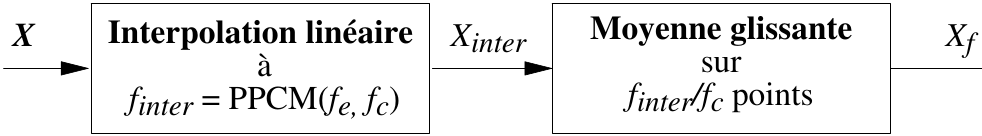
\includegraphics[width=0.8\linewidth]{images/algo_Filtre_moy.png}
\captionof{figure}{Sch�ma fonctionnel de \operfmt{Filtre\_moy}}
\label{fig:algo_Filtre_moy}
}

%%%%%COMMENTAIRE%%%%
\itemstyle{Commentaire~:}
Le passage par PPCM($f_e$, $f_c$) permet de lever l'obligation 
que $f_e$ soit un multiple de $f_c$, mais impose de 
nouvelles conditions :
\begin{itemize}
\item Si $f_c$ est inf�rieure � 1, il peut y avoir des probl�mes
d'arrondi (par ex, 1/15 = 6,666666667e-2, puis ppcm (1/15, 1)=9
au lieu de 1.
\item De fa�on g�n�rale, si PPCM($f_e$, $f_c$) est trop grand, il est
pr\'ef\'erable d'employer une autre technique.
\end{itemize}

%%%%%AUTEUR%%%%
\itemstyle{Auteur~:}
CNRM/GMEI/TRAMM

%%%%%REFERENCE%%%%
\itemstyle{R\'ef\'erences~:}

\newpage
%%%%%
%
\section{Filtre num�rique �quivalent � un circuit �lectrique RC}

\itemstyle{Op\'erateur~:} {\sf Filtre\_RC}
\index{Filtre\_RC}

%%%%%OBJET%%%%
\itemstyle{Objet~:}
Cet op�rateur applique � un param\`etre un filtrage num�rique �quivalent
� un circuit �lectrique RC. Il est d�fini par sa constante de temps $\tau$\\ 
Les caract�ristiques du filtre sont les suivantes : \\
\begin{itemize}
\item R�ponse � un cr�neau d'amplitude $X_0$ : 
$X_f = X_0 . ( 1 - e^{-\frac{t}{\tau}} )$   
\item Fonction de transfert en transform�e de Laplace :  
$ H(p) = \frac{1/\tau}{p.(p+1/\tau)} $
\item Fonction de transfert en transform\'ee en Z :
$H(Z) = \frac{1 - e^{-Te/\tau} }{ Z - e^{ -Te/\tau} } $ 
\item Fr�quence de coupure � 3dB : $f_c = \frac{1}{2\pi\tau} $ 
\end{itemize}

%%%%%ARGUMENTS%%%%
\bigskip
%%%%%ENTREES%%%%
\begin{tabarg}
\multicolumn{3}{l}{\titretab {Entr\'ees}}\\
\hline
$X$ & Vecteur, {\tt float} & Param�tre d'entr�e \\
$f_e$ & Coeff., {\tt float} & Fr�quence d'�chantillonnage de $X$ (Hz)\\
$\tau$ & Coeff., {\tt float} & Constante de temps du filtre ($s$)\\
\end{tabarg}

\medskip
%%%%%SORTIES%%%%
\begin{tabarg}
\multicolumn{3}{l}{\titretab {Sorties}}\\
\hline
$X_f$ & Vecteur, {\tt float} & Param\`etre filtr\'e (m\^eme unit\'e que $X$)\\
\end{tabarg}


%%%%%FORMULE%%%%
\itemstyle{Formule}

%%Filtre_RC_sdph
\[
X_f[i] = e^{-\frac{1}{f_e.\tau}}.X_f[i-1] +
         \left( 1 - e^{-\frac{1}{f_e.\tau}} \right). X[i-1]
\]



%%%%%AUTEUR%%%%
\itemstyle{Auteur~:}
CNRM/GMEI/TRAMM

%%%%%REFERENCE%%%%
\itemstyle{R\'ef\'erences~:}

\newpage
%%%%%
%
\section{Filtre num�rique �quivalent � un circuit RC sans d�phasage du signal de sortie}

\itemstyle{Op\'erateur~:} \operfmt{Filtre\_RC\_sdph}
\index{Filtre\_RC\_sdph}

%%%%%OBJET%%%%
\itemstyle{Objet~:}
Cet op�rateur applique � un param\`etre un filtrage num�rique �quivalent
� un circuit �lectrique RC. Il est d�fini par sa fr�quence de coupure � -3dB $f_c$.

L'utilisateur sp�cifie si l'op�rateur doit appliquer un filtre passe-bas ou 
passe-haut avec l'argument $Type$.

%%%%%ARGUMENTS%%%%
\bigskip
%%%%%ENTREES%%%%
\begin{tabarg}
\multicolumn{3}{l}{\titretab {Entr\'ees}}\\
\hline
$X$ & Vecteur, {\tt float} & Param�tre d'entr�e \\
$f_c$ & Coeff., {\tt float} & Fr�quence de coupure du filtre ($Hz$)\\
$Type$ & Coeff., {\tt Int\_32} & Type de filtre (0 : passe-bas, 1: passe-haut)\\
\end{tabarg}

\medskip
%%%%%SORTIES%%%%
\begin{tabarg}
\multicolumn{3}{l}{\titretab {Sorties}}\\
\hline
$X_f$ & Vecteur, {\tt float} & Param�tre filtr� (m�me unit� que $X$) \\
\end{tabarg}


%%%%%FORMULE%%%%
\itemstyle{Formule}

%%Filtre_RC
\[
X_f[i] = e^{-\frac{2\pi.f_c}{f_e}}.X_f[i-1] + 
         \left( 1 - e^{-\frac{2\pi.f_c}{f_e}} \right). X[i]
\]
si $Type = 1$ alors $X_f = X - X_f$


%%%%%COMMENTAIRE%%%%
\itemstyle{Commentaire~:}
Cet op�rateur prend en compte des vecteurs 1D et 2D.

%%%%%AUTEUR%%%%
\itemstyle{Auteur~:}
CNRM/GMEI/TRAMM

%%%%%REFERENCE%%%%
\itemstyle{R\'ef\'erences~:}

\newpage
%%%%%
%
%% Dans ce fichier, les �ventuels accents sont cod�s
%% en ISO-8859-15 (aka latin9)
%% La ligne suivante donne trois exemples 
%% e accent aigu : �, e accent grave : �, e-dans-l'o : �
\section{Filtre num�rique �quivalent � un circuit RC sans d�phasage du signal de sortie sur des plages temporelles}

\itemstyle{Op\'erateur~:} \operfmt{Filtre\_RC\_sdph\_paliers}
\index{Filtre\_RC\_sdph\_paliers}

%%%%%OBJET%%%%
\itemstyle{Objet~:}
Cet op�rateur applique � un param\`etre un filtrage num�rique �quivalent
� un circuit �lectrique RC. Il est d�fini par sa fr�quence de coupure � -3dB $f_c$.

L'utilisateur sp�cifie si l'op�rateur doit appliquer un filtre passe-bas ou 
passe-haut avec l'argument $Type$.

Le filtrage est effectu� sur les plages temporelles d�finies en entr�e. En dehors de ces plages temporelles on trouvera des valeurs manquantes.


%%%%%ARGUMENTS%%%%
\bigskip
%% Dans ce fichier, les �ventuels accents sont cod�s
%% en ISO-8859-15 (aka latin9)
%% La ligne suivante donne trois exemples 
%% e accent aigu : �, e accent grave : �, e-dans-l'o : �
%%%%%ENTREES%%%%
\begin{tabarg}
\multicolumn{3}{l}{\titretab {Entr\'ees}}\\
\hline
$X$ & Vecteur, {\tt float} & Param�tre d'entr�e \\
$f_c$ & Coeff., {\tt float} & Fr�quence de coupure du filtre ($Hz$)\\
$Type$ & Coeff., {\tt Int\_32} & Type de filtre (0 : passe-bas, 1: passe-haut)\\
$time_out$ & Vecteur, {\tt float} & R�f�rence de temps qui d�finit les plages de calcul \\
\end{tabarg}

\medskip
%%%%%SORTIES%%%%
\begin{tabarg}
\multicolumn{3}{l}{\titretab {Sorties}}\\
\hline
$X_out$ & Vecteur, {\tt float} & Param\`etre filtr\'e (m\^eme unit\'e que $X$) \\
\end{tabarg}


%%%%%FORMULE%%%%
\itemstyle{Formule}

%% Formule de l'operateur : Filtre_RC_sdph_paliers
%% Dans ce fichier, les �ventuels accents sont cod�s
%% en ISO-8859-15 (aka latin9)
%% La ligne suivante donne trois exemples 
%% e accent aigu : �, e accent grave : �, e-dans-l'o : �
\[
X_f[i] = e^{-\frac{2\pi.f_c}{f_e}}.X_f[i-1] + 
         \left( 1 - e^{-\frac{2\pi.f_c}{f_e}} \right). X[i]
\]
si $Type = 1$ alors $X_f = X - X_f$



%%%%%AUTEUR%%%%
\itemstyle{Auteur~:}
CNRM/GMEI/TRAMM

%%%%%REFERENCE%%%%
\itemstyle{R\'ef\'erences~:}

\newpage
%%%%%
%
\section{Lissage de donn�es}

\itemstyle{Op\'erateur~:} {\sf Oliver\_lisse}
\index{Oliver\_lisse}

%%%%%OBJET%%%%
\itemstyle{Objet~:}
On remplace chaque valeur par une moyenne pond�r�e des n derni�res valeurs en
affectant � chaque valeur un poids inversement proportionnel � son �loignement.

%%%%%ARGUMENTS%%%%
\bigskip
%%%%%ENTREES%%%%
\begin{tabarg}
\multicolumn{3}{l}{\titretab {Entr\'ees}}\\
\hline
$Ve$ & Vecteur, {\tt float} & Vecteur de donn�es quelconques\\
$Pas$ & Coeff., {\tt float} & Nombre de valeurs entrant dans la moyenne\\
\end{tabarg}

\medskip
%%%%%SORTIES%%%%
\begin{tabarg}
\multicolumn{3}{l}{\titretab {Sorties}}\\
\hline
$Vs$ & Vecteur, {\tt float} & Vecteur contenant les donn�es liss�es (m�me unit� que $Ve$)\\
\end{tabarg}


%%%%%FORMULE%%%%
\itemstyle{Formule}

%%Oliver_lisse
\[
Vs[i] = \frac{\sum_{n= 0}^{Pas} (Pas-n) . Ve[i-n]} {\sum_{n= 0}^{Pas} (Pas-n)}
\]


%%%%%AUTEUR%%%%
\itemstyle{Auteur~:}
CNRM/GMEI/TRAMM

%%%%%REFERENCE%%%%
\itemstyle{R\'ef\'erences~:}
Olivier Traull� / GMEI / 4M

\newpage
%%%%%
%
\section{�chantillonnage et skewness d'une variable sur une nouvelle base
de temps donn�e par un time\_{bnds}}

\itemstyle{Op\'erateur~:} \textsf{Skewness\_tps\_{bnds}}
\index{Skewness\_tps\_bnds}

%%%%%OBJET%%%%
\itemstyle{Objet~:}
Cette fonction calcule, pour chaque instant $t$ d'une
base de temps $time_{out}$, 
une variable $X_{out}$, contenant le skewness des
valeurs de  $X_{in}$ entre les bornes donn�es par le $time_{bnds}$ associ� � $time_{out}$.

Aucune supposition n'est faite sur la r�gularit� de
l'�chantillonnage des 2 variables. Cette fonction peut
donc servir, par exemple, � transformer une s�rie temporelle
asynchrone en une s�rie r�guli�re. Il est cependant n�cessaire
que $time_{in}$ (le temps de $X_{in}$) soit "� peu pr�s" tri� par ordre
croissant.


%%%%%ARGUMENTS%%%%
\bigskip
%%%%%ENTREES%%%%
\begin{tabarg}
\multicolumn{3}{l}{\titretab {Entr\'ees}}\\
\hline
$X_{in}$ & Vecteur, \texttt{float} & Variable d'origine\\
$toler_{mnq}$ & Coeff., \texttt{float} & Seuil de calcul de la moyenne (pourcentage). A chaque instant de la base de temps d'arriv�e, 
le skewness est calcul�e si le pourcentage d'�chantillons dans l'intervalle de temps est strictement sup�rieur � $toler_{mnq}$. Sinon,le r�sultat est "valeur manquante". Si $toler_{mnq}$ = 100, le calcul est fait d�s qu'il y a au moins une valeur valide dans l'�chantillon. \\
$time_{out}$ & Vecteur, \texttt{double} & Base de temps d'arriv�e (secondes)\\
\end{tabarg}

\medskip
%%%%%SORTIES%%%%
\begin{tabarg}
\multicolumn{3}{l}{\titretab {Sorties}}\\
\hline
$X_{out}$ & Vecteur, \texttt{float} & skewness de $X_{in}$ �chantillonn� sur
la base de $time_{out}$ (m�me unit� que $X_{in})$\\
\end{tabarg}



%%%%%FORMULE%%%%
\itemstyle{Formule}

%% Skewness_tps_bnds
Pour  i=$0$, Nbre $Time_{bnds}$ :

\[
X_{out}[i] = skew(\displaystyle{X_{in\_tb}})
\]

$X_{in\_tb}$ sont les valeurs de $X_{in}$ entre les temps $Time_{bnds}[i][0]$ et $Time_{bnds}[i][1]$.



%%%%COMMENTAIRE%%%%
\itemstyle{Commentaire~:}
\textit{$Time_{bnds}$} est un tableau d'intervalles de temps d�termin�s � partir du vecteur temps $time_{out}$.

%%%%%AUTEUR%%%%
\itemstyle{Auteur~:}
CNRM/GMEI/TRAMM

%%%%%REFERENCE%%%%
\itemstyle{R\'ef\'erences~:}
N�ant.


\chapter{Thermodynamique}

%% THERMODYNAMIQUE %%
%
\section{Pressions et angles d'incidence }

\itemstyle{ Op\'erateur~: } {\sf Pression}
\index{Pression}

%%%%%OBJET%%%%%
\itemstyle{ Objet~: }
Calcul de la pression statique et de la 
surpression dynamique par correction  de l'erreur de 
statique, et 
calcul des angles d'incidence et de d\'erapage \`a 
partir des pressions diff\'erentielles mesur\'ees suivant
la verticale et l'horizontale de l'avion. \newline

%%%%%ARGUMENTS%%%%%
\bigskip
%%%%%ENTREES%%%%
\begin{tabarg}
\multicolumn{3}{l}{\titretab{Entr\'ees}}\\
\hline
$P_{sb}$ & Vecteur, {\tt float} & Pression statique brute ($hPa$)\\
$\Delta P_b$ & Vecteur, {\tt float} & Pression dynamique brute ($hPa$) \\
$\Delta P_h$ & Vecteur, {\tt float} & Pression diff\'erentielle mesur\'ee suivant l'horizontale de l'avion ($hPa$) \\
$\Delta P_v$ & Vecteur, {\tt float} & Pression diff\'erentielle mesur\'ee suivant la verticale de l'avion ($hPa$) \\
$C_{\alpha}$ & Coeff., {\tt float[2]} & Coefficients de calibration d'incidence \\
$C_{\beta} $  & Coeff., {\tt float[2]} & Coefficients de calibration de d\'erapage\\
$C_{errstat} $  & Coeff., {\tt float[4]} & Coefficients de calcul de l'erreur de statique \\
\end{tabarg}

\medskip
%%%%%SORTIES%%%%
\begin{tabarg}
\multicolumn{3}{l}{\titretab{Sorties}}\\
\hline
$P_s$ & Vecteur, {\tt float} & Pression statique ($hPa$)\\
$\alpha$ & Vecteur, {\tt float} & Angle d'incidence ($rad$)\\
$\beta$ & Vecteur, {\tt float} & Angle de d\'erapage ($rad$)\\
$\Delta P$ & Vecteur, {\tt float} & Pression dynamique corrig\'ee de l'erreur de statique ($hPa$)
\end{tabarg}


%%%%%FORMULE%%%%
\itemstyle{ Formule }

%%%% THERMODYNAMIQUE
Si $\Delta P_b > 25 $hPa,
\[
Errstat = C_{errstat}[0] + C_{errstat}[1].\Delta P_b +
	  C_{errstat}[2].\Delta P_b^2 + C_{errstat}[3].\Delta P_b^3 
\]
sinon
\[
Errstat =  {{\Delta P_b} \over 25} . Errstat(25)
\]
\[
P_s = P_{sb} - Errstat
\]
$$
\Delta P = \Delta P_b + Errstat
$$
$$
\alpha = C_{\alpha}[0] + C_{\alpha}[1]. \frac{ \Delta P_v}{\Delta P}
$$
$$
\beta = C_{\beta}[0] + C_{\beta}[1]. \frac{ \Delta P_h}{\Delta P}
$$


%%%%COMMENTAIRE%%%%
\itemstyle{ Commentaire~:}

L'erreur de statique est calcul\'ee \`a partir de
la pression dynamique brute, par un polyn\^ome du 3$^{eme}$
degr\'e dans la gamme [25,90] hPa (la gamme de vol normal), et
par une interpolation dans la gamme [0,25] hPa.


%%%%%AUTEUR%%%%%
\itemstyle{ Auteur~:}
CNRM/GMEI/TRAMM

%%%%%REFERENCES%%%%%
\itemstyle{ R\'ef\'erences~:}

\newpage
%%%%%
%
\section{Erreur �de statique� en fonction de la pression dynamique et
des angles d'attitude}

\itemstyle{Op\'erateur~:} {\sf Errstat\_Allet99}
\index{Errstat\_Allet99}

%%%%%OBJET%%%%
\itemstyle{Objet~:}

Cet op\'erateur calcule l'erreur sur la mesure de pression 
statique de l'avion comme une combinaison lin�aire de la surpression dynamique, 
de la pression statique brute, des angles de tangage et de
roulis de l'avion. 

%%%%%ARGUMENTS%%%%
\bigskip
%%%%%ENTREES%%%%
\begin{tabarg}
\multicolumn{3}{l}{\titretab {Entr\'ees}}\\
\hline
$P_s$ & Vecteur, {\tt float} & Pression statique brute ($hPa$)\\
$\theta$ & Vecteur, {\tt float} & Angle de tangage de l'avion ($degres$)\\
$\phi$ & Vecteur, {\tt float} & Angle de roulis de l'avion ($degres$)\\
$\Delta P$ & Vecteur, {\tt float} & Surpression dynamique ($hPa$)\\
$C_0$ & Coeff., {\tt float} & Coefficient de calibration\\
$C_1$ & Coeff., {\tt float} & Coefficient de calibration\\
$C_2$ & Coeff., {\tt float} & Coefficient de calibration\\
$C_3$ & Coeff., {\tt float} & Coefficient de calibration\\
$C_4$ & Coeff., {\tt float} & Coefficient de calibration\\
\end{tabarg}

\medskip
%%%%%SORTIES%%%%
\begin{tabarg}
\multicolumn{3}{l}{\titretab {Sorties}}\\
\hline
$Errstat$ & Vecteur, {\tt float} &  Erreur de pression statique ($hPa$)\\
\end{tabarg}


%%%%%FORMULE%%%%
\itemstyle{Formule}

%%Errstat_Allet99
$$
Errstat = C_0 + C_1.P_s+ 
                C_2.\theta +
                C_3.\phi +
                C_4.\Delta P \\ 
$$


%%%%%AUTEUR%%%%
\itemstyle{Auteur~:}
CNRM/GMEI/TRAMM

%%%%%REFERENCE%%%%
\itemstyle{R\'ef\'erences~:}
Cette correction a �t� mise au point par Ch. Allet (INSU/Voloth�que)
pour la calibration de l'avion ARAT (Janvier 99). 

\newpage
%% THERMODYNAMIQUE %%
%
\section{Altitude pression}

\itemstyle{ Op\'erateur~: } {\sf AltiPress}
\index{AltiPress}

%%%%%OBJET%%%%%
\itemstyle{ Objet~: }
Calcul de l'altitude pression, \`a 
partir de la temp\'erature virtuelle.

%%%%%ARGUMENTS%%%%
\bigskip
%%%%%ENTREES%%%%
\begin{tabarg}
\multicolumn{3}{l}{\titretab{Entr\'ees}}\\
\hline
$T_v$ & Vecteur, \texttt{float} & Temp\'erature virtuelle ($K$ ou $^\circ C$)\\
$P_s$ & Vecteur, \texttt{float} & Pression statique ($hPa$) \\
$QNH$ & Coeff.,  \texttt{float} & Pression au sol ($hPa$) \\
$R_a/g$ & Coeff., \texttt{float} & Rapport de la constante sp\'ecifique de
l'air sec sur l'acc\'el\'eration de la pesanteur\\
\end{tabarg}

\medskip
%%%%%SORTIES%%%%
\begin{tabarg}
\multicolumn{3}{l}{\titretab{Sorties}}\\
\hline
$Alti\_p$ & Vecteur, \texttt{float} & Altitude pression ($m$)\\
\end{tabarg}



%%%%%FORMULE%%%%
\itemstyle{ Formule }

%%% Altitude pression 
\[
Alti\_p = \frac{R_a}{g}.T_v.\log \left( \frac{QNH}{Ps} \right)
\]


Avec $T_v$ exprim\'e en K.

%%%%%AUTEUR%%%%%
\itemstyle{ Auteur~:}
CNRM/GMEI/TRAMM

%%%%%REFERENCES%%%%%
\itemstyle{ R\'ef\'erences~:}
Triplet-Roche \cite{Triplet-Roche}.

\newpage
%%%%%
%
%% Dans ce fichier, les �ventuels accents sont cod�s
%% en ISO-8859-15 (aka latin9)
%% La ligne suivante donne trois exemples 
%% e accent aigu : �, e accent grave : �, e-dans-l'o : �
\section{Estimation de la pression � une altitude donn�e}

\itemstyle{Op\'erateur~:} \operfmt{PressAlti}
\index{PressAlti}

%%%%%OBJET%%%%
\itemstyle{Objet~:}
Calcul de la pression � une altitude donn�e � partir d'une mesure 
de pression � une autre altitude.

%%%%%ARGUMENTS%%%%
\bigskip
%% Dans ce fichier, les �ventuels accents sont cod�s
%% en ISO-8859-15 (aka latin9)
%% La ligne suivante donne trois exemples 
%% e accent aigu : �, e accent grave : �, e-dans-l'o : �
%%%%%ENTREES%%%%
\begin{tabarg}
\multicolumn{3}{l}{\titretab {Entr\'ees}}\\
\hline
$P_0$ & Vecteur, \texttt{float} &  Pression au niveau $Z_0$ (hPa)\\
$T_m$ & Vecteur, \texttt{float} & Temp�rature moyenne de la couche (Kelvin ou Celsius )\\
$Z_0$ & Coeff., \texttt{float} & Altitude de la pression $P_0$ (m)\\
$Z$ & Coeff., \texttt{float} & Altitude  (m)\\
$R_a/g$ & Coeff., \texttt{float} & Rapport de la constante sp\'ecifique de
l'air sec sur l'acc\'el\'eration de la pesanteur\\
\end{tabarg}

\medskip
%%%%%SORTIES%%%%
\begin{tabarg}
\multicolumn{3}{l}{\titretab {Sorties}}\\
\hline
$P$ & Vecteur, \texttt{float} & Pression estim�e \`a l'altitude Z (hPa)\\
\end{tabarg}


%%%%%FORMULE%%%%
\itemstyle{Formule}

%% Formule de l'operateur : PressAlti
%% Dans ce fichier, les �ventuels accents sont cod�s
%% en ISO-8859-15 (aka latin9)
%% La ligne suivante donne trois exemples 
%% e accent aigu : �, e accent grave : �, e-dans-l'o : �
\[
P_s = P_0 . exp \left( \frac{ Z_0 - Z }{\frac{R_a}{g}. T_m } \right)   
\]



%%%%%AUTEUR%%%%
\itemstyle{Auteur~:}
CNRM/GMEI/TRAMM

%%%%%REFERENCE%%%%
\itemstyle{R\'ef\'erences~:}
Triplet-Roche \cite{Triplet-Roche}.

\newpage
%%%%%
%
%% Dans ce fichier, les �ventuels accents sont cod�s
%% en ISO-8859-15 (aka latin9)
%% La ligne suivante donne trois exemples 
%% e accent aigu : �, e accent grave : �, e-dans-l'o : �
\section{Calcul de la pression OACI � partir de l'altitude}

\itemstyle{Op\'erateur~:} \operfmt{PressAltiOACI}
\index{PressAltiOACI}

%%%%%OBJET%%%%
\itemstyle{Objet~:}
Calcul de la pression � partir de l'altitude selon la norme OACI 1993

%%%%%ARGUMENTS%%%%
\bigskip
%% Dans ce fichier, les �ventuels accents sont cod�s
%% en ISO-8859-15 (aka latin9)
%% La ligne suivante donne trois exemples 
%% e accent aigu : �, e accent grave : �, e-dans-l'o : �
%%%%%ENTREES%%%%
\begin{tabarg}
\multicolumn{3}{l}{\titretab {Entr\'ees}}\\
\hline
$h$ & Vecteur, \texttt{float} & altitude geographique(m)\\
\end{tabarg}

\medskip
%%%%%SORTIES%%%%
\begin{tabarg}
\multicolumn{3}{l}{\titretab {Sorties}}\\
\hline
$P$ & Vecteur, \texttt{float} & pression (hPa)\\
\end{tabarg}


%%%%%FORMULE%%%%
\itemstyle{Formule}

%% Formule de l'operateur : PressAltiOACI
%% Dans ce fichier, les �ventuels accents sont cod�s
%% en ISO-8859-15 (aka latin9)
%% La ligne suivante donne trois exemples 
%% e accent aigu : �, e accent grave : �, e-dans-l'o : �


Altitude g�opotentielle $H= (\frac{r*h}{r+h}) $\\
Rayon de la terre r=6356766,0 m\\
Acc�leration normalis�e de la pesanteur  $g_0$ = 9,80665 $m/s^2$ \\
Constante massique des gaz parfaits sp�cifique de l'air  R  = 287,05287 $J/(K*kg)$\\

Si H inf�rieure � -5000 m  \\
 hors de la norme OACI, $P=misval$\\

Si H comprise entre -5000 et 0 m  \\
$P = P_b[1+ \frac{\beta }{T_b}(H-H_b)]^{(\frac{-g_0}{\beta R})}$\\
avec $P_b$ = 1776,87 hPa\\
et $\beta$ = -0,0065 K/m\\
et  $T_b$ = 320,65 K\\
et  $H_b$  = -5000,0 m\\

Si H comprise entre 0 et 11000 m  \\
$P = P_b[1+ \frac{\beta }{T_b}(H-H_b)]^{(\frac{-g_0}{\beta R})}$ \\
avec $P_b$ = 1013,25 hPa\\
et $\beta$ = -0,0065 K/m\\
et  $T_b$ = 288,15 K\\
et  $H_b$  = 0,0 m\\

Si H comprise entre 11000 et 20000 m \\
$P = P_b e^{\frac{-g_0}{R T}(H-H_b)}$ \\
avec $P_b$ = 226,320 hPa\\
et $\beta$ = 0 K/m\\
et  $T$ = 216,65 K\\
et  $H_b$  = 11000,0 m\\

Sinon si H sup�rieure �  20000 m  \\
 $P=misval$\\



%%%%%AUTEUR%%%%
\itemstyle{Auteur~:}
CNRM/GMEI/TRAMM

%%%%%REFERENCE%%%%
\itemstyle{R\'ef\'erences~:}
MANUEL DE L'ATMOSPHERE TYPE OACI \cite{OACI-93}

\newpage
%%%%%
%
%% Dans ce fichier, les �ventuels accents sont cod�s
%% en ISO-8859-15 (aka latin9)
%% La ligne suivante donne trois exemples 
%% e accent aigu : �, e accent grave : �, e-dans-l'o : �
\section{Estimation de la pression � des altitudes donn�es}

\itemstyle{Op\'erateur~:} \operfmt{PressAltiVect}
\index{PressAltiVect}

%%%%%OBJET%%%%
\itemstyle{Objet~:}
Calcul de la pression � des altitudes donn�es � partir d'une mesure 
de pression � d'autres altitudes.

%%%%%ARGUMENTS%%%%
\bigskip
%% Dans ce fichier, les �ventuels accents sont cod�s
%% en ISO-8859-15 (aka latin9)
%% La ligne suivante donne trois exemples 
%% e accent aigu : �, e accent grave : �, e-dans-l'o : �
%%%%%ENTREES%%%%
\begin{tabarg}
\multicolumn{3}{l}{\titretab {Entr\'ees}}\\
\hline
$P_0$ & Vecteur, \texttt{float} &  Pression au niveau $Z_0$ (hPa)\\
$T_m$ & Vecteur, \texttt{float} & Temp�rature moyenne de la couche (Kelvin ou Celsius )\\
$Z_0$ & Vecteur, \texttt{float} & Altitude de la pression $P_0$ (m)\\
$Z$ & Vecteur, \texttt{float} & Altitude  (m) pour laquelle on calcule la pression\\
$R_a/g$ & Coeff., \texttt{float} & Rapport de la constante sp\'ecifique de
l'air sec sur l'acc\'el\'eration de la pesanteur\\
\end{tabarg}

\medskip
%%%%%SORTIES%%%%
\begin{tabarg}
\multicolumn{3}{l}{\titretab {Sorties}}\\
\hline
$P$ & Vecteur, \texttt{float} & Pression estim�e \`a l'altitude Z (hPa)\\
\end{tabarg}


%%%%%FORMULE%%%%
\itemstyle{Formule}

%% Formule de l'operateur : PressAlti
%% Dans ce fichier, les �ventuels accents sont cod�s
%% en ISO-8859-15 (aka latin9)
%% La ligne suivante donne trois exemples 
%% e accent aigu : �, e accent grave : �, e-dans-l'o : �
\[
P_s = P_0 . exp \left( \frac{ Z_0 - Z }{\frac{R_a}{g}. T_m } \right)   
\]



%%%%%AUTEUR%%%%
\itemstyle{Auteur~:}
CNRM/GMEI/TRAMM

%%%%%REFERENCE%%%%
\itemstyle{R\'ef\'erences~:}
Triplet-Roche \cite{Triplet-Roche}.

\newpage
%%%%%
%
%% Dans ce fichier, les �ventuels accents sont cod�s
%% en ISO-8859-15 (aka latin9)
%% La ligne suivante donne trois exemples 
%% e accent aigu : �, e accent grave : �, e-dans-l'o : �
\section{Calcul de l'altitude en fonction de la pression selon la norme OACI}

\itemstyle{Op\'erateur~:} \operfmt{AltiPressOACI}
\index{AltiPressOACI}

%%%%%OBJET%%%%
\itemstyle{Objet~:}
Calcul de l'altitude en fonction de la pression selon la norme OACI

%%%%%ARGUMENTS%%%%
\bigskip
%% Dans ce fichier, les �ventuels accents sont cod�s
%% en ISO-8859-15 (aka latin9)
%% La ligne suivante donne trois exemples 
%% e accent aigu : �, e accent grave : �, e-dans-l'o : �
%%%%%ENTREES%%%%
\begin{tabarg}
\multicolumn{3}{l}{\titretab {Entr\'ees}}\\
\hline
$P$ & Vecteur, \texttt{float} & pression (hPa)\\
\end{tabarg}

\medskip
%%%%%SORTIES%%%%
\begin{tabarg}
\multicolumn{3}{l}{\titretab {Sorties}}\\
\hline
$H$ & Vecteur, \texttt{float} & altitude g�opotentielle (m)\\
$h$ & Vecteur, \texttt{float} & altitude g�ographique (m)\\
\end{tabarg}


%%%%%FORMULE%%%%
\itemstyle{Formule}

%% Formule de l'operateur : AltiPressOACI
%% Dans ce fichier, les �ventuels accents sont cod�s
%% en ISO-8859-15 (aka latin9)
%% La ligne suivante donne trois exemples 
%% e accent aigu : �, e accent grave : �, e-dans-l'o : �

$P_{-5000}=1776,87$ hPa(pression pour une altitude geopotentielle de -5000m)\\
$P_0=1013,25 $ hPa(pression pour une altitude geopotentielle de 0m) \\
$P_{11000}=226,320 $ hPa(pression pour une altitude geopotentielle de 11000m)\\
$P_{20000}=54,7487 $ hPa(pression pour une altitude geopotentielle de 20000m)\\

Rayon de la terre r=6356766.0 m\\
Acceleration normalisee de la pesanteur  $g_0 = 9,80665 m/{s^2}$ \\
Constante massique des gaz parfaits sp�cifique de l'air  $R  = 287,05287 J/(K*kg)$\\

Si P superieure � $P_{-5000}$  \\
 hors de la norme OACI, $P=misval$\\

Si P comprise entre $P_{-5000}$ et $P_0$  \\
$H =\left[\left(\frac{P}{P_b}\right)^ {\frac{-\beta *R}{g_0}}-1.0\right]*(T_b/\beta )+H_b$\\
avec $P_b$ = $P_{-5000}$\\
et $\beta$ = -0,0065 K/m\\
et  $T_b$ = 320,65 K\\
et  $H_b$  = -5000,0 m\\

Si P comprise entre $P_0$ et $P_{11000} $\\
$H =\left[\left(\frac{P}{P_b}\right)^ {\frac{-\beta *R}{g_0}}-1.0\right]*(T_b/\beta )+H_b$\\
avec $P_b$ = $P_0$\\
et $\beta$ = -0,0065 K/m\\
et  $T_b$ = 288,15 K\\
et  $H_b$  = 0,0 m\\

Si P comprise entre $P_{11000}$ et $P_{20000}$\\
$H = log(P/P_b)*\frac{R*T}{-g_0}+H_b$ \\
avec $P_b$ = $P_{11000}$\\
et  $T$ = 216,65 K\\
et  $H_b$  = 11000,0 m\\

Si P inferieure �  $P_{20000}$  \\
  $P=misval$\\

Valeur de h \\
$h=\frac{(r*H)}{(r-H)}$


%%%%%AUTEUR%%%%
\itemstyle{Auteur~:}
CNRM/GMEI/TRAMM

%%%%%REFERENCE%%%%
\itemstyle{R\'ef\'erences~:}
MANUEL DE L'ATMOSPHERE TYPE OACI\cite{OACI-93}

\newpage
%%%%%
%
\section{Calcul incr�mental d'altitude pression}

\itemstyle{Op\'erateur~:} \operfmt{AltiPressInc}
\index{AltiPressInc}

%%%%%OBJET%%%%
\itemstyle{Objet~:}
Calcul d'une altitude-pression de mani�re incr�mentale 
le long de la trajectoire par la formule de Laplace
(Z$_2$ = Z$_{1}$ + $Ra/g <Tv> log (P_{1}/P_2)$.

%%%%%ARGUMENTS%%%%
\bigskip
%%%%%ENTREES%%%%
\begin{tabarg}
\multicolumn{3}{l}{\titretab {Entr\'ees}}\\
\hline
$Tv$ & Vecteur, \texttt{float} & Temp�rature virtuelle (�C ou Kelvin)\\
$Ps$ & Vecteur, \texttt{float} & Pression statique (hPa)\\
ref\_time & Vecteur, \texttt{double} & Datation des mesures (sec)\\
$S0$ & Coeff., \texttt{double} & Instant de r�f�rence (sec)\\
$Z0$ & Coeff., \texttt{float} & Altitude � l'instant $S0$ (m)\\
$R_a/g$ & Coeff., \texttt{float} & Rapport de la constante sp\'ecifique de
l'air sec sur l'acc\'el�ration de la pesanteur\\
\end{tabarg}

\medskip
%%%%%SORTIES%%%%
\begin{tabarg}
\multicolumn{3}{l}{\titretab {Sorties}}\\
\hline
$Z$ & Vecteur, \texttt{float} & Altitude pression (m)\\
\end{tabarg}


%%%%%FORMULE%%%%
\itemstyle{Formule}

%%% Altitude pression incr�mentale
$Tv$ est convertie en Kelvin, si besoin est, puis :
\begin{align*}
Z_{i0} &= Z0 \qquad \text{ avec } i0 \text{ tq.  ref\_time}_{i0} = S0\\
Z_j &= Z_{i} + \frac{R_a}{g}.\left(\frac{Tv_j+Tv_{i}}{2}\right).\log \left( \frac{Ps_{i}}{Ps_j} \right) \qquad \text{avec} 
\begin{cases}
i = j+1 \text{ pour } j<i0\\
i = j-1 \text{ pour } j>i0
\end{cases}
\end{align*}



%%%%%AUTEUR%%%%
\itemstyle{Auteur~:}
CNRM/GMEI/TRAMM

%%%%%REFERENCE%%%%
\itemstyle{R\'ef\'erences~:}
Triplet-Roche \cite{Triplet-Roche} (p.92 de l'�dition de 1977).
%Fondamentaux de M�t�orologie, \cite{Malardel} (p.299 de la seconde �dition).


\newpage
%% THERMODYNAMIQUE %%

\section{Correction de la pression dynamique rad\^ome}

\itemstyle{ Op\'erateur~: } {\sf Cor\_dPrad\_angle} 
\index{Cor\_dPrad\_angle}

%%%%%OBJET%%%%%
\itemstyle{ Objet~: }
Correction de l'erreur sur la mesure de pression dynamique
r\'ealis\'ee avec le trou central du rad\^ome due \`a l'angle
du vent relatif.

%%%%%ARGUMENTS%%%%%
\bigskip
%%%%%ENTREES%%%%
\begin{tabarg}
\multicolumn{3}{l}{\titretab{ Entr\'ees}}\\
\hline
$\Delta P_b$ & Vecteur, {\tt float} & Pression dynamique mesur\'ee ($hPa$)\\
$\alpha$ & Vecteur, {\tt float} & Angle d'incidence ($rad$)\\
$\beta$ & Vecteur, {\tt float} & Angle de d\'erapage ($rad$) \\
\end{tabarg}

\medskip
%%%%%SORTIES%%%%
\begin{tabarg}
\multicolumn{3}{l}{\titretab{ Sorties}}\\
\hline
$\Delta P_c$ & Vecteur, {\tt float} & Pression dynamique corrig\'ee (m\^eme unit\'e que $\Delta
P_b$)\\
\end{tabarg}


%%%%%FORMULE%%%%
\itemstyle{ Formule }


% formules de correction de la pression dyn.
% radome en fct. des angles d'incidences et 
% de derapage

$$
\Delta P_c = \frac{4 . \Delta P_b}
                  { 9.\cos \alpha .\cos \beta - 5 }
$$


%%%%%AUTEUR%%%%%
\itemstyle{ Auteur~:}
CNRM/GMEI/TRAMM

%%%%%REFERENCES%%%%%
\itemstyle{ R\'ef\'erences~:}
Note NCAR-385 de P. Nacass \cite{Nacass-92}.

\newpage
%% THERMODYNAMIQUE %%
%
\section{Temp\'erature statique}

\itemstyle{Op\'erateur~:} \operfmt{Tair}
\index{Tair}

%%%%%OBJET%%%%
\itemstyle{Objet~:}
Calcul de la temp\'erature statique de l'air, \`a 
partir de la mesure de temp\'erature totale.\newline
Cet op\'erateur s'applique aux capteurs de temp\'erature par contact
de type Rosemount par exemple.

%%%%%ARGUMENTS%%%%%
\bigskip
%%%%%ENTREES%%%%
\begin{tabarg}
\multicolumn{3}{l}{\titretab{Entr\'ees}}\\
\hline
$T_t$ & Vecteur, \texttt{float} & Temp\'erature totale mesur\'ee ($K$ ou $^\circ C$)\\
$\Delta P$ & Vecteur, \texttt{float} & Pression dynamique ($hPa$) \\
$P_s$ & Vecteur, \texttt{float} & Pression statique ($hPa$) \\
$r_f$ & Coeff., \texttt{float} & Coefficient de r\'ecup\'eration de la sonde\\
$R_a/c_{pa}$ & Coeff., \texttt{float} & Rapport de la Constante sp\'ecifique de
l'air sec sur la Chaleur massique \`a pression constante de l'air sec \\
\end{tabarg}
\medskip

%%%%%SORTIES%%%%
\begin{tabarg}
\multicolumn{3}{l}{\titretab{Sorties}}\\
\hline
$T_s$ & Vecteur, \texttt{float} & Temp\'erature statique de l'air (m\^eme unit\'e que $T_t$)\\
\end{tabarg}


%%%%%FORMULE%%%%
\itemstyle{ Formule}

% Calcul de la temperature statique a 
% partir de la temperature d'impact et
% de la pression dynamique. 
\[
T_s = \frac{T_t}
     {1 + r_f\times \left( \left(1 + \frac{\Delta P}{P_s}\right)
        ^{R_a/c_{pa}} - 1\right)}
\]


Avec $T_s$ et $T_t$ exprim\'es en K.

%%%%%AUTEUR%%%%%
\itemstyle{ Auteur~:}
CNRM/GMEI/TRAMM

%%%%%REFERENCES%%%%%
\itemstyle{ R\'ef\'erences~:}

\newpage
%% THERMODYNAMIQUE %%
%
%% Dans ce fichier, les �ventuels accents sont cod�s
%% en ISO-8859-15 (aka latin9)
%% La ligne suivante donne trois exemples 
%% e accent aigu : �, e accent grave : �, e-dans-l'o : �
\section{Temp�rature statique (lorsque ventilation suffisante)}

\itemstyle{Op\'erateur~:} \operfmt{Tair\_avion}
\index{Tair\_avion}

%%%%%OBJET%%%%
\itemstyle{Objet~:}
Calcul de la temp�rature statique de l'air, � 
partir de la mesure de temp�rature totale et de la surpression dynamique.\newline
Ce calcul s'applique aux capteurs de temp�rature par contact
de type Rosemount par exemple.\newline
Le calcul n'est fait que lorsque la surpression dynamique est
sup�rieure � 6 hPa. Dans le cas contraire, signe d'une
ventilation insuffisante du capteur, la valeur retourn�e est
le code "valeur manquante".


%%%%%ARGUMENTS%%%%
\bigskip
%% Dans ce fichier, les �ventuels accents sont cod�s
%% en ISO-8859-15 (aka latin9)
%% La ligne suivante donne trois exemples 
%% e accent aigu : �, e accent grave : �, e-dans-l'o : �
%%%%%ENTREES%%%%
\begin{tabarg}
\multicolumn{3}{l}{\titretab {Entr\'ees}}\\
\hline
$T_t$ & Vecteur, \texttt{float} &  Temp�rature totale ($K$ ou $^\circ C$)\\
$\Delta P$ & Vecteur, \texttt{float} & Pression dynamique ($hPa$)\\
$P_s$ & Vecteur, \texttt{float} & Pression statique ($hPa$)\\
$r_f$ & Coeff., \texttt{float} & Coefficient de r�cup�ration du capteur utilis�\\
$R_a/c_{pa}$ & Coeff., \texttt{float} & Rapport de la constante sp�cifique de
l'air sec sur la chaleur massique � pression constante de l'air sec\\
\end{tabarg}

\medskip
%%%%%SORTIES%%%%
\begin{tabarg}
\multicolumn{3}{l}{\titretab {Sorties}}\\
\hline
$T_s$ & Vecteur, \texttt{float} & Temp�rature statique de l'air (m�me unit� que $T_t$)\\
\end{tabarg}


%%%%%FORMULE%%%%
\itemstyle{Formule}

%% Formule de l'operateur : Tair_avion
%% Dans ce fichier, les �ventuels accents sont cod�s
%% en ISO-8859-15 (aka latin9)
%% La ligne suivante donne trois exemples 
%% e accent aigu : �, e accent grave : �, e-dans-l'o : �
Si besoin est, $T_t$ est converti en Kelvin, puis
\[
T_s =
\begin{cases}
\frac{T_t}
     {1 + r_f \left( \left(1 + \frac{\Delta P}{P_s}\right)
        ^{R_a/c_{pa}} - 1\right)} \qquad \text{ si } \Delta P > 6 \\
\text{valeur\_manquante} \qquad \text{ sinon } \\
\end{cases}
\]


%%%%%AUTEUR%%%%
\itemstyle{Auteur~:}
CNRM/GMEI/TRAMM

%%%%%REFERENCE%%%%
\itemstyle{R\'ef\'erences~:}

\newpage
%% THERMODYNAMIQUE %%
%
\section{Vitesse propre}

\itemstyle{ Op\'erateur~: } {\sf V\_Air\_Ts}
\index{V\_Air\_Ts}

%%%%%OBJET%%%%%
\itemstyle{ Objet~: }
Calcul de la vitesse propre de l'air, \`a 
partir des mesures de surpression dynamique, pression 
statique, et temp\'erature statique, en employant 
une des formes de la formule de Barr\'e-St-Venant.

%%%%%ARGUMENTS%%%%%
\bigskip
%%%%%ENTREES%%%%
\begin{tabarg}
\multicolumn{3}{l}{\titretab{Entr\'ees}}\\
\hline
$T_s$ & Vecteur, {\tt float} & Temp\'erature statique ($K$ ou $^\circ C$)\\
$P_s$ & Vecteur, {\tt float} & Pression statique ($hPa$) \\
$\Delta P$ & Vecteur, {\tt float} & Pression dynamique  ($hPa$)\\
$c_{pa}$ & Coeff., {\tt float} & Chaleur massique \`a pression constante
du gaz dans lequel la mesure est faites (en g�n�ral l'air sec, 
1004 J.K$^{-1}$.kg$^{-1}$).\\
$R_a/c_{pa}$ & Coeff., {\tt float} & Rapport de la Constante sp\'ecifique
sur la Chaleur massique \`a pression constante du gaz dans lequel
la mesure est faite (en g�n�ral, l'air sec).\\
\end{tabarg}

\medskip
%%%%%SORTIES%%%%
\begin{tabarg}
\multicolumn{3}{l}{\titretab{Sorties}}\\
\hline
$V_p$ & Vecteur, {\tt float} & Vitesse propre de l'air ($m/s$)\\
\end{tabarg}


%%%%%FORMULE%%%%
\itemstyle{ Formule }

%%%%% Formule pour le calcul de la Vp %%%%
%%%%% (forme de la formule de St-Venant) %%%% 
\[
V_p^2 = 2.c_{pa}.T_s.
        \left[ \left(1+\frac{\Delta P}{P_s}\right)^{R_a/c_{pa} } -1 \right]
\]


%%%%%AUTEUR%%%%%
\itemstyle{ Auteur~:}
CNRM/GMEI/TRAMM

%%%%%REFERENCES%%%%%
\itemstyle{ R\'ef\'erences~:}
{\it M\'ecanique des fluides} de Candel \cite{Candel},
Bulletin NCAR/RAF Nr 23 \cite{RAF-23}.

\newpage
%% THERMODYNAMIQUE %%
%
\section{Vitesse propre tenant compte de l'humidit\'e}

\itemstyle{ Op\'erateur~: } {\sf V\_AirH\_Ts}
\index{V\_AirH\_Ts}

%%%%%OBJET%%%%%
\itemstyle{ Objet~: }
Calcul de la vitesse propre de l'air, \`a 
partir des mesures de surpression dynamique, pression 
statique, temp\'erature statique, et rapport de 
m\'elange en vapeur d'eau.\newline
Une des formes de la formule de St-Venant est utilis\'ee.

%%%%%ARGUMENTS%%%%%
\bigskip
%%%%%ENTREES%%%%
\begin{tabarg}
\multicolumn{3}{l}{\titretab{Entr\'ees}}\\
\hline
$T_s$ & Vecteur, {\tt float} & Temp\'erature statique ($K$ ou $^\circ C$)\\
$P_s$ & Vecteur, {\tt float} & Pression statique ($hPa$) \\
$\Delta P$ & Vecteur, {\tt float} & Pression dynamique  ($hPa$)\\
$r$ & Vecteur, {\tt float} & Rapport de m\'elange en vapeur d'eau ($g/kg$) \\
$c_{pa}$ & Coeff., {\tt float} & Chaleur massique \`a pression constante de l'air sec\\
$R_a/c_{pa}$ & Coeff., {\tt float} & Rapport de la Constante sp\'ecifique de
l'air sec sur la Chaleur massique \`a pression constante de l'air sec\\
\end{tabarg}

\medskip
%%%%%SORTIES%%%%
\begin{tabarg}
\multicolumn{3}{l}{\titretab{Sorties}}\\
\hline
$V_p$ & Vecteur, {\tt float} & Vitesse propre de l'air ($m/s$)\\
\end{tabarg}


%%%%%FORMULE%%%%
\itemstyle{ Formule }

%%%%% Formule pour le calcul de la Vp %%%%
%%%%% (forme de la formule de St-Venant) %%%% 
\[
V_p^2 = 2.c_{ph}.T_s.
        \left[ \left(1+\frac{\Delta P}{P_s}\right)^{R_h/c_{ph} } -1 \right]
\]
avec~:\\
\[
c_{ph} = c_{pa} . \frac{1 + \frac{c_{pv}}{c_{pa}}.r}{1 + r}
\]
\[
R_h/c_{ph} = \frac{R_a}{c_{pa}} . \frac{1 + \frac{R_v}{R_a}.r}
                                       {1+\frac{c_{pv}}{c_{pa}}.r }
\]
et $\frac{R_v}{R_a} = 1.608$ et $\frac{c_{pv}}{c_{pa}} = 1.85$


%%%%%AUTEUR%%%%%
\itemstyle{ Auteur~:}
CNRM/GMEI/TRAMM

%%%%%REFERENCES%%%%%
\itemstyle{ R\'ef\'erences~:}
Bull. NCAR/RAF Nr. 23 \cite{RAF-23},
Triplet-Roche\cite{Triplet-Roche}.

\newpage
%%%%%
%
%% Dans ce fichier, les �ventuels accents sont cod�s
%% en ISO-8859-15 (aka latin9)
%% La ligne suivante donne trois exemples 
%% e accent aigu : �, e accent grave : �, e-dans-l'o : �
\section{Vitesse conventionnelle a�ronautique}

\itemstyle{Op\'erateur~:} \operfmt{aero\_vit\_conv}
\index{aero\_vit\_conv}

%%%%%OBJET%%%%
\itemstyle{Objet~:}
Calcul d'une vitesse conventionnelle a�ronautique � partir
d'une pression dynamique. Cette formule ne donne une
vraie vitesse que lors de mesures dans les 
conditions standard au niveau de la mer.

En appliquant cette formule � une mesure directe
d'un pitot d'un a�ronef, on obtient une \emph{vitesse (conventionnelle)
indiqu�e}, ou IAS. En appliquant cette formule � une mesure 
de pitot corrig�e des erreurs instrumentales connues (en particulier
les effets li�s � sa position : erreur 
"de statique"), on obtient une \emph{vitesse corrig�e}, ou CAS.


%%%%%ARGUMENTS%%%%
\bigskip
%% Dans ce fichier, les �ventuels accents sont cod�s
%% en ISO-8859-15 (aka latin9)
%% La ligne suivante donne trois exemples 
%% e accent aigu : �, e accent grave : �, e-dans-l'o : �
%%%%%ENTREES%%%%
\begin{tabarg}
\multicolumn{3}{l}{\titretab {Entr\'ees}}\\
\hline
$\Delta P$ & Vecteur, \texttt{float} & Pression dynamique : diff�rence entre la 
                  pression d'arr�t et la pression statique (hPa)\\
unit$_{out}$ & Coeff., \texttt{String} & Unit�e souhait�e pour le 
                  r�sultat (kt ou m/s)\\
\end{tabarg}

\medskip
%%%%%SORTIES%%%%
\begin{tabarg}
\multicolumn{3}{l}{\titretab {Sorties}}\\
\hline
$V_c$ & Vecteur, \texttt{float} & Vitesse conventionnelle 
                correspondant � $\Delta P$ (unit$_{out}$)\\
\end{tabarg}


%%%%%FORMULE%%%%
\itemstyle{Formule}

%% Formule de l'operateur : aero_vit_conv
%% Dans ce fichier, les �ventuels accents sont cod�s
%% en ISO-8859-15 (aka latin9)
%% La ligne suivante donne trois exemples 
%% e accent aigu : �, e accent grave : �, e-dans-l'o : �
Si unit$_{out}$ = "kt", alors $V_{s0} = 661.479$. Sinon, si
unit$_{out}$ = "m/s", alors  $V_{s0} = 340.294 $
\[
V_c = V_{s0} \sqrt{5 \left(\frac{\Delta P}{1013.25}\right)^{\frac{2}{7}}}
\]



%%%%%AUTEUR%%%%
\itemstyle{Auteur~:}
CNRM/GMEI/TRAMM

%%%%%REFERENCE%%%%
\itemstyle{R\'ef\'erences~:}

Norme AFNOR  NF X 02-115 : \emph{Symbole et vocabulaire de la m�canique
du vol} \cite{AFNOR-74}, paragraphe 5.6.1 page 45.

Cette norme fixe en particulier les valeurs num�riques de $P_0$ 
(1013.25 hPa), de la vitesse du son $a_n$ (340.294 m.s$^{-1}$),
et de $\gamma$ (1.400, ce qui induit $\frac{2}{\gamma-1} = 5$
et $\frac{\gamma-1}{\gamma} = 2/7$).

\newpage
%%%%%
%
%% Dans ce fichier, les �ventuels accents sont cod�s
%% en ISO-8859-15 (aka latin9)
%% La ligne suivante donne trois exemples 
%% e accent aigu : �, e accent grave : �, e-dans-l'o : �
\section{R�ciproque de la vitesse conventionnelle a�ronautique}

\itemstyle{Op�rateur~:} \operfmt{aero\_inv\_vit\_conv}
\index{aero\_inv\_vit\_conv}

%%%%%OBJET%%%%
\itemstyle{Objet~:}
Calcul de la pression dynamique correspondant � une
vitesse conventionnelle donn�e.

%%%%%ARGUMENTS%%%%
\bigskip
%% Dans ce fichier, les �ventuels accents sont cod�s
%% en ISO-8859-15 (aka latin9)
%% La ligne suivante donne trois exemples 
%% e accent aigu : �, e accent grave : �, e-dans-l'o : �
%%%%%ENTREES%%%%
\begin{tabarg}
\multicolumn{3}{l}{\titretab {Entr\'ees}}\\
\hline
V$_c$ & Vecteur, \texttt{float} & Vitesse de l'air (kt ou m/s)\\
unit & Coeff., \texttt{String} & Unit� de V$_c$\\
\end{tabarg}

\medskip
%%%%%SORTIES%%%%
\begin{tabarg}
\multicolumn{3}{l}{\titretab {Sorties}}\\
\hline
$\Delta P$ & Vecteur, \texttt{float} & Pression dynamique correspondant 
              � V$_c$ dans le cadre des vitesses conventionnelles (hPa)\\
\end{tabarg}


%%%%%FORMULE%%%%
\itemstyle{Formule}

%% Formule de l'operateur : aero_inv_vit_conv
%% Dans ce fichier, les �ventuels accents sont cod�s
%% en ISO-8859-15 (aka latin9)
%% La ligne suivante donne trois exemples 
%% e accent aigu : �, e accent grave : �, e-dans-l'o : �
Si unit = "kt", alors $V_{s0} = 661.479$. Sinon, si
unit = "m/s", alors  $V_{s0} = 340.294 $
\[
\Delta P = 1013.25 \left[ \left(1+\frac{1}{5}\frac{V_c^2}{V_{s0}^2}\right)^{\frac{7}{2}} -1 \right]
\]



%%%%%AUTEUR%%%%
\itemstyle{Auteur~:}
CNRM/GMEI/TRAMM

%%%%%REFERENCE%%%%
\itemstyle{R�f�rences~:}

Norme AFNOR  NF X 02-115 : \emph{Symbole et vocabulaire de la m�canique
du vol} \cite{AFNOR-74}, paragraphe 5.6.1 page 45.

Cette norme fixe en particulier les valeurs num�riques de $P_0$ 
(1013.25 hPa), de la vitesse du son $a_n$ (340.294 m.s$^{-1}$),
et de $\gamma$ (1.400, ce qui induit $\frac{\gamma-1}{2} = 1/5$
et $\frac{\gamma}{\gamma-1} = 7/2$).

\newpage
%%%%%
%
\section{Vitesse de l'air suivant l'axe longitudinal de l'avion}

\itemstyle{Op\'erateur~:} {\sf Vair\_axeX}
\index{Vair\_axeX}

%%%%%OBJET%%%%
\itemstyle{Objet~:}
Calcul de la projection de la vitesse propre sur l'axe
longitudinal de l'avion. 

%%%%%ARGUMENTS%%%%
\bigskip
%%%%%ENTREES%%%%
\begin{tabarg}
\multicolumn{3}{l}{\titretab {Entr\'ees}}\\
\hline
$V_p$ & Vecteur, {\tt float} & Vitesse propre ($m/s$)\\
$\alpha$ & Vecteur, {\tt float} & Angle d'incidence ($rad$)\\
$\beta$ & Vecteur, {\tt float} & Angle de d\'erapage ($rad$)\\
\end{tabarg}

\medskip
%%%%%SORTIES%%%%
\begin{tabarg}
\multicolumn{3}{l}{\titretab {Sorties}}\\
\hline
$V_{ax}$ & Vecteur, {\tt float} & Vitesse de l'air suivant l'axe longitudinal 
de l'avion ($m/s$)\\
\end{tabarg}


%%%%%FORMULE%%%%
\itemstyle{Formule}

%%%%% Projection de la vitesse de l'air sur 
%%% l'axe longitudinal de l'avion %%%%

\[
V_{ax}  = \frac{V_p} 
               { \sqrt{ 1 + \tan ^2 \alpha + \tan ^2 \beta } }
\]


%%%%%AUTEUR%%%%
\itemstyle{Auteur~:}
CNRM/GMEI/TRAMM

%%%%%REFERENCE%%%%
\itemstyle{R\'ef\'erences~:}
Bulletin NCAR-RAF Nr 23 \cite{RAF-23} 

\newpage
%% THERMODYNAMIQUE %%
%
\section{Composantes du vent \`a partir des vitesses "avion" dans le rep\`ere avion}

\itemstyle{ Op\'erateur~: } {\sf CalcVent}
\index{CalcVent}

%%%%%OBJET%%%%%
\itemstyle{ Objet~: }
Calcul des 3 composantes du vecteur vent � partir de mesures faites
dans un rep�re li� � une plate-forme mobile (avion, bateau, ...).

Cet op�rateur est adapt� au cas o� la mesure du vent relatif est exprim�e
en module, angles d'incidence et d�rapage, et n'est donc utilisable
que lorsque le vent vient uniquement de l'avant de la plate-forme mobile
(l'incidence n'est pas d�finie lorsque le d�rapage est de +/- $\pi/2$).

Le calcul est effectu\'e dans le rep\`ere li\'e au mobile, puis les composantes 
sont transform\'ees vers le rep\`ere g\'eographique terrestre local
(ENU : axes orient\'es vers l'Est, le Nord, et verticalement).

Cet op\'erateur ne traite que le cas particulier o� les points
de mesure de la vitesse du vent relatif (l'air par rapport au mobile)
et le point de mesure de la vitesse par rapport au sol sont
align�s sur l'axe longitudinal.

%%%%%ARGUMENTS%%%%
\bigskip
%%%%%ENTREES%%%%
\begin{tabarg}
\multicolumn{3}{l}{\titretab{ Entr\'ees}}\\
\hline
$L$ & Coeff., float& Distance alg\'ebrique entre le point de mesure de la vitesse 
de l'air par rapport \`a l'avion, et le point de mesure de la 
vitesse avion par rapport au sol ($m$)\\
$V_p$ & Vecteur, {\tt float} & Vitesse propre ($m/s$) \\
$\alpha$ & Vecteur, {\tt float} & Angle d'attaque, positif lorsque le vent relatif vient de sous l'avion ($radians$) \\
$\beta$ & Vecteur, {\tt float} & Angle de d\'erapage, positif lorsque le 
vent relatif vient de tribord ($radians$)\\
$V_x$ & Vecteur, {\tt float} & Vitesse de l'avion par rapport au sol suivant 
l'axe longitudinal de l'avion dirig\'e vers l'avant ($m/s$)\\
$V_y$ & Vecteur, {\tt float} & Vitesse de l'avion par rapport au sol suivant l'axe 
transversal de l'avion dirig\'e de babord vers tribord ($m/s$)\\ 
$V_z$ & Vecteur, {\tt float} & Vitesse de l'avion par rapport au sol suivant l'axe 
vertical de l'avion dirig\'e vers le bas ($m/s$)\\
$Vr_y$ & Vecteur, {\tt float} & Vitesse de rotation suivant l'axe Y, positif quand $\theta$ cro\^{\i}t($rad/s$) \\
$Vr_z$ & Vecteur, {\tt float} & Vitesse de rotation suivant l'axe Z, positif quand $\psi$ cro\^{\i}t ($rad/s$) \\
$\theta$ & Vecteur, {\tt float} & Angle de tangage de l'avion, positif quand
l'avion est cabr\'e ($radians$)\\
$\phi$ & Vecteur, {\tt float} & Angle de roulis de l'avion, positif quand
l'aile tribord est enfonc\'ee ($radians$)\\
$\psi$ & Vecteur, {\tt float} & Cap g\'eographique de l'avion ($radians$) \\
\end{tabarg}

\medskip
%%%%%SORTIES%%%%
\begin{tabarg}
\multicolumn{3}{l}{\titretab{ Sorties}}\\
\hline
$U$ & Vecteur, {\tt float} & Composante zonale du vent (Ouest en Est) ($m/s$)\\
$V$ & Vecteur, {\tt float} & Composante m\'eridienne du vent (Sud au Nord) ($m/s$)\\
$W$ & Vecteur, {\tt float} & Composante verticale du vent (Bas en Haut) ($m/s$)\\
\end{tabarg}



%%%%%FORMULE%%%%
\itemstyle{Formule}

Dans un premier temps, le vent est calcul\'e dans le 
rep\`ere avion. Ses 3 composantes sont not\'ees $U_a$, $V_a$,
et $W_a$. 

\begin{align*}
U_a & = & V_x - V_p.D^{-1} \\
V_a & = & V_y - V_p.D^{-1}.\tan\beta + L.Vr_z\\
W_a & = & V_z - V_p.D^{-1}.\tan\alpha - L.Vr_y
\end{align*}

avec~: $ D = \sqrt{1+\tan^2\alpha+\tan^2\beta}$\\

Puis, un changement de rep\`ere est effectu\'e pour obtenir le 
vent dans le rep\`ere g\'eographique.\\
\\
$U = U_a.\sin\psi.\cos\theta +$
        $V_a.(\cos\psi.\cos\phi+\sin\psi.\sin\theta.\sin\phi) +$
        $W_a.(\sin\psi.\sin\theta.\cos\phi - \cos\psi.\sin\phi)$ \\   
$V = U_a.\cos\psi.\cos\theta -$
        $V_a.(\sin\psi.\cos\phi - \cos\psi.\sin\theta.\sin\phi) +$
        $W_a.(\cos\psi.\sin\theta.\cos\phi + \sin\psi.\sin\phi)$\\
$W = U_a.\sin\theta -$ 
        $V_a.\cos\theta.\sin\phi -$
        $W_a.\cos\theta.\cos\phi$
\\



%%%%%COMMENTAIRE%%%%%
\itemstyle{Commentaire~:}
Pour le cas g�n�ral, voir l'op�rateur CalcVentNA.

%%%%%AUTEUR%%%%%
\itemstyle{Auteur~:}
CNRM/GMEI/TRAMM

%%%%%REFERENCES%%%%%
\itemstyle{R\'ef\'erences~:}
Bulletin NCAR-RAF Nr 23 \cite{RAF-23}.

\newpage
%%%%%
%
\section{Composantes du vent \`a partir des vitesses mesur�es dans un rep\`ere mobile}

\itemstyle{Op\'erateur~:} \operfmt{CalcVentNA}
\index{CalcVentNA}

%%%%%OBJET%%%%
\itemstyle{Objet~:}
Calcul des 3 composantes du vecteur vent � partir de mesures faites
dans un rep�re li� � une plate-forme mobile (avion, bateau, ...). 

Cet op�rateur est adapt� au cas o� la mesure du vent relatif est exprim�e
en module, angles d'incidence et d�rapage, et n'est donc utilisable
que lorsque le vent vient uniquement de l'avant de la plate-forme mobile
(l'incidence n'est pas d�finie lorsque le d�rapage est de +/- $\pi/2$).

Cet op�rateur tient compte des trois composantes de la distance entre
le point de mesure de la vitesse du vent relatif (l'air par rapport au mobile)
et le point de mesure de la vitesse par rapport au sol.

Le calcul est effectu\'e dans le rep\`ere li\'e au mobile, puis les composantes 
sont transform\'ees vers le rep\`ere g\'eographique terrestre local
(ENU : axes orient\'es vers l'Est, le Nord, et verticalement).


%%%%%ARGUMENTS%%%%
\bigskip
%%%%%ENTREES%%%%
\begin{tabarg}
\multicolumn{3}{l}{\titretab {Entr\'ees}}\\
\hline
$L_x$ & Coeff., \texttt{float}& Coordonn�e du point de mesure de la vitesse 
de l'air par rapport au mobile, sur l'axe X du rep�re dans lequel
sont exprim�es les mesures de la vitesse par rapport au sol (m).\\
$L_y$ & Coeff., \texttt{float}& Coordonn�e du point de mesure de la vitesse 
de l'air par rapport au mobile, sur l'axe Y du rep�re dans lequel
sont exprim�es les mesures de la vitesse par rapport au sol (m).\\
$L_z$ & Coeff., \texttt{float}& Coordonn�e du point de mesure de la vitesse 
de l'air par rapport au mobile, sur l'axe Z du rep�re dans lequel
sont exprim�es les mesures de la vitesse par rapport au sol (m).\\

$V_p$ & Vecteur, \texttt{float} & Vitesse propre ($m/s$) \\
$\alpha$ & Vecteur, \texttt{float} & Angle d'attaque, positif lorsque le vent 
relatif monte (vient de plus bas que la plate-forme) ($radians$) \\
$\beta$ & Vecteur, \texttt{float} & Angle de d\'erapage, positif lorsque le 
vent relatif vient de tribord ($radians$)\\

$V_x$ & Vecteur, \texttt{float} & Premi�re composante de la vitesse du 
mobile par rapport au sol (en g�n�ral, suivant l'axe longitudinal de
la plate-forme, positif vers l'avant) ($m/s$)\\
$V_y$ & Vecteur, \texttt{float} & Seconde composante de la vitesse du 
mobile par rapport au sol (en g�n�ral, suivant l'axe 
transversal de la plate-forme, positif de b�bord vers tribord) ($m/s$)\\ 
$V_z$ & Vecteur, \texttt{float} & Troisi�me composante de la vitesse du
mobile par rapport au sol (en g�n�ral, suivant l'axe 
"vertical" de la plate-forme, positif vers le bas) ($m/s$)\\

$Vr_x$ & Vecteur, \texttt{float} & Vitesse de rotation suivant l'axe X, positif 
quand $\phi$ cro\^{\i}t($rad/s$) \\
$Vr_y$ & Vecteur, \texttt{float} & Vitesse de rotation suivant l'axe Y, positif
quand $\theta$ cro\^{\i}t($rad/s$) \\
$Vr_z$ & Vecteur, \texttt{float} & Vitesse de rotation suivant l'axe Z, positif
quand $\psi$ cro\^{\i}t ($rad/s$) \\

$\theta$ & Vecteur, \texttt{float} & Angle de tangage du mobile, positif quand
le mobile est cabr\'e ($radians$)\\
$\phi$ & Vecteur, \texttt{float} & Angle de roulis du mobile, positif quand
le cot� tribord est enfonc\'e ($radians$)\\
$\psi$ & Vecteur, \texttt{float} & Cap g\'eographique du mobile ($radians$) \\
\end{tabarg}

\medskip
%%%%%SORTIES%%%%
\begin{tabarg}
\multicolumn{3}{l}{\titretab {Sorties}}\\
\hline
$U$ & Vecteur, \texttt{float} & Composante zonale du vent (Ouest en Est) ($m/s$)\\
$V$ & Vecteur, \texttt{float} & Composante m\'eridienne du vent (Sud au Nord) ($m/s$)\\
$W$ & Vecteur, \texttt{float} & Composante verticale du vent (Bas en Haut) ($m/s$)\\
\end{tabarg}


%%%%%FORMULE%%%%
\itemstyle{Formule}

%%CalcVentNA
Dans un premier temps, le vent est calcul\'e dans le 
rep\`ere avion. Ses 3 composantes sont not\'ees $U_a$, $V_a$,
et $W_a$. 
\begin{eqnarray*}
U_a & = & V_x - V_p.D^{-1} + L_z . Vr_y - L_y . Vr_z\\
V_a & = & V_y - V_p.D^{-1}.\tan\beta + L_x.Vr_z - L_z.Vr_x\\
W_a & = & V_z - V_p.D^{-1}.\tan\alpha + L_y . Vr_x - L_x.Vr_y
\end{eqnarray*}
avec~: $ D = \sqrt{1+\tan^2\alpha+\tan^2\beta}$

Puis, un changement de rep\`ere est effectu\'e pour obtenir le 
vent dans le rep\`ere g\'eographique.

$U = U_a.\sin\psi.\cos\theta +$
        $V_a.(\cos\psi.\cos\phi+\sin\psi.\sin\theta.\sin\phi) +$
        $W_a.(\sin\psi.\sin\theta.\cos\phi - \cos\psi.\sin\phi)$ \newline
$V = U_a.\cos\psi.\cos\theta -$
        $V_a.(\sin\psi.\cos\phi - \cos\psi.\sin\theta.\sin\phi) +$
        $W_a.(\cos\psi.\sin\theta.\cos\phi + \sin\psi.\sin\phi)$\newline
$W = U_a.\sin\theta -$ 
        $V_a.\cos\theta.\sin\phi -$
        $W_a.\cos\theta.\cos\phi$



%%%%%AUTEUR%%%%
\itemstyle{Auteur~:}
CNRM/GMEI/TRAMM

%%%%%REFERENCE%%%%
\itemstyle{R\'ef\'erences~:}
Bulletin NCAR-RAF Nr 23 \cite{RAF-23}.

\newpage
%%%%%
%
\section{Vent 3D � partir de vitesses mesur�es dans un rep�re mobile}

\itemstyle{Op\'erateur~:} \operfmt{CalcVent\_rect}
\index{CalcVent\_rect}

%%%%%OBJET%%%%
\itemstyle{Objet~:}

Calcul des trois composantes du vecteur vent � partir de mesures faites
dans un rep�re li� � une plate-forme mobile (avion, bateau, ballon, ...). 
et exprim�es en coordonn�es rectangulaires.

Cet op�rateur tient compte des trois composantes de
la distance entre le point de mesure de la vitesse du vent relatif 
(l'air par rapport au mobile)
et le point de mesure de la vitesse par rapport au sol.

Le calcul est effectu� dans le rep�re li� au mobile, puis les composantes 
sont transform�es vers le rep�re g�ographique terrestre local
(ENU : axes orient�es vers l'Est, le Nord, et verticalement).

%%%%%ARGUMENTS%%%%
\bigskip
%%%%%ENTREES%%%%
\begin{tabarg}
\multicolumn{3}{l}{\titretab {Entr\'ees}}\\
\hline
$L_x$ & Coeff., \texttt{float} & Coordonn�e du point de mesure de la vitesse 
de l'air par rapport au mobile, sur l'axe X du rep�re dans lequel
sont exprim�es les mesures de la vitesse par rapport au sol (m)\\
$L_y$ & Coeff., \texttt{float} & Coordonn�e du point de mesure de la vitesse 
de l'air par rapport au mobile, sur l'axe Y du rep�re dans lequel
sont exprim�es les mesures de la vitesse par rapport au sol (m)\\
$L_z$ & Coeff., \texttt{float} & Coordonn�e du point de mesure de la vitesse 
de l'air par rapport au mobile, sur l'axe Z du rep�re dans lequel
sont exprim�es les mesures de la vitesse par rapport au sol (m)\\

$U_m$ & Vecteur, \texttt{float} & Premi�re composante de la vitesse du 
vent par rapport au mobile (M�me axe que pour $V_x$  ($m/s$)\\
$V_m$ & Vecteur, \texttt{float} & Seconde composante de la vitesse du 
vent par rapport au mobile (M�me axe que pour $V_y$  ($m/s$)\\
$W_m$ & Vecteur, \texttt{float} & Troisi�me composante de la vitesse du 
vent par rapport au mobile (M�me axe que pour $V_z$  ($m/s$)\\

$V_x$ & Vecteur, \texttt{float} & Premi�re composante de la vitesse du 
mobile par rapport au sol (en g�n�ral, suivant l'axe longitudinal de
la plate-forme, positif vers l'avant) ($m/s$)\\
$V_y$ & Vecteur, \texttt{float} & Seconde composante de la vitesse du 
mobile par rapport au sol (en g�n�ral, suivant l'axe 
transversal de la plate-forme, positif de b�bord vers tribord) ($m/s$)\\ 
$V_z$ & Vecteur, \texttt{float} & Troisi�me composante de la vitesse du
mobile par rapport au sol (en g�n�ral, suivant l'axe 
"vertical" de la plate-forme, positif vers le bas) ($m/s$)\\

$Vr_x$ & Vecteur, \texttt{float} & Vitesse de rotation suivant l'axe X, positif 
quand $\phi$ cro\^{\i}t($rad/s$) \\
$Vr_y$ & Vecteur, \texttt{float} & Vitesse de rotation suivant l'axe Y, positif
quand $\theta$ cro\^{\i}t($rad/s$) \\
$Vr_z$ & Vecteur, \texttt{float} & Vitesse de rotation suivant l'axe Z, positif
quand $\psi$ cro\^{\i}t ($rad/s$) \\

$\theta$ & Vecteur, \texttt{float} & Angle de tangage du mobile, positif quand
le mobile est cabr� (axe X au-dessus du plan horizontal) ($radians$)\\
$\phi$ & Vecteur, \texttt{float} & Angle de roulis du mobile, positif quand
le cot� tribord est enfonc� (axe Y en-dessous du plan horizontal) ($radians$)\\
$\psi$ & Vecteur, \texttt{float} & Cap g�ographique du mobile ($radians$)\\
\end{tabarg}

\medskip
%%%%%SORTIES%%%%
\begin{tabarg}
\multicolumn{3}{l}{\titretab {Sorties}}\\
\hline
$U$ & Vecteur, \texttt{float} & Composante zonale du vent (Ouest vers Est) ($m/s$)\\
$V$ & Vecteur, \texttt{float} & Composante m\'eridienne du vent (Sud vers Nord) ($m/s$)\\
$W$ & Vecteur, \texttt{float} & Composante verticale du vent (Bas en Haut) ($m/s$)\\
\end{tabarg}


%%%%%FORMULE%%%%
\itemstyle{Formule}

%% Formule de l'operateur : CalcVent_rect
%% Dans ce fichier, les �ventuels accents sont cod�s
%% en ISO-8859-15 (aka latin9)
%% La ligne suivante donne trois exemples 
%% e accent aigu : �, e accent grave : �, e-dans-l'o : �
Dans un premier temps, le vent est calcul� dans le rep�re li�
� la plate-forme mobile. Ses 3 composantes sont not�es $U_a$, $V_a$,
et $W_a$. 
\begin{align*}
U_a &= V_x + U_m + L_z . Vr_y - L_y . Vr_z\\
V_a &= V_y + V_m + L_x.Vr_z - L_z.Vr_x\\
W_a &= V_z + W_m + L_y . Vr_x - L_x.Vr_y
\end{align*}

Ensuite, une rotation est appliqu�e pour exprimer
le r�sultat dans le rep�re g�ographique local : 
\begin{align*}
U &= U_a * \sin \psi * \cos \theta
        + V_a * (\cos \psi * \cos \phi + \sin \psi * \sin \theta * \sin \phi)
	+ W_a * (\sin \psi * \sin \theta * \cos \phi - \cos \psi * \sin \phi)\\
V &= U_a * \cos(\psi) * \cos(\theta)
        - V_a * (\sin \psi * \cos \phi  - \cos \psi * \sin \theta * \sin \phi)
	+ W_a * (\cos \psi * \sin \theta * \cos \phi + \sin \psi  * \sin \phi)\\
W &= U_a * \sin \theta 
     - V_a * \cos \theta * \sin \phi
     - W_a * \cos \theta * \cos \phi\\
\end{align*}



%%%%%AUTEUR%%%%
\itemstyle{Auteur~:}
CNRM/GMEI/TRAMM

%%%%%REFERENCE%%%%
\itemstyle{R�f�rences~:}
Bulletin NCAR-RAF Nr 23 \cite{RAF-23}.

\newpage
%% THERMODYNAMIQUE %%
%
\section{Composantes du vent \`a partir des vitesses "avion" dans le rep\`ere terrestre}

\itemstyle{ Op\'erateur~: } \operfmt{CalcVent\_repgeo}
\index{CalcVent\_repgeo}

%%%%%OBJET%%%%%
\itemstyle{ Objet~: }
Cet op\'erateur calcule les 3 composantes du vecteur vent. La vitesse
de l'air par rapport \`a l'avion est transform\'ee vers le
rep\`ere g\'eographique terrestre 
(ENU : axes orient\'es vers l'Est, le Nord, et verticalement).
Puis, le vent est calcul\'e dans ce rep\`ere par combinaison avec la
vitesse de l'avion par rapport au sol.
Cet op\'erateur tient compte de la distance entre le point
de mesure de la vitesse de l'air par rapport \`a l'avion
et le point de mesure de la vitesse avion par rapport au sol.
Mais le calcul suppose que ces deux points sont situ\'es
sur l'axe longitudinal de la plate-forme mobile.

%%%%%ARGUMENTS%%%%
\bigskip
%%%%%ENTREES%%%%
\begin{tabarg}
\multicolumn{3}{l}{\titretab{ Entr\'ees}}\\
\hline
$L$ & Coeff., float& Distance alg\'ebrique entre le point de mesure de la vitesse 
de l'air par rapport \`a l'avion, et le point de mesure de la 
vitesse avion par rapport au sol ($m$)\\
$V_p$ & Vecteur, {\tt float} & Vitesse propre ($m/s$) \\
$\alpha$ & Vecteur, {\tt float} & Angle d'attaque, positif lorsque le vent relatif vient de sous l'avion ($radians$) \\
$\beta$ & Vecteur, {\tt float} & Angle de d\'erapage, positif lorsque le 
vent relatif vient de tribord ($radians$)\\
$V_e$ & Vecteur, {\tt float} & Composante zonale de la vitesse de l'avion par rapport 
au sol ($m/s$)\\
$V_n$ & Vecteur, {\tt float} & Composante m\'eridienne de la vitesse
de l'avion par rapport au sol ($m/s$)\\ 
$V_v$ & Vecteur, {\tt float} & Composante verticale de la vitesse de 
l'avion par rapport au sol ($m/s$)\\
$Vr_y$ & Vecteur, {\tt float} & Vitesse de rotation suivant l'axe Y, positif quand $\theta$ cro\^{\i}t($rad/s$) \\
$Vr_z$ & Vecteur, {\tt float} & Vitesse de rotation suivant l'axe Z, positif quand $\psi$ cro\^{\i}t ($rad/s$) \\
$\theta$ & Vecteur, {\tt float} & Angle de tangage de l'avion, positif quand
l'avion est cabr\'e ($radians$)\\
$\phi$ & Vecteur, {\tt float} & Angle de roulis de l'avion, positif quand
l'aile tribord est enfonc\'ee ($radians$)\\
$\psi$ & Vecteur, {\tt float} & Cap g\'eographique de l'avion ($radians$) \\
\end{tabarg}

\medskip
%%%%%SORTIES%%%%
\begin{tabarg}
\multicolumn{3}{l}{\titretab{ Sorties}}\\
\hline
$U$ & Vecteur, {\tt float} & Composante zonale du vent (Ouest en Est) ($m/s$)\\
$V$ & Vecteur, {\tt float} & Composante m\'eridienne du vent (Sud au Nord) ($m/s$)\\
$W$ & Vecteur, {\tt float} & Composante verticale du vent (Bas en Haut) ($m/s$)\\
\end{tabarg}



%%%%%FORMULE%%%%
\itemstyle{ Formule }

Les composantes de la vitesse  de l'air
par rapport � l'avion, corrig�es de la vitesse d'entrainement
de rotation, sont d'abord calcul�es dans le rep�re avion~: 
\begin{eqnarray*}
U_a & = & - V_p.D^{-1} \\
V_a & = & - V_p.D^{-1}.\tan\beta + L.Vr_z\\
W_a & = & - V_p.D^{-1}.\tan\alpha - L.Vr_y
\end{eqnarray*}

avec~: $ D = \sqrt{1+\tan^2\alpha+\tan^2\beta}$

Une rotation fournit les componsantes 
dans le rep�re g�ographique :
\newcommand\relphantom[1]{\mathrel{\phantom{#1}}}
\begin{equation*}\begin{split}
U_{ag} &= U_a.\sin\psi.\cos\theta +  
          V_a.(\cos\psi.\cos\phi + \sin\psi.\sin\theta.\sin\phi) \\
      &\relphantom{=} +  W_a.(\sin\psi.\sin\theta.\cos\phi - \cos\psi.\sin\phi) \\   
V_{ag} &= U_a.\cos\psi.\cos\theta - 
          V_a.(\sin\psi.\cos\phi - \cos\psi.\sin\theta.\sin\phi) \\
      &\relphantom{=}  + W_a.(\cos\psi.\sin\theta.\cos\phi + \sin\psi.\sin\phi) \\
W_{ag} &= U_a.\sin\theta - 
          V_a.\cos\theta.\sin\phi -
          W_a.\cos\theta.\cos\phi
\end{split}\end{equation*}
%\begin{equation*}
%\begin{pmatrix}
%U_{ag} \\ V_{ag} \\ W_{ag} \\
%\end{pmatrix} =
%\begin{pmatrix}
%\sin\psi.\cos\theta & \cos\psi.\cos\phi + \sin\psi.\sin\theta.\sin\phi & 0 \\
%\cos\psi.\cos\theta & \sin\psi.\cos\phi - \cos\psi.\sin\theta.\sin\phi & 0 \\
%\sin\theta & 1 & 0 \\
%\end{pmatrix}
%\begin{pmatrix}
%U_{a} \\ V_{a} \\ W_{a} \\
%\end{pmatrix}
%\end{equation*}

Enfin, le vent est la somme des vitesses
de l'air par rapport � l'avion et de l'avion par rapport
au sol~:
\begin{equation*}
\begin{pmatrix}U \\ V \\ W  \end{pmatrix} = 
\begin{pmatrix}U_{ag} \\ V_{ag} \\  W_{ag} \end{pmatrix} + 
\begin{pmatrix} V_e \\ V_n \\ V_v  \end{pmatrix}
\end{equation*}


%%%%%AUTEUR%%%%%
\itemstyle{ Auteur~:}
CNRM/GMEI/TRAMM

%%%%%REFERENCES%%%%%
\itemstyle{ R\'ef\'erences~:}
Bulletin NCAR-RAF Nr 23 \cite{RAF-23}.

\newpage
%% THERMODYNAMIQUE %%
%
\section{Calcul simplifi� des 2 composantes du vent horizontal}

\itemstyle{ Op\'erateur~: } {\sf CalcVent\_h\_simple}
\index{CalcVent\_h\_simple}

%%%%%OBJET%%%%%
\itemstyle{ Objet~: }
Cet op\'erateur calcule les 2 composantes du vecteur vent horizontal. 
Le calcul s'effectue avec les formules simplifi\'ees. Ces formules sont 
valides dans le cas o\`u : l'angle d'incidence de l'air par rapport
\`a l'avion, l'angle de tangage, et l'angle de roulis sont petits.    

%%%%%ARGUMENTS%%%%
\bigskip
%%%%%ENTREES%%%%
\begin{tabarg}
\multicolumn{3}{l}{\titretab {Entr\'ees}}\\
\hline
$V_p$ & Vecteur, {\tt float} & Vitesse propre ($m/s$)\\
$\beta$ & Vecteur, {\tt float} & Angle de d\'erapage ($radians$)\\
$\psi$ & Vecteur, {\tt float} & Cap de la plate-forme mobile (en $radians$, dans le sens indirect � partir du Nord g�ographique)\\
$V_e$ & Vecteur, {\tt float} & Composante zonale de la vitesse de la plate-forme mobile 
par rapport au sol ($m/s$)\\
$V_n$ & Vecteur, {\tt float} & Composante m\'eridienne de la vitesse de la plate-forme mobile
par rapport au sol ($m/s$)\\
\end{tabarg}

\medskip
%%%%%SORTIES%%%%
\begin{tabarg}
\multicolumn{3}{l}{\titretab {Sorties}}\\
\hline
$U$ & Vecteur, {\tt float} & Composante zonale du vent ($m/s$)\\
$V$ & Vecteur, {\tt float} & Composante m\'eridienne du vent  ($m/s$)\\
\end{tabarg}


%%%%%FORMULE%%%%
\itemstyle{ Formule }

%%CalcVent_h_simple
\begin{eqnarray*}
U & = & V_e - V_p . \sin (\psi + \beta) \\
V & = & V_n - V_p . \cos (\psi + \beta) 
\end{eqnarray*}


%%%%%AUTEUR%%%%%
\itemstyle{ Auteur~:}
CNRM/GMEI/TRAMM

%%%%%REFERENCES%%%%%
\itemstyle{ R\'ef\'erences~:}
Bulletin NCAR-RAF Nr 23 \cite{RAF-23}.

\newpage
%% THERMODYNAMIQUE %%
%
\section{Calcul simplifi� des 2 composantes du vent horizontal sans prise en compte du d�rapage}

\itemstyle{ Op\'erateur~: } {\sf CalcVent\_h\_sans\_derap}
\index{CalcVent\_h\_sans\_derap}

%%%%%OBJET%%%%%
\itemstyle{ Objet~: }
Cet op\'erateur calcule les 2 composantes du vecteur vent horizontal. 
Le calcul s'effectue avec les formules simplifi\'ees. Ces formules sont 
valides dans le cas o\`u : l'angle d'incidence de l'air par rapport
\`a l'avion, l'angle de tangage, et l'angle de roulis sont petits.    
Cet op�rateur donne une information sur le vent sans d�rapage
celui-ci �tant faux en cas de givrage des capteurs de pression.
%%%%%ARGUMENTS%%%%
\bigskip
%%%%%ENTREES%%%%
\begin{tabarg}
\multicolumn{3}{l}{\titretab {Entr\'ees}}\\
\hline
$V_p$ & Vecteur, {\tt float} & Vitesse propre ($m/s$)\\
$\psi$ & Vecteur, {\tt float} & Cap de la plate-forme mobile (en $radians$, dans le sens indirect � partir du Nord g�ographique)\\
$V_e$ & Vecteur, {\tt float} & Composante zonale de la vitesse de la plate-forme mobile 
par rapport au sol ($m/s$)\\
$V_n$ & Vecteur, {\tt float} & Composante m\'eridienne de la vitesse de la plate-forme mobile
par rapport au sol ($m/s$)\\
\end{tabarg}

\medskip
%%%%%SORTIES%%%%
\begin{tabarg}
\multicolumn{3}{l}{\titretab {Sorties}}\\
\hline
$U$ & Vecteur, {\tt float} & Composante zonale du vent ($m/s$)\\
$V$ & Vecteur, {\tt float} & Composante m\'eridienne du vent  ($m/s$)\\
\end{tabarg}


%%%%%FORMULE%%%%
\itemstyle{ Formule }

%%CalcVent_h_simple
\begin{eqnarray*}
U & = & V_e - V_p . \sin (\psi) \\
V & = & V_n - V_p . \cos (\psi) 
\end{eqnarray*}


%%%%%AUTEUR%%%%%
\itemstyle{ Auteur~:}
CNRM/GMEI/TRAMM

%%%%%REFERENCES%%%%%
\itemstyle{ R\'ef\'erences~:}
Bulletin NCAR-RAF Nr 23 \cite{RAF-23}.

\newpage
%%%%%
%
\section{Calcul simplifi� des 2 composantes du vent horizontal avec
reconnaissance de l'unit�}

\itemstyle{Op\'erateur~:} {\sf CalcVent\_h\_simple\_auto\_unit}
\index{CalcVent\_h\_simple\_auto\_unit}

%%%%%OBJET%%%%
\itemstyle{Objet~:}
Cet op�rateur calcule les 2 composantes du vecteur vent horizontal. 
Le calcul s'effectue avec les formules simplifi�es. Ces formules sont 
valides dans le cas o� l'angle d'incidence de l'air par rapport
au mobile, l'angle de tangage, et l'angle de roulis sont petits.\newline
Cet op�rateur travaille avec les diff�rents types d'unit�s dans la
mesure o� celles-ci restent homog�nes.Il faut lui passer en argument l'unit� de
mesure des angles.    


%%%%%ARGUMENTS%%%%
\bigskip
%%%%%ENTREES%%%%
\begin{tabarg}
\multicolumn{3}{l}{\titretab {Entr\'ees}}\\
\hline
$V_p$ & Vecteur, {\tt float} & Vitesse propre ($m/s$ ou $kt$)\\
$\beta$ & Vecteur, {\tt float} & Angle de d\'erapage ($radians$ ou $degres$)\\
$\psi$ & Vecteur, {\tt float} & Cap de la plate-forme mobile 
(en $radians$ ou $degres$, dans le sens indirect � partir du Nord g�ographique)\\
$unit$ & Coeff., {\tt String         } & Unite de mesure des angles ($radians$
ou $degres$)\\
$V_e$ & Vecteur, {\tt float} & Composante zonale de la vitesse de la plate-forme mobile 
par rapport au sol ($m/s$)\\
$V_n$ & Vecteur, {\tt float} & Composante m\'eridienne de la vitesse de la plate-forme mobile
par rapport au sol ($m/s$)\\
\end{tabarg}

\medskip
%%%%%SORTIES%%%%
\begin{tabarg}
\multicolumn{3}{l}{\titretab {Sorties}}\\
\hline
$U$ & Vecteur, {\tt float} & Composante zonale du vent ($m/s$)\\
$V$ & Vecteur, {\tt float} & Composante m\'eridienne du vent  ($m/s$)\\
\end{tabarg}


%%%%%FORMULE%%%%
\itemstyle{Formule}

%%CalcVent_h_simple_auto_unit
\begin{eqnarray*}
U & = & V_e - V_p . \sin (\psi + \beta) \\
V & = & V_n - V_p . \cos (\psi + \beta) 
\end{eqnarray*}



%%%%%AUTEUR%%%%
\itemstyle{Auteur~:}
CNRM/GMEI/TRAMM

%%%%%REFERENCE%%%%
\itemstyle{R\'ef\'erences~:}
Bulletin NCAR-RAF Nr 23 \cite{RAF-23}.

\newpage
%%%%%
%
\section{Calcul du vent horizontal � partir de mesures polaires}

\itemstyle{Op\'erateur~:} {\sf CalcVent\_h\_polaire}
\index{CalcVent\_h\_polaire}

%%%%%OBJET%%%%
\itemstyle{Objet~:}
Cet op�rateur calcule le vecteur vent horizontal (DD et FF) � partir
des mesures du vent relatif et du vecteur-vitesse de la plate-forme 
de mesure consid�r�e comme un point. Tout est exprim�
en coordonn�es polaires (directions avec convention m�t�o).
On fait l'hypoth�se que toutes les vitesses angulaires et en particulier
dcap/dt sont quasi nulles ou tr�s inf�rieures � la vitesse navire.

%%%%%ARGUMENTS%%%%
\bigskip
%%%%%ENTREES%%%%
\begin{tabarg}
\multicolumn{3}{l}{\titretab {Entr\'ees}}\\
\hline
DD$_a$ & Vecteur, \texttt{float} & Direction du vent relatif (degr�, dans le sens indirect
 � partir de l'axe poupe-proue)\\
FF$_a$ & Vecteur, \texttt{float} & Vitesse du vent relatif ou apparent (m/s)\\
DD$_r$ & Vecteur, \texttt{float} & Route du navire (degr�,  dans le sens indirect
 � partir du nord g�ographique)\\
VV$_r$ & Vecteur, \texttt{float} & Vitesse du navire selon la route (m/s)\\
CAP & Vecteur, \texttt{float} & Cap du navire : angle entre nord g�ographique et l'axe poupe-proue (degr�)\\
\end{tabarg}

\medskip
%%%%%SORTIES%%%%
\begin{tabarg}
\multicolumn{3}{l}{\titretab {Sorties}}\\
\hline
DD & Vecteur, \texttt{float} & Direction du vent vrai au sens m�t�o par rapport au nord g�ographique (degr�)\\
FF & Vecteur, \texttt{float} & Vitesse du vent vrai (m�me unit� que FF$_a$ et VV$_r$)\\
\end{tabarg}


%%%%%FORMULE%%%%
\itemstyle{Formule}

%% 
\[
 \overrightarrow{V} =  \overrightarrow{V_a} + \overrightarrow{V_r}
\]



%%%%%COMMENTAIRE%%%%
\itemstyle{Commentaire}
Le calcul (somme vectorielle) et les  d�finitions des arguments de cette fonction sont 
d�crits sur le sch�ma ci-dessous :
\begin{center}
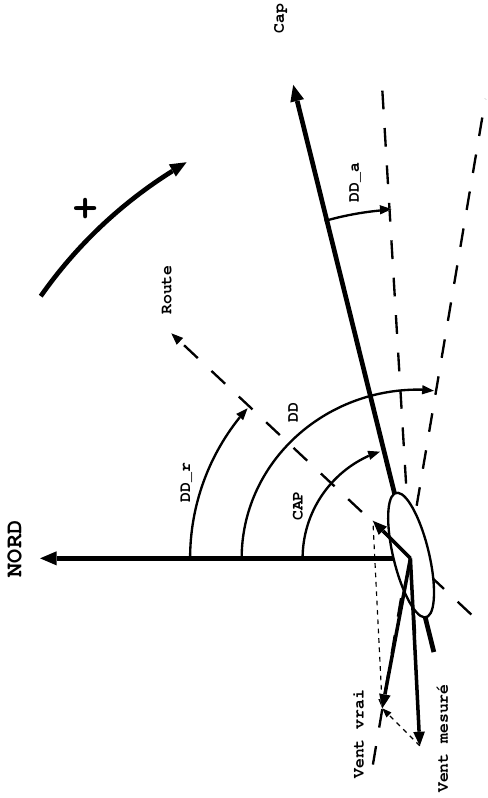
\includegraphics[angle=270,width=0.7\linewidth]{images/graph_arg_vent_bateau_polaire.png}
\end{center}

%%%%%AUTEUR%%%%
\itemstyle{Auteur~:}
CNRM/GMEI/TRAMM

%%%%%REFERENCE%%%%
\itemstyle{R\'ef\'erences~:}


\newpage
%%%%%
%
\section{Composantes horizontales du vent � partir des vitesses dans le 
rep�re mobile}

\itemstyle{Op\'erateur~:} {\sf CalcVent\_h\_repav}
\index{CalcVent\_h\_repav}

%%%%%OBJET%%%%
\itemstyle{Objet~:}
 Calcul simplifi� d'un vent horizontal, � partir
de vitesses exprim�es dans le rep�re d'une plate-forme mobile
(avion, bateau, ...) . Le calcul est
effectu� dans le rep�re li� au mobile, puis une rotation des
composantes les am�ne dans le rep�re g�ographique local (ENU).
Ce calcul n'est valide que lorsque le mobile est horizontal.

%%%%%ARGUMENTS%%%%
\bigskip
%%%%%ENTREES%%%%
\begin{tabarg}
\multicolumn{3}{l}{\titretab {Entr\'ees}}\\
\hline
$V_p$ & Vecteur, {\tt float} & Vitesse propre (m/s)\\
$\beta$ & Vecteur, {\tt float} & Angle de d�rapage, positif lorsque le vent relatif vient de tribord (rad)\\
$\Psi$ & Vecteur, {\tt float} & Cap g�ographique de la plate-forme (rad)\\
$V_x$ & Vecteur, {\tt float} & Vitesse de la plate-forme par rapport au sol, selon l'axe longitudinal dirig� vers l'avant (m/s)\\
$V_y$ & Vecteur, {\tt float} & Vitesse de la plate-forme par rapport au sol selon l'axe transversal dirig� vers de babord vers tribord (m/s)\\
\end{tabarg}

\medskip
%%%%%SORTIES%%%%
\begin{tabarg}
\multicolumn{3}{l}{\titretab {Sorties}}\\
\hline
$U$ & Vecteur, {\tt float} & Composante zonale du vent (Ouest vers Est) (m�me unit� que $V_p$)\\
$V$ & Vecteur, {\tt float} & Composante m�ridienne du vent (Sud au Nord) (m�me unit� que $V_p$)\\
\end{tabarg}


%%%%%FORMULE%%%%
\itemstyle{Formule}

%%CalcVent_h_repav_auto_unit

Dans un premier temps, le vent est calcul\'e dans le rep\`ere li� � la 
plate-forme mobile. Les 2 composantes sont not\'ees $U_a$ et $V_a$.
\begin{eqnarray*}
U_a & = & V_x - V_p.\cos\beta \\
V_a & = & V_y - V_p.\sin\beta 
\end{eqnarray*}

Puis, une rotation permet d'obtenir le 
vent dans le rep\`ere g\'eographique.
\begin{eqnarray*}
U = U_a.\sin\psi + V_a.\cos\psi \\
V = U_a.\cos\psi - V_a.\sin\psi
\end{eqnarray*}


%%%%%AUTEUR%%%%
\itemstyle{Auteur~:}
CNRM/GMEI/TRAMM

%%%%%REFERENCE%%%%
\itemstyle{R\'ef\'erences~:}

\newpage
%%%%%
%
\section{Vent horizontal � partir des vitesses dans le rep�re
mobile (unit�s automatiques)}
%Composantes horizontales du vent � partir des vitesses dans le rep�re
%avion avec reconnaissance de l'unit�}

\itemstyle{Op\'erateur~:} {\sf CalcVent\_h\_repav\_auto\_unit}
\index{CalcVent\_h\_repav\_auto\_unit}

%%%%%OBJET%%%%
\itemstyle{Objet~:}
Calcul simplifi� d'un vent horizontal, � partir
de vitesses exprim�es dans un rep�re li� � une plate-forme mobile. Le
 calcul est effectu� dans le rep�re li� au mobile, puis une rotation des
composantes les am�ne dans le rep�re g�ographique local (ENU).
Ce calcul n'est valide que lorsque le mobile se d�place � plat.\newline
Cet op�rateur travaille avec les diff�rents types d'unit�s dans la
mesure o� celles-ci restent homog�nes. Il faut lui passer en argument
l'unit� de mesure des angles.    

%%%%%ARGUMENTS%%%%
\bigskip
%%%%%ENTREES%%%%
\begin{tabarg}
\multicolumn{3}{l}{\titretab {Entr\'ees}}\\
\hline
$V_p$ & Vecteur, {\tt float} & Vitesse propre ($m/s$ ou $kt$)\\
$\beta$ & Vecteur, {\tt float} & Angle de d�rapage, positif lorsque le vent 
relatif vient de tribord ($radians$ ou $degres$)\\
$\Psi$ & Vecteur, {\tt float} & Cap g�ographique du mobile ($radians$ ou $degres$)\\ 
$unit$  & Coeff., {\tt String         } & Unite de mesure des angles ($radians$
ou $degres$)\\
$V_x$ & Vecteur, {\tt float} & Vitesse du mobile par rapport au sol, sur l'axe 
longitudinal du mobile, dirig� vers l'avant ($m/s$ ou $kt$)\\
$V_y$ & Vecteur, {\tt float} & Vitesse du mobile par rapport au sol, sur l'axe 
transversal du mobile, dirig� vers de babord vers tribord ($m/s$ ou $kt$)\\
\end{tabarg}

\medskip
%%%%%SORTIES%%%%
\begin{tabarg}
\multicolumn{3}{l}{\titretab {Sorties}}\\
\hline
$U$ & Vecteur, {\tt float} & Composante zonale du vent (Ouest vers Est) (m�me unit� que $V_p$)\\
$V$ & Vecteur, {\tt float} & Composante m�ridienne du vent (Sud au Nord) (m�me unit� que $V_p$)\\
\end{tabarg}


%%%%%FORMULE%%%%
\itemstyle{Formule}

%%CalcVent_h_repav_auto_unit

Dans un premier temps, le vent est calcul\'e dans le rep\`ere li� � la 
plate-forme mobile. Les 2 composantes sont not\'ees $U_a$ et $V_a$.
\begin{eqnarray*}
U_a & = & V_x - V_p.\cos\beta \\
V_a & = & V_y - V_p.\sin\beta 
\end{eqnarray*}

Puis, une rotation permet d'obtenir le 
vent dans le rep\`ere g\'eographique.
\begin{eqnarray*}
U = U_a.\sin\psi + V_a.\cos\psi \\
V = U_a.\cos\psi - V_a.\sin\psi
\end{eqnarray*}


%%%%%AUTEUR%%%%
\itemstyle{Auteur~:}
CNRM/GMEI/TRAMM

%%%%%REFERENCE%%%%
\itemstyle{R\'ef\'erences~:}


\newpage
%%%%%
%
%% Dans ce fichier, les �ventuels accents sont cod�s
%% en ISO-8859-15 (aka latin9)
%% La ligne suivante donne trois exemples 
%% e accent aigu : �, e accent grave : �, e-dans-l'o : �
\section{Reconstruction champ de vent}

\itemstyle{Op\'erateur~:} \operfmt{WFR}
\index{WFR}

%%%%%OBJET%%%%
\itemstyle{Objet~:}
Calcul d'un champ de vent \`a partir des profils inclin\'es \`a un angle A de la verticale

%%%%%ARGUMENTS%%%%
\bigskip
%% Dans ce fichier, les �ventuels accents sont cod�s
%% en ISO-8859-15 (aka latin9)
%% La ligne suivante donne trois exemples 
%% e accent aigu : �, e accent grave : �, e-dans-l'o : �
%%%%%ENTREES%%%%
\begin{tabarg}
\multicolumn{3}{l}{\titretab {Entr\'ees}}\\
\hline
$X_1$ & Vecteur, \texttt{float} &  Vecteur 1 de vitesse du vent\\
$X_2$ & Vecteur, \texttt{float} & Vecteur 2 de vitesse du vent\\
$angle$ & Coeff., \texttt{float} & Angle entre la verticale et l'impulsion laser ($^{\circ}$) \\
\end{tabarg}

\medskip
%%%%%SORTIES%%%%
\begin{tabarg}
\multicolumn{3}{l}{\titretab {Sorties}}\\
\hline
$X_{out}$ & Vecteur, \texttt{float} & Champ de vitesse du vent\\
\end{tabarg}


%%%%%FORMULE%%%%
\itemstyle{Formule}

%% Formule de l'operateur : WFR
%% Dans ce fichier, les �ventuels accents sont cod�s
%% en ISO-8859-15 (aka latin9)
%% La ligne suivante donne trois exemples 
%% e accent aigu : �, e accent grave : �, e-dans-l'o : �
\[
u_{i} = \frac{X_{1} - X_{2}}{2*sin(angle)} 
\]



%%%%%AUTEUR%%%%
\itemstyle{Auteur~:}
CNRM/GMEI/TRAMM

%%%%%REFERENCE%%%%
\itemstyle{R\'ef\'erences~:}
WindCube Data Filtering Guidelines (2023).

\newpage
%% THERMODYNAMIQUE %%
%
\section{Humidit\'e relative \`a partir de la sonde carbone}

\itemstyle{ Op\'erateur~: } {\sf HumCarb}
\index{HumCarb}

%%%%%OBJET%%%%%
\itemstyle{ Objet~: }
Cet op\'erateur calcule l'humidit\'e \`a partir de la tension
de la sonde carbone. Il utilise 3 relations diff\'erentes en 
fonction de la temp\'erature (seuils \`a $-10$ et$+12^\circ$C).\newline
Une correction de vitesse est ensuite appliqu\'ee.

%%%%%ARGUMENTS%%%%%
\bigskip
%%%%%ENTREES%%%%/
\begin{tabarg}
\multicolumn{3}{l}{\titretab{Entr\'ees}}\\
\hline
$V$ & Vecteur, \texttt{float} & Tension de la sonde carbone ($V$) \\
$T_s$ & Vecteur, \texttt{float} & Temp\'erature statique de l'air ($K$ ou $^\circ C$) \\
$T_i$ & Vecteur, \texttt{float} & Temp\'erature d'impact ($K$ ou $^\circ C$) \\
$P_s$ & Vecteur, \texttt{float} & Pression statique ($hPa$)\\
$\Delta P$ & Vecteur, \texttt{float} & Pression dynamique ($hPa$)\\
$C_1$ & Coeff., \texttt{float[4]} & Coefficients pour la gamme : $ T_s< -10^\circ C $\\
$C_2$ &  Coeff., \texttt{float[4]} & Coefficients pour la gamme : $ -10^\circ C \leq T_s \leq +12^\circ C $\\
$C_3$ &  Coeff., \texttt{float[4]} & Coefficients pour la gamme : $ +12^\circ C < T_s $\\
\end{tabarg}

\medskip
%%%%%SORTIES%%%%
\begin{tabarg}
\multicolumn{3}{l}{\titretab{Sorties}}\\
\hline
$H_u$ & Vecteur, \texttt{float} & Humidit\'e relative ($\%$)\\
\end{tabarg}


%%%%%FORMULE%%%%
\itemstyle{ Formule }

% calcul de l'humidite carbone
\[
Hu = \frac{ P_s . ew(T_i)}{(P_s + \Delta P) ew(T_s)}
     .\left( C_m[0] + C_m[1].V + C_m[2].V^2 + C_m[3].V^3 + C_m[4].V^4 \right)
\]
$C_m$ est \'egal \`a $C_1$, $C_2$, ou $C_3$ selon la gamme de 
temp\'erature.\newline
$ew()$ est la tension de vapeur saturante par rapport \`a l'eau.
Si $T_s < 0$, $ew()$ est remplac\'ee par la tension de vapeur saturante
par rapport \`a la glace $ewi()$. 


%%%%COMMENTAIRE%%%%
\itemstyle{Commentaire~:}

Les fonctions $ew()$ et $ewi()$ sont d\'ecrites en annexe \ref{annexe-thermo}. 

%%%%%AUTEUR%%%%%
\itemstyle{ Auteur~:}
CNRM/GMEI/TRAMM

%%%%%REFERENCES%%%%%
\itemstyle{ R\'ef\'erences~:}
Note du CAM sur les appareils de mesure de l'hygrom\'etrie \cite{CAM-hum}

\newpage
%% THERMODYNAMIQUE %%
%
\section{Humidit\'e relative \`a partir de la sonde capacitive}

\itemstyle{ Op\'erateur~: } {\sf HumCapa}
\index{HumCapa}

%%%%%OBJET%%%%%
\itemstyle{ Objet~: }
Calcul de l'humidit\'e relative \`a partir de la fr\'equence
mesur\'ee en sortie d'un conditionneur d'une sonde capacitive.

%%%%%ARGUMENTS%%%%%
\bigskip
%%%%%ENTREES%%%%
\begin{tabarg}
\multicolumn{3}{l}{\titretab{ Entr\'ees}}\\
\hline
$Ucapf$ & Vecteur, \texttt{float} & Fr\'equence de sortie de la sonde capacitive ($Hz$) \\
$T_s$ & Vecteur, \texttt{float} & Temp\'erature statique de l'air ($K$ ou $^\circ C$) \\
$P_s$ & Vecteur, \texttt{float} & Pression statique ($hPa$) \\
$\Delta P$ & Vecteur, \texttt{float} & Pression dynamique ($hPa$)\\
$C_t$ & Coeff., \texttt{float} & Coefficient de correction de temp\'erature ($\frac{\%}{^\circ C}$)\\
$Fmin$ & Coeff., \texttt{float} & Fr\'equence minimale acceptable ($Hz$)\\
$C_0$  & Coeff., \texttt{float} & Coefficient de degr\'e 0 de la loi de calibration \\
$C_1$  & Coeff., \texttt{float} & Coefficient de degr\'e 1 de la loi de calibration \\
$C_2$  & Coeff., \texttt{float} & Coefficient de degr\'e 2 de la loi de calibration \\
\end{tabarg}

\medskip
%%%%%SORTIES%%%%
\begin{tabarg}
\multicolumn{3}{l}{\titretab{ Sorties}}\\
\hline
$H_u$ & Vecteur, \texttt{float} & Humidit\'e relative ($\%$)\\
\end{tabarg}


%%%%%FORMULE%%%%
\itemstyle{ Formule }

%%%% THERMODYNAMIQUE
\[
H_u = \frac{P_s}{P_s + \Delta P} \times 
      \left[ C_0 + C_1.Ucapf + C_2.Ucapf^2 + 
       C_t.(T_s - 20 ) \right]
\]
avec $T_s$ exprim\'e en $^\circ C$. \newline
Si $Ucapf \le Fmin$ alors $Ucapf = Fmin $.



%%%%%AUTEUR%%%%%
\itemstyle{ Auteur~:}
CNRM/GMEI/TRAMM

%%%%%REFERENCES%%%%%
\itemstyle{ R\'ef\'erences~:}
Note du CAM sur les appareils de mesure de l'hygrom\'etrie \cite{CAM-hum}.

\newpage
%%%%%
%
\section{Calibration de l'humidit� du capteur aerodata}

\itemstyle{Op\'erateur~:} {\sf Calib\_aerodata\_hum}
\index{Calib\_aerodata\_hum}

%%%%%OBJET%%%%
\itemstyle{Objet~:}
Application de la loi de calibrage aux mesures d'humidit� relative du
capteur aerodata.

%%%%%ARGUMENTS%%%%
\bigskip
%%%%%ENTREES%%%%
\begin{tabarg}
\multicolumn{3}{l}{\titretab {Entr\'ees}}\\
\hline
$RH_{brut}$ & Vecteur, \texttt{float} & Humidit� relative non calibr�e (\%)\\
$TRT$ & Vecteur, \texttt{float} & Temp�rature d'impact (Celsius ou Kelvin)\\
$a_1$ & Coeff., \texttt{float} & coefficient de calibration\\
$a_2$ & Coeff., \texttt{float} & coefficient de calibration\\
$a_3$ & Coeff., \texttt{float} & coefficient de calibration\\
$a_4$ & Coeff., \texttt{float} & coefficient de calibration\\
$b_1$ & Coeff., \texttt{float} & coefficient de calibration\\
$b_2$ & Coeff., \texttt{float} & coefficient de calibration\\
$b_3$ & Coeff., \texttt{float} & coefficient de calibration\\
$b_4$ & Coeff., \texttt{float} & coefficient de calibration\\
\end{tabarg}

\medskip
%%%%%SORTIES%%%%
\begin{tabarg}
\multicolumn{3}{l}{\titretab {Sorties}}\\
\hline
$RH$ & Vecteur, \texttt{float} & Humidit� relative calibr�e (\%)\\
\end{tabarg}


%%%%%FORMULE%%%%
\itemstyle{Formule}

%%  Calib_aerodata_hum
Si besoin est, $TRT$ est converti en Kelvin, puis :
\[
RH = \left(b_2 + 
      \frac{b_1 - b_2}{1 + \left(\frac{TRT + 50 }{b_3}\right)^{b_4}}
     \right)
  RH_{brut}
+ \left(a_2 + 
      \frac{a_1 - a_2}{1 + \left(\frac{TRT + 50 }{a_3}\right)^{a_4}}
     \right)
\]



%%%%%AUTEUR%%%%
\itemstyle{Auteur~:}
CNRM/GMEI/TRAMM

%%%%%REFERENCE%%%%
\itemstyle{R\'ef\'erences~:}
Application d'une loi indiqu�e par Manfred Helten
� P. Nedelec, dans un e-mail du 13 oct 2000.


\newpage
%%%%%
%
\section{Humidit\'e relative \`a partir de la sonde capacitive}

\itemstyle{Op\'erateur~:} {\sf HumEmpir}
\index{HumEmpir}

%%%%%OBJET%%%%
\itemstyle{Objet~:}
Calcul de l'humidit\'e relative \`a partir d'une 
sonde capacitive, en utilisant une loi
de calibration empirique compos\'e de 2 fonctions
lin\'eaires.

%%%%%ARGUMENTS%%%%
\bigskip
%%%%%ENTREES%%%%
\begin{tabarg}
\multicolumn{3}{l}{\titretab {Entr\'ees}}\\
\hline
$T_s$ & Vecteur, {\tt float} & Temp\'erature de l'air ($K$)\\
$T_t$ & Vecteur, {\tt float} & Temp\'erature totale ($K$)\\
$V$ & Vecteur, {\tt float} & Tension de sortie de la sonde ($V$)\\
$P_s$ & Vecteur, {\tt float} & Pression statique ($hPa$)\\
$\Delta P$ & Vecteur, {\tt float} & Pression dynamique ($hPa$)\\
$C$ & Coeff., {\tt float[5]} & Coefficients de calibration \\ 
\end{tabarg}

\medskip
%%%%%SORTIES%%%%
\begin{tabarg}
\multicolumn{3}{l}{\titretab {Sorties}}\\
\hline
$H_u$ & Vecteur, {\tt float} & Humidit\'e relative (\%)\\
\end{tabarg}


%%%%%FORMULE%%%%
\itemstyle{Formule}

%%HumEmpir
Si $V \le C[0]$ alors \\ 
$$ 
X = C[1] + C[2].V 
$$
sinon \\ 
$$ 
X = C[3] + C[4].V 
$$ \\
et 
$$
H_u = \frac{P_s}{P_s + \Delta P} \times 
      \frac{ew(T_t)}{ew(T_s)}
      \left[ X + 
       0.075 \times (293.16 - T_s) \right] \\
$$
avec $T_s$ exprim\'e en $K$.


%%%%COMMENTAIRE%%%%
\itemstyle{Commentaire~:}

Les fonctions $ew()$ et $ewi()$ sont d\'ecrites en annexe
\ref{annexe-thermo}.

%%%%%AUTEUR%%%%
\itemstyle{Auteur~:}
CNRM/GMEI/TRAMM

%%%%%REFERENCE%%%%
\itemstyle{R\'ef\'erences~:}

\newpage
%%%%%
%
%% Dans ce fichier, les �ventuels accents sont cod�s
%% en ISO-8859-15 (aka latin9)
%% La ligne suivante donne trois exemples 
%% e accent aigu : �, e accent grave : �, e-dans-l'o : �
\section{Humidit� relative en fonction de l'Humidit� Sp�cifique}

\itemstyle{Op\'erateur~:} \operfmt{Humrel\_Humspec}
\index{Humrel\_Humspec}

%%%%%OBJET%%%%
\itemstyle{Objet~:}
Calcul de l'humidit� relative en fonction de l'humidit� sp�cifique et des param�tres d'�tat temp�rature et pression statique.

%%%%%ARGUMENTS%%%%
\bigskip
%% Dans ce fichier, les �ventuels accents sont cod�s
%% en ISO-8859-15 (aka latin9)
%% La ligne suivante donne trois exemples 
%% e accent aigu : �, e accent grave : �, e-dans-l'o : �
%%%%%ENTREES%%%%
\begin{tabarg}
\multicolumn{3}{l}{\titretab {Entr\'ees}}\\
\hline
SH & Vecteur, \texttt{float} & Humidit�  sp�cifique (g/kg)\\
$P_s$ & Vecteur, \texttt{float} & Pression statique (hPa)\\
T & Vecteur, \texttt{float} & Temp�rature de l'air(Kelvin)\\
\end{tabarg}

\medskip
%%%%%SORTIES%%%%
\begin{tabarg}
\multicolumn{3}{l}{\titretab {Sorties}}\\
\hline
RH & Vecteur, \texttt{float} & Humidit� relative (percent)\\
\end{tabarg}


%%%%%FORMULE%%%%
\itemstyle{Formule}

%% Formule de l'operateur : Humrel_Humspec
%\[
Humidit� sp�cifique � saturation en g/kg:
\[
Q_s = \frac{SH}{1000.} 
\]

Pression de vapeur: 
\[
E_s = \frac{Q_s  \times P_s} {\frac{R_a}{R_v} + Q_s \times \frac{1-R_a}{R_v}}
\]
avec    
\[
    R_a= \frac{8.314510}  {0.028964} 
\]
et
\[
R_v=461.51
\]
 
Calcul de la tension de vapeur saturante en fonction de $T0$=273.15�K

\[
\begin{tabular}{lll}
    \text{Si} T > $T0$ \text{alors} &ewt= ew(T) & \text{la tension de vapeur saturante de l'eau} \\

    \text{sinon}& ewt=ewi(T) & \text{la tension de vapeur saturante de la glace} 
\end{tabular}
\]

Calcul de humidit� relative:

\[
RH = \frac{100 \times E_s }{ ewt}
\]

%\]



%%%%COMMENTAIRE%%%%
\itemstyle{Commentaire~:}
Les fonctions $ew()$ et $ewi()$ sont d\'ecrites en annexe
\ref{annexe-thermo}.


%%%%%AUTEUR%%%%
\itemstyle{Auteur~:}
CNRM/GMEI/TRAMM

%%%%%REFERENCE%%%%
\itemstyle{R\'ef\'erences~:}


\newpage
%%%%%
%
\section{Correction de vitesse sur l'humidit� relative}

\itemstyle{Op\'erateur~:} \operfmt{Calc\_Static\_RH\_From\_Dynamic\_RH\_V1}
\label{OP-Calc_Static_RH_From_Dynamic_RH_V1}
\index{Calc\_Static\_RH\_From\_Dynamic\_RH\_V1}

%%%%%OBJET%%%%
\itemstyle{Objet~:}
Correction des effets de compression et de
r�chauffement qui affectent la mesure d'humidit� relative
sur plate-forme mobiles.

%%%%%ARGUMENTS%%%%
\bigskip
%%%%%ENTREES%%%%
\begin{tabarg}
\multicolumn{3}{l}{\titretab {Entr\'ees}}\\
\hline
$HU_{dyn}$ & Vecteur, \texttt{float} & Mesure d'humidit� relative dans des
conditions de vitesse/surpression (\%)\\
$T_s$ & Vecteur, \texttt{float} & Temp�rature statique de l'air (�C ou K)\\
$T_t$ & Vecteur, \texttt{float} & Temp�rature totale (�C ou K)\\
\end{tabarg}

\medskip
%%%%%SORTIES%%%%
\begin{tabarg}
\multicolumn{3}{l}{\titretab {Sorties}}\\
\hline
$HU_{stat}$ & Vecteur, \texttt{float} & Humidit� relative corrig�e des effets de 
la vitesse (\%)\\
\end{tabarg}


%%%%%FORMULE%%%%
\itemstyle{Formule}

%% Calc_Static_RH_From_Dynamic_RH_V1
Si besoin est, $T_s$ et $T_t$ sont convertis en kelvins, puis
\[
HU_{stat} = 
\frac{e_w(T_t)}{e_w(T_s)}
\left(\frac{T_s}{T_t}\right)^{\frac{\gamma}{\gamma-1}}
% \gamma = 1005./717.
HU_{dyn}
\]
avec $\gamma =  1005/717 = 1.40167364$


%%%%%AUTEUR%%%%
\itemstyle{Auteur~:}
Le programme originel �tait �crit en Pascal, et nous a �t�
transmis par M. Helten (Research centre Juelich GmbH). La version
en C, aussi fid�le que possible � l'original, a �t� �crite par B. Piguet.

%%%%%REFERENCE%%%%
\itemstyle{R\'ef\'erences~:}
La tension de vapeur saturante est calcul�e avec
les formules 3.17 et 3.18 donn�es dans Sonntag (1982)
% : Formula 3.17 & 3.18
%  with regards to Liquid Water and Ice respectivily.


\newpage
%%%%%
%
\section{Simulation d'effet de vitesse sur l'humidit� relative}

\itemstyle{Op\'erateur~:} \operfmt{Dynamic\_RH\_from\_static}
\label{OP-Dynamic_RH_from_static}
\index{Dynamic\_RH\_from\_static}

%%%%%OBJET%%%%
\itemstyle{Objet~:}
Calcul d'une humidit� relative affect�e par les effets de compression et de 
r�chauffement qui se produisent en fonction de la vitesse,
� partir d'une humidit� non-perturb�e ("statique" ou "infinie-amont"), et
des temp�ratures statiques/totales correspondant au r�chauffement
adiabatique induit par la vitesse.

%%%%%ARGUMENTS%%%%
\bigskip
%%%%%ENTREES%%%%
\begin{tabarg}
\multicolumn{3}{l}{\titretab {Entr\'ees}}\\
\hline
$HU_{stat}$ & Vecteur, \texttt{float} & Humidit� relative (\%) \\
$T_s$ & Vecteur, \texttt{float} & Temp�rature statique de l'air (�C ou K)\\
$T_t$ & Vecteur, \texttt{float} & Temp�rature totale (�C ou K)\\
\end{tabarg}

\medskip
%%%%%SORTIES%%%%
\begin{tabarg}
\multicolumn{3}{l}{\titretab {Sorties}}\\
\hline
$HU_{dyn}$ & Vecteur, \texttt{float} & Humidit� relative dans les
conditions de vitesse/surpression correspondant � un r�chauffement
adiabatique produisant $T_t$ (\%)\\
\end{tabarg}


%%%%%FORMULE%%%%
\itemstyle{Formule}

%% Dynamic_RH_from_static
\[
HU_{dyn} = 
\frac{e_w(T_s)}{e_w(T_t)}
\left(\left(\frac{T_s}{T_t}\right)^{\frac{\gamma}{\gamma-1}}\right)^{-1}
HU_{stat}
\]
avec $\gamma =  1005/717 = 1.40167364$


%%%%%AUTEUR%%%%
\itemstyle{Auteur~:}
CNRM/GMEI/TRAMM

%%%%%REFERENCE%%%%
\itemstyle{R\'ef\'erences~:}
Cette fonction est la r�cipoque de 
\hyperref[OP-Calc_Static_RH_From_Dynamic_RH_V1]{\operfmt{Calc\_Static\_RH\_From\_Dynamic\_RH\_V1}}

\newpage
%%%%%
%
%% Dans ce fichier, les �ventuels accents sont cod�s
%% en ISO-8859-15 (aka latin9)
%% La ligne suivante donne trois exemples 
%% e accent aigu : �, e accent grave : �, e-dans-l'o : �
\section{Correction de l'influence de la pression sur la mesure de Tdf}

\itemstyle{Op�rateur~:} \operfmt{Correc\_Tdf\_P}
\index{Correc\_Tdf\_P}

%%%%%OBJET%%%%
\itemstyle{Objet~:}
 Toute variation de pression d'une parcelle d'air change
proportionnellement la pression partielle de vapeur d'eau,
et donc la valeur du point de ros�e (ou de givre), qui
est la temp�rature telle que ewt(Td) = e.

Cet op�rateur corrige les mesures de Td/Tf faites � une pression
diff�rente de celle de l'air qu'on souhaite caract�riser.

%%%%%ARGUMENTS%%%%
\bigskip
%% Dans ce fichier, les �ventuels accents sont cod�s
%% en ISO-8859-15 (aka latin9)
%% La ligne suivante donne trois exemples 
%% e accent aigu : �, e accent grave : �, e-dans-l'o : �
%%%%%ENTREES%%%%
\begin{tabarg}
\multicolumn{3}{l}{\titretab {Entr\'ees}}\\
\hline
$Tdf_m$ & Vecteur, \texttt{float} &  Temp�rature de ros�e ou givre mesur�e (�C ou K)\\
$Ps_m$ & Vecteur, \texttt{float} & Pression de mesure (hPa)\\
$Ps$ & Vecteur, \texttt{float} & Pression de l'air (m�me unit� que $Ps_m$)\\
\end{tabarg}

\medskip
%%%%%SORTIES%%%%
\begin{tabarg}
\multicolumn{3}{l}{\titretab {Sorties}}\\
\hline
$Tdf$ & Vecteur, \texttt{float} & Temp�rature de ros�e ou givre corrig�e (m�me
unit� que $Tdf_m$)\\
\end{tabarg}


%%%%%FORMULE%%%%
\itemstyle{Formule}

%% Formule de l'operateur : Correc_Tdf_P
%% Dans ce fichier, les �ventuels accents sont cod�s
%% en ISO-8859-15 (aka latin9)
%% La ligne suivante donne trois exemples 
%% e accent aigu : �, e accent grave : �, e-dans-l'o : �
\[
Tdf = ew^{-1} (ew(Td_m) \frac{P}{P_m})
\]



%%%%%AUTEUR%%%%
\itemstyle{Auteur~:}
CNRM/GMEI/TRAMM

%%%%%REFERENCE%%%%
\itemstyle{R\'ef\'erences~:}
%INCONNU

\newpage
%% THERMODYNAMIQUE %%
%
\section{Humidit� relative � partir de la temp�rature du point
de ros�e, seuill�e � 101\%}

\itemstyle{ Op�rateur~: } \operfmt{HumW\_T\_Td}
\index{HumW\_T\_Td}

%%%%%OBJET%%%%%
\itemstyle{ Objet~: }
Cet op�rateur calcule l'humidit� relative � l'eau liquide � partir
des temp�ratures de l'air et du point de ros�e.

%%%%%ARGUMENTS%%%%%
\bigskip
%%%%%ENTREES%%%%
\begin{tabarg}
\multicolumn{3}{l}{\titretab{ Entr\'ees}}\\
\hline
$T_s$ & Vecteur, \texttt{float} & Temp\'erature statique de l'air ($K$ ou $^\circ C$) \\
$T_d$ & Vecteur, \texttt{float} & Temp\'erature du point de ros\'ee ($K$ ou $^\circ C$) 
\end{tabarg}

\medskip
%%%%%SORTIES%%%%
\begin{tabarg}
\multicolumn{3}{l}{\titretab{Sorties}}\\
\hline
$H_u$ & Vecteur, \texttt{float} & Humidit\'e relative \`a l'eau liquide ($\%$)\\
\end{tabarg}


%%%%%FORMULE%%%%
\itemstyle{ Formule }

%%%% THERMODYNAMIQUE
\[
H_u = 100 \times \frac{ e_w(T_d)}{e_w(T_s)} 
\]
Si $T_d > T_s$ alors $H_u$ est forc\'e \`a 101\%.



%%%%COMMENTAIRE%%%%
\itemstyle{Commentaire~:}

La fonction $ew()$ est d�crite en annexe
\ref{annexe-thermo}.

Les formules employ�es correspondent � l'hypoth�se que 
l'argument d'entr�e $T_d$ est toujours un point de ros�e (et non
un point de givre si $T_d < 0$�C); 
si $T_d$ provient d'un calcul, cette hypoth�se peut �tre v�rifi�e,
mais si il provient d'un hygrom�tre � miroir
refroidi, il est probable que les valeurs en-dessous de 0�C soient
une mesure de point de givre, et il vaut mieux utiliser l'op�rateur
\hyperref[OP-HumW_T_Tdf]{\operfmt{HumW\_T\_Tdf}}.


%%%%%AUTEUR%%%%%
\itemstyle{ Auteur~:}
CNRM/GMEI/TRAMM

%%%%%REFERENCES%%%%%
\itemstyle{ R�f�rences~:}

\emph{M�t�orologie G�n�rale}, Triplet-Roche, �dition de 1971\cite{Triplet-Roche}, p59.

\newpage
%% THERMODYNAMIQUE %%
%
\section{Humidit\'e relative \`a partir de la temp\'erature du point
de ros\'ee sans seuillage}

\itemstyle{ Op\'erateur~: } {\sf HumW\_T\_Td\_no\_limit}
\index{HumW\_T\_Td\_no\_limit}

%%%%%OBJET%%%%%
\itemstyle{ Objet~: }
Cet op\'erateur calcule l'humidit\'e \`a partir de la temp\'erature 
du point de ros\'ee et de la temp\'erature de l'air, en utilisant les
formules relatives \`a l'eau liquide. 

%%%%%ARGUMENTS%%%%%
\bigskip
%%%%%ENTREES%%%%
\begin{tabarg}
\multicolumn{3}{l}{\titretab{ Entr\'ees}}\\
\hline
$T_s$ & Vecteur, {\tt float} & Temp\'erature statique de l'air ($K$ ou $^\circ C$) \\
$T_d$ & Vecteur, {\tt float} & Temp\'erature du point de ros\'ee ($K$ ou $^\circ C$) 
\end{tabarg}

\medskip
%%%%%SORTIES%%%%
\begin{tabarg}
\multicolumn{3}{l}{\titretab{Sorties}}\\
\hline
$H_u$ & Vecteur, {\tt float} & Humidit\'e relative ($\%$)\\
\end{tabarg}


%%%%%FORMULE%%%%
\itemstyle{ Formule }

%%%% THERMODYNAMIQUE
\[
H_u = 100 \times \frac{ e_w(T_d)}{e_w(T_s)} 
\]



%%%%COMMENTAIRE%%%%
\itemstyle{Commentaire~:}

La fonction $ew()$ est d\'ecrite en annexe
\ref{annexe-thermo}.

%%%%%AUTEUR%%%%%
\itemstyle{ Auteur~:}
CNRM/CAM/ITD

%%%%%REFERENCES%%%%%
\itemstyle{ R\'ef\'erences~:}
Triplet-Roche \cite{Triplet-Roche}

\newpage
%%%%%
%
%% Dans ce fichier, les �ventuels accents sont cod�s
%% en ISO-8859-15 (aka latin9)
%% La ligne suivante donne trois exemples 
%% e accent aigu : �, e accent grave : �, e-dans-l'o : 1/2

\section[Humidit� relative � partir du point de ros�e ou de givre,
seuill�e � 102\%]{Humidit� relative � partir de la temp�rature
du point de ros�e ou de givre, seuill�e � 102\%}

\itemstyle{Op�rateur~:} \operfmt{HumW\_T\_Tdf}
\label{OP-HumW_T_Tdf}
\index{HumW\_T\_Tdf}

%%%%%OBJET%%%%%
\itemstyle{ Objet~: }
Cet op�rateur calcule l'humidit� relative � l'eau liquide � partir de la
temp�rature 
du point de ros�e ou de givre et de la temp�rature de l'air.

%%%%%ARGUMENTS%%%%
\bigskip
%% Dans ce fichier, les �ventuels accents sont cod�s
%% en ISO-8859-15 (aka latin9)
%% La ligne suivante donne trois exemples 
%% e accent aigu : �, e accent grave : �, e-dans-l'o : 1/2
%%%%%ENTREES%%%%
\begin{tabarg}
\multicolumn{3}{l}{\titretab {Entr�es}}\\
\hline
$T_s$ & Vecteur, \texttt{float} & Temp�rature de l'air ($K$ ou $^\circ C$) \\
$T_{df}$ & Vecteur, \texttt{float} & Temp�rature du point de ros�e ou de givre ($K$ ou $^\circ C$) 
\end{tabarg}

\medskip
%%%%%SORTIES%%%%
\begin{tabarg}
\multicolumn{3}{l}{\titretab {Sorties}}\\
\hline
$H_u$ & Vecteur, \texttt{float} & Humidit� relative � l'eau liquide (\%)\\
\end{tabarg}


%%%%%FORMULE%%%%
\itemstyle{Formule}

%% Formule de l'operateur : HumW_T_Tdf
%% Dans ce fichier, les �ventuels accents sont cod�s
%% en ISO-8859-15 (aka latin9)
%% La ligne suivante donne trois exemples 
%% e accent aigu : �, e accent grave : �, e-dans-l'o : �
\[
e = 
\begin{cases}
 e_w(T_{df}) \text{ si } T_{df} \ge 0.0 \text{�C}\\
 e_{wi}(T_{df}) \text{ sinon}\\
\end{cases}
H_u = 100 \times \frac{e}{e_w(T_s)} 
\]
Si $H_u > 102 \%$, $Hu = 103 \%$.


%%%%COMMENTAIRE%%%%
\itemstyle{Commentaire~:}

Les fonctions $ew()$ et  $ewi()$ sont d\'ecrites en annexe
\ref{annexe-thermo}.

%%%%%AUTEUR%%%%
\itemstyle{Auteur~:}
CNRM/GMEI/TRAMM

%%%%%REFERENCE%%%%
\itemstyle{R�f�rences~:}

\emph{M�t�orologie G�n�rale}, Triplet-Roche, �dition de 1971\cite{Triplet-Roche}, p59.

\newpage
%%%%%
%
\section{Humidit� relative � la glace � partir de T et Td}

\itemstyle{Op\'erateur~:} \textsf{HumI\_T\_Td}
\index{HumI\_T\_Td}

%%%%%OBJET%%%%
\itemstyle{Objet~:}
Calcule l'humidit� relative \`a partir de la temp\'erature 
du point de ros\'ee et de la temp\'erature de l'air, en utilisant les
formules relatives \`a la glace. 

%%%%%ARGUMENTS%%%%
\bigskip
%%%%%ENTREES%%%%
\begin{tabarg}
\multicolumn{3}{l}{\titretab{ Entr\'ees}}\\
\hline
$T_s$ & Vecteur, \texttt{float} & Temp\'erature statique de l'air ($K$ ou $^\circ C$) \\
$T_d$ & Vecteur, \texttt{float} & Temp\'erature du point de ros\'ee ($K$ ou $^\circ C$) 
\end{tabarg}

\medskip
%%%%%SORTIES%%%%
\begin{tabarg}
\multicolumn{3}{l}{\titretab{Sorties}}\\
\hline
$H_u$ & Vecteur, \texttt{float} & Humidit\'e relative � la glace ($\%$)\\
\end{tabarg}


%%%%%FORMULE%%%%
\itemstyle{Formule}

%%%% THERMODYNAMIQUE
\[
H_u = 100 \times \frac{e_w(T_d)}{e_{wi}(T_s)} 
\]
Si $H_u > 115 \%$, $Hu = 115 \%$.



%%%%COMMENTAIRE%%%%
\itemstyle{Commentaire~:}

Les fonctions $ew()$ et  $ewi()$ sont d\'ecrites en annexe
\ref{annexe-thermo}.

Pour les mesures m�t�orologiques op�rationnelles (par exemple
les radiosondages), l'humidit� relative est toujours d�finie
par rapport � l'eau liquide, m�me � des temp�ratures
inf�rieures � 0�C (cf. le \emph{Guide des instruments et des m�thodes
d'observation m�t�orologique} \cite{OMM-N8-1996}). Le r�sultat
de cet op�rateur ne peut donc pas �tre directement 
compar� � de telles mesures.

%%%%%AUTEUR%%%%
\itemstyle{Auteur~:}
CNRM/GMEI/TRAMM

%%%%%REFERENCE%%%%
\itemstyle{R\'ef\'erences~:}

\newpage
%%%%%
%
\section{Humidit� relative � partir du rapport de m�lange en vapeur d'eau }

\itemstyle{Op\'erateur~:} {\sf Hu\_RapM}
\index{Hu\_RapM}

%%%%%OBJET%%%%
\itemstyle{Objet~:}
 Calcul d'une humidit� relative � partir d'un rapport de m�lange
en vapeur d'eau et des param�tres d'�tat (Pression, temp�rature).

Comme pour la fonction sym�trique ({\sf RapM\_Hu}), le calcul de la tension
de vapeur saturante ($ew(T)$)
se fait TOUJOURS par rapport � de l'eau liquide.

%%%%%ARGUMENTS%%%%
\bigskip
%%%%%ENTREES%%%%
\begin{tabarg}
\multicolumn{3}{l}{\titretab {Entr\'ees}}\\
\hline
$RapM$ & Vecteur, \texttt{float} & Rapport de m�lange (g/kg)\\
$T_s$ & Vecteur, \texttt{float} & Temp�rature (K ou $^\circ$C)\\
$P_s$ & Vecteur, \texttt{float} & Pression (hPa)\\
\end{tabarg}

\medskip
%%%%%SORTIES%%%%
\begin{tabarg}
\multicolumn{3}{l}{\titretab {Sorties}}\\
\hline
$Hum$ & Vecteur, \texttt{float} & Humidit� relative (\%)\\
\end{tabarg}


%%%%%FORMULE%%%%
\itemstyle{Formule}

%%Hu_RapM
\[
e = P . \frac{RapM}{( RapM + 622. )}
\]
\[
Hum = \frac{100}{e_w(T_s)}
\]



%%%%%AUTEUR%%%%
\itemstyle{Auteur~:}
CNRM/GMEI/TRAMM

%%%%%REFERENCE%%%%
\itemstyle{R\'ef\'erences~:}
Triplet-Roche%%\cite{}

\newpage
%%%%%
%
\section{Humidit� relative � partir de l'humidit� absolue}

\itemstyle{Op\'erateur~:} {\sf Hu\_Ha}
\index{Hu\_Ha}

%%%%%OBJET%%%%
\itemstyle{Objet~:}
Calcul de l'humidit� relative � partir de l'humidit� absolue (rapport
de la masse de vapeur $m_v$ au volume $V$ occup� par le m�lange : 
$m_v$/$V$) et de la temp�rature d'�tat de l'air.

%%%%%ARGUMENTS%%%%
\bigskip
%%%%%ENTREES%%%%
\begin{tabarg}
\multicolumn{3}{l}{\titretab {Entr\'ees}}\\
\hline
$T_{s}$ & Vecteur, \texttt{float} & Temp�rature de l'air (Kelvin ou degr�s Celsius)\\
$H_{a}$ & Vecteur, \texttt{float} & Humidit� absolue ($g/m^3$)\\
\end{tabarg}

\medskip
%%%%%SORTIES%%%%
\begin{tabarg}
\multicolumn{3}{l}{\titretab {Sorties}}\\
\hline
$H_u$ & Vecteur, \texttt{float} & Humidit� relative ( \% )\\
\end{tabarg}


%%%%%FORMULE%%%%
\itemstyle{Formule}

%% Hu_Ha
Si besoin est, $T_{s}$ est converti en Kelvin, puis :
\[
e = \frac{H_{a}}{1000} R_v T_{s}
\]
\[
H_{u} = 100 \frac{e}{e_{w}(T_{s})}
\]
Avec :\newline
$R_v = 461.51 J kg^{-1} K^{-1}$ (constante sp�cifique de la vapeur d'eau).\newline
La fonction $e_w(T)$ (tension de vapeur saturante au-dessus de l'eau liquide)
est celle de la biblioth�que thermodynamique d'AIDA, d�crite en annexe 
\ref{annexe-thermo-ew}.


%%%%%AUTEUR%%%%
\itemstyle{Auteur~:}
CNRM/GMEI/TRAMM

%%%%%REFERENCE%%%%
\itemstyle{R\'ef\'erences~:}

\newpage
%%%%%
%
%% Dans ce fichier, les �ventuels accents sont cod�s
%% en ISO-8859-15 (aka latin9)
%% La ligne suivante donne trois exemples 
%% e accent aigu : �, e accent grave : �, e-dans-l'o : �
\section{Humidit� relative � la glace � partir de l'humidit� relative � l'eau liquide}

\itemstyle{Op�rateur~:} \operfmt{Hui\_Hu}
\index{Hui\_Hu}

%%%%%OBJET%%%%
\itemstyle{Objet~:}
Calcul de l'humidit� relative � la glace � partir de
l'humidit� relative � l'eau liquide et de la temp�rature.

%%%%%ARGUMENTS%%%%
\bigskip
%% Dans ce fichier, les �ventuels accents sont cod�s
%% en ISO-8859-15 (aka latin9)
%% La ligne suivante donne trois exemples 
%% e accent aigu : �, e accent grave : �, e-dans-l'o : �
%%%%%ENTREES%%%%
\begin{tabarg}
\multicolumn{3}{l}{\titretab {Entr\'ees}}\\
\hline
$T$ & Vecteur, \texttt{float} & Temp�rature de l'air (K ou �C)\\
$Hu$ & Vecteur, \texttt{float} & Humidit� relative � l'eau liquide (\%)\\
\end{tabarg}

\medskip
%%%%%SORTIES%%%%
\begin{tabarg}
\multicolumn{3}{l}{\titretab {Sorties}}\\
\hline
$Hui$ & Vecteur, \texttt{float} & Humidit� relative � la glace (\%)\\
\end{tabarg}


%%%%%FORMULE%%%%
\itemstyle{Formule}

%% Formule de l'operateur : Hui_Hu
%% Dans ce fichier, les �ventuels accents sont cod�s
%% en ISO-8859-15 (aka latin9)
%% La ligne suivante donne trois exemples 
%% e accent aigu : �, e accent grave : �, e-dans-l'o : �
Si $T < O \text{�C}$
\[
Hui = Hu \frac{ew(T)}{ewi(T)}
\]


%%%%%AUTEUR%%%%
\itemstyle{Auteur~:}
CNRM/GMEI/TRAMM

%%%%%REFERENCE%%%%
\itemstyle{R\'ef\'erences~:}

\newpage
%%%%%
%
\section{Humidit� relative � la glace � partir de l'humidit� absolue}

\itemstyle{Op\'erateur~:} \textsf{Hui\_Ha}
\index{Hui\_Ha}

%%%%%OBJET%%%%
\itemstyle{Objet~:}
Calcul de l'humidit� relative � la glace, � partir de l'humidit� absolue 
(rapport de la masse de vapeur $m_v$ au volume $V$ occup� par le m�lange : 
$m_v$/$V$) et de la temp�rature d'�tat de l'air.

%%%%%ARGUMENTS%%%%
\bigskip
%%%%%ENTREES%%%%
\begin{tabarg}
\multicolumn{3}{l}{\titretab {Entr\'ees}}\\
\hline
$T_{s}$ & Vecteur, \texttt{float} & Temp�rature de l'air (Kelvin ou degr�s Celsius)\\
$H_{a}$ & Vecteur, \texttt{float} & Humidit� absolue ($g/m^3$)\\
\end{tabarg}

\medskip
%%%%%SORTIES%%%%
\begin{tabarg}
\multicolumn{3}{l}{\titretab {Sorties}}\\
\hline
$H_u$ & Vecteur, \texttt{float} & Humidit� relative � la glace ( \% )\\
\end{tabarg}


%%%%%FORMULE%%%%
\itemstyle{Formule}

%% Hui_Ha
Si besoin est, $T_{s}$ est converti en Kelvin, puis :
\[
e = \frac{H_{a}}{1000} R_v T_{s}
\]
\[
H_{u} = 100 \frac{e}{e_{wi}(T_{s})}
\]
Avec :\newline
$R_v = 461.51 J kg^{-1} K^{-1}$ (constante sp�cifique de la vapeur d'eau).\newline
La fonction $e_{wi}(T)$ (tension de vapeur saturante au-dessus de la glace) est celle de la biblioth�que thermodynamique d'AIDA, d�crite en annexe \ref{annexe-thermo-ewi}.



%%%%%AUTEUR%%%%
\itemstyle{Auteur~:}
CNRM/GMEI/TRAMM

%%%%%REFERENCE%%%%
\itemstyle{R\'ef\'erences~:}

\newpage
%%%%%
%
\section{Humidit� absolue � partir de relative}

\itemstyle{Op\'erateur~:} \operfmt{Ha\_Hu}
\index{Ha\_Hu}

%%%%%OBJET%%%%
\itemstyle{Objet~:}
Calcul d'une humidit� absolue (ou volumique), exprim�e en masse de
vapeur d'eau par volume d'air humide, � partir de l'humidit�
relative et de la temp�rature.

%%%%%ARGUMENTS%%%%
\bigskip
%%%%%ENTREES%%%%
\begin{tabarg}
\multicolumn{3}{l}{\titretab {Entr\'ees}}\\
\hline
T & Vecteur, \texttt{float} & Temp�rature de l'air (�C ou Kelvin)\\
Hu & Vecteur, \texttt{float} & Humidit� relative (\%)\\
\end{tabarg}

\medskip
%%%%%SORTIES%%%%
\begin{tabarg}
\multicolumn{3}{l}{\titretab {Sorties}}\\
\hline
Ha & Vecteur, \texttt{float} & Humidit� absolue ( gram/m$^{3}$ )\\
\end{tabarg}


%%%%%FORMULE%%%%
\itemstyle{Formule}

%%Ha_Hu
T est converti en Kelvin, si besoin est, puis :
\[
\text{Ha} = 1000  \frac{\frac{\text{Hu}}{100} . e_{w}(T)}{ R_v . T}
\]
avec :\newline
$R_v$ = 461.51  J kg$^{-1}$ K$^{-1}$ (constante sp�cifique de la vapeur d'eau).\newline
La fonction $e_w(T)$ (tension de vapeur saturante au-dessus de l'eau liquide)
est celle de la biblioth�que thermodynamique d'AIDA, d�crite en annexe 
\ref{annexe-thermo-ew}.


%%%%%AUTEUR%%%%
\itemstyle{Auteur~:}
CNRM/GMEI/TRAMM

%%%%%REFERENCE%%%%
\itemstyle{R\'ef\'erences~:}

\newpage
%%%%%
%
\section{Humidit� absolue � partir du rapport de m�lange}

\itemstyle{Op\'erateur~:} \operfmt{ Ha\_RapM}
\index{Ha\_RapM}

%%%%%OBJET%%%%
\itemstyle{Objet~:}
Calcul de l'humidit� absolue (g/m$^3$) � partir du rapport
de m�lange en vapeur d'eau (g/kg) et des param�tre d'�tat
de l'air (P, T).

%%%%%ARGUMENTS%%%%
\bigskip
%%%%%ENTREES%%%%
\begin{tabarg}
\multicolumn{3}{l}{\titretab {Entr\'ees}}\\
\hline
$r_g$ & Vecteur, \texttt{float} & Rapport de m�lange (gram/kg)\\
$P_{s}$ & Vecteur, \texttt{float} & Pression de l'air (hPa)\\
$T_{s}$ & Vecteur, \texttt{float} & Temp�rature de l'air (K ou �C)\\
\end{tabarg}

\medskip
%%%%%SORTIES%%%%
\begin{tabarg}
\multicolumn{3}{l}{\titretab {Sorties}}\\
\hline
$Ha$ & Vecteur, \texttt{float} & Humidit� absolue (gram/m$^3$)\\
\end{tabarg}


%%%%%FORMULE%%%%
\itemstyle{Formule}

%%Ha_RapM
$T_s$ est converti en Kelvin, si besoin est, puis \newline
\[
r_{kg} = r_g/1000
\]
et
\[
Ha = 1000 \frac{r_{kg} \, P_{s}}{ T_{s}  (R_a + r_{kg} \, R_v) }
\]
avec $R_a = 287.05 $ J kg$^{-1}$ K$^{-1} $,
$R_v = 461.51$ J kg$^{-1}$ K$^{-1}$ 


%%%%%AUTEUR%%%%
\itemstyle{Auteur~:}
CNRM/GMEI/TRAMM

%%%%%REFERENCE%%%%
\itemstyle{R\'ef\'erences~:}

D�finitions des humidit�s (relatives, absolues, sp�cifiques)
selon les tables m�t�orologiques internationales
de l'OMM \cite{OMM-188.TP.94}.

\newpage
%%%%%
%
\section{Humidit� absolue � partir du point de ros�e}

\itemstyle{Op\'erateur~:} \operfmt{Ha\_Td}
\index{Ha\_Td}

%%%%%OBJET%%%%
\itemstyle{Objet~:}
 Calcul de l'humidit� absolue (g/m3) � partir 
des temp�ratures de l'air et du point de ros�e.

%%%%%ARGUMENTS%%%%
\bigskip
%%%%%ENTREES%%%%
\begin{tabarg}
\multicolumn{3}{l}{\titretab {Entr\'ees}}\\
\hline
Td & Vecteur, \texttt{float} & Temp�rature du point de ros�e (�C ou Kelvin)\\
T & Vecteur, \texttt{float} & Temp�rature de l'air (�C ou Kelvin)\\
\end{tabarg}

\medskip
%%%%%SORTIES%%%%
\begin{tabarg}
\multicolumn{3}{l}{\titretab {Sorties}}\\
\hline
Ha & Vecteur, \texttt{float} & Humidit� absolue (gram/m$^{3}$ )\\
\end{tabarg}


%%%%%FORMULE%%%%
\itemstyle{Formule}

%%Ha_Td
T et Td sont convertis en Kelvin, si besoin est, puis :
\[
\text{Ha} = \frac{ew(\text{Td})}{Rv \text{T}}
\]
avec $Rv$ = 461.51  J kg$^{-1}$ K$^{-1}$ (constante sp�cifique de la vapeur d'eau).



%%%%%AUTEUR%%%%
\itemstyle{Auteur~:}
CNRM/GMEI/TRAMM

%%%%%REFERENCE%%%%
\itemstyle{R\'ef\'erences~:}

Lois de Dalton et des gaz parfaits.

\newpage
%%%%%
%
\section{Humidit\'e absolue issue d'un couplage entre le Lyman-$\alpha$ 
et le TD}

\itemstyle{Op\'erateur~:} {\sf ha\_lyman\_td}
\index{ha\_lyman\_td}

%%%%%OBJET%%%%
\itemstyle{Objet~:}
Calcul de l'humidit\'e absolue rapide \`a partir de la 
mesure du  Lyman-$\alpha$ coupl\'ee avec la mesure du capteur
\`a point de ros\'ee.

%%%%%ARGUMENTS%%%%
\bigskip
%%%%%ENTREES%%%%
\begin{tabarg}
\multicolumn{3}{l}{\titretab {Entr\'ees}}\\
\hline
$T_d$ & Vecteur, {\tt float} &  Temp\'erature du point de ros\'ee
($K$ ou $^\circ C$) \\
$V_{pel}$ & Vecteur, {\tt float} & Tension Peltier du capteur
\`a point de ros\'ee  ($V$)\\
$V_{lym}$ & Vecteur, {\tt float} & Tension de sortie du
capteur Lyman-$\alpha$ ($V$)\\
$T_s$ & Vecteur, {\tt float} & Temp\'erature de l'air 
($K$ ou $^\circ C$)\\
$P_s$ & Vecteur, {\tt float} & Pression statique ($hPa$) \\
$V_p$ & Vecteur, {\tt float} & Vitesse propre ($m/s$)\\
$f_e$ & Coeff., {\tt float} & Fr\'equence d'\'echantillonnage ($Hz$)\\
$V_{pelI}$ & Coeff., {\tt float} & Borne inf\'erieure de validit\'e
de la tension Peltier ($V$)\\
$V_{pelS}$ & Coeff., {\tt float} & Borne sup\'erieure de validit\'e
de la tension Peltier ($V$)\\
\end{tabarg}

\medskip
%%%%%SORTIES%%%%
\begin{tabarg}
\multicolumn{3}{l}{\titretab {Sorties}}\\
\hline
$H_a$ & Vecteur, {\tt float} & Humidit\'e absolue ($g/m^3$)\\
\end{tabarg}


%%%%%FORMULE%%%%
\itemstyle{Formule}

%%ha_lyman_td
Dans un premier temps, l'algorithme trie les valeurs issues du
capteur \`a point de ros\'ee (TD) pour garder
uniquement les points o\`u le capteur n'est pas en phase de recherche.
La s\'election se fait suivant
deux crit\`eres~:\\
\indent - valeur de la tension de l'\'el\'ement Peltier proche de
la valeur \`a l'\'equilibre (compris entre $V_{pelI}$ et $V_{pelS}$)\\
\indent - $Td \leq Ts$ (suppression des d\'epassements)\\
\\
La serie d'humidit\'e absolue de r\'ef\'erence est calcul\'ee \`a partir
de la s\'erie des valeurs correctes du TD.\\
A chaque pas de temps,
une r\'egression lin\'eaire est r\'ealis\'ee entre, les
N points d'humidit\'e absolue de r\'ef\'erence et, les N points
correspondants
du Lyman-$\alpha$, encadrant la valeur \`a calibrer.
La validation du r\'esultat de cette r\'egression est soumise \`a
deux crit\`eres~:\\
\indent - \'ecart-type de l'humidit\'e absolue sup\'erieur \`a 0.5 $g/m^3$
(dynamique du signal suffisante)\\
\indent - coefficient de corr\'elation sup\'erieur \`a 0.8 (qualit\'e de
la r\'egression)\\



%%%%COMMENTAIRE%%%
\itemstyle{Commentaire~:}

Cet op\'erateur est un essai de couplage entre 
le Lyman-$\alpha$ et le capteur \`a point de
ros\'ee. Il est tr\`es 
difficile d'ajuster les crit\`eres de 
validit\'e de la r\'egression pour le rendre
robuste.
Donc, cet op\'erateur doit \^etre utilis\'e
avec prudence.

%%%%%AUTEUR%%%%
\itemstyle{Auteur~:}
CNRM/GMEI/TRAMM

%%%%%REFERENCE%%%%
\itemstyle{R\'ef\'erences~:}

\newpage
%%%%%
%
\section{Humidit\'e absolue Lyman-$\alpha$ calibr\'ee
\`a partir du TD}

\itemstyle{Op\'erateur~:} {\sf ha\_lyman\_td\_reg}
\index{ha\_lyman\_td\_reg}

%%%%%OBJET%%%%
\itemstyle{Objet~:}
Calcul de l'humidit\'e absolue \`a partir de la mesure du
Lyman-$\alpha$ calibr\'e lin\'eairement avec le capteur
\`a point de ros\'ee.

%%%%%ARGUMENTS%%%%
\bigskip
%%%%%ENTREES%%%%
\begin{tabarg}
\multicolumn{3}{l}{\titretab {Entr\'ees}}\\
\hline
$T_d$ & Vecteur, {\tt float} &  Temp\'erature du point de ros\'ee
($K$ ou $^\circ$C) )\\
$V_{pel}$ & Vecteur, {\tt float} & Tension Peltier du capteur
\`a point de ros\'ee  ($V$)\\
$V_{lym}$ & Vecteur, {\tt float} & Tension de sortie du
capteur Lyman-$\alpha$ ($V$)\\
$T_s$ & Vecteur, {\tt float} & Temp\'erature de l'air
($K$ ou $^\circ$C)\\
$P_s$ & Vecteur, {\tt float} & Pression statique ($hPa$) \\
$\Delta P$ & Vecteur, {\tt float} & Pression dynamique ($hPa$)\\
$f_e$ & Coeff., {\tt float} & Fr\'equence d'\'echantillonnage ($Hz$)\\
$V_{pelI}$ & Coeff., {\tt float} & Borne inf\'erieure de validit\'e
de la tension Peltier ($V$)\\
$V_{pelS}$ & Coeff., {\tt float} & Borne Sup\'erieure de validit\'e
de la tension Peltier ($V$)\\
\end{tabarg}

\medskip
%%%%%SORTIES%%%%
\begin{tabarg}
\multicolumn{3}{l}{\titretab {Sorties}}\\
\hline
$H_a$ & Vecteur, {\tt float} & Humidit\'e absolue ($g/m^3$)\\
\end{tabarg}


%%%%%FORMULE%%%%
\itemstyle{Formule}

%%ha_lyman_td
Dans un premier temps, l'algorithme trie les valeurs du TD pour garder
uniquement les points o\`u le capteur est proche de l'�quilibre.
La s\'election se fait suivant deux crit\`eres~:\\
\indent - valeur de la tension de l'\'el\'ement Peltier proche de
la valeur \`a l'\'equilibre (compris entre $V_{pelI}$ et $V_{pelS}$)\\
\indent - $Td \leq Ts$ (suppression des d\'epassements)\\
\indent - $dp \geq 12.$ (vitesse air suffisante pour ventilater les capteurs)\\
\\
La s�rie d'humidit\'e absolue de r\'ef\'erence est calcul\'ee \`a partir
de la s\'erie des valeurs correctes du TD.\\
Une r\'egression lin\'eaire est r\'ealis\'ee entre, les
points d'humidit\'e absolue de r\'ef\'erence et, les points
correspondants du Lyman-$\alpha$.
Le Lyman-$\alpha$ est ensuite calibr\'e avec le r\'esultat de cette
r\'egression.



%%%%% COMENTAIRE %%%%

\itemstyle{Commentaire~:}

Cet op\'erateur ne tient pas compte de la d\'erive du
Lyman-$\alpha$.

%%%%%AUTEUR%%%%
\itemstyle{Auteur~:}
CNRM/GMEI/TRAMM

%%%%%REFERENCE%%%%
\itemstyle{R\'ef\'erences~:}

\newpage
%%%%%
%
\section{Humidit\'e absolue Lyman-$\alpha$ calibr\'ee
\`a partir du TD}

\itemstyle{Op\'erateur~:} {\sf ha\_lyman\_td\_satur}
\index{ha\_lyman\_td\_satur}

%%%%%OBJET%%%%
\itemstyle{Objet~:}
Calcul de l'humidit\'e absolue \`a partir de la mesure du
Lyman-$\alpha$ calibr\'e lin\'eairement avec le capteur
\`a point de ros\'ee.

%%%%%ARGUMENTS%%%%
\bigskip
%%%%%ENTREES%%%%
\begin{tabarg}
\multicolumn{3}{l}{\titretab {Entr\'ees}}\\
\hline
$T_d$ & Vecteur, {\tt float} &  Temp\'erature du point de ros\'ee
($K$ ou $^\circ$C) )\\
$V_{pel}$ & Vecteur, {\tt float} & Tension Peltier du capteur
\`a point de ros\'ee  ($V$)\\
$V_{lym}$ & Vecteur, {\tt float} & Tension de sortie du
capteur Lyman-$\alpha$ ($V$)\\
$T_s$ & Vecteur, {\tt float} & Temp\'erature de l'air
($K$ ou $^\circ$C)\\
$P_s$ & Vecteur, {\tt float} & Pression statique ($hPa$) \\
$\Delta P$ & Vecteur, {\tt float} & Pression dynamique ($hPa$)\\
$f_e$ & Coeff., {\tt float} & Fr\'equence d'\'echantillonnage ($Hz$)\\
$V_{pelI}$ & Coeff., {\tt float} & Borne inf\'erieure de validit\'e
de la tension Peltier ($V$)\\
$V_{pelS}$ & Coeff., {\tt float} & Borne Sup\'erieure de validit\'e
de la tension Peltier ($V$)\\
\end{tabarg}

\medskip
%%%%%SORTIES%%%%
\begin{tabarg}
\multicolumn{3}{l}{\titretab {Sorties}}\\
\hline
$H_a$ & Vecteur, {\tt float} & Humidit\'e absolue ($g/m^3$)\\
\end{tabarg}


%%%%%FORMULE%%%%
\itemstyle{Formule}

%%ha_lyman_td
Dans un premier temps, l'algorithme trie les valeurs du TD pour garder
uniquement les points o\`u le capteur n'est pas en phase de recherche.
La s\'election se fait suivant
deux crit\`eres~:\\
\indent - valeur de la tension de l'\'el\'ement Peltier proche de
la valeur \`a l'\'equilibre (compris entre $V_{pelI}$ et $V_{pelS}$)\\
\indent - $dp \geq 12.$ (vitesse air suffisante pour ventilater les capteurs)\\
\\

Lorsque $Td > Ts$, on consid�re que l'air est satur�, et le calcul
de l'humidit� absolue se fait avec $Td = Ts$

La serie d'humidit\'e absolue de r\'ef\'erence est calcul\'ee \`a partir
de la s\'erie des valeurs correctes du TD.\\
Une r\'egression lin\'eaire est r\'ealis\'ee entre, les
points d'humidit\'e absolue de r\'ef\'erence et, les points
correspondants du Lyman-$\alpha$.
Le Lyman-$\alpha$ est ensuite calibr\'e avec le r\'esultat de cette
r\'egression.



%%%%% COMENTAIRE %%%%

\itemstyle{Commentaire~:}

Cet op\'erateur ne tient pas compte de la d\'erive du
Lyman-$\alpha$.

%%%%%AUTEUR%%%%
\itemstyle{Auteur~:}
CNRM/GMEI/TRAMM

%%%%%REFERENCE%%%%
\itemstyle{R\'ef\'erences~:}

\newpage
%% THERMODYNAMIQUE %%
%
\section{Masse volumique de l'air sec}

\itemstyle{ Op\'erateur~: } {\sf DensAirsec}
\index{DensAirsec}

%%%%%OBJET%%%%%
\itemstyle{ Objet~: }
Calcul de la masse volumique (�densit\'e�) de l'air sec, \`a 
partir de la temp\'erature et de la pression.

%%%%%ARGUMENTS%%%%%
\bigskip
%%%%%ENTREES%%%%
\begin{tabarg}
\multicolumn{3}{l}{\titretab{ Entr\'ees}}\\
\hline
$P_s$ &  Vecteur, {\tt float} &Pression ($hPa$) \\
$T_s$ & Vecteur, {\tt float} & Temp\'erature de l'air ($K$ ou $^\circ C$)\\
\end{tabarg}

\medskip
%%%%%SORTIES%%%%
\begin{tabarg}
\multicolumn{2}{l}{\titretab{ Sorties}}\\
\hline
$Dens$ & Vecteur, {\tt float} & Densit\'e de l'air sec ($kg/m^3$)\\
\end{tabarg}


%%%%%FORMULE%%%%
\itemstyle{ Formule }

%% calcul de la densite de l'air sec
$T_s$ est converti en Kelvin, si besoin est, puis :
\[
Dens = \frac{P_s\times 100}{R_a \times T_s}
\]
avec $R_a = 287.05 J.kg^{-1}.K^{-1} $.


%%%%%Commentaires%%%%%
\itemstyle{ Commentaires~:}

Si on passe une temp�rature virtuelle en argument (� la place de T),
on obtient (par d�finition m�me de Tv) la masse volumique de
l'air humide.

%%%%%AUTEUR%%%%%
\itemstyle{ Auteur~:}
CNRM/GMEI/TRAMM

%%%%%REFERENCES%%%%%
\itemstyle{ R\'ef\'erences~:}
Equation d'�tat d'un gaz parfait, Triplet-Roche \cite{Triplet-Roche},
page 34.

\newpage
%%%%%
%
%% Dans ce fichier, les �ventuels accents sont cod�s
%% en ISO-8859-15 (aka latin9)
%% La ligne suivante donne trois exemples 
%% e accent aigu : �, e accent grave : �, e-dans-l'o : �
\section{Masse volumique de l'air}

\itemstyle{Op\'erateur~:} \operfmt{DensAir}
\index{DensAir}

%%%%%OBJET%%%%
\itemstyle{Objet~:}
Calcul de la masse volumique (�densit�) de l'air, � 
partir de la temp�rature, la pression et l'humidit� absolue.

%%%%%ARGUMENTS%%%%
\bigskip
%% Dans ce fichier, les �ventuels accents sont cod�s
%% en ISO-8859-15 (aka latin9)
%% La ligne suivante donne trois exemples 
%% e accent aigu : �, e accent grave : �, e-dans-l'o : �
%%%%%ENTREES%%%%
\begin{tabarg}
\multicolumn{3}{l}{\titretab {Entr\'ees}}\\
\hline
$P$ & Vecteur, \texttt{float} & Pression de l'air (hPa)\\
$T$ & Vecteur, \texttt{float} & Temp�rature de l'air (K)\\
$H_a$ & Vecteur, \texttt{float} & Humidit� absolue de l'air (gram/m$^3$)\\
$R_a$ & Coeff., \texttt{double} & Constante sp�cifique de l'air sec (J.kg$^{-1}$.K$^{-1}$)\\
$R_v$ & Coeff., \texttt{double} & Constante sp�cifique de la vapeur d'eau (J.kg$^{-1}$.K$^{-1}$)\\
\end{tabarg}

\medskip
%%%%%SORTIES%%%%
\begin{tabarg}
\multicolumn{3}{l}{\titretab {Sorties}}\\
\hline
$\rho$ & Vecteur, \texttt{float} & Masse volumique (``densit�'') de l'air (kg/m$^3$)\\
\end{tabarg}


%%%%%FORMULE%%%%
\itemstyle{Formule}

%% Formule de l'operateur : DensAir
%% Dans ce fichier, les �ventuels accents sont cod�s
%% en ISO-8859-15 (aka latin9)
%% La ligne suivante donne trois exemples 
%% e accent aigu : �, e accent grave : �, e-dans-l'o : �
Si n�cessaire, T est converti en kelvins, puis
\[
  \rho_h = (\frac{100.  P} { R_a * T}) +
	    Rov[i] * (1 - Rv / Ra) / 1000.
\]



%%%%%AUTEUR%%%%
\itemstyle{Auteur~:}
CNRM/GMEI/TRAMM

%%%%%REFERENCE%%%%
\itemstyle{R\'ef\'erences~:}
%INCONNU

\newpage
%% THERMODYNAMIQUE %%
%
\section{Rapport de m\'elange en vapeur d'eau \`a partir de l'humidit\'e absolue}

\itemstyle{ Op\'erateur~: } {\sf RapM\_Ha}
\index{RapM\_Ha}

%%%%%OBJET%%%%%
\itemstyle{ Objet~: }
Calcul du rapport de m\'elange en vapeur d'eau (rapport entre la
masse de vapeur d'eau et la masse d'air \textbf{sec}, en g/kg)
\`a partir de l'humidit\'e absolue de l'air (en g/m$^3$).

%%%%%ARGUMENTS%%%%%
\bigskip
%%%%%ENTREES%%%%
\begin{tabarg}
\multicolumn{3}{l}{\titretab{Entr\'ees}}\\
\hline
$H_a$ & Vecteur, {\tt float} & Humidit\'e absolue ($g/m^3$)\\
$P_s$ & Vecteur, {\tt float} & Pression statique ($hPa$)\\
$T_s$ & Vecteur, {\tt float} & Temp\'erature statique ($K$ ou $^\circ C$)\\
\end{tabarg}

\medskip
%%%%%SORTIES%%%%
\begin{tabarg}
\multicolumn{3}{l}{\titretab{Sorties}}\\
\hline
$RapM$ & Vecteur, {\tt float} & Rapport de m\'elange en vapeur d'eau ($g/kg$)\\
\end{tabarg}


%%%%%FORMULE%%%%
\itemstyle{ Formule }

%%% THERMODYNAMIQUE
\[
RapM = \frac{ R_a \times T_s }{(P_s - H_a.R_v.T_s)\times 100.} . H_a
\]
avec $R_a = 287.05 J.kg^{-1}.K^{-1} $, $R_v = 461.51 J.kg^{-1}.K^{-1} $, et $T_s$ exprim\'e en K.


%%%%%AUTEUR%%%%%
\itemstyle{ Auteur~:}
CNRM/GMEI/TRAMM

%%%%%REFERENCES%%%%%
\itemstyle{ R\'ef\'erences~:}
Triplet-Roche\cite{Triplet-Roche}\\
D�finitions des humidit�s (relatives, absolues, sp�cifiques)
selon les tables m�t�orologiques internationales
de l'OMM \cite{OMM-188.TP.94}.

\newpage
%% THERMODYNAMIQUE %%
%
\section{Rapport de m\'elange en vapeur d'eau \`a partir de l'humidit\'e absolue (approximation) }

\itemstyle{ Op\'erateur~: } {\sf RapM\_Ha\_approx}
\index{RapM\_Ha\_approx}

%%%%%OBJET%%%%%
\itemstyle{ Objet~: }
Calcul approch� du rapport de m\'elange en vapeur d'eau (rapport entre la
masse de vapeur d'eau et la masse d'air \textbf{sec}, en g/kg)
\`a partir de l'humidit\'e absolue de l'air (en g/m$^3$).

Ce calcul est une division par la masse volumique ("densit�") de l'air (kg/m3).

L'approximation r�side dans le fait qu'on fait ce calcul avec
les constantes de l'air sec (Ra). Cette approximation peut �tre
justifi�e dans les cas o� l'humidit� est faible (haute atmosph�re)
ou que l'on part d'une temp�rature sonique, voir virtuelle (dans ce cas,
le calcul est exact).

%%%%%ARGUMENTS%%%%%
\bigskip
%%%%%ENTREES%%%%
\begin{tabarg}
\multicolumn{3}{l}{\titretab{Entr\'ees}}\\
\hline
$H_a$ & Vecteur, {\tt float} & Humidit\'e absolue ($g/m^3$)\\
$P_s$ & Vecteur, {\tt float} & Pression statique ($hPa$)\\
$T_s$ & Vecteur, {\tt float} & Temp\'erature statique ($K$ ou $^\circ C$)\\
\end{tabarg}

\medskip
%%%%%SORTIES%%%%
\begin{tabarg}
\multicolumn{3}{l}{\titretab{Sorties}}\\
\hline
$RapM$ & Vecteur, {\tt float} & Rapport de m\'elange en vapeur d'eau ($g/kg$)\\
\end{tabarg}


%%%%%FORMULE%%%%
\itemstyle{ Formule }

%%% THERMODYNAMIQUE
\[
RapM = \frac{ R_a \times T_s }{P_s \times 100.} . H_a
\]
avec $R_a = 287.05 J.kg^{-1}.K^{-1} $, et $T_s$ exprim\'e en K.


%%%%%AUTEUR%%%%%
\itemstyle{ Auteur~:}
CNRM/GMEI/TRAMM

%%%%%REFERENCES%%%%%
\itemstyle{ R\'ef\'erences~:}
Triplet-Roche\cite{Triplet-Roche}\\
D�finitions des humidit�s (relatives, absolues, sp�cifiques)
selon les tables m�t�orologiques internationales
de l'OMM \cite{OMM-188.TP.94}.

\newpage
%% THERMODYNAMIQUE %%
%
\section{Rapport de m\'elange en vapeur d'eau \`a partir de l'humidit\'e
relative}

\itemstyle{ Op\'erateur~: } {\sf RapM\_Hu}
\index{RapM\_Hu}

%%%%%OBJET%%%%%
\itemstyle{ Objet~: }
Calcul du rapport de m\'elange en vapeur d'eau \`a partir
de l'humidit\'e relative de l'air et des variables
d'�tat (P, T).

Comme pour la fonction sym�trique ({\sf Hu\_RapM}), le calcul de la
tension de vapeur saturante ($ew(T)$) se fait TOUJOURS par 
rapport � de l'eau liquide.

%%%%%ARGUMENTS%%%%%
\bigskip
%%%%%ENTREES%%%%
\begin{tabarg}
\multicolumn{3}{l}{\titretab{Entr\'ees}}\\
\hline
$H_u$ & Vecteur, {\tt float} & Humidit\'e relative ($\%$)\\
$T_s$ & Vecteur, {\tt float} & Temp\'erature statique ($K$ ou $^\circ C$) \\
$P_s$ & Vecteur, {\tt float} & Pression statique ($hPa$) \\
\end{tabarg}

\medskip
%%%%%SORTIES%%%%
\begin{tabarg}
\multicolumn{3}{l}{\titretab{Sorties}}\\
\hline
$RapM$ & Vecteur, {\tt float} & Rapport de m\'elange en vapeur d'eau ($g/kg$)\\
\end{tabarg}


%%%%%FORMULE%%%%
\itemstyle{ Formule }

%%% THERMODYNAMIQUE
\[
e = \frac{e_w(T_s) . H_u}{100} 
\]
(formule identique m�me si $T_s < 0$ )
\[
RapM = \frac{R_a}{R_v}.
       \frac{e} 
            {P_s - e }
\]
avec $\frac{R_a}{R_v} = 0.622$ 


%%%%COMMENTAIRE%%%%
\itemstyle{Commentaire~:}

Les fonctions $ew()$ et $ewi()$ sont d\'ecrites en annexe
\ref{annexe-thermo}.

%%%%%AUTEUR%%%%%
\itemstyle{ Auteur~:}
CNRM/GMEI/TRAMM

%%%%%REFERENCES%%%%%
\itemstyle{ R\'ef\'erences~:}
Triplet-Roche\cite{Triplet-Roche}\\
D�finitions des humidit�s (relatives, absolues, sp�cifiques)
et du rapport de m�lange 
selon la table 4.3 des tables m�t�orologiques internationales
de l'OMM \cite{OMM-188.TP.94}.

\newpage
%% THERMODYNAMIQUE %%
%
\section{Rapport de m�lange en vapeur d'eau � partir de la temp�rature du
point de ros�e}

\itemstyle{ Op�rateur~: } \operfmt{RapM\_Td}
\index{RapM\_Td}

%%%%%OBJET%%%%%
\itemstyle{ Objet~: }
Calcul du rapport de m�lange en vapeur d'eau � partir
de la temp�rature du point de ros�e.

%%%%%ARGUMENTS%%%%%
\bigskip
%%%%%ENTREES%%%%
\begin{tabarg}
\multicolumn{3}{l}{\titretab{Entr\'ees}}\\
\hline
$T_d$ & Vecteur, {\tt float} & Temp\'erature du point de ros\'ee ($K$ ou $^\circ C$)\\
$P_s$ & Vecteur, {\tt float} & Pression statique ($hPa$) \\
\end{tabarg}

\medskip
%%%%%SORTIES%%%%
\begin{tabarg}
\multicolumn{3}{l}{\titretab{Sorties}}\\
\hline
$RapM$ & Vecteur, {\tt float} & Rapport de m\'elange en vapeur d'eau ($g/kg$)\\
\end{tabarg}


%%%%%FORMULE%%%%
\itemstyle{ Formule }

%%% THERMODYNAMIQUE
\[
e = e_w(T_d) \qquad \forall T_d
\]
\[
RapM = \frac{R_a}{R_v} . \frac{e}{P_s - e } 
\]
avec $\frac{R_a}{R_v} = \frac{M_v}{M_a} = 0.622$


%%%%COMMENTAIRE%%%%
\itemstyle{Commentaire~:}

La fonction $e_{w}(t)$ est d�crite en annexe
\ref{annexe-thermo}.

Les formules employ�es correspondent � l'hypoth�se que 
l'argument d'entr�e $T_d$ est toujours un point de ros�e (et non
un point de givre si $T_d < 0$�C); 
si $T_d$ provient d'un calcul, cette hypoth�se peut �tre v�rifi�e,
mais si il provient d'un hygrom�tre � miroir
refroidi, il est probable que les valeurs en-dessous de 0�C soient
une mesure de point de givre, et il vaut mieux utiliser l'op�rateur
\hyperref[OP-RapM_Tdf]{\operfmt{RapM\_Tdf}}.


%%%%%AUTEUR%%%%%
\itemstyle{ Auteur~:}
CNRM/GMEI/TRAMM

%%%%%REFERENCES%%%%%
\itemstyle{ R�f�rences~:}
Triplet-Roche\cite{Triplet-Roche},\\
D�finitions des humidit�s (relatives, absolues, sp�cifiques)
et du rapport de m�lange
selon la table 4.3 des tables m�t�orologiques internationales
de l'OMM \cite{OMM-188.TP.94}.



\newpage
%%%%%
%
%% Dans ce fichier, les �ventuels accents sont cod�s
%% en ISO-8859-15 (aka latin9)
%% La ligne suivante donne trois exemples 
%% e accent aigu : �, e accent grave : �, e-dans-l'o : 1/2
\section[Rapport de m�lange en vapeur d'eau � partir du
point de ros�e ou de givre]{Rapport de m�lange en vapeur d'eau � partir de la temp�rature du
point de ros�e ou de givre}


\itemstyle{Op�rateur~:} \operfmt{RapM\_Tdf}
\label{OP-RapM_Tdf}
\index{RapM\_Tdf}

%%%%%OBJET%%%%
\itemstyle{Objet~:}
Calcul du rapport de m�lange en vapeur d'eau � partir
de la temp�rature du point de ros�e ou de givre et 
de la pression de l'air.

%%%%%ARGUMENTS%%%%
\bigskip
%% Dans ce fichier, les �ventuels accents sont cod�s
%% en ISO-8859-15 (aka latin9)
%% La ligne suivante donne trois exemples 
%% e accent aigu : �, e accent grave : �, e-dans-l'o : �
%%%%%ENTREES%%%%
\begin{tabarg}
\multicolumn{3}{l}{\titretab{Entr\'ees}}\\
\hline
$T_{df}$ & Vecteur, \texttt{float} & Temp�rature du point de ros�e ou de givre ($K$ ou $^\circ C$)\\
$P_s$ & Vecteur, \texttt{float} & Pression statique ($hPa$) \\
\end{tabarg}

\medskip
%%%%%SORTIES%%%%
\begin{tabarg}
\multicolumn{3}{l}{\titretab{Sorties}}\\
\hline
$RapM$ & Vecteur, \texttt{float} & Rapport de m�lange en vapeur d'eau (g/kg)\\
\end{tabarg}


%%%%%FORMULE%%%%
\itemstyle{Formule}

%% Formule de l'operateur : RapM_Tdf
%% Dans ce fichier, les �ventuels accents sont cod�s
%% en ISO-8859-15 (aka latin9)
%% La ligne suivante donne trois exemples 
%% e accent aigu : �, e accent grave : �, e-dans-l'o : �
\[
RapM = \frac{R_a}{R_v} . \frac{e}{P_s - e } \qquad \text{ avec }
e = 
\begin{cases}
 e_w(T_{df}) \text{ si } T_{df} \ge 0.0 \text{�C}\\
 e_{wi}(T_{df}) \text{ sinon}\\
\end{cases}
\]
et $\frac{R_a}{R_v} = \frac{M_v}{M_a} = 0.622$


%%%%COMMENTAIRE%%%%
\itemstyle{Commentaire~:}

Le fonctions $e_{w}(t)$ et $e_{wi}(t)$ sont d�crites en annexe
\ref{annexe-thermo}.


%%%%%AUTEUR%%%%
\itemstyle{Auteur~:}
CNRM/GMEI/TRAMM

%%%%%REFERENCE%%%%
\itemstyle{R�f�rences~:}

Triplet-Roche\cite{Triplet-Roche}, p55\\
et d�finitions des humidit�s (relatives, absolues, sp�cifiques)
et du rapport de m�lange
selon la table 4.3 des tables m�t�orologiques internationales
de l'OMM \cite{OMM-188.TP.94}.

\newpage
%%%%%
%
%% Dans ce fichier, les �ventuels accents sont cod�s
%% en ISO-8859-15 (aka latin9)
%% La ligne suivante donne trois exemples 
%% e accent aigu : �, e accent grave : �, e-dans-l'o : �
\section[Rapport de m�lange � partir du
point de ros�e/givre avec choix de la formule ew(T)]{Rapport de
 m�lange en vapeur d'eau
� partir de la temp�rature du point de ros�e ou de givre, avec choix explicite de la formule ew(T)}

\itemstyle{Op�rateur~:} \operfmt{RapM\_Tdf\_choix\_ew}
\index{RapM\_Tdf\_choix\_ew}

%%%%%OBJET%%%%
\itemstyle{Objet~:}
Calcul du rapport de m�lange en vapeur d'eau � partir
de la temp�rature du point de ros�e ou de givre et 
de la pression de l'air, en utilisant des formules 
$e_w(T)$ et $e_{wi}(T)$ choisies explicitement.

%%%%%ARGUMENTS%%%%
\bigskip
%% Dans ce fichier, les �ventuels accents sont cod�s
%% en ISO-8859-15 (aka latin9)
%% La ligne suivante donne trois exemples 
%% e accent aigu : �, e accent grave : �, e-dans-l'o : �
%%%%%ENTREES%%%%
\begin{tabarg}
\multicolumn{3}{l}{\titretab {Entr\'ees}}\\
\hline
$T_{df}$ & Vecteur, \texttt{float} & Temp�rature du point de ros�e ou de givre ($K$ ou $^\circ C$)\\
$P_s$ & Vecteur, \texttt{float} & Pression statique ($hPa$) \\
Nom\_fml & Coeff., \texttt{String} & Nom des formules $e_w(T)$ choisies [pyrex/afnor/abadie/bolton]\\
\end{tabarg}

\medskip
%%%%%SORTIES%%%%
\begin{tabarg}
\multicolumn{3}{l}{\titretab {Sorties}}\\
\hline
$RapM$ & Vecteur, \texttt{float} & Rapport de m�lange en vapeur d'eau (g/kg)\\
\end{tabarg}


%%%%%FORMULE%%%%
\itemstyle{Formule}

%% Formule de l'operateur : RapM_Tdf_choix_ew
%% Dans ce fichier, les �ventuels accents sont cod�s
%% en ISO-8859-15 (aka latin9)
%% La ligne suivante donne trois exemples 
%% e accent aigu : �, e accent grave : �, e-dans-l'o : �
\[
RapM = \frac{R_a}{R_v} . \frac{e}{P_s - e } \qquad \text{ avec }
e = 
\begin{cases}
 e_w(T_{df}) \text{ si } T_{df} \ge 0.0 \text{�C}\\
 e_{wi}(T_{df}) \text{ sinon}\\
\end{cases}
\]
et $\frac{R_a}{R_v} = \frac{M_v}{M_a} = 0.622$



%%%%%AUTEUR%%%%
\itemstyle{Auteur~:}
CNRM/GMEI/TRAMM

%%%%%REFERENCE%%%%
\itemstyle{R�f�rences~:}

\newpage
%%%%%
%
%% Dans ce fichier, les �ventuels accents sont cod�s
%% en ISO-8859-15 (aka latin9)
%% La ligne suivante donne trois exemples 
%% e accent aigu : �, e accent grave : �, e-dans-l'o : �
\section{Rapport de m�lange saturant}

\itemstyle{Op\'erateur~:} \operfmt{RapM\_satur}
\index{RapM\_satur}

%%%%%OBJET%%%%
\itemstyle{Objet~:}
Calcule le rapport de m�lange saturant, c'est � dire la valeur
maximale que le rapport de m�lange en vapeur d'eau d'une parcelle
d'air peut atteindre pour une pression et une temp�rature donn�e, 
au dessus d'une surface plane d'eau liquide pour les 
temp�rature positives (en �C) et au-dessus de la glace lorsque
la temp�rature est n�gative (toujours en �C).

%%%%%ARGUMENTS%%%%
\bigskip
%% Dans ce fichier, les �ventuels accents sont cod�s
%% en ISO-8859-15 (aka latin9)
%% La ligne suivante donne trois exemples 
%% e accent aigu : �, e accent grave : �, e-dans-l'o : �
%%%%%ENTREES%%%%
\begin{tabarg}
\multicolumn{3}{l}{\titretab {Entr\'ees}}\\
\hline
$T_{s}$ & Vecteur, \texttt{float} & Temp�rature d'�tat ($K$ ou $^\circ C$)\\
$P_{s}$ & Vecteur, \texttt{float} & Pression ($hPa$)\\
\end{tabarg}

\medskip
%%%%%SORTIES%%%%
\begin{tabarg}
\multicolumn{3}{l}{\titretab {Sorties}}\\
\hline
$RapM_{satur}$ & Vecteur, \texttt{float} & Rapport de m�lange saturant ($g/kg$)\\
\end{tabarg}


%%%%%FORMULE%%%%
\itemstyle{Formule}

%% Formule de l'operateur : RapM_satur
%% Dans ce fichier, les �ventuels accents sont cod�s
%% en ISO-8859-15 (aka latin9)
%% La ligne suivante donne trois exemples 
%% e accent aigu : �, e accent grave : �, e-dans-l'o : �
\[
e = 
\begin{cases}
e_{w}(T_{s}) \text{ si } T_{s} > 0�C \\
e_{wi}(T_{s}) \text{ sinon }
\end{cases}
\]
\[
RapM_{satur} = 1000 . \frac{R_a}{R_v} . \frac{e}{(P_{s} - e)}
\]



%%%%%AUTEUR%%%%
\itemstyle{Auteur~:}
CNRM/GMEI/TRAMM

%%%%%REFERENCE%%%%
\itemstyle{R�f�rences~:}

\newpage
%%%%%
%
\section{Rapport de m�lange saturant au-dessus d'eau liquide}

\itemstyle{Op�rateur~:} \operfmt{RapM\_satur\_liq}
\index{RapM\_satur\_liq}

%%%%%OBJET%%%%
\itemstyle{Objet~:}
Calcule le rapport de m�lange saturant au-dessus de l'eau 
liquide, c'est � dire la valeur maximale que le rapport de 
m�lange en vapeur d'eau d'une parcelle d'air peut atteindre
pour une pression et une temp�rature donn�e.

%%%%%ARGUMENTS%%%%
\bigskip
%%%%%ENTREES%%%%
\begin{tabarg}
\multicolumn{3}{l}{\titretab {Entr\'ees}}\\
\hline
$T_{s}$ & Vecteur, \texttt{float} & Temp�rature d'�tat ($K$ ou $^\circ C$)\\
$P_{s}$ & Vecteur, \texttt{float} & Pression ($hPa$)\\
\end{tabarg}

\medskip
%%%%%SORTIES%%%%
\begin{tabarg}
\multicolumn{3}{l}{\titretab {Sorties}}\\
\hline
$RapM_{satur}$ & Vecteur, \texttt{float} & Rapport de m�lange saturant ($g/kg$)\\
\end{tabarg}


%%%%%FORMULE%%%%
\itemstyle{Formule}

%% Formule de l'operateur : RapM_satur_liq
%% Dans ce fichier, les �ventuels accents sont cod�s
%% en ISO-8859-15 (aka latin9)
%% La ligne suivante donne trois exemples 
%% e accent aigu : �, e accent grave : �, e-dans-l'o : �
\[
RapM_{satur} = 1000 . \frac{R_a}{R_v} . \frac{e_{w}(T_{s})}{(P_{s} - e_{w}(T_{s}))}
\]

avec $\frac{R_a}{R_v} = \frac{M_v}{M_a} = 0.622$, et la 
multiplication par 1000 permet d'exprimer le r�sultat en $g$/$kg$.

La fonction $e_{w}(T)$ calcule la pression de vapeur saturante et
est d�crite en annexe \ref{annexe-thermo}.


%%%%%AUTEUR%%%%
\itemstyle{Auteur~:}
CNRM/GMEI/TRAMM

%%%%%REFERENCE%%%%
\itemstyle{R�f�rences~:}

\newpage
%%%%%
%
\section{Point de ros�e sachant l'humidit� relative}

\itemstyle{Op\'erateur~:} \operfmt{Td\_Hu}
\index{Td\_Hu}

%%%%%OBJET%%%%
\itemstyle{Objet~:}
 Calcul de la temp�rature du point de ros�e � partir de l'humidit�
relative � l'eau liquide et la temp�rature de l'air.

%%%%%ARGUMENTS%%%%
\bigskip
%%%%%ENTREES%%%%
\begin{tabarg}
\multicolumn{3}{l}{\titretab {Entr\'ees}}\\
\hline
$Hu$ & Vecteur, \texttt{float} & Humidit� relative (\%)\\
$Ts$ & Vecteur, \texttt{float} & Temp�rature de l'air (K ou Celsius)\\
\end{tabarg}

\medskip
%%%%%SORTIES%%%%
\begin{tabarg}
\multicolumn{3}{l}{\titretab {Sorties}}\\
\hline
$Td$ & Vecteur, \texttt{float} & Temp�rature du point de ros�e (Celsius)\\
\end{tabarg}


%%%%%FORMULE%%%%
\itemstyle{Formule}

%%Td_Hu
$Ts$ est converti en Kelvin, si besoin est, puis :
\[
e = \frac{Hu}{100} . e_w(Ts) \qquad \text{(d�finition de Hu)}
\]
et
\[
Td_K = e_{w}^{-1}(e)
\]
enfin, $Td = Td_K -273,15 $.


%%%%%AUTEUR%%%%
\itemstyle{Auteur~:}
CNRM/GMEI/TRAMM

%%%%%REFERENCE%%%%
\itemstyle{R�f�rences~:}

Les formules directes et r�ciproques de $ew(T)$ sont
celles de l'article Bolton-1980 \cite{Bolton-80} :
eq. 10, page 1047, d�crite en annexe 
\ref{annexe-ewbolton}.

L'OMM sp�cifie explicitement
que, aux temp�ratures inf�rieures � O�C,
l'humidit� relative doit
�tre calcul�e relativement � l'eau liquide.
(par exemple dans le
\emph{Guide des instruments et des m�thodes
d'observation m�t�orologique} \cite{OMM-N8-1996}, en
annexe 4.A et au paragraphe 12.5.1).
C'est pourquoi, ici, seule la formule
relative � l'eau liquide est employ�e pour
le calcul de $e$ � partir de Hu.

\newpage
%%%%%
%
%% Dans ce fichier, les �ventuels accents sont cod�s
%% en ISO-8859-15 (aka latin9)
%% La ligne suivante donne trois exemples 
%% e accent aigu : �, e accent grave : �, e-dans-l'o : �
%
\section{Point de ros�e ou de givre sachant l'humidit� relative}

\itemstyle{Op�rateur~:} \operfmt{Tdf\_Hu}
\index{Tdf\_Hu}

%%%%%OBJET%%%%
\itemstyle{Objet~:}
 Calcul de la temp�rature du point de ros�e ou de givre � partir
de l'humidit� relative � l'eau liquide et la temp�rature de l'air.

%%%%%ARGUMENTS%%%%
\bigskip
%% Dans ce fichier, les �ventuels accents sont cod�s
%% en ISO-8859-15 (aka latin9)
%% La ligne suivante donne trois exemples 
%% e accent aigu : �, e accent grave : �, e-dans-l'o : �
%%%%%ENTREES%%%%
\begin{tabarg}
\multicolumn{3}{l}{\titretab {Entr\'ees}}\\
\hline
$Hu$ & Vecteur, \texttt{float} & Humidit� relative (\%)\\
$Ts$ & Vecteur, \texttt{float} & Temp�rature de l'air (K ou Celsius)\\
\end{tabarg}

\medskip
%%%%%SORTIES%%%%
\begin{tabarg}
\multicolumn{3}{l}{\titretab {Sorties}}\\
\hline
$Tdf$ & Vecteur, \texttt{float} & Temp�rature du point de ros�e ou de givre (Celsius)\\
\end{tabarg}


%%%%%FORMULE%%%%
\itemstyle{Formule}

%% Formule de l'operateur : Tdf_Hu
%% Dans ce fichier, les �ventuels accents sont cod�s
%% en ISO-8859-15 (aka latin9)
%% La ligne suivante donne trois exemples 
%% e accent aigu : �, e accent grave : �, e-dans-l'o : �
$Ts$ est converti en Kelvin, si besoin est, puis :
\[
e = \frac{Hu}{100} . e_w(Ts) \qquad \text{(d�finition de Hu)}
\]
et
\[
Tdf_K = 
\begin{cases}
e_{w}^{-1}(e) \qquad \text{ si } e > 6.11 hPa \\
e_{i}^{-1}(e) \qquad \text{ sinon }  \\
\end{cases}
\]
enfin, $Tdf = Tdf_K -273,15 $.


%%%%%AUTEUR%%%%
\itemstyle{Auteur~:}
CNRM/GMEI/TRAMM

%%%%%REFERENCE%%%%
\itemstyle{R\'ef\'erences~:}

Les formules directes et r�ciproques de $ew(T)$ sont
celles de l'article Bolton-1980 \cite{Bolton-80} :
eq. 10, page 1047, d�crite en annexe 
\ref{annexe-ewbolton}.

La formule r�ciproque de $ei(T)$ est celle 
recommand�e par l'OMM dans l'annexe 4.B du  \emph{Guide des instruments
et des m�thodes d'observation m�t�orologique} \cite{OMM-N8-1996},
d�crite en annexe \ref{annexe-invewiOMM} de ce propre document.

\newpage
%%%%%
%
\section{Temp�rature du point de ros�e � partir de
l'humidit� absolue}

\itemstyle{Op\'erateur~:} \operfmt{Td\_Ha}
\index{Td\_Ha}

%%%%%OBJET%%%%
\itemstyle{Objet~:}
Calcul de la temp�rature du point de ros�e � partir de
l'humidit� absolue et de la temp�rature de l'air.

%%%%%ARGUMENTS%%%%
\bigskip
%%%%%ENTREES%%%%
\begin{tabarg}
\multicolumn{3}{l}{\titretab {Entr\'ees}}\\
\hline
$Ha$ & Vecteur, \texttt{float} & Humidit� absolue (g/m$^3$)\\
$T$ & Vecteur, \texttt{float} & Temp�rature de l'air (Celsius ou K)\\
\end{tabarg}

\medskip
%%%%%SORTIES%%%%
\begin{tabarg}
\multicolumn{3}{l}{\titretab {Sorties}}\\
\hline
$Td$ & Vecteur, \texttt{float} & Temp�rature du point de ros�e (Celsius)\\
\end{tabarg}


%%%%%FORMULE%%%%
\itemstyle{Formule}

%%Td_Ha
T est converti en Kelvin, si besoin est, puis :
\[
e = \frac{Ha}{1000} . Rv . T \qquad \text{(avec } Rv  = 461.51  J K^{-1} kg^{-1} \text{)}
\]
puis 
\newcommand{\InvEwBoltonRes}{\ensuremath{Td_K}}
%% Formule (et uniquement la formule) de la fonction
%% inv_ew_bolton() de la biblioth�que thermo.

%La commande \providecommand permet de ne prendre en
%compte la nouvelle commande que si elle n'existe pas
%d�j�.

\providecommand{\InvEwBoltonRes}{T}
\[
\InvEwBoltonRes = \frac{29.65 * \ln(e/(100*6.112)) - 4826.56}{\ln(e/(100*6.112)) - 17.67}
\]


et $Td  = \InvEwBoltonRes -273,15 $ (conversion en degr�s Celsius).


%%%%%COMMENTAIRE%%%%
\itemstyle{Commentaire}

$ e = ew(Td)$ (d�finition de Td) et $Ha = e / (Rv . T)$ (Dalton et Gaz Parfait) 
s'inversent en  $Td = ew^{-1}(Ha . Rv . T)$.

%%%%%AUTEUR%%%%
\itemstyle{Auteur~:}
CNRM/GMEI/TRAMM

%%%%%REFERENCE%%%%
\itemstyle{R\'ef\'erences~:}
La fonction r�ciproque de $e_w(T)$ utilis�e est celle de Bolton-1980 \cite{Bolton-80}

\newpage
%%%%%
%
%% Dans ce fichier, les �ventuels accents sont cod�s
%% en ISO-8859-15 (aka latin9)
%% La ligne suivante donne trois exemples 
%% e accent aigu : �, e accent grave : �, e-dans-l'o : �
\section{Tension de vapeur saturante par rapport � l'eau liquide}

\itemstyle{Op\'erateur~:} \operfmt{ew}
\index{ew}

%%%%%OBJET%%%%
\itemstyle{Objet~:}
Calcul de la tension de vapeur saturante par rapport � l'eau liquide.


%%%%%ARGUMENTS%%%%
\bigskip
%% Dans ce fichier, les �ventuels accents sont cod�s
%% en ISO-8859-15 (aka latin9)
%% La ligne suivante donne trois exemples 
%% e accent aigu : �, e accent grave : �, e-dans-l'o : �
%%%%%ENTREES%%%%
\begin{tabarg}
\multicolumn{3}{l}{\titretab {Entr\'ees}}\\
\hline
$T$ & Vecteur, \texttt{float} & Temp�rature de l'air dont on veut conna�tre la tension
de vapeur saturante (K ou �C)\\
Formule & Coeff., \texttt{String} & Nom de la formule utilis�e 
(cha�ne vide pour la formule par d�faut, ou l'un
des noms suivants : pyrex, afnor, abadie ou bolton)\\
\end{tabarg}

\medskip
%%%%%SORTIES%%%%
\begin{tabarg}
\multicolumn{3}{l}{\titretab {Sorties}}\\
\hline
$e_w$ & Vecteur, \texttt{float} & Tension de vapeur saturante (hPa)\\
\end{tabarg}


%%%%%FORMULE%%%%
\itemstyle{Formule}

%%% ew
Les diff�rentes fonctions de calcul de $ew(T)$ sont d�crites en annexe
\ref{annexe-thermo}.


%%%%%AUTEUR%%%%
\itemstyle{Auteur~:}
CNRM/GMEI/TRAMM

%%%%%REFERENCE%%%%
\itemstyle{R\'ef\'erences~:}

\newpage
%%%%%
%
\section{Approximation de l'humidit� sp�cifique � partir de l'humidit� relative }

\itemstyle{Op\'erateur~:} {\sf Humspec\_Hu\_approx}
\index{Humspec\_Hu\_approx}

%%%%%OBJET%%%%
\itemstyle{Objet~:}
  Calcul d'une humidit� sp�cifique (rapport entre la
masse de vapeur d'eau et la masse d'air \textbf{humide} :
$q = \frac{m_v}{m_v+m_a})$
� partir de l'humidit� relative et des param�tres d'�tat
(pression, temp�rature).

%%%%%ARGUMENTS%%%%
\bigskip
%%%%%ENTREES%%%%
\begin{tabarg}
\multicolumn{3}{l}{\titretab {Entr\'ees}}\\
\hline
$Hu$ & Vecteur, {\tt float} & Humidit� relative (\%)\\
$T_s$ & Vecteur, {\tt float} & Temp�rature (Kelvin ou Celsius)\\
$P_s$ & Vecteur, {\tt float} & Pression (hPa)\\
\end{tabarg}

\medskip
%%%%%SORTIES%%%%
\begin{tabarg}
\multicolumn{3}{l}{\titretab {Sorties}}\\
\hline
$q$ & Vecteur, {\tt float} & Humidit� sp�cifique (g/kg)\\
\end{tabarg}


%%%%%FORMULE%%%%
\itemstyle{Formule}

%%Humspec_Hu
\[
  e(T_s) = Hu . e_w(T_s) \\
\]
puis
\[
  q = 622.0 . \frac{e(T_s)}{P_s}
\]



%%%%%AUTEUR%%%%
\itemstyle{Auteur~:}
CNRM/GMEI/TRAMM

%%%%%REFERENCE%%%%
\itemstyle{R\'ef\'erences~:}
D�finitions des humidit�s (relatives, absolues, sp�cifiques)
selon la table 4.3 des tables m�t�orologiques internationales
de l'OMM \cite{OMM-188.TP.94}

\newpage
%%%%%
%
\section{Humidit� sp�cifique � partir de l'humidit� relative}

\itemstyle{Op\'erateur~:} {\sf Humspec\_Hu}
\index{Humspec\_Hu}

%%%%%OBJET%%%%
\itemstyle{Objet~:}
  Calcul d'une humidit� sp�cifique (rapport entre la
masse de vapeur d'eau et la masse d'air \textbf{humide} :
$q = \frac{m_v}{m_v+m_a})$
� partir de l'humidit� relative et des param�tres d'�tat
(pression, temp�rature).

%%%%%ARGUMENTS%%%%
\bigskip
%%%%%ENTREES%%%%
\begin{tabarg}
\multicolumn{3}{l}{\titretab {Entr\'ees}}\\
\hline
$Hu$ & Vecteur, {\tt float} & Humidit� relative (\%)\\
$T_s$ & Vecteur, {\tt float} & Temp�rature (Kelvin ou Celsius)\\
$P_s$ & Vecteur, {\tt float} & Pression (hPa)\\
\end{tabarg}

\medskip
%%%%%SORTIES%%%%
\begin{tabarg}
\multicolumn{3}{l}{\titretab {Sorties}}\\
\hline
$q$ & Vecteur, {\tt float} & Humidit� sp�cifique (g/kg)\\
\end{tabarg}


%%%%%FORMULE%%%%
\itemstyle{Formule}

%%Humspec_Hu
\[
  e = \frac{Hu}{100} . e_w(T_s)
\]
puis
\[
  q = 1000 . \frac{R_a}{R_v} . \frac{e}{P_s - e (1-\frac{R_a}{R_v})}
\]



%%%%%AUTEUR%%%%
\itemstyle{Auteur~:}
CNRM/GMEI/TRAMM

%%%%%REFERENCE%%%%
\itemstyle{R\'ef\'erences~:}
D�finitions des humidit�s (relatives, absolues, sp�cifiques)
selon la table 4.3 des tables m�t�orologiques internationales
de l'OMM \cite{OMM-188.TP.94}

\newpage
%%%%%
%
\section{Convertion d'un rapport de m\'elange en humidit\'e sp\'ecifique}

\itemstyle{Op\'erateur~:} {\sf Humspec\_RapM}
\index{Humspec\_RapM}

%%%%%OBJET%%%%
\itemstyle{Objet~:}
Pour chaque valeur du rapport de m\'elange , v\'erification de l'unit\'e puis convertion en humidit\'e sp\'ecifique.

%%%%%ARGUMENTS%%%%
\bigskip
%%%%%ENTREES%%%%
\begin{tabarg}
\multicolumn{3}{l}{\titretab {Entr\'ees}}\\
\hline
$RapM$ & Vecteur, \texttt{float} & rapport de m\'elange th\'eoriquement en  (g/kg)\\
\end{tabarg}

\medskip
%%%%%SORTIES%%%%
\begin{tabarg}
\multicolumn{3}{l}{\titretab {Sorties}}\\
\hline
$q$ & Vecteur, \texttt{float} & humidit\'e sp\'ecifique (g/kg)\\
\end{tabarg}


%%%%%FORMULE%%%%
\itemstyle{Formule}

%%Humspec_RapM

\begin{tabular}{lll}
    Recup\'eration unit\'e : &\\
    unit\'e = & kg/kg & quand tous les   $RapM[i]$ < 0.03 \\
              & g/kg  & quand tous les  $RapM[i]$ < 50 \\
              & valeur non reconnue  & sinon \\
\end{tabular}


Humidit\'e sp\'ecifique :
\[
    q = \frac{RapM}{ 1 + \frac{RapM}{1000} }
\]



%%%%%COMMENTAIRE%%%%
\itemstyle{Commentaire~:}
        Le programme v\'erifie l'unit\'e de $RapM$ et affiche un commentaire pour la pr\'eciser.


%%%%%AUTEUR%%%%
\itemstyle{Auteur~:}
CNRM/GMEI/TRAMM

%%%%%REFERENCE%%%%
\itemstyle{R\'ef\'erences~:}


\newpage
%%%%%
%
\section{Humidit� relative � partir de la r�fractivit�}

\itemstyle{Op\'erateur~:} {\sf Hum\_refra}
\index{Hum\_refra}

%%%%%OBJET%%%%
\itemstyle{Objet~:}
Cet op�rateur calcule l'humidit� relative � partir de la r�fractivit�,
de la pression, et de la temp�rature de l'air.

%%%%%ARGUMENTS%%%%
\bigskip
%%%%%ENTREES%%%%
\begin{tabarg}
\multicolumn{3}{l}{\titretab {Entr\'ees}}\\
\hline
$N$ & Vecteur, {\tt float} & Refractivit� de l'air \\
$P_s$ & Vecteur, {\tt float} & Pression statique ($hPa$)\\
$T_s$ & Vecteur, {\tt float} & Temp�rature de l'air ($K$ ou $^\circ C$ )\\
\end{tabarg}

\medskip
%%%%%SORTIES%%%%
\begin{tabarg}
\multicolumn{3}{l}{\titretab {Sorties}}\\
\hline
$H_u$ & Vecteur, {\tt float} & Humidit� relative (\%)\\
\end{tabarg}


%%%%%FORMULE%%%%
\itemstyle{Formule}

% calcul de l'humidite en fonction
% de la refractivite 
La tension de vapeur d'eau $e$ est d\'eduite de la
formule suivante \cite{Delahaye-94}~:   
$$
N = 77.604.\frac{(P_s-e)}{T_s} + 64.79.\frac{e}{T_s} 
    + 3.776.10^5.\frac{e}{T_s^2}
$$
Puis l'humidit\'e relative est calcul\'ee de la
mani\`ere suivante~:
$$
H_u = \frac{e}{e_w(T_s)}
$$


\itemstyle{Commentaire}

La fonction $ew()$ est d�crite en annexe
\ref{annexe-thermo}.

%%%%%AUTEUR%%%%
\itemstyle{Auteur~:}
CNRM/GMEI/TRAMM

%%%%%REFERENCE%%%%
\itemstyle{R\'ef\'erences~:}
Baby-1988 \cite{Baby-1988}, Delahaye-1994 \cite{Delahaye-94} et
 Triplet-Roche \cite{Triplet-Roche}.

\newpage
%%%%%
%
\section{R\'efractivit\'e 1\`ere version}

\itemstyle{Op\'erateur~:} {\sf IndRefra}
\index{IndRefra}

%%%%%OBJET%%%%
\itemstyle{Objet~:}
Calcul de la r\'efractivit\'e de l'air \`a 
partir de la mesure du r\'efractom\`etre.

%%%%%ARGUMENTS%%%%
\bigskip
%%%%%ENTREES%%%%
\begin{tabarg}
\multicolumn{3}{l}{\titretab {Entr\'ees}}\\
\hline
$V$ & Vecteur, {\tt float} & Tension de sortie de l'appareil ($V$)\\
$V_0$ & Coeff., {\tt float} & Coefficient li\'e \`a l'appareil\\
$K$ & Coeff., {\tt float} & Coefficient li\'e \`a l'appareil\\
$N_0$ & Coeff., {\tt float} & Coefficient li\'e \`a l'appareil\\
$F_0$ & Coeff., {\tt float} & Coefficient li\'e \`a l'appareil\\
\end{tabarg}

\medskip
%%%%%SORTIES%%%%
\begin{tabarg}
\multicolumn{3}{l}{\titretab {Sorties}}\\
\hline
$N$ & Vecteur, {\tt float} & R\'efractivit\'e\\
\end{tabarg}


%%%%%FORMULE%%%%
\itemstyle{Formule}

%%IndRefra
\[
N = N_0 + \frac{10^6 - N_0}{9450 - F_0}
    .\frac{V - V_0}{K}
\]


%%%% COMMENTAIRE %%%%
\itemstyle {Commentaire~:}

Formule employ\'ee jusqu'en 1994 inclus, avec les valeurs suivantes :\\
$V_O = 0.341$, $K=1.235$, $N_0= 244.5$, $F_0=4.385$.


%%%%%AUTEUR%%%%
\itemstyle{Auteur~:}
CNRM/GMEI/TRAMM

%%%%%REFERENCE%%%%
\itemstyle{R\'ef\'erences~:}

Obtenu aupr\`es de J-Y. Delahaye (CETP).

\newpage
%% THERMODYNAMIQUE %%
%
\section{R\'efractivit\'e 2\`eme version }

\itemstyle{ Op\'erateur~: } {\sf IndRefra\_cortp}
\index{IndRefra\_cortp}

%%%%%OBJET%%%%%
\itemstyle{ Objet~: }
Calcul de la r\'efractivit\'e de l'air, \`a 
partir de la mesure du r\'efractom\`etre du CETP.\newline
La r\'efractivit\'e de l'air est d\'efinie par~:
$ N = (n -1).10^6 $, o\`u $n$ est l'indice de r\'efraction de
l'air.

%%%%%ARGUMENTS%%%%%
\bigskip
%%%%%ENTREES%%%%
\begin{tabarg}
\multicolumn{3}{l}{\titretab{ Entr\'ees}}\\
\hline
$V_{refra}$ & Vecteur, {\tt float} & Tension de sortie du r\'efractom\`etre ($V$)\\
$T_{cav}$ & Vecteur, {\tt float} & Temp\'erature de la cavit\'e ($K$ ou $^\circ C$) \\
$fr $ & Coeff., {\tt float} & Fr\'equence d'acquisition ($Hz$) \\
$K $ & Coeff., {\tt float} & Coefficient li\'e \`a l'appareil\\
$V_0$ & Coeff., {\tt float} & Coefficient li\'e \`a l'appareil\\
$K_t$ & Coeff., {\tt float} & Coefficient li\'e \`a l'appareil\\
$N_{00} $ & Coeff., {\tt float} & Coefficient li\'e \`a l'appareil\\
\end{tabarg}

\medskip
%%%%%SORTIES%%%%
\begin{tabarg}
\multicolumn{3}{l}{\titretab{ Sorties}}\\
\hline
$Irefra $ & Vecteur, {\tt float} & R\'efractivit\'e de l'air\\
\end{tabarg}


%%%%%FORMULE%%%%
\itemstyle{ Formule }


% calcul de l'indice de r\'efraction 
% a partir de la mesure du 
% refractometre
$$
Irefra = K.V_{refra} - V_0 - K_t.( Tcav_{t+120} - T_0 ) + N_{00}  
$$
avec $Tcav_{t+120}$ : $Tcav$ \`a l'instant ($t+120$) secondes
et exprim\'e en $^\circ$C.\\
$N_{00}$ est un coefficient empirique d\'etermin\'e par r\'egression avec un
indice de r\'efraction calcul\'e \`a partir de T, Td et Ps.


%%%% COMMENTAIRE %%%
\itemstyle{ Commentaire~:}

Cet op\'erateur est employ\'e \`a partir de 1995.

%%%%%AUTEUR%%%%%
\itemstyle{ Auteur~:}
CNRM/GMEI/TRAMM

%%%%%REFERENCES%%%%%
\itemstyle{ R\'ef\'erences~:}

Obtenu aupr\`es de J-Y. Delahaye (CETP)

\newpage
%%%%%
%
\section{R�fractivit� calcul�e � partir des param�tre thermodynamique
d'�tat (P, T, r)}

\itemstyle{Op\'erateur~:} {\sf Irefra\_calc}
\index{Irefra\_calc}

%%%%%OBJET%%%%
\itemstyle{Objet~:}
Cet op�rateur calcule la r�fractivit� "th�orique" � partir de 
la pression, de la temp�rature de l'air et du rapport de m�lange en vapeur 
d'eau.

%%%%%ARGUMENTS%%%%
\bigskip
%%%%%ENTREES%%%%
\begin{tabarg}
\multicolumn{3}{l}{\titretab {Entr\'ees}}\\
\hline
$P_s$ & Vecteur, {\tt float} & Pression statique de l'air ($hPa$)\\
$T_s$ & Vecteur, {\tt float} & Temp�rature de l'air ($K$ ou $^\circ C$)\\
$r$ & Vecteur, {\tt float} & Rapport de m�lange en vapeur d'eau (g/kg)\\
\end{tabarg}

\medskip
%%%%%SORTIES%%%%
\begin{tabarg}
\multicolumn{3}{l}{\titretab {Sorties}}\\
\hline
$N$ & Vecteur, {\tt float} & R�fractivit� de l'air\\
\end{tabarg}


%%%%%FORMULE%%%%
\itemstyle{Formule}

% calcul de la refractivite theorique
% de la refractivite 
La temperature est convertie en Kelvin, si besoin est.

La tension de vapeur d'eau $e$ est d\'eduite de la
formule~:   
$$
e = \frac {P_s \times r}{\frac{R_a}{R_v} + r}
$$
Puis la r�fractivit� est calcul�e suivant la formule :
$$
N = 77.604.\frac{(P_s-e)}{T_s} + 64.79.\frac{e}{T_s} 
    + 3.776.10^5.\frac{e}{T_s^2}
$$
avec $\frac{R_a}{R_v} = 0.622$


%%%%%AUTEUR%%%%
\itemstyle{Auteur~:}
CNRM/GMEI/TRAMM

%%%%%REFERENCE%%%%
\itemstyle{R\'ef\'erences~:}
Delahaye-1994 \cite{Delahaye-94} et Triplet-Roche \cite{Triplet-Roche}.

\newpage
%% THERMODYNAMIQUE %%
%
\section{Humidit\'e absolue \`a partir de la r\'efractivit\'e}

\itemstyle{ Op\'erateur~: } {\sf ha\_irefra}
\index{ha\_irefra}

%%%%%OBJET%%%%%
\itemstyle{ Objet~: }
Calcul de l'humidit\'e absolue, \`a 
partir des mesures de la r\'efractivit\'e, de la temp\'erature 
et de la pression de l'air

%%%%%ARGUMENTS%%%%%
\bigskip
%%%%%ENTREES%%%%
\begin{tabarg}
\multicolumn{3}{l}{\titretab{ Entr\'ees}}\\
\hline
$N$ & Vecteur, {\tt float} & R\'efractivit\'e de l'air \\
$P_s$ & Vecteur, {\tt float} & Pression statique ($hPa$) \\
$T_s$ & Vecteur, {\tt float} & Temp\'erature statique de l'air ($K$ ou $^\circ C$) \
\end{tabarg}

\medskip
%%%%%SORTIES%%%%
\begin{tabarg}
\multicolumn{3}{l}{\titretab{ Sorties}}\\
\hline
$H_a$ & Vecteur, {\tt float} & Humidit\'e absolue ($g/m^3$)\\
\end{tabarg}


%%%%%FORMULE%%%%
\itemstyle{ Formule }

% calcul de l'humidite en fonction
% de la refractivite 
La tension de vapeur d'eau $e$ est d\'eduite de la
formule suivante :   
\[
N = 77.604.\frac{(P_s-e)}{T_s} + 64.79.\frac{e}{T_s} 
    + 3.776.10^5.\frac{e}{T_s^2}
\]
Puis l'humidit\'e absolue est calcul\'ee de la
mani\`ere suivante~:
\[
H_a = \frac{Ps \time 100}{R_a.T_s}
      .\frac{R_a}{R_v}.\frac{e}{(P_s-e)}
\]
avec $\frac{R_a}{R_v} = 0.622$ et $R_a = 287.05 J.kg^{-1}.K^{-1}$


%%%%%AUTEUR%%%%%
\itemstyle{ Auteur~:}
CNRM/GMEI/TRAMM

%%%%%REFERENCES%%%%%
\itemstyle{ R\'ef\'erences~:} 
Delahaye-1994 \cite{Delahaye-94}.

\newpage
%% THERMODYNAMIQUE %%
%
\section{Temp�rature pseudo-adiabatique du thermom�tre mouill�}

\itemstyle{Op�rateur~:} {\sf TPrimew}
\index{TPrimew}

%%%%%OBJET%%%%
\itemstyle{Objet~:}
Temp�rature pseudo-adiabatique du thermometre mouill�
d'une particule donn�e d�finie par : pression, temp�rature, humidit�.

%%%%%ARGUMENTS%%%%
\bigskip
%%%%%ENTREES%%%%
\begin{tabarg}
\multicolumn{3}{l}{\titretab {Entr\'ees}}\\
\hline
$P_s$ & Vecteur, {\tt float} & Pression de la particule d'air (hPa)\\
$T_s$ & Vecteur, {\tt float} & Temp�rature de la particule d'air ($K$ ou $^\circ C$)\\
$Hum$ & Vecteur, {\tt float} & Humidit� relative de la particule d'air (\%)\\
\end{tabarg}

\medskip
%%%%%SORTIES%%%%
\begin{tabarg}
\multicolumn{3}{l}{\titretab {Sorties}}\\
\hline
$T'_w$ & Vecteur, {\tt float} & Temp�rature pseudo-adiabatique du thermom�tre mouill� (m\^eme unit� que $T_s$ )\\
\end{tabarg}


%%%%%FORMULE%%%%
\itemstyle{Formule}

%%TPrimew
% Calcul de la temp�rature pseudo-adiabatique du thermom�tre mouill�
% � partir de Ps, Ts et Hum 

La temp�rature pseudo-adiabatique du thermom�tre mouill� est d�duite
du point de condensation.
Le point de condensation ($P_{condensation}$ et $T_{condensation}$) 
est calcul� par les fonctions $pcond()$ et $tcond()$ .

Puis, la temp�rature pseudo-adiabatique au niveau de pression $P_s$
( ou temp�rature pseudo-adiabatique du thermom�tre mouill� ou plus
commun�ment point de courbe bleue ) est calcul�e par la fonction $twcurv()$ .

Si la temp�rature $T_s$ est inf�rieure � -40 degr�s Celsius, la temp�rature
pseudo-adiabatique du thermom�tre mouill� est alors mise � donn�e manquante.



\itemstyle{Commentaire}

Les fonctions $pcond()$ , $tcond()$ et $twcurv()$ sont d�crites en annexe
\ref{annexe-thermo}.

%%%%%AUTEUR%%%%
\itemstyle{Auteur~:}
CNRM/GMEI/TRAMM (d'apr�s biblioth�que LIBMTO D.Puech)

%%%%%REFERENCE%%%%
\itemstyle{R\'ef\'erences~:}
Triplet-Roche.

\newpage
%% THERMODYNAMIQUE %%
%
\section{Temp\'erature potentielle}

\itemstyle{ Op\'erateur~: } \operfmt{TPot}
\index{TPot}

%%%%%OBJET%%%%%
\itemstyle{ Objet~: }
Calcul de la temp\'erature potentielle de l'air.

%%%%%ARGUMENTS%%%%%
\bigskip
%%%%%ENTREES%%%%
\begin{tabarg}
\multicolumn{3}{l}{\titretab{Entr\'ees}}\\
\hline
$T_s$ & Vecteur, {\tt float} & Temp\'erature statique ($K$ ou $^\circ C$) \\
$P_s$ & Vecteur, {\tt float} & Pression statique ($hPa$) \\
$R_a/c_{pa}$ & Coeff., {\tt float} & Rapport de la Constante sp\'ecifique de
l'air sec sur la Chaleur massique \`a pression constante de l'air sec \\
\end{tabarg}

\medskip
%%%%%SORTIES%%%%
\begin{tabarg}
\multicolumn{3}{l}{\titretab{Sorties}}\\
\hline
$\theta$ & Vecteur, {\tt float} & Temp\'erature potentielle 
(m\^eme unit\'e que $T_s$ )\\
\end{tabarg}


%%%%%FORMULE%%%%
\itemstyle{ Formule }

\import{./formules/}{TPot.frm.tex}

%%%%%AUTEUR%%%%%
\itemstyle{ Auteur~:}
CNRM/GMEI/TRAMM

%%%%%REFERENCES%%%%%
\itemstyle{ R\'ef\'erences~:}
Triplet-Roche\cite{Triplet-Roche}.



\newpage
%%%%%
%
\section{Temp�rature potentielle selon la formule de Bolton }

\itemstyle{Op\'erateur~:} {\sf TPotBolton}
\index{TPotBolton}

%%%%%OBJET%%%%
\itemstyle{Objet~:}
Temp�rature potentielle par la formule de Bolton
d'une particule donn�e d�finie par pression, temp�rature, humidit�.

%%%%%ARGUMENTS%%%%
\bigskip
%%%%%ENTREES%%%%
\begin{tabarg}
\multicolumn{3}{l}{\titretab {Entr\'ees}}\\
\hline
$P_s$ & Vecteur, {\tt float} & Pression de la particule d'air (hPa)\\
$T_s$ & Vecteur, {\tt float} & Temp�rature de la particule d'air ($K$ ou $^\circ C$)\\
$Hum$ & Vecteur, {\tt float} & Humidit� relative de la particule d'air (\%)\\
\end{tabarg}

\medskip
%%%%%SORTIES%%%%
\begin{tabarg}
\multicolumn{3}{l}{\titretab {Sorties}}\\
\hline
$Tpot$ & Vecteur, {\tt float} & Temp�rature potentielle calcul�e selon
la formule de Bolton (m\^eme unit� que $T_s$ )\\
\end{tabarg}


%%%%%FORMULE%%%%
\itemstyle{Formule}

%%TPotBolton
% Calcul de la temp�rature potentielle selon la formule de BOLTON
% � partir de Ps, Ts et Hum 
Si besoin est, $T_s$ est convertie en Kelvin \newline
Le rapport de m�lange $r_{mel}$ est calcul� par fonction \texttt{rmel\_hu()} \\
\[
\theta = T_s . \frac{1000}{P_s} ^{ 0.2854 . \left(1-0.00028 . r_{mel}\right) }
\]
et $\theta$ est converti dans l'unit\'e d'origine de $T_s$.


\itemstyle{Commentaire}

La fonction $rmel_{Hu}()$ est d�crite en annexe
\ref{annexe-thermo}.


%%%%%AUTEUR%%%%
\itemstyle{Auteur~:}
CNRM/GMEI/TRAMM (d'apr�s biblioth�que LIBMTO D.Puech)

%%%%%REFERENCE%%%%
\itemstyle{R\'ef\'erences~:}
Bolton 1980 \cite{Bolton-80}, �quation 7.

\newpage
%% THERMODYNAMIQUE %%
%
\section{Temp\'erature potentielle \'equivalente }

\itemstyle{ Op\'erateur~: } {\sf TPotEq}
\index{TPotEq}

%%%%%OBJET%%%%%
\itemstyle{ Objet~: }
Calcul de la temp\'erature potentielle \'equivalente de l'air.
La temp\'erature \'equivalente est la temp\'erature que la parcelle
d'air humide atteindrait si on condensait toute la vapeur
d'eau, \`a pression constante. On se ram\`ene ensuite \`a 1000 hPa
selon une transformation adiabatique, pour obtenir une temp\'erature
potentielle.

%%%%%ARGUMENTS%%%%%
\bigskip
%%%%%ENTREES%%%%
\begin{tabarg}
\multicolumn{3}{l}{\titretab{Entr\'ees}}\\
\hline
$T_s$ & Vecteur, {\tt float} & Temp\'erature statique ($K$ ou $^\circ C$) \\
$\theta $ & Vecteur, {\tt float} & Temp\'erature potentielle ($K$ ou $^\circ C$) \\
$r$ & Vecteur, {\tt float} & Rapport de m\'elange en eau liquide ($g/kg$)\\
$c_{pa}$ & Coeff., {\tt float} & Chaleur massique \`a pression constante de l'air sec\\
\end{tabarg}

\medskip
%%%%%SORTIES%%%%
\begin{tabarg}
\multicolumn{3}{l}{\titretab{Sorties}}\\
\hline
$\theta_e$ & Vecteur, {\tt float} & Temp\'erature potentielle \'equivalente (m\^eme unit\'e que $T_s$)\\
\end{tabarg}


%%%%%FORMULE%%%%
\itemstyle{ Formule }


% calcul de la temp\'erature potentielle equivalente 

\[
\theta_e = \theta .\left( 1 + r. \frac{L}{c_{pa}.T_s} \right) 
\]
avec $ L = 3136.17 - 2.34\times T_s $ (pour $T_s$ exprim\'e en $K$).\\


%%%%% COMMENTAIRE %%%

%\itemstyle{ Commentaire~: }


%%%%%AUTEUR%%%%%
\itemstyle{ Auteur~:}
CNRM/GMEI/TRAMM

%%%%%REFERENCES%%%%%
\itemstyle{ R\'ef\'erences~:}
Directement copi\'ee de la routine du CAM, qui est identique 
\`a l'algorithme que P. Durand cite dans le recueil de formules
\'etabli \`a l'occasion de PYREX.

\newpage
%%%%%
%
\section{Temp�rature potentielle �quivalente par la formule de Bolton }

\itemstyle{Op\'erateur~:} {\sf TPotEqBolton}
\index{TPotEqBolton}

%%%%%OBJET%%%%
\itemstyle{Objet~:}
Temp�rature potentielle �quivalente par la formule de Bolton
d'une particule donn�e d�finie par pression, temp�rature, humidit�.

%%%%%ARGUMENTS%%%%
\bigskip
%%%%%ENTREES%%%%
\begin{tabarg}
\multicolumn{3}{l}{\titretab {Entr\'ees}}\\
\hline
$P_s$ & Vecteur, \texttt{float} & Pression de la particule d'air (hPa)\\
$T_s$ & Vecteur, \texttt{float} & Temp�rature de la particule d'air ($K$ ou $^\circ C$)\\
$Hum$ & Vecteur, \texttt{float} & Humidit� relative de la particule d'air (\%)\\
\end{tabarg}

\medskip
%%%%%SORTIES%%%%
\begin{tabarg}
\multicolumn{3}{l}{\titretab {Sorties}}\\
\hline
$Tpot_{eq}$ & Vecteur, \texttt{float} & Temp�rature potentielle calcul�e selon
la formule de Bolton (m\^eme unit� que $T_s$ )\\
\end{tabarg}


%%%%%FORMULE%%%%
\itemstyle{Formule}

%%TPotEqBolton
% Calcul de la temp�rature potentielle �quivalente selon la formule de BOLTON
% � partir de Ps, Ts et Hum 

Conversion �ventuelle de la temp�rature $T_s$ en Kelvin \newline
Calcul du rapport de m�lange $r_{mel}$ = \texttt{rmel\_hu($Hum$, $T_s$, $P_s$)} (en g/kg)\newline
Calcul de la temp�rature potentielle $\theta$ = \texttt{tpot\_{Bolton}($P_s$, $T_s$, $Hum$)} \newline
Calcul de la temp�rature du point de condensation $T_{cond}$ = \texttt{tcond($T_s$, $Hum$)} 
\[
Tpot_{eq} = \theta . \exp \left( \left( \frac{3.376}{T_{cond}} - 0.00254 \right) . r_{mel}. \left( 1 + 0.00081 . r_{mel} \right) \right) 
\]
Si la temp�rature $T_s$ �tait en degr�s Celsius, conversion de $Tpot_{eq}$ en degr�s Celsius


\itemstyle{Commentaire}

Les fonctions \texttt{tpot\_{Bolton}()} , \texttt{rmel\_{Hu}()} et \texttt{tcond()}
 sont d�crites en annexe
\ref{annexe-thermo}.

%%%%%AUTEUR%%%%
\itemstyle{Auteur~:}
CNRM/GMEI/TRAMM (d'apr�s biblioth�que LIBMTO D.Puech)

%%%%%REFERENCE%%%%
\itemstyle{R\'ef\'erences~:}
Bolton (M.W.R., 1980)\cite{Bolton-80} Equation 43.

\newpage
%%%%%
%
%% Dans ce fichier, les �ventuels accents sont cod�s
%% en ISO-8859-15 (aka latin9)
%% La ligne suivante donne trois exemples 
%% e accent aigu : �, e accent grave : �, e-dans-l'o : �
\section{Temp�rature potentielle humide selon Marquet 2015}

\itemstyle{Op\'erateur~:} \operfmt{TPot\_hum\_Marquet}
\index{TPot\_hum\_Marquet}

%%%%%OBJET%%%%
Calcul de la temp�rature potentielle humide selon la formulation de 
P. Marquet 2015 en air clair.

%%%%%ARGUMENTS%%%%
\bigskip
%% Dans ce fichier, les �ventuels accents sont cod�s
%% en ISO-8859-15 (aka latin9)
%% La ligne suivante donne trois exemples 
%% e accent aigu : �, e accent grave : �, e-dans-l'o : �
%%%%%ENTREES%%%%
\begin{tabarg}
\multicolumn{3}{l}{\titretab {Entr\'ees}}\\
\hline
$\theta$ & Vecteur, \texttt{float} & Temp�rature potentielle (Celsius ou Kelvin)\\
$r_v$ & Vecteur, \texttt{float} & Rapport de m�lange en vapeur d'eau (g/kg)\\
$\Lambda_r$ & Coeff., \texttt{float} & Constante \\
$\gamma$ & Coeff., \texttt{float} & Rapport $R_v/C_p$\\
$r_\star$ & Coeff., \texttt{float} & Constante de param�trage (kg/kg)\\
\end{tabarg}

\medskip
%%%%%SORTIES%%%%
\begin{tabarg}
\multicolumn{3}{l}{\titretab {Sorties}}\\
\hline
$\theta_s$ & Vecteur, \texttt{float} & Temp�rature potentielle humide (m\^eme unit� que $\theta$ )\\
\end{tabarg}


%%%%%FORMULE%%%%
\itemstyle{Formule}

%% Formule de l'operateur : TPot_hum_Marquet
%% Dans ce fichier, les �ventuels accents sont cod�s
%% en ISO-8859-15 (aka latin9)
%% La ligne suivante donne trois exemples 
%% e accent aigu : �, e accent grave : �, e-dans-l'o : �
\[
\theta_s = \theta . \exp (\Lambda_r.q_v) \left( \frac{r_*}{r_v} \right)^{\gamma.q_v}
\]

avec : $ q_v = \frac{r_v}{1+r_v} $ \\
\\

Les valeurs des constantes recommand�es par P. Marquet sont : \\

$ \Lambda_r = 5.87 $ \\
$r_* = 0.0124 \ kg/kg $ \\
$\gamma = 0.46 $ \\




%%%%%AUTEUR%%%%
\itemstyle{Auteur~:}
CNRM/GMEI/TRAMM

%%%%%REFERENCE%%%%
\itemstyle{R\'ef\'erences~:}

Marquet-2015 \cite{Marquet-2015}
\newpage
%% THERMODYNAMIQUE %%
%
\section{Temp\'erature virtuelle }

\itemstyle{ Op\'erateur~: } {\sf TVirt}
\index{TVirt}

%%%%%OBJET%%%%%
\itemstyle{ Objet~: }
Calcul de la temp\'erature virtuelle de l'air.

%%%%%ARGUMENTS%%%%%
\bigskip
%%%%%ENTREES%%%%
\begin{tabarg}
\multicolumn{3}{l}{\titretab {Entr\'ees}}\\
\hline
$T_s$ & Vecteur, {\tt float} & Temp\'erature de l'air ($K$ ou $^\circ C$)\\
$r$ & Vecteur, {\tt float} & Rapport de m\'elange en vapeur d'eau ($g/kg$)\\
\end{tabarg}

\medskip
%%%%%SORTIES%%%%
\begin{tabarg}
\multicolumn{3}{l}{\titretab {Sorties}}\\
\hline
$T_v$ & Vecteur, {\tt float} & Temp\'erature virtuelle (m\^eme unit\'e que $T_s$)\\
\end{tabarg}


%%%%%FORMULE%%%%
\itemstyle{ Formule }

%%%% Tempe virtuelle
\[
T_v = T_s . \frac{1 + (R_v / R_a) . r}{1+r}
\]
avec $\frac{R_v}{R_a} = 1.608$


%%%%%AUTEUR%%%%%
\itemstyle{ Auteur~:}
CNRM/GMEI/TRAMM

%%%%%REFERENCES%%%%%
\itemstyle{ R\'ef\'erences~:}
Triplet-Roche\cite{Triplet-Roche}, page 56.

\newpage
%
\section{Temp�rature sonique � partir de la vitesse du son}

\itemstyle{Op\'erateur~:} \operfmt{Tsoni}
\index{Tsoni}

%%%%%OBJET%%%%
\itemstyle{Objet~:}
Calcul de la temp�rature sonique de l'air �  partir de la vitesse du son.

%%%%%ARGUMENTS%%%%
\bigskip
%% Dans ce fichier, les �ventuels accents sont cod�s
%% en ISO-8859-15 (aka latin9)
%% La ligne suivante donne trois exemples 
%% e accent aigu : �, e accent grave : �, e-dans-l'o : �
%%%%%ENTREES%%%%
\begin{tabarg}
\multicolumn{3}{l}{\titretab {Entr\'ees}}\\
\hline
$C_ {son}$ & Vecteur, \texttt{float} & Vitesse du son ($m/s$)\\
\end{tabarg}

\medskip
%%%%%SORTIES%%%%
\begin{tabarg}
\multicolumn{3}{l}{\titretab {Sorties}}\\
\hline
$T_{soni}$ & Vecteur, \texttt{float} & Temp�rature sonique ($^\circ C$)\\
\end{tabarg}


%%%%%FORMULE%%%%
\itemstyle{Formule}

%% Formule de l'operateur : Tsoni
%% Dans ce fichier, les �ventuels accents sont cod�s
%% en ISO-8859-15 (aka latin9)
%% La ligne suivante donne trois exemples 
%% e accent aigu : �, e accent grave : �, e-dans-l'o : �
\[
T_{soni} = \frac{C_{son}^2 } { \gamma_{a}.R_{a} }
\]

avec : \\

$R_a = 287.0636 J.kg^{-1}.K^{-1}$ \\ 

$\gamma_{a} = 1.4 $



%%%%%AUTEUR%%%%
\itemstyle{Auteur~:}
CNRM/GMEI/TRAMM

%%%%%REFERENCE%%%%
\itemstyle{R\'ef\'erences~:}

\newpage
%% THERMODYNAMIQUE %%
%
\section[Temp\'erature de l'air \`a partir de 
la temp\'erature �sonique� et du rapport de m�lange]
{Temp\'erature de l'air \`a partir de 
la temp\'erature sonique et du rapport de m�lange en vapeur d'eau}

\itemstyle{ Op\'erateur~: } {\sf Tair\_soni}
\index{Tair\_soni}

%%%%%OBJET%%%%%
\itemstyle{ Objet~: }
Calcul de la temp\'erature de l'air, \`a partir de la
temp\'erature sonique, et du rapport de m�lange en vapeur d'eau.

%%%%%ARGUMENTS%%%%%
\bigskip
%%%%%ENTREES%%%%
\begin{tabarg}
\multicolumn{3}{l}{\titretab{Entr\'ees}}\\
\hline
$T_m$ & Vecteur, {\tt float} & Temp\'erature sonique mesur\'ee ($K$ ou $^\circ C$) \\
$r$ & Vecteur, {\tt float} & Rapport de m\'elange en vapeur d'eau ($g/kg$)\\
\end{tabarg}

\medskip
%%%%%SORTIES%%%%
\begin{tabarg}
\multicolumn{3}{l}{\titretab{Sorties}}\\
\hline
$T$ & Vecteur, {\tt float} & Temp\'erature de l'air (m\^eme unit\'e que $T_m$)\\
\end{tabarg}


%%%%%FORMULE%%%%
\itemstyle{ Formule }

%%% Temperature de l'air \`a partir de la tempe sonique

On calcule d'abord une humidit� sp�cifique en 
\textit{kg}/\textit{kg} :
$ q= \frac{10^{-3}r}{1+10^{-3}r}$

Puis : \[ T = (1 - 0.518 . q).T_m \] 
(Avec, si n�cessaire, conversion 
des degr�s Celsius vers Kelvin et retour).


%%%%%COMMENTAIRE%%%%
\itemstyle{Commentaire~:}
 On appelle temp�rature "sonique" une temp�rature calcul�e
� partir de la vitesse de propagation du son dans l'air
en assimilant l'air � un gaz parfait sec : $c = \sqrt{ \gamma_a R_a T}$
donne $T = \frac{c^2}{\gamma_a R_a}$.

%%%%%AUTEUR%%%%%
\itemstyle{ Auteur~:}
CNRM/GMEI/TRAMM

%%%%%REFERENCES%%%%%
\itemstyle{ R\'ef\'erences~:}
Triplet-Roche \cite{Triplet-Roche}, Kaimal 1990 \cite{Kaimal-1990}, 
Pr\'esentation \`a l'atelier intrumentation de 1996 \cite{AIE96-TAA}.

\newpage
%%%%%
%
\section{Temp�rature de l'air � partir de la temp�rature sonique et
de l'humidit� absolue}

\itemstyle{Op\'erateur~:} {\sf Tair\_soni\_ha}
\index{Tair\_soni\_ha}

%%%%%OBJET%%%%
\itemstyle{Objet~:}
Cet op�rateur calcule la temp�rature statique de l'air � partir de 
la temp�rature sonique et de l'humidit� absolue. 

%%%%%ARGUMENTS%%%%
\bigskip
%%%%%ENTREES%%%%
\begin{tabarg}
\multicolumn{3}{l}{\titretab {Entr\'ees}}\\
\hline
$T_{soni}$ & Vecteur, {\tt float} & Temp�rature sonique ($K$ ou $^\circ C$)\\
$H_a$ & Vecteur, {\tt float} & Humidit� absolue ($g/m^3$)\\
$P$ & Vecteur, {\tt float} & Pression  ($hPa$)\\
\end{tabarg}

\medskip
%%%%%SORTIES%%%%
\begin{tabarg}
\multicolumn{3}{l}{\titretab {Sorties}}\\
\hline
$T$ & Vecteur, {\tt float} & Temp�rature de l'air (m\^eme unit� que $T_{soni}$)\\
\end{tabarg}


%%%%%FORMULE%%%%
\itemstyle{Formule}

%%Tair_soni_ha
Etant donn� ces 3 formules thermodynamiques :
\begin{align*}
T &= (1 - 0.518.q).T_{soni}\\
q &= r/(1+r) \\
r &= H_a.R_a.T/P 
\end{align*}

o� $q$ est l'humidit� sp�cifique, $r$ le rapport de m�lange en vapeur d'eau,
$R_a$ est la constante sp�cifique de l'air sec.\\

On en d�duit que la temp�rature de l'air $T$ est une racine du polyn\^ome du 
second degr� suivant :
\[
T^2 + \left [ \frac{P}{H_a.R_a} - (1 - 0.518)\times T_{soni} \right ].T
    - \frac{P}{H_a.R_a}.T_{soni} = 0  
\]



%%%%%COMMENTAIRE%%%%
\itemstyle{Commentaire~:}
 On appelle temp�rature "sonique" une temp�rature calcul�e
� partir de la vitesse de propagation du son dans l'air
en assimilant l'air � un gaz parfait sec : $c = \sqrt{ \gamma_a R_a T}$
donne $T = \frac{c^2}{\gamma_a R_a}$.

%%%%%AUTEUR%%%%
\itemstyle{Auteur~:}
CNRM/GMEI/TRAMM

%%%%%REFERENCE%%%%
\itemstyle{R\'ef\'erences~:}

Triplet-Roche \cite{Triplet-Roche},
Pr\'esentation \`a l'atelier intrumentation de 1996 \cite{AIE96-TAA}.

\newpage
%%%%%
%
\section{Correction d'un param\`etre \texttt{Int} par le rapport des masses volumiques
$\rho / \rho_0$ }

\itemstyle{Op\'erateur~:} {\sf Cor\_dens\_int}
\index{Cor\_dens\_int}

%%%%%OBJET%%%%
\itemstyle{Objet~:}
Cet op�rateur multiplie un param\`etre de type \texttt{Int} par le facteur $\rho/\rho_0$, qui est le
rapport entre la masse volumique de l'air ambiant et la masse volumique de
l'air sec standard \`a 1013.5 hPa et 15 $^{\circ}C$.   

%%%%%ARGUMENTS%%%%
\bigskip
%%%%%ENTREES%%%%
\begin{tabarg}
\multicolumn{3}{l}{\titretab {Entr\'ees}}\\
\hline
$Var_{brut}$ & Vecteur, {\tt int16} & Variable \`a corriger (unit\'e quelconque)\\
$Dim_{Var_{brut}}$ & Coeff., {\tt int} & Dimension de la variable \`a corriger.\\
$\rho$ & Vecteur, {\tt float} & densit\'e ($kg/m^3$)\\
\end{tabarg}

\medskip
%%%%%SORTIES%%%%
\begin{tabarg}
\multicolumn{3}{l}{\titretab {Sorties}}\\
\hline
$Var_{cor}$ & Vecteur, {\tt float} & Variable corrig\'ee (m�me unit\'e que $Var_{brut}$)\\
\end{tabarg}


%%%%%FORMULE%%%%
\itemstyle{Formule}

%Cor_dens
\[
Var_{cor} = \frac{\rho}{\rho_0} * Var_{brut}
\]

avec $\rho_0 = 1.22500\ kg.m^{-3}$ (par d\'efinition).


%%%%%COMMENTAIRE%%%%
\itemstyle{Commentaire :}
Cette correction est utilis\'ee pour certaines sondes
micro-physique (PCASP, TSI) lorsqu'une la pompe de r�gulation du d�bit 
est asservie en "masse constante" 
alors qu'on souhaite travailler \`a "volume constant". 

%%%%%AUTEUR%%%%
\itemstyle{Auteur~:}
CNRM/GMEI/TRAMM

%%%%%REFERENCE%%%%
\itemstyle{R\'ef\'erences~:}
Principe de la correction :\\
Fichier ADJUSCF.TXT du 04/12/1997, par Ch. Allet (INSU/Voloth�que).\\
Valeur de $\rho_0$ : \\
Standard ISO2533-1975 (Atmosph�re-type) \cite{ISO-2533}, tableau 5.

\newpage
%%%%%
%
\section{Correction d'un param\`etre \texttt{float} par le rapport des masses volumiques
$\rho_0 / \rho$ }

\itemstyle{Op\'erateur~:} \textsf{Cor\_inv\_dens}
\index{Cor\_inv\_dens}

%%%%%OBJET%%%%
\itemstyle{Objet~:}
Cet op�rateur multiplie un param\`etre de type \texttt{float} par le 
facteur $\rho_0/\rho$, qui est le rapport entre 
la masse volumique de l'air sec standard \`a 1013.5 hPa et 15 $^{\circ}C$
 et 
la masse volumique de l'air ambiant.

Le param�tre d'entr�e peut �tre scalaire ou de taille quelconque sur une
dimension.
 
%%%%%ARGUMENTS%%%%
\bigskip
%%%%%ENTREES%%%%
\begin{tabarg}
\multicolumn{3}{l}{\titretab {Entr\'ees}}\\
\hline
$Var_{brut}$ & Vecteur, \texttt{float[$Dim_{Var_{brut}}$]} & Variable � corriger (unit� quelconque)\\
$Dim_{Var_{brut}}$ & Coeff., \texttt{int} & Taille de la dimension (hors temps)
de la variable � corriger (nombre d'�l�ments)(1 pour un param�tre scalaire).\\
$\rho$ & Vecteur, \texttt{float} & Masse volumique de l'air ambiant ($kg.m^{-3}$)\\
\end{tabarg}

\medskip
%%%%%SORTIES%%%%
\begin{tabarg}
\multicolumn{3}{l}{\titretab {Sorties}}\\
\hline
$Var_{cor}$ & Vecteur, \texttt{float[$Dim_{Var_{brut}}$]} & Variable corrig�e (m�me unit� que $Var_{brut}$)\\
\end{tabarg}


%%%%%FORMULE%%%%
\itemstyle{Formule}

%%Cor_inv_dens
\[
Var_{cor} = \frac{\rho_0}{\rho} * Var_{brut}
\]

avec $\rho_0 = 1.22500\ kg.m^{-3}$ (par d\'efinition).



%%%%%COMMENTAIRE%%%%
\itemstyle{Commentaire :}
Cette correction est utilis\'ee pour certaines sondes
micro-physique (PCASP, TSI) lorsque le d�bitm�tre
mesure un flux de masse (r�gl� � 1 en conditions standard) 
alors qu'on souhaite obtenir un flux volum�trique.

%%%%%AUTEUR%%%%

%%%%%AUTEUR%%%%
\itemstyle{Auteur~:}
CNRM/GMEI/TRAMM

%%%%%REFERENCE%%%%
\itemstyle{R\'ef\'erences~:}\\
Principe de la correction :\\
Valeur de $\rho_0$ : \\
Standard ISO2533-1975 (Atmosph�re-type) \cite{ISO-2533}, tableau 5.

\newpage
%%%%%
%
%% Dans ce fichier, les �ventuels accents sont cod�s
%% en ISO-8859-15 (aka latin9)
%% La ligne suivante donne trois exemples 
%% e accent aigu : �, e accent grave : �, e-dans-l'o : �
\section{Calcul d'un flag qualit� pour la mesure de temp�rature dans les abris "fil fin" d�velopp�s par 4M}

\itemstyle{Op\'erateur~:} \operfmt{Calc\_flag\_filfin}
\index{Calc\_flag\_filfin}

%%%%%OBJET%%%%
\itemstyle{Objet~:}
Les abris dits "fil fin" pour la mesure de temp�rature ont �t� d�velopp�s par 4M pour la campagne Passy-2015.
L'�tude des donn�es de la campagne de test EFFIGI-2015 a montr� que l'incertitude de mesure de la temp�rature avec ces abris d�pend de l'orientation de l'ouverture de l'abri par rapport � la direction du vent et de la force du vent.
Le flag qualit� calcul� indique le niveau d'incertitude li� � l'abri :
\begin{center}
\begin{tabular}{|c|l|}
\hline
$Flag$ & Incertitude \\
\hline
1 & $0.15^\bullet C$ \\
2 & $0.30^\bullet C$\\
3 & $0.5^\bullet C$\\
\hline
\end{tabular}

\end{center}
%%%%%ARGUMENTS%%%%
\bigskip
%% Dans ce fichier, les �ventuels accents sont cod�s
%% en ISO-8859-15 (aka latin9)
%% La ligne suivante donne trois exemples 
%% e accent aigu : �, e accent grave : �, e-dans-l'o : �
%%%%%ENTREES%%%%
\begin{tabarg}
\multicolumn{3}{l}{\titretab {Entr\'ees}}\\
\hline
$FF$ & Vecteur, \texttt{float} & Force du vent \\
$DD$& Vecteur, \texttt{float} & Direction du vent (degr�s)\\
$Seuil_{FF_{AR}}$ & Coeff., \texttt{float} & Seuil de force du vent par vent arri�re (m\^eme unit� que $FF$)\\
$DD_{min}$ & Coeff., \texttt{float} & Borne inf�rieure du secteur vent de face (degr�s)\\
$DD_{max}$ & Coeff., \texttt{float} & Borne sup�rieure du secteur vent de face (degr�s)\\
\end{tabarg}

\medskip
%%%%%SORTIES%%%%
\begin{tabarg}
\multicolumn{3}{l}{\titretab {Sorties}}\\
\hline
$Flag$ & Vecteur, \texttt{float} & Flag qualit� de la temp�rature (unitless)\\
\end{tabarg}


%%%%%FORMULE%%%%
\itemstyle{Formule}

%% Formule de l'operateur : Calc_flag_filfin
%% Dans ce fichier, les �ventuels accents sont cod�s
%% en ISO-8859-15 (aka latin9)
%% La ligne suivante donne trois exemples 
%% e accent aigu : �, e accent grave : �, e-dans-l'o : �

\vspace{0.5cm}
$Flag =
\begin{cases}
1  \text{ si DD est dans l'intervalle }\left] DD_{min}, DD_{max} \right[ \text{ (cas du vent de face )
 ET  } FF \geq Seuil_{FF_{AR}} \\
2 \text{ si DD est dans l'intervalle }\left] DD_{min}, DD_{max} \right[ \text{ (cas du vent de face )
 ET  } FF < Seuil_{FF_{AR}} \\  
3 \text{ si DD est hors de l'intervalle } \left] DD_{min}, DD_{max} \right[ \text{ (cas du vent arri�re)}

\end{cases}
$





%%%%%AUTEUR%%%%
\itemstyle{Auteur~:}
CNRM/GMEI/TRAMM

%%%%%REFERENCE%%%%
\itemstyle{R\'ef\'erences~:}
Note de travail interne Sandrine Girres.

\newpage
%%%%%
%
%% Dans ce fichier, les �ventuels accents sont cod�s
%% en ISO-8859-15 (aka latin9)
%% La ligne suivante donne trois exemples 
%% e accent aigu : �, e accent grave : �, e-dans-l'o : �
\section{Conversion d'une concentration volumique en concentration massique}

\itemstyle{Op\'erateur~:} \operfmt{volumic\_to\_mass\_concentration}
\index{volumic\_to\_mass\_concentration}

%%%%%OBJET%%%%
\itemstyle{Objet~:}
Conversion d'une concentration volumique en concentration massique d'un compos� gazeux.

%%%%%ARGUMENTS%%%%
\bigskip
%% Dans ce fichier, les ï¿œventuels accents sont codï¿œs
%% en ISO-8859-15 (aka latin9)
%% La ligne suivante donne trois exemples 
%% e accent aigu : ￜ, e accent grave : ￜ, e-dans-l'o : ￜ
%%%%%ENTREES%%%%
\begin{tabarg}
\multicolumn{3}{l}{\titretab {Entr\'ees}}\\
\hline
$C_v$ & Vecteur, \texttt{float} & Concentration volumique ($m^3/m^3$)\\
$T$ & Vecteur, \texttt{float} & Temp�rature de l'air (K ou C)\\
$P$ & Vecteur, \texttt{float} & Pression de l'air (hPa)\\
$M$ & Coeff., \texttt{double} & Masse molaire du compos� gazeux ($g/mol$)\\
\end{tabarg}

\medskip
%%%%%SORTIES%%%%
\begin{tabarg}
\multicolumn{3}{l}{\titretab {Sorties}}\\
\hline
$C$ & Vecteur, \texttt{float} & Concentration massique ($g/m^3$)\\
\end{tabarg}


%%%%%FORMULE%%%%
\itemstyle{Formule}

%%volumic_to_mass_concentration
\[
C = C_v * M * \frac{P}{R.T}
\]

avec $R = 8.314 J.mol^{-1}.K^{-1}$


%%%%%AUTEUR%%%%
\itemstyle{Auteur~:}
CNRM/GMEI/TRAMM

%%%%%REFERENCE%%%%
\itemstyle{R\'ef\'erences~:}
Sans objet.

\IfFileExists{RTTOV_ground}
{\newpage
\input{RTTOV_ground}}


\chapter{Pr�cipitations}

%%%%%
%
\section{Intensit� de pr�cipitation pour un pluviom�tre Hasse}
\itemstyle{Op\'erateur~:} {\sf Rain\_rate\_Hasse}
\index{Rain\_rate\_Hasse}

%%%%%OBJET%%%%
\itemstyle{Objet~:}
%Algorithme de calcul d'une intensit� de pr�cipitation sous influence 
%d'un vent : Les param�tres d'entr�e sont les valeurs de 3 compteurs 
%(sup�rieur, lat�ral et an�mom�tre) � la m�me fr�quence que le vecteur
%de sortie.

Calculer une intensit� de pr�cipitation � partir des quantit�s d'eau
r�colt�es sur deux collecteurs (sup�rieur et lat�ral), en fonction
de la vitesse du vent mesur�e pr�s du pluviom�tre.


%%%%%ARGUMENTS%%%%
\bigskip
%%%%%ENTREES%%%%
\begin{tabarg}
\multicolumn{3}{l}{\titretab {Entr\'ees}}\\
\hline
$U$ & Vecteur, \texttt{float} & Vitesse du vent mesur�e par l'an�mom�tre associ� (m/s) \\
$Cs$ & Vecteur, \texttt{float} & R�sultat du comptage sup�rieur \\
$Cl$ & Vecteur, \texttt{float} & R�sultat du comptage lat�ral \\
unit & Vecteur, \texttt{string} & Unit� pour le param�tre de sortie \\
\end{tabarg}
\medskip

%%%%%SORTIES%%%%
\begin{tabarg}
\multicolumn{3}{l}{\titretab {Sorties}}\\
\hline
$rr$ & Vecteur, \texttt{float} & Intensit� de pr�cipitation\\
\end{tabarg}




%%%%%FORMULE%%%%
\itemstyle{Formule :}

%%Rotat_uv
%
%Algorithme utilis� :
%
%En entr�e :
%U	m/s	 Vitesse du vent mesur�e par l'an�mom�tre associ�
%Cs    	   	 R�sultat du comptage sup�rieur
%Cl   	 	 R�sultat du comptage lat�ral
%En sortie
%rr    	Mm/h	 Intensit� de pr�cipitation
%
Valeurs des coefficients utilis�s :
\begin{center}
% use packages: array
\begin{tabular}{l l}
a1 = 2.9562289E-02 & a2 = 9.8437145E-03 \\ 
a3 = -3.9051531E-03 & a4 = -4.8168935E-03
\end{tabular}
\end{center}

Calcul de l'intensit� de pr�cipitation pour la surface sup�rieure de collection :

%%\usepackage{amsmath}
\begin{equation*}
\begin{aligned}
rr_{sup} = &
\begin{cases}
0 & \text{si $Cs = 0$,} \\
krr_{sup} . Cs & \text{si $Cs > 0$.}\\
\end{cases} \\
& \text{avec } krr_{sup} =  exp ( a1 + a2 . U + a3 . log (Cs) + a4 . log (Cs) . U )
\end{aligned}
\end{equation*}

\bigskip
Si $U$ n'est pas nul, calcul de l'intensit� de pr�cipitation pour la surface lat�rale de collection :
\begin{equation*}
\begin{aligned}
rr_{lat} = &
\begin{cases}
0 & \text{si $Cl = 0$,} \\
20.9032 . lwc^{1.1264}
&  \text{si $Cl > 0$.}
\end{cases} \\
& \text{avec } lwc = \frac{Cl}{U} . ( 1 + 0.0015 . U^{2})
\end{aligned}
\end{equation*}
%\begin{eqnarray*}
%			klwc =  1 + 0.0015 . U^{2}\\
%%			lwc = \frac{Cl}{U} . klwc\\
%			rr_{lat} =  20.9032 . lwc^{1.1264})\\
%\end{eqnarray*}

\bigskip
Calcul de l'intensit� de pr�cipitation totale en fonction du vent :
\begin{equation*}
rr =
\begin{cases}
rr_{sup} & \text{si }  U < 9 m/s \\
\left( 1 - \frac{U - 9.}{11. - 9.}\right) . rr_{sup} + \left(\frac{U - 9.}{11. - 9.}\right) . rr_{lat}  & \text{si } U \leq 11 \text{ et } U \geq 9 m/s \\
rr_{lat} & \text{si }  U > 11 m/s \\
\end{cases} 
\end{equation*}



%%%%%COMMENTAIRE%%%%
\itemstyle{Commentaire~:}\\
Un premier traitement des donn�es brutes (comptage) a permis d'obtenir des taux d'accroissement :
Cs= 0.2972*(Vi-Vi-1)*120/10\\
Cl= 0.1607*(Vi-Vi-1)*120/10\\
U= (Vi-Vi-1)*0.1/10\\
On a moyenn� sur 10 minute pour "lisser" et �viter les retours � " z�ro sur 10 secondes, puis on a appliqu� l'algorithme\\
Remarque : On a proc�d� � plusieurs essais pour la moyenne, (sur 1, 2, 5 puis 10 minutes) car il n'existe pas d'indications du constructeur sur le fonctionnement de l'appareil. Les meilleurs r�sultats, comparativement � l'ORG sont obtenus avec 10 minutes.\\
\\
\underline{Comparaison � un autre pluviom�tre optique de type ORG :}\\
\textbf{Attention}, du fait de la comptabilisation des gouttes sur la surface lat�rale, les intensit�s Hasse sont sup�rieures � celles de l'ORG par vent cons�quent.

%%%%%AUTEUR%%%%
\itemstyle{Auteur~:}
CNRM/GMEI/TRAMM

%%%%%REFERENCE%%%%
\itemstyle{R\'ef\'erences~:}

Manuel du constructeur (Eigenbrodt) \cite{Hasse}.


\newpage
%%%%%
%
\section{Correction des fortes pr\'ecipitations mesur\'ees par pluviom\`etre (Algorithme de fortes pr\'ecipitations fourni par la
DSO)}

\itemstyle{Op\'erateur~:} \textsf{Correct\_fortes\_rr\_pluvio}
\index{Correct\_fortes\_rr\_pluvio}

%%%%%OBJET%%%%
\itemstyle{Objet~:}
Cet op�rateur corrige les �ventuels d�bordements non pris en compte par le pluviom\`etre en cas de fortes pr�cipitations. Le
cumul des intensit�s de pr�cipitation est major� en fonction de la valeur de l'intensit� par pas de 0.1 mm et le reste
est port� sur la mesure suivante.


%%%%%ARGUMENTS%%%%
\bigskip
%%%%%ENTREES%%%%
\begin{tabarg}
\multicolumn{3}{l}{\titretab {Entr\'ees}}\\
\hline
$RRB_{i}$ & Vecteur, {\tt float} & cumul des pr\'ecipitations sur une minute (mm)\\
$A$ & Coeff., \texttt{double} & Coefficient multiplicateur A du coefficient de correction Ki\\
$B$ & Coeff., \texttt{double} & Coefficient multiplicateur B du coefficient de correction Ki\\
$C$ & Coeff., {\tt double} & Coefficient C du coefficient de correction Ki.\\
$R$ & Coeff., {\tt double} & R�solution du pluviom\`etre.\\
\end{tabarg}

\medskip
%%%%%SORTIES%%%%
\begin{tabarg}
\multicolumn{3}{l}{\titretab {Sorties}}\\
\hline
$RRC_{i}$ & Vecteur, {\tt float[$Dim_{RRB_{i}}$]} & Cumul des pr\'ecipitations corrig\'ees(m�me unit\'e que $RRB_{i}$)\\
\end{tabarg}


%%%%%FORMULE%%%%
\itemstyle{Formule}

%Correct_fortes_rr_pluvio
%
%Algorithme utilis� :
%
%En entr�e :
%vecteur Mm	 Cumul des pr�cipitation minutes 
%A valeur du parametre de correction
%B  valeur du parametre de correction
%	m/s	 Vitesse du vent mesur�e par l'an�mom�tre associ�
%C  valeur du parametre de correction
%  	   	 R�sultat du comptage sup�rieur
%R  R�solution du pluviometre
%En sortie
%vecteur Mm	 Cumul corrig� des pr�cipitation minutes 
%

%Algorithme de traitement des fortes pr�cipitations:

Calcul de la correction \`a appliquer chaque minute i:

$I_i$: intensit� des pr�cipitations � la minute $i$ en mm 
$$
I_i = \left\lbrace
\begin{array}{ll}
0.7 & \text{ Si $I_i$ > 0.7 (250mm/h)}\\
RRB_i/60 & \text{ sinon} \\
\end{array}\\
\right.
$$

$K_i$: le coefficient de correction calcul� de la minute i\  :
$$K_i =  A \times I_i ^2 + B \times I_i +C$$

\begin{center}

\begin{figure}[htbp]
\centering
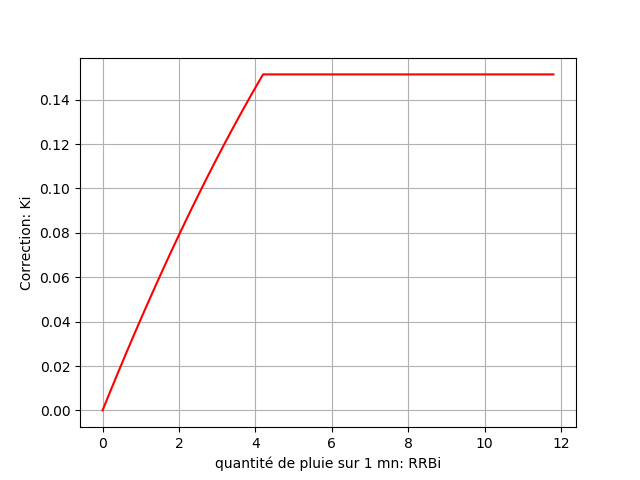
\includegraphics[scale=0.5]{./images/graph_formule_forte_pluie_K.png}
    \caption{Courbe de correction Ki en fonction de la quantit� de pluie par minute (pour un pluviom�tre pr�cis-m�canique 3070)}
\label{fig-formule}
\end{figure}
\end{center}

Et la Correction a appliquer a chaque minute $C_i$:
$$
C_i = K_i \times RRB_i
$$

Calcul de $RRC_i$: cumul des corrections � la minute $i$:

$$
RRC_i = RRB_i+INC_i
$$

$INC_i$ est la correction � appliquer au cumul des pr�cipitations \`a l'intant $i$ par pas de 0.1 mm. 
Si la correction $C_i$ n'atteint pas 0.1 mm, on garde le reste $RES_i$ en m�moire pour la minute suivante.
$RES_i$ est r�initialis� au bout de 2 minutes sans pluie.

$$
INC_i = \dfrac{\text{Partie Enti\`ere}  (10  \times ( Ci +RES_{i-1} ))}{10}
$$
$$
\text{et }  RES_i = \left\lbrace
\begin{array}{ll}
0 & \text{si } RRB_i = 0  \text{ et } RRB_{i-1} =0 \\
RES_{i-1}  + C_i  -INC_i & sinon \\
\end{array}\\
\right.
$$




%%%%%COMMENTAIRE%%%%
\itemstyle{Commentaire :}
Cette correction est utilis\'ee pour les pluvio pr�ci m�caniques du r�seau radome � la DSO.
\text{Valeurs des coefficients utilis�s pour le Pr\'ecis-m\'ecanique:}
$$
\begin{tabular}{lll}
A = -5.68 & B = 2.56 & C=0
\end{tabular}
$$



%%%%%AUTEUR%%%%

%%%%%AUTEUR%%%%
\itemstyle{Auteur~:}
CNRM/GMEI/TRAMM

%%%%%REFERENCE%%%%
\itemstyle{R\'ef\'erences~:}\\
Algorithme de traitement des donn\'ees du pr\'eci-M\'ecanique
Version 1.1 du 28/01/2013 DSO



\chapter{Micro-Physique}
%
%% MICRO-PHYSIQUE %%
%
\section{Eau liquide \`a partir des mesures d'un King Probe}

\itemstyle{ Op\'erateur~: } \operfmt{lwckp}
\index{lwckp}

%%%%%OBJET%%%%%
\itemstyle{ Objet~: }
Calcul du contenu en eau liquide \`a  de l'air
partir de la mesure de puissance fournie \`a 
l'\'el\'ement sensible (fil chaud) d'un King Probe.


%%%%%ARGUMENTS%%%%%
\bigskip
%%%%%ENTREES%%%%
\begin{tabarg}
\multicolumn{3}{l}{\titretab{ Entr\'ees}}\\
\hline
$P_w$ & Vecteur, \texttt{float} & Puissance fournie au fil chaud ($W$)\\
$T_s$ & Vecteur, \texttt{float} & Temp\'erature statique de l'air ($K$ ou $^\circ C$) \\
$P_s$ & Vecteur, \texttt{float} & Pression statique de l'air ($hPa$) \\
$V_p$ & Vecteur, \texttt{float} & Vitesse propre ($m/s$)\\
$l$ & Coeff., \texttt{float} & Longueur du fil chaud ($mm$)\\
$d$ & Coeff., \texttt{float} & Diam\`etre du fil chaud ($mm$)\\
$T_w$ & Coeff., \texttt{float} &  Temp\'erature du fil chaud en air clair ($K$)\\
$T_{wh}$ & Coeff., \texttt{float} & Temp\'erature du fil chaud en nuage ($K$)\\
$A$ & Coeff., \texttt{float} & Constante empirique pour le calcul de la dissipation en air sec\\
$\chi$ & Coeff., \texttt{float} & idem
\end{tabarg}

\medskip
%%%%%SORTIES%%%%
\begin{tabarg}
\multicolumn{3}{l}{\titretab{ Sorties}}\\
\hline
$LWC$ & Vecteur, \texttt{float} & Contenu en eau liquide ($gram/m^3$)\\
\end{tabarg}


%%%%%FORMULE%%%%
\itemstyle{ Formule }

% calcul du rapport de melange en eau liquide
% a partir de la mesure du King-Probe. 
\[
LWC = \frac{ P_w - A(T_w-T_s).(\rho.V_p)^\chi}
              { l.d.V_p.[ L+c.(T_{wh} - T_s) ] }
\]
avec $L = 2.264.10^6 J.kg^{-1}$ (chaleur latente de l'eau \`a $100^\circ C$) et
$c = 4218 J.kg^{-1}$ (chaleur sp\'ecifique de l'eau)

Le calcul n'est fait que si $V_p > 50.0 m/s$ et
$P_w > 3.0 Watt $


%%%%%AUTEUR%%%%%
\itemstyle{ Auteur~:}
CNRM/GMEI/TRAMM

%%%%%REFERENCES%%%%%
\itemstyle{ R\'ef\'erences~:}
P.M.S.'s Operating and Servicing Manual \cite{King}

\newpage
%% MICRO-PHYSIQUE %%
%
\section{Eau liquide \`a partir des mesures d'un lwc300}

\itemstyle{ Op\'erateur~: } \operfmt{lwc\_lwc300}
\index{lwc\_lwc300}

%%%%%OBJET%%%%%
\itemstyle{ Objet~: }
Calcul du contenu en eau liquide \`a  de l'air
partir de la mesure de puissance fournie \`a 
l'\'el\'ement sensible (fil chaud) d'un lwc300.


%%%%%ARGUMENTS%%%%%
\bigskip
%%%%%ENTREES%%%%
\begin{tabarg}
\multicolumn{3}{l}{\titretab{ Entr\'ees}}\\
\hline
$P_w$ & Vecteur, \texttt{float} & Puissance fournie au fil chaud ($W$)\\
$T_s$ & Vecteur, \texttt{float} & Temp\'erature statique de l'air ($K$ ou $^\circ C$) \\
$P_s$ & Vecteur, \texttt{float} & Pression statique de l'air ($hPa$) \\
$V_p$ & Vecteur, \texttt{float} & Vitesse propre ($m/s$)\\
$l$ & Coeff., \texttt{float} & Longueur du fil chaud ($mm$)\\
$d$ & Coeff., \texttt{float} & Diam\`etre du fil chaud ($mm$)\\
$T_w$ & Coeff., \texttt{float} &  Temp\'erature du fil chaud sp\'ecifi\'ee dans PADS ($K$ ou $^\circ C$)\\
\end{tabarg}

\medskip
%%%%%SORTIES%%%%
\begin{tabarg}
\multicolumn{3}{l}{\titretab{ Sorties}}\\
\hline
$LWC$ & Vecteur, \texttt{float} & Contenu en eau liquide ($gram/m^3$)\\
\end{tabarg}


%%%%%FORMULE%%%%
\itemstyle{ Formule }

% calcul du rapport de melange en eau liquide
% a partir de la mesure du King-Probe. 

Voir Hotwire LWC Module 3.5.0 Manual (Droplet Measurement Technologies)

Le calcul n'est fait que si $V_p > 50.0 m/s$ et
$P_w > 3.0 Watt $


%%%%%AUTEUR%%%%%
\itemstyle{ Auteur~:}
CNRM/GMEI/TRAMM

%%%%%REFERENCES%%%%%
\itemstyle{ R\'ef\'erences~:}
Hotwire LWC Module 3.5.0 Manual (Droplet Measurement Technologies)

\newpage
%%%%%
%
%% Dans ce fichier, les �ventuels accents sont cod�s
%% en ISO-8859-15 (aka latin9)
%% La ligne suivante donne trois exemples 
%% e accent aigu : �, e accent grave : �, e-dans-l'o : �
\section{Eau liquide \`a partir des mesures Robust}

\itemstyle{Op\'erateur~:} \operfmt{Calc\_lwc\_robust}
\index{Calc\_lwc\_robust}

%%%%%OBJET%%%%
\itemstyle{Objet~:}
Calcul du contenu en eau liquide � partir des donn\'ees 
de mesure de la sonde Robust.

%%%%%ARGUMENTS%%%%
\bigskip
%% Dans ce fichier, les �ventuels accents sont cod�s
%% en ISO-8859-15 (aka latin9)
%% La ligne suivante donne trois exemples 
%% e accent aigu : �, e accent grave : �, e-dans-l'o : �
%%%%%ENTREES%%%%
\begin{tabarg}
\multicolumn{3}{l}{\titretab {Entr\'ees}}\\
\hline
$P_s$ & Vecteur, \texttt{float} &  Pression statique de l'air ($hPa$)\\
$T_s$ & Vecteur, \texttt{float} & Temp�rature statique de l'air ($K$ ou $^\circ C$)\\
$V_p$ & Vecteur, \texttt{float} & Vitesse propre ($m/s$)\\
$P_w$ & Vecteur, \texttt{float} & Puissance fournie \`a la sonde ($W$)\\
$T_w$ & Vecteur, \texttt{float} & Temp\'erature de la sonde ($K$ ou $^\circ C$)\\
$K_1$ & Coeff., \texttt{float} & Coefficient de calcul de la puissance s\`eche Robust\\
$K_2$ & Coeff., \texttt{float} & Coefficient de calcul de la puissance s\`eche Robust\\
\end{tabarg}

\medskip
%%%%%SORTIES%%%%
\begin{tabarg}
\multicolumn{3}{l}{\titretab {Sorties}}\\
\hline
$LWC$ & Vecteur, \texttt{float} & Contenu en eau liquide ($g/m^3$)\\
\end{tabarg}


%%%%%FORMULE%%%%
\itemstyle{Formule}

% calcul du rapport de melange en eau liquide
% a partir de la mesure Robust. 

Voir SEA Operating Manual


%%%%%AUTEUR%%%%
\itemstyle{Auteur~:}
SAFIRE/ITD/TAD

%%%%%REFERENCE%%%%
\itemstyle{R\'ef\'erences~:}
SEA - Operating manual Model WCM-3000

\newpage
%%%%%%%%
%
\section{Rapport de m\'elange en eau liquide \`a partir
du "barreau" Sextant}

\itemstyle{Op\'erateur~:} {\sf lwcsex}
\index{lwcsex}

%%%%%OBJET%%%%
\itemstyle{Objet~:}
Calcul du rapport de m\'elange en eau liquide \`a partir
des mesures du "barreau" Sextant.

%%%%%ARGUMENTS%%%%
\bigskip
%%%%%ENTREES%%%%
\begin{tabarg}
\multicolumn{3}{l}{\titretab {Entr\'ees}}\\
\hline
$P_b$ & Vecteur, {\tt float} & Mesure puissance du barreau  ($V$)\\
$R_b$ & Vecteur, {\tt float} & Mesure temp\'erature du barreau ($V$)\\
$T_t$ & Vecteur, {\tt float} & Temp\'erature totale (impact) ($K$ ou
$^\circ C$)\\
$T_s$ & Vecteur, {\tt float} & Temp\'erature de l'air ($K$ ou
$^\circ C$)\\
$P_s$ & Vecteur, {\tt float} & Pression statique ($hPa$)\\
$V_p$ & Vecteur, {\tt float} & Vitesse propre ($m/s$)\\
\end{tabarg}

\medskip
%%%%%SORTIES%%%%
\begin{tabarg}
\multicolumn{3}{l}{\titretab {Sorties}}\\
\hline
$LWC$ & Vecteur, {\tt float} & Rapport de m\'elange en eau 
liquide ($g/m^3$)\\
\end{tabarg}


%%%%%FORMULE%%%%
\itemstyle{Formule}

%%% calcul LWC barreau Sextant
%%%
\begin{align*}
T_w &= \frac{1}
               {C_t[0]}.\left( 
          \frac{R_b}
               {C_t[1]} - 1 \right)	\\
P_w &= C_{pw}[0] .P_b . \frac{C_{pw}[1]}{R_b} \\  
P_{sec} &= C_p[0]. ( T_w - T_t).\left[
          \frac{P_s.V_p. (T_s +120)}
               {T_s^{5/2} }
          \right]^C_p[1] \\
LWC &= 1000 \times 
         \frac{ P_w - P_{sec} }
              {C_l[0].V_p.
               \left[ C_l[1] + C_l[2].\left(T_w - T_s \right)
               \right] } \\  
\end{align*}


%%%%%AUTEUR%%%%
\itemstyle{Auteur~:}
CNRM/GMEI/TRAMM

%%%%%REFERENCE%%%%
\itemstyle{R\'ef\'erences~:}
Obtenu aupr\`es de Sextant.

%%%\newpage
%%%%%
%
\section{FSSP: Activit� � partir l'enregistrement brut}

\itemstyle{Op\'erateur~:} \operfmt{fssp\_activ}
\index{fssp\_activ}

%%%%%OBJET%%%%
\itemstyle{Objet~:}
Calcul de l'activit� d'un FSSP exprim�e en proportion (gamme $[0, 1]$)
� partir de l'enregistrement brut de la voie "activit�".

L'enregistrement brut est bas� sur le comptage des pulsations
d'horloge dans les p�riodes pendant lesquelles la sonde
travaille (d�tection de gouttes, dimensionnement ou rejet).

Dans la sonde, le nombre de pulsations est divis�
par $2^x$, donc le coefficient est �gal �
$2^x$ / (fr�quence de l'horloge).


%%%%%ARGUMENTS%%%%
\bigskip
%%%%%ENTREES%%%%
\begin{tabarg}
\multicolumn{3}{l}{\titretab {Entr\'ees}}\\
\hline
$A_c$ & Vecteur, \texttt{float} & Activit\'e brute 
(\textit{comptes par p\'eriode d'\'echantillonnage})\\
$C_A$ & Coeff., \texttt{float} & Coefficient diviseur (1/ nombre de comptage max par seconde) \\
$f_e$ & Coeff., \texttt{float} & Fr\'equence d'\'echantillonnage ($Hz$)\\
\end{tabarg}

\medskip
%%%%%SORTIES%%%%
\begin{tabarg}
\multicolumn{3}{l}{\titretab {Sorties}}\\
\hline
$A_m$ & Vecteur, \texttt{float} & Activit\'e (proportion : $s$/$s$)\\
\end{tabarg}


%%%%%FORMULE%%%%
\itemstyle{Formule}

%%fssp_activ
\[
A_m = C_A.f_e.A_c
\]


%%%%%COMMENTAIRE%%%%
\itemstyle{Commentaire~:}
La valeur de $C_A$ pour le FSSP du CAM/SAFIRE est de 8.02e-6.

Pour d'autres FSSP, on trouve plut�t 1.00e-3.

%%%%%AUTEUR%%%%
\itemstyle{Auteur~:}
CNRM/GMEI/TRAMM

%%%%%REFERENCE%%%%
\itemstyle{R\'ef\'erences~:}
Brenguier-89 \cite{Brenguier-89}

\newpage
%%%%%
%
%% Dans ce fichier, les �ventuels accents sont cod�s
%% en ISO-8859-15 (aka latin9)
%% La ligne suivante donne trois exemples 
%% e accent aigu : �, e accent grave : �, e-dans-l'o : �
\section{FSSP: Calcul de l'activit� � partir des comptages}

\itemstyle{Op\'erateur~:} \operfmt{fssp\_activ\_calc}
\index{fssp\_activ\_calc}

%%%%%OBJET%%%%
\itemstyle{Objet~:}
Calcul de la fraction d'activit� d'une sonde de type FSSP, � partir des comptages
dans la DOF ("\texttt{strobe}") et hors de la DOF ("\texttt{fastreset}").


%%%%%ARGUMENTS%%%%
\bigskip
%% Dans ce fichier, les �ventuels accents sont cod�s
%% en ISO-8859-15 (aka latin9)
%% La ligne suivante donne trois exemples 
%% e accent aigu : �, e accent grave : �, e-dans-l'o : �
%%%%%ENTREES%%%%
\begin{tabarg}
\multicolumn{3}{l}{\titretab {Entr\'ees}}\\
\hline
$Strobe$ & Vecteur, \texttt{float} & Nombre de particules dans la DOF 
(\textit{comptes par p�riode d'�chantillonnage})\\
$Fast\_Reset$ & Vecteur, \texttt{float} & nombre de particules hors de la DOF
(\textit{comptes par p�riode d'�chantillonnage})\\
TAS & Vecteur, \texttt{float} & Vitesse propre (m/s)\\
$\tau{}_1$ & Coeff., \texttt{float} & d�lai long (second)\\
$\tau{}_2$ & Coeff., \texttt{float} & d�lai court (second)\\
\end{tabarg}

\medskip
%%%%%SORTIES%%%%
\begin{tabarg}
\multicolumn{3}{l}{\titretab {Sorties}}\\
\hline
$A_c$ & Vecteur, \texttt{float} & Activit� (proportion : $s$/$s$)\\
\end{tabarg}


%%%%%FORMULE%%%%
\itemstyle{Formule}

%% Formule de l'operateur : fssp_activ_calc
%% Dans ce fichier, les �ventuels accents sont cod�s
%% en ISO-8859-15 (aka latin9)
%% La ligne suivante donne trois exemples 
%% e accent aigu : �, e accent grave : �, e-dans-l'o : �
\[
\tau_T =  \frac{\Phi_{\text{Beam}} }{ \text{TAS} }
\]
\[
A_c = Strobe.(\tau_1 + \tau_T) + Fast\_Reset . (\tau_2 +\tau_T)
\]



%%%%%COMMENTAIRE%%%%
\itemstyle{Commentaire~:}
La formule de la note 24 du NCAR ne tient pas compte du temps
de transit moyen des gouttes dans le faisceau ($\tau_T$). Les
d�lais longs et courts ($\tau_1$ et $\tau_2$) sont des d�lais 
de traitement �lectronique, il est  donc logique de leur rajouter
le temps de transit moyen.

%%%%%AUTEUR%%%%
\itemstyle{Auteur~:}
CNRM/GMEI/TRAMM

%%%%%REFERENCE%%%%
\itemstyle{R\'ef\'erences~:}
Darrel Baumgardner, Bulletin NCAR/RAF n�24,
\textit{Airborne Measurements for Cloud Microphysics}.
\cite{RAF-24}

\newpage
%% THERMODYNAMIQUE %%
%
\section{FSSP : Temps de transit moyen}

\itemstyle{ Op\'erateur~: } {\sf fssp\_Tbar}
\index{fssp\_Tbar}

%%%%%OBJET%%%%%
\itemstyle{ Objet~: }
Calcul du temps de transit moyen d'une particule
dans le faisceau d'un FSSP. 

%%%%%ARGUMENTS%%%%%
\bigskip
%%%%%ENTREES%%%%
\begin{tabarg}
\multicolumn{3}{l}{\titretab{ Entr\'ees}}\\
\hline
$Strobe$ & Vecteur, {\tt float} & Nombre de particules dans la D.O.F (Depth Of Field) (\textit{comptes par p\'eriode d'\'echantillonnage})\\
$Reset$ & Vecteur, {\tt float} & Nombre de particules totales compt\'ees (\textit{comptes par p\'eriode d'\'echantillonnage})\\
$A_m $ & Vecteur, {\tt float} & Activit\'e de l'appareil \\
$f_e$ & Coeff., {\tt float} & Fr\'equence d'\'echantillonnage des donn\'ees ($Hz$) \\
$\tau_1$ & Coeff., {\tt float} & D\'elai \'electronique court ($s$)\\
$\tau_2$ & Coeff., {\tt float} & D\'elai \'electronique long ($s$)\\
$Crt_0$ & Coeff., {\tt float} & Taux de comptage minimal au dessus duquel on 
peut calculer le temps de transit ($s^{-1}$)\\
\end{tabarg}

\medskip
%%%%%SORTIES%%%%
\begin{tabarg}
\multicolumn{3}{l}{\titretab{ Sorties}}\\
\hline
$\overline{T}$ & Vecteur, {\tt float} & Temps de transit moyen d'une particule ($s$)\\
\end{tabarg}


%%%%%FORMULE%%%%
\itemstyle{ Formule }

%%%% Temps de transit moyen d'une particule
Si $Reset\times f_e \le Crt_0$ alors $\overline{T} = 0$ sinon~:
\begin{eqnarray*}
DOF & = & \frac{Strobe}{Reset} \\
\overline{T} & = & \frac{A_m}{f_e.Reset} - (1 - DOF).\tau_1 - DOF. \tau_2
\end{eqnarray*}


%%%%%AUTEUR%%%%%
\itemstyle{ Auteur~:}
CNRM/GMEI/TRAMM

%%%%%REFERENCES%%%%%
\itemstyle{ R\'ef\'erences~:}
Brenguier-89 \cite{Brenguier-89}.

\newpage
%%%%%
%
\section{FSSP: Temps de transit d\'eduit du spectre de gouttelettes
mesur\'e}

\itemstyle{Op\'erateur~:} {\sf fssp\_tauspec}
\index{fssp\_tauspec}

%%%%%OBJET%%%%
\itemstyle{Objet~:}
Calcul du temps transit d'une gouttelette \`a partir
du spectre mesur\'e par un FSSP.  

%%%%%ARGUMENTS%%%%
\bigskip
%%%%%ENTREES%%%%
\begin{tabarg}
\multicolumn{3}{l}{\titretab {Entr\'ees}}\\
\hline
$C_1$ & Vecteur, {\tt float} & Comptage dans la classe 1 
(\textit{comptes par p\'eriode d'\'echantillonnage}) \\
$C_2$ & Vecteur, {\tt float} & Comptage dans la classe 2 (\textit{idem})\\
$C_3$ & Vecteur, {\tt float} & Comptage dans la classe 3 (\textit{idem})\\
$C_4$ & Vecteur, {\tt float} & Comptage dans la classe 4 (\textit{idem})\\
$C_5$ & Vecteur, {\tt float} & Comptage dans la classe 5 (\textit{idem})\\
$C_6$ & Vecteur, {\tt float} & Comptage dans la classe 6 (\textit{idem})\\
$C_7$ & Vecteur, {\tt float} & Comptage dans la classe 7 (\textit{idem})\\
$C_8$ & Vecteur, {\tt float} & Comptage dans la classe 8 (\textit{idem})\\
$C_9$ & Vecteur, {\tt float} & Comptage dans la classe 9 (\textit{idem})\\
$C_{10}$ & Vecteur, {\tt float} & Comptage dans la classe 10 (\textit{idem})\\
$C_{11}$ & Vecteur, {\tt float} & Comptage dans la classe 11 (\textit{idem})\\
$C_{12}$ & Vecteur, {\tt float} & Comptage dans la classe 12 (\textit{idem})\\
$C_{13}$ & Vecteur, {\tt float} & Comptage dans la classe 13 (\textit{idem})\\
$C_{14}$ & Vecteur, {\tt float} & Comptage dans la classe 14 (\textit{idem})\\
$C_{15}$ & Vecteur, {\tt float} & Comptage dans la classe 15 (\textit{idem})\\
$V_p$ & Vecteur, {\tt float} & Vitesse propre ($m/s$)\\
$\phi_b$ & Coeff., {\tt float} & Diam\`etre du faisceau Laser ($m$) \\ 
$\tau_0$ & Coeff., {\tt float} & Temps de r\'eponse des amplificateurs ($s$)\\
$V_0$ & Coeff., {\tt float} & Seuil de d\'etection  ($mV$)\\
$V $ & Coeff., {\tt float[15]} & Seuil de d\'etection par classes ($mV$)\\
\end{tabarg}

\medskip
%%%%%SORTIES%%%%
\begin{tabarg}
\multicolumn{3}{l}{\titretab {Sorties}}\\
\hline
$\tau_{spec}$ & Vecteur, {\tt float} & Temps de transit ($s$)\\
\end{tabarg}


%%%%%FORMULE%%%%
\itemstyle{Formule}

%%fssp_tauspec
\begin{eqnarray*}
C_{{\tau}_k} & = & \tau_0 . \ln \left( \frac{V_k - V_0}{V_0} \right) \\
\tau_{spec} & = & \frac{\pi. \phi_b}{4.V_p} + 
                  \frac{\displaystyle\sum_{k=1}^{15} C_{{\tau}_k}.C_k}
                   {\displaystyle\sum_{k=1}^{15} C_k} \\
\end{eqnarray*}


%%%%%AUTEUR%%%%
\itemstyle{Auteur~:}
CNRM/GMEI/TRAMM

%%%%%REFERENCE%%%%
\itemstyle{R\'ef\'erences~:}
Brenguier-89 \cite{Brenguier-89}

\newpage
%%%%%
%
\section{FSSP : Correction des co\"{\i}ncidences par le
taux de comptage et l'activit\'e }

\itemstyle{Op\'erateur~:} {\sf fssp\_ncor\_acrs}
\index{fssp\_ncor\_acrs}

%%%%%OBJET%%%%
\itemstyle{Objet~:}
Calcul du nombre de gouttelettes total en tenant
compte des co\"{\i}ncidences. La m\'ethode employ\'ee
utilise \`a la fois le taux de comptage et l'activit\'e. 

%%%%%ARGUMENTS%%%%
\bigskip
%%%%%ENTREES%%%%
\begin{tabarg}
\multicolumn{3}{l}{\titretab {Entr\'ees}}\\
\hline
$Strobe$ & Vecteur, {\tt float} & Nombre de gouttelettes dans la D.O.F 
(Depth Of Field) (\textit{comptes par p\'eriode d'\'echantillonnage}) \\
$Reset$ & Vecteur, {\tt float} & Nombre total de gouttelettes compt\'ees 
(\textit{comptes par p\'eriode d'\'echantillonnage}) \\
$A_m$ & Vecteur, {\tt float} & Activit\'e de l'appareil \\
$\overline{T}$ & Vecteur, {\tt float} & Temps de transit moyen ($s$)\\
$f_e$ & Coeff., {\tt float} & Fr\'equence d'\'echantillonnage ($Hz$)\\
$\tau_1$ & Coeff., {\tt float} & D\'elai \'electronique court ($s$)\\
$\tau_2$ & Coeff., {\tt float} & D\'elai \'electronique long ($s$)\\
$\tau_r$ & Coeff., {\tt float} & D\'elai \'electronique du reset ($s$)\\
$Crt_0$ & Coeff., {\tt float} & Taux de comptage minimal au dessus duquel on
peut calculer le temps de transit ($s^{-1}$) \\
\end{tabarg}

\medskip
%%%%%SORTIES%%%%
\begin{tabarg}
\multicolumn{3}{l}{\titretab {Sorties}}\\
\hline
$N_{acrs}$ & Vecteur, {\tt float} & Nombre total de gouttes corrig\'e des 
co\"{\i}ncidences (\textit{comptes par p\'eriode d'\'echantillonnage}) \\
$\tau_{acrs}$ & Vecteur, {\tt float} & Temps de transit calcul\'e en tenant
compte des co\"{\i}ncidences (s)\\
\end{tabarg}


%%%%%FORMULE%%%%
\itemstyle{Formule}

%%fssp_ncor_acrs
L'algorithme et les formules \'etant complexes
seul le principe de calcul est pr\'esent\'e ici.\\
Selon Brenguier-89, l'activit\'e
et le nombre de gouttes mesur\'ees par un FSSP
s'expriment comme 2 fonctions~: \\ 
$$
\left\{
\begin{array}{rcl}
A & = & f_a ( N_c, \tau, \tau_1, \tau_2, \tau_r ) \\
N & = & f_n ( N_c, \tau, \tau_1, \tau_2, \tau_r ) \\
\end{array}
\right.
$$
o\`u~:\\
$N $ : nombre total de gouttes compt\'ees \\
$A $ : Activit\'e \\
$N_c$ : nombre total de gouttes corrig\'e des
co\"{\i}ncidences \\
$\tau $ : temps de transit d'une particule \\
\\
Avec $A=A_m$ et $N=Reset$, le syst\`eme poss\`ede 2
inconnues, $\tau$ et $N_c$. Il est
r\'esolu par it\'erations successives. $N_{acrs}$
et $\tau_{acrs}$ sont les r\'esultats.\\ 
Si $Reset\times f_e \le Crt_0$ alors aucune correction
est calcul\'ee et $N_{acrs}=0$ et $\tau_{acrs}=0$.



%%%%%AUTEUR%%%%
\itemstyle{Auteur~:}
CNRM/GMEI/TRAMM

%%%%%REFERENCE%%%%
\itemstyle{R\'ef\'erences~:}
Brenguier-89 \cite{Brenguier-89}

\newpage
%%%%%
%
\section{FSSP: Correction des co\"{\i}ncidences avec d'une part le
taux de comptage et d'autre part l'activit\'e }

\itemstyle{Op\'erateur~:} {\sf fssp\_ncor\_specacr}
\index{fssp\_ncor\_specacr}

%%%%%OBJET%%%%
\itemstyle{Objet~:}
Calcul du nombre de gouttelettes total en tenant
compte des co\"{\i}ncidences. Deux m\'ethodes
sont employ\'ees. L'une utilise uniquement le taux
de comptage et l'autre uniquement l'activit\'e.

%%%%%ARGUMENTS%%%%
\bigskip
%%%%%ENTREES%%%%
\begin{tabarg}
\multicolumn{3}{l}{\titretab {Entr\'ees}}\\
\hline
$Strobe$ & Vecteur, {\tt float} & Nombre de gouttelettes dans la D.O.F
(Depth Of Field) (\textit{comptes par p\'eriode d'\'echantillonnage}) \\
$Reset$ & Vecteur, {\tt float} & Nombre total de gouttelettes compt\'ees
(\textit{comptes par p\'eriode d'\'echantillonnage}) \\
$A_m$ & Vecteur, {\tt float} & Activit\'e de l'appareil \\
$\tau_{spec}$ & Vecteur, {\tt float} & Temps de transit estim\'e \`a
partir du spectre de gouttelettes mesur\'e ($s$)\\
$f_e$ & Coeff., {\tt float} & Fr\'equence d'\'echantillonnage ($Hz$)\\
$\tau_1$ & Coeff., {\tt float} & D\'elai \'electronique court ($s$)\\
$\tau_2$ & Coeff., {\tt float} & D\'elai \'electronique long ($s$)\\
$\tau_r$ & Coeff., {\tt float} & D\'elai \'electronique pour le reset ($s$)\\
$Crt_0$ & Coeff., {\tt float} & Taux de comptage minimal au dessus
duquel on peut effectuer la correction ($s^{-1}$) \\

\end{tabarg}

\medskip
%%%%%SORTIES%%%%
\begin{tabarg}
\multicolumn{3}{l}{\titretab {Sorties}}\\
\hline
$N_{ac}$ & Vecteur, {\tt float} & Nombre total de gouttelettes
corrig\'e des co\"{\i}ncidences par l'activit\'e
(\textit{comptes par p\'eriode d'\'echantillonnage}) \\
$N_{rs}$ & Vecteur, {\tt float} & Nombre total de gouttelettes
corrig\'e des co\"{\i}ncidences par le taux de comptage
(\textit{comptes par p\'eriode d'\'echantillonnage}) \\
\end{tabarg}


%%%%%FORMULE%%%%
\itemstyle{Formule}

%%fssp_ncor_specacr
L'algorithme et les formules \'etant complexes
seul le principe de calcul est pr\'esent\'e ici.\\
Selon Brenguier-89 \cite{Brenguier-89}, l'activit\'e
et le nombre de gouttes mesur\'ees par un FSSP
s'expriment comme 2 fonctions~: \\ 
\begin{eqnarray}
A & = & f_a ( N_c, \tau, \tau_1, \tau_2, \tau_r )  \label{eqn:acti}\\
N & = & f_n ( N_c, \tau, \tau_1, \tau_2, \tau_r ) \label{eqn:crt}
\end{eqnarray}
o\`u~:\\
$N$ : nombre total de gouttes compt\'ees \\
$A $ : Activit\'e \\
$N_c$ : nombre total de gouttes corrig\'e des
co\"{\i}ncidences \\
$\tau $ : temps de transit d'une particule \\
\\
On pose $\tau = \tau_{spec}$, $A=A_m$, et $N=Reset$.
Ainsi, chaque \'equation ne
poss\`ede plus qu'une inconnue $N_c$. 
Elles sont r\'esolues s\'epar\'ement par it\'erations successives.   
(\ref{eqn:acti}) donne $N_{ac}$ et (\ref{eqn:crt}) 
donne $N_{rs}$.\\
Si $Reset\times f_e \le Crt_0$ alors aucune correction
est calcul\'ee et $N_{ac}=0$ et $N_{rs}=0$.


%%%%%AUTEUR%%%%
\itemstyle{Auteur~:}
CNRM/GMEI/TRAMM

%%%%%REFERENCE%%%%
\itemstyle{R\'ef\'erences~:}
Brenguier-89 \cite{Brenguier-89}

\newpage
%%%%%
%
\section{FSSP: Correction des co\"{\i}ncidences avec le
taux de comptage}

\itemstyle{Op\'erateur:} {\sf fssp\_ncor\_specrs}
\index{fssp\_ncor\_specrs}

%%%%%OBJET%%%%
\itemstyle{Objet:}
Calcul du nombre de goutelettes total en corrig\'e des co\"{\i}ncidences; m\'ethode
utilisant uniquement le taux de comptage.

%%%%%ARGUMENTS%%%%
\bigskip
%%%%%ENTREES%%%%
\begin{tabarg}
\multicolumn{3}{l}{\titretab {Entr\'ees}}\\
\hline
$Strobe$ & Vecteur, {\tt float} & Nombre de particules dans la D.O.F.
   (comptes par p\'eriode d'\'echantillonnage)\\
$Reset$& Vecteur, {\tt float} & Nombre total de particules compt\'ees 
    (comptes par p\'eriode d'\'echantillonnage)\\
$\tau_{spec}$ & Vecteur, {\tt float} & temps de transit estim\'e \`a
          partir du spectre de gouttes ($s$)\\
$f_e$ & Coeff., {\tt float} & Fr\'equence d'\'echantillonnage ($Hz$)\\
$\tau_1$ & Coeff., {\tt float} & D\'elai \'electronique court ($s$)\\
$\tau_2$ & Coeff., {\tt float} & D\'elai \'electronique long ($s$)\\
$\tau_r$ & Coeff., {\tt float} & D\'elai \'electronique pour le reset ($s$)\\
$Crt_0$ & Coeff., {\tt float} & Taux de comptage minimal au dessus
duquel on peut effectuer la correction ($count.second^{-1}$)\\
\end{tabarg}

\medskip
%%%%%SORTIES%%%%
\begin{tabarg}
\multicolumn{3}{l}{\titretab {Sorties}}\\
\hline
$N_{rs}$ & Vecteur, {\tt float} & Nombre total de gouttelettes
corrig\'e des co\"{\i}ncidences par le taux de comptage
(\textit{comptes par p\'eriode d'\'echantillonnage}) \\
\end{tabarg}


%%%%%FORMULE%%%%
\itemstyle{Formule}

%%fssp_ncor_specrs

L'algorithme et les formules \'etant complexes
seul le principe de calcul est pr\'esent\'e ici.\\
Selon Brenguier-89 \cite{Brenguier-89}, 
le nombre de gouttes mesur\'ees par un FSSP
s'exprime comme une fonction~: \\ 
\begin{eqnarray}
N & = & f_n ( N_c, \tau, \tau_1, \tau_2, \tau_r ) \label{eqn:crt2}
\end{eqnarray}
o\`u~:\\
$N$ : nombre total de gouttes compt\'ees \\
$N_c$ : nombre total de gouttes corrig\'e des
co\"{\i}ncidences \\
$\tau $ : temps de transit d'une particule \\
\\
On pose $\tau = \tau_{spec}$, et $N=Reset$.
Ainsi, cette \'equation ne
poss\`ede plus qu'une inconnue $N_c$. 
Elle est r\'esolue par it\'erations successives.   
(\ref{eqn:crt2}) donne $N_{rs}$.\\
Si $Reset\times f_e \le Crt_0$ alors aucune correction
est calcul\'ee et $N_{ac}=0$ et $N_{rs}=0$.


%%%%%AUTEUR%%%%
\itemstyle{Commentaire:}
Le calcul est identique \`a celui fait dans \textsf{fssp\_ncor\_specacr},
sans prendre en compte l'activit\'e. Le r\'esultat est de moindre
qualit\'e, on n'utilisera donc cette formule que dans les cas o\`u
l'activit\'e n'a pas \'et\'e mesur\'ee.

%%%%%AUTEUR%%%%
\itemstyle{Auteur:}
CNRM/GMEI/TRAMM

%%%%%REFERENCE%%%%
\itemstyle{R\'ef\'erences:}
Brenguier-89\cite{Brenguier-89}

\newpage
%%%%%
%
\section{FSSP : Correction des co\"{\i}ncidences par
la m\'ethode "locale" }

\itemstyle{Op\'erateur~:} {\sf fssp\_ncor\_loc}
\index{fssp\_ncor\_loc}

%%%%%OBJET%%%%
\itemstyle{Objet~:}
Calcul du nombre de gouttelettes total en tenant compte
des co\"{\i}ncidences. Le temps de transit calcul\'e 
est compar\'e au temps de transit mesur\'e ($\tau_{spec}$).


%%%%%ARGUMENTS%%%%
\bigskip
%%%%%ENTREES%%%%
\begin{tabarg}
\multicolumn{3}{l}{\titretab {Entr\'ees}}\\
\hline
$Strobe$ & Vecteur, {\tt float} & Nombre de gouttelettes dans la D.O.F
(Depth Of Field) (\textit{comptes par p\'eriode d'\'echantillonnage}) \\
$Reset$ & Vecteur, {\tt float} & Nombre total de gouttelettes
compt\'ees (\textit{comptes par p\'eriode d'\'echantillonnage}) \\
$A_m$ & Vecteur, {\tt float} & Activit\'e de l'appareil \\
$\overline{T}$ & Vecteur, {\tt float} & Temps de transit moyen ($s$)\\
$\tau_{spec}$ & Vecteur, {\tt float} & Temps de transit estim\'e \`a 
partir du spectre de gouttelettes mesur\'e \\
$f_e$ & Coeff., {\tt float} & Fr\'equence d'\'echantillonnage ($Hz$)\\
$\tau_1$ & Coeff., {\tt float} & D\'elai electronique court ($s$)\\
$\tau_2$ & Coeff., {\tt float} & D\'elai electronique long ($s$)\\
$\tau_r$ & Coeff., {\tt float} & D\'elai electronique pour le reset ($s$)\\
$Crt_0$ & Coeff., {\tt float} & Taux de comptage minimal au dessus
duquel on peut effectuer la correction ($s^{-1}$) \\
\end{tabarg}

\medskip
%%%%%SORTIES%%%%
\begin{tabarg}
\multicolumn{3}{l}{\titretab {Sorties}}\\
\hline
$N_{loc}$ & Vecteur, {\tt float} & Nombre total de gouttelettes
corrig\'e des co\"{\i}ncidences (\textit{comptes par p\'eriode
d'\'echantillonnage}) \\
$H_c$ & Vecteur, {\tt float} & Homogene\"{\i}t\'e calcul\'ee\\
\end{tabarg}


%%%%%FORMULE%%%%
\itemstyle{Formule}

%%fssp_ncor_specacr
L'algorithme et les formules \'etant complexes
seul le principe de calcul est pr\'esent\'e ici.\\
Selon Brenguier-89 \cite{Brenguier-89}, le
temps de transit moyen d'une gouttelettes   
s'exprime comme une fonction~: \\ 
\begin{equation}
\overline{T}_c = f_{\overline{T}} ( N_c, \tau, \tau_1, \tau_2, \tau_r )
\label{eqn:tbar}  
\end{equation}
o\`u~:\\
$\overline{T_c} $ : Temps de transit moyen \\
$N_c$ : nombre de gouttes corrig\'e des
co\"{\i}ncidences \\
$\tau $ : temps de transit d'une particule \\
\\
On pose $\tau = \tau_{spec}$, $\overline{T}_c = \overline{T}$.
L'\'equation (\ref{eqn:tbar}) ne poss\`ede plus qu'une inconnue $N_c$. 
Elle est r\'esolue par it\'erations successives et donne  
$N_{loc}$.  $H_c$ est calcul\'e par
$H_c = A_m/A$ o\`u 
$A = f_A(N_{loc}, \tau_{spec}, \tau_1, \tau_2, \tau_r )$.\\ 
Si $Reset\times f_e \le Crt_0$ alors aucune correction
est calcul\'ee et $N_{loc}=0$ et $H_c=0$.


%%%%%AUTEUR%%%%
\itemstyle{Auteur~:}
CNRM/GMEI/TRAMM

%%%%%REFERENCE%%%%
\itemstyle{R\'ef\'erences~:}
Brenguier-89 \cite{Brenguier-89}.

\newpage
%%%%%
%
\section{FSSP: Concentration de gouttelettes totale }

\itemstyle{Op\'erateur~:} {\sf fssp\_tconc}
\index{fssp\_tconc}

%%%%%OBJET%%%%
\itemstyle{Objet~:}
Calcul de concentration totale des gouttelettes 
mesur\'ees par un FSSP.

%%%%%ARGUMENTS%%%%
\bigskip
%%%%%ENTREES%%%%
\begin{tabarg}
\multicolumn{3}{l}{\titretab {Entr\'ees}}\\
\hline
$Strobe$ & Vecteur, {\tt float} & Nombre de gouttelettes dans la D.O.F
(Depth Of Field) (\textit{comptes par p\'eriode d'\'echantillonnage})\\
$V_p$ & Vecteur, {\tt float} &  Vitesse propre ($m/s$)\\
$f_e$ & Coeff., {\tt float} &  Fr\'equence d'\'echantillonnage ($Hz$)\\
$S_{dof}$ & Coeff., {\tt float} & Section de la D.O.F ($mm^2$)\\
\end{tabarg}

\medskip
%%%%%SORTIES%%%%
\begin{tabarg}
\multicolumn{3}{l}{\titretab {Sorties}}\\
\hline
$Conc$ & Vecteur, {\tt float} & Concentration totale des gouttelettes ($cm{-3}$)\\
\end{tabarg}


%%%%%FORMULE%%%%
\itemstyle{Formule}

% calcul de la concentration totale de gouttes
% pour le FSSP standard
$$
Conc = \frac{Strobe.f_e}{S_{dof}.V_p}  
$$


%%%%%AUTEUR%%%%
\itemstyle{Auteur~:}
CNRM/GMEI/TRAMM

%%%%%REFERENCE%%%%
\itemstyle{R\'ef\'erences~:}
Bulletin NCAR-RAF Nr 24 \cite{RAF-24}


\newpage
%%%%%
%
\section{FSSP: Concentration de gouttelettes dans une classe}

\itemstyle{Op\'erateur~:} \operfmt{fssp\_conc\_part}
\index{fssp\_conc\_part}

%%%%%OBJET%%%%
\itemstyle{Objet~:}
Calcul de la concentration de gouttelettes dans une classe 
de mesure d'un FSSP.

%%%%%ARGUMENTS%%%%
\bigskip
%%%%%ENTREES%%%%
\begin{tabarg}
\multicolumn{3}{l}{\titretab {Entr\'ees}}\\
\hline
$C_k$ & Vecteur, \texttt{float} & Nombre de gouttelettes dans la classe $k$ 
(\textit{comptes par p\'eriode d'\'echantillonnage})\\
$C_T$ & Vecteur, \texttt{float} & Nombre total de gouttelettes dans toutes les classes
(\textit{comptes par p\'eriode d'\'echantillonnage})\\
$Conc$ & Vecteur, \texttt{float} & Concentration totale de gouttelettes ($cm^{-3}$)\\
\end{tabarg}

\medskip
%%%%%SORTIES%%%%
\begin{tabarg}
\multicolumn{3}{l}{\titretab {Sorties}}\\
\hline
$Conc_k$ & Vecteur, \texttt{float} & Concentration de gouttelettes 
                                  dans la classe $k$ ($cm^{-3}$)\\
\end{tabarg}


%%%%%FORMULE%%%%
\itemstyle{Formule}

%%fssp_conc_part
\[
Conc_k = \frac{C_k . Conc}{C_T} 
\]


%%%%%AUTEUR%%%%
\itemstyle{Auteur~:}
CNRM/GMEI/TRAMM

%%%%%REFERENCE%%%%
\itemstyle{R\'ef\'erences~:}
Bulletin NCAR-RAF Nr 24 \cite{RAF-24}

\newpage
%%%%%
%
\section{Tableau des concentrations � partir des comptages et de la concentration totale}

\itemstyle{Op\'erateur~:} \operfmt{fssp\_conc\_tab}
\index{fssp\_conc\_tab}

%%%%%OBJET%%%%
\itemstyle{Objet~:}
Calcul du tableau des concentrations � partir
du tableau des comptages et de la concentration totale.

%%%%%ARGUMENTS%%%%
\bigskip
%%%%%ENTREES%%%%
\begin{tabarg}
\multicolumn{3}{l}{\titretab {Entr\'ees}}\\
\hline
$C$ & Vecteur, \texttt{float[$d$]} & Tableau des comptages (\textit{comptes par p\'eriode d'\'echantillonnage})\\
$d$ & Coeff., \texttt{Int\_32} & Taille de la dimension (hors-temps) de $C$\\
$Conc_{T}$ & Vecteur, \texttt{float} & Concentration totale de gouttelettes (cm$^{-3}$)\\
\end{tabarg}

\medskip
%%%%%SORTIES%%%%
\begin{tabarg}
\multicolumn{3}{l}{\titretab {Sorties}}\\
\hline
$Conc$ & Vecteur, \texttt{float[$d$]} & Tableau des concentrations (m�me unit� que $Conc_{T}$)\\
\end{tabarg}


%%%%%FORMULE%%%%
\itemstyle{Formule}

%%fssp_conc_tab
\[
C_T = \sum_{k=1}^{d} C_k
\]
\[
Conc_k = \frac{C_k . Conc_T}{C_T} \qquad k=1,d
\]



%%%%%AUTEUR%%%%
\itemstyle{Auteur~:}
CNRM/GMEI/TRAMM

%%%%%REFERENCE%%%%
\itemstyle{R\'ef\'erences~:}
Bulletin NCAR-RAF Nr 24 \cite{RAF-24}

\newpage
%%%%%
%
\section{FSSP: Concentration de gouttelettes totale corrig\'ee }

\itemstyle{Op\'erateur~:} {\sf fssp\_tconc\_cor}
\index{fssp\_tconc\_cor}

%%%%%OBJET%%%%
\itemstyle{Objet~:}
Calcul de la concentration totale des gouttelettes \`a partir
d'un nombre total de gouttelettes corrig\'e. 

%%%%%ARGUMENTS%%%%
\bigskip
%%%%%ENTREES%%%%
\begin{tabarg}
\multicolumn{3}{l}{\titretab {Entr\'ees}}\\
\hline
$Strobe$ & Vecteur, {\tt float} & Nombre de gouttelettes dans la D.O.F
(Depth Of Field) (\textit{comptes par p\'eriode d'\'echantillonnage}) \\
$Reset$ & Vecteur, {\tt float} & Nombre total de gouttelettes  
compt\'ees (\textit{comptes par p\'eriode d'\'echantillonnage}) \\
$N_t$ & Vecteur, {\tt float} & Nombre total de gouttelettes corrig\'e 
(\textit{comptes par p\'eriode d'\'echantillonnage})\\
$V_p$ & Vecteur, {\tt float} & Vitesse propre ($m/s$)\\
$f_e$ & Coeff., {\tt float} & Fr\'equence d'\'echantillonnage ($Hz$)\\
$S_{dof}$ & Coeff., {\tt float} &  Section de la D.O.F ($mm^2$)\\
\end{tabarg}

\medskip
%%%%%SORTIES%%%%
\begin{tabarg}
\multicolumn{3}{l}{\titretab {Sorties}}\\
\hline
$Conc$ & Vecteur, {\tt float} & Concentration totale des gouttelettes
($cm^{-3}$) \\
\end{tabarg}


%%%%%FORMULE%%%%
\itemstyle{Formule}

%%fssp_tconc_cor
\begin{eqnarray*}
DOF & = & \frac{Strobe}{Reset} \\
Conc & =  & \frac{N_t.f_e.DOF}{S_{dof}.V_p} \\ 
\end{eqnarray*}


%%%%%AUTEUR%%%%
\itemstyle{Auteur~:}
CNRM/GMEI/TRAMM

%%%%%REFERENCE%%%%
\itemstyle{R\'ef\'erences~:}
Bulletin NCAR-RAF Nr 24 \cite{RAF-24}

\newpage
%%%%%
%
\section{FSSP: Rapport de m\'elange en eau liquide }

\itemstyle{Op\'erateur~:} {\sf fssp\_lwc}
\index{fssp\_lwc}

%%%%%OBJET%%%%
\itemstyle{Objet~:}
Calcul du rapport de m\'elange en eau liquide \`a
partir du nombre de gouttelettes compt\'ees dans chaque
classe d'un FSSP.

%%%%%ARGUMENTS%%%%
\bigskip
%%%%%ENTREES%%%%
\begin{tabarg}
\multicolumn{3}{l}{\titretab {Entr\'ees}}\\
\hline
$C_1$ & Vecteur, {\tt float} & Comptage dans la classe 1 
(\textit{comptes par p\'eriode d'\'echantillonnage})\\
$C_2$ & Vecteur, {\tt float} & Comptage dans la classe 2  (\textit{idem})\\
$C_3$ & Vecteur, {\tt float} & Comptage dans la classe 3  (\textit{idem})\\
$C_4$ & Vecteur, {\tt float} & Comptage dans la classe 4  (\textit{idem})\\
$C_5$ & Vecteur, {\tt float} & Comptage dans la classe 5  (\textit{idem})\\
$C_6$ & Vecteur, {\tt float} & Comptage dans la classe 6  (\textit{idem})\\
$C_7$ & Vecteur, {\tt float} & Comptage dans la classe 7  (\textit{idem})\\
$C_8$ & Vecteur, {\tt float} & Comptage dans la classe 8  (\textit{idem})\\
$C_9$ & Vecteur, {\tt float} & Comptage dans la classe 9  (\textit{idem})\\
$C_{10}$ & Vecteur, {\tt float} & Comptage dans la classe 10 (\textit{idem})\\
$C_{11}$ & Vecteur, {\tt float} & Comptage dans la classe 11 (\textit{idem})\\
$C_{12}$ & Vecteur, {\tt float} & Comptage dans la classe 12 (\textit{idem})\\
$C_{13}$ & Vecteur, {\tt float} & Comptage dans la classe 13 (\textit{idem})\\
$C_{14}$ & Vecteur, {\tt float} & Comptage dans la classe 14 (\textit{idem})\\
$C_{15}$ & Vecteur, {\tt float} & Comptage dans la classe 15 (\textit{idem})\\
$Conc$ & Vecteur, {\tt float} & Concentration totale de gouttelettes ($cm^{-3}$)\\
$\phi$ & Coeff., {\tt float[15]} & Diam\`etre moyen dans chaque classe ($\mu m$)\\
\end{tabarg}

\medskip
%%%%%SORTIES%%%%
\begin{tabarg}
\multicolumn{3}{l}{\titretab {Sorties}}\\
\hline
$LWC$ & Vecteur, {\tt float} &  Rapport de m\'elange en eau liquide ($g/m^3$)\\
\end{tabarg}


%%%%%FORMULE%%%%
\itemstyle{Formule}

%%fssp_lwc
\[
LWC = \rho_w .\frac{\pi}{6}. Conc .
\frac{\displaystyle\sum_{k=1}^{15} \phi^3_k.C_k}
     {\displaystyle\sum_{k=1}^{15} C_k}
\]
avec $\rho_w = 1000 kg/m^3$


%%%%%AUTEUR%%%%
\itemstyle{Auteur~:}
CNRM/GMEI/TRAMM

%%%%%REFERENCE%%%%
\itemstyle{R\'ef\'erences~:}
Bulletin NCAR-RAF Nr 24 \cite{RAF-24}

\newpage
%%%%%
%
\section{FSSP: Rapport de m\'elange en eau liquide, pour 
des classes lin\'eaires en diam\`etre}

\itemstyle{Op\'erateur~:} \operfmt{fssp\_lwc\_lin}
\index{fssp\_lwc\_lin}
\label{OP-fssp_lwc_lin}

%%%%%OBJET%%%%
\itemstyle{Objet~:}
Calcul du rapport de m\'elange en eau liquide \`a
partir de 15 comptages de gouttelettes dans les classes
d'un granulom�tre et de la concentration totale, dans le 
cas o� le diam\`etre moyen de chaque classe est une fonction
lin\'eaire de la classe.

%%%%%ARGUMENTS%%%%
\bigskip
%%%%%ENTREES%%%%
\begin{tabarg}
\multicolumn{3}{l}{\titretab {Entr\'ees}}\\
\hline
$C_1$ & Vecteur, \texttt{float} & Comptage dans la classe 1 
(\textit{comptes par p\'eriode d'\'echantillonnage})\\
$C_2$ & Vecteur, \texttt{float} & Comptage dans la classe 2 (\textit{idem})\\
\vdots & \vdots & \vdots \\
%$C_3$ & Vecteur, \texttt{float} & Comptage dans la classe 3 (\textit{idem})\\
%$C_4$ & Vecteur, \texttt{float} & Comptage dans la classe 4 (\textit{idem})\\
%$C_5$ & Vecteur, \texttt{float} & Comptage dans la classe 5 (\textit{idem})\\
%$C_6$ & Vecteur, \texttt{float} & Comptage dans la classe 6 (\textit{idem})\\
%$C_7$ & Vecteur, \texttt{float} & Comptage dans la classe 7 (\textit{idem})\\
%$C_8$ & Vecteur, \texttt{float} & Comptage dans la classe 8 (\textit{idem})\\
%$C_9$ & Vecteur, \texttt{float} & Comptage dans la classe 9 (\textit{idem})\\
%$C_{10}$ & Vecteur, \texttt{float} & Comptage dans la classe 10 (\textit{idem})\\
%$C_{11}$ & Vecteur, \texttt{float} & Comptage dans la classe 11 (\textit{idem})\\
%$C_{12}$ & Vecteur, \texttt{float} & Comptage dans la classe 12 (\textit{idem})\\
%$C_{13}$ & Vecteur, \texttt{float} & Comptage dans la classe 13 (\textit{idem})\\
%$C_{14}$ & Vecteur, \texttt{float} & Comptage dans la classe 14 (\textit{idem})\\
$C_{15}$ & Vecteur, \texttt{float} & Comptage dans la classe 15 (\textit{idem})\\
$Conc$ & Vecteur, \texttt{float} & Concentration totale de 
gouttelettes ($cm^{-3}$)\\
$a$ & Coeff., \texttt{float} & Coefficient de proportionnalit\'e pour le calcul du diam\`etre moyen de chaque classe ($\mu m$)\\
$b$ & Coeff., \texttt{float} & Coefficient constant pour le calcul du diam\`etre moyen de chaque classe($\mu m$)\\
\end{tabarg}

\medskip
%%%%%SORTIES%%%%
\begin{tabarg}
\multicolumn{3}{l}{\titretab {Sorties}}\\
\hline
$LWC$ & Vecteur, \texttt{float} & Rapport de m\'elange en eau liquide ($g/m^3$)\\
\end{tabarg}


%%%%%FORMULE%%%%
\itemstyle{Formule}

% calcul du rapport de m\'elange en eau liquide 
% a partir de la mesure du FSSP standard.
\begin{align*}
\phi_k &= a \cdot k + b  \\
LWC &=  \rho_w .\frac{\pi}{6}. Conc .
\frac{\displaystyle\sum_{k=1}^{15} \phi_k^3.C_k} 
     {\displaystyle\sum_{k=1}^{15} C_k}
\end{align*}
avec $\rho_w = 1000 kg/m^3$


%%%%% COMMENTAIRE %%%
\itemstyle{ Commentaire~: }
Si les comptages sont disponibles sous 
la forme d'un tableau, utiliser l'op�rateur 
\hyperref[OP-fssp_lwc_lin_tab]{\operfmt{fssp\_lwc\_lin\_tab}}.


%%%%%AUTEUR%%%%
\itemstyle{Auteur~:}
CNRM/GMEI/TRAMM

%%%%%REFERENCE%%%%
\itemstyle{R\'ef\'erences~:}
Bulletin NCAR-RAF Nr 24 \cite{RAF-24}.

\newpage
%%%%%
%
\section{FSSP: Rapport de m\'elange en eau liquide, pour 
des classes lin\'eaires en diam\`etre}

\itemstyle{Op\'erateur~:} \operfmt{fssp\_lwc\_lin\_tab}
\label{OP-fssp_lwc_lin_tab}
\index{fssp\_lwc\_lin\_tab}

%%%%%OBJET%%%%
\itemstyle{Objet~:}
Calcul du rapport de m\'elange en eau liquide (g/m3)
� partir d'un tableau de comptages issu d'un granulom�tre
et d'une concentration totale, pour le cas o�
le diam�tre moyen dans chaque classe est
une fonction lin�aire du num�ro de classe.

%%%%%ARGUMENTS%%%%
\bigskip
%%%%%ENTREES%%%%
\begin{tabarg}
\multicolumn{3}{l}{\titretab {Entr\'ees}}\\
\hline
$C$ & Vecteur, \texttt{float[15]} & Tableau des comptages ()\\
$Conc$ & Vecteur, \texttt{float} & Concentration totale de gouttelettes (cm$^{-3}$)\\
$a$ & Coeff., \texttt{float} & Terme de proportionnalit� du calcul du diam�tre moyen (largeur de classe) ($\mu m$)\\
$b$ & Coeff., \texttt{float} & Terme constant du calcul du diam�tre moyen ($\mu m$)\\
\end{tabarg}

\medskip
%%%%%SORTIES%%%%
\begin{tabarg}
\multicolumn{3}{l}{\titretab {Sorties}}\\
\hline
LWC & Vecteur, \texttt{float} & Rapport de m\'elange en eau liquide (gram/m$^{3}$)\\
\end{tabarg}


%%%%%FORMULE%%%%
\itemstyle{Formule}

%%fssp_lwc_lin_tab : calcul du rapport de m\'elange en eau liquide 
% a partir d'une concentration totale et tableau  de comptage
% dans lequel le diam�tre moyen mesur� est fonction lin�aire
% de la classe.
\begin{align*}
\rho_w &= 1000 kg/m^3 \\
\phi_k &= a \cdot k + b  \qquad \text{(diam\`etre m\'edian classe $k$)}\\
LWC &=  \rho_w .\frac{\pi}{6}. Conc .
\frac{\displaystyle\sum_{k=1}^{15} \phi_k^3.C_k} 
     {\displaystyle\sum_{k=1}^{15} C_k} 
\end{align*}


%%%%% COMMENTAIRE %%%
\itemstyle{ Commentaire~: }
Si les comptages sont disponibles sous la forme de
15 vecteurs correspondant chacun � une classe, 
utiliser l'op�rateur 
\hyperref[OP-fssp_lwc_lin]{\operfmt{fssp\_lwc\_lin}}.

%%%%%AUTEUR%%%%
\itemstyle{Auteur~:}
CNRM/GMEI/TRAMM

%%%%%REFERENCE%%%%
\itemstyle{R\'ef\'erences~:}
Bulletin NCAR-RAF Nr 24 \cite{RAF-24}.

\newpage
%%%%%
%
\section{FSSP: Diam\`etre moyen des gouttelettes, pour
des classes lin�aires en diam�tre}

\itemstyle{Op\'erateur~:} \operfmt{fssp\_dmoy\_lin}
\index{fssp\_dmoy\_lin}

%%%%%OBJET%%%%
\itemstyle{Objet~:}
Calcul du diam\`etre moyen de l'enssemble des gouttelettes compt\'ees
par un granulom\`etre, dans le cas o�
le diam\`etre moyen dans chaque classe de mesure
est une fonction lin\'eaire du num�ro de la classe.

%%%%%ARGUMENTS%%%%
\bigskip
%%%%%ENTREES%%%%
\begin{tabarg}
\multicolumn{3}{l}{\titretab {Entr\'ees}}\\
\hline
$C_1$ & Vecteur, \texttt{float} & Comptage dans la classe 1 
(\textit{comptes par p\'eriode d'\'echantillonnage})\\
$C_2$ & Vecteur, \texttt{float} & Comptage dans la classe 2 (\textit{idem})\\
\vdots & \vdots & \vdots \\
%$C_3$ & Vecteur, \texttt{float} & Comptage dans la classe 3 (\textit{idem})\\
%$C_4$ & Vecteur, \texttt{float} & Comptage dans la classe 4 (\textit{idem})\\
%$C_5$ & Vecteur, \texttt{float} & Comptage dans la classe 5 (\textit{idem})\\
%$C_6$ & Vecteur, \texttt{float} & Comptage dans la classe 6 (\textit{idem})\\
%$C_7$ & Vecteur, \texttt{float} & Comptage dans la classe 7 (\textit{idem})\\
%$C_8$ & Vecteur, \texttt{float} & Comptage dans la classe 8 (\textit{idem})\\
%$C_9$ & Vecteur, \texttt{float} & Comptage dans la classe 9 (\textit{idem})\\
%$C_{10}$ & Vecteur, \texttt{float} & Comptage dans la classe 10 (\textit{idem})\\
%$C_{11}$ & Vecteur, \texttt{float} & Comptage dans la classe 11 (\textit{idem})\\
%$C_{12}$ & Vecteur, \texttt{float} & Comptage dans la classe 12 (\textit{idem})\\
%$C_{13}$ & Vecteur, \texttt{float} & Comptage dans la classe 13 (\textit{idem})\\
%$C_{14}$ & Vecteur, \texttt{float} & Comptage dans la classe 14 (\textit{idem})\\
$C_{15}$ & Vecteur, \texttt{float} & Comptage dans la classe 15 (\textit{idem})\\
$a$ & Coeff., \texttt{float} & Calibration du diam\`etre ($\mu m$)\\
$b$ & Coeff., \texttt{float} & Calibration du diam\`etre ($\mu m$)\\
\end{tabarg}

\medskip
%%%%%SORTIES%%%%
\begin{tabarg}
\multicolumn{3}{l}{\titretab {Sorties}}\\
\hline
$\overline{\phi}$ & Vecteur, \texttt{float} & Diam\`etre moyen des gouttelettes($\mu m$)\\
\end{tabarg}


%%%%%FORMULE%%%%
\itemstyle{Formule}

% calcul du diametre moyen 
% a partir de la mesure du FSSP satandard.
\begin{eqnarray*}
\phi_k & = & a \times k + b \\
\overline{\phi} & = &
\frac{\displaystyle\sum_{k=1}^{15} \phi_k.C_k} 
     {\displaystyle\sum_{k=1}^{15} C_k} \\
\end{eqnarray*}


%%%%%AUTEUR%%%%
\itemstyle{Auteur~:}
CNRM/GMEI/TRAMM

%%%%%REFERENCE%%%%
\itemstyle{R\'ef\'erences~:}
Bulletin NCAR/RAF Nr 24 \cite{RAF-24}.

\newpage
%%%%%
%
\section{FSSP: Diam\`etre effectif des gouttelettes, pour
des classes lin\'eaires en diam\`etre}

\itemstyle{Op\'erateur~:} \operfmt{fssp\_deff\_lin}
\index{fssp\_deff\_lin}

%%%%%OBJET%%%%
\itemstyle{Objet~:}
Calcul du diam\`etre effectif de l'ensemble des gouttelettes 
compt\'ees par un granulom�tre, dans le cas o\`u 
le diam\`etre  moyen dans chaque classe de mesure
est une fonction lin\'eaire de la classe.

%%%%%ARGUMENTS%%%%
\bigskip
%%%%%ENTREES%%%%
\begin{tabarg}
\multicolumn{3}{l}{\titretab {Entr\'ees}}\\
\hline
$C_1$ & Vecteur, {\tt float} & Comptage dans la classe 1 
(\textit{comptes par p\'eriode d'\'echantillonnage})\\
$C_2$ & Vecteur, {\tt float} & Comptage dans la classe 2 (\textit{idem})\\
$C_3$ & Vecteur, {\tt float} & Comptage dans la classe 3 (\textit{idem})\\
$C_4$ & Vecteur, {\tt float} & Comptage dans la classe 4 (\textit{idem})\\
$C_5$ & Vecteur, {\tt float} & Comptage dans la classe 5 (\textit{idem})\\
$C_6$ & Vecteur, {\tt float} & Comptage dans la classe 6 (\textit{idem})\\
$C_7$ & Vecteur, {\tt float} & Comptage dans la classe 7 (\textit{idem})\\
$C_8$ & Vecteur, {\tt float} & Comptage dans la classe 8 (\textit{idem})\\
$C_9$ & Vecteur, {\tt float} & Comptage dans la classe 9 (\textit{idem})\\
$C_{10}$ & Vecteur, {\tt float} & Comptage dans la classe 10 (\textit{idem})\\
$C_{11}$ & Vecteur, {\tt float} & Comptage dans la classe 11 (\textit{idem})\\
$C_{12}$ & Vecteur, {\tt float} & Comptage dans la classe 12 (\textit{idem})\\
$C_{13}$ & Vecteur, {\tt float} & Comptage dans la classe 13 (\textit{idem})\\
$C_{14}$ & Vecteur, {\tt float} & Comptage dans la classe 14 (\textit{idem}) \\
$C_{15}$ & Vecteur, {\tt float} & Comptage dans la classe 15 (\textit{idem})\\
$a$ & Coeff., {\tt float} & Calibration du diam\`etre ($\mu m$)\\
$b$ & Coeff., {\tt float} & Calibration du diam\`etre ($\mu m$)\\
\end{tabarg}

\medskip
%%%%%SORTIES%%%%
\begin{tabarg}
\multicolumn{3}{l}{\titretab {Sorties}}\\
\hline
$\phi_{eff}$ & Vecteur, {\tt float} & Diam\`etre effectif ($\mu m$)\\
\end{tabarg}


%%%%%FORMULE%%%%
\itemstyle{Formule}

% calcul du rapport du diametre efficace 
% a partir de la mesure du FSSP satandard.
\begin{eqnarray*}
\phi_k & = & a \times k + b \\
\phi_{eff} & = &  
\frac{\displaystyle\sum_{k=1}^{15} \phi_k^3.C_k} 
     {\displaystyle\sum_{k=1}^{15} \phi_k^2.C_k} \\
\end{eqnarray*}


%%%%%AUTEUR%%%%
\itemstyle{Auteur~:}
CNRM/GMEI/TRAMM

%%%%%REFERENCE%%%%
\itemstyle{R\'ef\'erences~:}
Bulletin NCAR/RAF Nr 24 \cite{RAF-24}.

\newpage
%%%%%
%
\section{Calcul g�n�rique de concentration � partir de comptages}

\itemstyle{Op\'erateur~:} \textsf{conc\_tab\_sa\_const}
\index{conc\_tab\_sa\_const}

%%%%%OBJET%%%%
\itemstyle{Objet~:}
Calcul de la concentration � partir des comptages
pour un instrument sur lequel on peut appliquer la
formule : Volume\_ech $ = SA . V_p /freq$, avec $SA$ ne
d�pendant que de la classe (ind�pendant du temps, de Vp, ...).


%%%%%ARGUMENTS%%%%
\bigskip
%%%%%ENTREES%%%%
\begin{tabarg}
\multicolumn{3}{l}{\titretab {Entr\'ees}}\\
\hline
$Cnt$ & Vecteur, \texttt{float[$N_c$]} & tableau des comptages\\
$N_c$ & Coeff., \texttt{Int\_32} & nombre de classes du tableau\\
$V_p$ & Vecteur, \texttt{float} & vitesse propre (m/s)\\
$f_e$ & Coeff., \texttt{float} & fr�quence d'echantillonnage (Hz)\\
$SA$ & Coeff., \texttt{float[$N_c$]} & tableau des "Sample Area" (mm$^2$)\\
\end{tabarg}

\medskip
%%%%%SORTIES%%%%
\begin{tabarg}
\multicolumn{3}{l}{\titretab {Sorties}}\\
\hline
$Conc$ & Vecteur, \texttt{float[$N_c$]} & tableau des concentration  (cm$^{-3}$)\\
\end{tabarg}


%%%%%FORMULE%%%%
\itemstyle{Formule}

%% conc_tab_sa_const
\[
Conc_k = \frac{Cnt_k . f_e}{SA_k . V_p }
\]



%%%%%AUTEUR%%%%
\itemstyle{Auteur~:}
CNRM/GMEI/TRAMM

%%%%%REFERENCE%%%%
\itemstyle{R\'ef\'erences~:}


\newpage
%%%%%
%
\section{OAP200X : Concentration de gouttelettes par classe. Calcul simple}

\itemstyle{Op\'erateur~:} {\sf cdp\_conc}
\index{cdp\_conc}

%%%%%OBJET%%%%
\itemstyle{Objet~:}
Calcul de la concentration des gouttelettes \`a partir 
des mesures d'un OAP200X.

%%%%%ARGUMENTS%%%%
\bigskip
%%%%%ENTREES%%%%
\begin{tabarg}
\multicolumn{3}{l}{\titretab {Entr\'ees}}\\
\hline
$Cnt$ & Vecteur, \texttt{float[any]} & Tableau des comptages\\
$nb\_classes$ & Coeff., \texttt{Int\_32} & Nombre de classes (taille de la dimension non-temporelle de $Cnt$)\\
$SA$ & Coeff., \texttt{float[$nb\_classes$]} & Tableau des surfaces ($mm^2$)\\
$V_p$ & Vecteur, \texttt{float} & Vitesse propre ($m/s$)\\
$f_e$ & Coeff., \texttt{float} & Fr�quence d'�chantillonnage ($Hz$)\\
\end{tabarg}

\medskip
%%%%%SORTIES%%%%
\begin{tabarg}
\multicolumn{3}{l}{\titretab {Sorties}}\\
\hline
$Conc$ & Vecteur, \texttt{float[idem $Cnt$]} & Concentration de gouttes ($cm^{-3}$)\\
\end{tabarg}


%%%%%FORMULE%%%%
\itemstyle{Formule}

%%cdp_conc
  Le volume d'�chantillonnage est calcul� en multipliant
la "real sampling area" (argument $SA$) par la distance �chantillonn�e
(vitesse/freq\_ech : $\frac{V_P}{f_e})$.

 Puis la concentration est
calcul\'ee en divisant le comptage par le volume
d'�chantillonnage.

 La formule r�sultante est :
\[
Conc_k = \frac{Cnt_k.f_e}
                  {SA_k.V_p}
\]


%%%%%AUTEUR%%%%
\itemstyle{Auteur~:}
CNRM/GMEI/TRAMM

%%%%%REFERENCE%%%%
\itemstyle{R\'ef\'erences~:}

\newpage
%%%%%
%
\section{OAP200X : Concentration de gouttelettes par classe. Correction
de la profondeur de champ} 

\itemstyle{Op\'erateur~:} {\sf cdp\_conc\_cor}
\index{cdp\_conc\_cor}

%%%%%OBJET%%%%
\itemstyle{Objet~:}
Calcul de la concentration des gouttelettes \`a partir 
des mesures d'un OAP200X avec une correction 
de la profondeur de champ (D.O.F.).

%%%%%ARGUMENTS%%%%
\bigskip
%%%%%ENTREES%%%%
\begin{tabarg}
\multicolumn{3}{l}{\titretab {Entr\'ees}}\\
\hline
$C_k$ & Vecteur, {\tt float} & Comptage dans la classe $k$ 
(\textit{comptes par p\'eriode d'\'echantillonnage})\\
$V_p$ & Vecteur, {\tt float} & Vitesse propre ($m/s$)\\
$f_e$ & Coeff., {\tt float} & Fr\'equence d'\'echantillonnage ($Hz$)\\
$k$ & Coeff., {\tt float} & Num\'ero de la classe (de 1 \`a 15) \\
$n_d$ & Coeff., {\tt float} & Nombre de diodes \\
$\phi_d$ & Coeff., {\tt float} & Diam\`etre d'une diode ($mm$)\\
$Res$ & Coeff., {\tt float} & R\'esolution ($\mu m$)\\
$M$ & Coeff., {\tt float} &  Facteur d'amplification de la sonde \\
$D$ & Coeff., {\tt float} & Distance entre les bras de mesure ($mm$)\\
$\tau$ & Coeff., {\tt float} & Temps de r\'eponse de la sonde ($\mu s$)\\
\end{tabarg}

\medskip
%%%%%SORTIES%%%%
\begin{tabarg}
\multicolumn{3}{l}{\titretab {Sorties}}\\
\hline
$Conc_k$ & Vecteur, {\tt float} & Concentration de gouttelettes dans la classe $k$ ($cm^{-3}$)\\
\end{tabarg}


%%%%%FORMULE%%%%
\itemstyle{Formule}

%%cdp_conc_cor
La profondeur de champ (D.O.F) est corrig\'ee
en fonction du temps de transit
de la particule calcul\'e et du temps de 
r\'eponse de la sonde $\tau$. Puis, la concentration est
calcul\'ee ensuite par :   
\begin{eqnarray*}
ESW & = & \frac{\phi_d . (n_d - k - 1)}{M} \\
Conc_k & = & \frac{C_k.f_e}
                  {DOF_{cor}.ESW.V_p}
\end{eqnarray*}


%%%%%AUTEUR%%%%
\itemstyle{Auteur~:}
CNRM/GMEI/TRAMM

%%%%%REFERENCE%%%%
\itemstyle{R\'ef\'erences~:}
La correction a \'et\'e obtenue aupr\`es de D. Baumgardner NCAR-RAF.\\
Bulletin NCAR-RAF Nr 24 \cite{RAF-24}

\newpage
%%%%%
%
\section[Concentration totale et LWC � partir d'un spectre de concentration]{Concentration totale et rapport de m\'elange 
en eau liquide � partir d'un tableau de concentrations partielles}

\itemstyle{Op\'erateur~:} \textsf{tconc\_lwc\_lin\_tab}
\index{tconc\_lwc\_lin\_tab}

%%%%%OBJET%%%%
\itemstyle{Objet~:}
	Calcul de la concentration totale et du contenu
en eau liquide � partir d'un tableau de
concentrations partielles dont les diam�tres 
sont r�partis lin�airement (typiquement, pour les OAP).

%%%%%ARGUMENTS%%%%
\bigskip
%%%%ENTREES%%%%
\begin{tabarg}
\multicolumn{3}{l}{\titretab {Entr\'ees}}\\
\hline
$Conc$ & Vecteur, \texttt{float[any]} & Tableau des concentrations (cm$^{-3}$)\\
$N_{c}$ & Coeff., \texttt{Int\_32} & Taille  de la dimension hors-temps de $Conc$ (nombre de �colonnes�)\\
$a$ & Coeff., \texttt{float} & Terme proportionnel au num�ro de classe pour le calcul du diam�tre ($�$m)\\
$b$ & Coeff., \texttt{float} & Terme constant pour le calcul du diam�tre ($�$m)\\
\end{tabarg}

\medskip
%%%%%SORTIES%%%%
\begin{tabarg}
\multicolumn{3}{l}{\titretab {Sorties}}\\
\hline
Conc$_{tot}$ & Vecteur, \texttt{float} & Concentration totale (cm$^{-3}$)\\
$LWC$ & Vecteur, \texttt{float} & Rapport de m�lange en eau liquide (gram/m$^{3}$)\\
\end{tabarg}


%%%%%FORMULE%%%%
\itemstyle{Formule}

%% tconc_lwc_lin_tab

\begin{align*}
\phi_k &= a . k + b , \qquad k=1,N_{c}\\
Conc_{tot} &= \sum_{k=1}^{N_{c}} Conc_k \\
LWC &= \rho_w .\frac{\pi}{6}.10^{-6}.
          \sum_{k=1}^{N_{c}} Conc_k.\phi^3_k 
\end{align*}
avec $\rho_w = 1000 kg/m^3$


%%%%%AUTEUR%%%%
\itemstyle{Auteur~:}
CNRM/GMEI/TRAMM

%%%%%REFERENCE%%%%
\itemstyle{R\'ef\'erences~:}
Bulletin NCAR-RAF Nr 24 \cite{RAF-24}

\newpage
%%%%%
%
\section{OAP200X : Concentration totale de gouttelettes et rapport de m\'elange 
en eau liquide}

\itemstyle{Op\'erateur~:} \operfmt{cdp\_tconc\_lwc}
\index{cdp\_tconc\_lwc}

%%%%%OBJET%%%%
\itemstyle{Objet~:}
Calcul de la concentration totale des gouttelettes et du
rapport de m\'elange en eau liquide \`a partir des 
concentrations de gouttelettes mesur\'ees dans les classes
d'un OAP200X.

%%%%%ARGUMENTS%%%%
\bigskip
%%%%%ENTREES%%%%
\begin{tabarg}
\multicolumn{3}{l}{\titretab {Entr\'ees}}\\
\hline
$Conc_1$ & Vecteur, \texttt{float} & Concentration dans la classe 1 ($cm^{-3}$)\\
\vdots & \vdots & \vdots \\
$Conc_n$ & Vecteur, \texttt{float} & Concentration dans la classe n ($cm^{-3}$)\\
\vdots & \vdots & \vdots \\
$Conc_{15}$ & Vecteur, \texttt{float} & Concentration dans la classe 15 ($cm^{-3}$)\\
$Res$ & Coeff., \texttt{float} & R\'esolution de l'appareil \\
\end{tabarg}

\medskip
%%%%%SORTIES%%%%
\begin{tabarg}
\multicolumn{3}{l}{\titretab {Sorties}}\\
\hline
$Conc$ & Vecteur, \texttt{float} & Concentration totale de gouttelettes ($cm^{-3}$)\\
$LWC$ & Vecteur, \texttt{float} & Rapport de m\'elange en eau liquide ($g/m^3$)\\
\end{tabarg}


%%%%%FORMULE%%%%
\itemstyle{Formule}

%%cdp_tconc_lwc
\begin{eqnarray*}
\phi_k & = & Res \times k \\
Conc & = & \sum_{k=1}^{15} Conc_k \\
LWC & = & \rho_w .\frac{\pi}{6}.10^{-6}.
          \sum_{k=1}^{15} Conc_k.\phi^3_k \\
\end{eqnarray*}
avec $\rho_w = 1000 kg/m^3$


%%%%%COMMENTAIRE%%%%
\itemstyle{Commentaire~:}
Il existe une op�rateur plus g�n�ral, qui travaillle � partir d'un tableau de
concentrations partielles de taille variable (et pas 15 s�ries de concentrations
dans une classe) : \operfmt{tconc\_lwc\_lin\_tab}.

%%%%%AUTEUR%%%%
\itemstyle{Auteur~:}
CNRM/GMEI/TRAMM

%%%%%REFERENCE%%%%
\itemstyle{R\'ef\'erences~:}
Bulletin NCAR-RAF Nr 24 \cite{RAF-24}

\newpage
%%%%%
%
\section{OAP200X : Densit\'e de gouttelettes dans une classe}

\itemstyle{Op\'erateur~:} {\sf dens\_cdp}
\index{dens\_cdp}

%%%%%OBJET%%%%
\itemstyle{Objet~:}
Calcul de la densit\'e de gouttelettes dans une classe de
mesure d'un OAP200X.

%%%%%ARGUMENTS%%%%
\bigskip
%%%%%ENTREES%%%%
\begin{tabarg}
\multicolumn{3}{l}{\titretab {Entr\'ees}}\\
\hline
$C_k$ & Vecteur, {\tt float} & Nombre de gouttelettes dans la classe $k$ 
(\textit{comptes par p\'eriode d'\'echantillonnage})\\
$V_p$ & Vecteur, {\tt float} & Vitesse propre ($m/s$)\\
$f_e$ & Coeff., {\tt float} & Fr\'equence d'\'echantillonnage ($Hz$) \\
$S_A$ & Coeff., {\tt float} & Surface d'\'echantillonnage ($mm^2$)\\
$\Delta \phi $& Coeff., {\tt float} & Largeur de la classe ($\mu m$)\\
\end{tabarg}

\medskip
%%%%%SORTIES%%%%
\begin{tabarg}
\multicolumn{3}{l}{\titretab {Sorties}}\\
\hline
$Dens_k$ & Vecteur, {\tt float} & Densit\'e de gouttelettes 
                                dans la classe "k" ($\mu m^{-1}.cm^{-3}$)\\
\end{tabarg}


%%%%%FORMULE%%%%
\itemstyle{Formule}

%%dens_cdp
\[
Dens_k = \frac{C_k . f_e}{S_A . \Delta \phi}
\]



%%%%%AUTEUR%%%%
\itemstyle{Auteur~:}
CNRM/GMEI/TRAMM

%%%%%REFERENCE%%%%
\itemstyle{R\'ef\'erences~:}
Bulletin NCAR-RAF Nr 24 \cite{RAF-24}

\newpage
%%%%%
%
\section{OAP230Y: Concentration de gouttes par classe}

\itemstyle{Op\'erateur~:} {\sf oap230Y\_conc}
\index{ap230Y\_conc}

%%%%%OBJET%%%%
\itemstyle{Objet~:}
Calcul de la concentration des gouttes dans une classe de 
mesure d'un OAP230Y, � partir du comptage.

%%%%%ARGUMENTS%%%%
\bigskip
%%%%%ENTREES%%%%
\begin{tabarg}
\multicolumn{3}{l}{\titretab {Entr\'ees}}\\
\hline
$C_k$ & Vecteur, {\tt float} & Comptage dans la classe $k$
(\textit{comptes par p\'eriode d'\'echantillonnage})\\
$V_p$ & Vecteur, {\tt float} & Vitesse propre ($m/s$)\\
$f_e$ & Coeff., {\tt float} & Fr\'equence d'\'echantillonnage ($Hz$)\\
$n_d$ & Coeff., {\tt float} & Nombre de diodes \\
$Res$ & Coeff., {\tt float} & R\'esolution ($\mu m$)\\
$C_{dof}$ & Coeff., {\tt float} & Coefficient de calcul de la D.O.F ($\mu m^{-1}$)\\
$\alpha$ & Coeff., {\tt float} & Coefficient de calcul du diam\`etre
moyen dans la classe ($mm$) \\
$D$ & Coeff., {\tt float} & Distance entre les bras de mesure ($mm$)\\
\end{tabarg}

\medskip
%%%%%SORTIES%%%%
\begin{tabarg}
\multicolumn{3}{l}{\titretab {Sorties}}\\
\hline
$Conc_k$ & Vecteur, {\tt float} & Concentration de gouttes 
dans la classe $k$ ($l^{-1}$)\\
\end{tabarg}


%%%%%FORMULE%%%%
\itemstyle{Formule}

%%oap230Y_conc
\begin{align*}
\phi &= \alpha . Res /1000. \\
n  &= E(\alpha) \mbox{ (partie enti\`ere)}\\
ESW &= (n_d - n -1) \\ 
DOF &= \min ( C_{dof}.\phi^2 /4, D ) \\
Conc_k &= \frac{C_k.f_e}{DOF.ESW.V_p}
\end{align*}


%%%%%AUTEUR%%%%
\itemstyle{Auteur~:}
CNRM/GMEI/TRAMM

%%%%%REFERENCE%%%%
\itemstyle{R\'ef\'erences~:}
Le manuel de l'intrument \cite{PMS-OAP230Y}, l'article
du concepteur \cite{Knollenberg1970},
une des �tudes post�rieure, par Baumgardner et 
Korolev, en 1997 \cite{Baumgardner1997}, et
le bulletin NCAR-RAF Nr 24 \cite{RAF-24}.

\newpage
%%%%%
%
\section{OAP230Y: Spectre de concentration de gouttes}

\itemstyle{Op\'erateur~:} {\sf oap230Y\_conc\_tab}
\index{oap230Y\_conc\_tab}

%%%%%OBJET%%%%
\itemstyle{Objet~:}
Calcul du spectre de la concentration des gouttes,
� partir d'un tableau de comptages fournis par un OAP230Y.

%%%%%ARGUMENTS%%%%
\bigskip
%%%%%ENTREES%%%%
\begin{tabarg}
\multicolumn{3}{l}{\titretab {Entr\'ees}}\\
\hline
$C$ & Vecteur, \texttt{float[30]} & Tableau des comptages dans les 30 classes (nombre)\\
$V_p$ & Vecteur, \texttt{float} & Vitesse propre ($m/s$)\\
$f_e$ & Coeff., \texttt{float} & Fr�quence d'�chantillonnage ($Hz$)\\
$n_d$ & Coeff., \texttt{float} & Nombre de diodes\\
$Res$ & Coeff., \texttt{float} & R�solution ($\mu m$)\\
$C_{dof}$ & Coeff., \texttt{float} & Coefficient de calcul de la D.O.F ($\mu m$)\\
$D$ & Coeff., \texttt{float} & Distance entre les bras de mesure ($mm$) \\
$alpha_0$ & Coeff., \texttt{float} &  Coefficient de calcul du diam�tre classe 1 ()\\
\vdots & \vdots & \vdots \\
%%\$Arg10 & Coeff., \texttt{ float} & blabla ()\\
%%\$Arg11 & Coeff., \texttt{ float} & blabla ()\\
%%\$Arg12 & Coeff., \texttt{ float} & blabla ()\\
%%\$Arg13 & Coeff., \texttt{ float} & blabla ()\\
%%\$Arg14 & Coeff., \texttt{ float} & blabla ()\\
%%\$Arg15 & Coeff., \texttt{ float} & blabla ()\\
%%\$Arg16 & Coeff., \texttt{ float} & blabla ()\\
%%\$Arg17 & Coeff., \texttt{ float} & blabla ()\\
%%\$Arg18 & Coeff., \texttt{ float} & blabla ()\\
%%\$Arg19 & Coeff., \texttt{ float} & blabla ()\\
%%\$Arg20 & Coeff., \texttt{ float} & blabla ()\\
%%\$Arg21 & Coeff., \texttt{ float} & blabla ()\\
%%\$Arg22 & Coeff., \texttt{ float} & blabla ()\\
%%\$Arg23 & Coeff., \texttt{ float} & blabla ()\\
%%\$Arg24 & Coeff., \texttt{ float} & blabla ()\\
%%\$Arg25 & Coeff., \texttt{ float} & blabla ()\\
%%\$Arg26 & Coeff., \texttt{ float} & blabla ()\\
%%\$Arg27 & Coeff., \texttt{ float} & blabla ()\\
%%\$Arg28 & Coeff., \texttt{ float} & blabla ()\\
%%\$Arg29 & Coeff., \texttt{ float} & blabla ()\\
%%\$Arg30 & Coeff., \texttt{ float} & blabla ()\\
%%\$Arg31 & Coeff., \texttt{ float} & blabla ()\\
%%\$Arg32 & Coeff., \texttt{ float} & blabla ()\\
%%\$Arg33 & Coeff., \texttt{ float} & blabla ()\\
%%\$Arg34 & Coeff., \texttt{ float} & blabla ()\\
%%\$Arg35 & Coeff., \texttt{ float} & blabla ()\\
%%\$Arg36 & Coeff., \texttt{ float} & blabla ()\\
$alpha_{29}$ & Coeff., \texttt{float} &  Coefficient de calcul du diam�tre classe 30 ()\\
\end{tabarg}

\medskip
%%%%%SORTIES%%%%
\begin{tabarg}
\multicolumn{3}{l}{\titretab {Sorties}}\\
\hline
$Conc$ & Vecteur, \texttt{ float[30]} & Concentration de gouttes (cm$^{-3}$)\\
\end{tabarg}


%%%%%FORMULE%%%%
\itemstyle{Formule}

%%oap230Y_conc_tab
\begin{align*}
\phi _k &=  \alpha _k . Res /1000. \\
n       &=  E(\alpha) \mbox{ (partie enti�re)}\\
ESW     &=  (n_d - n -1) * Res/1000\\ 
DOF     &= \min ( 1000*C_{dof}.\phi^2 /4, D ) \\
Conc_k  &= \frac{C_k.f_e}{DOF.ESW.V_p}
\end{align*}



%%%%%AUTEUR%%%%
\itemstyle{Auteur~:}
CNRM/GMEI/TRAMM

%%%%%REFERENCE%%%%
\itemstyle{R\'ef\'erences~:}
Le manuel de l'instrument \cite{PMS-OAP230Y}, l'article
du concepteur \cite{Knollenberg1970}, un rapport de
la NASA en 1989 \cite{Davis-1989},
une des �tudes post�rieures, par Korolev et 
al., en 1991 \cite{Korolev-1991}, et
le bulletin NCAR-RAF Nr 24 \cite{RAF-24}.

\newpage
%%%%%
%
\section{Moyenne des diam\`etres \`a la puissance $N$}

\itemstyle{Op\'erateur~:} {\sf Stat\_Spectr}
\index{Stat\_Spectr}

%%%%%OBJET%%%%
\itemstyle{Objet~:}

Calcul de la moyenne des diam\`etres \`a la puissance $N$
d'un spectre de particules.

%%%%%ARGUMENTS%%%%
\bigskip
%%%%%ENTREES%%%%
\begin{tabarg}
\multicolumn{3}{l}{\titretab {Entr\'ees}}\\
\hline
$X$ & Vecteur, {\tt float[D]} & Spectre 1D \\
$D$ & Coeff., {\tt Int } & Nombre d'\'el\'ements d'un \'echantillon de $X$ \\
$\phi$ & Coeff., {\tt float[D]} & Tableau des diam\`etres moyens de chaque
classe \\
$N$ & Coeff., {\tt float} & Puissance \\
\end{tabarg}

\medskip
%%%%%SORTIES%%%%
\begin{tabarg}
\multicolumn{3}{l}{\titretab {Sorties}}\\
\hline
$Z$ & Vecteur, {\tt float} & Param\`etre de sortie \\
\end{tabarg}


%%%%%FORMULE%%%%
\itemstyle{Formule}

% Calcul de la moyenne des diametres a la puissance N

\begin{eqnarray*}
Z & = &  
\frac{\displaystyle\sum_{k=1}^{D} \phi_k^N.C_k} 
     {\displaystyle\sum_{k=1}^{D} C_k} \\
\end{eqnarray*}


%%%%%AUTEUR%%%%
\itemstyle{Auteur~:}
CNRM/GMEI/TRAMM

%%%%%REFERENCE%%%%
\itemstyle{R\'ef\'erences~:}

\newpage
%%%%%
%
\section{Densit\'e dans une classe de mesure d'une sonde
PMS 1D}

\itemstyle{Op\'erateur~:} {\sf pms1d\_dens}
\index{pms1d\_dens}

%%%%%OBJET%%%%
\itemstyle{Objet~:}
Calcul de la densit\'e dans une classe de mesure d'une
sonde PMS 1D, \`a partir de la concentration.

%%%%%ARGUMENTS%%%%
\bigskip
%%%%%ENTREES%%%%
\begin{tabarg}
\multicolumn{3}{l}{\titretab {Entr\'ees}}\\
\hline
$Conc$ & Vecteur, {\tt float} & Concentration de gouttelettes dans une
classe ($cm^{-3}$)\\
$\Delta \phi$ & Coeff., {\tt float} & Largeur de classe ($\mu m$)\\
\end{tabarg}

\medskip
%%%%%SORTIES%%%%
\begin{tabarg}
\multicolumn{3}{l}{\titretab {Sorties}}\\
\hline
$Dens$ & Vecteur, {\tt float} & Densit\'e de gouttelettes dans la 
classe ($cm^{3}. \mu m^{-1}$)\\
\end{tabarg}


%%%%%FORMULE%%%%
\itemstyle{Formule}

%%% calcul de la densite d'une classe de mesure
%%% d'une sonde 1D
\[
Dens = \frac{Conc}{\Delta \phi}
\]


%%%%%AUTEUR%%%%
\itemstyle{Auteur~:}
CNRM/GMEI/TRAMM

%%%%%REFERENCE%%%%
\itemstyle{R\'ef\'erences~:}
Bulletin NCAR-RAF Nr 24 \cite{RAF-24}

\newpage
%%%%%
%
\section{Rapport de m\'elange en eau liquide \`a partir d'une sonde PMS
1D \`a 15 classes }

\itemstyle{Op\'erateur~:} \operfmt{pms1d15\_lwc}
\index{pms1d15\_lwc}

%%%%%OBJET%%%%
\itemstyle{Objet~:}
Calcul du rapport de m\'elange en eau liquide \`a partir des 
concentrations en gouttelettes par classe de mesure d'une
sonde PMS 1D \`a 15 classes.

%%%%%ARGUMENTS%%%%
\bigskip
%%%%%ENTREES%%%%
\begin{tabarg}
\multicolumn{3}{l}{\titretab {Entr\'ees}}\\
\hline
$C_1$ & Vecteur, {\tt float} & Comptage dans la classe 1 
(\textit{comptes par p\'eriode d'\'echantillonnage})\\
$C_2$ & Vecteur, {\tt float} & Comptage dans la classe 2 (\textit{idem})\\
$C_3$ & Vecteur, {\tt float} & Comptage dans la classe 3 (\textit{idem})\\
$C_4$ & Vecteur, {\tt float} & Comptage dans la classe 4 (\textit{idem})\\
$C_5$ & Vecteur, {\tt float} & Comptage dans la classe 5 (\textit{idem})\\
$C_6$ & Vecteur, {\tt float} & Comptage dans la classe 6 (\textit{idem})\\
$C_7$ & Vecteur, {\tt float} & Comptage dans la classe 7 (\textit{idem})\\
$C_8$ & Vecteur, {\tt float} & Comptage dans la classe 8 (\textit{idem})\\
$C_9$ & Vecteur, {\tt float} & Comptage dans la classe 9 (\textit{idem})\\
$C_{10}$ & Vecteur, {\tt float} & Comptage dans la classe 10 (\textit{idem})\\
$C_{11}$ & Vecteur, {\tt float} & Comptage dans la classe 11 (\textit{idem})\\
$C_{12}$ & Vecteur, {\tt float} & Comptage dans la classe 12 (\textit{idem})\\
$C_{13}$ & Vecteur, {\tt float} & Comptage dans la classe 13 (\textit{idem})\\
$C_{14}$ & Vecteur, {\tt float} & Comptage dans la classe 14 (\textit{idem})\\
$C_{15}$ & Vecteur, {\tt float} & Comptage dans la classe 15 (\textit{idem})\\
$Conc$ & Vecteur, {\tt float} & Concentration totale de gouttelettes
($cm^{-3}$)\\
$\phi$ & Coeff., {\tt float[15]} & Diam\`etre moyen dans chaque classe
($\mu m$)\\
\end{tabarg}

\medskip
%%%%%SORTIES%%%%
\begin{tabarg}
\multicolumn{3}{l}{\titretab {Sorties}}\\
\hline
$LWC$ & Vecteur, {\tt float} & Rapport de m\'elange en eau liquide ($g/m^3$)\\
\end{tabarg}


%%%%%FORMULE%%%%
\itemstyle{Formule}

%%pms1d15_lwc
\[
LWC = \rho_w .\frac{\pi}{6}. Conc .10^{-9}.
      \sum_{k=1}^{15} C_k \phi^3_k
\]
avec $\rho_w = 1000 kg/m^3$



%%%%%AUTEUR%%%%
\itemstyle{Auteur~:}
CNRM/GMEI/TRAMM

%%%%%REFERENCE%%%%
\itemstyle{R\'ef\'erences~:}
Bulletin NCAR-RAF Nr 24 \cite{RAF-24}.

\newpage
%%%%%
%
\section{Rapport de m\'elange en eau liquide \`a partir d'une sonde PMS
1D \`a 30 classes }

\itemstyle{Op\'erateur~:} \operfmt{pms1d30\_lwc}
\index{pms1d30\_lwc}

%%%%%OBJET%%%%
\itemstyle{Objet~:}
Calcul du rapport de m\'elange en eau liquide \`a partir des 
concentrations en gouttelettes par classe de mesure d'une
sonde PMS 1D \`a 30 classes.

%%%%%ARGUMENTS%%%%
\bigskip
%%%%%ENTREES%%%%
\begin{tabarg}
\multicolumn{3}{l}{\titretab {Entr\'ees}}\\
\hline
$C_1$ & Vecteur, {\tt float} & Comptage dans la classe 1 (\textit{comptes
par p\'eriode d'\'echantillonnage})\\
$C_2$ & Vecteur, {\tt float} & Comptage dans la classe 2 (\textit{idem})\\
$C_3$ & Vecteur, {\tt float} & Comptage dans la classe 3 (\textit{idem})\\
$C_4$ & Vecteur, {\tt float} & Comptage dans la classe 4 (\textit{idem})\\
$C_5$ & Vecteur, {\tt float} & Comptage dans la classe 5 (\textit{idem})\\
$C_6$ & Vecteur, {\tt float} & Comptage dans la classe 6 (\textit{idem})\\
$C_7$ & Vecteur, {\tt float} & Comptage dans la classe 7 (\textit{idem})\\
$C_8$ & Vecteur, {\tt float} & Comptage dans la classe 8 (\textit{idem})\\
$C_9$ & Vecteur, {\tt float} & Comptage dans la classe 9 (\textit{idem})\\
$C_{10}$ & Vecteur, {\tt float} & Comptage dans la classe 10 (\textit{idem})\\
$C_{11}$ & Vecteur, {\tt float} & Comptage dans la classe 11 (\textit{idem})\\
$C_{12}$ & Vecteur, {\tt float} & Comptage dans la classe 12 (\textit{idem})\\
$C_{13}$ & Vecteur, {\tt float} & Comptage dans la classe 13 (\textit{idem})\\
$C_{14}$ & Vecteur, {\tt float} & Comptage dans la classe 14 (\textit{idem})\\
$C_{15}$ & Vecteur, {\tt float} & Comptage dans la classe 15 (\textit{idem})\\
$C_{16}$ & Vecteur, {\tt float} & Comptage dans la classe 16 (\textit{idem})\\
$C_{17}$ & Vecteur, {\tt float} & Comptage dans la classe 17 (\textit{idem})\\
$C_{18}$ & Vecteur, {\tt float} & Comptage dans la classe 18 (\textit{idem})\\
$C_{19}$ & Vecteur, {\tt float} & Comptage dans la classe 19 (\textit{idem})\\
$C_{20}$ & Vecteur, {\tt float} & Comptage dans la classe 20 (\textit{idem})\\
$C_{21}$ & Vecteur, {\tt float} & Comptage dans la classe 21 (\textit{idem})\\
$C_{22}$ & Vecteur, {\tt float} & Comptage dans la classe 22 (\textit{idem})\\
$C_{23}$ & Vecteur, {\tt float} & Comptage dans la classe 23 (\textit{idem})\\
$C_{24}$ & Vecteur, {\tt float} & Comptage dans la classe 24 (\textit{idem})\\
$C_{25}$ & Vecteur, {\tt float} & Comptage dans la classe 25 (\textit{idem})\\
$C_{26}$ & Vecteur, {\tt float} & Comptage dans la classe 26 (\textit{idem})\\
$C_{27}$ & Vecteur, {\tt float} & Comptage dans la classe 27 (\textit{idem})\\
$C_{28}$ & Vecteur, {\tt float} & Comptage dans la classe 28 (\textit{idem})\\
$C_{29}$ & Vecteur, {\tt float} & Comptage dans la classe 29 (\textit{idem})\\
$C_{30}$ & Vecteur, {\tt float} & Comptage dans la classe 30 (\textit{idem})\\
$Conc$ & Vecteur, {\tt float} & Concentration totale de gouttelettes
($cm^{-3}$)\\
$\phi$ & Coeff., {\tt float[30]} & Diam\`etre moyen dans 
chaque classe ($\mu m$) \\
\end{tabarg}

\medskip
%%%%%SORTIES%%%%
\begin{tabarg}
\multicolumn{3}{l}{\titretab {Sorties}}\\
\hline
$LWC$ & Vecteur, {\tt float} &Rapport de m\'elange en eau liquide ($g/m^3$)\\
\end{tabarg}


%%%%%FORMULE%%%%
\itemstyle{Formule}

%%pms1d30_lwc
\[
LWC = \rho_w .\frac{\pi}{6}. Conc .10^{-9}.
      \sum_{k=1}^{30} C_k \phi^3_k
\]
avec $\rho_w = 1000 kg/m^3$


%%%%%AUTEUR%%%%
\itemstyle{Auteur~:}
CNRM/GMEI/TRAMM

%%%%%REFERENCE%%%%
\itemstyle{R\'ef\'erences~:}
Bulletin NCAR-RAF Nr 24 \cite{RAF-24}.
%

\newpage
%%%%%
%
\section{Concentration massique � partir de tableau de concentrations en nombre}

\itemstyle{Op\'erateur~:} \textsf{number\_to\_mass\_concentration}
\index{number\_to\_mass\_concentration}

%%%%%OBJET%%%%
\itemstyle{Objet~:}

Calcul d'une concentration massique de particules (exprim�s en $�$g/m$^{3}$),
� partir d'un tableau de concentrations partielles en nombre (nb/cm$^{3}$)
et d'un tableau des diam�tres medians (typiquement, pour les
PCASP/SPP200, FSSP, OPC, ..).

%%%%%ARGUMENTS%%%%
\bigskip
%%%%%ENTREES%%%%
\begin{tabarg}
\multicolumn{3}{l}{\titretab {Entr\'ees}}\\
\hline
$C$ & Vecteur, \texttt{float[dimension quelconque]} & Tableau des concentrations exprim�es en nombre (nombre/cm$^{3}$)\\
$D_c$ & Coeff., \texttt{Int} & nombre de classes de $C$ \\
$\phi$ & Coeff., \texttt{float[m�me dimension que $C$]} & Tableau des diam�tres medians (micron)\\
$\rho_p$ & Coeff., \texttt{float} & Masse volumique des particules (g/cm$^3$)\\
\end{tabarg}

\medskip
%%%%%SORTIES%%%%
\begin{tabarg}
\multicolumn{3}{l}{\titretab {Sorties}}\\
\hline
$Cm$ & Vecteur, \texttt{float} & Concentration massique des particules ($�$g/m$^3$)\\
\end{tabarg}


%%%%%FORMULE%%%%
\itemstyle{Formule}

%% number_to_mass_concentration
\[
Cm = \rho_p . \frac{\pi}{6} .
\displaystyle\sum_{k=1}^{D_c} \phi_k^3.C_k
\]



%%%%%REFERENCE%%%%
\itemstyle{Commentaire~:}

Ce calcul assimile volume moyen et volume calcul� � partir du diam�tre m�dian.
Il est g�n�ralement admis que l'impr�cision induite est faible devant
les incertitudes g�n�rales de ce type de mesure.

%%%%%AUTEUR%%%%
\itemstyle{Auteur~:}
CNRM/GMEI/TRAMM

%%%%%REFERENCE%%%%
\itemstyle{R\'ef\'erences~:}

\newpage
%%%%%
%
\section{Calcul de spectre en concentrations par la m\'ethode \`a Bill Hall}

\itemstyle{Op\'erateur~:} {\sf Bill\_Hall\_DOF\_2D}
\index{Bill\_Hall\_DOF\_2D}

%%%%%OBJET%%%%
\itemstyle{Objet~:}
Cet op�rateur calcule le spectre moyen en concentrations, par la m�thode �
Bill Hall (NCAR), modifi\'ee pour corriger le DOF,
des donn�es d'une sonde PMS 2D-C ou 2D-P.

%%%%%ARGUMENTS%%%%
\bigskip
%%%%%ENTREES%%%%
\begin{tabarg}
\multicolumn{3}{l}{\titretab {Entr\'ees}}\\
\hline
$Time_{reg}$ & Vecteur, {\tt Float\_64} & Temps avec fr\'equence de 1 Hertz ($s$)\\
$Image_{2D}$ & Matrice X1024, {\tt Int\_32} & Image\\
$Time_{asyn}$ & Vecteur, {\tt Float\_64} & Temps de la variable d'entr\'ee Image ($s$)\\
$TAS_{2D}$ & Vecteur, {\tt Int\_16} & True Air Speed ($m/s$)\\
$Code_Hexa_sonde$ & Coefficient, {\tt String} & Code hexadecimal de la sonde\\
$Masque\_sonde$ & Coefficient, {\tt String} & Masque hexadecimal des donn\'ees images\\
$Bits\_temps$ & Coefficient, {\tt Int\_16} & Nombre de bits de codage du temps dans les s\'eparateurs\\
$Nbval_{as}$ & Coefficient, {\tt Int\_32} & Nombre d'\'el\'ements dans le vecteur de temps ascynchrone\\
$Temps_{debut}$ & Coefficient, {\tt Int\_32} & Temps du d\'ebut de l'analyse en secondes depuis minuit\\
$Temps_{fin}$ & Coefficient, {\tt Int\_32} & Temps de la fin de l'analyse en secondes depuis minuit\\
$Tronq_{debut}$ & Coefficient, {\tt Int\_16} & Num\'ero de la diode \`a consid\'erer (d\'ebut)\\
$Tronq_{fin}$ & Coefficient, {\tt Int\_16} & Num\'ero de la diode \`a consid\'erer (fin)\\
$DOF_{ok}$ & Coefficient, {\tt Int\_16} & Si on calcule le spectre en nombre (0) ou en concentrations cm-3 micron-1 (1)\\
$dof_{pms}$ & Coefficient, {\tt Int\_16} & Si on utilise le DOF du constructeur (1) ou le DOF corrig\'e (0)\\
$xwid$ & Coefficient, {\tt Float\_32} & Espacement en microns en X des diodes\\
$ywid$ & Coefficient, {\tt Float\_32} & Espacement en microns en Y des diodes\\
\end{tabarg}

\medskip
%%%%%SORTIES%%%%
\begin{tabarg}
\multicolumn{3}{l}{\titretab {Sorties}}\\
\hline
$Spec\_tot_{2D}$ & Vecteur, {\tt Float\_32} & Spectre total 2D\\
$Spec\_moy_{2D}$ & Matrice X74, {\tt Float\_32} & Spectre moyen total 2D particules non-tronqu\'ees\\
$Spec\_moyt_{2D}$ & Matrice X74, {\tt Float\_32} & Spectre moyen total 2D particules tronqu\'ees\\
$Spec_{2D}$ & Matrice X74, {\tt Float\_32} & Spectre 2D particules non-tronqu\'ees\\
$Spect_{2D}$ & Matrice X74, {\tt Float\_32} & Spectre 2D particules tronqu\'ees\\
\end{tabarg}



%%%%%FORMULE%%%%
\itemstyle{Formule}

%%% Bill_Hall_DOF_2D


%%%%%COMMENTAIRE%%%%
\itemstyle{Commentaire~:}
Les donn�es images de la sonde PMS-2D-C ou 2D-P sont analys�es par imagettes, puis
dans chacune des imagettes, une analyse par groupes de pixels est effectu�e.
La m�thode de d�tection des imagettes a �t� modifi�e afin d'utiliser la m�me
que celle de l'op�rateur Compte\_img\_2D.
La premi�re colonne est reconstruite car celle-ci est perdue � cause parce que
la sonde fait une acquisition en asynchrone: elle d�marre celle-ci lorsque
des diodes sont obscurcies, et par le fait m�me, elle perd la premi�re tranche
de donn�es qui ont d�marr� l'acquisition.
La taille d'une particule non-tronqu�e est estim�e en comptabilisant le nombre
de pixels actifs de l'imagette (la surface).
Le diam�tre de la particule correspond au diam�tre maximal de la particule
(selon sa forme).
Les particules simplement et doublement tronqu�es sont reconstruites. Nous
n'avons pas de r�f�rence sur la m�thode de reconstruction jusqu'ici.
Certaines particules sont rejet�es: celles qui ont un aspect-ratio plus petit
que 0.25; celles qui ont une dimension X beaucoup trop grande par rapport
� la dimension Y; celles dont la dimension X est trop grande.
Le calcul des concentrations s'effectue en calculant un Depth-Of-Field selon
la m�thode � Korolev et Baumgardner (1997) (le DOF est limit� � 61.0 mm pour le 2D-C et 267.0mm pour le 2D-P),
puis en calculant avec ce DOF
la valeur du volume d'�chantillonnage selon la m�thode entire-in. Ceci est
la m�thode utilis�e pour toutes les particules, soient les tronqu�es et les
non-tronqu�es. Cela sous-estime le volume pour les particules tronqu�es, mais
tant que nous n'avons pas les d�tails sur la m�thode de reconstruction, nous
ne pouvons pas d�terminer la m�thode � utiliser pour calculer le volume pour
les particules tronqu�es.
En sortie, un fichier ASCII ayant le nom Spec\_moy\_Hall\_2d.dat est cr�� et contient
le spectre moyen pour la p�riode sp�cifi�e, en unit�s de cm-3*micron-1. De plus, un fichier ASCII ayant le nom LWC\_moy\_Hall\_2d.dat est aussi cr�� et contient le LWC pour la p�riode sp�cifi�e, en unit�s g/cm3. De m�me, la valeur du Diam�tre Volumique Moyen (MVD) et du LWC moyen sont �cris dans � l'�cran et dans les diagnostiques d'ex�cution.

%%%%%AUTEUR%%%%
\itemstyle{Auteur~:}
Christian Pag\'e CNRM/GMEI/MNP

%%%%%REFERENCE%%%%
\itemstyle{R\'ef\'erences~:}
Korolev-1997 \cite{Korolev-1997}.
Heymsfield-1978 \cite{Heymsfield-1978}.

\newpage
%%%%%
%
\section{Comptage des imagettes de la sonde PMS-2D-C}

\itemstyle{Op\'erateur~:} {\sf Compte\_img\_2D}
\index{Compte\_img\_2D}

%%%%%OBJET%%%%
\itemstyle{Objet~:}
Cet op�rateur calcule le nombre d'imagettes comprises dans les donn�es images
d'une sonde PMS-2D-C ou 2D-P.

%%%%%ARGUMENTS%%%%
\bigskip
%%%%%ENTREES%%%%
\begin{tabarg}
\multicolumn{3}{l}{\titretab {Entr\'ees}}\\
\hline
$Time_{reg}$ & Vecteur, {\tt Float\_64} & Temps avec fr\'equence de 1 Hertz ($s$)\\
$Image_{2D}$ & Matrice X1024, {\tt Int\_32} & Image\\
$Time_{asyn}$ & Vecteur, {\tt Float\_64} & Temps de la variable d'entr\'ee Image ($s$)\\
$TAS_{2D}$ & Vecteur, {\tt Int\_16} & True Air Speed ($m/s$)\\
$Overload_{2D}$ & Vecteur, {\tt Int\_16} & Nombre d'overload\\
$Code\_Hexa\_sonde$ & Coefficient, {\tt String} & Code hexadecimal de la sonde\\
$Masque\_sonde$ & Coefficient, {\tt String} & Masque hexadecimal des donn\'ees images\\
$Bits\_temps$ & Coefficient, {\tt Int\_16} & Nombre de bits de codage du temps dans les s\'eparateurs\\
$Nbval_{as}$ & Coefficient, {\tt Int\_32} & Nombre d'\'el\'ements dans le vecteur de temps ascynchrone\\
\end{tabarg}

\medskip
%%%%%SORTIES%%%%
\begin{tabarg}
\multicolumn{3}{l}{\titretab {Sorties}}\\
\hline
$Compte_{2D}$ & Vecteur, {\tt Int\_32} & Compte total des imagettes 2D\\
$Compte\_vide_{2D}$ & Vecteur, {\tt Int\_32} & Compte des imagettes 2D vides\\
$Compte\_art_{2D}$ & Vecteur, {\tt Int\_32} & Compte des imagettes 2D consid�r�es comme des artifacts �lectroniques\\
\end{tabarg}


%%%%%FORMULE%%%%
\itemstyle{Formule}

%%% Compte_img_2D


%%%%%COMMENTAIRE%%%%
\itemstyle{Commentaire~:}
Le nombre d'imagettes est calcul� � partir du calcul du nombre de s�parateurs
inclus dans les donn�es images. Les r�gles de d�termination des s�parateurs est
moins stricte que dans la d�finition des s�parateurs des donn�es images de la
sonde 2D-C ou 2D-P. Habituellement, les s�parateurs sont constitu�s de la s�quence
suivante (pixel 0 = diode obscurcie): une ou plusieurs ligne(s) de pixels � 1; 
une ligne avec l'information du temps interne cod� sur 24 ou 32 bits (si le
codage est sur 24 bits, les 8 derniers bits contiennent le code
d'identification de la sonde: dans le cas de la sonde du CAM, le code est
101010); une ligne de pixels � 0 sur 24 bits avec les 8
derniers bits contenant le code d'identification de la sonde. Dans notre cas,
nous avons omis la v�rification de la pr�sence d'une ou de plusieurs ligne(s)
de pixels � 1. Cela ne provoque pas d'erreurs dans la d�tection des
s�parateurs et permet de ne pas en omettre.

%%%%%AUTEUR%%%%
\itemstyle{Auteur~:}
Christian Pag\' CNRM/GMEI/MNP

%%%%%REFERENCE%%%%
\itemstyle{R\'ef\'erences~:}

\newpage
%%%%%
%
\section{Calcul de spectre en concentrations par la m\'ethode \`a Duroure}

\itemstyle{Op\'erateur~:} {\sf Duroure\_2D}
\index{Duroure\_2D}

%%%%%OBJET%%%%
\itemstyle{Objet~:}
Cet op�rateur calcule le spectre moyen en concentrations, par la m�thode �
Duroure, des donn�es d'une sonde PMS 2D-C ou 2D-P.

%%%%%ARGUMENTS%%%%
\bigskip
%%%%%ENTREES%%%%
\begin{tabarg}
\multicolumn{3}{l}{\titretab {Entr\'ees}}\\
\hline
$Time_{reg}$ & Vecteur, {\tt Float\_64} & Temps avec fr\'equence de 1 Hertz ($s$)\\
$Image_{2D}$ & Matrice X1024, {\tt Int\_32} & Image\\
$Time_{asyn}$ & Vecteur, {\tt Float\_64} & Temps de la variable d'entr\'ee Image ($s$)\\
$TAS_{2D}$ & Vecteur, {\tt Int\_16} & True Air Speed ($m/s$)\\
$Code\_Hexa\_sonde$ & Coefficient, {\tt String} & Code hexadecimal de la sonde\\
$Masque\_sonde$ & Coefficient, {\tt String} & Masque hexadecimal des donn\'ees images\\
$Bits\_temps$ & Coefficient, {\tt Int\_16} & Nombre de bits de codage du temps dans les s\'eparateurs\\
$Nbval_{as}$ & Coefficient, {\tt Int\_32} & Nombre d'\'el\'ements dans le vecteur de temps ascynchrone\\
$Temps_{debut}$ & Coefficient, {\tt Int\_32} & Temps du d\'ebut de l'analyse en secondes depuis minuit\\
$Temps_{fin}$ & Coefficient, {\tt Int\_32} & Temps de la fin de l'analyse en secondes depuis minuit\\
$Tronq_{debut}$ & Coefficient, {\tt Int\_16} & Num\'ero de la diode \`a consid\'erer (d\'ebut)\\
$Tronq_{fin}$ & Coefficient, {\tt Int\_16} & Num\'ero de la diode \`a consid\'erer (fin)\\
$Sonde$ & Coefficient, {\tt String} & Nom de la sonde, soit 2D-P ou 2D-C\\
\end{tabarg}

\medskip
%%%%%SORTIES%%%%
\begin{tabarg}
\multicolumn{3}{l}{\titretab {Sorties}}\\
\hline
$Spec\_tot_{2D}$ & Vecteur, {\tt Float\_32} & Spectre total 2D\\
$Spec\_moy_{2D}$ & Matrice X30, {\tt Float\_32} & Spectre moyen total 2D\\
$Spec_{2D}$ & Matrice X30, {\tt Float\_32} & Spectre 2D\\
$Spec\_dmoy_{2D}$ & Vecteur, {\tt Float\_32} & Diametre moyen 2D\\
$Spec\_rugmoy_{2D}$ & Vecteur, {\tt Float\_32} & Rugosite moyenne 2D\\
\end{tabarg}


%%%%%FORMULE%%%%
\itemstyle{Formule}

%%% Duroure_2D


%%%%%COMMENTAIRE%%%%
\itemstyle{Commentaire~:}
Les donn�es images de la sonde PMS-2D-C ou 2D-P sont analys�es par imagette.
La m�thode de d�tection des imagettes a �t� modifi�e afin d'utiliser la m�me
que celle de l'op�rateur Compte\_img\_2D.
La taille d'une particule non-tronqu�e est estim�e en comptabilisant le nombre
de pixels actifs de l'imagette (la surface). Alors,
le diam�tre de la particule correspond
au diam�tre d'une particule circulaire ayant la m�me surface.
La taille d'une particule doublement tronqu�e est calcul�e correspond au
diam�tre selon l'axe des X.
Les particules simplement tronqu�es ne sont pas trait�es car il n'y a pas de
m�thode qui fonctionne bien pour calculer les concentrations avec celles-ci.
Les imagettes vides sont consid�r�es comme des particules de la plus petite
taille dans le spectre.
Certaines particules sont rejet�es, soient celles qui sont en splash
(dimension X au moins 4 fois plus grande que celle en Y) et les simplement
tronqu�es.
Le calcul des concentrations s'effectue en calculant un volume
d'�chantillonnage qui est calcul� en utilisant les valeurs fournies par PMS
pour la sonde utilis�e.
En sortie, deux fichier ASCII ayant les noms
Spec\_moy\_Duroure\_2d.dat et Spec\_moyt\_Duroure\_2d.dat sont cr��s et contiennent
le spectre moyen pour la p�riode sp�cifi�e, en unit�s de cm-3*micron-1.

%%%%%AUTEUR%%%%
\itemstyle{Auteur~:}
Christian Pag\'e CNRM/GMEI/MNP

%%%%%REFERENCE%%%%
\itemstyle{R\'ef\'erences~:}

\newpage
%%%%%
%
\section{Indice de Fogging des images d'une sonde PMS 2D-C et nettoyage des donn\'ees}

\itemstyle{Op\'erateur~:} {\sf Fogging\_2D}
\index{Fogging\_2D}

%%%%%OBJET%%%%
\itemstyle{Objet~:}
Cet op�rateur calcule un indice de Fogging \`a partir des donn\'ees images 
d'une sonde PMS 2D-C. Un nettoyage des donn\'ees est effectu\'e
optionnellement.

%%%%%ARGUMENTS%%%%
\bigskip
%%%%%ENTREES%%%%
\begin{tabarg}
\multicolumn{3}{l}{\titretab {Entr\'ees}}\\
\hline
$Time_{reg}$ & Vecteur, {\tt Float\_64} & Temps avec fr\'equence de 1 Hertz ($s$)\\
$Image_{2D}$ & Matrice X1024, {\tt Int\_32} & Image\\
$Time_{asyn}$ & Vecteur, {\tt Float\_64} & Temps de la variable d'entr\'ee Image ($s$)\\
$TAS_{2D}$ & Vecteur, {\tt Int\_16} & True Air Speed ($m/s$)\\
$Code\_Hexa\_sonde$ & Coefficient, {\tt String} & Code hexadecimal de la sonde\\
$Masque\_sonde$ & Coefficient, {\tt String} & Masque hexadecimal des donn\'ees images\\
$Bits\_temps$ & Coefficient, {\tt Int\_16} & Nombre de bits de codage du temps dans les s\'eparateurs\\
$Nbval_{as}$ & Coefficient, {\tt Int\_32} & Nombre d'\'el\'ements dans le vecteur de temps ascynchrone\\
$Temps_{debut}$ & Coefficient, {\tt Int\_32} & Temps du d\'ebut de l'analyse en secondes depuis minuit\\
$Temps_{fin}$ & Coefficient, {\tt Int\_32} & Temps de la fin de l'analyse en secondes depuis minuit\\
$Tronq_{debut}$ & Coefficient, {\tt Int\_16} & Num\'ero de la diode \`a consid\'erer (d\'ebut)\\
$Tronq_{fin}$ & Coefficient, {\tt Int\_16} & Num\'ero de la diode \`a consid\'erer (fin)\\
$Freq$ & Coefficient, {\tt Int\_16} & Nombre d'enregistrements \`a traiter ensemble pour la d\'etection de Fogging\\
$Nettoyer$ & Coefficient, {\tt Int\_16} & Si on doit nettoyer les donn\'ees\\
\end{tabarg}

\medskip
%%%%%SORTIES%%%%
\begin{tabarg}
\multicolumn{3}{l}{\titretab {Sorties}}\\
\hline
$Fogging_{2D}$ & Vecteur, {\tt Int\_32} & Indice de Fogging\\
$Images\_nettoyees_{2D}$ & Matrice X1024, {\tt Int\_32} & Donn\'ees Image de la sonde 2D nettoy\'ees si demand\'e\\
\end{tabarg}


%%%%%FORMULE%%%%
\itemstyle{Formule}

%%% Fogging_2D


%%%%%COMMENTAIRE%%%%
\itemstyle{Commentaire~:}
Les donn�es images de la sonde PMS-2D-C sont analys�es par imagette.
La m�thode de d�tection des imagettes a �t� modifi�e afin d'utiliser la m�me
que celle de l'op�rateur Compte\_img\_2D.
Les s�parateurs, lorsqu'il y a fogging des donn�es, peuvent �tre
et sont souvent endommag�s. Ceci fausse beaucoup les calculs de spectre, de
compte de particules et de d�tection de types de particules. La seule m�thode
de calcul qui est la moins touch�e est le calcul des spectres par la m�thode
� Bill Hall (NCAR) car celle-ci fait non pas de l'analyse d'imagettes, mais
plut�t de l'analyse de groupes de pixels. Le seul impact dans ce cas-ci est
la pr�sence de bruit dans les donn�es, m�me apr�s nettoyage, ou la
sous-estimation de la taille caus�e par le nettoyage et la suppression de
pixels et la moins bonne pr�cision dans le positionnement des particules dans
le temps.
La m�thode utilis�e pour calculer l'indice de Fogging est de compter le nombre
d'occurences des patron 010 et 0110 dans les colonnes de donn�es images.
L'option de nettoyage des donn�es remplace les patrons 010 et 0110 par 000 et
0000 respectivement.
Pour des donn�es bruit�es par le fogging, l'ordre de grandeur de l'indice se
situe aux environs de 10\^4. Une plage d'enregistrements ayant un indice de
fogging moins de 800 est consid�r� comme n'ayant pas de fogging.

%%%%%AUTEUR%%%%
\itemstyle{Auteur~:}
CNRM/GMEI/MNP

%%%%%REFERENCE%%%%
\itemstyle{R\'ef\'erences~:}

\newpage
%%%%%
%
\section{D\'etermination du type de particules selon la m\'ethode de Korolev et Sussman}

\itemstyle{Op\'erateur~:} {\sf Habit\_2D}
\index{Habit\_2D}

%%%%%OBJET%%%%
\itemstyle{Objet~:}
Cet op�rateur calcule les fractions de types de particules
(Dendrites, aiguilles, sph�res, irr�guli�res) des donn�es d'une sonde PMS 2D-C.

%%%%%ARGUMENTS%%%%
\bigskip
%%%%%ENTREES%%%%
\begin{tabarg}
\multicolumn{3}{l}{\titretab {Entr\'ees}}\\
\hline
$Time_{reg}$ & Vecteur, {\tt Float\_64} & Temps avec fr\'equence de 1 Hertz ($s$)\\
$Image_{2D}$ & Matrice X1024, {\tt Int\_32} & Image\\
$Time_{asyn}$ & Vecteur, {\tt Float\_64} & Temps de la variable d'entr\'ee Image ($s$)\\
$TAS_{2D}$ & Vecteur, {\tt Int\_16} & True Air Speed ($m/s$)\\
$Code\_Hexa\_sonde$ & Coefficient, {\tt String} & Code hexadecimal de la sonde\\
$Masque\_sonde$ & Coefficient, {\tt String} & Masque hexadecimal des donn\'ees images\\
$Bits\_temps$ & Coefficient, {\tt Int\_16} & Nombre de bits de codage du temps dans les s\'eparateurs\\
$Nbval_{as}$ & Coefficient, {\tt Int\_32} & Nombre d'\'el\'ements dans le vecteur de temps ascynchrone\\
$Temps_{debut}$ & Coefficient, {\tt Int\_32} & Temps du d\'ebut de l'analyse en secondes depuis minuit\\
$Temps_{fin}$ & Coefficient, {\tt Int\_32} & Temps de la fin de l'analyse en secondes depuis minuit\\
$Tronq_{debut}$ & Coefficient, {\tt Int\_16} & Num\'ero de la diode \`a consid\'erer (d\'ebut)\\
$Tronq_{fin}$ & Coefficient, {\tt Int\_16} & Num\'ero de la diode \`a consid\'erer (fin)\\
$Freq$ & Coefficient, {\tt Int\_16} & Nombre d'enregistrements \`a traiter ensemble\\
\end{tabarg}

\medskip
%%%%%SORTIES%%%%
\begin{tabarg}
\multicolumn{3}{l}{\titretab {Sorties}}\\
\hline
$Irregulieres_{2D}$ & Vecteur, {\tt Float\_32} & Fraction de particules de forme irr\'eguli\`eres\\
$Dendrites_{2D}$ & Vecteur, {\tt Float\_32} & Fraction de particules en forme de dendrites\\
$Aiguilles_{2D}$ & Vecteur, {\tt Float\_32} & Fraction de particules en forme d'aiguilles\\
$Spheres_{2D}$ & Vecteur, {\tt Float\_32} & Fraction de particules de forme sph\'erique\\
\end{tabarg}


%%%%%FORMULE%%%%
\itemstyle{Formule}

%%% Habit_2D


%%%%%COMMENTAIRE%%%%
\itemstyle{Commentaire~:}
Les donn�es images de la sonde PMS-2D-C sont analys�es en utilisant plusieurs
enregistrements � la fois. Un nombre de 10 semble correct. Pour que l'analyse
(statistique) soit valide, il faut au moins 200 � 400 particules.
Cette m�thode ne calcule la fraction des dendrites que pour les particules
tronqu�es, pour des raisons �videntes. Cette m�thode fonctionne sur l'hypoth�se
que les distributions de ratios des diff�rents types de particules sont
uniques et la distribution totale est une superposition lin�aire des
diff�rentes distributions. Les ratios utilis�s par cette m�thode ont �t�
d�duits � partir de sets de donn�es homog�nes. Les ratios utilis�s sont
diff�rents selon que nous calculons les fractions des particules tronqu�es ou
non-tronqu�es.

Certaines particules sont rejet�es, soient celles qui ont moins de 20 pixels
(impossible de d�tecter le type de particule � cause de la faible r�solution);
de m�me que les particules tronqu�es dont la plus grande partie de la particule
est hors de la zone de donn�es.

Si des valeurs n�gatives sont calcul�es dans les fractions, celles-ci sont
r�gularis�es (m�thode statistique), c'est-�-dire que ces valeurs sont
redistribu�es aux fractions positives de fa�on pond�r�e.

%%%%%AUTEUR%%%%
\itemstyle{Auteur~:}
Christian Pag\'e, CNRM/GMEI/MNP

%%%%%REFERENCE%%%%
\itemstyle{R\'ef\'erences~:}
Korolev-2000 \cite{Korolev-2000}.

\newpage
%%%%%
%
\section{Correction d'un param\`etre \texttt{float} par le rapport des masses volumiques
$\rho / \rho_0$ }

\itemstyle{Op\'erateur~:} \operfmt{Cor\_dens}
\index{Cor\_dens}

%%%%%OBJET%%%%
\itemstyle{Objet~:}
Cet op�rateur multiplie un param\`etre de type \texttt{float} par le 
facteur $\rho/\rho_0$, qui est le
rapport entre la masse volumique de l'air ambiant et la masse volumique de
l'air sec standard \`a 1013.5 hPa et 15 $^{\circ}C$.

Le param�tre d'entr�e peut �tre scalaire ou de taille quelconque sur une
dimension.
 
%%%%%ARGUMENTS%%%%
\bigskip
%%%%%ENTREES%%%%
\begin{tabarg}
\multicolumn{3}{l}{\titretab {Entr\'ees}}\\
\hline
$Var_{brut}$ & Vecteur, {\tt float[$Dim_{Var_{brut}}$]} & Variable � corriger (unit� quelconque)\\
$Dim_{Var_{brut}}$ & Coeff., {\tt int} & Taille de la dimension (hors temps)
de la variable � corriger (nombre d'�l�ments)(1 pour un param�tre scalaire).\\
$\rho$ & Vecteur, {\tt float} & Masse volumique de l'air ambiant ($kg.m^{-3}$)\\
\end{tabarg}

\medskip
%%%%%SORTIES%%%%
\begin{tabarg}
\multicolumn{3}{l}{\titretab {Sorties}}\\
\hline
$Var_{cor}$ & Vecteur, {\tt float[$Dim_{Var_{brut}}$]} & Variable corrig�e (m�me unit� que $Var_{brut}$)\\
\end{tabarg}


%%%%%FORMULE%%%%
\itemstyle{Formule}

%%Cor_dens
\[
Var_{cor} = \frac{\rho}{\rho_0} * Var_{brut}
\]

avec $\rho_0 = 1.22500\ kg.m^{-3}$ (par d\'efinition).



%%%%%COMMENTAIRE%%%%
\itemstyle{Commentaire :}
Cette correction est utilis\'ee pour certaines sondes
micro-physique (PCASP, TSI) lorsqu'une la pompe de r�gulation du d�bit
est asservie en "masse constante"
alors qu'on souhaite travailler \`a "volume constant".

%%%%%AUTEUR%%%%

%%%%%AUTEUR%%%%
\itemstyle{Auteur~:}
CNRM/GMEI/TRAMM

%%%%%REFERENCE%%%%
\itemstyle{R\'ef\'erences~:}\\
Principe de la correction :\\
Fichier ADJUSCF.TXT du 04/12/1997, par Ch. Allet (INSU/Voloth�que).\\
Valeur de $\rho_0$ : \\
Standard ISO2533-1975 (Atmosph�re-type) \cite{ISO-2533}, tableau 5.


\chapter{Rayonnement}

%%%%%
%
\section{Temp\'erature \`a partir d'une thermistance}

\itemstyle{Op\'erateur~:} {\sf thermist}
\index{thermist}

%%%%%OBJET%%%%
\itemstyle{Objet~:}
Calcul d'une temp\'erature \`a partir de la r\'esistance
d'une thermistance. Cet op\'erateur s'applique principalement
au radiom\`etre infra-rouge. 

%%%%%ARGUMENTS%%%%
\bigskip
%%%%%ENTREES%%%%
\begin{tabarg}
\multicolumn{3}{l}{\titretab {Entr\'ees}}\\
\hline
$R$ & Vecteur, {\tt float} & R\'esistance de la thermistance ($k\Omega$)\\
$C_1$ & Coeff., {\tt float[4]} &  1er jeu de coefficients de la
fonction de transfert \\
$C_2$ & Coeff., {\tt float[4]} & 2\`eme jeu de coefficients de la
fonction de transfert \\
$R_0$ & Coeff., {\tt float} & Seuil \`a partir duquel on applique $C_2$
\end{tabarg}

\medskip
%%%%%SORTIES%%%%
\begin{tabarg}
\multicolumn{3}{l}{\titretab {Sorties}}\\
\hline
$T$ & Vecteur, {\tt float} & Temp\'erature ($K$)\\
\end{tabarg}


%%%%%FORMULE%%%%
\itemstyle{Formule}

%%%% Calcul de la temperature a partir de 
%%% valeur d'une thermistance
\[
T = \frac{1}{C[0] + C[1].\ln (R)  + C[2].\ln^2 (R) + C[3].\ln^3 (R) }
\]
si $R \leq R_0 $ alors $C=C_1$ sinon $C=C_2$


%%%%%AUTEUR%%%%
\itemstyle{Auteur~:}
CNRM/GMEI/TRAMM

%%%%%REFERENCE%%%%
\itemstyle{R\'ef\'erences~:}

\newpage
%%%%%
%
\section{Temp�rature � partir d'une thermistance avec conversion d'unit�}

\itemstyle{Op\'erateur~:} {\sf thermist\_cnvt}
\index{thermist\_cnvt}

%%%%%OBJET%%%%
\itemstyle{Objet~:}
Calcul d'une temp\'erature \`a partir de la valeur de la
r\'esistance d'une thermistance, apr�s conversion
�ventuelle d'unit�. Cet op\'erateur s'applique
principalement
au radiom\`etre infra-rouge. 

%%%%%ARGUMENTS%%%%
\bigskip
%%%%%ENTREES%%%%
\begin{tabarg}
\multicolumn{3}{l}{\titretab {Entr\'ees}}\\
\hline
$R_{\textrm{brut}}$ & Vecteur, {\tt float} & R\'esistance de la thermistance (unit� quelconque)\\
$\textrm{Cnvt}$ & Coeff., {\tt float[2]} &  Coefficients pour la
conversion d'unit� \\
$C_1$ & Coeff., {\tt float[4]} &  1er jeu de coefficients de la
fonction de transfert \\
$C_2$ & Coeff., {\tt float[4]} & 2\`eme jeu de coefficients de la
fonction de transfert \\
$R_0$ & Coeff., {\tt float} & Seuil (avant conversion) au-dessus duquel on applique $C_2$
\end{tabarg}

\medskip
%%%%%SORTIES%%%%
\begin{tabarg}
\multicolumn{3}{l}{\titretab {Sorties}}\\
\hline
$T$ & Vecteur, \texttt{float} & Temp�rature ($K$)\\
\end{tabarg}


%%%%%FORMULE%%%%
\itemstyle{Formule}

%% UNDEFINED NAME. There's a bug somewhere.
Conversion d'unit� :
\[ R = \textrm{Cnvt}[0] + \textrm{Cnvt}[1] * R_{brut} \]
Puis calcul avec la loi typique des thermistances : 
\[ T = \frac{1}{C[0] + C[1].\ln (R)  + C[2].\ln^2 (R) + C[3].\ln^3 (R) }
\]
si $R \leq R_0 $ alors $C=C_1$ sinon $C=C_2$


%%%%%AUTEUR%%%%
\itemstyle{Auteur~:}
CNRM/GMEI/TRAMM

%%%%%REFERENCE%%%%
\itemstyle{R\'ef\'erences~:}

\newpage
%%%%%
%
\section{Rayonnement infra-rouge � partir des mesures d'un pyrg�om�tre}

\itemstyle{Op\'erateur~:} {\sf rayon\_IR}
\index{rayon\_IR}

%%%%%OBJET%%%%
\itemstyle{Objet~:}
Calcul du flux de rayonnement infra-rouge \`a partir 
des mesures brutes d'un radiom\`etre (pyrg�om�tre) : tension fournie 
par la thermopile et temp�ratures
du bo�tier et de la coupole.

%%%%%ARGUMENTS%%%%
\bigskip
%%%%%ENTREES%%%%
\begin{tabarg}
\multicolumn{3}{l}{\titretab {Entr\'ees}}\\
\hline
$V_{th}$ & Vecteur, {\tt float} & Tension thermopile ($V$)\\
$T_b$ & Vecteur, {\tt float} & Temp\'erature du bo�tier ($K$)\\
$T_c$ & Vecteur, {\tt float} & Temp\'erature de la coupole ($K$)\\
$a$ & Coeff., {\tt float} &  Coefficient de sensiblit\'e de la
thermopile ($Wm^{-2}/V$)\\
$K$ & Coeff., {\tt float} &  Coefficient de correction 
caract\'eristique de la liaison thermique bo�tier-coupole\\
\end{tabarg}

\medskip
%%%%%SORTIES%%%%
\begin{tabarg}
\multicolumn{3}{l}{\titretab {Sorties}}\\
\hline
$Flx$ & Vecteur, {\tt float} & Flux infra-rouge ($W/m^2$)\\
\end{tabarg}


%%%%%FORMULE%%%%
\itemstyle{Formule}

% calcul du flux de rayonnement IR 
\[
Flx =  a.V_{th} + \sigma.T_b^4 + K.\sigma.(T_b^4 - T_c^4)
\]
avec $\sigma$ = constante de Stefan-Boltzmann ($5.6698 10^{-8} W m^{-2} K^{-4}$).


%%%%%AUTEUR%%%%
\itemstyle{Auteur~:}
CNRM/GMEI/TRAMM

%%%%%REFERENCE%%%%
\itemstyle{R\'ef\'erences~:}
Chepfer-1996 \cite{AIE96-Chepfer}

\newpage
%%%%%
%
\section{Rayonnement IR � partir d'un pyrg�om�tre 
(temp\'eratures en unit� quelconque)}

\itemstyle{Op\'erateur~:} {\sf rayon\_IR\_auto\_tempe}
\index{rayon\_IR\_auto\_tempe}

%%%%%OBJET%%%%
\itemstyle{Objet~:}
Calcul du flux de rayonnement infra-rouge \`a partir 
des mesures brutes d'un radiom\`etre (pyrg�om�tre) : tension fournie 
par la thermopile et temp�ratures
du bo�tier et de la coupole.

Cette version d\'etecte automatiquement l'unit\'e dans laquelle
sont exprim�es les temp\'eratures ( C ou K ) et assure
la transformation en Kelvin \'eventuellement n�cessaire.
On suppose que les toutes les temp\'eratures 
pass\'ees en argument ont la m\^eme unit\'e.

%%%%%ARGUMENTS%%%%
\bigskip
%%%%%ENTREES%%%%
\begin{tabarg}
\multicolumn{3}{l}{\titretab {Entr\'ees}}\\
\hline
$V_{th}$ & Vecteur, {\tt float} & Tension thermopile ($V$)\\ %% (ou �V ??)
$T_b$ & Vecteur, {\tt float} & Temp\'erature du bo�tier ($K$ ou $^\circ C$)\\
$T_c$ & Vecteur, {\tt float} & Temp\'erature de la coupole ($K$ ou $^\circ C$)\\
$a$ & Coeff., {\tt float} &  Coefficient de sensiblit\'e de la thermopile 
($Wm^{-2}/V$)\\
$K$ & Coeff., {\tt float} &  Coefficient de correction caract\'eristique de la liaison bo�tier-coupole\\
\end{tabarg}

\medskip
%%%%%SORTIES%%%%
\begin{tabarg}
\multicolumn{3}{l}{\titretab {Sorties}}\\
\hline
$Flx$ & Vecteur, {\tt float} & Flux infra-rouge ($W/m^2$)\\
\end{tabarg}


%%%%%FORMULE%%%%
\itemstyle{Formule}

%%rayon_IR_auto_tempe
\[
Flx =  a.V_{th} + \sigma.T_b^4 + K.\sigma.(T_b^4 - T_c^4)
\]
avec $\sigma$ = constante de Stefan-Boltzmann ($5.6698 10^{-8}$) et $T_b$ et $T_c$ en $Kelvin$.


%%%%%AUTEUR%%%%
\itemstyle{Auteur~:}
CNRM/GMEI/TRAMM

%%%%%REFERENCE%%%%
\itemstyle{R\'ef\'erences~:}
Chepfer-1996 \cite{AIE96-Chepfer}

\newpage
%%%%%
%
%% Dans ce fichier, les �ventuels accents sont cod�s
%% en ISO-8859-15 (aka latin9)
%% La ligne suivante donne trois exemples 
%% e accent aigu : �, e accent grave : �, e-dans-l'o : �
\section{Position du soleil (depuis un emplacement mobile)}

\itemstyle{Op\'erateur~:} \operfmt{pos\_sol\_mobile\_loa}
\index{pos\_sol\_mobile\_loa}

%%%%%OBJET%%%%
\itemstyle{Objet~:}
Calcul des angles donnant la direction du soleil depuis
un endroit sur terre.

%%%%%ARGUMENTS%%%%
\bigskip
%% Dans ce fichier, les �ventuels accents sont cod�s
%% en ISO-8859-15 (aka latin9)
%% La ligne suivante donne trois exemples 
%% e accent aigu : �, e accent grave : �, e-dans-l'o : �
%%%%%ENTREES%%%%
\begin{tabarg}
\multicolumn{3}{l}{\titretab {Entr\'ees}}\\
\hline
$JDA$ & Coeff., \texttt{int} & Num�ro du jour dans l'ann�e (de 1 � 366)\\
$Time$ & Vecteur, \texttt{double} & Heure UTC (sec. depuis 0h00 du jour pass� en premier argument)\\
$Lon$ & Vecteur, \texttt{float} & Longitude (degree)\\
$Lat$ & Vecteur, \texttt{float} & Latitude (degree)\\
\end{tabarg}

\medskip
%%%%%SORTIES%%%%
\begin{tabarg}
\multicolumn{3}{l}{\titretab {Sorties}}\\
\hline
$\Theta_0$ & Vecteur, \texttt{float} & Angle solaire z�nithal (degree)\\
$\Phi_{0}$ & Vecteur, \texttt{float} & Angle solaire azimutal (degree)\\
$AMU0$ & Vecteur, \texttt{float} & Cosinus de $\Theta_0$\\
\end{tabarg}


%%%%%FORMULE%%%%
\itemstyle{Formule}

%% Formule de l'operateur : pos_sol_mobile_loa
%% Dans ce fichier, les �ventuels accents sont cod�s
%% en ISO-8859-15 (aka latin9)
%% La ligne suivante donne trois exemples 
%% e accent aigu : �, e accent grave : �, e-dans-l'o : �

Calcul des deux coordonn�es du soleil dans le rep�re �quatorial local :
\[
\begin{cases} \omega &=  15  \frac{\pi}{180} \left(\frac{Time}{3600} + \frac{Lon}{15} - \frac{ET}{60} - 12 \right)\\
\delta &= f\left(2\pi \frac{(JDA-1)}{365}\right)
\end{cases} 
\]
%�quation du temps
$\omega$: angle horaire, l'angle sur le plan �quatorial, 
entre la position du plan m�ridien contenant le soleil et le m�ridien local,
compt�  positivement vers l'Est.
%  	Angle horaire:
%L'une des coordonn�es horaires. Angle di�dre du cercle horaire de la direction et du m�ridien du lieu pris comme
%origine. L'angle horaire est compt� positivement dans le sens r�trograde. 

$\delta$ : d�clinaison, l'angle que forme la direction Terre-Soleil par rapport au 
plan de l'�quateur terrestre, dans le cercle m�ridien contenant le soleil.

$ET$ : l'��quation� du temps, la diff�rence (Temps solaire vrai) - (Temps solaire moyen).

Puis conversion g�om�trique en azimut ($\Phi_0$) et angle solaire z�nithal ($\Theta_0$):
\[
\begin{cases}
Elev &=  \arcsin \left( \sin(Lat) \sin(\delta) + \cos(Lat)\cos(\delta)\cos(\omega) \right)\\
 \Theta_0 &=  90 - Elev\\
\Phi_0 &\text{est tel que } \begin{cases}\sin(\Phi_O)&= \cos(\delta)*\sin(\omega)/\cos(Elev) \\
\cos(\Phi_O)&= \frac{-\cos(Lat)\sin(\delta)+\sin(Lat)\cos(\delta)\cos(\omega)}{\cos(Elev)}
\end{cases} 
\end{cases} 
\]


%%%%%AUTEUR%%%%
\itemstyle{Auteur~:}
Le programme \textsc{fortran} qui fait effectivement les calculs
nous a �t� transmis par G. Brogniez (LOA). L'enrobage
sous forme d'op�rateur a �t� fait par B. Piguet et P. Richard.

%%%%%REFERENCE%%%%
\itemstyle{R\'ef\'erences~:}
G�rard Brogniez, LOA.

\newpage
%%%%%
%
%% Dans ce fichier, les �ventuels accents sont cod�s
%% en ISO-8859-15 (aka latin9)
%% La ligne suivante donne trois exemples 
%% e accent aigu : �, e accent grave : �, e-dans-l'o : �
\section{Position du soleil en fonction du temps (depuis un emplacement fixe)}

\itemstyle{Op\'erateur~:} \operfmt{pos\_sol\_fixe\_loa}
\index{pos\_sol\_fixe\_loa}

%%%%%OBJET%%%%
\itemstyle{Objet~:}
Calcul des angles donnant la direction du soleil depuis
un endroit fixe sur terre.

%%%%%ARGUMENTS%%%%
\bigskip
%% Dans ce fichier, les �ventuels accents sont cod�s
%% en ISO-8859-15 (aka latin9)
%% La ligne suivante donne trois exemples 
%% e accent aigu : �, e accent grave : �, e-dans-l'o : �
%%%%%ENTREES%%%%
\begin{tabarg}
\multicolumn{3}{l}{\titretab {Entr\'ees}}\\
\hline
$JDA$ & Coeff., \texttt{int} & Num�ro du jour dans l'ann�e (de 1 � 366)\\
$Time$ & Vecteur, \texttt{double} & Heure UTC (sec. depuis 0h00 du jour pass� en premier argument)\\
$Lon$ & Coeff., \texttt{double} & Longitude (degree)\\
$Lat$ & Coeff., \texttt{double} & Latitude (degree)\\
\end{tabarg}

\medskip
%%%%%SORTIES%%%%
\begin{tabarg}
\multicolumn{3}{l}{\titretab {Sorties}}\\
\hline
$\Theta_0$ & Vecteur, \texttt{float} & Angle solaire z�nithal (degree)\\
$\Phi_{0}$ & Vecteur, \texttt{float} & Angle solaire azimutal (degree)\\
$AMU0$ & Vecteur, \texttt{float} & Cosinus de $\Theta_0$\\
\end{tabarg}


%%%%%FORMULE%%%%
\itemstyle{Formule}

%% Formule de l'operateur : pos_sol_fixe_loa
%% Dans ce fichier, les �ventuels accents sont cod�s
%% en ISO-8859-15 (aka latin9)
%% La ligne suivante donne trois exemples 
%% e accent aigu : �, e accent grave : �, e-dans-l'o : �

Calcul des deux coordonn�es du soleil dans le rep�re �quatorial local :
\[
\begin{cases} \omega &=  15  \frac{\pi}{180} \left(\frac{Time}{3600} + \frac{Lon}{15} - \frac{ET}{60} - 12 \right)\\
\delta &= f\left(2\pi \frac{(JDA-1)}{365}\right)
\end{cases} 
\]
%�quation du temps
$\omega$: angle horaire, l'angle sur le plan �quatorial, 
entre la position du plan m�ridien contenant le soleil et le m�ridien local,
compt�  positivement vers l'Est.
%  	Angle horaire:
%L'une des coordonn�es horaires. Angle di�dre du cercle horaire de la direction et du m�ridien du lieu pris comme
%origine. L'angle horaire est compt� positivement dans le sens r�trograde. 

$\delta$ : d�clinaison, l'angle que forme la direction Terre-Soleil par rapport au 
plan de l'�quateur terrestre, dans le cercle m�ridien contenant le soleil.

$ET$ : l'��quation� du temps, la diff�rence (Temps solaire vrai) - (Temps solaire moyen).

Puis conversion g�om�trique en azimut ($\Phi_0$) et angle solaire z�nithal ($\Theta_0$):
\[
\begin{cases}
Elev &=  \arcsin \left( \sin(Lat) \sin(\delta) + \cos(Lat)\cos(\delta)\cos(\omega) \right)\\
 \Theta_0 &=  90 - Elev\\
\Phi_0 &\text{est tel que } \begin{cases}\sin(\Phi_O)&= \cos(\delta)*\sin(\omega)/\cos(Elev) \\
\cos(\Phi_O)&= \frac{-\cos(Lat)\sin(\delta)+\sin(Lat)\cos(\delta)\cos(\omega)}{\cos(Elev)}
\end{cases} 
\end{cases} 
\]


%%%%%AUTEUR%%%%
\itemstyle{Auteur~:}
La programme \textsc{fortran} qui fait effectivement les calculs
nous a �t� transmis par G. Brogniez (LOA). L'enrobage
sous forme d'op�rateur a �t� fait par B. Piguet et P. Richard.

%%%%%REFERENCE%%%%
\itemstyle{R\'ef\'erences~:}
G�rard Brogniez, LOA.

\newpage
%%%%%
%
%% Dans ce fichier, les �ventuels accents sont cod�s
%% en ISO-8859-15 (aka latin9)
%% La ligne suivante donne trois exemples 
%% e accent aigu : �, e accent grave : �, e-dans-l'o : �
\section{Correction de l'inclinaison d'un capteur
de rayonnement global descendant}

\itemstyle{Op�rateur~:} \operfmt{Cor\_rgd\_assiet}
\index{Cor\_rgd\_assiet}

%%%%%OBJET%%%%
\itemstyle{Objet~:}
Corrige l'impact de l'inclinaison d'un capteur
de rayonnement global descendant sur sa mesure.

%%%%%ARGUMENTS%%%%
\bigskip
%% Dans ce fichier, les �ventuels accents sont cod�s
%% en ISO-8859-15 (aka latin9)
%% La ligne suivante donne trois exemples 
%% e accent aigu : �, e accent grave : �, e-dans-l'o : �
%%%%%ENTREES%%%%
\begin{tabarg}
\multicolumn{3}{l}{\titretab {Entr\'ees}}\\
\hline
$JDA$ & Coeff., \texttt{int} & Num�ro du jour dans l'ann�e (de 1 � 366)\\
$Time$ & Vecteur, \texttt{double} & Heure UTC (sec. depuis 0h00 du jour pass� en premier argument)\\
$Lon$ & Vecteur, \texttt{float} & Longitude (degree)\\
$Lat$ & Vecteur, \texttt{float} & Latitude (degree)\\
$\psi$ & Vecteur, \texttt{float} & Azimut (ou cap) de la plate-forme de mesure (degree)\\
$\phi_p$ & Vecteur, \texttt{float} & Angle de g�te, ou roulis (degree)\\
$\theta_p$ & Vecteur, \texttt{float} & Assiette longitudinale, ou tangage (degree)\\
$\Delta\phi$ & Coeff., \texttt{double} & D�calage entre l'angle de g�te de l'instrument et celui de la plate-forme (degree)\\
$\Delta\theta$ & Coeff., \texttt{double} & D�calage entre l'angle de tangage de l'instrument et celui de la plate-forme (degree)\\
SW$_d$ & Vecteur, \texttt{float} & Flux global incident (W/m$^2$)\\
\end{tabarg}

\medskip
%%%%%SORTIES%%%%
\begin{tabarg}
\multicolumn{3}{l}{\titretab {Sorties}}\\
\hline
SW$_c$ & Vecteur, \texttt{float} & Flux global incident corrig� (W/m$^2$)\\
\end{tabarg}


%%%%%FORMULE%%%%
\itemstyle{Formule}

%% Formule de l'operateur : Cor_rgd_assiet
%% Dans ce fichier, les �ventuels accents sont cod�s
%% en ISO-8859-15 (aka latin9)
%% La ligne suivante donne trois exemples 
%% e accent aigu : �, e accent grave : �, e-dans-l'o : �
%Les angles d'attitudes de l'instrument sont calcul�s 
%� partir de ceux de la plate-forme et du d�calage :
%\[ \begin{cases}
%\phi_i &= \phi_p + \Delta\phi \\
%\theta_i &= \theta_p + \Delta\theta
%\end{cases}
%\]
\newcommand{\JDA}{\ensuremath{JDA}}
\newcommand{\THETAZERO}{\ensuremath{\Theta_0}}
\newcommand{\PHIZERO}{\ensuremath{\Phi_0}}
\newcommand{\AMUZERO}{}
\newcommand{\CAP}{\ensuremath{\psi}}
\newcommand{\HZERO}{\ensuremath{h_0}}
Une fonction d'�ph�m�ride donne, � partir du
num�ro du jour dans l'ann�e (argument \JDA), la position du soleil :
\THETAZERO (angle solaire z�nithal), \PHIZERO (angle solaire azimutal),
\AMUZERO
\HZERO (hauteur angulaire du Soleil sur l'horizon, $= 90-\THETAZERO$)


Puis la correction est appliqu�e sous la forme :
\[
SW_c = \frac{SW_d}{Xn Xas}
\]
\newcommand{\OFROL}{\Delta\phi}
\newcommand{\OFTAG}{\Delta\theta}
\newcommand{\DSIR}{\sin(\phi_p)}
\newcommand{\DCOR}{\cos(\phi_p)}
\newcommand{\DSIP}{\sin(\theta_p)}
\newcommand{\DCOP}{\cos(\theta_p)}
\newcommand{\DSIA}{\sin(\PHIZERO - \CAP)}
\newcommand{\DCOA}{\cos(\PHIZERO - \CAP)}
\newcommand{\DTAH}{\tan(\HZERO)}
\newcommand{\DCUN}{-\DCOR\DSIA+\DSIR\DCOA\DSIP}
\newcommand{\DCDEUX}{\DCOP\DCOA}

\noindent o� $Xn$ correspond � la correction d'incidence solaire sur le capteur :
\[
    Xn = \sin(\OFTAG)X_0 + \sin(\OFROL)X_1 + \sqrt{1 - \sin(\OFROL)^2 - \sin(\OFTAG)^2}X_2
\]
avec :\newline
$X_0 = \frac{-(\DCOP\DCOA)}{\DTAH-\DSIP} $\newline
\newline
$X_1 = \frac{-(\DSIP\DSIR\DCOA+\DCOR\DSIA)}{\DTAH+\DCOP\DSIR} $\newline
\newline
$X_2 = \frac{-(\DSIP\DCOR\DCOA-\DSIR\DSIA)}{\DTAH+\DCOP\DCOR} $\newline

et $Xas$ correspond � la correction de cosinus :
\[ Xas = 1 - \frac{3.9 - 12.5 C + 17.5 C^2 - 8.9 C^3}{100} 
\qquad \text{avec } C = \cos(\THETAZERO)
\]



%%%%%AUTEUR%%%%
\itemstyle{Auteur~:}
Le programme \textsc{fortran} qui fait effectivement les calculs
a �t� �crit par G. Brogniez (LOA). L'enrobage
sous forme d'op�rateur a �t� fait par B. Piguet.

%%%%%REFERENCE%%%%
\itemstyle{R�f�rences~:}
G�rard Brogniez, LOA.


\chapter{Physico-chimie}

%%%%%
%
\section{Correction de temp\'erature pour mesure de J$_{NO_2}$}

\itemstyle{Op\'erateur:} {\sf Cor\_JNO2}
\index{Cor\_JNO2}

%%%%%OBJET%%%%
\itemstyle{Objet:}
Le capteur mesurant le taux de photodissociation du NO$_2$
(J$_{NO_2}$) fournit une mesure influenc\'ee par la temp\'erature.
Cet op\'erateur applique la formule de correction ad\'equate.

%%%%%ARGUMENTS%%%%
\bigskip
%%%%%ENTREES%%%%
\begin{tabarg}
\multicolumn{3}{l}{\titretab {Entr\'ees}}\\
\hline
$J_{NO_2brut}$ & Vecteur, {\tt float} & Valeur mesur�e ($s^{-1}$)\\
$T_s$ & Vecteur, {\tt float} & Temp�rature (K $^\circ$C)\\
$C_0$ & Coeff., {\tt float} & Premier coefficient.\\
$C_1$ & Coeff., {\tt float} & Second coefficient.\\
$C_2$ & Coeff., {\tt float} & Troisi�me coefficient.\\
$MisVal$ & Coeff., {\tt float} & Valeur sp�ciale en cas de mesure absente.\\
\end{tabarg}

\medskip
%%%%%SORTIES%%%%
\begin{tabarg}
\multicolumn{3}{l}{\titretab {Sorties}}\\
\hline
J$_{NO_2cor}$ & Vecteur, {\tt float} & Valeur corrig�e de la temp�rature ($s^{-1}$)\\
\end{tabarg}


%%%%%FORMULE%%%%
\itemstyle{Formule}

%%Cor_JNO2
Conversion de $T_s$ en \degre Celsius, puis calcul de :
\[
J_{NO_2cor} = J_{NO_2brut} . \left[ C_0 + \frac{C_1}{C_2-T_s}\right]
\]



%%%%%Remarques%%%%
\itemstyle{Commentaires:}\\
Les valeurs des coefficients utilis\'es pour les mesures de l'\'et\'e 1998
sont : $C_0 = 1.036$,  $C_1 = 0.859.036$, $C_2 = 321.4$.

%%%%%AUTEUR%%%%
\itemstyle{Auteur:}
CNRM/GMEI/TRAMM

%%%%%REFERENCE%%%%
\itemstyle{R\'ef\'erences:}\\
Communication personnelle de G. Duverneuil (CNRM/CAM).


\chapter{Flux et turbulence}

%%%%%
%
\section{Calcul de flux turbulents par covariance}

\itemstyle{Op\'erateur~:} {\sf Flux\_correl\_vect}
\index{Flux\_correl\_vect}

%%%%%OBJET%%%%
\itemstyle{Objet~:}
Cet op�rateur calcule les flux turbulents de chaleur
sensible, latente et le flux de quantit� de mouvement par la
m�thode des covariances (�\textit{Eddy Correlation}�)

%%%%%ARGUMENTS%%%%
\bigskip
%%%%%ENTREES%%%%
\begin{tabarg}
\multicolumn{3}{l}{\titretab {Entr\'ees}}\\
\hline
$T_a$ & Vecteur, {\tt float} & Temp\'erature de l'air ($C$ ou $K$)\\
$r$ & Vecteur, {\tt float} & Rapport de m\'elange en vapeur d'eau ($g/kg$)\\
$U$ & Vecteur, {\tt float} & 1�re Composante horizontal du vent ($m/s$)\\
$V$ & Vecteur, {\tt float} & 2�me Composante horizontal du vent ($m/s$)\\
$W$ & Vecteur, {\tt float} & Composante verticale du vent ($m/s$) \\ 
$P_m$ & Vecteur, {\tt float} & Pression � la fr\'equence du vecteur de sortie ($hPa$)\\
$T_m$ & Vecteur, {\tt float} & Temp\'erature � la fr\'equence du vecteur de sortie ($C$ ou $K$)\\
$r_m$ & Vecteur, {\tt float} & Rapport de m\'elange en vapeur d'eau � la fr\'equence du vecteur de
sortie (g/kg)\\
$f_e$ & Coeff., {\tt float} &  Fr\'equence d'\'echantillonnage des param�tres ($Hz$)\\
$T_{int}$ & Coeff., {\tt float} & Temps d'int\'egration pour le calcul des covariances ($s$)\\
$R_a$ & Coeff., {\tt double} & Constante sp\'ecifique de l'air sec ($J.kg^{-1}.K^{-1}$)\\
$C_{pa}$ & Coeff., {\tt double} & Capacit\'e calorifique pour l'air sec ($J.kg^{-1}.K^{-1}$)\\
\end{tabarg}

\medskip
%%%%%SORTIES%%%%
\begin{tabarg}
\multicolumn{3}{l}{\titretab {Sorties}}\\
\hline
$H$ & Vecteur, {\tt float} & Flux de chaleur sensible ($W/m^2$)\\
$LE$ & Vecteur, {\tt float} & Flux de chaleur latente ($W/m^2$)\\
$\tau$ & Vecteur, {\tt float} & Flux de quantit\'e de mouvement ($N/m^2$)\\
%$u'w'$ & Vecteur, {\tt float} & Covariance UW ($m^2/s^2$)\\
%$v'w'$ & Vecteur, {\tt float} & Covariance VW ($m^2/s^2$)\\
$C_{uw}$ & Vecteur, \texttt{float} & Covariance UW ($m^2/s^2$)\\
$C_{vw}$ & Vecteur, \texttt{float} & Covariance VW ($m^2/s^2$)\\

\end{tabarg}


%%%%%FORMULE%%%%
\itemstyle{Formule}

%%Flux_correl_vect
\begin{align*}
H & = \rho_a.C_{ph}.\overline{T_a'W'} \\
LE & = \rho_a.L_v. \overline{r'W'}  \\
\tau & = \rho_a.\sqrt{ \overline{U'W'}^2 + \overline{V'W'}^2 } \\
\end{align*}

o� $\overline{X'Y'}$ d�signe la covariance calcul�e sur 
les $N$ points d'int�gration.\\ 
\\
Et avec :

\begin{align*}
\rho_a & = \frac{P_m}{R_a.T_m} \\
L_v & = (2.501 - 0.00237 * (T_m - 273.15) ) \times 10^6 \\
C_{ph} & = C_{pa}.\frac{ 1 + 1.85 * r_m } {1 + r_m } \\
\end{align*} 


%%%%%AUTEUR%%%%
\itemstyle{Auteur~:}
CNRM/GMEI/TRAMM

%%%%%REFERENCE%%%%
\itemstyle{R\'ef\'erences~:}
Note de GMEI N$^{\circ}$ 6 \cite{GMEI-6}.

\newpage
%%%%%
%
\section{Calcul des flux turbulents \`a partir des covariances}

\itemstyle{Op\'erateur~:} {\sf Flux\_correl}
\index{Flux\_correl}

%%%%%OBJET%%%%
\itemstyle{Objet~:}
Cet op\'erateur calcule les flux turbulents par \textit{Eddy Correlation} de chaleur
sensible, latente, et le flux de quantit\'e de mouvement \`a partir
des covariances. 

%%%%%ARGUMENTS%%%%
\bigskip
%%%%%ENTREES%%%%
\begin{tabarg}
\multicolumn{3}{l}{\titretab {Entr�es}}\\
\hline
$Cov\_wt$ & Vecteur, \texttt{float} & Covariance entre la temp�rature et la vitesse verticale de l'air ($m.K/s$)\\
$Cov\_wu$ & Vecteur, \texttt{float} & Covariance entre la composante du vent suivant l'axe du vent moyen et la vitesse verticale de l'air ($m^2/s^2$)\\
$Cov\_wv$ & Vecteur, \texttt{float} & Covariance entre la composante du vent suivant l'axe perpendiculaire au vent moyen et la vitesse verticale de l'air ($m^2/s^2$)\\
$Cov\_wr$ & Vecteur, \texttt{float} & Covariance entre le rapport de m�lange en vapeur d'eau et la vitesse verticale de l'air ($m.g/kg.s$)\\
$P_a$ & Vecteur, \texttt{float} & Pression atmosph�rique (hPa)\\
$T_a$ & Vecteur, \texttt{float} & Temp�rature de l'air ($�C$ ou $�K$)\\
$r$ & Vecteur, \texttt{float} & Rapport de m�lange en vapeur d'eau  ($g/kg$)\\
$T_i$& Coeff., \texttt{float} & Temps d'int�gration pour le calcul du flux ($s$)\\
$R_a$ & Coeff., \texttt{double} & Constante sp�cifique de l'air sec ($J.kg^{-1}.K^{-1}$)\\
$C_{pa}$ & Coeff., \texttt{double} & Capacit� calorifique pour l'air sec ($J.kg^{-1}.K^{-1}$)\\
\end{tabarg}

\medskip
%%%%%SORTIES%%%%
\begin{tabarg}
\multicolumn{3}{l}{\titretab {Sorties}}\\
\hline
$H$ & Vecteur, \texttt{float} & Flux de chaleur sensible ($W/m^2$)\\
$LE$ & Vecteur, \texttt{float} & Flux de chaleur latente ($W/m^2$)\\
$\tau$ & Vecteur, \texttt{float} & Flux de quantit� de mouvement ($N/m^2$)\\
$U_*$ & Vecteur, \texttt{float} & Vitesse de frottement ($m/s$)\\
\end{tabarg}


%%%%%FORMULE%%%%
\itemstyle{Formule}

%%Flux_correl

\begin{align*}
H & = \rho_a.C_{ph}.Cov\_wt \\
LE & = \rho_a.L_v.Cov\_wr  \\
\tau & = \rho_a.\sqrt{Cov\_wu^2  + Cov\_wv^2 } \\
U_* & = \left(Cov\_wu^2  + Cov\_wv^2 \right)^{1/4} \\
\end{align*}

Et avec :

\begin{align*}
\rho_a & = \frac{P_m}{R_a.T_m} \\
L_v & = (2.501 - 0.00237 * (T_m - 273.15) ) \times 10^6 \\
C_{ph} & = C_{pa}.\frac{ 1 + 1.85 * r_m } {1 + r_m } \\
\end{align*} 



%%%%%AUTEUR%%%%
\itemstyle{Auteur~:}
CNRM/GMEI/TRAMM

%%%%%REFERENCE%%%%
\itemstyle{R\'ef\'erences~:}
Note de GMEI N$^{\circ}$ 6 \cite{GMEI-6}.

\newpage
%%%%%
%
%% Dans ce fichier, les �ventuels accents sont cod�s
%% en ISO-8859-15 (aka latin9)
%% La ligne suivante donne trois exemples 
%% e accent aigu : �, e accent grave : �, e-dans-l'o : �
\section{Calcul de la covariance et de la correlation entre 2 variables}

\itemstyle{Op\'erateur~:} \operfmt{Covar\_XY\_ctl}
\index{Covar\_XY\_ctl}

%%%%%OBJET%%%%
\itemstyle{Objet~:}
Calcul de la covariance et de la corr�lation entre 2 variables sur des p�riodes d'int�gration
cons�cutives. Pour chaque p�riode, il fournit la dur�e sur laquelle a �t� calcul�e cette covariance.

%%%%%ARGUMENTS%%%%
\bigskip
%% Dans ce fichier, les �ventuels accents sont cod�s
%% en ISO-8859-15 (aka latin9)
%% La ligne suivante donne trois exemples 
%% e accent aigu : �, e accent grave : �, e-dans-l'o : �
%%%%%ENTREES%%%%
\begin{tabarg}
\multicolumn{3}{l}{\titretab {Entr\'ees}}\\
\hline
$X$ & Vecteur, \texttt{float} & 1�re variable\\
$Y$ & Vecteur, \texttt{float} & 2�me variable\\
$F_e$ & Coeff., \texttt{float} & Fr�quence d'�chantillonnage de $X$ et $Y$ (\$Arg1.sample) ($Hz$)\\
$T_{int}$ & Coeff., \texttt{float} & Temps d'int�gration de la covariance  ($s$)\\
\end{tabarg}

\medskip
%%%%%SORTIES%%%%
\begin{tabarg}
\multicolumn{3}{l}{\titretab {Sorties}}\\
\hline
$Cov_{XY}$ & Vecteur, \texttt{float} & Covariance entre $X$ et $Y$ \\
$Corr_{XY}$ & Vecteur, \texttt{float} & Corr�lation entre  $X$ et $Y$ \\
$T_{valid}$ & Vecteur, \texttt{float} & Temps d'int�gration r�el de la covariance � partir 
du nombre de donn�es valides  ($s$)\\
\end{tabarg}


%%%%%FORMULE%%%%
\itemstyle{Formule}

%% Formule de l'operateur : Covar_XY_ctl
%% Dans ce fichier, les �ventuels accents sont cod�s
%% en ISO-8859-15 (aka latin9)
%% La ligne suivante donne trois exemples 
%% e accent aigu : �, e accent grave : �, e-dans-l'o : �

Pour chaque p�riode d'un dur�e $T_{int}$ et si $X_i$ et $Y_i$ ne sont pas manquants, on calcule : \\

\begin{eqnarray*}
Cov_{XY} & = & \sum^{T_{int}} (X_i - \overline{X}).(Y_i - \overline{Y})  \\ 
Corr_{XY} & = & \frac{Cov_{XY}}{\sum^{T_{int}} (X_i - \overline{X}).\sum^{T_{int}}(Y_i - \overline{Y})   }
\end{eqnarray*}

$T_{valid}$ est le nombre de points non manquants utilis� par le calcul de la covariance, divis� par la fr�quence d'�chantillonnage $F_e$. 

%%%%%AUTEUR%%%%
\itemstyle{Auteur~:}
CNRM/GMEI/TRAMM

%%%%%REFERENCE%%%%
\itemstyle{R\'ef\'erences~:}


\newpage
%%%%%
%
%% Dans ce fichier, les �ventuels accents sont cod�s
%% en ISO-8859-15 (aka latin9)
%% La ligne suivante donne trois exemples 
%% e accent aigu : �, e accent grave : �, e-dans-l'o : �
\section{Calcul de la covariance et de la correlation entre 2 variables, avec maximisation en fonction du d�calage temporel}

\itemstyle{Op\'erateur~:} \operfmt{Covar\_XY\_max}
\index{Covar\_XY\_max}

%%%%%OBJET%%%%
\itemstyle{Objet~:}
Calcul de la covariance et de la corr�lation entre 2 variables sur des p�riodes d'int�gration
cons�cutives. Pour chaque p�riode, le d�calage temporel entre les 2 variables est optimis� pour obtenir le maximum de covariance. \\
Cet op�rateur fournit �galement, la dur�e sur laquelle a �t� calcul�e chaque covariance.

%%%%%ARGUMENTS%%%%
\bigskip
%% Dans ce fichier, les �ventuels accents sont cod�s
%% en ISO-8859-15 (aka latin9)
%% La ligne suivante donne trois exemples 
%% e accent aigu : �, e accent grave : �, e-dans-l'o : �
%%%%%ENTREES%%%%
\begin{tabarg}
\multicolumn{3}{l}{\titretab {Entr\'ees}}\\
\hline
$X$ & Vecteur, \texttt{float} & 1�re variable\\
$Y$ & Vecteur, \texttt{float} & 2�me variable\\
$T_{int}$ & Coeff., \texttt{float} & Temps d'int�gration de la covariance  ($s$)\\
$Tlag_{min}$ & Coeff., \texttt{float} & D�calage temporel minimal � appliquer entre $X$ et $Y$ (s)\\
$Tlag_{max}$ & Coeff., \texttt{float} & D�calage temporel maximal � appliquer entre $X$ et $Y$ (s)\\
\end{tabarg}

\medskip
%%%%%SORTIES%%%%
\begin{tabarg}
\multicolumn{3}{l}{\titretab {Sorties}}\\
\hline
$Cov_{XY}$ & Vecteur, \texttt{float} & Covariance entre $X$ et $Y$ \\
$Corr_{XY}$ & Vecteur, \texttt{float} & Corr�lation entre  $X$ et $Y$ \\
$T_{valid}$ & Vecteur, \texttt{float} & Temps d'int�gration r�el de la covariance � partir 
du nombre de donn�es valides  ($s$)\\
$Tlag$ & Vecteur, \texttt{float} & D�calage temporel qui maxmimise la covariance  ($s$)\\
\end{tabarg}



%%%%%FORMULE%%%%
\itemstyle{Formule}

%% Formule de l'operateur : Covar_XY_ctl
%% Dans ce fichier, les �ventuels accents sont cod�s
%% en ISO-8859-15 (aka latin9)
%% La ligne suivante donne trois exemples 
%% e accent aigu : �, e accent grave : �, e-dans-l'o : �

Pour chaque p�riode d'un dur�e $T_{int}$, chaque d�calage temporel $t$, et si $X_i$ et $Y_i$ ne sont pas manquants, on calcule : \\

\begin{eqnarray*}
Cov_{XY}(t) & = & \sum^{T_{int}} (X_i - \overline{X}).(Y_i - \overline{Y})  \\ 
Corr_{XY}(t) & = & \frac{Cov_{XY}}{\sum^{T_{int}} (X_i - \overline{X}).\sum^{T_{int}}(Y_i - \overline{Y})   }
\end{eqnarray*}

Puis :\\

$Tlag$ est la valeur de $t$ pour laquelle  $\left \vert Cov_{XY}(t) \right \vert$ est maximale.

\begin{eqnarray*}
Cov_{XY} & = Cov_{XY} (Tlag) & \\ 
Corr_{XY} & = Corr_{XY} (Tlag)
\end{eqnarray*}


$T_{valid}$ est le nombre de points non manquants utilis� par le calcul de la covariance maximale, divis� par la fr�quence d'�chantillonnage $F_e$. 

%%%%%AUTEUR%%%%
\itemstyle{Auteur~:}
CNRM/GMEI/TRAMM

%%%%%REFERENCE%%%%
\itemstyle{R\'ef\'erences~:}


\newpage
%%%%%
%
%% Dans ce fichier, les �ventuels accents sont cod�s
%% en ISO-8859-15 (aka latin9)
%% La ligne suivante donne trois exemples 
%% e accent aigu : �, e accent grave : �, e-dans-l'o : �
\section{Calcul de la covariance et de la correlation entre 2 variables sur des p�riodes d'int�gration d�finies par des bornes temporelles, avec maximisation en fonction du d�calage temporel}

\itemstyle{Op\'erateur~:} \operfmt{CovarXYmax\_tps\_bnds}
\index{CovarXYmax\_tps\_bnds}

%%%%%OBJET%%%%
\itemstyle{Objet~:}
Calcul de la covariance et de la corr�lation entre 2 variables sur des p�riodes d'int�gration d�finies par des bornes temporelles (attribut time\_bnds de la r�f�rence temporelle). Pour chaque p�riode, le d�calage temporel entre les 2 variables est optimis� pour obtenir le maximum de covariance. \\
Cet op�rateur fournit �galement, la dur�e sur laquelle a �t� calcul�e chaque covariance.

%%%%%ARGUMENTS%%%%
\bigskip
%% Dans ce fichier, les �ventuels accents sont cod�s
%% en ISO-8859-15 (aka latin9)
%% La ligne suivante donne trois exemples 
%% e accent aigu : �, e accent grave : �, e-dans-l'o : �
%%%%%ENTREES%%%%
\begin{tabarg}
\multicolumn{3}{l}{\titretab {Entr\'ees}}\\
\hline
$X$ & Vecteur, \texttt{float} & 1�re variable\\
$Y$ & Vecteur, \texttt{float} & 2�me variable\\
$toler\_mnq$ & Coeff., \texttt{Int\_32} & Seuil de calcul de la mvariance (nb. �chant). A chaque instant de la base de temps d'arriv�e, 
la variance est calcul�e si le nombre d'�chantillons dans l'intervalle de temps est strictement sup�rieur � $toler\_mnq$. Sinon, 
le r�sultat est "valeur manquante". Une valeur de 0 provoque le calcul dans tous les cas (m�me s'il n'y a qu'un seul �chantillon).\\
$time_{out}$ & Vecteur, \texttt{double} & Base de temps d'arriv�e (secondes)\\
$Tlag_{min}$ & Coeff., \texttt{float} & D�calage temporel minimal � appliquer entre $X$ et $Y$ (s)\\
$Tlag_{max}$ & Coeff., \texttt{float} & D�calage temporel maximal � appliquer entre $X$ et $Y$ (s)\\
\end{tabarg}

\medskip
%%%%%SORTIES%%%%
\begin{tabarg}
\multicolumn{3}{l}{\titretab {Sorties}}\\
\hline
$Cov_{XY}$ & Vecteur, \texttt{float} & Covariance entre $X$ et $Y$ \\
$Corr_{XY}$ & Vecteur, \texttt{float} & Corr�lation entre  $X$ et $Y$ \\
$T_{valid}$ & Vecteur, \texttt{float} & Temps d'int�gration r�el de la covariance � partir 
du nombre de donn�es valides  ($s$)\\
$Tlag$ & Vecteur, \texttt{float} & D�calage temporel qui maxmimise la covariance  ($s$)\\
\end{tabarg}



%%%%%FORMULE%%%%
\itemstyle{Formule}

%% Formule de l'operateur : CovarXYmax_tps_bnds
%% Dans ce fichier, les �ventuels accents sont cod�s
%% en ISO-8859-15 (aka latin9)
%% La ligne suivante donne trois exemples 
%% e accent aigu : �, e accent grave : �, e-dans-l'o : �

Pour chaque p�riode de $time\_bnds$ d'une dur�e $T_{int}$, chaque d�calage temporel $t$, et si $X_i$ et $Y_i$ ne sont pas manquants, on calcule : \\

\begin{eqnarray*}
Cov_{XY}(t) & = & \sum^{T_{int}} (X_i - \overline{X}).(Y_i - \overline{Y})  \\ 
Corr_{XY}(t) & = & \frac{Cov_{XY}}{\sum^{T_{int}} (X_i - \overline{X}).\sum^{T_{int}}(Y_i - \overline{Y})   }
\end{eqnarray*}

Puis :\\

$Tlag$ est la valeur de $t$ pour laquelle  $\left \vert Cov_{XY}(t) \right \vert$ est maximale.

\begin{eqnarray*}
Cov_{XY} & = Cov_{XY} (Tlag) & \\ 
Corr_{XY} & = Corr_{XY} (Tlag)
\end{eqnarray*}


$T_{valid}$ est le nombre de points non manquants utilis� par le calcul de la covariance maximale, divis� par la fr�quence d'�chantillonnage de la p�riode de calcul. 

%%%%%AUTEUR%%%%
\itemstyle{Auteur~:}
CNRM/GMEI/TRAMM

%%%%%REFERENCE%%%%
\itemstyle{R\'ef\'erences~:}


\newpage
%%%%%
%
%% Dans ce fichier, les �ventuels accents sont cod�s
%% en ISO-8859-15 (aka latin9)
%% La ligne suivante donne trois exemples 
%% e accent aigu : �, e accent grave : �, e-dans-l'o : �
\section{Calcul du flux de chaleur sensible � partir de la covariance $\overline{w'T'}$ }

\itemstyle{Op\'erateur~:} \operfmt{Flux\_Hs\_from\_cov}
\index{Flux\_Hs\_from\_cov}

%%%%%OBJET%%%%
\itemstyle{Objet~:}
Calcul du flux de chaleur sensible � partir de covariance $\overline{w'T'}$

%%%%%ARGUMENTS%%%%
\bigskip
%% Dans ce fichier, les �ventuels accents sont cod�s
%% en ISO-8859-15 (aka latin9)
%% La ligne suivante donne trois exemples 
%% e accent aigu : �, e accent grave : �, e-dans-l'o : �
%%%%%ENTREES%%%%
\begin{tabarg}
\multicolumn{3}{l}{\titretab {Entr\'ees}}\\
\hline
$C_{WT}$ & Vecteur, \texttt{float} & Covariance $\overline{w'T'}$ ($m.K/s$)\\
$\rho_a$ & Vecteur, \texttt{float} & Densit� de l'air sec ($kg/m^3$)\\
$r$ & Vecteur, \texttt{float} & Rapport de m�lange en vapeur d'eau ($g/kg$)\\
$C_{pa} $ & Coeff., \texttt{float} & Capacit� calorifique pour l'air sec ($J.kg^{-1}.K^{-1}$)\\
\end{tabarg}

\medskip
%%%%%SORTIES%%%%
\begin{tabarg}
\multicolumn{3}{l}{\titretab {Sorties}}\\
\hline
$H$ & Vecteur, \texttt{float} & Flux de chaleur sensible ($W/m^2$)\\
\end{tabarg}


%%%%%FORMULE%%%%
\itemstyle{Formule}

%% Formule de l'operateur : Flux_Hs_from_cov
%% Dans ce fichier, les �ventuels accents sont cod�s
%% en ISO-8859-15 (aka latin9)
%% La ligne suivante donne trois exemples 
%% e accent aigu : �, e accent grave : �, e-dans-l'o : �

$$
H = \rho_a.C_{ph}.C_{WT} \\
$$
avec 
$$
C_{ph} = C_{pa}.\frac{ 1 + 1.85 * r } {1 + r } \\
$$


%%%%%AUTEUR%%%%
\itemstyle{Auteur~:}
CNRM/GMEI/TRAMM

%%%%%REFERENCE%%%%
\itemstyle{R\'ef\'erences~:}
Note de GMEI N$^{\circ}$ 6 \cite{GMEI-6}.



\newpage
%%%%%
%
%% Dans ce fichier, les �ventuels accents sont cod�s
%% en ISO-8859-15 (aka latin9)
%% La ligne suivante donne trois exemples 
%% e accent aigu : �, e accent grave : �, e-dans-l'o : �
\section{Calcul du flux de chaleur latente � partir du flux de vapeur d'eau}

\itemstyle{Op\'erateur~:} \operfmt{Flux\_LE\_from\_mass}
\index{Flux\_LE\_from\_mass}

%%%%%OBJET%%%%
\itemstyle{Objet~:}
Calcul du flux de chaleur latente � partir du flux de vapeur d'eau $\overline{w'\rho'_v}$, o� $\rho_v$ est la concentration en vapeur d'eau en $g/m^3$.

%%%%%ARGUMENTS%%%%
\bigskip
%% Dans ce fichier, les �ventuels accents sont cod�s
%% en ISO-8859-15 (aka latin9)
%% La ligne suivante donne trois exemples 
%% e accent aigu : �, e accent grave : �, e-dans-l'o : �
%%%%%ENTREES%%%%
\begin{tabarg}
\multicolumn{3}{l}{\titretab {Entr\'ees}}\\
\hline
$C_{w\rho_v}$ & Vecteur, \texttt{float} & Covariance $\overline{w'\rho'_v}$ ($g.m^{-2}.s^{-1}$)\\
$T$ & Vecteur, \texttt{float} & Temp�rature de l'air ($^{^\circ}C$ ou $K$)\\
\end{tabarg}

\medskip
%%%%%SORTIES%%%%
\begin{tabarg}
\multicolumn{3}{l}{\titretab {Sorties}}\\
\hline
$LE$ & Vecteur, \texttt{float} & Flux de chaleur latente ($W/m^2$)\\
\end{tabarg}


%%%%%FORMULE%%%%
\itemstyle{Formule}

%% Formule de l'operateur : Flux_LE_from_mass
%% Dans ce fichier, les �ventuels accents sont cod�s
%% en ISO-8859-15 (aka latin9)
%% La ligne suivante donne trois exemples 
%% e accent aigu : �, e accent grave : �, e-dans-l'o : �
$$
LE = L_v.C_{W\rho_v}  
$$
avec :
$$
L_v = (2.501 - 0.00237 * (T - 273.15) ) \times 10^6 \\
$$

%%%%%AUTEUR%%%%
\itemstyle{Auteur~:}
CNRM/GMEI/TRAMM

%%%%%REFERENCE%%%%
\itemstyle{R\'ef\'erences~:}
Note de GMEI N$^{\circ}$ 6 \cite{GMEI-6}.


\newpage
%%%%%
%
%% Dans ce fichier, les �ventuels accents sont cod�s
%% en ISO-8859-15 (aka latin9)
%% La ligne suivante donne trois exemples 
%% e accent aigu : �, e accent grave : �, e-dans-l'o : �
\section{Correction de Webb-Pearman-Leuning appliqu� � un flux d'un compos�}

\itemstyle{Op\'erateur~:} \operfmt{Flux\_corWPL}
\index{Flux\_corWPL}

%%%%%OBJET%%%%
\itemstyle{Objet~:}
Application de la correction du flux de densit� de Webb-Pearman-Leuning (WPL)
� un flux d'un compos� quelconque 

%%%%%ARGUMENTS%%%%
\bigskip
%% Dans ce fichier, les �ventuels accents sont cod�s
%% en ISO-8859-15 (aka latin9)
%% La ligne suivante donne trois exemples 
%% e accent aigu : �, e accent grave : �, e-dans-l'o : �
%%%%%ENTREES%%%%
\begin{tabarg}
\multicolumn{3}{l}{\titretab {Entr\'ees}}\\
\hline
$\rho_a$ & Vecteur, \texttt{float} & Densit� de l'air sec ($kg.m^{-3}$)\\
$\rho_v$ & Vecteur, \texttt{float} & Concentration en vapeur d'eau ($g/m^3$)\\
$\rho_c$ & Vecteur, \texttt{float} & Concentration du compos� dont on veut corriger le flux ($g/m^3$)\\
$T_a$ & Vecteur, \texttt{float} & Temp�rature de l'air ($^\circ$ C ou K)\\
$Cov\_w\rho_v$ & Vecteur, \texttt{float} & Covariance $\overline{w'\rho_v'}$ ($g.s^{-1}.m^{-2}$)\\
$Cov\_wt$ & Vecteur, \texttt{float} & Covariance $\overline{w'T_a'}$ (m.K.s-1)\\
$Cov\_w\rho_c$ & Vecteur, \texttt{float} & Covariance $\overline{w'\rho_c'}$ sur laquelle on va appliquer la correction ($g.s^{-1}.m^{-2}$)\\
\end{tabarg}

\medskip
%%%%%SORTIES%%%%
\begin{tabarg}
\multicolumn{3}{l}{\titretab {Sorties}}\\
\hline
$w_d$ & Vecteur, \texttt{float} & Vitesse verticale moyenne d�e au flux de densit� (m/s)\\
$Flx_{WPL}$ & Vecteur, \texttt{float} &  Flux du compos� corrig� du flux de densit� selon WPL ($g.s^{-1}.m^{-2}$)\\
\end{tabarg}


%%%%%FORMULE%%%%
\itemstyle{Formule}

%% Formule de l'operateur : Flux_corWPL
%% Dans ce fichier, les �ventuels accents sont cod�s
%% en ISO-8859-15 (aka latin9)
%% La ligne suivante donne trois exemples 
%% e accent aigu : �, e accent grave : �, e-dans-l'o :

\begin{align*}
w_d &= \mu.\frac{Cov\_w\rho_v}{\rho_a.1000} + (1+ \mu.\sigma).\frac{Cov\_wt}{T_a}  \\
Flx_{WPL} &= Cov\_w\rho_c + \rho_c.w_d 
\end{align*}

avec :
\begin{align*}  
\sigma &= \frac{\rho_v}{\rho_a.1000} \\
\mu &= m_a/m_v
\end{align*}

et les masses molaires de l'air sec et de la vapeur d'eau :
\begin{align*}
m_v &= 18.015 g/mol \\
m_a &= 28.98 g/mol
\end{align*}


%%%%%AUTEUR%%%%
\itemstyle{Auteur~:}
CNRM/GMEI/TRAMM

%%%%%REFERENCE%%%%
\itemstyle{R\'ef\'erences~:}
Webb 1980 \cite{WPL-80}

\newpage
%%%%%
%
%% Dans ce fichier, les �ventuels accents sont cod�s
%% en ISO-8859-15 (aka latin9)
%% La ligne suivante donne trois exemples 
%% e accent aigu : �, e accent grave : �, e-dans-l'o : �
\section{Calcul de $U_*$ � partir des covariances}

\itemstyle{Op\'erateur~:} \operfmt{Ustar\_from\_cov}
\index{Ustar\_from\_cov}

%%%%%OBJET%%%%
\itemstyle{Objet~:}
Calcul de de $U_*$ � partir des covariance $\overline{w'u'}$ et $\overline{w'v'}$

%%%%%ARGUMENTS%%%%
\bigskip
%% Dans ce fichier, les �ventuels accents sont cod�s
%% en ISO-8859-15 (aka latin9)
%% La ligne suivante donne trois exemples 
%% e accent aigu : �, e accent grave : �, e-dans-l'o : �
%%%%%ENTREES%%%%
\begin{tabarg}
\multicolumn{3}{l}{\titretab {Entr\'ees}}\\
\hline
$C_{WU}$ & Vecteur, \texttt{float} & Covariance $\overline{w'u'}$ (m2.s-2)\\
$C_{WV}$ & Vecteur, \texttt{float} & Covariance $\overline{w'v'}$ (m2.s-2)\\
\end{tabarg}

\medskip
%%%%%SORTIES%%%%
\begin{tabarg}
\multicolumn{3}{l}{\titretab {Sorties}}\\
\hline
$U_*$ & Vecteur, \texttt{float} & Vitesse de frottement (m/s)\\
\end{tabarg}


%%%%%FORMULE%%%%
\itemstyle{Formule}

%% Formule de l'operateur : Ustar_from_cov
%% Dans ce fichier, les �ventuels accents sont cod�s
%% en ISO-8859-15 (aka latin9)
%% La ligne suivante donne trois exemples 
%% e accent aigu : �, e accent grave : �, e-dans-l'o : �

\begin{align*}
U_* & = \left(C_{WU}^2 + C_{WV}^2 \right)^{1/4} \\
\end{align*}


%%%%%AUTEUR%%%%
\itemstyle{Auteur~:}
CNRM/GMEI/TRAMM

%%%%%REFERENCE%%%%
\itemstyle{R\'ef\'erences~:}
Note de GMEI N$^{\circ}$ 6 \cite{GMEI-6}.

\newpage
%%%%%
%
%% Dans ce fichier, les �ventuels accents sont cod�s
%% en ISO-8859-15 (aka latin9)
%% La ligne suivante donne trois exemples 
%% e accent aigu : �, e accent grave : �, e-dans-l'o : �
\section{Flux de quantit� de mouvement calcul� � partir des covariances}

\itemstyle{Op\'erateur~:} \operfmt{Flux\_mvt\_from\_cov}
\index{Flux\_mvt\_from\_cov}

%%%%%OBJET%%%%
\itemstyle{Objet~:}
Calcule le flux de quantit� de mouvement � partir des covariances $\overline{W'U'}$ et $\overline{W'V'}$

%%%%%ARGUMENTS%%%%
\bigskip
%% Dans ce fichier, les �ventuels accents sont cod�s
%% en ISO-8859-15 (aka latin9)
%% La ligne suivante donne trois exemples 
%% e accent aigu : �, e accent grave : �, e-dans-l'o : �
%%%%%ENTREES%%%%
\begin{tabarg}
\multicolumn{3}{l}{\titretab {Entr\'ees}}\\
\hline
$C_{WU}$ & Vecteur, \texttt{float} & Covariance entre le vent vertical et la 1�re composante du vent horizontal ($m^2.s{-2}$)\\
$C_{WV}$ & Vecteur, \texttt{float} & Covariance entre le vent vertical et la 2�me composante du vent horizontal ($m^2.s{-2}$)\\
$\rho_a$ & Vecteur, \texttt{float} & Densit� de l'air sec (kg/m3)\\
\end{tabarg}

\medskip
%%%%%SORTIES%%%%
\begin{tabarg}
\multicolumn{3}{l}{\titretab {Sorties}}\\
\hline
$\tau$ & Vecteur, \texttt{float} & Flux de quantit� de mouvement (N/m2)\\
\end{tabarg}


%%%%%FORMULE%%%%
\itemstyle{Formule}

%% Formule de l'operateur : Flux_mvt_from_cov
%% Dans ce fichier, les �ventuels accents sont cod�s
%% en ISO-8859-15 (aka latin9)
%% La ligne suivante donne trois exemples 
%% e accent aigu : �, e accent grave : �, e-dans-l'o : �

$$
\tau = \rho_a.\sqrt{C_{WU}^2 + C_{WV}^2}
$$

%%%%%AUTEUR%%%%
\itemstyle{Auteur~:}
CNRM/GMEI/TRAMM

%%%%%REFERENCE%%%%
\itemstyle{R\'ef\'erences~:}


\newpage
%%%%%
%
\section{Calcul de l'�nergie cin�tique turbulente}

\itemstyle{Op\'erateur~:} {\sf TKE}
\index{TKE}

%%%%%OBJET%%%%
\itemstyle{Objet~:}
Cet op�rateur calcule l'�nergie cin�tique turbulente � partir
des 3 composantes du vent. 

%%%%%ARGUMENTS%%%%
\bigskip
%%%%%ENTREES%%%%
\begin{tabarg}
\multicolumn{3}{l}{\titretab {Entr\'ees}}\\
\hline
$X_in$ & Vecteur, {\tt float} & 1�re Composante horizontal du vent ($m/s$)\\
$Y_in$ & Vecteur, {\tt float} & 2�me Composante horizontal du vent ($m/s$)\\
$Z_in$ & Vecteur, {\tt float} & Composante verticale du vent ($m/s$) \\ 
$T_{int}$ & Coeff., {\tt float} & Temps d'int\'egration pour le calcul des covariances ($s$)\\
$Rap\_mnq$ & Coeff., {\tt float} & Fraction de valeurs manquantes minimale pour le calcul de TKE (compris entre 
0 et 1 )\\

\end{tabarg}

\medskip
%%%%%SORTIES%%%%
\begin{tabarg}
\multicolumn{3}{l}{\titretab {Sorties}}\\
\hline
$TKE$ & Vecteur, {\tt float} & Energie cin�tique turbulente ($m^2/s^2$)\\

\end{tabarg}


%%%%%FORMULE%%%%
\itemstyle{Formule}

%%Flux_correl_vect

\begin{align*}
TKE & = \frac{1}{2}.(\overline{U'^2} + \overline{V'^2} + \overline{W'^2} ) \\
\end{align*}

avec $\overline{U'^2}$, $\overline{V'^2}$, $\overline{W'^2}$ calcul�s 
avec la formule suivante : \\
\begin{align*}
\overline{X'^2} & = \frac{1}{N}.\sum^{N}_{i=1}{(X[i] - \overline{X})^2} \\
\end{align*}
o�  : \\
\begin{itemize}
\item $\overline{X}$ est la valeur moyenne de $X$ sur la p�riode $T_{int}$. \\
\item $N$ est le nombre de valeurs non manquantes de  $U$, $V$, et $W$, 
sur la p�riode d'int�gration $T_{int}$.\\ 
\end{itemize}

Si $N < (Rap\_mnq * T_{int}*f_e)$ alors $TKE = \$Arg1.misval$ \\


%%%%%COMMENTAIRES%%%%
\itemstyle{Commentaire~:}
Cet op�rateur prend en compte les vecteurs 1D et 2D.

%%%%%AUTEUR%%%%
\itemstyle{Auteur~:}
CNRM/GMEI/TRAMM

%%%%%REFERENCE%%%%
\itemstyle{R\'ef\'erences~:}
Note de GMEI N$^{\circ}$ 6 \cite{GMEI-6}.

\newpage
%%%%%
%
\section{Calcul de l'�nergie cin�tique turbulente une nouvelle base
de temps donn�e par un time\_{bnds}}

\itemstyle{Op\'erateur~:} {\sf TKE\_bnds}
\index{TKE\_bnds}

%%%%%OBJET%%%%
\itemstyle{Objet~:}
Cet op�rateur calcule l'�nergie cin�tique turbulente � partir
des 3 composantes du vent sur une nouvelle base de temps donn�es
par un time\_bnds. 

%%%%%ARGUMENTS%%%%
\bigskip
%%%%%ENTREES%%%%
\begin{tabarg}
\multicolumn{3}{l}{\titretab {Entr\'ees}}\\
\hline
$X_{in}$ & Vecteur, {\tt float} & 1�re Composante horizontal du vent ($m/s$)\\
$Y_{in}$ & Vecteur, {\tt float} & 2�me Composante horizontal du vent ($m/s$)\\
$Z_{in}$ & Vecteur, {\tt float} & Composante verticale du vent ($m/s$) \\ 
$time\_out$ & Vecteur, {\tt float} & Base de temps de sortie dont le time\_bnds d�finit les plages de calcul\\
$Rap\_mnq$ & Coeff., {\tt float} & Fraction de valeurs manquantes minimale pour le calcul de TKE (compris entre 
0 et 1 )\\

\end{tabarg}

\medskip
%%%%%SORTIES%%%%
\begin{tabarg}
\multicolumn{3}{l}{\titretab {Sorties}}\\
\hline
$TKE$ & Vecteur, {\tt float} & Energie cin�tique turbulente ($m^2/s^2$)\\

\end{tabarg}


%%%%%FORMULE%%%%
\itemstyle{Formule}

%%Flux_correl_vect

\begin{align*}
TKE & = \frac{1}{2}.(\overline{U'^2} + \overline{V'^2} + \overline{W'^2} ) \\
\end{align*}

avec $\overline{U'^2}$, $\overline{V'^2}$, $\overline{W'^2}$ calcul�s 
avec la formule suivante : \\
\begin{align*}
\overline{X'^2} & = \frac{1}{N}.\sum^{N}_{i=1}{(X[i] - \overline{X})^2} \\
\end{align*}
o�  : \\
\begin{itemize}
\item $\overline{X}$ est la valeur moyenne de $X$ sur la p�riode definie par un time\_bnds. \\
\item $N$ est le nombre de valeurs non manquantes de  $U$, $V$, et $W$, 
sur la p�riode d'int�gration definir par un time\_bnds.\\ 
\end{itemize}

Si $N < Rap\_mnq$ alors $TKE = \$Arg1.misval$ \\


%%%%%COMMENTAIRES%%%%
\itemstyle{Commentaire~:}
Cet op�rateur prend en compte les vecteurs 1D et 2D.

%%%%%AUTEUR%%%%
\itemstyle{Auteur~:}
CNRM/GMEI/TRAMM

%%%%%REFERENCE%%%%
\itemstyle{R\'ef\'erences~:}
Note de GMEI N$^{\circ}$ 6 \cite{GMEI-6}.

\newpage
%%%%%
%
\section{Calcul des flux de chaleur sensible par m�thode a�rodynamique}

\itemstyle{Op\'erateur~:} {\sf Flux\_Aero}
\index{Flux\_Aero}

%%%%%OBJET%%%%
\itemstyle{Objet~:}
 Cet op�rateur impl�mente la m�thode dite a�rodynamique,
qui utilise les relations liant, d'une part $u_*$ et
$du \over dz$, et d'autre part $\theta_*$ et $d\theta \over dz$,
(profils universels de la th�orie de la similitude de Monin-Obukhov)
pour d�duire le flux de chaleur sensible ($-\rho c_p u_* \theta_*$)
� partir de mesures des gradients verticaux de temp�rature et de vent.

La hauteur s�parant les 2 niveaux de mesure est
consid�r�e fixe (1.5 m), mais la hauteur au-dessus du sol, et 
la hauteur de la v�g�tation (pour estimer la hauteur de
d�placement) sont des variables d'entr�e.

En fin de calcul, le flux de chaleur latente (LE) est
estim� en supposant le bilan �nerg�tique ferm�.

%%%%%ARGUMENTS%%%%
\bigskip
%%%%%ENTREES%%%%
\begin{tabarg}
\multicolumn{3}{l}{\titretab {Entr\'ees}}\\
\hline
$dv$ & Vecteur, {\tt float} & ffhaut-ffbas (m/s)\\
$ff_{hau}$ & Vecteur, {\tt float} & vitesse du vent superieur (m/s)\\
$dt_{air}$ & Vecteur, {\tt float} & $t_{hau}-t_{bas}$ (celsius)\\
$t$ & Vecteur, {\tt float} & temp�rature sous abri (celsius)\\
$rn$ & Vecteur, {\tt float} & rayonnement net (W/m2)\\
$phi0$ & Vecteur, {\tt float} & flux dans le sol (W/m2)\\
$hveg$ & Vecteur, {\tt float} & hauteur de v�g�tation (m)\\
$hbas$ & Vecteur, {\tt float} & hauteur niveau inf. des mesures (m)\\
$p$ & Vecteur, {\tt float} & pression (hPa)\\
$humid$ & Vecteur, {\tt float} & humidit� (\%)\\
\end{tabarg}

\medskip
%%%%%SORTIES%%%%
\begin{tabarg}
\multicolumn{3}{l}{\titretab {Sorties}}\\
\hline
$hs$ & Vecteur, {\tt float} & flux de chaleur sensible (W/m2)\\
$le$ & Vecteur, {\tt float} & flux de chaleur latente (W/m2)\\
$z_0$ & Vecteur, {\tt float} & rugosite (m)\\
$vlmon$ & Vecteur, {\tt float} & longueur de Monin Obukhov (m)\\
$ustar$ & Vecteur, {\tt float} & vitesse de frottement (m/s)\\
$tstar$ & Vecteur, {\tt float} & temp�rature de frottement (Celsius)\\
\end{tabarg}


%%%%%FORMULE%%%%
\itemstyle{Formule}

%%Flux_Aero

selon 3 cas de stabilite : "convection libre" / neutre / autre.
Resolution iterative jusqu'� ce que deux valeurs successives de la
longueur de Monin Obukhov diff�rent de moins de 5 % (seuil choisi).
La convergence du processus it�ratif n'est assur� que pour des conditions
instables.

Cas de la convection libre :
\begin{eqnarray*}
ustar = 0.\\
tstar = -999.\\
vlmon = 0.\\
vhs = 0.\\
\end{eqnarray*}

cas neutre :

\begin{eqnarray*}
ustar = frac{K.dv}{log(zu_2/zu_1)}\\
tstar = 0.\\
vlmon = 9999.0.sign(1.,dt_air)\\
vhs = 0.\\
\end{eqnarray*}

autres cas (stratification neutre, soit vlmon infinie) :

\begin{eqnarray*}
vlmon = 1000000.\\
ustar = frac{K . dv}{log(zu_2/zu_1) - psi_m(zu_2/vlm_1) + psi_m(zu_1/vlm_1)}\\
tstar = frac{K . dt_air}{log(zu_2/zu_1) - psi_h(zu_2/vlm_1) + psi_h(zu_1/vlm_1)}\\
vlmon = frac{tk . ustar^2}{karman . g . tstar}\\
\end{eqnarray*}\\
 
Calcul du flux de chaleur sensible vhs :

Cas instable (avec convergence)

vhs = -roo . cp . ustar . tstar

rho : calcul de la masse volumique d'une particule d'air humide
definie par : pression , temperature , humidite
rho     : reel   : masse en kg/m**3
pres   : reel   : pression em mb
temp   : reel   : temperature en celsius
humi   : reel   : humidite en %

fonction tvir\_4m(pres,temp,humi)
calcul de la temp\'erature virtuelle d'une particule
donnee definie par : pression , temperature , humidite
tvir\_4m : reel  : temp\'erature en degr\'es Celsius

%%%
%% Reste � d�crire l'it�ration. En g�n�ral, c'est
%% sous la forme :
%% soit F(x) dont on chreche les z�ros
%% 1) estimation de X0
%% 2) Calcul de F(Xi)
%% 3) Calcul de F'(Xi)
%% 4) Calcul de Xi+1 par une m�thode
%% (Si Newton, xi+1 = Xi - F(xi)/F'(xi) )
%%  5) si pas convergence, bouclage en 2
%%
Cas stable (sans convergence)

$vhs = {-karman^2 . roo . cp . dv . dt_air}{\log(zu_2/zu_1)^2 / 10}$




avec~:\\
$t_0 = 273.15 $ \\
$karman = 0.4 $ \\
$cp = 1005.0 $ \\
$g = 9.81 $ \\

Dyer 74


%%%%COMMENTAIRE%%%%
\itemstyle{Commentaire~:}

Les fonctions $rho()$ et $tvir\_4m()$ sont d\'ecrites en annexe\ref{annexe-thermo}.

%%%%%AUTEUR%%%%
\itemstyle{Auteur~:}
CNRM/GMEI/TRAMM

%%%%%REFERENCE%%%%
\itemstyle{R\'ef\'erences~:}
Programme Fortran 77 de Dominique Puech et note de centre CNRM/GMEI nr 6 \cite{GMEI-6}.

\newpage
%%%%%
%
\section{Calcul des flux de chaleur sensible par m�thode a�rodynamique version 2}

\itemstyle{Op\'erateur~:} {\sf Flux\_Aero\_v2}
\index{Flux\_Aero\_v2}

%%%%%OBJET%%%%
\itemstyle{Objet~:}
 Cet op�rateur impl�mente la m�thode dite a�rodynamique,
qui utilise les relations liant, d'une part $u_*$ et
$du \over dz$, et d'autre part $\theta_*$ et $d\theta \over dz$,
(profils universels de la th�orie de la similitude de Monin-Obukhov)
pour d�duire le flux de chaleur sensible ($-\rho c_p u_* \theta_*$)
� partir de mesures des gradients verticaux de temp�rature et de vent.

La hauteur s�parant les 2 niveaux de mesure est
consid�r�e fixe (1.5 m), mais la hauteur au-dessus du sol, et 
la hauteur de la v�g�tation (pour estimer la hauteur de
d�placement) sont des variables d'entr�e.

En fin de calcul, le flux de chaleur latente (LE) est
estim� en supposant le bilan �nerg�tique ferm�.

Diff�rences par rapport � la version pr�c�dente de cet op�rateur (Flux\_Aero) :
des tests sont effectu�es sur plusieurs param�tres afin de ne pas effectuer les calculs lorsque les mesures sont jug�es douteuses. D'autre part, un flag est renvoy�.
Les diff�rents tests effectu�s sont les suivants, ainsi que les valeurs de flag associ�es :
\begin{itemize}
\item Test sur les valeurs en journ�es tr�s faibles de mesures de $\Delta$FF : si $\Delta$FF < 0.01 (m/s) alors l'op�rateur renvoie des valeurs manquantes pour
 HS et LE (en journ�e : Rayt net > 20 W/m2) \\
 ---> $flag$ = -1
\item Test sur les valeurs en journ�es tr�s faibles de mesures de $\Delta$T :
 si $\Delta$T < 0.01 (m/s) en valeur absolue alors l'op�rateur renvoie des
 valeurs manquantes pour HS et LE  (en journ�e : Rayt net > 20 W/m2)\\
 ---> $flag$ = -1
\item Test sur la fourchette de validit� des mesures de $\Delta$T :
 si $\Delta$T n'est pas compris dans l'intervalle [-2. ; +3 ] alors
 l'op�rateur renvoie des valeurs manquantes pour HS et LE \\
 ---> $flag$ = -1
\item Test sur la coh�rence du flux de chaleur sensible calcul� (HS) : si HS est inf�rieur � RN (rayonnement net) alors l'op�rateur renvoie des valeurs manquantes (HS et LE)\\
 ---> $flag$ = -2
\item Test sur la valeur de la hauteur du niveau du portique ($hbas$) : si
$hbas$ est n�gatif (cas des tests par exemple lorsque les 2 mesures sont
effectu�es au m�me niveau) alors l'op�rateur renvoie des valeurs manquantes (HS et LE)\\
 ---> $flag$ = -3
\end{itemize}

%%%%%ARGUMENTS%%%%
\bigskip
%%%%%ENTREES%%%%
\begin{tabarg}
\multicolumn{3}{l}{\titretab {Entr\'ees}}\\
\hline
$dv$ & Vecteur, {\tt float} & ffhaut-ffbas (m/s)\\
$ff_{hau}$ & Vecteur, {\tt float} & vitesse du vent superieur (m/s)\\
$dt_{air}$ & Vecteur, {\tt float} & $t_{hau}-t_{bas}$ (celsius)\\
$t$ & Vecteur, {\tt float} & temp�rature sous abri (celsius)\\
$rn$ & Vecteur, {\tt float} & rayonnement net (W/m2)\\
$phi0$ & Vecteur, {\tt float} & flux dans le sol (W/m2)\\
$hveg$ & Vecteur, {\tt float} & hauteur de v�g�tation (m)\\
$hbas$ & Vecteur, {\tt float} & hauteur niveau inf. des mesures (m)\\
$p$ & Vecteur, {\tt float} & pression (hPa)\\
$humid$ & Vecteur, {\tt float} & humidit� (\%)\\
\end{tabarg}

\medskip
%%%%%SORTIES%%%%
\begin{tabarg}
\multicolumn{3}{l}{\titretab {Sorties}}\\
\hline
$hs$ & Vecteur, {\tt float} & flux de chaleur sensible (W/m2)\\
$le$ & Vecteur, {\tt float} & flux de chaleur latente (W/m2)\\
$z_0$ & Vecteur, {\tt float} & rugosite (m)\\
$vlmon$ & Vecteur, {\tt float} & longueur de Monin Obukhov (m)\\
$ustar$ & Vecteur, {\tt float} & vitesse de frottement (m/s)\\
$tstar$ & Vecteur, {\tt float} & temp�rature de frottement (Celsius)\\
$flag$ & Vecteur, {\tt float} & flag en sortie\\
\end{tabarg}


%%%%%FORMULE%%%%
\itemstyle{Formule}

%%Flux_Aero_v2

Selon 3 cas de stabilite : "convection libre" / neutre / autre.
R�solution it�rative jusqu'� ce que deux valeurs successives de la
longueur de Monin Obukhov diff�rent de moins de 5 % (seuil choisi).
La convergence du processus it�ratif n'est assur�e que pour des conditions
instables.

Cas de la convection libre :
\begin{eqnarray*}
ustar = 0.\\
tstar = -999.\\
vlmon = 0.\\
vhs = 0.\\
\end{eqnarray*}

cas neutre :

\begin{eqnarray*}
ustar = frac{K.dv}{log(zu_2/zu_1)}\\
tstar = 0.\\
vlmon = 9999.0.sign(1.,dt_air)\\
vhs = 0.\\
\end{eqnarray*}

autres cas (stratification neutre, soit vlmon infinie) :

\begin{eqnarray*}
vlmon = 1000000.\\
ustar = frac{K . dv}{log(zu_2/zu_1) - psi_m(zu_2/vlm_1) + psi_m(zu_1/vlm_1)}\\
tstar = frac{K . dt_air}{log(zu_2/zu_1) - psi_h(zu_2/vlm_1) + psi_h(zu_1/vlm_1)}\\
vlmon = frac{tk . ustar^2}{karman . g . tstar}\\
\end{eqnarray*}\\
 
Calcul du flux de chaleur sensible vhs :

Cas instable (avec convergence)

vhs = -roo . cp . ustar . tstar

rho : calcul de la masse volumique d'une particule d'air humide
definie par : pression , temperature , humidite
rho     : reel   : masse en kg/m**3
pres   : reel   : pression em mb
temp   : reel   : temperature en celsius
humi   : reel   : humidite en %

fonction tvir\_4m(pres,temp,humi)
calcul de la temp\'erature virtuelle d'une particule
donnee definie par : pression , temperature , humidite
tvir\_4m : reel  : temp\'erature en degr\'es Celsius

%%%
%% Reste � d�crire l'it�ration. En g�n�ral, c'est
%% sous la forme :
%% soit F(x) dont on chreche les z�ros
%% 1) estimation de X0
%% 2) Calcul de F(Xi)
%% 3) Calcul de F'(Xi)
%% 4) Calcul de Xi+1 par une m�thode
%% (Si Newton, xi+1 = Xi - F(xi)/F'(xi) )
%%  5) si pas convergence, bouclage en 2
%%
Cas stable (sans convergence)

$vhs = {-karman^2 . roo . cp . dv . dt_air}{\log(zu_2/zu_1)^2 / 10}$




avec~:\\
$t_0 = 273.15 $ \\
$karman = 0.4 $ \\
$cp = 1005.0 $ \\
$g = 9.81 $ \\

Dyer 74



%%%%COMMENTAIRE%%%%
\itemstyle{Commentaire~:}

Les fonctions $rho()$ et $tvir\_4m()$ sont d\'ecrites en annexe\ref{annexe-thermo}.

%%%%%AUTEUR%%%%
\itemstyle{Auteur~:}
CNRM/GMEI/TRAMM

%%%%%REFERENCE%%%%
\itemstyle{R\'ef\'erences~:}
Programme Fortran 77 de Dominique Puech et note de centre CNRM/GMEI nr 6 \cite{GMEI-6}.

\newpage
%%%%%
%
\section{Calcul de Flux Bulk simplifi� (Chaleur sensible, latente et quantit� de mouvement)}

\itemstyle{Op\'erateur~:} \textsf{Flux\_bulk\_simple}
\index{Flux\_bulk\_simple}
\newline

%%%%%OBJET%%%%
\itemstyle{Objet~:}
On calcule par la m�thode BULK les flux de chaleur sensible, latente et Tau (�quivalent � un flux de quantit� de mouvement ). La formulation Bulk s'applique de mani�re simple (pas d'hypoth�se ou de calculs sur le milieu, la position g�ographique (latitude, longitude, altitude), et pas de corrections. La longueur de rugosit� est calcul�e ici par la formule de Charnock � partir de ustar, dont on suppose la disponiblit� dans les param�tres d'entr�e. Les deux fonctions de stabilit� d�pendent du signe du nombre de Richardson, calcul� en utilisant la temp�rature virtuelle et non la temp�rature potentielle.


%%%%%ARGUMENTS%%%%
\bigskip
%%%%%ENTREES%%%%
\begin{tabarg}
\multicolumn{3}{l}{\titretab {Entr\'ees}}\\
\hline
$P_{s}$ & Vecteur, \texttt{float} & Pression � la surface (\textit{hPa})\\
$U_{z}$ & Vecteur, \texttt{float} & Humidit� relative (\textit{\%})\\
$T_{s}$ & Vecteur, \texttt{float} & Temp�rature de surface (z=0)(\textit{C} ou \textit{K})\\
$T_{z}$ & Vecteur, \texttt{float} & Temp�rature de l'air � la hauteur $H_{z}$ (\textit{C} ou \textit{K})\\
$V_{z}$ & Vecteur, \texttt{float} & Vitesse du vent � la hauteur $H_{z}$ ; relatif au courant si surface en eau(\textit{m/s})\\
$Ustar$ & Vecteur, \texttt{float} & Vitesse de frottement (\textit{m/s})\\
$H_{z}$ & Coeff., \texttt{float} & Hauteur de mesure de ($T_{z}$, $U_{z}$)(\textit{m})\\
\end{tabarg}

\medskip
%%%%%SORTIES%%%%
\begin{tabarg}
\multicolumn{3}{l}{\titretab {Sorties}}\\
\hline
$H_{s}$ & Vecteur, \texttt{float} & Flux de chaleur sensible (\textit{W/m2})\\
$L_{e}$ & Vecteur, \texttt{float} & Flux de chaleur latente (\textit{W/m2})\\
$Tau$ & Vecteur, \texttt{float} & Partie turbulente du stress du vent (\textit{N/m2})\\
\end{tabarg}


%%%%%FORMULE%%%%
\itemstyle{Formule}

%%Flux_bulk_simple
%%\[
 Les flux $H_{s}$, $L_{e}$ et $Tau$ sont calcul\'es pour chaque pas de temps.
%%\]
%Algorithme utilis� :
%
%En entr�e :
%Ps        hPa               Pressure on surface
%Uz        %                 Relative Humidity
%Ts        Kelvin or Celsius Air Temperature at height 0
%Tz        Kelvin or Celsius Air Temperature at height z
%Vz        m/s 	       Wind Strength (speed) at height z ; relatif a la mer si courant!!
%Ustar     m/s               Friction velocity 
%Hz        m                 Height of (Tz, Uz) measurements
%En sortie
%Hs        W/m2              Sensible heat flux 
%Le        W/m2              latent heat flux 
%Tau       N/m2              Turbulent part of wind stress 
%


\begin{align}
H_{s} & = -\rho_h  \times  C_{h}  \times  V_{z} \times C_{ph}  \times  (T_{sK} - T_{zK})\\
L_{e} & = -\rho_h  \times  C_{h}  \times  V_{z}  \times  L_{v}  \times  \frac{(r_{surf}\_sat - r_{z})}{1000}\\
Tau & =  \rho_h  \times  C_{d}  \times  {V_{z}}^{2}                                                
\end{align}

avec \\
D�finition des termes utilis�s :\\
$H_{z}$ : Hauteur de mesure en m (niveau z)\\
$R_{a}$ : Constante sp�cifique de l'air sec, en (J/K/kg) (=R/M$_{a}$=287.05)\\
$\rho_h$ : Masse volumique de l'air humide  ($kg/m^3$)\\
$C_{ph}$ : Chaleur massique (specific heat) � P constant de l'air humide (J/kg/K)\\
$C_{pa}$ : Chaleur massique (specific heat) � P constant de l'air sec (J/kg/K)\\
$T_{sK}$ : Temp�rature au niveau du sol (ou sst si c'est la mer) en Kelvin \\
$T_{zK}$ : Temp�rature au niveau z (z en m) en Kelvin \\
$T_{xK}$ signifie que la temp�rature est convertie en Kelvin si elle est fournie en celsius\\
$T_{v}$ : Temp�rature virtuelle en Kelvin au niveau z\\
$r_{surf}$ : rapport de m�lange en g/kg a la surface (sol ou mer)\\
$r_{surf}\_sat$ : rapport de m�lange satur� en g/kg a la surface (sol ou mer)\\
$r_{z}$ : rapport de m�lange en g/kg au niveau de mesure z\\
Le rapport de m�lange $r_{z}$ est calcul� par la fonction \texttt{rmel\_Hu()} \\
$V_{z}$ : Vitesse du vent en m/s au niveau z\\
$f_{m}$ : Fonction de stabilit� pour le mouvement d�pendant du signe du nombre de Richardson\\
$f_{h}$ : Fonction de stabilit� pour la chaleur et l'humidite d�pendant aussi du signe du nombre de Richardson\\
$C_{h}$ : Coefficient d'echange en surface pour la chaleur et l'humidite\\
$C_{d}$ : Coefficient d'echange en surface pour le mouvement\\
$cdn$ : Coefficient d'echange de quantit� de mouvement � la neutralit�\\
$K$ : Contante de Karman (entre 0.35 et 0.41)\\
$z0$ : Longueur de rugosit� en m ($\overline{u}$ est nul du sol jusqu'au niveau z0)\\
$z0$ est calcul�e ici par la formule de Charnock � partir de $ustar$ qui est la vitesse de vitesse de frottement en m/s.\\
$ustar$ est un des param�tres d'entr�e.\\
$Charnock$ : Coefficient valant 0.021\\
$g$ : Gravit� valant ici 9.81 $m/s^2$ (varie en fonction de la latitude)\\
$Ri$ : Nombre de Richardson calcul� ici avec la temp�rature virtuelle :
la vraie formule avec la temp�rature potentielle $\theta$ est :
\begin{eqnarray*}
 Ri & = & \dfrac{\frac{g}{\overline{\theta}} \times \frac{\overline{\theta_{z} - \theta_{0}}}{H_{z}}}{{(\frac{\overline{V_{z}}}{H_{z}})}^{2}} =
 \dfrac{g \times H_{z} \times (\overline{\theta_{z} - \theta_{0}})}{\overline{\theta}  \times  {\overline{V_{z}}^{2}}}
\end{eqnarray*}


\begin{eqnarray*}
\rho_h & = & P_{s}  \times  \frac{100}{R_{a}  \times  T_{v}}\\
C_{ph} & = & (C_{pa} + \frac{(\frac{r_{z}}{1000}  \times  Cpv)}{1 + (\frac{r_{z}}{1000})}\\
L_{v} & = & (2.501 - 0.00237  \times  (T_{sK} - 273.15) ) \times 10^6\\
z0 & = & Charnock \times \frac{{ustar}^{2}}{g}\\
cdn & = & \left( \frac{K}{log\frac{H_{z}}{z0}} \right) ^{2}\\
\text{on pose } dt  =  T_{v}-T_{sK}\\
\text{on calcule le nombre de Richardson} \\
Ri & = & g  \times  Hz  \times  \frac{dt}{(T_{v}  \times  {V_{z}}^{2})}\\
C_{h} & = & cdn  \times  f_{h}\\
C_{d} & = & cdn  \times  f_{m}\\
\end{eqnarray*}

%\usepackage{amsmath}
\begin{equation*}
\begin{aligned}
fm = &
\begin{cases}
1.-10. \times \dfrac{Ri}{(1.+75. \times cdn \times sqrt(\frac{H_{z}}{z0 \times fabs(Ri)}))} & \text{si $Ri <= 0$,}\\
\dfrac{1.}{(1.+10. \times \dfrac{Ri}{sqrt(1.+5. \times Ri))}} & \text{si $Ri > 0$.}\\
\end{cases} \\
& \text{avec } cdn=\frac{K}{{log(\frac{Hz}{z0})}^{2}}
\end{aligned}
\end{equation*}
\begin{equation*}
\begin{aligned}
fh = &
\begin{cases}
1.-15. \times \dfrac{Ri}{(1.+75. \times cdn \times sqrt(\frac{Hz}{z0 \times fabs(Ri)}))} & \text{si $Ri <= 0$,} \\
\dfrac{1.}{(1.+15. \times Ri \times sqrt(1.+5. \times Ri))} & \text{si $Ri > 0$.}\\
\end{cases} \\
\end{aligned}
\end{equation*}







%%%%COMMENTAIRE%%%%
\itemstyle{Commentaire~:}
Les fonctions $clw()$, $ew()$, $rmel()$, et $tvir()$ sont d\'ecrites en annexe
\ref{annexe-thermo}.

%%%%%AUTEUR%%%%
\itemstyle{Auteur~:}
CNRM/GMEI/TRAMM

%%%%%REFERENCE%%%%
\itemstyle{R\'ef\'erences~:}
 note de centre CNRM No15, Flux97 workshop for final COARE archive.


\newpage
%%%%%
%
\section{Longueur de Monin-Obukhov (formule approximative)}

\itemstyle{Op\'erateur~:} {\sf Mol\_approx}
\index{Mol\_approx}
\newline

%%%%%OBJET%%%%
\itemstyle{Objet~:}
Longueur de Monin-Obukhov calcul\'ee par la formule approximative � partir des covariances et de la temp\'erature moyenne.
LMO est la hauteur (entre -200 et +200 m) � laquelle la production thermique de turbulence l'emporte sur la production m�canique :
\begin{center}
L>0 : stabilit� ; L=0 : convection libre ; L<0 : instabilit� 
\end{center}


%%%%%ARGUMENTS%%%%
\bigskip
%%%%%ENTREES%%%%
\begin{tabarg}
\multicolumn{3}{l}{\titretab {Entr\'ees}}\\
\hline
$COV_{wt}$ & Vecteur, \texttt{float} & Covariance $\overline{W'T'}$ (\textit{mK/s})\\
$COV_{wu}$ & Vecteur, \texttt{float} & Covariance $\overline{W'U'}$ (\textit{$m^2/s^2$})\\
$COV_{wv}$ & Vecteur, \texttt{float} & Covariance $\overline{W'V'}$ (\textit{$m^2/s^2$})\\
$T_{airmoy}$ & Vecteur, \texttt{float} & Temp\'erature de l'air moyenne (\textit{C} ou \textit{K})\\
$t_{int}$ & Coeff., \texttt{float} & Temps d'int\'egration pour le calcul (\textit{s})\\
\end{tabarg}

\medskip
%%%%%SORTIES%%%%
\begin{tabarg}
\multicolumn{3}{l}{\titretab {Sorties}}\\
\hline
$L_{mon}$ & Vecteur, \texttt{float} & Longueur de Monin Obukhov (\textit{m})\\
\end{tabarg}


%%%%%FORMULE%%%%
\itemstyle{Formule}

%%Mol_approx

Le r\'esultat $L_{mon}$ est calcul\'e � partir des covariances. La base de temps doit \^etre commune.

\begin{align*}
u_* &= (COV_{wv}^{2}+COV_{wv}^{2})^{\frac{1}{4}}\\
\intertext{On en d\'eduit :}
L_{mon} &= \frac{-u_*^3.T_{airmoy}}{k.g.COV_{wt}}
\end{align*}

avec \newline
$k$ : constante de Kolmogorov choisie �gale � 0.4\\
$g$ : constante de gravit� �gale � 9.81 $ms^{-2}$





%%%%%AUTEUR%%%%
\itemstyle{Auteur~:}
CNRM/GMEI/TRAMM

%%%%%REFERENCE%%%%
\itemstyle{R\'ef\'erences~:}

\newpage
%%%%%
%
\section{Longueur de Monin-Obukhov (formule exacte)}

\itemstyle{Op\'erateur~:} {\sf Mol\_exact}
\index{Mol\_exact}
\newline

%%%%%OBJET%%%%
\itemstyle{Objet~:}
Longueur de Monin-Obukhov calcul\'ee par la formule exacte � partir des composantes du vent, des temp\'eratures (sonique, de l'air) et du rapport de m\'elange. La temp�rature sonique est assimil�e � la temp�rature potentielle virtuelle $\theta_{v}$ ; cette approximation est l�gitime car la temp�rature dite sonique est tr�s proche de $T_{v}$ elle m�me tr�s proche de $\theta_{v}=T_{v}.(\frac{P_{0}}{P})^{0.286}$ quand la pression au point de mesure est peu diff�rente de $P_{0}$ (avec $P_{0}=1000$ hPa). LMO est la hauteur (entre -200 et +200 m) � laquelle la production thermique de turbulence l'emporte sur la production m�canique :
\begin{center}
L>0 : stabilit� ; L=0 : convection libre ; L<0 : instabilit� 
\end{center}

%%%%%ARGUMENTS%%%%
\bigskip
%%%%%ENTREES%%%%
\begin{tabarg}
\multicolumn{3}{l}{\titretab {Entr\'ees}}\\
\hline
$U_{f}$ & Vecteur, \texttt{float} & 1�re composante horizontale du vent filtr�e type FRC300 (\textit{m/s})\\
$V_{f}$ & Vecteur, \texttt{float} & 2�me composante horizontale du vent (\textit{m/s})\\
$W_{f}$ & Vecteur, \texttt{float} & 3�me composante verticale du vent (\textit{m/s})\\
$T_{sonique}$ & Vecteur, \texttt{float} & Temp\'erature sonique non filtr�e (\textit{C} ou \textit{K})\\
$T_{air}$ & Vecteur, \texttt{float} & Temp\'erature de l'air d\'eduite du Sonique et du Licor non filtr�e (\textit{C} ou \textit{K})\\
$r$ & Vecteur, \texttt{float} & Rapport de m\'elange en vapeur d'eau non filtr�(\textit{g/kg})\\
$Fe$ & Coeff., \texttt{float} & Fr\'equence d'\'echantillonnage des donn\'ees (\textit{/s})\\
$t_{int}$ & Coeff., \texttt{float} & Temps d'int\'egration pour le calcul (\textit{s})\\
$tau$ & Coeff., \texttt{float} & Constante de temps du filtrage (g�n�ralement entre 200 et 600 sec)(\textit{s})\\
$rap_{mnq}$ & Coeff., \texttt{float} & Souvent 0.5 si plus de la moiti\'e des points (\textit{any})\\
\end{tabarg}

\medskip
%%%%%SORTIES%%%%
\begin{tabarg}
\multicolumn{3}{l}{\titretab {Sorties}}\\
\hline
$L_{mon}$ & Vecteur, \texttt{float} & Longueur de Monin Obukhov (\textit{m})\\
\end{tabarg}


%%%%%FORMULE%%%%
\itemstyle{Formule}

%%Mol_exact

Le r\'esultat $L_{mon}$ est obtenu � partir du calcul des covariances.

\begin{align*}
u_* &= ({\overline{w'v'}}^{2}+{\overline{w'v'}}^{2})^{\frac{1}{4}}\\
\intertext{On en d\'eduit :}
L_{mon} &= \frac{-u_*^3.\overline{T_{v}}}{k.g.\overline{w'T_{vf}'}}                   \end{align*}

avec \newline 
        $k$ : constante de Kolmogorov choisie �gale � 0.4\newline
        $g$ : constante de gravit� �gale � 9.81 $ms^{-2}$




%%%%%AUTEUR%%%%
\itemstyle{Auteur~:}
CNRM/GMEI/TRAMM

%%%%%REFERENCE%%%%
\itemstyle{R\'ef\'erences~:}

\newpage
%%%%%
%
%% Dans ce fichier, les �ventuels accents sont cod�s
%% en ISO-8859-15 (aka latin9)
%% La ligne suivante donne trois exemples 
%% e accent aigu : �, e accent grave : �, e-dans-l'o : �
\section{Indice de stationnarit� de la covariance}

\itemstyle{Op\'erateur~:} \operfmt{Stationnarite\_Covar\_XY}
\index{Stationnarite\_Covar\_XY}

%%%%%OBJET%%%%
\itemstyle{Objet~:}
Calcul d'un indice de stationnarit� de
la covariance $\overline{X'Y'}$ en comparant la covariance moyenne calcul�e sur des sous-p�riodes, et la covariance calcul�e sur la totalit� de la p�riode.

%%%%%ARGUMENTS%%%%
\bigskip
%% Dans ce fichier, les �ventuels accents sont cod�s
%% en ISO-8859-15 (aka latin9)
%% La ligne suivante donne trois exemples 
%% e accent aigu : �, e accent grave : �, e-dans-l'o : �
%%%%%ENTREES%%%%
\begin{tabarg}
\multicolumn{3}{l}{\titretab {Entr\'ees}}\\
\hline
$X$ & Vecteur, \texttt{float} & Param�tre X \\
$Y$ & Vecteur, \texttt{float} & Param�tre Y \\
$f_e$ & Coeff., \texttt{float} & Fr�quence d'�chantillonnage X et Y (Hz)\\
$T_1$ & Coeff., \texttt{int} & Dur�e de la p�riode d'int�gration partielle  (s)\\
$T_2$ & Coeff., \texttt{int} & Dur�e de la p�riode d'int�gration totale  (s)\\
$R_{manq}$ & Coeff., \texttt{int} & Fraction minimale de valeurs non manquantes tol�r�es (compris entre 0 et 1) \\
\end{tabarg}

\medskip
%%%%%SORTIES%%%%
\begin{tabarg}
\multicolumn{3}{l}{\titretab {Sorties}}\\
\hline
$I_{stat}$ & Vecteur, \texttt{float} & Indice de stationnarit� (sans unit�)\\
\end{tabarg}


%%%%%FORMULE%%%%
\itemstyle{Formule}

%% Formule de l'operateur : Stationnarite_Covar_XY
%% Dans ce fichier, les �ventuels accents sont cod�s
%% en ISO-8859-15 (aka latin9)
%% La ligne suivante donne trois exemples 
%% e accent aigu : �, e accent grave : �, e-dans-l'o : �

$M$ est le nombre de sous-p�riodes sur lesquelles on calcule la covariance. Donc $M$ vaut $T_2 /T_1$ ( $T_2$ > $T_1$ et $T_2$ multiple de $T_1$ )\\

On d�finit : \\
$N_1$ : nombre d'�chantillons dans la p�riode $T_1$ \\

La covariance sur la $i$�me p�riode $T_1$ est calcul�e par :
$$
(\overline{X'Y'})_i = \frac{1}{N_1}\left[ \sum_j X_j.Y_j - \frac{1}{N_1} \sum_j X_j \sum_j Y_j \right] 
$$
Puis la covariance moyenne vaut
$$
\overline{X'Y'}_{moy} = \frac{1}{M} \sum_i (\overline{X'Y'})_i
$$
L'indice de stationnarit� vaut :
$$
Istat = \left\vert  \frac{ \overline{ X'Y'}  - \overline{X'Y'}_{moy} }
                   { \overline{ X'Y'} } \right\vert
$$
avec $\overline{ X'Y'}$ : covariance calcul�e sur toute la p�riode $T_2$

%%%%%AUTEUR%%%%
\itemstyle{Auteur~:}
CNRM/GMEI/TRAMM

%%%%%REFERENCE%%%%
\itemstyle{R\'ef\'erences~:}
Micro-meteorology, T. Foken, 2008 \cite{MICROMETEO-FOKEN}

\newpage
%%%%%
%
%% Dans ce fichier, les �ventuels accents sont cod�s
%% en ISO-8859-15 (aka latin9)
%% La ligne suivante donne trois exemples 
%% e accent aigu : �, e accent grave : �, e-dans-l'o : �
\section{Indice de stationnarit� de la covariance sur des p�riodes donn�es par un time\_{bnds}}

\itemstyle{Op\'erateur~:} \operfmt{Stationnarite\_Covar\_XY\_tps\_bnds}
\index{Stationnarite\_Covar\_XY\_tps\_bnds}

%%%%%OBJET%%%%
\itemstyle{Objet~:}
Calcul d'un indice de stationnarit� de
la covariance $\overline{X'Y'}$ en comparant la covariance moyenne calcul�e sur des sous-p�riodes, et la covariance calcul�e sur la totalit� de la p�riode. Les p�riodes sont donn�es par le time\_{bnds} de la base de temps souhait�e.

%%%%%ARGUMENTS%%%%
\bigskip
%% Dans ce fichier, les �ventuels accents sont cod�s
%% en ISO-8859-15 (aka latin9)
%% La ligne suivante donne trois exemples 
%% e accent aigu : �, e accent grave : �, e-dans-l'o : �
%%%%%ENTREES%%%%
\begin{tabarg}
\multicolumn{3}{l}{\titretab {Entr\'ees}}\\
\hline
$X$ & Vecteur, \texttt{float} & Param�tre X \\
$Y$ & Vecteur, \texttt{float} & Param�tre Y \\
$N_{s}$ & Coeff., \texttt{int} & Nombre de sous-p�riodes par p�riode\\
$p$ & Coeff., \texttt{float} & pourcentage de donn�es en de�a duquel le calcul ne sera pas effectu� (valable pour p�riodes et sous-p�riodes)\\
$time_{out}$ & Vecteur, \texttt{double} & Base de temps d'arriv�e (secondes) dont le time\_bnds d�finit les p�riodes de calcul.\\
\end{tabarg}

\medskip
%%%%%SORTIES%%%%
\begin{tabarg}
\multicolumn{3}{l}{\titretab {Sorties}}\\
\hline
$I_{stat}$ & Vecteur, \texttt{float} & Indice de stationnarit� (sans unit�)\\
\end{tabarg}


%%%%%FORMULE%%%%
\itemstyle{Formule}

%% Formule de l'operateur : Stationnarite_Covar_XY_tps_bnds
%% Dans ce fichier, les �ventuels accents sont cod�s
%% en ISO-8859-15 (aka latin9)
%% La ligne suivante donne trois exemples 
%% e accent aigu : �, e accent grave : �, e-dans-l'o : �

Pour chaque p�riode T donn�e par time\_bnds, d�coup�e en $N_{s}$ sous-p�riodes $T_{n}$ \\

L'indice de stationnarit� vaut :
$$
Istat = \left\vert  \frac{ \overline{ X'Y'}  - \overline{X'Y'}_{moy} }
                   { \overline{ X'Y'} } \right\vert
$$
avec :  \\
\\
$\overline{ X'Y'}$ : covariance calcul�e sur toute la p�riode $T$ \\
$\overline{ X'Y'}_{moy}$ : covariance moyenne des $T_{n}$

%%%%%AUTEUR%%%%
\itemstyle{Auteur~:}
CNRM/GMEI/TRAMM

%%%%%REFERENCE%%%%
\itemstyle{R\'ef\'erences~:}
Micro-meteorology, T. Foken, 2008 \cite{MICROMETEO-FOKEN}

\newpage
%%%%%
%
%% Dans ce fichier, les �ventuels accents sont cod�s
%% en ISO-8859-15 (aka latin9)
%% La ligne suivante donne trois exemples 
%% e accent aigu : �, e accent grave : �, e-dans-l'o : �
\section{Indice de stationnarit� de $U_*$}

\itemstyle{Op\'erateur~:} \operfmt{Stationnarite\_Ustar}
\index{Stationnarite\_Ustar}

%%%%%OBJET%%%%
\itemstyle{Objet~:}
Calcul d'un indice de stationnarit�
de la vitesse de frottement $U_*$ en comparant la moyenne de $U_*$ calcul�e sur des sous-p�riodes, et $U_*$ calcul�e sur la totalit� de la p�riode.

%%%%%ARGUMENTS%%%%
\bigskip

\begin{tabarg}
\multicolumn{3}{l}{\titretab {Entr\'ees}}\\
\hline
$U$ & Vecteur, \texttt{float} & 1�re composante du vent horizontal (m/s) \\
$V$ & Vecteur, \texttt{float} & 2�me composante du vent horizontal (m/s) \\
$W$ & Vecteur, \texttt{float} & Composante du vent vertical (m/s) \\
$f_e$ & Coeff., \texttt{float} & Fr�quence d'�chantillonnage X et Y (Hz)\\
$T_1$ & Coeff., \texttt{int} & Dur�e de la p�riode d'int�gration partielle  (s)\\
$T_2$ & Coeff., \texttt{int} & Dur�e de la p�riode d'int�gration totale  (s)\\
$R_{manq}$ & Coeff., \texttt{int} & Fraction minimale de valeurs non manquantes tol�r�es (compris entre 0 et 1) \\
\end{tabarg}

\medskip
%%%%%SORTIES%%%%
\begin{tabarg}
\multicolumn{3}{l}{\titretab {Sorties}}\\
\hline
$I_{stat}$ & Vecteur, \texttt{float} & Indice de stationnarit� (sans unit�)\\
\end{tabarg}


%%%%%FORMULE%%%%
\itemstyle{Formule}

%% Formule de l'operateur : Stationnarite_Ustar
%% Dans ce fichier, les �ventuels accents sont cod�s
%% en ISO-8859-15 (aka latin9)
%% La ligne suivante donne trois exemples 
%% e accent aigu : �, e accent grave : �, e-dans-l'o : �

$M$ est le nombre de sous-p�riodes sur lesquelles on calcule $U_*$. 
Donc $M$ vaut $T_2 /T_1$ ( $T_2$ > $T_1$ et $T_2$ multiple de $T_1$ )\\

$U_*$ sur la $i$�me p�riode $T_1$ est calcul�e par :
$$
(U_*)_i = \left( \left ( \overline{U'W'} \right)^2_i + 
                 \left ( \overline{V'W'} \right)^2_i \right)^{1/4} 
$$

Puis $U_*$ moyen vaut
$$
U_{*moy} = \frac{1}{M} \sum_i (U_*)_i
$$
L'indice de stationnarit� vaut :
$$
Istat = \left\vert  \frac{ U_*  - U_{*moy} }
                   { U_* } \right\vert
$$
avec $U_*$ : vitesse de frottement calcul�e sur toute la p�riode $T_2$

%%%%%AUTEUR%%%%
\itemstyle{Auteur~:}
CNRM/GMEI/TRAMM

%%%%%REFERENCE%%%%
\itemstyle{R\'ef\'erences~:}
Micro-meteorology, T. Foken, 2008 \cite{MICROMETEO-FOKEN}

\newpage
%%%%%
%
%% Dans ce fichier, les �ventuels accents sont cod�s
%% en ISO-8859-15 (aka latin9)
%% La ligne suivante donne trois exemples 
%% e accent aigu : �, e accent grave : �, e-dans-l'o : �
\section{Indice de stationnarit� de $U_*$ sur des p�riodes donn�es par un time\_{bnds}}

\itemstyle{Op\'erateur~:} \operfmt{Stationnarite\_Ustar\_tps\_bnds}
\index{Stationnarite\_Ustar\_tps\_bnds}

%%%%%OBJET%%%%
\itemstyle{Objet~:}
Calcul d'un indice de stationnarit�
de la vitesse de frottement $U_*$ en comparant la moyenne de $U_*$ calcul�e sur des sous-p�riodes, et $U_*$ calcul�e sur la totalit� de la p�riode. Les p�riodes sont donn�es par le time\_{bnds} de la base de temps souhait�e.

%%%%%ARGUMENTS%%%%
\bigskip
%% Dans ce fichier, les �ventuels accents sont cod�s
%% en ISO-8859-15 (aka latin9)
%% La ligne suivante donne trois exemples 
%% e accent aigu : �, e accent grave : �, e-dans-l'o : �
%%%%%ENTREES%%%%
\begin{tabarg}
\multicolumn{3}{l}{\titretab {Entr\'ees}}\\
\hline
$U$ & Vecteur, \texttt{float} & 1�re composante du vent horizontal (m/s) \\
$V$ & Vecteur, \texttt{float} & 2�me composante du vent horizontal (m/s) \\
$W$ & Vecteur, \texttt{float} & Composante du vent vertical (m/s) \\
$N_{s}$ & Coeff., \texttt{int} & Nombre de sous-p�riodes par p�riode\\
$p$ & Coeff., \texttt{float} & pourcentage de donn�es en de�a duquel le calcul ne sera pas effectu� (valable pour p�riodes et sous-p�riodes)\\
$time_{out}$ & Vecteur, \texttt{double} & Base de temps d'arriv�e (secondes) dont le time\_bnds d�finit les p�riodes de calcul.\\
\end{tabarg}

\medskip
%%%%%SORTIES%%%%
\begin{tabarg}
\multicolumn{3}{l}{\titretab {Sorties}}\\
\hline
$I_{stat}$ & Vecteur, \texttt{float} & Indice de stationnarit� (sans unit�)\\
\end{tabarg}


%%%%%FORMULE%%%%
\itemstyle{Formule}

%% Formule de l'operateur : Stationnarite_Covar_XY_tps_bnds
%% Dans ce fichier, les �ventuels accents sont cod�s
%% en ISO-8859-15 (aka latin9)
%% La ligne suivante donne trois exemples 
%% e accent aigu : �, e accent grave : �, e-dans-l'o : �

Pour chaque p�riode T donn�e par time\_bnds, d�coup�e en $N_{s}$ sous-p�riodes $T_{n}$ \\

L'indice de stationnarit� vaut :
$$
Istat = \left\vert  \frac{ U_{*} - U_{*moy} }
                   { U_{*}} \right\vert
$$
avec :  \\
\\
$U_*$ : $U_*$ calcul� sur toute la p�riode $T$ \\
$U_{*moy}$ : $U_*$ moyen des $T_{n}$

%%%%%AUTEUR%%%%
\itemstyle{Auteur~:}
CNRM/GMEI/TRAMM

%%%%%REFERENCE%%%%
\itemstyle{R\'ef\'erences~:}
Micro-meteorology, T. Foken, 2008 \cite{MICROMETEO-FOKEN}

\newpage
%%%%%
%
%% Dans ce fichier, les �ventuels accents sont cod�s
%% en ISO-8859-15 (aka latin9)
%% La ligne suivante donne trois exemples 
%% e accent aigu : �, e accent grave : �, e-dans-l'o : �
\section{Caract�ristique int�grale de la turbulence}

\itemstyle{Op\'erateur~:} \operfmt{ITC}
\index{ITC}

%%%%%OBJET%%%%
\itemstyle{Objet~:}
Calcul de la caract�ristique int�grale de la turbulence ("integral turbulence characteristic" en anglais) � partir de la variance  et de
la grandeur caract�ristique de ce param�tre.

%%%%%ARGUMENTS%%%%
\bigskip
%% Dans ce fichier, les �ventuels accents sont cod�s
%% en ISO-8859-15 (aka latin9)
%% La ligne suivante donne trois exemples 
%% e accent aigu : �, e accent grave : �, e-dans-l'o : �
%%%%%ENTREES%%%%
\begin{tabarg}
\multicolumn{3}{l}{\titretab {Entr\'ees}}\\
\hline
$VarX$ & Vecteur, \texttt{float} & Variance de X\\
$X_*$ & Vecteur, \texttt{float} & Grandeur caract�ristique de X\\
\end{tabarg}

\medskip
%%%%%SORTIES%%%%
\begin{tabarg}
\multicolumn{3}{l}{\titretab {Sorties}}\\
\hline
$ITC$ & Vecteur, \texttt{float} & Caract�ristique int�grale de la turbulence (sans unit�)\\
\end{tabarg}


%%%%%FORMULE%%%%
\itemstyle{Formule}

%% Formule de l'operateur : ITC
%% Dans ce fichier, les �ventuels accents sont cod�s
%% en ISO-8859-15 (aka latin9)
%% La ligne suivante donne trois exemples 
%% e accent aigu : �, e accent grave : �, e-dans-l'o : �

$$
ITC = \frac{\sqrt{VarX}}{\vert X_* \vert}
$$


%%%%%AUTEUR%%%%
\itemstyle{Auteur~:}
CNRM/GMEI/TRAMM

%%%%%REFERENCE%%%%
\itemstyle{R\'ef\'erences~:}
Micro-meteorology, T. Foken, 2008 \cite{MICROMETEO-FOKEN}

\newpage
%%%%%
%
%% Dans ce fichier, les �ventuels accents sont cod�s
%% en ISO-8859-15 (aka latin9)
%% La ligne suivante donne trois exemples 
%% e accent aigu : �, e accent grave : �, e-dans-l'o : �
\section{Caract�ristique int�grale de la turbulence th�orique selon Foken}

\itemstyle{Op\'erateur~:} \operfmt{ITC\_model\_Foken}
\index{ITC\_model\_Foken}

%%%%%OBJET%%%%
\itemstyle{Objet~:}
Calcul des caract�ristiques int�grales de la turbulence en utilisant 
le mod�le propos� par Thomas Foken.

%%%%%ARGUMENTS%%%%
\bigskip
%% Dans ce fichier, les �ventuels accents sont cod�s
%% en ISO-8859-15 (aka latin9)
%% La ligne suivante donne trois exemples 
%% e accent aigu : �, e accent grave : �, e-dans-l'o : �
%%%%%ENTREES%%%%
\begin{tabarg}
\multicolumn{3}{l}{\titretab {Entr\'ees}}\\
\hline
$U_*$ & Vecteur, \texttt{float} & Vitesse de frottement (m/s)\\
$L$ & Vecteur, \texttt{float} & Longueur de Monin-Obukhof (m)\\
$Z$ & Coeff., \texttt{float} & Hauteur de mesure (m)\\
$Hc$ & Coeff., \texttt{float} & Hauteur de la canop�e (m)\\
$\lambda$  & Coeff., \texttt{float} & Latitude (degr�s)\\
\end{tabarg}

\medskip
%%%%%SORTIES%%%%
\begin{tabarg}
\multicolumn{3}{l}{\titretab {Sorties}}\\
\hline
$ITC_U$ & Vecteur, \texttt{float} & Caract�ristique int�grale de la turbulence selon U\\
$ITC_W$ & Vecteur, \texttt{float} & Caract�ristique int�grale de la turbulence selon W \\
$ITC_T$ & Vecteur, \texttt{float} & Caract�ristique int�grale de la turbulence selon T \\
\end{tabarg}


%%%%%FORMULE%%%%
\itemstyle{Formule}

%% Formule de l'operateur : ITC_model_Foken
%% Dans ce fichier, les �ventuels accents sont cod�s
%% en ISO-8859-15 (aka latin9)
%% La ligne suivante donne trois exemples 
%% e accent aigu : �, e accent grave : �, e-dans-l'o : �

$$
ITC = c_1.  \left\vert \frac{Z}{L} \right\vert ^{c_2};
$$

avec $c_1$ et $c_2$ d�pendant de $Z/L$ suivant le tableau ci-dessous : \\

\begin{center}
\begin{tabular}{llll}
\hline 
Param�tre & $Z/L$ & $c_1$ & $c_2$ \\ 
\hline 
$ITC_W$ & $ \vert Z/L \vert < 0,032 $ & 1,3 &  0 \\ 
  & $\vert Z/L \vert \geq 0,032$ & 2,0 & 1/8 \\ 
\hline 
$ITC_U$ & $\vert Z/L \vert < 0,032$ & 2,7 &  0 \\ 
  & $\vert Z/L \vert \geq 0,032$ & 4,15 & 1/8 \\
\hline 
$ITC_T$ & $0,02 \leq Z/L  < 1$ & 1,4 & -1/4 \\ 
 & $0,02 > Z/L > -0,062 $ & 0,5 & -1/2 \\
 & $-0,062 > Z/L > -1 $ & 1,0 & -1/4 \\
 & $-1 > Z/L  $ & 1,0 & -1/3 \\
 & $Z/L \geq 1 $ & 1/4 & -1/3 \\
\hline 
\end{tabular}
\end{center}
\vspace{0cm}
Si $-0,2 < Z/L < 0,4 $ alors :

$$
ITC_W  = 0,21 * log(f / U_*) + 3,1 
$$
$$
ITC_U = 0,44 * log(f / U_*) + 6,3
$$

avec $f = 2.\frac{2\pi}{24x3600}.\sin(\lambda) $


%%%%%AUTEUR%%%%
\itemstyle{Auteur~:}
CNRM/GMEI/TRAMM

%%%%%REFERENCE%%%%
\itemstyle{R\'ef\'erences~:}

Micro-meteorology, T. Foken, 2008 \cite{MICROMETEO-FOKEN}\\
Sources du module QC\_QA de TK3 disponible en ligne : \\
https://www.bayceer.uni-bayreuth.de/mm/de/software/software/software\_dl.php


\newpage
%%%%%
%
%% Dans ce fichier, les �ventuels accents sont cod�s
%% en ISO-8859-15 (aka latin9)
%% La ligne suivante donne trois exemples 
%% e accent aigu : �, e accent grave : �, e-dans-l'o : �
\section{Caract�ristique int�grale de la turbulence th�orique selon Foken avec altitude variable}

\itemstyle{Op\'erateur~:} \operfmt{ITC\_model\_Foken\_zvar}
\index{ITC\_model\_Foken\_zvar}

%%%%%OBJET%%%%
\itemstyle{Objet~:}
Calcul des caract�ristiques int�grales de la turbulence en utilisant 
le mod�le propos� par Thomas Foken avec une altitude variable.

%%%%%ARGUMENTS%%%%
\bigskip
%% Dans ce fichier, les �ventuels accents sont cod�s
%% en ISO-8859-15 (aka latin9)
%% La ligne suivante donne trois exemples 
%% e accent aigu : �, e accent grave : �, e-dans-l'o : �
%%%%%ENTREES%%%%
\begin{tabarg}
\multicolumn{3}{l}{\titretab {Entr\'ees}}\\
\hline
$U_*$ & Vecteur, \texttt{float} & Vitesse de frottement (m/s)\\
$L$ & Vecteur, \texttt{float} & Longueur de Monin-Obukhof (m)\\
$Z$ & Vecteur, \texttt{float} & Hauteur de mesure (m)\\
$Hc$ & Coeff., \texttt{float} & Hauteur de la canop�e (m)\\
$\lambda$  & Coeff., \texttt{float} & Latitude (degr�s)\\
\end{tabarg}

\medskip
%%%%%SORTIES%%%%
\begin{tabarg}
\multicolumn{3}{l}{\titretab {Sorties}}\\
\hline
$ITC_U$ & Vecteur, \texttt{float} & Caract�ristique int�grale de la turbulence selon U\\
$ITC_W$ & Vecteur, \texttt{float} & Caract�ristique int�grale de la turbulence selon W \\
$ITC_T$ & Vecteur, \texttt{float} & Caract�ristique int�grale de la turbulence selon T \\
\end{tabarg}


%%%%%FORMULE%%%%
\itemstyle{Formule}

%% Formule de l'operateur : ITC_model_Foken_zvar
%% Dans ce fichier, les �ventuels accents sont cod�s
%% en ISO-8859-15 (aka latin9)
%% La ligne suivante donne trois exemples 
%% e accent aigu : �, e accent grave : �, e-dans-l'o : �

$$
ITC = c_1.  \left\vert \frac{Z}{L} \right\vert ^{c_2};
$$

avec $c_1$ et $c_2$ d�pendant de $Z/L$ suivant le tableau ci-dessous : \\

\begin{center}
\begin{tabular}{llll}
\hline 
Param�tre & $Z/L$ & $c_1$ & $c_2$ \\ 
\hline 
$ITC_W$ & $ \vert Z/L \vert < 0,032 $ & 1,3 &  0 \\ 
  & $\vert Z/L \vert \geq 0,032$ & 2,0 & 1/8 \\ 
\hline 
$ITC_U$ & $\vert Z/L \vert < 0,032$ & 2,7 &  0 \\ 
  & $\vert Z/L \vert \geq 0,032$ & 4,15 & 1/8 \\
\hline 
$ITC_T$ & $0,02 \leq Z/L  < 1$ & 1,4 & -1/4 \\ 
 & $0,02 > Z/L > -0,062 $ & 0,5 & -1/2 \\
 & $-0,062 > Z/L > -1 $ & 1,0 & -1/4 \\
 & $-1 > Z/L  $ & 1,0 & -1/3 \\
 & $Z/L \geq 1 $ & 1/4 & -1/3 \\
\hline 
\end{tabular}
\end{center}
\vspace{0cm}
Si $-0,2 < Z/L < 0,4 $ alors :

$$
ITC_W  = 0,21 * log(f / U_*) + 3,1 
$$
$$
ITC_U = 0,44 * log(f / U_*) + 6,3
$$

avec $f = 2.\frac{2\pi}{24x3600}.\sin(\lambda) $


%%%%%AUTEUR%%%%
\itemstyle{Auteur~:}
CNRM/GMEI/TRAMM

%%%%%REFERENCE%%%%
\itemstyle{R\'ef\'erences~:}

Micro-meteorology, T. Foken, 2008 \cite{MICROMETEO-FOKEN}\\
Sources du module QC\_QA de TK3 disponible en ligne : \\
https://www.bayceer.uni-bayreuth.de/mm/de/software/software/software\_dl.php


\newpage
%%%%%
%
%% Dans ce fichier, les �ventuels accents sont cod�s
%% en ISO-8859-15 (aka latin9)
%% La ligne suivante donne trois exemples 
%% e accent aigu : �, e accent grave : �, e-dans-l'o : �
\section{Calcul de flag qualit� � partir de la caract�ristique int�grale de la turbulence (ITC) }

\itemstyle{Op\'erateur~:} \operfmt{ITC\_flag}
\index{ITC\_flag}

%%%%%OBJET%%%%
\itemstyle{Objet~:}
Calcule un flag qualit� entre 1 et 9 en fonction de la diff�rence entre les valeurs des caract�ristiques int�grales de la turbulence (integral turbulence characteristic en anglais) mesur�es et th�oriques.

%%%%%ARGUMENTS%%%%
\bigskip
%% Dans ce fichier, les �ventuels accents sont cod�s
%% en ISO-8859-15 (aka latin9)
%% La ligne suivante donne trois exemples 
%% e accent aigu : �, e accent grave : �, e-dans-l'o : �
%%%%%ENTREES%%%%
\begin{tabarg}
\multicolumn{3}{l}{\titretab {Entr\'ees}}\\
\hline
$ITC$ & Vecteur, \texttt{float} & Caract�ristique int�grale de la turbulence mesur�e\\
$ITC_{mo}$ & Vecteur, \texttt{float} & Caract�ristique int�grale de la turbulence th�orique\\
\end{tabarg}

\medskip
%%%%%SORTIES%%%%
\begin{tabarg}
\multicolumn{3}{l}{\titretab {Sorties}}\\
\hline
$Flag_{ITC}$ & Vecteur, \texttt{float} & Flag qualit� \\
\end{tabarg}


%%%%%FORMULE%%%%
\itemstyle{Formule}

%% Formule de l'operateur : ITC_flag
%% Dans ce fichier, les �ventuels accents sont cod�s
%% en ISO-8859-15 (aka latin9)
%% La ligne suivante donne trois exemples 
%% e accent aigu : �, e accent grave : �, e-dans-l'o : �
$$
Rap\_ITC = 100.\left\vert\frac{ITC - ITC_{mo}}{ ITC_{mo} } \right\vert
$$

La valeur de $Flag_{ITC}$ est d�termin�e en fonction de 
$Rap\_ITC$ suivant le tableau ci-dessous :

\begin{center}
\begin{tabular}{ll}
\hline 
Intervalle $Rap\_ITC$ & $Flag_{ITC}$ \\ 
\hline 
0-15 & 1\\ 
\hline 
16-30 & 2 \\
\hline 
31-50 & 3 \\
\hline 
51-75 & 4 \\
\hline 
76-100 & 5 \\ 
\hline 
101-250 & 6 \\ 
\hline 
251-500 & 7 \\ 
\hline 
501-1000 & 8 \\ 
\hline 
> 1000 & 9 \\ 
\hline 
\end{tabular} 
\end{center}

%%%%%AUTEUR%%%%
\itemstyle{Auteur~:}
CNRM/GMEI/TRAMM

%%%%%REFERENCE%%%%
\itemstyle{R\'ef\'erences~:}

Micro-meteorology, T. Foken, 2008 \cite{MICROMETEO-FOKEN}

\newpage
%%%%%
%
%% Dans ce fichier, les �ventuels accents sont cod�s
%% en ISO-8859-15 (aka latin9)
%% La ligne suivante donne trois exemples 
%% e accent aigu : �, e accent grave : �, e-dans-l'o : �
\section{Calcul de flag qualit� � partir de l'indicateur de stationnarit� de la turbulence}

\itemstyle{Op\'erateur~:} \operfmt{Stationnarite\_flag}
\index{Stationnarite\_flag}

%%%%%OBJET%%%%
\itemstyle{Objet~:}
Calcule un flag qualit� entre 1 et 9 en fonction de la valeur de l'indicateur de stationnarit� propos� par T. Foken.

%%%%%ARGUMENTS%%%%
\bigskip
%% Dans ce fichier, les �ventuels accents sont cod�s
%% en ISO-8859-15 (aka latin9)
%% La ligne suivante donne trois exemples 
%% e accent aigu : �, e accent grave : �, e-dans-l'o : �
%%%%%ENTREES%%%%
\begin{tabarg}
\multicolumn{3}{l}{\titretab {Entr\'ees}}\\
\hline
$Rap\_Stat$ & Vecteur, \texttt{float} & Indicateur de stationnarit� de la turbulence\\
\end{tabarg}

\medskip
%%%%%SORTIES%%%%
\begin{tabarg}
\multicolumn{3}{l}{\titretab {Sorties}}\\
\hline
$Flag_{stat}$ & Vecteur, \texttt{float} & Flag qualit� de stationnarit�\\
\end{tabarg}


%%%%%FORMULE%%%%
\itemstyle{Formule}

%% Formule de l'operateur : Stationnarite_flag
%% Dans ce fichier, les �ventuels accents sont cod�s
%% en ISO-8859-15 (aka latin9)
%% La ligne suivante donne trois exemples 
%% e accent aigu : �, e accent grave : �, e-dans-l'o : �

La valeur de $Flag_{stat}$ est d�termin�e en fonction de 
$Rap\_stat$ suivant le tableau ci-dessous :

\begin{center}
\begin{tabular}{ll}
\hline 
Intervalle $Rap\_stat$ & $Flag_{stat}$ \\ 
\hline 
0-15 & 1\\ 
\hline 
16-30 & 2 \\
\hline 
31-50 & 3 \\
\hline 
51-75 & 4 \\
\hline 
76-100 & 5 \\ 
\hline 
101-250 & 6 \\ 
\hline 
251-500 & 7 \\ 
\hline 
501-1000 & 8 \\ 
\hline 
> 1000 & 9 \\ 
\hline 
\end{tabular} 
\end{center}



%%%%%AUTEUR%%%%
\itemstyle{Auteur~:}
CNRM/GMEI/TRAMM

%%%%%REFERENCE%%%%
\itemstyle{R\'ef\'erences~:}

Micro-meteorology, T. Foken, 2008 \cite{MICROMETEO-FOKEN}

\newpage
%%%%%
%
%% Dans ce fichier, les �ventuels accents sont cod�s
%% en ISO-8859-15 (aka latin9)
%% La ligne suivante donne trois exemples 
%% e accent aigu : �, e accent grave : �, e-dans-l'o : �
\section{Calcul d'un flag qualit� selon la classification "Foken" du flux turbulent calcul� par eddy-covariance  }

\itemstyle{Op\'erateur~:} \operfmt{Combine\_flag\_EC\_Foken}
\index{Combine\_flag\_EC\_Foken}

%%%%%OBJET%%%%
\itemstyle{Objet~:}
Calcul d'un flag qualit� de la mesure du flux turbulent par eddy-covariance $\overline{X'Y'}$ en 
fonction des flags qualit� de stationnarit� et de caract�ristique int�grale de la turbulence. Le flag r�sultat prend des valeurs entre 1 et 9 suivant la classification donn�e par T. Foken. 

%%%%%ARGUMENTS%%%%
\bigskip
%% Dans ce fichier, les �ventuels accents sont cod�s
%% en ISO-8859-15 (aka latin9)
%% La ligne suivante donne trois exemples 
%% e accent aigu : �, e accent grave : �, e-dans-l'o : �
%%%%%ENTREES%%%%
\begin{tabarg}
\multicolumn{3}{l}{\titretab {Entr\'ees}}\\
\hline
$Flag_{stat}$ & Vecteur, \texttt{float} & Flag qualit� de la stationnarit� de la covariance $\overline{X'Y'}$\\
$Flag_{ITCX}$ & Vecteur, \texttt{float} & Flag qualit� de la caract�ristique int�grale de la turbulence suivant X\\
$Flag_{ITCY}$ & Vecteur, \texttt{float} & Flag qualit� de la caract�ristique int�grale de la turbulence suivant Y\\
\end{tabarg}

\medskip
%%%%%SORTIES%%%%
\begin{tabarg}
\multicolumn{3}{l}{\titretab {Sorties}}\\
\hline
$Flag_{XY}$ & Vecteur, \texttt{float} & Flag qualit� de la covariance $\overline{X'Y'}$ \\
\end{tabarg}


%%%%%FORMULE%%%%
\itemstyle{Formule}

%% Formule de l'operateur : Combine_flag_EC_Foken
%% Dans ce fichier, les �ventuels accents sont cod�s
%% en ISO-8859-15 (aka latin9)
%% La ligne suivante donne trois exemples 
%% e accent aigu : �, e accent grave : �, e-dans-l'o : �

$Flag_{ITCmax}$ est la valeur maximale entre $Flag_{ITCX}$ et $Flag_{ITCY}$ \\
\\
La valeur du flag r�sultat est calcul� suivant le tableau ci-dessous : \\
\begin{center}
\begin{tabular}{lll}
\hline 
$Flag_{XY}$ & $Flag_{stat}$ & $ITC_{max}$ \\ 
\hline 
1 & 1 & 1-2 \\ 
\hline 
2 & 2 & 1-2 \\ 
\hline 
3 & 1-2 & 3-4 \\ 
\hline 
4 & 3-4 & 1-2 \\ 
\hline 
5 & 1-4 & 3-5 \\ 
\hline 
6 & 5 & $\leq$ 5 \\ 
\hline 
7 &  $\leq$ 6 &  $\leq$ 6 \\ 
\hline 
8 & $\leq$ 8 &  $\leq$ 8 \\ 
\hline 
9 & 9  &  - \\ 
\hline 
\end{tabular} 
\end{center}
\vspace{0.8cm}
Indications d'utilisation des mesures de la covariance $\overline{X'Y'}$ en fonction de la valeur de $Flag_{XY}$ :
\begin{itemize}
\item de 1 � 3  : les mesures peuvent �tre utilis�es pour des applications n�cessitant la meilleure pr�cision comme la recherche et le d�veloppement de param�trisations. 
\item de 1 � 6 : les mesures peuvent �tre plut�t utilis�es pour des �tudes long terme.
\item de 7 � 8 : les mesures doivent �tre utilis�es uniquement comme ordre de grandeur.
Elles peuvent �tre une alternative � un traitement de "gap filling" si l'�cart avec les valeurs avant et apr�s n'est pas trop important.  
\item �gal � 9 : mesures � rejeter
\end{itemize}


%%%%%AUTEUR%%%%
\itemstyle{Auteur~:}
CNRM/GMEI/TRAMM

%%%%%REFERENCE%%%%
\itemstyle{R\'ef\'erences~:}
Micro-meteorology, T. Foken, 2008 \cite{MICROMETEO-FOKEN} \\
Sources du module QC\_QA de TK3 disponible en ligne : \\
https://www.bayceer.uni-bayreuth.de/mm/de/software/software/software\_dl.php

\newpage
%%%%%
%
%% Dans ce fichier, les �ventuels accents sont cod�s
%% en ISO-8859-15 (aka latin9)
%% La ligne suivante donne trois exemples 
%% e accent aigu : �, e accent grave : �, e-dans-l'o :
\section{Calcul d'un flag qualit� selon la classification "Carbo-Europe" du flux turbulent calcul� par eddy-covariance  }

\itemstyle{Op\'erateur~:} \operfmt{Combine\_flag\_EC\_CarboEurope}
\index{Combine\_flag\_EC\_CarboEurope}

%%%%%OBJET%%%%
\itemstyle{Objet~:}
Calcul d'un flag qualit� de la mesure du flux turbulent par eddy-covariance $\overline{X'Y'}$ en 
fonction des flags qualit� de stationnarit� et de caract�ristique int�grale de la turbulence. Le flag r�sultat prend des valeurs entre 0 et 2 suivant la classification d�finie pour la campagne Carbo-Europe. 

%%%%%ARGUMENTS%%%%
\bigskip
%% Dans ce fichier, les �ventuels accents sont cod�s
%% en ISO-8859-15 (aka latin9)
%% La ligne suivante donne trois exemples 
%% e accent aigu : �, e accent grave : �, e-dans-l'o : �
%%%%%ENTREES%%%%

\begin{tabarg}
\multicolumn{3}{l}{\titretab {Entr\'ees}}\\
\hline
$Flag_{stat}$ & Vecteur, \texttt{float} & Flag qualit� de la stationnarit� de la covariance $\overline{X'Y'}$\\
$Flag_{ITCX}$ & Vecteur, \texttt{float} & Flag qualit� de la caract�ristique int�grale de la turbulence suivant X\\
$Flag_{ITCY}$ & Vecteur, \texttt{float} & Flag qualit� de la caract�ristique int�grale de la turbulence suivant Y\\
\end{tabarg}

\medskip
%%%%%SORTIES%%%%
\begin{tabarg}
\multicolumn{3}{l}{\titretab {Sorties}}\\
\hline
$Flag_{XY}$ & Vecteur, \texttt{float} & Flag qualit� de la covariance $\overline{X'Y'}$ \\
\end{tabarg}

%%%%%FORMULE%%%%
\itemstyle{Formule}

%% Formule de l'operateur : Combine_flag_EC_CarboEurope
%% Dans ce fichier, les �ventuels accents sont cod�s
%% en ISO-8859-15 (aka latin9)
%% La ligne suivante donne trois exemples 
%% e accent aigu : �, e accent grave : �, e-dans-l'o : �


$Flag_{ITCmax}$ est la valeur maximale entre $Flag_{ITCX}$ et $Flag_{ITCY}$ \\
\\
La valeur du flag r�sultat est calcul� suivant le tableau ci-dessous : \\
\begin{center}
\begin{tabular}{lll}
\hline 
$Flag_{XY}$ & $Flag_{stat}$ & $ITC_{max}$ \\ 
\hline 
0 & 1-2 & 1-2 \\ 
\hline 
1 & $\leq 5$ & $\leq 5$ \\ 
\hline 
2 & $\geq 6$ & $\geq 6$ \\ 
\end{tabular} 
\end{center}
\vspace{0.8cm}
Indications d'utilisation des mesures de la covariance $\overline{X'Y'}$ en fonction de la valeur de $Flag_{XY}$ :
\begin{itemize}
\item 0 : les mesures peuvent �tre utilis�es pour des applications n�cessitant la meilleure pr�cision comme la recherche et le d�veloppement de param�trisations. 
\item 1 : les mesures peuvent �tre plut�t utilis�es pour des �tudes long terme.
\item 2 : les mesures doivent �tre utilis�es uniquement comme ordre de grandeur.
Elles peuvent �tre une alternative � un traitement de "gap filling" si l'�cart avec les valeurs avant et apr�s n'est pas trop important.  

\end{itemize}

%%%%%AUTEUR%%%%
\itemstyle{Auteur~:}
CNRM/GMEI/TRAMM

%%%%%REFERENCE%%%%
\itemstyle{R\'ef\'erences~:}
\cite{spoleto-2004}
\cite{Mauder-2013}

\newpage
%%%%%
%
%% Dans ce fichier, les �ventuels accents sont cod�s
%% en ISO-8859-15 (aka latin9)
%% La ligne suivante donne trois exemples 
%% e accent aigu : �, e accent grave : �, e-dans-l'o : �
\section{Calcul du cospectre de chaleur selon Moncrieff 1997}

\itemstyle{Op\'erateur~:} \operfmt{Cospectre\_Chaleur\_Moncrieff97}
\index{Cospectre\_Chaleur\_Moncrieff97}

%%%%%OBJET%%%%
\itemstyle{Objet~:}
Calcul du cospectre th�orique selon Moncrieff 1997 correspondant aux flux de chaleur sensible et latent.

%%%%%ARGUMENTS%%%%
\bigskip
%% Dans ce fichier, les �ventuels accents sont cod�s
%% en ISO-8859-15 (aka latin9)
%% La ligne suivante donne trois exemples 
%% e accent aigu : �, e accent grave : �, e-dans-l'o : �
%%%%%ENTREES%%%%
\begin{tabarg}
\multicolumn{3}{l}{\titretab {Entr\'ees}}\\
\hline
$N_{freq}$ & Coeff., \texttt{float} & Nombre de points du cospectre \\
$z$ & Coeff., \texttt{float} & Hauteur de mesure (m)\\
$d$ & Coeff., \texttt{float} & Hauteur de d�placement (m)\\
$L$ & Vecteur, \texttt{float} & Longueur de Monin-Obhukof (m)\\
$U_{moy}$ & Vecteur, \texttt{float} & Force du vent moyen (m/s)\\
\end{tabarg}

\medskip
%%%%%SORTIES%%%%
\begin{tabarg}
\multicolumn{3}{l}{\titretab {Sorties}}\\
\hline
$Cosp$ & Vecteur, \texttt{float[$N_{freq}$]} & Cospectre \\
\end{tabarg}


%%%%%FORMULE%%%%
\itemstyle{Formule}

%% Formule de l'operateur : Cospectre_Chaleur_Moncrieff97
%% Dans ce fichier, les �ventuels accents sont cod�s
%% en ISO-8859-15 (aka latin9)
%% La ligne suivante donne trois exemples 
%% e accent aigu : �, e accent grave : �, e-dans-l'o : �


\medskip

Pour j variant de 0 � $N_{freq} -1$, on calcule le tableau des fr�quences $f_j$  : 

$$
f_j = \exp(\ln(f_0)+ \frac{\ln(10.)-\ln(f_0)}{N_{freq}} * (j+1)
$$

avec $f_0 = 1/7200.$ \\


Pour chaque pas de temps $i$ on calcule :


\begin{eqnarray*}
k_{i,j} & = & f_j*\left\vert\frac{z - d}{U_{moy i}} \right\vert \\
\zeta_i & = & (z - d)/L_i
\end{eqnarray*}
     
Si $\zeta_i > 0. $ (conditions stables ) alors : 
\begin{eqnarray*}
 A_i & = & 0.284 * (1. + 6.4 * \zeta_i )^{0.75} \\
 B_i & = & 2.34 * A_i^{-1.1} \\
 Cosp_{i,j} & = & \frac{ k_ {i,j} }{ f_j * (A_i + B_i * f_j^{2.1}) }
\end{eqnarray*}
           
sinon (conditions instables et neutres)  : 


\hspace{3cm} si $k_{i,j} < 0.54$
\begin{eqnarray*}
Cosp_{i,j} & = & \frac{ 12.92 * k_{i,j} }{ f_j * (1. + 26.7 * k_{i,j})^{1.375} }
\end{eqnarray*}

\hspace{3cm} sinon :
\begin{eqnarray*}            
Cosp_{i,j} & = &  \frac{4.378 * k_{i,j} }{ f_j * (1. + 3.8 * k_{i,j})^{2.4} }
\end{eqnarray*}






\itemstyle{Remarques~:}
Si on ne connait pas la hauteur de d�placement $d$, on peut utiliser par d�faut $d=0.67*Hauteur\ de\ la\ vegetation$ (source EDDYPRO).

%%%%%AUTEUR%%%%
\itemstyle{Auteur~:}
CNRM/GMEI/TRAMM

%%%%%REFERENCE%%%%
\itemstyle{R\'ef\'erences~:}
\cite{MONCRIEFF-1997}

\newpage
%%%%%
%
%% Dans ce fichier, les �ventuels accents sont cod�s
%% en ISO-8859-15 (aka latin9)
%% La ligne suivante donne trois exemples 
%% e accent aigu : �, e accent grave : �, e-dans-l'o : �
\section{Calcul du cospectre de quantit� de mouvement selon Moncrieff 1997}

\itemstyle{Op\'erateur~:} \operfmt{Cospectre\_Mouvement\_Moncrieff97}
\index{Cospectre\_Mouvement\_Moncrieff97}

%%%%%OBJET%%%%
\itemstyle{Objet~:}
Calcul du cospectre th�orique selon Moncrieff 1997 correspondant aux flux de quantit� de mouvement.

%%%%%ARGUMENTS%%%%
\bigskip
%% Dans ce fichier, les �ventuels accents sont cod�s
%% en ISO-8859-15 (aka latin9)
%% La ligne suivante donne trois exemples 
%% e accent aigu : �, e accent grave : �, e-dans-l'o : �
%%%%%ENTREES%%%%
\begin{tabarg}
\multicolumn{3}{l}{\titretab {Entr\'ees}}\\
\hline
$N_{freq}$ & Coeff., \texttt{float} & Nombre de points du cospectre \\
$z$ & Coeff., \texttt{float} & Hauteur de mesure (m)\\
$d$ & Coeff., \texttt{float} & Hauteur de d�placement (m)\\
$L$ & Vecteur, \texttt{float} & Longueur de Monin-Obhukof (m)\\
$U_{moy}$ & Vecteur, \texttt{float} & Force du vent moyen (m/s)\\
\end{tabarg}

\medskip
%%%%%SORTIES%%%%
\begin{tabarg}
\multicolumn{3}{l}{\titretab {Sorties}}\\
\hline
$Cosp$ & Vecteur, \texttt{float[$N_{freq}$]} & Cospectre \\
\end{tabarg}


%%%%%FORMULE%%%%
\itemstyle{Formule}

%% Formule de l'operateur : Cospectre_Chaleur_Moncrieff97
%% Dans ce fichier, les �ventuels accents sont cod�s
%% en ISO-8859-15 (aka latin9)
%% La ligne suivante donne trois exemples 
%% e accent aigu : �, e accent grave : �, e-dans-l'o : �


\medskip

Pour j variant de 0 � $N_{freq} -1$, on calcule le tableau des fr�quences $f_j$  : 

$$
f_j = \exp(\ln(f_0)+ \frac{\ln(10.)-\ln(f_0)}{N_{freq}} * (j+1)
$$

avec $f_0 = 1/7200.$ \\


Pour chaque pas de temps $i$ on calcule :


\begin{eqnarray*}
k_{i,j} & = & f_j*\left\vert\frac{z - d}{U_{moy i}} \right\vert \\
\zeta_i & = & (z - d)/L_i
\end{eqnarray*}
     
Si $\zeta_i > 0. $ (conditions stables ) alors : 
\begin{eqnarray*}
 A_i & = & 0.124 * (1. + 7.9 * \zeta_i )^{0.75} \\
 B_i & = & 2.34 * A_i^{-1.1} \\
 Cosp_{i,j} & = & \frac{ k_ {i,j} }{ f_j * (A_i + B_i * f_j^{2.1}) }
\end{eqnarray*}
           
sinon (conditions instables et neutres)  : 


\hspace{3cm} si $k_{i,j} < 0.24$
\begin{eqnarray*}
Cosp_{i,j} & = & \frac{ 20.78 * k_{i,j} }{ f_j * (1. + 31. * k_{i,j})^{1.575} }
\end{eqnarray*}

\hspace{3cm} sinon :
\begin{eqnarray*}            
Cosp_{i,j} & = &  \frac{ 12.66 * k_{i,j} }{ f_j * (1. + 9.6 * k_{i,j})^{2.4} }
\end{eqnarray*}






\itemstyle{Remarques~:}
Si on ne connait pas la hauteur de d�placement $d$, on peut utiliser par d�faut $d=0.67*Hauteur\ de\ la\ vegetation$ (source EDDYPRO).

%%%%%AUTEUR%%%%
\itemstyle{Auteur~:}
CNRM/GMEI/TRAMM

%%%%%REFERENCE%%%%
\itemstyle{R\'ef\'erences~:}
\cite{MONCRIEFF-1997}

\newpage
%%%%%
%
%% Dans ce fichier, les �ventuels accents sont cod�s
%% en ISO-8859-15 (aka latin9)
%% La ligne suivante donne trois exemples 
%% e accent aigu : �, e accent grave : �, e-dans-l'o : �
\section{Fonction de transfert analytique de la mesure de flux turbulents selon Moncrieff}

\itemstyle{Op\'erateur~:} \operfmt{FT\_analytique\_Moncrieff}
\index{FT\_analytique\_Moncrieff}

%%%%%OBJET%%%%
\itemstyle{Objet~:}
Calcul de la fonction de transfert analytique d'un syst�me de mesure de flux
turbulents par eddy-covariance selon Moncrieff.\\
Cet op�rateur calcule les fonctions de transfert passe-bas qui d�pend du syst�me de mesure, passe-haut qui d�pend de la m�thode utilis�e pour le calcul des fluctuations; et combine �ventuellement des 2 fonctions. 

%%%%%ARGUMENTS%%%%
\bigskip
%% Dans ce fichier, les �ventuels accents sont cod�s
%% en ISO-8859-15 (aka latin9)
%% La ligne suivante donne trois exemples 
%% e accent aigu : �, e accent grave : �, e-dans-l'o : �
%%%%%ENTREES%%%%
\begin{tabarg}
\multicolumn{3}{l}{\titretab {Entr\'ees}}\\
\hline
$N_{freq}$ & Coeff., \texttt{float} & Nombre de points de la fonction de transfert\\
$Type\_FT$ & Coeff., \texttt{String} & Type de fonction de transfert ('HP', 'LP, ou 'HPLP')\\
$f_e$ & Coeff., \texttt{float} & Fr�quence d'�chantillonnage du syst�me de mesure ($Hz$)\\
$T_{int}$ & Coeff., \texttt{float} & Temps d'int�gration des flux ($s$)\\
$Type_{capteur1}$ & Coeff., \texttt{String} & Type du capteur 1 \\
$Type_{capteur2}$ & Coeff., \texttt{String} & Type du capteur 2\\
$H_{sep}$ & Coeff., \texttt{float} & Distance horizontale entre les capteurs 1 et 2 (m)\\
$V_{sep}$ & Coeff., \texttt{float} & Distance verticale entre les capteurs 1 et 2 (m)\\
$Type\_HP$ & Coeff., \texttt{String} & Type de m�thode de calcul des fluctuations ( 'ba', ou 'rm')\\
$\tau_f$ & Coeff., \texttt{float} & Taux du filtrage passe-haut si $Type\_HP$ = 'rm' ($s$)\\
$U_{moy}$ & Vecteur, \texttt{float} & Vitesse du vent ($m/s$)\\
\end{tabarg}

\medskip
%%%%%SORTIES%%%%
\begin{tabarg}
\multicolumn{3}{l}{\titretab {Sorties}}\\
\hline
$FT$ & Vecteur, \texttt{float[$N_{freq}]$} & Fonction de transfert\\
\end{tabarg}


%%%%%FORMULE%%%%
\itemstyle{Formule}

%% Formule de l'operateur : FT_analytique_Moncrieff
%% Dans ce fichier, les �ventuels accents sont cod�s
%% en ISO-8859-15 (aka latin9)
%% La ligne suivante donne trois exemples 
%% e accent aigu : �, e accent grave : �, e-dans-l'o : �

La fonction de transfert calcul�e est d�termin� par l'argument $Type\_FT$ :
\begin{itemize}
\item 'HP': fonction de transfert passe-haut uniquement
\item 'BP': fonction de transfert passe-bas uniquement
\item 'HPBP': fonctions de transfert passe-haut et passe-bas combin�es
\end{itemize}
\vspace{1cm}

\begin{enumerate}


\item La fonction de transfert passe-bas est le produit des fonctions de transfert
des 2 capteurs, soit : $FT_{LP} = FT_{LP Capteur 1} * FT_{LP Capteur 2}$ \\

Si le capteur est un an�mom�tre sonique alors :

$$
FT_{LP} = FT_{LP f}* FT{LP d}
$$

avec :

\begin{eqnarray*}
FT_{LP f}(f_j) & = & \frac{1.}{\sqrt{1. + \left(\frac{2 \pi f_j}{f_c}\right)^2 } } \\
FT_{LP d}(f_j) & = & \frac{2.}{\pi.fs_j} . \left(1. + \frac{e^{-2 \pi fs_j}}{2} - 3 * \frac{1. - e^{-2 \pi fs_j } }{ 4 \pi * fs_j } \right) \\
fs_j & = & f_j  * \left\vert \frac{V_{path}}{U_{moyi}} \right\vert
\end{eqnarray*}

Si le capteur est un hygrom�tre "open-path" alors :

$$
FT_{LP} = FT_{LP f}*FT_{LP_d}*FT_{LP vs}*FT_{LP hs}
$$

avec : 

\begin{eqnarray*}
FT_{LP f}(f_j)  & = & \frac{1}{\sqrt{1 + \left(\frac{2\pi f_j}{f_c}\right)^2 } } \\
FT_{LP_d}(f_j) & = & \sqrt{ \frac{ 3+ e^{ -2.\pi.fs_j} - \frac{4}{2.\pi.fs_j} *
(1. - e^{-2.\pi.fs_j}) }{2.\pi.fs_j } } \\
FT_{LP vs}(f_j) & =  & \exp \left(-9.9* \left( f_j*\left\vert \frac{V_{sep}}{U_{moyi}}\right\vert \right)  ^{1.5} \right) \\
FT_{LP hs}(f_j) & = & \exp \left(-9.9* \left( f_j*\left\vert \frac{H_{sep}}{U_{moyi}}\right\vert  \right) ^{1.5} \right)
\end{eqnarray*}

Les valeurs de $f_c$ et $V_{path}$ d�pendent de chaque capteur.\\
Ces valeurs sont pr�d�finies 
dans l'op�rateur en fonction de $Type_{capteur1}$ et $Type_{capteur2}$ qui peuvent prendre les valeurs suivantes : 

\begin{itemize}
\item An�mom�tres soniques : \texttt{ hs\_50, hs\_100, r2, r3\_50, r3\_100, r3a\_100, wm, wmpro, usoni3\_cage\_mpu, soni3\_classa\_mp, usa1\_standard, usa1\_fast, csat3, csat3b, 81000 }
\item Hygrom�tres rapides : \texttt {  li7500, 
li7500a, li7200, li7700, li6262, li7000 }
\end{itemize}

\vspace{1cm}
\item La fonction de transfert passe-haut vaut : \\

Si $Type\_HP$ est 'ba' (moyenne par bloc) : \\
$$
FT_{HP}(f_j) = 1. - \left( \frac{\sin(\pi.f_j.T_{int})}
                            {\pi.f_j.T_{int}} \right)^2
$$ 

Si $Type\_HP$ est 'rm' (filtrage passe-haut par 'running mean') :  \\   
          
\begin{eqnarray*}
\eta & = &  \exp \left( \frac{-1}{f_e.\tau_f} \right) \\
\tau & = & \frac{\eta}{f_e. (1 - \eta)} \\
\phi & = & 2.\pi * f_j * \tau \\
FT_{HP}(f_j) & = & \frac{\phi^2}{1. + \phi^2 / \eta }
\end{eqnarray*}


\end{enumerate}

%%%%%AUTEUR%%%%
\itemstyle{Auteur~:}
CNRM/GMEI/TRAMM

%%%%%REFERENCE%%%%
\itemstyle{R\'ef\'erences~:}
\cite{MONCRIEFF-1997}
\cite{MONCRIEFF-2004}\\
Les donn�es des capteurs proviennent de EDDYPRO version 7.0 

\newpage
%%%%%
%
%% Dans ce fichier, les �ventuels accents sont cod�s
%% en ISO-8859-15 (aka latin9)
%% La ligne suivante donne trois exemples 
%% e accent aigu : �, e accent grave : �, e-dans-l'o : �
\section{Calcul de la correction spectrale d'un flux}

\itemstyle{Op\'erateur~:} \operfmt{CorFlux\_spectral}
\index{CorFlux\_spectral}

%%%%%OBJET%%%%
\itemstyle{Objet~:}
Calcule la correction spectrale � appliquer � la mesure d'un flux turbulent par eddy-covariance, 
� partir du cospectre th�orique et 
de la fonction de transfert du syst�me de mesure.

%%%%%ARGUMENTS%%%%
\bigskip
%% Dans ce fichier, les �ventuels accents sont cod�s
%% en ISO-8859-15 (aka latin9)
%% La ligne suivante donne trois exemples 
%% e accent aigu : �, e accent grave : �, e-dans-l'o : �
%%%%%ENTREES%%%%
\begin{tabarg}
\multicolumn{3}{l}{\titretab {Entr\'ees}}\\
\hline
$Cosp$ & Vecteur, \texttt{float[$N_{freq}$]} & Cospectre th�orique\\
$FT$ & Vecteur, \texttt{float[$N_{freq}$]} & Fonction de transfert du syst�me de mesure \\
$Flux$ & Vecteur, \texttt{float} & Flux � corriger\\
\end{tabarg}

\medskip
%%%%%SORTIES%%%%
\begin{tabarg}
\multicolumn{3}{l}{\titretab {Sorties}}\\
\hline
$Flux_{cor}$ & Vecteur, \texttt{float} & Flux corrig� (m�me unit� que $Flux$)\\
$SCF$  & Vecteur, \texttt{float} & Facteur de correction (sans unit�) \\
\end{tabarg}



%%%%%FORMULE%%%%
\itemstyle{Formule}

%% Formule de l'operateur : CorFlux_spectral
%% Dans ce fichier, les �ventuels accents sont cod�s
%% en ISO-8859-15 (aka latin9)
%% La ligne suivante donne trois exemples 
%% e accent aigu : �, e accent grave : �, e-dans-l'o : �


\begin{eqnarray*}
SCF & = & \frac{\sum\limits_{f_i=1/5000.}^{f_{max }} Cosp(f_i).(f_{i+1} -f_i) }
{\sum\limits_{f_i=1/5000.}^{f_{max }} TF(f_i).Cosp(f_i).(f_{i+1} -f_i) } \\
Flux_{cor} & = & SCF * Flux 
\end{eqnarray*}



%%%%%AUTEUR%%%%
\itemstyle{Auteur~:}
CNRM/GMEI/TRAMM

%%%%%REFERENCE%%%%
\itemstyle{R\'ef\'erences~:}
\cite{MICROMETEO-FOKEN}
\newpage


\chapter{G�ographie}

%%%%%
%
\section{Passage du rep\`ere ECEF au rep\`ere ENU}

\itemstyle{Op\'erateur~:} \operfmt{ecef\_to\_enu}
\index{ecef\_to\_enu}

%%%%%OBJET%%%%
\itemstyle{Objet~:}
Transformation d'un vecteur du rep\`ere ECEF
au rep\`ere ENU dans un cadre simpliste (terre sph\'erique).

%%%%%ARGUMENTS%%%%
\bigskip
%%%%%ENTREES%%%%
\begin{tabarg}
\multicolumn{3}{l}{\titretab {Entr\'ees}}\\
\hline
$\lambda$ & Vecteur, {\tt float} & Latitude (\textit{degr\'es})\\
$\phi$ & Vecteur, {\tt float} & Longitude (\textit{degr\'es})\\
$V_x$ & Vecteur, {\tt float} & Composante suivant l'axe X du rep\`ere ECEF\\
$V_y$ & Vecteur, {\tt float} & Composante suivant l'axe Y du rep\`ere ECEF\\
$V_z$ & Vecteur, {\tt float} & Composante suivant l'axe Z du rep\`ere ECEF\\
\end{tabarg}

\medskip
%%%%%SORTIES%%%%
\begin{tabarg}
\multicolumn{3}{l}{\titretab {Sorties}}\\
\hline
$V_e$ & Vecteur, {\tt float} & Composante Ouest-Est (m\^eme unit\'e que $V_x$)\\
$V_n$ & Vecteur, {\tt float} & Composante Sud-Nord (m\^eme unit\'e que $V_x$)\\
$V_v$ & Vecteur, {\tt float} & Composante Verticale (m\^eme unit\'e que $V_x$)\\
\end{tabarg}


%%%%%FORMULE%%%%
\itemstyle{Formule}

%%ecef_to_enu
\begin{eqnarray*}
V_v & = & cos \lambda . ( cos \phi.V_x + sin \phi V_y + tan \lambda . V_z) \\
V_e & = & cos \phi . V_y - sin \phi .V_x \\
V_n & = & \frac{V_z}{cos \lambda} - tan \lambda . V_v \\
\end{eqnarray*}


%%%% COMMENTAIRE %%%%

\itemstyle{Commentaire~:}

Le rep\`ere ECEF (Earth Centered Earth Fixed) est d\'efini
de la mani\`ere suivante~:
\begin{description}\itemsep0pt
 \item[~ Origine :] Centre de la Terre
 \item[~ X :] de l'origine vers le point $0^\circ$ N $0^\circ$ W
 \item[~ Y :] de l'origine vers le point $0^\circ$ N $90^\circ$ E
 \item[~ Z :] de l'origine vers le p\^ole Nord 
\end{description}

Le rep\`ere ENU (East, North, Up : rep\`ere "g\'eographique" ) est d\'efini
de la mani\`ere suivante~:
\begin{description}\itemsep0pt
 \item[~ Origine :] Position du mobile
 \item[~ X :] de l'origine vers l'Est tangent \`a la surface terrestre
 \item[~ Y :] de l'origine vers le Nord tangent \`a la surface terrestre
 \item[~ Z :] de l'origine vers le haut perpendiculaire \`a la surface terrestre
\end{description}

Le cas limite (les p\^oles, o\`u le rep\`ere ENU n'est pas d\'efini)
n'est pas trait\'e.

%%%%%AUTEUR%%%%
\itemstyle{Auteur~:}
CNRM/GMEI/TRAMM

%%%%%REFERENCE%%%%
\itemstyle{R\'ef\'erences~:}
Hofmann-Wellenhof \cite{Hofmann-GPS}

\newpage
%%%%%
%
%% Dans ce fichier, les �ventuels accents sont cod�s
%% en ISO-8859-15 (aka latin9)
%% La ligne suivante donne trois exemples 
%% e accent aigu : �, e accent grave : �, e-dans-l'o : �
\section{Correction de la hauteur GPS par rapport a l'ellipsoide
 WGS84 avec l'ondulation du geoide}

\itemstyle{Op�rateur~:} \operfmt{Cor\_ondulation\_geoide84}
\index{Cor\_ondulation\_geoide84}

%%%%%OBJET%%%%
\itemstyle{Objet~:}
Corrige la hauteur GPS par rapport � l'ellipsoide WGS84
 avec l'ondulation du geoide pour le lieu.

%%%%%ARGUMENTS%%%%
\bigskip
%% Dans ce fichier, les �ventuels accents sont cod�s
%% en ISO-8859-15 (aka latin9)
%% La ligne suivante donne trois exemples 
%% e accent aigu : �, e accent grave : �, e-dans-l'o : �
%%%%%ENTREES%%%%
\begin{tabarg}
\multicolumn{3}{l}{\titretab {Entr\'ees}}\\
\hline
$Lat$ & Vecteur, \texttt{float} & Latitude (degres)\\
$Lon$ & Vecteur, \texttt{float} & Longitude (degres)\\
$Alt$ & Vecteur, \texttt{float} & Altitude GPS (metres)\\
\end{tabarg}

\medskip
%%%%%SORTIES%%%%
\begin{tabarg}
\multicolumn{3}{l}{\titretab {Sorties}}\\
\hline
$Alt$ & Vecteur, \texttt{float} & Altitude corrig�e (metres)\\
\end{tabarg}


%%%%%COMMENTAIRE%%%%
\itemstyle{Commentaire~:}
Le fichier EGM180.NOR contient des coefficients g�opotentielles normalis�s 
(Cnm, SNM) pour le mod�le WGS 84. Il est utilis� comme fichier d'entr�e pour 
l'op�rateur.
Sauvegard� sous le r�pertoire aida/extern/EGM\_84, il doit �stre copi� sous
 aida/share/common/EGM180.NOR.

%%%%%AUTEUR%%%%
\itemstyle{Auteur~:}
Le programme \textsc{fortran} qui fait effectivement les calculs
a �t� charg� sur le site du National Geospatial-intelligence Agency (NGA).
L'enrobage sous forme d'op�rateur a �t� fait par P. Richard.

%%%%%REFERENCE%%%%
\itemstyle{R�f�rences~:}
\url{http://earth-info.nga.mil/GandG/wgs84/gravitymod/wgs84_180/wgs84_180.html}


\chapter{Lidar}

%%%%%
%
%% Dans ce fichier, les �ventuels accents sont cod�s
%% en ISO-8859-15 (aka latin9)
%% La ligne suivante donne trois exemples 
%% e accent aigu : �, e accent grave : �, e-dans-l'o : �
\section{Calcul du profil de r�tro-diffusion et d'absorption mol�culaire standard}

\itemstyle{Op\'erateur~:} \operfmt{Profil\_Diff\_Mol}
\index{Profil\_Diff\_Mol}

%%%%%OBJET%%%%
\itemstyle{Objet~:}
Calcul du profil d'extinction et de r�tro-diffusion mol�culaire de l'atmosph�re pour une 
longueur d'onde et des altitudes donn�es.

%%%%%ARGUMENTS%%%%
\bigskip
%% Dans ce fichier, les �ventuels accents sont cod�s
%% en ISO-8859-15 (aka latin9)
%% La ligne suivante donne trois exemples 
%% e accent aigu : �, e accent grave : �, e-dans-l'o : �
%%%%%ENTREES%%%%
\begin{tabarg}
\multicolumn{3}{l}{\titretab {Entr\'ees}}\\
\hline
$X$ & Vecteur, \texttt{float[$N_{level}$]} & Signal lidar\\
$Z$ & Vecteur, \texttt{float[$N_{level}$]} & Altitudes r�elles des portes du lidar ($m$)\\
$T_0$ & Coeff., \texttt{float} & Temp�rature � Z=0 ($K$ ou $Celsius$)\\
$P_0$ & Coeff., \texttt{float} & Pression � Z=0 ($hPa$)\\
$\lambda$ & Coeff., \texttt{float} & Longueur d'onde du signal lidar ($nm$)\\
\end{tabarg}

\medskip
%%%%%SORTIES%%%%
\begin{tabarg}
\multicolumn{3}{l}{\titretab {Sorties}}\\
\hline
$\alpha_{mol}$ & Vecteur, \texttt{float[$N_{level}$]} & Profil du coefficient d'extinction mol�culaire ($m^{-1}$)\\
$\beta_{mol}$ & Vecteur, \texttt{float[$N_{level}$]} &  Profil du coefficient de r�tro-diffusion mol�culaire ($m^{-1}$)\\
$T_{rayleigh}$ & Vecteur, \texttt{float[$N_{level}$]} & Profil du coefficient de Rayleigh \\
$Pr^2_{mol}$ & Vecteur, \texttt{float[$N_{level}$]} & Signal mol�culaire r�tro-diffus� ($Photons.m^2$)\\
\end{tabarg}



%%%%%FORMULE%%%%
\itemstyle{Formule}

%% Formule de l'operateur : Profil_Diff_Mol
%% Dans ce fichier, les �ventuels accents sont cod�s
%% en ISO-8859-15 (aka latin9)
%% La ligne suivante donne trois exemples 
%% e accent aigu : �, e accent grave : �, e-dans-l'o : �


La temp�rature $T(z)$ � une altitude z est calcul�e
avec un profil standard :

\begin{eqnarray*}
 z < 13 \, km : & \frac{dT}{dz} = -0.0065 \, K/m \\
 13 \,km \leq z < 55 \,km : & \frac{dT}{dz} = 0.0014 \, K/m \\
 55 \,km \leq z  : & \frac{dT}{dz} = -0.0024 \, K/m \\
\end{eqnarray*}



La pression  $P(z)$ � une altitude z est calcul�e par : 
$$
P(z) = 100.P_0.e^{-z/P_{He} }
$$
avec $ P_{He} = 8000.$

$$
\beta_{mol}(z) =  \frac{P(z)}{\frac{8,314}{6,023.10^{23}}.T(z)} . 5,45.\left(\frac{550}{\lambda} \right)^{4,09.10^{-32}}
$$

$$
\alpha_{mol}(z) = \frac{8\pi}{3}.\beta_{mol}(z)
$$

$$
T_{rayleigh}(z) = \exp \left( -2.\int_{0}^{z} \alpha_{mol}(x).dx \right)
$$

$$
Pr^2_{mol}(z) = \beta_{mol}(z).T_{rayleigh}(z)
$$
          



%%%%%AUTEUR%%%%
\itemstyle{Auteur~:}
CNRM/GMEI/TRAMM

%%%%%REFERENCE%%%%
\itemstyle{R\'ef\'erences~:}
Fili�re BASIC du LOA.

\newpage
%%%%%
%
%% Dans ce fichier, les �ventuels accents sont cod�s
%% en ISO-8859-15 (aka latin9)
%% La ligne suivante donne trois exemples 
%% e accent aigu : �, e accent grave : �, e-dans-l'o : �
\section{Calcul du profil de r�tro-diffusion et d'absorption mol�culaire � partir des profils de temp�rature et pression}

\itemstyle{Op\'erateur~:} \operfmt{Profil\_Diff\_Mol\_reel}
\index{Profil\_Diff\_Mol\_reel}

%%%%%OBJET%%%%
\itemstyle{Objet~:}
Calcul du profil de r�tro-diffusion et d'absorption mol�culaire � partir de profils de temp�rature et de pression donn�s.

%%%%%ARGUMENTS%%%%
\bigskip
%% Dans ce fichier, les �ventuels accents sont cod�s
%% en ISO-8859-15 (aka latin9)
%% La ligne suivante donne trois exemples 
%% e accent aigu : �, e accent grave : �, e-dans-l'o : �
%%%%%ENTREES%%%%
\begin{tabarg}
\multicolumn{3}{l}{\titretab {Entr\'ees}}\\
\hline


$X$ & Vecteur, \texttt{float[$N_{level}$]} & Signal lidar\\
$Z_{lid}$ & Vecteur, \texttt{float[$N_{level}$]} & Altitudes r�elles des portes du lidar ($m$)\\
$Z_{p}$& Vecteur, \texttt{float[$N_p$]} & Altitude des niveaux du profil de $T$ et $P$ (m)\\
$T$ & Vecteur, \texttt{float[$N_p$]} & Profil de temp�rature ($K$ ou $Celsius$)\\
$P$ & Vecteur, \texttt{float[$N_p$]} & Profil de pression($hPa$)\\
$\lambda$ & Coeff., \texttt{float} & Longueur d'onde du signal lidar ($nm$)\\
\end{tabarg}

\medskip
%%%%%SORTIES%%%%
\begin{tabarg}
\multicolumn{3}{l}{\titretab {Sorties}}\\
\hline

$\alpha_{mol}$ & Vecteur, \texttt{float[$N_{level}$]} & Profil du coefficient d'extinction mol�culaire ($m^{-1}$)\\
$\beta_{mol}$ & Vecteur, \texttt{float[$N_{level}$]} &  Profil du coefficient de r�tro-diffusion mol�culaire ($m^{-1}$)\\
$T_{rayleigh}$ & Vecteur, \texttt{float[$N_{level}$]} & Profil du coefficient de Rayleigh \\
$Pr^2_{mol}$ & Vecteur, \texttt{float[$N_{level}$]} & Signal mol�culaire r�tro-diffus� ($Photons.m^2$)\\

\end{tabarg}



%%%%%FORMULE%%%%
\itemstyle{Formule}

%% Formule de l'operateur : Profil_Diff_Mol_reel
%% Dans ce fichier, les �ventuels accents sont cod�s
%% en ISO-8859-15 (aka latin9)
%% La ligne suivante donne trois exemples 
%% e accent aigu : �, e accent grave : �, e-dans-l'o : 


La temp�rature $T$ et la pression $P$ sont interpol�es lin�airement sur les
niveaux d'altitude du lidar $Z_{lid}$. \\

Puis pour les niveaux $z$ de $Z_{lib}$ : \\

$$
\beta_{mol}(z) =  \frac{P(z)}{\frac{8,314}{6,023.10^{23}}.T(z)} . 5,45.\left(\frac{550}{\lambda} \right)^{4,09.10^{-32}}
$$

$$
\alpha_{mol}(z) = \frac{8\pi}{3}.\beta_{mol}(z)
$$

$$
T_{rayleigh}(z) = \exp \left( -2.\int_{0}^{z} \alpha_{mol}(x).dx \right)
$$

$$
Pr^2_{mol}(z) = \beta_{mol}(z).T_{rayleigh}(z)
$$




%%%%%AUTEUR%%%%
\itemstyle{Auteur~:}
CNRM/GMEI/TRAMM

%%%%%REFERENCE%%%%
\itemstyle{R\'ef\'erences~:}
Fili�re BASIC du LOA.

\newpage
%%%%%
%
%% Dans ce fichier, les �ventuels accents sont cod�s
%% en ISO-8859-15 (aka latin9)
%% La ligne suivante donne trois exemples 
%% e accent aigu : �, e accent grave : �, e-dans-l'o : �
\section{Filtrage spectral d'un profil}

\itemstyle{Op\'erateur~:} \operfmt{Filtre\_spectral\_1D}
\index{Filtre\_spectral\_1D}

%%%%%OBJET%%%%
\itemstyle{Objet~:}
Filtrage spectral d'un profil sur sa dimension spatiale.

%%%%%ARGUMENTS%%%%
\bigskip
%% Dans ce fichier, les �ventuels accents sont cod�s
%% en ISO-8859-15 (aka latin9)
%% La ligne suivante donne trois exemples 
%% e accent aigu : �, e accent grave : �, e-dans-l'o : �
%%%%%ENTREES%%%%
\begin{tabarg}
\multicolumn{3}{l}{\titretab {Entr\'ees}}\\
\hline
$X$ & Vecteur, \texttt{float[$N_{level}$]} & Profils � filtrer (any)\\
$W$ & Coeff., \texttt{float} & Fraction de fr�quences filtr�es (entre 0. et 1)\\
$z_{min}$ & Coeff., \texttt{int} & Distance minimum pour l'extrapolation (m)\\
$Type\_{extrap}$ & Coeff., \texttt{String} & Type d'extrapolation ('cst' ou 'lin')\\
\end{tabarg}

\medskip
%%%%%SORTIES%%%%
\begin{tabarg}
\multicolumn{3}{l}{\titretab {Sorties}}\\
\hline
$X_f$ & Vecteur, \texttt{float[$N_{level}$]} & Profils filtr�s\\
\end{tabarg}



%%%%%FORMULE%%%%
\itemstyle{Formule}

%% Formule de l'operateur : Filtre_spectral_1D
%% Dans ce fichier, les �ventuels accents sont cod�s
%% en ISO-8859-15 (aka latin9)
%% La ligne suivante donne trois exemples 
%% e accent aigu : �, e accent grave : �, e-dans-l'o : �

A chaque pas de temps, le spectre du signal est calcul� par FFT. Ce spectre est multipli� par une gaussienne centr�e sur les plus basses fr�quences. 
La largeur de la gaussienne est fonction du param�tre $W$ qui varie de 0 � 1 (voir figure \ref{fig-filtre-gauss-spectral})
Si $W=0$ il n'y a aucun filtrage, lorsque $W$ tend vers 1 la plage de fr�quences filtr�es
est plus large.  

Les valeurs du profil pour lesquelles $z < z_{min}$ sont interpol�es lin�airement entre 0 et la valeur $X(z_{min})$ ($Type\_{extrap}='lin'$), ou mis � la valeur $X(z_{min})$ ($Type\_{extrap}='cst'$).

\begin{center}

\begin{figure}[htbp]
\centering
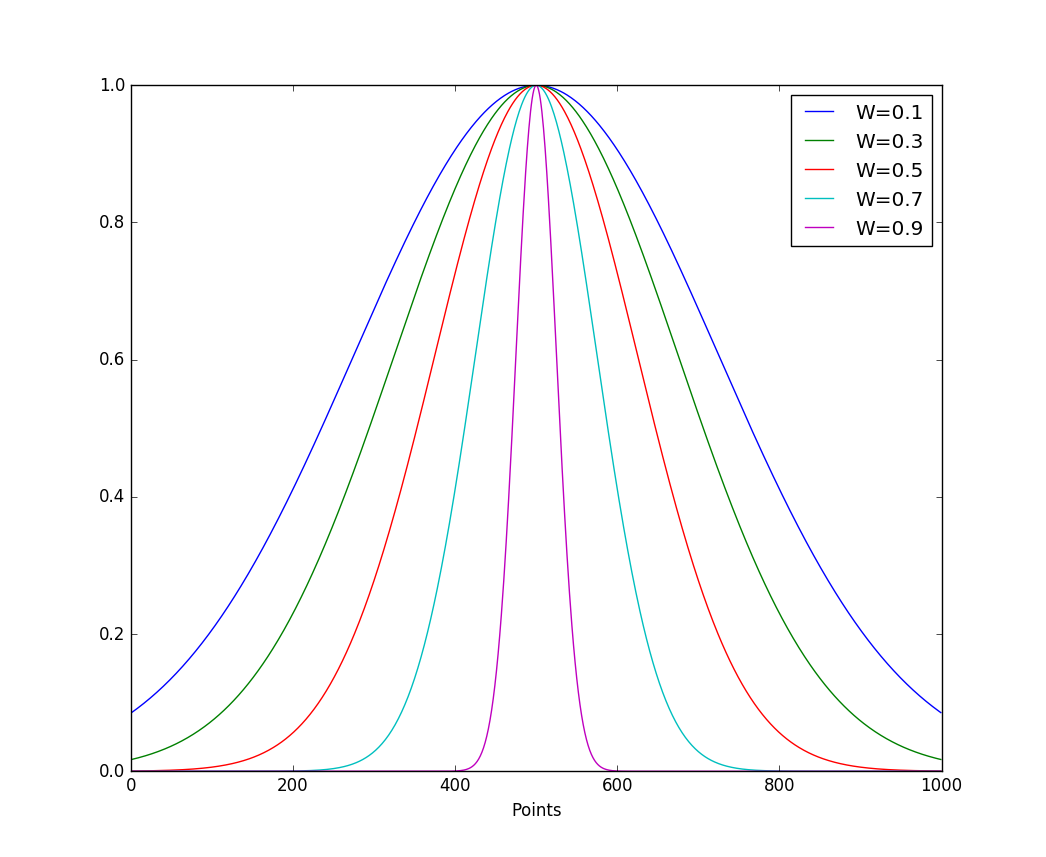
\includegraphics[scale=0.3]{./images/gaussiennes_filtre_spectral_1D.png}
\caption{Gaussienne appliqu�e � la FFT du signal en fonction du param�tre W}
\label{fig-filtre-gauss-spectral}
\end{figure}

\end{center}

%%%%%AUTEUR%%%%
\itemstyle{Auteur~:}
CNRM/GMEI/TRAMM

%%%%%REFERENCE%%%%
\itemstyle{R\'ef\'erences~:}

Utilis� dans la fili�re BASIC du LOA pour filtrer le signal lidar.
A. Mortier 2013 \cite{THESE-MORTIER-2013}.

\newpage

\section{Estimation de l'altitude de la r�tro-diffusion mol�culaire}

\itemstyle{Op\'erateur~:} \operfmt{Lidar\_Zref}
\index{Lidar\_Zref}

%%%%%OBJET%%%%
\itemstyle{Objet~:}
Pour un tir lidar vers le haut, cet op�rateur estime l'altitude � partir de laquelle
on consid�re que la r�tro-diffusion est uniquement mol�culaire. Cette altitude est utilis�e comme r�f�rence dans d'autres op�rateurs pour inverser le signal lidar.

%%%%%ARGUMENTS%%%%
\bigskip
%% Dans ce fichier, les �ventuels accents sont cod�s
%% en ISO-8859-15 (aka latin9)
%% La ligne suivante donne trois exemples 
%% e accent aigu : �, e accent grave : �, e-dans-l'o : �
%%%%%ENTREES%%%%
\begin{tabarg}
\multicolumn{3}{l}{\titretab {Entr\'ees}}\\
\hline
$X$ & Vecteur, \texttt{float[$N_{level}$]} & Signal lidar \\
$Z$ & Vecteur, \texttt{float[$N_{level}$]} & Altitudes r�elles des portes du lidar (m)\\
$Z_1$ & Coeff., \texttt{float} & Altitude minimale de la zone de recherche (m)\\
$Z_2$ & Coeff., \texttt{float} & Altitude maximale de la zone de recherche (m)\\
$N_{step}$ & Coeff., \texttt{int} & Nombre de points de la moyenne glissante de $X$ \\
\end{tabarg}



\medskip
%%%%%SORTIES%%%%
\begin{tabarg}
\multicolumn{3}{l}{\titretab {Sorties}}\\
\hline
$Z_{ref}$ & Vecteur, \texttt{float} & Altitude de r�f�rence du signal mol�culaire  (m)\\
\end{tabarg}



%%%%%FORMULE%%%%
\itemstyle{Formule}

%% Formule de l'operateur : Lidar_Zref
%% Dans ce fichier, les �ventuels accents sont cod�s
%% en ISO-8859-15 (aka latin9)
%% La ligne suivante donne trois exemples 
%% e accent aigu : �, e accent grave : �, e-dans-l'o : �

Le profil vertical du signal lidar $X$ est liss� par moyenne glissante de largeur $N_{step}$ points pour obtenir $X_{moy}$. \\
Puis on recherche le minimum de $X_{moy}$ entre les altitudes $Z_1$ et $Z_2$.\\
$Z_{ref}$ est d�termin� comme l'altitude � laquelle la diff�rence entre $X$ et $X_{moy}$ est minimale autour du minimum de $X_{moy}$.\\

%%%%%AUTEUR%%%%
\itemstyle{Auteur~:}
CNRM/GMEI/TRAMM

%%%%%REFERENCE%%%%
\itemstyle{R\'ef\'erences~:}
Fili�re BASIC du LOA. A. Mortier 2013 \cite{THESE-MORTIER-2013}.

\newpage

\section{Estimation de l'altitude de la r�tro-diffusion mol�culaire}

\itemstyle{Op\'erateur~:} \operfmt{Lidar\_Zref\_ecart}
\index{Lidar\_Zref\_ecart}

%%%%%OBJET%%%%
\itemstyle{Objet~:}
Pour un tir lidar vers le haut, cet op�rateur estime l'altitude � partir de laquelle
on consid�re que la r�tro-diffusion est uniquement mol�culaire. Cette altitude est utilis�e comme r�f�rence dans d'autres op�rateurs pour inverser le signal lidar.

%%%%%ARGUMENTS%%%%
\bigskip
%% Dans ce fichier, les �ventuels accents sont cod�s
%% en ISO-8859-15 (aka latin9)
%% La ligne suivante donne trois exemples 
%% e accent aigu : �, e accent grave : �, e-dans-l'o : �
%%%%%ENTREES%%%%
\begin{tabarg}
\multicolumn{3}{l}{\titretab {Entr\'ees}}\\
\hline
$X$ & Vecteur, \texttt{float[$N_{level}$]} & Signal lidar \\
$Z$ & Vecteur, \texttt{float[$N_{level}$]} & Altitudes r�elles des portes du lidar (m)\\
$Z_1$ & Coeff., \texttt{float} & Altitude minimale par rapport au lidar de la zone de recherche (m)\\
$Z_2$ & Coeff., \texttt{float} & Altitude maximale par rapport au lidar de la zone de recherche (m)\\
$N_{step}$ & Coeff., \texttt{int} & Nombre de points de la moyenne glissante de $X$ \\
\end{tabarg}



\medskip
%%%%%SORTIES%%%%
\begin{tabarg}
\multicolumn{3}{l}{\titretab {Sorties}}\\
\hline
$Z_{ref}$ & Vecteur, \texttt{float} & Altitude de r�f�rence du signal mol�culaire  (m)\\
\end{tabarg}



%%%%%FORMULE%%%%
\itemstyle{Formule}

%% Formule de l'operateur : Lidar_Zref
%% Dans ce fichier, les �ventuels accents sont cod�s
%% en ISO-8859-15 (aka latin9)
%% La ligne suivante donne trois exemples 
%% e accent aigu : �, e accent grave : �, e-dans-l'o : �

Le profil vertical du signal lidar $X$ est liss� par moyenne glissante de largeur $N_{step}$ points pour obtenir $X_{moy}$. \\
Puis on recherche le minimum de $X_{moy}$ entre les altitudes Z[0]+$Z_1$ et Z[0]+$Z_2$.\\
$Z_{ref}$ est d�termin� comme l'altitude � laquelle la diff�rence entre $X$ et $X_{moy}$ est minimale autour du minimum de $X_{moy}$.\\


%%%%%AUTEUR%%%%
\itemstyle{Auteur~:}
CNRM/GMEI/TRAMM

%%%%%REFERENCE%%%%
\itemstyle{R\'ef\'erences~:}
Fili�re BASIC du LOA. A. Mortier 2013 \cite{THESE-MORTIER-2013}.

\newpage
%%%%%
%
%% Dans ce fichier, les �ventuels accents sont cod�s
%% en ISO-8859-15 (aka latin9)
%% La ligne suivante donne trois exemples 
%% e accent aigu : �, e accent grave : �, e-dans-l'o : �
\section{Inversion de Klett du signal lidar en fixant le rapport lidar  }

\itemstyle{Op\'erateur~:} \operfmt{Inv\_Klett\_sa}
\index{Inv\_Klett\_sa}

%%%%%OBJET%%%%
\itemstyle{Objet~:}
Calcul du profil de r�trodiffusion des a�rosols et de l'AOD par inversion de Klett � partir du signal lidar en fixant le rapport lidar.

%%%%%ARGUMENTS%%%%
\bigskip
%% Dans ce fichier, les �ventuels accents sont cod�s
%% en ISO-8859-15 (aka latin9)
%% La ligne suivante donne trois exemples 
%% e accent aigu : �, e accent grave : �, e-dans-l'o : �
%%%%%ENTREES%%%%
\begin{tabarg}
\multicolumn{3}{l}{\titretab {Entr\'ees}}\\
\hline
$X$ & Vecteur, \texttt{float[$N_{level}$]} & Signal lidar \\
$Z$ & Vecteur, \texttt{float[$N_{level}$]} & Altitudes r�elles des portes du lidar (m)\\
$\beta_{mol}$ & Vecteur, \texttt{float[$N_{level}$]} &  Profil du coefficient de r�tro-diffusion mol�culaire ($m^{-1}$)\\
$Alt_{nuage}$ & Vecteur, \texttt{float} & Altitude des nuages (vaut 0 si pas de nuage) (m)\\
$Z_{ref}$ & Vecteur, \texttt{float} & Altitude de r�f�rence pour le signal mol�culaire (m)\\
$D_{min}$ & Coeff., \texttt{float} & Distance minimale du lidar � partir de laquelle on d�termine le profil (m)\\
$\beta_{ainit}$ & Coeff., \texttt{float} & Valeur d'initialisation de $\beta$  ($m^{-1}$)\\
$SA$ & Coeff., \texttt{float} & Rapport lidar \\
$Extrap$ & Coeff., \texttt{String} & Type d'extrapolation pour la zone proche du lidar (< $D_{min}$) :"lin" ou "cst" \\
\end{tabarg}

\medskip
%%%%%SORTIES%%%%
\begin{tabarg}
\multicolumn{3}{l}{\titretab {Sorties}}\\
\hline
$\beta$ & Vecteur, \texttt{float[$N_{level}$]} & Coefficient de r�tro-diffusion des a�rosols (m-1)\\
$AOD$ & Vecteur, \texttt{float} & Epaisseur optique des a�rosols\\
\end{tabarg}



%%%%%FORMULE%%%%
\itemstyle{Formule}

%% Formule de l'operateur : Inv_Klett_sa
%% Dans ce fichier, les �ventuels accents sont cod�s
%% en ISO-8859-15 (aka latin9)
%% La ligne suivante donne trois exemples 
%% e accent aigu : �, e accent grave : �, e-dans-l'o : �

\bigskip
A chaque pas de temps : \\

Si $Alt_{nuage} \leq Z_{ref}$ et $Alt_{nuage} \neq 0$  alors : \\
\begin{align*}
\beta(Z) & = valeur manquante\\
AOD & = valeur manquante
\end{align*}
\bigskip
sinon :
\begin{align*}
I_1(Z)  & = 2.(SA -S_{mol}).\left( \sum_0^{Z_{ref}} \beta_{mol}(z_j) .\Delta z_j - \sum_0^{Z} \beta_{mol}(z_j) .\Delta z_j \right) \\
\phi(z) & = \ln \left( \frac{X(Z)}{X(Z_{ref})} \right) + I_1(Z) \\ 
I_2(Z) & = 2.SA.\left(\sum_0^{Z_{ref}} \exp(\phi(z_j)).\Delta z_j - \sum_0^{Z} \exp(\phi(z_j)).\Delta z_j \right) \\
\beta (Z) & = \frac{\exp(\phi(Z))}{1/\beta(Z_{ref}) + I_2(Z) } \\
AOD & = \sum_0^{Z_{ref}} SA*\beta(z_j).\Delta z_j  
\end{align*}

avec :
\begin{align*}
S_{mol} &  =   8.\pi /3 \\
\beta(Z_{ref}) & = \beta_{mol}(Z_{ref}) + \beta_{ainit}
\end{align*}


%%%%%AUTEUR%%%%
\itemstyle{Auteur~:}
CNRM/GMEI/TRAMM

%%%%%REFERENCE%%%%
\itemstyle{R\'ef\'erences~:}
Fili�re BASIC du LOA. 

\newpage
%%%%%
%
%% Dans ce fichier, les �ventuels accents sont cod�s
%% en ISO-8859-15 (aka latin9)
%% La ligne suivante donne trois exemples 
%% e accent aigu : �, e accent grave : �, e-dans-l'o : �
\section{Inversion de Klett du signal lidar avec AOD donn�}

\itemstyle{Op\'erateur~:} \operfmt{Inv\_Klett\_aod}
\index{Inv\_Klett\_aod}

%%%%%OBJET%%%%
\itemstyle{Objet~:}
Calcul du profil de r�trodiffusion et d'absorption des a�rosols  par inversion de Klett � partir du signal lidar et de l'AOD.

%%%%%ARGUMENTS%%%%
\bigskip
%% Dans ce fichier, les �ventuels accents sont cod�s
%% en ISO-8859-15 (aka latin9)
%% La ligne suivante donne trois exemples 
%% e accent aigu : �, e accent grave : �, e-dans-l'o : �
%%%%%ENTREES%%%%
\begin{tabarg}
\multicolumn{3}{l}{\titretab {Entr\'ees}}\\
\hline

$X$ & Vecteur, \texttt{float[$N_{level}$]} & Signal lidar \\
$Z$ & Vecteur, \texttt{float[$N_{level}$]} & Altitudes r�elles des portes du lidar (m)\\
$\beta_{mol}$ & Vecteur, \texttt{float[$N_{level}$]} &  Profil du coefficient de r�tro-diffusion mol�culaire ($m^{-1}$)\\
$Alt_{nuage}$ & Vecteur, \texttt{float} & Altitude des nuages (vaut 0 si pas de nuage) (m)\\
$AOD$ & Vecteur, \texttt{float} & Epaisseur optique des a�rosols\\
$Z_{ref}$ & Vecteur, \texttt{float} & Altitude de r�f�rence pour le signal mol�culaire (m)\\
$D_{min}$ & Vecteur, \texttt{float} & Distance minimale du lidar � partir de laquelle on d�termine le profil (m)\\
$\beta_{ainit}$ & Coeff., \texttt{float} & Valeur d'initialisation de $\beta$  ($m^{-1}$)\\
$Extrap$ & Coeff., \texttt{String} & Type d'extrapolation pour la zone proche du lidar (< $D_{min}$) :"lin" ou "cst" \\
\end{tabarg}

\medskip
%%%%%SORTIES%%%%
\begin{tabarg}
\multicolumn{3}{l}{\titretab {Sorties}}\\
\hline
$\sigma$ & Vecteur, \texttt{float[$N_{level}$]} & Coefficient d'extinction des a�rosols (m-1)\\
$\beta$ & Vecteur, \texttt{float[$N_{level}$]} & Coefficient de r�tro-diffusion des a�rosols (m-1)\\
$SA$ & Vecteur, \texttt{float} & Rapport lidar\\
\end{tabarg}



%%%%%FORMULE%%%%
\itemstyle{Formule}

%% Formule de l'operateur : Inv_Klett_aod
%% Dans ce fichier, les �ventuels accents sont cod�s
%% en ISO-8859-15 (aka latin9)
%% La ligne suivante donne trois exemples 
%% e accent aigu : �, e accent grave : �, e-dans-l'o : �

\bigskip
A chaque pas de temps : \\

Si $Alt_{nuage} \leq Z_{ref}$ et $Alt_{nuage} \neq 0$  alors : \\
\begin{align*}
\beta(Z) & = valeur\ manquante\\
\sigma(Z) & = valeur\ manquante\\
SA & = valeur\ manquante
\end{align*}
\bigskip
sinon on cherche  par it�rations successives la valeur de $SA$ pour laquelle l'$AOD_{calcule}$ calcul� ci-dessous est le plus proche de l'$AOD$ donn�. La tol�rance sur $SA$ est de 0.1. 
\begin{align*}
I_1(Z)  & = 2.(SA -S_{mol}).\left( \sum_0^{Z_{ref}} \beta_{mol}(z_j) .\Delta z_j - \sum_0^{Z} \beta_{mol}(z_j) .\Delta z_j \right) \\
\phi(z) & = \ln \left( \frac{X(Z)}{X(Z_{ref})} \right) + I_1(Z) \\ 
I_2(Z) & = 2.SA.\left(\sum_0^{Z_{ref}} \exp(\phi(z_j)).\Delta z_j - \sum_0^{Z} \exp(\phi(z_j)).\Delta z_j \right) \\
\beta (Z) & = \frac{\exp(\phi(Z))}{1/\beta(Z_{ref}) + I_2(Z) } \\
AOD_{calcule} & = \sum_0^{Z_{ref}} SA*\beta(z_j).\Delta z_j \\
\sigma (Z) & = SA*\beta(Z)
\end{align*}

avec :
\begin{align*}
S_{mol} &  =   8.\pi /3 \\
\beta(Z_{ref}) & = \beta_{mol}(Z_{ref}) + \beta_{ainit}
\end{align*}





%%%%%AUTEUR%%%%
\itemstyle{Auteur~:}
CNRM/GMEI/TRAMM

%%%%%REFERENCE%%%%
\itemstyle{R\'ef\'erences~:}
Fili�re BASIC du LOA. 

\newpage
%%%%%
%
%% Dans ce fichier, les �ventuels accents sont cod�s
%% en ISO-8859-15 (aka latin9)
%% La ligne suivante donne trois exemples 
%% e accent aigu : �, e accent grave : �, e-dans-l'o : �
\section{Estimation des hauteurs et bases de nuage � partir d'un profil lidar}

\itemstyle{Op\'erateur~:} \operfmt{Nuage\_lidar}
\index{Nuage\_lidar}

%%%%%OBJET%%%%
\itemstyle{Objet~:}
Cet op�rateur d�termine la hauteur des bases et sommets des nuages par une m�thode mise au point par A. Mortier 2013 \cite{THESE-MORTIER-2013} et inspir�e de Pal et al. (1992). 

%%%%%ARGUMENTS%%%%
\bigskip
%% Dans ce fichier, les �ventuels accents sont cod�s
%% en ISO-8859-15 (aka latin9)
%% La ligne suivante donne trois exemples 
%% e accent aigu : �, e accent grave : �, e-dans-l'o : �
%%%%%ENTREES%%%%
\begin{tabarg}
\multicolumn{3}{l}{\titretab {Entr\'ees}}\\
\hline
$X$ & Vecteur, \texttt{float[$N_{level}$]} & Signal lidar \\
$S_1$ & Coeff., \texttt{int} & Seuil de d�tection \\
$S_2$ & Coeff., \texttt{int} & Seuil de d�tection \\
$Z$ & Vecteur, \texttt{float[$N_{level}$]} & Altitudes r�elles des portes du lidar (m)\\
$Z_{min}$ & Coeff., \texttt{int} & Altitude en dessous de laquelle on ne d�tecte pas de nuage (m)\\
\end{tabarg}

\medskip
%%%%%SORTIES%%%%
\begin{tabarg}
\multicolumn{3}{l}{\titretab {Sorties}}\\
\hline
$Base$ & Vecteur, \texttt{float[6]} & Altitude des bases des nuages (m)\\
$Max$ & Vecteur, \texttt{float[6]} & Altitude des maximums de r�tro-diffusion (m)\\
$Sommet$ & Vecteur, \texttt{float[6]} & Altitude des sommets des nuages (m)\\
$Flag_{nuage}$ & Vecteur, \texttt{float} & Nombre de couches d�tect�es (m)\\
\end{tabarg}



%%%%%FORMULE%%%%
\itemstyle{Formule}

%% Formule de l'operateur : Nuage_lidar
%% Dans ce fichier, les �ventuels accents sont cod�s
%% en ISO-8859-15 (aka latin9)
%% La ligne suivante donne trois exemples 
%% e accent aigu : �, e accent grave : �, e-dans-l'o : �


L'algorithme est d�crit dans la th�se cit�e en r�f�rence dans la partie 2.3.4.2. Il est bas� sur la variabilit� verticale de chaque profil. Les minimuns et maximums du profil sont dans un premier temps d�termin�s � partir de la d�riv�e du profil. Puis ces valeurs sont s�lectionn�es en fonction des 2 seuils $S_1$ et $S_2$.\\
Pour qu'un nuage soit identifi� il faut que : \\
\begin{itemize}
\item la diff�rence du signal lidar entre le maximum et la base d�tect�s soit sup�rieur � $S_1$ fois le bruit du signal 
\item le rapport de signal lidar entre le maximum et le sommet du nuage d�tect� soit sup�rieur � $S_2$.
\end{itemize}
Les valeurs recommand�es pour les seuils de d�tection sont $S_1= 10$ et $S_2=4$.

 

%%%%%AUTEUR%%%%
\itemstyle{Auteur~:}
CNRM/GMEI/TRAMM

%%%%%REFERENCE%%%%
\itemstyle{R\'ef\'erences~:}
Utilis� dans la fili�re BASIC du LOA, A. Mortier 2013 \cite{THESE-MORTIER-2013}.

\newpage
%%%%%
%
%% Dans ce fichier, les �ventuels accents sont cod�s
%% en ISO-8859-15 (aka latin9)
%% La ligne suivante donne trois exemples 
%% e accent aigu : �, e accent grave : �, e-dans-l'o : �
\section{Calcul de la hauteur de la couche limite atmosph�rique � partir des donn�es lidar/t�l�m�tre}

\itemstyle{Op\'erateur~:} \operfmt{Hauteur\_CL\_Lidar}
\index{Calcul\_CL\_Lidar}

%%%%%OBJET%%%%
\itemstyle{Objet~:}
Calcul de la hauteur de la couche limite par d�tection de gradient par la m�thode de l'ondelette de Haar.

%%%%%ARGUMENTS%%%%
\bigskip
%% Dans ce fichier, les �ventuels accents sont cod�s
%% en ISO-8859-15 (aka latin9)
%% La ligne suivante donne trois exemples 
%% e accent aigu : �, e accent grave : �, e-dans-l'o : �
%%%%%ENTREES%%%%
\begin{tabarg}
\multicolumn{3}{l}{\titretab {Entr\'ees}}\\
\hline
$PR2$ & Vecteur, \texttt{float} &  Signal r�trodiffus�\\
$base\_cld$ & Vecteur, \texttt{float} & Hauteur de base des nuages\\
$width\_wave$ & Coeff., \texttt{float} & Epaisseur de l'ondelette \\
$thr\_cloud$ & Coeff., \texttt{float} & Seuil nuage \\
$zmin_bl$ & Coeff., \texttt{float} & Altitude min de la HCLA \\
$zmax_bl$ & Coeff., \texttt{float} & Altitude max de la HCLA \\
$zmax_tl$ & Coeff., \texttt{float} & Altitude max de la TL \\
\end{tabarg}

\medskip
%%%%%SORTIES%%%%
\begin{tabarg}
\multicolumn{3}{l}{\titretab {Sorties}}\\
\hline
$z_bl$ & Vecteur, \texttt{float} & Hauteur de couche limite atmosph�rique\\
$z_tl$ & Vecteur, \texttt{float} & Hauteur de la TL\\
\end{tabarg}


%%%%%AUTEUR%%%%
\itemstyle{Auteur~:}
CNRM/GMEI/TRAMM

%%%%%REFERENCE%%%%
\itemstyle{R\'ef\'erences~:}
BASIC

\newpage
%%%%%
%
%% Dans ce fichier, les �ventuels accents sont cod�s
%% en ISO-8859-15 (aka latin9)
%% La ligne suivante donne trois exemples 
%% e accent aigu : �, e accent grave : �, e-dans-l'o : �
\section{Indicateur de qualit� du signal lidar}

\itemstyle{Op\'erateur~:} \operfmt{Qualite\_profil\_lidar}
\index{Qualite\_profil\_lidar}

%%%%%OBJET%%%%
\itemstyle{Objet~:}
Calcul d'un indicateur de qualit� du signal lidar par rapport � la r�tro-diffusion mol�culaire.

%%%%%ARGUMENTS%%%%
\bigskip
%% Dans ce fichier, les �ventuels accents sont cod�s
%% en ISO-8859-15 (aka latin9)
%% La ligne suivante donne trois exemples 
%% e accent aigu : �, e accent grave : �, e-dans-l'o : �
%%%%%ENTREES%%%%
\begin{tabarg}
\multicolumn{3}{l}{\titretab {Entr\'ees}}\\
\hline
$X$ & Vecteur, \texttt{float[$N_{level}$]} & Signal lidar \\
$X_{mol}$ & Vecteur, \texttt{float[$N_{level}$]} & Signal de r�tro-diffusion mol�culaire \\
$Z$ & Vecteur, \texttt{float[$N_{level}$]} & Altitudes r�elles des portes du lidar (m)\\
$Z_{ref}$ & Vecteur, \texttt{float} & Altitude de r�f�rence du signal mol�culaire  (m)\\
\end{tabarg}

\medskip
%%%%%SORTIES%%%%
\begin{tabarg}
\multicolumn{3}{l}{\titretab {Sorties}}\\
\hline
$Q$ & Vecteur, \texttt{float} & Indicateur de qualit� du profil lidar \\
\end{tabarg}



%%%%%FORMULE%%%%
\itemstyle{Formule}

%% Formule de l'operateur : Qualite_profil_lidar
%% Dans ce fichier, les �ventuels accents sont cod�s
%% en ISO-8859-15 (aka latin9)
%% La ligne suivante donne trois exemples 
%% e accent aigu : �, e accent grave : �, e-dans-l'o : �

Cet op�rateur calcule la pente du signal lidar $X$ dans une tranche d'altitude de 1500 m d'�paisseur autour de l'altitude $Z_{ref}$. Le rapport de cette pente et de celle du signal mol�culaire $X_{mol}$ repr�sente la qualit� du signal $Q$.



%%%%%AUTEUR%%%%
\itemstyle{Auteur~:}
CNRM/GMEI/TRAMM

%%%%%REFERENCE%%%%
\itemstyle{R\'ef\'erences~:}
Utilis� dans la fili�re BASIC du LOA.
A. Mortier 2013 \cite{THESE-MORTIER-2013}.

\newpage
\chapter{D�tection et corrections d'�chantillons inhomog�nes}

%%%%%
%
\section{Correction de sauts dans le temps acquis par le Merlin IV}

\itemstyle{Op\'erateur~:} {\sf correc\_time\_rec}

%%%%%OBJET%%%%
\itemstyle{Objet~:}
Correction des sauts anormaux dans le temps acquis par le
syst\`eme d'acquisition du Merlin IV. 

%%%%%ARGUMENTS%%%%
\bigskip
%%%%%ENTREES%%%%
\begin{tabarg}
\multicolumn{3}{l}{\titretab {Entr\'ees}}\\
\hline
$Time$ & Vecteur, {\tt double} & Temps ($s$)\\
$f_e$ & Coeff., {\tt float} & Fr\'equence d'\'echantillonnage ($Hz$)\\
\end{tabarg}

\medskip
%%%%%SORTIES%%%%
\begin{tabarg}
\multicolumn{3}{l}{\titretab {Sorties}}\\
\hline
$Time_c$ & Vecteur, {\tt double} & Temps corrig\'e ($s$)\\
\end{tabarg}


%%%%%FORMULE%%%%
\itemstyle{Formule}

%%correc_time_rec
Correction des sauts de $Time$.


%%%% COMMENTAIRE %%%%
\itemstyle{Commentaire~:}

En principe, le temps cro\^{\i}t r\'eguli\`erement
de $1/f_e \pm \varepsilon $ \`a chaque instant.
Mais, il peut se produire des "sauts" ou des "trous".
Un "saut" est constitu\'e par N valeurs 
cons\'ecutives "incorrectes". 
Un "trou" est l'absence de N valeurs 
cons\'ecutives dans la s\'erie. \\
L'algorithme remplace les valeurs "incorrectes" des
"sauts" et ne touche pas les "trous".\\
$\varepsilon$ est l'incertitude sur le temps du
syst\`eme d'acquisition. Elle doit \^etre ici
inf\'erieure \`a $6.10^{-4} s$ ( sp\'ecifique au
Merlin IV) pour que la valeur soit consid\'er\'ee
correcte.
Un "saut" ne peut pas durer plus de 20 valeurs
cons\'ecutives sinon il est consid\'er\'e 
comme un "trou".


%%%%%AUTEUR%%%%
\itemstyle{Auteur~:}
CNRM/GMEI/TRAMM

%%%%%REFERENCE%%%%
\itemstyle{R\'ef\'erences~:}

\newpage
%%%%%
%
\section{Correction de sauts simples}

\itemstyle{Op\'erateur~:} \operfmt{correc\_saut}
\index{correc\_saut}

%%%%%OBJET%%%%
\itemstyle{Objet~:}
D\'etection de sauts sup\'erieur \`a un seuil 
se produisant sur une seule valeur. La valeur "fausse"
est remplac\'ee par la moyenne des valeurs qui l'encadrent. 

%%%%%ARGUMENTS%%%%
\bigskip
%%%%%ENTREES%%%%
\begin{tabarg}
\multicolumn{3}{l}{\titretab {Entr\'ees}}\\
\hline
$X$ & Vecteur, \texttt{float} & Param\`etre d'entr\'ee \\
$S_0$ & Coeff., \texttt{float} & Seuil de d\'etection d'un saut (m\^eme unit� que $X$, et doit
\^etre positif)\\
\end{tabarg}

\medskip
%%%%%SORTIES%%%%
\begin{tabarg}
\multicolumn{3}{l}{\titretab {Sorties}}\\
\hline
$X_c$ & Vecteur, \texttt{float} & Param\`etre corrig\'e (m\^eme unit\'e que $X$)\\
\end{tabarg}


%%%%%FORMULE%%%%
\itemstyle{Formule}

%%correc_saut
L'\'echantillon de rang $i$ est consid\'er\'e comme un saut si :
$|X[i] - X[i-1]| > S_0$ et $|X[i] - X[i+1]| > S_0$  et $ (X[i] - X[i - 1]) * (X[i] - X[i + 1]) > 0$ 

alors $X_c[i] = \frac{X[i+1] + X[i-1]}{2}$ . Sinon, $X_c[i] = X[i]$


%%%%%COMMENTAIRES%%%%
\itemstyle{Commentaires}

\emph{Attention} : L'interpolation lin�aire ne convient pas aux variables
qui peuvent �tre naturellement discontinues, tels les caps et
autres angles.

%%%%%AUTEUR%%%%
\itemstyle{Auteur~:}
CNRM/GMEI/TRAMM

%%%%%REFERENCE%%%%
\itemstyle{R\'ef\'erences~:}

\newpage
%%%%%
%
%% Dans ce fichier, les �ventuels accents sont cod�s
%% en ISO-8859-15 (aka latin9)
%% La ligne suivante donne trois exemples 
%% e accent aigu : �, e accent grave : �, e-dans-l'o : �
\section{Correction de pics simples avec prise en compte des valeurs manquantes}

\itemstyle{Op\'erateur~:} \operfmt{Correc\_pics\_mnq}
\index{Correc\_pics\_mnq}

%%%%%OBJET%%%%
\itemstyle{Objet~:}
D�tection de pics sup�rieurs � un seuil se produisant sur une seule valeur. La valeur
"fausse" est �ventuellement remplac�e par la moyenne des valeurs qui l'encadrent en fonction du param�tre $N_r$ en entr�e. La d�tection de pics se fait aussi avant ou apr�s des valeurs manquantes.

%%%%%ARGUMENTS%%%%
\bigskip
%% Dans ce fichier, les �ventuels accents sont cod�s
%% en ISO-8859-15 (aka latin9)
%% La ligne suivante donne trois exemples 
%% e accent aigu : �, e accent grave : �, e-dans-l'o : �
%%%%%ENTREES%%%%
\begin{tabarg}
\multicolumn{3}{l}{\titretab {Entr\'ees}}\\
\hline
$X$ & Vecteur, \texttt{float} & Param�tre d'entr�e\\
$S_0$ & Coeff., \texttt{float} & Seuil de d�tection d'un pic\\
$S_{mnq}$ & Coeff., \texttt{float} & Seuil de d�tection d'un saut avant ou apr�s une valeur manquante \\
$N_r$ & Coeff., \texttt{float} & Nombre maximum de points invalid�s � remplacer par une interpolation lin�aire\\
\end{tabarg}

\medskip
%%%%%SORTIES%%%%
\begin{tabarg}
\multicolumn{3}{l}{\titretab {Sorties}}\\
\hline
$Flag$ & Vecteur, \texttt{float} & Flag de diagnostic de la correction des pics \\
$X_c$ & Vecteur, \texttt{float} & Param�tre corrig� (m�me unit� que $X$)\\
\end{tabarg}


%%%%%FORMULE%%%%
\itemstyle{Formule}

%% Formule de l'operateur : Correc_pics_mnq
%% Dans ce fichier, les �ventuels accents sont cod�s
%% en ISO-8859-15 (aka latin9)
%% La ligne suivante donne trois exemples 
%% e accent aigu : �, e accent grave : �, e-dans-l'o : �

A chaque instant $j$ :
\begin{itemize}
\item un pic est d\'etect\'e si : \newline
$X[j] - X[j-1] > S_0$ et $X[j] - X[j+1] > S_0$  (pic vers le haut)

ou 

$X[j-1] - X[j] > S_0$ et $X[j+1] - X[j] > S_0$  (pic vers le bas)

\hspace*{1cm} alors $flag[j] = 1$ si pic vers le haut, ou $flag[j] = -1$ si 
pic vers le bas \newline

Dans ce cas si le nombre de pics d�tect�s $\leq N_r$ alors $X_c[j]$ est remplac� par une interpolation lin�aire entre les valeurs valides, sinon $X_c[j]$ = mnq \newline

\item un saut apr�s une valeur manquante est d\'etect\'e si :\newline
$X[j-1] = mnq$
et
$|X[j+1] - X[j]| > S_{mnq}$ 

\hspace*{1cm} alors $flag[j] = 3$  si saut vers le haut, ou $flag[j] = -3$ si 
pic vers le bas 
et $X_c[j] = mnq$ \newline

\item un saut avant une valeur manquante est d\'etect\'e si :\newline
$X[j+1] = mnq$
et
$|X[j] - X[j-1]| > S_{mnq}$ 

\hspace*{1cm} alors $flag[j] = 2$ si saut vers le haut, ou $flag[j] = -2$ si 
saut vers le bas$X_c[j] = X[j]$ \newline

\item une forte variation positive est d\'etect\'e si :\newline
$X[j+1] - X[j] > S_0$ et $X[j] - X[j-1] > S_0$  (forte variation vers le haut)

\hspace*{1cm} alors $flag[j] = 4$ et  $X_c[j] = X[j]$ \newline

\item une forte variation n�gative est d\'etect\'e si :\newline
$X[j-1] - X[j] > S_0$ et $X[j] - X[j+1] > S_0$  (forte variation vers le bas)

\hspace*{1cm} alors $flag[j] = -4$ et $X_c[j] = X[j]$ \newline

\item aucune variation "particuli�re" n'est d�tect�e :\newline
\hspace*{1cm} alors $flag[j] = 0$ et $X_c[j] = X[j]$ \newline

\end{itemize}





%%%%%COMMENTAIRES%%%%
\itemstyle{Commentaires :}

Cet op�rateur remplace l'op�rateur  \operfmt{correc\_saut\_mnq}. \\
Il am�liore :
\begin{itemize}
\item  le traitements de tous les cas de sauts avant ou apr�s une valeur manquante
\item l'interpolation lin�aire en cas de pics successifs
\item la prise en compte du seuil de dur�e max ($N_r$) pour l'interpolation lin�aire ( il ne remplace pas les valeurs d�j� manquantes dans $X$)
\end{itemize}
\bigskip 

\emph{Attention} : L'interpolation lin�aire ne convient pas aux variables
qui peuvent �tre naturellement discontinues, tels les caps et
autres angles.





%%%%%AUTEUR%%%%
\itemstyle{Auteur~:}
CNRM/GMEI/TRAMM

%%%%%REFERENCE%%%%
\itemstyle{R\'ef\'erences~:}


\newpage
%%%%%
%
\section{Correction de pics isol�s dans une s�rie de valeurs modulaires}

\itemstyle{Op\'erateur~:} \operfmt{correc\_pics\_angle\_auto\_unit}
\index{correc\_pics\_angle\_auto\_unit}

%%%%%OBJET%%%%
\itemstyle{Objet~:}
Les pics isol�s sont d�finis comme les �chantillons dont
les �carts au pr�c�dant et au suivant sont 
de signe oppos�s, et sup�rieurs (en valeur absolue)
� un certain seuil. 

Cet op�rateur d�tecte les pics dans une s�rie de
donn�es, et les remplace par une interpolation entre
les valeurs contigu�s.

Cet op�rateur est adapt� au cas des variables d�finies sur un domaine
p�riodique (arithm�thiqe modulaire), typiquement les angles : la 
transition entre 359 degr�s et 1 degr� n'est pas consid�r�e comme 
une discontinuit�.


%%%%%ARGUMENTS%%%%
\bigskip
%%%%%ENTREES%%%%
\begin{tabarg}
\multicolumn{3}{l}{\titretab {Entr\'ees}}\\
\hline
$X$ & Vecteur, \texttt{float} & S�rie de donn�es originelle \\
$S_0$ & Coeff., \texttt{float} & Seuil de d\'efinition d'un saut (m\^eme unit� que $X$, doit
\^etre positif et inf�rieur � la moiti� du domaine de p�riodicit�)\\
unit & Coeff., \texttt{string} & unit� de $X$ (degr�s ou radian)\\
\end{tabarg}

\medskip
%%%%%SORTIES%%%%
\begin{tabarg}
\multicolumn{3}{l}{\titretab {Sorties}}\\
\hline
$X_c$ & Vecteur, \texttt{float} & S�rie corrig�e (m\^eme unit\'e que $X$)\\
\end{tabarg}


%%%%%FORMULE%%%%
\itemstyle{Formule}

%% correc_pics_angle_auto_unit
L'\'echantillon $i$ est consid\'er\'e comme un saut si :


$|X[i] - X[i-1]| > S_0$ et $|X[i] - X[i+1]| > S_0$  et $ (X[i] - X[i - 1]) * (X[i] - X[i + 1]) > 0$


%%%%%AUTEUR%%%%
\itemstyle{Auteur~:}
CNRM/GMEI/TRAMM

%%%%%REFERENCE%%%%
\itemstyle{R\'ef\'erences~:}

\newpage
%%%%%
%
\section{Correction de valeurs hors-bornes}

\itemstyle{Op\'erateur~:} {\sf Correc\_hors\_bornes}
\index{Correc\_hors\_bornes}

%%%%%OBJET%%%%
\itemstyle{Objet~:}
Cette fonction d�tecte et remplace les valeurs hors d'un intervalle
sp�cifi�. Si la dur�e des valeurs fausses cons�cutives est courte
(inf�rieure � un seuil fix�), elles sont remplac�es par interpolation
lin�aire. Dans le cas contraire, elles sont marqu�es  comme des
�valeurs manquantes�.

%%%%%ARGUMENTS%%%%
\bigskip
%%%%%ENTREES%%%%
\begin{tabarg}
\multicolumn{3}{l}{\titretab {Entr\'ees}}\\
\hline
$X$ & Vecteur, \texttt{float} & Param�tre\\
$borne_{inf}$ & Coeff., \texttt{float} & Valeur min. permise\\
$borne_{sup}$ & Coeff., \texttt{float} & Valeur max. permise\\
$seuil_{duree}$ & Coeff., \texttt{int} & Nombre maxi de valeurs cons�cutives\\
$MisVal$ & Coeff., \texttt{float} & Valeur sp�ciale pour donn�e absente.\\
\end{tabarg}

\medskip
%%%%%SORTIES%%%%
\begin{tabarg}
\multicolumn{3}{l}{\titretab {Sorties}}\\
\hline
$X_{cor}$ & Vecteur, \texttt{float} & Param�tre corrig� (m�me unit� que $X$)\\
\end{tabarg}


%%%%%FORMULE%%%%
\itemstyle{Formule}

%%Correc_hors_bornes
1- recherche de p�riodes de valeurs hors-bornes cons�cutives.\newline
2- Pour chaque p�riode :\newline
\indent Si elle est de dur�e $< seuil_{duree}$, et encadr�e par 
des valeurs correctes,\newline
\hspace*{2cm} remplacement par une interpolation lin�aire\newline
sinon\newline
\hspace*{2cm} remplacement par des �valeurs manquantes�.


%%%%%COMMENTAIRE%%%%
\itemstyle{Commentaire~:}
L'interpolation lin�aire ne convient pas aux variables
qui peuvent �tre naturellement discontinues, tels les caps et
autres angles.

%%%%%AUTEUR%%%%
\itemstyle{Auteur~:}
CNRM/GMEI/TRAMM

%%%%%REFERENCE%%%%
\itemstyle{R\'ef\'erences~:}


\newpage
%%%%%
%
\section{Correction de valeurs hors-bornes avec flag}

\itemstyle{Op\'erateur~:} {\sf Correc\_hors\_bornes\_flag}
\index{Correc\_hors\_bornes\_flag}

%%%%%OBJET%%%%
\itemstyle{Objet~:}
Cette fonction d�tecte et remplace les valeurs hors d'un intervalle
sp�cifi�. Si la dur�e des valeurs fausses ou manquantes cons�cutives est courte
(inf�rieure � un seuil fix�), elles sont remplac�es par interpolation
lin�aire. Dans le cas contraire, la valeur en sortie est manquante.

Une variable flag indique si la valeur d'origine est valide,
manquante ou hors bornes.

%%%%%ARGUMENTS%%%%
\bigskip
%%%%%ENTREES%%%%
\begin{tabarg}
\multicolumn{3}{l}{\titretab {Entr\'ees}}\\
\hline
$X$ & Vecteur, \texttt{float} & param�tre\\
$borne_{inf}$ & Coeff., \texttt{float} & valeur min. admise\\
$borne_{sup}$ & Coeff., \texttt{float} & valeur max. admise\\
$seuil_{duree}$ & Coeff., \texttt{int} & Nombre maxi de valeurs cons�cutives\\
$MisVal$ & Coeff., \texttt{float} & valeur sp�ciale pour donn�e absente\\
\end{tabarg}

\medskip
%%%%%SORTIES%%%%
\begin{tabarg}
\multicolumn{3}{l}{\titretab {Sorties}}\\
\hline
$flag$ & Vecteur, \texttt{float} & flag en fonction de la valeur du parametre $X$ [-10, -1, 0, 1]\\
$X_{cor}$ & Vecteur, \texttt{float} & param�tre corrig� (m�me unit� que $X$)\\
\end{tabarg}


%%%%%FORMULE%%%%
\itemstyle{Formule}

%%Correc_hors_bornes_flag
1- recherche de p�riodes de valeurs hors-bornes cons�cutives.\newline
2- Pour chaque p�riode :\newline
\indent Si elle est de dur�e $< seuil_{duree}$, et encadr�e par 
des valeurs correctes,\newline
\hspace*{2cm} remplacement par une interpolation lin�aire\newline
sinon\newline
\hspace*{2cm} remplacement par des �valeurs manquantes�.\newline
\newline
En sortie : le flag permet de conna�tre l'origine des valeurs :
\begin{description}
\item[ ~0] si la valeur initiale $X$ est valide (non manquante et comprise entre les 2 bornes fix�es)
\item[ -1] si la valeur initiale $X$ est inf�rieure � la borne minimale
\item[ +1] si la valeur initiale $X$ est sup�rieure � la borne maximale
\item[-10] si la valeur initiale est manquante
\end{description}



%%%%%COMMENTAIRE%%%%
\itemstyle{Commentaire~:}
\begin{itemize}
\item Cette fonction est identique � Correc\_hors\_bornes avec l'ajout
d'un flag en sortie.
\item L'interpolation lin�aire ne convient pas aux variables
qui peuvent �tre naturellement discontinues, tels les caps et
autres angles.
\item Le flag peut s'utiliser de la fa�on suivante : si le flag
est nul, la valeur n'a pas �t� modifi�e (non interpol�e et non manquante).
\end{itemize}

%%%%%AUTEUR%%%%
\itemstyle{Auteur~:}
CNRM/GMEI/TRAMM

%%%%%REFERENCE%%%%
\itemstyle{R\'ef\'erences~:}


\newpage
%%%%%
%
\section{Remplacement de valeurs hors-bornes}

\itemstyle{Op\'erateur~:} {\sf Remplace\_hors\_bornes}
\index{Remplace\_hors\_bornes}

%%%%%OBJET%%%%
\itemstyle{Objet~:}
Cette fonction remplace les valeurs d'un vecteur qui sont hors d'un
intervalle sp�cifi� par les valeurs d'un autre vecteur (en g�n�ral
le r�sultat d'un calcul estimatif).

%%%%%ARGUMENTS%%%%
\bigskip
%%%%%ENTREES%%%%
\begin{tabarg}
\multicolumn{3}{l}{\titretab {Entr\'ees}}\\
\hline
$X$ & Vecteur, \texttt{float} & S�rie d'origine (unit� indiff�rente)\\
$borne_{inf}$ & Coeff., \texttt{float} & Valeur min. permise\\
$borne_{sup}$ & Coeff., \texttt{float} & Valeur max. permise\\
$X_{rempla}$  & Vecteur, \texttt{float} & S�rie de remplacement (m�me unit� que $X$)\\
\end{tabarg}

\medskip
%%%%%SORTIES%%%%
\begin{tabarg}
\multicolumn{3}{l}{\titretab {Sorties}}\\
\hline
$X_{cor}$& Vecteur, \texttt{float} & S�rie composite (unit� de $X$)\\
\end{tabarg}


%%%%%FORMULE%%%%
\itemstyle{Formule}

%%Remplace_hors_bornes

Si $X_i$ est dans l'intervalle $[borne_{inf}, borne_{sup}]$, alors:
  \[Xcor_i = X_i\]
sinon
  \[Xcor_i = Xrempla_i\]



%%%%%AUTEUR%%%%
\itemstyle{Auteur~:}
CNRM/GMEI/TRAMM

%%%%%REFERENCE%%%%
\itemstyle{R\'ef\'erences~:}


\newpage
%%%%%
%
\section{Remplacement de valeurs hors-bornes pour des vecteurs doubles}

\itemstyle{Op\'erateur~:} \operfmt{Remplace\_hors\_bornes\_dbl}
\index{Remplace\_hors\_bornes\_dbl}

%%%%%OBJET%%%%
\itemstyle{Objet~:}
Cette fonction remplace les valeurs d'un vecteur (double) qui sont hors d'un
intervalle sp�cifi� par les valeurs d'un autre vecteur (double) (en g�n�ral
le r�sultat d'un calcul estimatif).

%%%%%ARGUMENTS%%%%
\bigskip
%%%%%ENTREES%%%%
\begin{tabarg}
\multicolumn{3}{l}{\titretab {Entr\'ees}}\\
\hline
$X$ & Vecteur, \texttt{double} & S�rie d'origine (unit� indiff�rente)\\
$borne_{inf}$ & Coeff., \texttt{double} & Valeur min. permise\\
$borne_{sup}$ & Coeff., \texttt{double} & Valeur max. permise\\
$X_{rempla}$  & Vecteur, \texttt{double} & S�rie de remplacement (m�me unit� que $X$)\\
\end{tabarg}

\medskip
%%%%%SORTIES%%%%
\begin{tabarg}
\multicolumn{3}{l}{\titretab {Sorties}}\\
\hline
$X_{cor}$& Vecteur, \texttt{double} & S�rie composite (unit� de $X$)\\
\end{tabarg}


%%%%%FORMULE%%%%
\itemstyle{Formule}

%% Formule de l'operateur : Remplace_hors_bornes_dbl
Si $X_i$ est dans l'intervalle $[borne_{inf}, borne_{sup}]$, alors:
  \[Xcor_i = X_i\]
sinon
  \[Xcor_i = Xrempla_i\]



%%%%%AUTEUR%%%%
\itemstyle{Auteur~:}
CNRM/GMEI/TRAMM

%%%%%REFERENCE%%%%
\itemstyle{R\'ef\'erences~:}


\newpage
%%%%%
%
\section{�limination et correction de valeurs statistiquement hors-normes}

\itemstyle{Op\'erateur~:} {\sf Correc\_hors\_stat}
\index{Correc\_hors\_stat}

%%%%%OBJET%%%%
\itemstyle{Objet~:}
Cette fonction d�tecte, �limine, (et remplace �ventuellement)
les valeurs en-dehors d'une statistique normale.

%%%%%ARGUMENTS%%%%
\bigskip
%%%%%ENTREES%%%%
\begin{tabarg}
\multicolumn{3}{l}{\titretab {Entr\'ees}}\\
\hline
$X$ & Vecteur, {\tt float} & Param�tre brut (unit� indiff�rente)\\
$MisVal$ & Coeff., {\tt float} & Valeur particuli�re pour donn�e manquante\\
$Borne_{inf}$ & Coeff., {\tt float} & Plus petite valeur autoris�e.\\
$Borne_{sup}$ & Coeff., {\tt float} & Plus grande valeur autoris�e.\\
$Toler\_X$ & Coeff., {\tt float} & �cart � la moyenne maximal autoris� (nombre d'�cart-type)\\
$Toler\_{dX}$ & Coeff., {\tt float} & idem $Toler\_X$, mais pour la d�riv�e\\
$fenetre$ & Coeff., {\tt Int} & largeur de la fen�tre glissante de calcul
          des statistiques (nb d'�chantillons). Doit �tre compris entre 50
          et 10000.\\
$seuil\_duree$ & Coeff., {\tt Int} & Nombre maximal de points manquants
         que l'on s'autorise � remplacer par interpolation (nb d'�chantillons)\\
\end{tabarg}

\medskip
%%%%%SORTIES%%%%
\begin{tabarg}
\multicolumn{3}{l}{\titretab {Sorties}}\\
\hline
$X_{cor}$ & Vecteur, {\tt float} & Param�tre corrig� (m�me unit� que $X$)\\
\end{tabarg}


%%%%%FORMULE%%%%
\itemstyle{Formule}

%%Correc_hors_stat
  Une moyenne et un �cart-type des �chantillons de X
et de sa d�riv�e sont calcul�s sur une fen�tre 
de largeur $fenetre$ glissante par pas de $fenetre/10$.

  Sont ensuite �limin�s tous les �chantillons :
\begin{itemize}
    \item en-dehors de l'intervalle [$Borne_{inf}$ , $Borne_{sup}$]
    \item ou dont l'�cart � la moyenne
est plus grand que $ Toler\_X . \mathrm{ecart-type}$ 
    \item ou dont l'�cart de la d�riv�e � sa moyenne 
est plus grand que $ Toler\_{dX} . \mathrm{ecart-type}$ 
\end{itemize}
  
  Ensuite, les s�ries de valeurs manquantes de moins de
$seuil\_duree$ �chantillons cons�cutifs sont remplac�es par interpolation
lin�aire.


%%%%%COMMENTAIRES%%%%
\itemstyle{Commentaires}

On peut prendre, par d�faut, des valeurs de 7 pour
Toler\_X , et 10 pour Toler\_dX.

\emph{Attention} : L'interpolation lin�aire ne convient pas aux variables
qui peuvent �tre naturellement discontinues, tels les caps et
autres angles.

%%%%%AUTEUR%%%%
\itemstyle{Auteur~:}
CNRM/GMEI/TRAMM

%%%%%REFERENCE%%%%
\itemstyle{R\'ef\'erences~:}

\newpage
%%%%%
%
%% Dans ce fichier, les �ventuels accents sont cod�s
%% en ISO-8859-15 (aka latin9)
%% La ligne suivante donne trois exemples 
%% e accent aigu : �, e accent grave : �, e-dans-l'o : �
%%%%
%
\section{Estimation de la qualit� de la mesure du vent relatif}

\itemstyle{Op\'erateur~: } \operfmt{Qualite\_vent\_relatif}
\index{Qualite\_vent\_relatif}

%%%%%OBJET%%%%%
\itemstyle{Objet~: }
 Ce programme effectue un certain nombre de tests de coh�rence
sur les mesures du vent relatif � une plate-forme mobile (typiquement, 
un avion), et indique les r�sultats dans une s�rie de "flags".

%%%%%ARGUMENTS%%%%
\bigskip
%%%%%ENTREES%%%%
\begin{tabarg}
\multicolumn{3}{l}{\titretab{ Entr\'ees}}\\
\hline
$dp_{1}$ & Vecteur, \texttt{float} & Premi�re mesure de pression diff\'erentielle ($hPa$)\\
$dp_{2}$ & Vecteur, \texttt{float} & Seconde mesure de pression diff\'erentielle ($hPa$)\\
$incid\_rdm$ & Vecteur, \texttt{float} & Incidence radome ($radian$)\\
$incid\_gir$ & Vecteur, \texttt{float} & Incidence girouette ($radian$)\\
$dp_i$ & Vecteur, \texttt{float} & Pression diff\'erentielle incidence radome ($hPa$)\\
$dp_j$ & Vecteur, \texttt{float} & Pression diff\'erentielle d\'erapage radome ($hPa$)\\
\end{tabarg}

\medskip
%%%%%SORTIES%%%%
\begin{tabarg}
\multicolumn{3}{l}{\titretab{ Sorties}}\\
\hline
$flag_{vent}$ & Vecteur, \texttt{int\_32} & Indice de qualit\'e de la mesure du vent ()\\
\end{tabarg}



%%%%%FORMULE%%%%
\itemstyle{Formule}

%%%% Qualit� de la mesure du vent relatif

Si $dp_{1} > 8$ alors \newline
\begin{tabular}{rl}
Test �cart vitesses & si $|dp_{1} - dp_{2}| / dp_{1} > 0.03$ alors $flag_1 = 0001$ (alerte)\\
       & si $|dp_{1} - dp_{2}| / dp_{1} > 0.07$ alors $flag_1 = 0002$ (d�tection)\\
Test �cart incidences& si $|incid_{rdm} - incid_{gir}| >3$ alors $flag_2 = 0010$ \\
Test gamme incidence& si $dpi / dp_{1} < -0.51$ ou $dpi / dp_{1} > 0.48$ alors $flag_3 = 0100$ \\
Test gamme d�rapage& si $|dpj / dp_{1}| > 0.4$ alors $flag_4 = 1000$ \\
\end{tabular}

$flag_{vent} = flag_1 + flag_2 + flag_3 + flag_4$


%%%%%AUTEUR%%%%%
\itemstyle{Auteur~:}
CNRM/GMEI/TRAMM

%%%%%REFERENCES%%%%%
\itemstyle{ R\'ef\'erences~:}

\newpage
%%%%%
%
\section{Validation des deltaFF (dispositif flux a\'erodynamique)}

\itemstyle{Op\'erateur~:} {\sf Valid\_Empir\_deltaFF}
\index{Valid\_empir\_deltaFF}

%%%%%OBJET%%%%
\itemstyle{Objet~:}
Cette fonction d�tecte les incoh\'erences dans les valeurs de vitesses
de vent mesur\'es (niveau bas et niveau haut). Cette m\'ethode est empirique : elle 
a �t� mise au point � partir des mesures de deltaFF des campagnes de mesures ESCOMPTE et
SMOS notamment. Cette fonction retourne un flag indicateur de la
�pertinence� des mesures de vent aux 2 niveaux.

%%%%%ARGUMENTS%%%%
\bigskip
%%%%%ENTREES%%%%
\begin{tabarg}
\multicolumn{3}{l}{\titretab {Entr\'ees}}\\
\hline
$ffbas$ & Vecteur, {\tt float} & Force du vent mesur\'e au niveau bas\\
$ffhaut$ & Vecteur, {\tt float} & Force du vent mesur\'e au niveau haut\\
$offset_{bas}$ & Coeff., {\tt float} & Valeur min du vent niveau bas\\
$offset_{haut}$ & Coeff., {\tt float} & Valeur maxi du vent niveau haut\\
\end{tabarg}

\medskip
%%%%%SORTIES%%%%
\begin{tabarg}
\multicolumn{3}{l}{\titretab {Sorties}}\\
\hline
$flag_{deltaFF}$ & Vecteur, {\tt float} & Flag indicateur de la validit\'e de deltaFF\\
\end{tabarg}


%%%%%FORMULE%%%%
\itemstyle{Formule}

%%Valid_empir_deltaFF
1- recherche si une des mesures $ffbas$ ou $ffhaut$ est manquante alors : \\
\hspace*{2cm} $flag_{deltaFF}$ = -9999 \\
\\
2- recherche de coh\'erence lorsque $ffbas$ ou $ffhaut$ sont \'egaux a l'offset : \\
\\
\indent Si $ffbas$ =  $offset_{bas}$ et $ffhaut$ incoh\'erent
( $ffhaut$ >  $offset_{haut}$ + 0.5 ) alors : \\
\hspace*{2cm} $flag_{deltaFF}$ = -1 \\
\\
\indent Si $ffhaut$ =  $offset_{haut}$ et $ffbas$ incoh\'erent
( $ffbas$ >  $offset_{bas}$ + 0.3 ) alors  :\\
\hspace*{2cm} $flag_{deltaFF}$ = +1 \\
\\
3- tests par rapport a une droite empirique ($ffhaut$ = a * $ffbas$ + b) : \\
\\
\indent Si $ffhaut$ est trop "fort" ( $ffhaut$ > $ffhaut_{maxi}$ ) alors \\
\hspace*{2cm} $flag_{deltaFF}$ = -2 \\
\\
\indent Si $ffhaut$ est trop "faible" ( $ffhaut$ < $ffhaut_{min}$ ) alors \\
\hspace*{2cm} $flag_{deltaFF}$ = +2 \\
\\
Formules des droites empiriques d�limitant la zone de coh�rence :\\
\hspace*{1cm} Si $ffbas$ < 4 m/s :\\
\hspace*{2cm} $ffhaut$ doit �tre inf�rieur � $ffhaut_{maxi1}$ avec \\ 
$ffhaut_{maxi1}$ = 1.225 * $ffbas$ + 0.7\\
\\
\hspace*{1cm} Sinon :\\
\hspace*{2cm} $ffhaut$ doit �tre inf�rieur � $ffhaut_{maxi2}$ avec \\ 
$ffhaut_{maxi2}$ = 1.6 * $ffbas$ - 0.8\\
\\
\hspace*{1cm} Dans tous les cas (quelle que soit la valeur de $ffbas$):\\
\hspace*{2cm} $ffhaut$ doit �tre sup�rieur � $ffhaut_{min}$ avec \\ 
$ffhaut_{min}$ = 1.08 * $ffbas$ - 0.5\\


%%%%%COMMENTAIRE%%%%
\itemstyle{Commentaire~:}
Cette fonction ne permet que d'\'evaluer la coh\'erence des
mesures (haut et bas) entre elles. Elle ne donne pas de      
diagnostic absolu de la validit\'e des mesures en elles-m�mes.

%%%%%AUTEUR%%%%
\itemstyle{Auteur~:}
CNRM/GMEI/TRAMM

%%%%%REFERENCE%%%%
\itemstyle{R\'ef\'erences~:}


\newpage
%%%%%
%
\section{Correction des deltaFF (vents mesur�s par le dispositif flux a\'erodynamique)}

\itemstyle{Op\'erateur~:} {\sf Cor\_deltaFF}
\index{Cor\_deltaFF}

%%%%%OBJET%%%%
\itemstyle{Objet~:}
Cette fonction corrige les incoh\'erences dans les valeurs de vitesses
de vent mesur\'es (niveau bas et niveau haut) � partir du flag cr�� par l'op�rateur Valid\_empir\_deltaFF (voir doc de cet op�rateur). 
Si le flag est �gal � 0, les mesures de vent haut et bas ont �t� d�tect�es coh�rentes entr'elles. Si le flag est n�gatif, ffhaut est trop "fort" par rapport � ffbas (ffbas trop "faible"...). Si le flag est positif, ffhaut est trop faible...
Le cas le plus fr�quemment rencontr� est une mesure de vent bas (ffbas) trop "faible" (donc flag<0) , souvent l'an�mom�tre est bloqu� � la valeur offset (flag=-1).\\
Selon la valeur du flag, ffbas ou ffhaut sont corrig�s par m�thode empirique ou par valeur interpol�e (cas de points incoh�rents "isol�s").

%%%%%ARGUMENTS%%%%
\bigskip
%%%%%ENTREES%%%%
\begin{tabarg}
\multicolumn{3}{l}{\titretab {Entr\'ees}}\\
\hline
$ffbas$ & Vecteur, {\tt float} & Force du vent mesur\'e au niveau bas\\
$ffhaut$ & Vecteur, {\tt float} & Force du vent mesur\'e au niveau haut\\
$deltaff$ & Vecteur, {\tt float} & Gradient de vent : haut-bas\\
$flag$ & Vecteur, {\tt float} & Flag de coh�rence des mesures de vent (haut/bas)\\
$offset_{bas}$ & Coeff., {\tt float} & Valeur min du vent niveau bas\\
$offset_{haut}$ & Coeff., {\tt float} & Valeur maxi du vent niveau haut\\
\end{tabarg}

\medskip
%%%%%SORTIES%%%%
\begin{tabarg}
\multicolumn{3}{l}{\titretab {Sorties}}\\
\hline
$ffbas\_Cdf$ & Vecteur, {\tt float} & Force du vent au niveau bas valid� ou corrig�\\
$ffhaut\_Cdf$ & Vecteur, {\tt float} & Force du vent au niveau haut valid� ou corrig�\\
$deltaff\_Cdf$ & Vecteur, {\tt float} & Gradient de vent : haut-bas valid� ou corrig�\\
$flag\_Cdf$ & Vecteur, {\tt float} & Flag de qualification (0=ok, 1=interpolation, 2= correction empirique)\\
\end{tabarg}


%%%%%FORMULE%%%%
\itemstyle{Formule}

%%Cor_deltaFF
Selon la valeur du flag :\\
1- si le flag est �gal � 0 (mesures ok) alors : \\
\hspace*{2cm} $flag\_Cdf$ = 0 et $ffbas\_Cdf$ = $ffbas$ etc...
\\
\\
2- si le flag est positif ($ffhaut$ trop faible par rapport � $ffbas$) alors : \\
\\
\indent Si le point est isol� (flag avant et apr�s �gaux � 0) , on recalcule $ffhaut\_Cdf$ � partir des valeurs interpol�s selon la formule suivante : \\
\hspace*{2cm} $coeff$ = (( $ffhaut_{i-1}$ / $ffbas_{i-1}$ ) + ( $ffhaut_{i+1}$/$ffbas_{i+1}$ )) / 2.  \\
\hspace*{2cm} $ffhaut\_Cdf$ = ( 1. / $coeff$ ) * $ffbas$  \\
\hspace*{2cm} $ffbas\_Cdf$ = $ffbas$  \\
\hspace*{2cm} $flag\_Cdf$ = 1 \\
\\
\indent Si le point n'est pas isol� (flag avant et/ou apr�s diff�rent de 0) , on recalcule $ffhaut\_Cdf$ par la m�thode empirique qui a servi � d�tecter les points de mesures incoh�rents entr'eux : \\
\hspace*{2cm} $ffhaut\_Cdf$ = ( 1.1647 * $ffbas$ ) + 0.1  \\
\hspace*{2cm} $ffbas\_Cdf$ = $ffbas$  \\
\hspace*{2cm} $flag\_Cdf$ = 2 \\
\\
\\
3- si le flag est n�gatif ($ffbas$ trop faible par rapport � $ffhaut$) alors : \\
\\
\indent Si le point est isol� (flag avant et apr�s �gaux � 0) , on recalcule $ffbas\_Cdf$ � partir des valeurs interpol�s selon la formule suivante : \\
\hspace*{2cm} $coeff$ = (( $ffhaut_{i-1}$ / $ffbas_{i-1}$ ) + ( $ffhaut_{i+1}$/$ffbas_{i+1}$ )) / 2.  \\
\hspace*{2cm} $ffbas\_Cdf$ = $coeff$ * $ffbas$  \\
\hspace*{2cm} $ffhaut\_Cdf$ = $ffhaut$  \\
\hspace*{2cm} $flag\_Cdf$ = 1 \\
\\
\indent Si le point n'est pas isol� (flag avant et/ou apr�s diff�rent de 0) , on recalcule $ffbas\_Cdf$ par la m�thode empirique qui a servi � d�tecter les points de mesures incoh�rents entr'eux : \\
\hspace*{2cm} $ffbas\_Cdf$ = ( 0.8586 * $ffhaut$ ) - 0.08586  \\
\hspace*{2cm} $ffhaut\_Cdf$ = $ffhaut$  \\
\hspace*{2cm} $flag\_Cdf$ = 2 \\
\\
\\
RAPPEL : Formules des droites empiriques d�limitant la zone de coh�rence utilis�es pour la "d�tection" des anomalies (op�rateur Valid\_empir\_deltaFF) :\\
\hspace*{1cm} Si $ffbas$ < 4 m/s :\\
\hspace*{2cm} $ffhaut$ doit �tre inf�rieur � $ffhaut_{maxi1}$ avec \\ 
$ffhaut_{maxi1}$ = 1.225 * $ffbas$ + 0.7\\
\\
\hspace*{1cm} Sinon :\\
\hspace*{2cm} $ffhaut$ doit �tre inf�rieur � $ffhaut_{maxi2}$ avec \\ 
$ffhaut_{maxi2}$ = 1.6 * $ffbas$ - 0.8\\
\\
\hspace*{1cm} Dans tous les cas (quelle que soit la valeur de $ffbas$):\\
\hspace*{2cm} $ffhaut$ doit �tre sup�rieur � $ffhaut_{min}$ avec \\ 
$ffhaut_{min}$ = 1.08 * $ffbas$ - 0.5\\


%%%%%COMMENTAIRE%%%%
\itemstyle{Commentaire~:}
Cette fonction ne permet que de corriger un probl�me de coh\'erence des
mesures (haut et bas) entre elles. Elle ne donne pas de      
diagnostic absolu de la validit\'e des mesures en elles-m�mes.

%%%%%AUTEUR%%%%
\itemstyle{Auteur~:}
CNRM/GMEI/TRAMM

%%%%%REFERENCE%%%%
\itemstyle{R\'ef\'erences~:}


\newpage
%%%%%
%
\section{Traitement des valeurs manquantes et discontinuit�s sur une valeur de cumul croissant}

\itemstyle{Op\'erateur~:} \operfmt{Assure\_croit}
\index{Assure\_croit}

%%%%%OBJET%%%%
\itemstyle{Objet~:}
Traitement des valeurs manquantes et discontinuit�s sur une valeur de cumul croissant

%%%%%ARGUMENTS%%%%
\bigskip
%% Dans ce fichier, les �ventuels accents sont cod�s
%% en ISO-8859-15 (aka latin9)
%% La ligne suivante donne trois exemples 
%% e accent aigu : �, e accent grave : �, e-dans-l'o : �
%%%%%ENTREES%%%%
\begin{tabarg}
\multicolumn{3}{l}{\titretab {Entr\'ees}}\\
\hline
$X$ & Vecteur, \texttt{float} & cumul journalier croissant\\
    $val_{manq}$ & Coeff., \texttt{float} & valeur manquante \\
    $inv_{val}$ & Coeff., \texttt{float} & valeur invalide \\
\end{tabarg}

\medskip
%%%%%SORTIES%%%%
\begin{tabarg}
\multicolumn{3}{l}{\titretab {Sorties}}\\
\hline
    $X_{cor}$ & Vecteur, \texttt{float} & cumul journalier corrig�\\
\end{tabarg}


%%%%%FORMULE%%%%
\itemstyle{Formule}

%% Formule de l'operateur : Assure_croit
%\begin{tabular}{llll}
%    $X_{cor}[i]=val_{manq}$ & si &$X[i-1]> X[i]$ \\
%    &&ou $X[i] =inv_{val}$ \\
%    &&ou $X[i-1] =inv_{val}$ \\
%    && ou $X[i] =val_{manq}$ \\
%    $X_{cor}[i] =X[i]$&sinon& 
%\end{tabular}

\begin{tabular}{llll}
    si &$X[i-1]> X[i]$ ou $X[i] =inv_{val}$ ou $X[i-1] =inv_{val}$ ou $X[i] =val_{manq}$ \\
    alors  \\
    &$X_{cor}[i]=val_{manq}$  \\
    sinon&  \\
    &$X_{cor}[i] =X[i]$ 
\end{tabular}

%\[
%\begin{tabular}{lll}
%    %X_{cor}[i]=val_{manq} & \text{si} X[i-1]> X[i] \\
%    &\text{ou} X[i]=inv_{val} &\\
%    &\text{ou} X[i-1]=inv_{val}& \\
%    & \text{ou} X[i]=val_{manq}& \\
%    %X_{cor}[i]=X[i]&\text{sinon} 
%\end{tabular}
%\]


%%%%%AUTEUR%%%%
\itemstyle{Auteur~:}
CNRM/GMEI/TRAMM

%%%%%REFERENCE%%%%
\itemstyle{R\'ef\'erences~:}


\chapter{Estimations empiriques}

%%%%%
%
\section{R�gression lin�aire entre 2 param�tres}

\itemstyle{Op\'erateur~:} \operfmt{Reg\_lin}
\index{Reg\_lin}

%%%%%OBJET%%%%
\itemstyle{Objet~:}
Cet op�rateur calcule les coefficients de la r�gression lin�aire
par la m�thode des "moindres carr�s" et le param�tre estim�.

%%%%%ARGUMENTS%%%%
\bigskip
%%%%%ENTREES%%%%
\begin{tabarg}
\multicolumn{3}{l}{\titretab {Entr\'ees}}\\
\hline
$X$ & Vecteur, {\tt float} & Param�tre pr�dicteur\\
$Y$ & Vecteur, {\tt float} & Param�tre pr�dictande\\
\end{tabarg}

\medskip
%%%%%SORTIES%%%%
\begin{tabarg}
\multicolumn{3}{l}{\titretab {Sorties}}\\
\hline
$Z$ & Vecteur, {\tt float} & Param�tre estim�\\
\end{tabarg}


%%%%%FORMULE%%%%
\itemstyle{Formule}

%%Reg_lin

Les coefficients de la r�gression sont calcul�s par :
\begin{eqnarray*}
a &=& \frac{\overline {X.Y} - \overline{X}.\overline{Y} }
        {\overline {X^2} - \overline{X}.\overline{X}} \\
b &=& \overline{Y} - a. \overline{X} \\
\end{eqnarray*}

o� \[ \overline{X} = \frac{1}{N} \sum_{i=0}^{N-1} X[i] \]

Le param�tre estim� est calcul� par  :
\[
Z = a.X + b
\]



%%%%%COMMENTAIRE%%%%
\itemstyle{Commentaire~:}
Pour un gain de temps, cet op�rateur utilise
une formule de calcul des variances et covariance
qui ne n�cessite pas un calcul pr�alable de la moyenne.
Cette m�thode est sujette � des risques d'imprecision num�rique
lorsque le nombre d'�chantillons est grand (> 10$^{4}$),
et il est alors pr�f�rable d'utiliser l'op�rateur
\hyperref[OP-Reg_lin2]{\operfmt{Reg\_lin2}}.

%%%%%AUTEUR%%%%
\itemstyle{Auteur~:}
CNRM/GMEI/TRAMM

%%%%%REFERENCE%%%%
\itemstyle{R\'ef\'erences~:}
Vialar 1977 \cite{VIALAR-T3}.

\newpage
%%%%%
%
\section{R�gression lin�aire entre 2 param�tres}

\itemstyle{Op\'erateur~:} \operfmt{Reg\_lin2}
\label{OP-Reg_lin2}
\index{Reg\_lin2}

%%%%%OBJET%%%%
\itemstyle{Objet~:}
Cet op�rateur calcule les coefficients de la r�gression lin�aire
par la m�thode des "moindres carr�s" et le param�tre estim�. 

%%%%%ARGUMENTS%%%%
\bigskip
%%%%%ENTREES%%%%
\begin{tabarg}
\multicolumn{3}{l}{\titretab {Entr\'ees}}\\
\hline
$X$ & Vecteur, \texttt{float} & Param�tre pr�dicteur (unit� quelconque)\\
$Y$ & Vecteur, \texttt{float} & Param�tre pr�dictande (unit� quelconque)\\
\end{tabarg}

\medskip
%%%%%SORTIES%%%%
\begin{tabarg}
\multicolumn{3}{l}{\titretab {Sorties}}\\
\hline
$Z$ & Vecteur, \texttt{float} & Param�tre estim� (m�me unit� que $Y$)\\
\end{tabarg}


%%%%%FORMULE%%%%
\itemstyle{Formule}

%%Reg_lin2
\[
Z = a.X + b
\]
avec : \newline
$a$ et $b$ calcul�s pour minimiser l'�cart quadratique
moyen entre $Z$ et $Y$ :
\begin{align*}
a &= \frac{\overline { (X - \overline{X}) . (Y - \overline{Y})} }
        {\overline {(X -\overline{X})^{2}} } \\
b &= \overline{Y} - a. \overline{X} \\
\end{align*}

%o� 
%\[
% \overline{X} = \frac{1}{N} \sum_{i=0}^{N-1} X[i] 
%\]


%%%%%AUTEUR%%%%
\itemstyle{Auteur~:}
CNRM/GMEI/TRAMM

%%%%%REFERENCE%%%%
\itemstyle{R\'ef\'erences~:}
Vialar 1977 \cite{VIALAR-T3}.

\newpage
%%%%%
%
\section{Estimation et suppression d'une ligne de base}

\itemstyle{Op\'erateur~:} \textsf{Ote\_Base}
\index{Ote\_Base}

%%%%%OBJET%%%%
\itemstyle{Objet~:}
Soustraction d'une ligne de base d�termin�e par
interpolation entre des "z�ros" successifs.

%%%%%ARGUMENTS%%%%
\bigskip
%%%%%ENTREES%%%%
\begin{tabarg}
\multicolumn{3}{l}{\titretab {Entr\'ees}}\\
\hline
$X$ & Vecteur, \texttt{float} & param�tre � corriger (unit� indiff�rente)\\
$Flag\_X$ & Vecteur, \texttt{float} & param�tre de contr�le indiquant
                          les s�quences de mesure de z�ro (unit� indiff�rente)\\
$S_b$ & Coeff., \texttt{float} & Passage � z�ro lorsque $Flag\_X$ d�passe ce seuil (m�me unit� que $Flag\_X$)\\
$S_h$ & Coeff., \texttt{float} & Fonctionnement normal lorsque $Flag\_X$ est sous ce seuil (m�me unit� que $Flag\_X$)\\
$n\_delay$ & Coeff., \texttt{int} & temps de r�ponse du capteur (nb pt)\\
\end{tabarg}

\medskip
%%%%%SORTIES%%%%
\begin{tabarg}
\multicolumn{3}{l}{\titretab {Sorties}}\\
\hline
$base$ & Vecteur, \texttt{float} & estimation de la ligne de base (m�me unit� que $X$)\\
$Xcor$ & Vecteur, \texttt{float} & param�tre corrig� (m�me unit� que $X$)\\
\end{tabarg}


%%%%%FORMULE%%%%
\itemstyle{Formule}

%%Ote_Base
Pour chaque p�riode continue o� $Flag\_X > S_h$, on consid�re le minimum
des $X$.\newline
L'estimation de la ligne de base est construite par interpolation
entre ces valeurs.\newline
Enfin, pour les instants o�  $Flag\_X < S_b$ et qui sont
situ�s � plus de $n\_delay$ �chantillons apr�s un passage � z�ro,
$Xcor = X - base$


%%%%%AUTEUR%%%%
\itemstyle{Auteur~:}
CNRM/GMEI/TRAMM

%%%%%REFERENCE%%%%
\itemstyle{R\'ef\'erences~:}


\newpage
%%%%%
%
\section{Estimation et suppression d'une ligne de base par seuillage auto}

\itemstyle{Op\'erateur~:} \textsf{Ote\_Base\_auto}
\index{Ote\_Base\_auto}

%%%%%OBJET%%%%
\itemstyle{Objet~:}
Soustraction d'une ligne de base d�termin�e par
interpolation entre des "z�ros" successifs. Les instants des z�ros
sont d�termin�s par ajustement automatique des seuils �tat bas �tat haut.

%%%%%ARGUMENTS%%%%
\bigskip
%%%%%ENTREES%%%%
\begin{tabarg}
\multicolumn{3}{l}{\titretab {Entr\'ees}}\\
\hline
$X$ & Vecteur, \texttt{float} & param�tre � corriger (unit� indiff�rente)\\
$Flag\_X$ & Vecteur, \texttt{float} & param�tre de contr�le indiquant
                          les s�quences de mesure de z�ro (unit� indiff�rente)\\
\end{tabarg}

\medskip
%%%%%SORTIES%%%%
\begin{tabarg}
\multicolumn{3}{l}{\titretab {Sorties}}\\
\hline
$base$ & Vecteur, \texttt{float} & estimation de la ligne de base (m�me unit� que $X$)\\
$Xcor$ & Vecteur, \texttt{float} & param�tre corrig� (m�me unit� que $X$)\\
\end{tabarg}


%%%%%FORMULE%%%%
\itemstyle{Formule}

%% UNDEFINED NAME. There's a bug somewhere.
%%Ote_Base_auto
La s�rie des $Flag_X$ est s�par�e en deux populations de part et d'autre de la moyenne.
$S_h$ ($S_b$) est calcul� comme la moyenne de la population sup�rieure (inf�rieure) moins (plus) cinq �cart type.
Pour chaque p�riode continue o� $Flag\_X > S_h$, on consid�re le minimum
des $X$.\newline
L'estimation de la ligne de base est construite par interpolation
entre ces valeurs.\newline
Enfin, pour les instants o�  $Flag\_X < S_b$ et qui sont
situ�s � plus de $n\_delay$ �chantillons apr�s un passage � z�ro,
$Xcor = X - base$


%%%%%AUTEUR%%%%
\itemstyle{Auteur~:}
CNRM/GMEI/TRAMM

%%%%%REFERENCE%%%%
\itemstyle{R\'ef\'erences~:}


\chapter{Conversions}

%%%%%
%
\section{Conversion du format \texorpdfstring{\texttt{int}}{int}
vers {\texorpdfstring{\texttt{float}}{float}} }

\itemstyle{Op\'erateur~:} \operfmt{CnvInt2Flt}
\index{CnvInt2Flt}

%%%%%OBJET%%%%
\itemstyle{Objet~:}
Transcodage d'un param\`etre du format \texttt{int\_16} vers le 
format \texttt{float}

%%%%%ARGUMENTS%%%%
\bigskip
%%%%%ENTREES%%%%
\begin{tabarg}
\multicolumn{3}{l}{\titretab {Entr\'ees}}\\
\hline
$X_i$ & Vecteur, \texttt{Int\_16} & Param�tre � convertir (unit� indiff�rente)\\
\end{tabarg}

\medskip
%%%%%SORTIES%%%%
\begin{tabarg}
\multicolumn{3}{l}{\titretab {Sorties}}\\
\hline
$X_f$ & Vecteur, \texttt{float} & $X_i$ converti en \texttt{float} (m�me unit� que $X_i$)\\
\end{tabarg}


%%%%%FORMULE%%%%
\itemstyle{Formule}

%%CnvInt2Flt
\[
X_f = X_i
\]



%%%%%COMMENTAIRE%%%%
\itemstyle{Commentaire~:}
Cette op�ration ne comporte pas de risque de d�bordement puisque
les flottants 32 bits selon la norme IEEE754 ont une mantisse
de 23 bits, dont la pr�cision relative est largement suffisante 
pour des entiers 16 bits.

%%%%%AUTEUR%%%%
\itemstyle{Auteur~:}
CNRM/GMEI/TRAMM

%%%%%REFERENCE%%%%
\itemstyle{R\'ef\'erences~:}

\newpage
%%%%%
%
\section{Conversion du format \texorpdfstring{\texttt{double}}{double}
vers {\texorpdfstring{\texttt{float}}{float}} }

\itemstyle{Op\'erateur~:} \operfmt{CnvDbl2Flt}
\index{CnvDbl2Flt}

%%%%%OBJET%%%%
\itemstyle{Objet~:}
Transcodage d'un param\`etre du format \texttt{double} vers le format \texttt{float}.

%%%%%ARGUMENTS%%%%
\bigskip
%%%%%ENTREES%%%%
\begin{tabarg}
\multicolumn{3}{l}{\titretab {Entr\'ees}}\\
\hline
$X_d$ & Vecteur, \texttt{double} & Param\`etre \`a convertir (unit\'e indiff\'erente)\\
\end{tabarg}

\medskip
%%%%%SORTIES%%%%
\begin{tabarg}
\multicolumn{3}{l}{\titretab {Sorties}}\\
\hline
$X_f$ & Vecteur, \texttt{float} & $X_d$ converti en \texttt{float} (m\^eme unit\'e que $X_d$)\\
\end{tabarg}


%%%%%FORMULE%%%%
\itemstyle{Formule}

%%CnvDbl2Flt
\[
X_f = X_d
\]



%%%%%COMMENTAIRE%%%%
\itemstyle{Commentaire~:}
Cette op�ration comporte des risques de perte de pr�cision, et 
de d�bordement. C'est � l'utilisateur de s'assurer que la
pr�cision r�elle du param�tre d'entr�e correspond � la 
pr�cision d'un \texttt{float}, et qu'il n'y a pas de
valeurs sup�rieures (en valeur absolue) � \texttt{FLT\_MAX}.

%%%%%AUTEUR%%%%
\itemstyle{Auteur~:}
CNRM/GMEI/TRAMM

%%%%%REFERENCE%%%%
\itemstyle{R\'ef\'erences~:}

\newpage
%%%%%
%
\section{Conversion du format \texorpdfstring{\texttt{float}}{float}
vers {\texorpdfstring{\texttt{double}}{double}} }

\itemstyle{Op\'erateur~:} \operfmt{CnvFlt2Dbl}
\index{CnvFlt2Dbl}

%%%%%OBJET%%%%
\itemstyle{Objet~:}
Transcodage d'un param\`etre du format \texttt{float} vers le format \texttt{double}.

%%%%%ARGUMENTS%%%%
\bigskip
%%%%%ENTREES%%%%
\begin{tabarg}
\multicolumn{3}{l}{\titretab {Entr\'ees}}\\
\hline
$X_f$ & Vecteur, \texttt{float} & Param\`etre \`a convertir (unit\'e indiff\'erente)\\
\end{tabarg}

\medskip
%%%%%SORTIES%%%%
\begin{tabarg}
\multicolumn{3}{l}{\titretab {Sorties}}\\
\hline
$X_d$ & Vecteur, \texttt{double} &  $X_f$ converti en \texttt{double} (m\^eme unit\'e que $X_f$)\\
\end{tabarg}


%%%%%FORMULE%%%%
\itemstyle{Formule}

%%CnvFlt2Dbl
\[
X_d = X_f
\]



%%%%%COMMENTAIRE%%%%
\itemstyle{Commentaire~:}
Cette op�ration comporte peu de risques de perte de pr�cision ou
de d�bordement.
Il n'est cependant pas impossible d'obtenir des r�sultats inattendus
pour certaines valeurs (nombres d�normalis�s, en particulier).

%%%%%AUTEUR%%%%
\itemstyle{Auteur~:}
CNRM/GMEI/TRAMM

%%%%%REFERENCE%%%%
\itemstyle{R\'ef\'erences~:}

\newpage
%%%%%
%
\section{Conversion d'un {\tt float HP} en {\tt float}}

\itemstyle{Op\'erateur~:} {\sf CnvHpI3e}
\index{CnvHpI3e}

%%%%%OBJET%%%%
\itemstyle{Objet~:}

Conversion d'un param\`etre {\tt float\_HP} en {\tt float} selon
la norme IEEE-754.

%%%%%ARGUMENTS%%%%
\bigskip
%%%%%ENTREES%%%%
\begin{tabarg}
\multicolumn{3}{l}{\titretab {Entr\'ees}}\\
\hline
$X_{hp}$ & Vecteur, \texttt{HPfloat32 } & Param\`etre \`a convertir (unit\'e indiff\'erente)\\
\end{tabarg}

\medskip
%%%%%SORTIES%%%%
\begin{tabarg}
\multicolumn{3}{l}{\titretab {Sorties}}\\
\hline
$X_{ieee}$ & Vecteur, \texttt{float} & Param\`etre transform\'e (m\^eme unit\'e
que $X_{hp}$)\\
\end{tabarg}


%%%%%FORMULE%%%%
\itemstyle{Formule}

%%%CnvHpI3e
\[
Resultat = a-b. \Zeta
\]



%%%%%AUTEUR%%%%
\itemstyle{Auteur~:}
C. Allet. 

%%%%%REFERENCE%%%%
\itemstyle{R\'ef\'erences~:}
Norme IEEE754 \cite{IEEE754}  \\ 
HP-UX Floating-Point Guide \cite{DOC-HPFLOAT},
Manuel utilisateur Turbo-C \cite{TURBO-C}, page 329.

\newpage
%%%%%
%
\section{Transformation du temps GPS en temps UTC}

\itemstyle{Op\'erateur~:} \operfmt{GPS\_to\_UTC}
\index{GPS\_to\_UTC}
\label{OP-GPS_to_UTC}

%%%%%OBJET%%%%
\itemstyle{Objet~:}
Le temps GPS est compt� en secondes depuis le d�but de
la semaine, dans le syst�me GPS (d�cal� d'une valeur
constante avec le TAI et d'une valeur variable avec l'UTC).
Cet op�rateur
convertit des temps exprim�s dans le syst�me GPS en temps UTC
(compt� en secondes depuis 0h00). 
Le d�calage GPS/UTC doit �tre explicitement donn� en argument.

%%%%%ARGUMENTS%%%%
\bigskip
%%%%%ENTREES%%%%
\begin{tabarg}
\multicolumn{3}{l}{\titretab {Entr\'ees}}\\
\hline
$Temps_{GPS}$ & Vecteur, \texttt{float} & Temps dans le syst�me GPS (second)\\
$Decal$ & Coeff., {\tt Int\_32         } & D�calage GPS/UTC � la date consid�r�e (positif) (second)\\
\end{tabarg}

\medskip
%%%%%SORTIES%%%%
\begin{tabarg}
\multicolumn{3}{l}{\titretab {Sorties}}\\
\hline
$Temps_{UTC}$ & Vecteur, \texttt{double} & Temps, exprim� dans le syst�me UTC (second)\\
\end{tabarg}


%%%%%FORMULE%%%%
\itemstyle{Formule}

%%GPS_to_UTC
  Calcul d'un offset sur le premier $Temps_{GPS}$ non-nul :
\[
offset = 86400 . [(Temps_{GPS}-Decal) / 86400]
\]
Puis :
\[
   Temps_{UTC} = Temps_{GPS} - Decal - offset
\]


%%%%%COMMENTAIRE%%%%
\itemstyle{Commentaire~:}
Si un vecteur des diff�rences GPS-UTC est disponible, il est plus simple 
d'utiliser \hyperref[OP-GPS_to_UTC_auto]{\operfmt{GPS\_to\_UTC\_auto}}.

%%%%%AUTEUR%%%%
\itemstyle{Auteur~:}
CNRM/GMEI/TRAMM

%%%%%REFERENCE%%%%
\itemstyle{R\'ef\'erences~:}
\textit{GPS, theory and practice}, par B. Hofmann-Wellenhof, H. Lichtenegger, and J. Collins \cite{Hofmann-GPS}

\newpage
%%%%%
%
\section{Transformation d'un temps GPS en temps UTC (version automatique synchrone)}

\itemstyle{Op\'erateur~:} \operfmt{GPS\_to\_UTC\_auto}
\index{GPS\_to\_UTC\_auto}
\label{OP-GPS_to_UTC_auto}

%%%%%OBJET%%%%
\itemstyle{Objet~:}
Le temps GPS est compt� en secondes depuis le d�but de
la semaine, dans le syst�me GPS (d�cal� d'une valeur
constante avec le TAI et d'une valeur variable avec l'UTC).
 Cet op�rateur
convertit des temps exprim�s dans le syst�me GPS en temps UTC,
compt� en secondes depuis 0h00.

Cet op�rateur est dit automatique, car il utilise 
la valeur du d�calage GPS-UTC fournie par
le r�cepteur.

%%%%%ARGUMENTS%%%%
\bigskip
%%%%%ENTREES%%%%
\begin{tabarg}
\multicolumn{3}{l}{\titretab {Entr\'ees}}\\
\hline
$T_{GPS}$ & Vecteur, \texttt{float} & Temps dans le syst�me GPS (second)\\
$Decal$ & Vecteur, \texttt{float} & Information sur le d�calage GPS/UTC tel
que fournie par le syst�me Trimble/Bancom utilis�s sur le Merlin, l'Aztec, l'ATR et le Falcon (second)\\
\end{tabarg}

\medskip
%%%%%SORTIES%%%%
\begin{tabarg}
\multicolumn{3}{l}{\titretab {Sorties}}\\
\hline
$T_{UTC}$ & Vecteur, \texttt{double} & $T_{GPS}$  exprim� dans le syst�me UTC (second)\\
\end{tabarg}


%%%%%FORMULE%%%%
\itemstyle{Formule}

%% GPS_to_UTC_auto
  Recherche des valeurs non-nulles de $Decal$, et
v�rification qu'elles sont identiques. Si c'est le
cas, on d�finit $D$ comme cette valeur.

  Sur le premier $T_{GPS}$ non-nul, calcul d'un offset : 
\[
offset = 86400 . [(T_{GPS}-D) / 86400]
\]
Puis :
\[
   T_{UTC} = T_{GPS} - D - offset
\]



%%%%%COMMENTAIRE%%%%
\itemstyle{Commentaire~:}
Si un vecteur des diff�rences GPS-UTC n'est pas disponible ou 
inutilisable, il faut utiliser l'op�rateur 
\hyperref[OP-GPS_to_UTC]{\operfmt{GPS\_to\_UTC}} avec un argument explicite

Si le vecteur des diff�rences GPS-UTC n'est pas synchrone avec
le vecteur des temps, il faut utiliser l'op�rateur 
\hyperref[OP-GPS_to_UTC_irreg]{\operfmt{GPS\_to\_UTC\_irreg}}.

%%%%%AUTEUR%%%%
\itemstyle{Auteur~:}
CNRM/GMEI/TRAMM

%%%%%REFERENCE%%%%
\itemstyle{R\'ef\'erences~:}
\textit{GPS, theory and practice}, par B. Hofmann-Wellenhof, H. Lichtenegger, 
and J. Collins \cite{Hofmann-GPS}

\newpage
%%%%%
%
\section{Transformation d'un temps GPS en temps UTC (version automatique asynchrone)}


\itemstyle{Op\'erateur~:} \operfmt{GPS\_to\_UTC\_irreg}
\index{GPS\_to\_UTC\_irreg}
\label{OP-GPS_to_UTC_irreg}

%%%%%OBJET%%%%
\itemstyle{Objet~:}
Conversion en UTC de temps exprim�s dans le syst�me GPS (en secondes
depuis le d�but de la semaine, d�cal� d'une valeur constante avec le
TAI et d'une valeur variable avec l'UTC).

Le r�sultat est exprim� en secondes depuis 0h00, selon la
convention g�n�rale AIDA.

Cet op�rateur fonctionne automatiquement en utilisant une
valeur du d�calage GPS-UTC fournie par
le r�cepteur (sur une base de temps qui n'est pas forc�ment synchrone
avec les mesures de position).


%%%%%ARGUMENTS%%%%
\bigskip
%%%%%ENTREES%%%%
\begin{tabarg}
\multicolumn{3}{l}{\titretab {Entr\'ees}}\\
\hline
$T_{GPS}$ & Vecteur, \texttt{float} & Temps exprim� dans le syst�me GPS (second)\\
$Decal$ & Vecteur, \texttt{float} & Information sur le d�calage GPS/UTC tel
que fournie par le syst�me Trimble/Bancom utilis� � SAFIRE (second)\\
$N_{Decal}$ & Coeff., \texttt{U\_Int} & Nombre d'�chantilllons de $Decal$ \\
\end{tabarg}

\medskip
%%%%%SORTIES%%%%
\begin{tabarg}
\multicolumn{3}{l}{\titretab {Sorties}}\\
\hline
$T_{UTC}$ & Vecteur, \texttt{double} & $T_{GPS}$ exprim� dans le syst�me UTC (second)\\
\end{tabarg}


%%%%%FORMULE%%%%
\itemstyle{Formule}

%% GPS_to_UTC_irreg
  Recherche des valeurs non-nulles de $Decal$, et
v�rification qu'elles sont identiques. Si c'est le
cas, on d�finit $D$ comme cette valeur.

  Sur le premier $T_{GPS}$ non-nul, calcul d'un offset : 
\[
offset = 86400 . [(T_{GPS}-D) / 86400]
\]
Puis :
\[
   T_{UTC} = T_{GPS} - D - offset
\]




\itemstyle{Commentaire~:}
Si un vecteur des diff�rences GPS-UTC n'est pas disponible ou
inutilisable, il faut utiliser l'op�rateur
\hyperref[OP-GPS_to_UTC]{\operfmt{GPS\_to\_UTC}} avec un argument explicite.

%%%%%AUTEUR%%%%
\itemstyle{Auteur~:}
CNRM/GMEI/TRAMM

%%%%%REFERENCE%%%%
\itemstyle{R\'ef\'erences~:}
\textit{GPS, theory and practice}, par B. Hofmann-Wellenhof, H. Lichtenegger,
and J. Collins \cite{Hofmann-GPS}

\newpage
%%%%%
%
\section{Changement de gamme de mesure d'angles}

\itemstyle{Op\'erateur~:} \operfmt{Chang\_gam\_angl}
\index{Chang\_gam\_angl}

%%%%%OBJET%%%%
\itemstyle{Objet~:}
Cet op�rateur permet de transformer une mesure d'angle faite de $0^\circ$ �
$360^\circ$ (ou de $0$ $rd$ � $2PI$ $rd$) en une mesure de $-180^\circ$ �
$+180^\circ$ (ou de $-PI$ $rd$ � $+PI$ $rd$) et r�ciproquement.\newline
Les angles ainsi transform�s gardent leur unit�.

%%%%%ARGUMENTS%%%%
\bigskip
%%%%%ENTREES%%%%
\begin{tabarg}
\multicolumn{3}{l}{\titretab {Entr\'ees}}\\
\hline
$Ve$ & Vecteur, \texttt{float} & Vecteur contenant des mesures d'angles ($radians$ ou $degres$)\\
$unit$ & Coeff., \texttt{string} & Unit� de mesure des angles ($radians$
ou $degres$)\\
$gamme$ & Coeff., \texttt{float} & Gamme $180$ ou $360$ pour le vecteur en sortie $Vs$\\
\end{tabarg}

\medskip
%%%%%SORTIES%%%%
\begin{tabarg}
\multicolumn{3}{l}{\titretab {Sorties}}\\
\hline
$Vs$ & Vecteur, \texttt{float} & Vecteur contenant les angles transform�s (m�me
unit� que $Ve$)\\
\end{tabarg}


%%%%%FORMULE%%%%
\itemstyle{Formule}

%%Chang_gam_angl

$ E = 
\begin{cases}
 360  & \text{si } unit = degree \\
 2 \pi & \text{si } unit = radian\\
\end{cases}
$

$ B_{max} =  gamme . E / 360$

$ B_{min} = B_{max} - E$

$ Vs = 
\begin{cases}
 Ve + E & \text{si } Ve < B_{min} \\
 Ve - E & \text{si } Ve > B_{max} \\
 Ve    & \text{sinon} \\
\end{cases}
$



%%%%%AUTEUR%%%%
\itemstyle{Auteur~:}
CNRM/GMEI/TRAMM

%%%%%REFERENCE%%%%
\itemstyle{R\'ef\'erences~:}


\newpage
%%%%%
%
\section{Degr�s d�cimaux � partir de degr�s entiers et minutes}

\itemstyle{Op�rateur~:} \operfmt{DM\_to\_dec}
\index{DM\_to\_dec}
\label{OP-DM_to_dec}

%%%%%OBJET%%%%
\itemstyle{Objet~:}
Conversion d'un triplet (degr�s, minutes, indicateur) en degr�s d�cimaux sign�s


%%%%%ARGUMENTS%%%%
\bigskip
%%%%%ENTREES%%%%
\begin{tabarg}
\multicolumn{3}{l}{\titretab {Entr\'ees}}\\
\hline
$D$ & Vecteur, \texttt{int} & degr�s entiers, valeur absolue (degree)\\
$M$ & Vecteur, \texttt{float} & minutes (min)\\
F & Coeff., \texttt{String} & Indicateur  (['N','S','E','W'])\\
\end{tabarg}

\medskip
%%%%%SORTIES%%%%
\begin{tabarg}
\multicolumn{3}{l}{\titretab {Sortie}}\\
\hline
D$_{dec}$ & Vecteur, \texttt{float} & Valeur d�cimale (degree)\\
\end{tabarg}


%%%%%FORMULE%%%%
\itemstyle{Formule}

%% Formule de l'operateur : DM_to_dec
%% Dans ce fichier, les �ventuels accents sont cod�s
%% en ISO-8859-15 (aka latin9)
%% La ligne suivante donne trois exemples 
%% e accent aigu : �, e accent grave : �, e-dans-l'o : 
\[
D_{dec} = 
\begin{cases}
- (D + M/60) \qquad \text{si } F = \text{S, s, W ou w}\\
D + M/60 \qquad \text{sinon}\\
\end{cases}
\]


%%%%%AUTEUR%%%%
\itemstyle{Auteur~:}
CNRM/GMEI/TRAMM

%%%%%REFERENCE%%%%
\itemstyle{R\'ef\'erences~:}
Non n�cessaire.

\newpage
%% CREATION D'UN VECTEUR TEMPS %%
%
\section{Cr\'eation d'un vecteur time � partir des vecteurs heure et minute}

\itemstyle{Op\'erateur~:} \operfmt{Cre\_time\_hm}
\index{Cre\_time\_hm}

%%%%%OBJET%%%%
\itemstyle{Objet~:}
Cette fonction cr\'ee un vecteur temps $Time$ (format \texttt{double},
secondes depuis 0h00 le jour de d�marrage de l'acquisition), � partir
de vecteurs heure et minute. Les secondes sont toutes suppos�es nulles.

%%%%%ARGUMENTS%%%%
\bigskip
%%%%%ENTREES%%%%
\begin{tabarg}
\multicolumn{3}{l}{\titretab {Entr\'ees}}\\
\hline
$H$ & Vecteur, {\tt int} & Heures\\
$M$ & Vecteur, {\tt int} & Minutes\\
\end{tabarg}

\medskip
%%%%%SORTIES%%%%
\begin{tabarg}
\multicolumn{3}{l}{\titretab {Sorties}}\\
\hline
$Time-out$ & Vecteur, {\tt double} & Vecteur temps en sortie\\
\end{tabarg}


%%%%%FORMULE%%%%
\itemstyle{Formule}


% calcul du vecteur time a partir de HH et MM
\[
time-out = \left( H * 3600. \right) + \left( M * 60. \right) 
\]


%%%%%COMMENTAIRE%%%%
\itemstyle{Commentaire~:}
Ne pas pas utiliser sur des s�ries passant
la limite de minuit, o� la valeur de l'heure d�croit
brusquement alors que le nombre de secondes depuis 0h00 le jour
du d�but de la s�rie (d�finition des "Time" dans AIDA) devrait
continuer � cro�tre.

%%%%%AUTEUR%%%%
\itemstyle{Auteur~:}
CNRM/GMEI/TRAMM

%%%%%REFERENCE%%%%
\itemstyle{R\'ef\'erences~:}


\newpage
%% CREATION D'UN VECTEUR TEMPS %%
%
\section{Cr\'eation d'un vecteur time � partir des vecteurs heure, minute et sec}

\itemstyle{Op\'erateur~:} \operfmt{Cre\_time\_hms}
\index{Cre\_time\_hms}

%%%%%OBJET%%%%
\itemstyle{Objet~:}
Cette fonction cr\'ee un vecteur temps $Time$, � partir de 
vecteurs heure, minute et seconde.

%%%%%ARGUMENTS%%%%
\bigskip
%%%%%ENTREES%%%%
\begin{tabarg}
\multicolumn{3}{l}{\titretab {Entr\'ees}}\\
\hline
$H$ & Vecteur, {\tt int} & Heures\\
$M$ & Vecteur, {\tt int} & Minutes\\
$S$ & Vecteur, {\tt int} & Secondes\\
\end{tabarg}

\medskip
%%%%%SORTIES%%%%
\begin{tabarg}
\multicolumn{3}{l}{\titretab {Sorties}}\\
\hline
$Time-out$ & Vecteur, {\tt double} & Vecteur temps en sortie\\
\end{tabarg}


%%%%%FORMULE%%%%
\itemstyle{Formule}


% calcul du vecteur time a partir de HH, MM et SS
$$
time-out = \left( H * 3600. \right) + \left( M * 60. \right) + S
$$


%%%%%COMMENTAIRE%%%%
\itemstyle{Commentaire~:}
Ne pas pas utiliser sur des s�ries passant
la limite de minuit, o� la valeur de l'heure d�croit
brusquement alors que le nombre de secondes depuis 0h00 le jour
du d�but de la s�rie (d�finition des "Time" dans AIDA) devrait
continuer � cro�tre.


%%%%%AUTEUR%%%%
\itemstyle{Auteur~:}
CNRM/GMEI/TRAMM

%%%%%REFERENCE%%%%
\itemstyle{R\'ef\'erences~:}


\newpage
%%%%%
%
%% Dans ce fichier, les �ventuels accents sont cod�s
%% en ISO-8859-15 (aka latin9)
%% La ligne suivante donne trois exemples 
%% e accent aigu : �, e accent grave : �, e-dans-l'o : �
\section{Conversion des coordonn�es Trimble en degr�s d�cimaux}

\itemstyle{Op�rateur~:} \operfmt{Pos\_Trimble\_to\_dec}
\index{Pos\_Trimble\_to\_dec}

%%%%%OBJET%%%%
\itemstyle{Objet~:}
Convertie les coordonn�es g�ographiques fournies par le Trimble
en degr�s d�cimaux.

%%%%%ARGUMENTS%%%%
\bigskip
%%%%%ENTREES%%%%
\begin{tabarg}
\multicolumn{3}{l}{\titretab {Entr\'ees}}\\
\hline
$Pos$ & Vecteur, \texttt{float64} & Coordonn�es g�ographiques Trimble (latitude : $DDMM.dd$ ou longitude : $DDDMM.dd$ avec D: degr�s et M: minutes)\\
$Dir$ & Vecteur, \texttt{string} & Axe de projection des coordonn�es ($N$, $S$, $E$ ou $W$)\\
\end{tabarg}

\medskip
%%%%%SORTIES%%%%
\begin{tabarg}
\multicolumn{3}{l}{\titretab {Sorties}}\\
\hline
$Pos\_dd$ & Vecteur, \texttt{float64} & Coordonn�es g�ographiques en degr�s d�cimaux ($degree\_north$ ou $degree\_east$)\\
\end{tabarg}


%%%%%FORMULE%%%%
\itemstyle{Formule}

%%Pos_Trimble_to_dec
Les coordonn\'ees Trimble brutes sont transmises dans un format particulier: (D)DDMM.dd\\
Elles sont donc converties dans un premier temps en degr\'es d\'ecimaux: (D)DD.dd\\
Puis projet\'ees sur le bon axe suivant la valeur de Dir:
\[
Pos\_dd = 
\begin{cases}
- Pos\_dd \qquad \text{si   } Dir = \text{S ou W}\\
  Pos\_dd \qquad \text{sinon}\\
\end{cases}
\]


%%%%%AUTEUR%%%%
\itemstyle{Auteur~:}
SAFIRE/ITD/TAD

%%%%%REFERENCE%%%%
\itemstyle{R\'ef\'erences~:}
Non n�cessaire.


\chapter{S�lection de donn�es}

%%%%%
%
\section{S�lection de donn�es dans un vecteur.}

\itemstyle{Op\'erateur~:} \operfmt{ select\_data}
\index{select\_data}

%%%%%OBJET%%%%
\itemstyle{Objet~:}\newline
Cet op�rateur permet de s�lectionner les �chantillons d'un
vecteur appartenant � une gamme donn�e.

Les donn�es non s�lectionn�es sont mises � la valeur choisie par l'utilisateur
et pass�e en argument ("misval", $0$, autre valeur).

On s�lectionne les donn�es comprises entre crit$1$\_min et crit$1$\_max et
�ventuellement entre crit$2$\_min et crit$2$\_max.\newline
On peut ne renseigner qu'un seul crit�re, dans ce cas on passe la valeur
($0.$/$0.$) pour les crit�res non renseign�s.
 
%%%%%ARGUMENTS%%%%
\bigskip
%%%%%ENTREES%%%%
\begin{tabarg}
\multicolumn{3}{l}{\titretab {Entr\'ees}}\\
\hline
$Vect$       & Vecteur, \texttt{float} & Vecteur de donn�es quelconques (unit�
quelconque)\\
$crit1\_min$ & Coeff.,  \texttt{float} & Premi�re borne min (m�me unit� que $Vect$)\\
$crit1\_max$ & Coeff.,  \texttt{float} & Premi�re borne max (m�me unit� que $Vect$)\\
$crit2\_min$ & Coeff.,  \texttt{float} & Deuxi�me borne min (m�me unit� que $Vect$)\\
$crit2\_max$ & Coeff.,  \texttt{float} & Deuxi�me borne max (m�me unit� que $Vect$)\\
$val$        & Coeff.,  \texttt{float} & Valeur de remplacement des donn�es non
s�lectionn�es qui ne sont pas manquantes (m�me unit� que $Vect$)\\
\end{tabarg}

\medskip
%%%%%SORTIES%%%%
\begin{tabarg}
\multicolumn{3}{l}{\titretab {Sorties}}\\
\hline
$Select\_Vect$ & Vecteur, \texttt{float} & Vecteur de donn�es s�lectionn�es (m�me
unit� que $Vect$)\\
\end{tabarg}


%%%%%FORMULE%%%%
\itemstyle{Formule}

%%select_data
\[
Select\_Vect =  \begin{cases}
Vect & \text{si } crit1\_min \leq Vect \leq crit1\_max  \text{ ou } 
 crit2\_min \leq Vect \leq crit2\_max \\
val & \text{sinon}\\
\end{cases}
\]


%%%%%AUTEUR%%%%
\itemstyle{Auteur~:}
CNRM/GMEI/TRAMM

%%%%%REFERENCE%%%%
\itemstyle{R\'ef\'erences~:}


\newpage
%%%%%
%
\section{S�lection dans un vecteur selon un second vecteur (�\textit{flag}�, \texttt{entier})}

\itemstyle{Op\'erateur~:} \textsf{select\_flag\_data}
\label{OP-select_flag_data}
\index{select\_flag\_data}

%%%%%OBJET%%%%
\itemstyle{Objet~:}
S�lection des donn�es d'un vecteur selon des
crit�res appliqu�s � un second vecteur de type \texttt{int} ("flag").


%%%%%ARGUMENTS%%%%
\bigskip
%%%%%ENTREES%%%%
\begin{tabarg}
\multicolumn{3}{l}{\titretab {Entr\'ees}}\\
\hline
$X$ & Vecteur, {\tt float} & S�rie de donn�es � filtrer (unit� quelconque).\\
flag & Vecteur, {\tt Int\_32} & vecteur sur lequel seront appliqu�s les crit�res (any)\\
$Crit1_{min}$ & Coeff., {\tt float} & valeur mini autoris�e pour la premi�re gamme valide\\
$Crit1_{max}$ & Coeff., {\tt float} & valeur maxi autoris�e pour la premi�re gamme valide\\
$Crit2_{min}$ & Coeff., {\tt float} & valeur mini autoris�e pour la deuxi�me gamme valide\\
$Crit2_{max}$ & Coeff., {\tt float} & valeur maxi autoris�e pour la deuxi�me gamme valide\\
\end{tabarg}

\medskip
%%%%%SORTIES%%%%
\begin{tabarg}
\multicolumn{3}{l}{\titretab {Sorties}}\\
\hline
$X_{sel}$ & Vecteur, {\tt float} & S�rie de donn�es filtr�es (m�me unit� que $X$)\\
\end{tabarg}


%%%%%FORMULE%%%%
\itemstyle{Formule}

%%select_flag_data
Si ((flag $>= Crit1_{min}$) et (flag $<= Crit1_{max}$) ) ou 
((flag $>= Crit2_{min}$) et (flag $<= Crit2_{max}$)) alors :

$X_{sel}[i] = X[i]$


Sinon, $X_{sel}[i] =$ mis\_val


%%%%%COMMENTAIRE%%%%
\itemstyle{Commentaire~:}
        Particularit� : les bornes de validit� sont pass�es sous
forme de \texttt{float} (m�me si elles doivent �tre appliqu�s � des \texttt{int})
pour pouvoir �tre NaN (pour signifier : pas de crit�re � appliquer).

  Dans le cas o� le vecteur-crit�re (�\textit{flag}�) est de type \texttt{float}, 
utiliser l'op�rateur \hyperref[OP-select_X_selon_Y]{\operfmt{select\_X\_selon\_Y}}.

%%%%%AUTEUR%%%%
\itemstyle{Auteur~:}
CNRM/GMEI/TRAMM

%%%%%REFERENCE%%%%
\itemstyle{R\'ef\'erences~:}


\newpage
%%%%%
%
\section{S�lection dans un vecteur selon un second vecteur (\texttt{float})}

\itemstyle{Op�rateur~:} \textsf{select\_X\_selon\_Y}
\label{OP-select_X_selon_Y}
\index{select\_X\_selon\_Y}

%%%%%OBJET%%%%
\itemstyle{Objet~:}
S�lection des donn�es d'un vecteur selon des
crit�res de gamme appliqu�s � un second vecteur de type \texttt{float}.

%%%%%ARGUMENTS%%%%
\bigskip
%%%%%ENTREES%%%%
\begin{tabarg}
\multicolumn{3}{l}{\titretab {Entr�es}}\\
\hline
$X$ & Vecteur, \texttt{float} & Param�tre � s�lectionner (unit� quelconque)\\
$Y$ & Vecteur, \texttt{float} & Param�tre selon lequel s'effectue la s�lection (unit� quelconque)\\
$Crit\_{min}$ & Coeff., \texttt{float} & valeur mini de $Y$ pour laquelle $X$ est consid�r� valide\\
$Crit\_{max}$ & Coeff., \texttt{float} & valeur maxi de $Y$ pour laquelle $X$ est consid�r� valide\\
$Y_{inval}$ & Coeff., \texttt{float} & valeur de $Y$ qui permettra d'�liminer �galement des valeurs de $X$ (�galement pour le cas o� la "valeur manquante" est mal reconnue (attribut misval non renseign� dans $Y$)\\
$Inv\_val$ & Coeff., \texttt{float} & valeur de remplacement de $X$ lorsque $Y$ ne correspond pas aux crit�res, le plus souvent "valeur manquante", soit \$Arg1.misval\\
\end{tabarg}

\medskip
%%%%%SORTIES%%%%
\begin{tabarg}
\multicolumn{3}{l}{\titretab {Sortie}}\\
\hline
$X_{valid}$ & Vecteur, \texttt{float} & $X$ lorsque $Y$ correspond aux crit�res. $Inv\_val$ dans les autres cas. 
(m�me unit� que $X$).\\
\end{tabarg}


%%%%%FORMULE%%%%
\itemstyle{Formule}

%%select_X_selon_Y
\[
X_{valid} = 
\begin{cases}
X \text{ si } Y \ne NaN \text{ et } Y \ne Y_{inval} \text{ et } Crit\_min \le Y \le Crit\_max \\
Inv\_val \text{ sinon}\\
\end{cases}
\]



%%%%%COMMENTAIRE%%%%
\itemstyle{Commentaire~:}

  Dans le cas o� le vecteur-crit�re (�$Y$�) est de type \texttt{int}, 
utiliser l'op�rateur
\hyperref[OP-select_flag_data]{\operfmt{select\_flag\_data}}.
Cet op�rateur prend en compte les cas o� $X$ est 1D et 2D.

%%%%%AUTEUR%%%%
\itemstyle{Auteur~:}
CNRM/GMEI/TRAMM

%%%%%REFERENCE%%%%
\itemstyle{R�f�rences~:}


\newpage
%%%%%
%
\section{S\'election dans un vecteur selon quatre autres vecteurs (\texttt{float})}

\itemstyle{Op\'erateur~:} \textsf{select\_X\_selon\_Y1Y2Y3Y4}
\label{OP-Select_X_selon_Y1Y2Y3Y4}
\index{Select\_X\_selon\_Y1Y2Y3Y4}

%%%%%OBJET%%%%
\itemstyle{Objet~:}
S\'election des donn\'ees d'un vecteur selon des
crit\`eres de gamme appliqu\'es \`a quatre autres vecteurs de type \texttt{float}.

%%%%%ARGUMENTS%%%%
\bigskip
%%%%%ENTREES%%%%
\begin{tabarg}
\multicolumn{3}{l}{\titretab {Entr\'ees}}\\
\hline
$X$ & Vecteur, \texttt{float} & Param\`etre a selectionner (unit\'e quelconque)\\
$Y\_{1}$ & Vecteur, \texttt{float} & Param\`etre selon lequel s'effectue la s\'election (unit\'e quelconque)\\
$Y\_{2}$ & Vecteur, \texttt{float} & Param\`etre selon lequel s'effectue la s\'election (unit\'e quelconque)\\
$Y\_{3}$ & Vecteur, \texttt{float} & Param\`etre selon lequel s'effectue la s\'election (unit\'e quelconque)\\
$Y\_{4}$ & Vecteur, \texttt{float} & Param\`etre selon lequel s'effectue la s\'election (unit\'e quelconque)\\
$Crit\_{min_1}$ & Coeff., \texttt{float} & valeur mini de $Y\_{1}$ pour laquelle $X$ est consid\'er\'e valide\\
$Crit\_{max_1}$ & Coeff., \texttt{float} & valeur maxi de $Y\_{1}$ pour laquelle $X$ est consid\'er\'e valide\\
$Crit\_{min_2}$ & Coeff., \texttt{float} & valeur mini de $Y\_{2}$ pour laquelle $X$ est consid\'er\'e valide\\
$Crit\_{max_2}$ & Coeff., \texttt{float} & valeur maxi de $Y\_{2}$ pour laquelle $X$ est consid\'er\'e valide\\
$Crit\_{min_3}$ & Coeff., \texttt{float} & valeur mini de $Y\_{3}$ pour laquelle $X$ est consid\'er\'e valide\\
$Crit\_{max_3}$ & Coeff., \texttt{float} & valeur maxi de $Y\_{3}$ pour laquelle $X$ est consid\'er\'e valide\\
$Crit\_{min_4}$ & Coeff., \texttt{float} & valeur mini de $Y\_{4}$ pour laquelle $X$ est consid\'er\'e valide\\
$Crit\_{max_4}$ & Coeff., \texttt{float} & valeur maxi de $Y\_{4}$ pour laquelle $X$ est consid\'er\'e valide\\
\end{tabarg}

\medskip
%%%%%SORTIES%%%%
\begin{tabarg}
\multicolumn{3}{l}{\titretab {Sortie}}\\
\hline
$X_{valid}$ & Vecteur, \texttt{float} & $X$ lorsque $Y\_{1}$, $Y\_{2}$, $Y\_{3}$ et $Y\_{4}$ correspondent aux crit\`eres. $Inv\_val$ dans les autres cas. 
(meme unite que $X$).\\
\end{tabarg}


%%%%%FORMULE%%%%
\itemstyle{Formule}

%%select_X_selon_Y
\[
X_{valid} = 
\begin{cases}
X \text{ si } Y_{1} \ne NaN \text{ et } Y_{2} \ne NaN \text{ et } Y_{3} \ne NaN \text{ et } Y_{4} \ne NaN \\
 \text{ et } Crit\_{min_1} \le Y_{1} \le Crit\_{max_1} \text{ et } Crit\_{min_2} \le Y_{2} \le Crit\_{max_2} \\
 \text{ et } Crit\_{min_3} \le Y_{3} \le Crit\_{max_3} \text{ et } Crit\_{min_4} \le Y_{4} \le Crit\_{max_4}\\
Inv\_val \text{ sinon}\\
\end{cases}
\]



%%%%%COMMENTAIRE%%%%
\itemstyle{Commentaire~:}
Prend en compte les vecteurs 1D et 2D.

%%%%%AUTEUR%%%%
\itemstyle{Auteur~:}
CNRM/GMEI/TRAMM

%%%%%REFERENCE%%%%
\itemstyle{R\'ef\'erences~:}


\newpage
\newpage
%%%%%
%
\section{S�lection dans un vecteur selon ses bornes selon un axe}

\itemstyle{Op�rateur~:} \textsf{select\_X\_selon\_bornes}
\label{OP-select_X_selon_bornes}
\index{select\_X\_selon\_bornes}

%%%%%OBJET%%%%
\itemstyle{Objet~:}
S�lection des donn�es d'un vecteur selon des
crit�res de gamme appliqu�s � ses bornes.

%%%%%ARGUMENTS%%%%
\bigskip
%%%%%ENTREES%%%%
\begin{tabarg}
\multicolumn{3}{l}{\titretab {Entr�es}}\\
\hline
$X$ & Vecteur, \texttt{float} & Param�tre � s�lectionner (unit� quelconque)\\
$Crit\_{min}$ & Coeff., \texttt{float} & valeur mini des bornes pour laquelle on souhaite garder $X$\\
$Crit\_{max}$ & Coeff., \texttt{float} & valeur maxi des bornes pour laquelle on souhaite garder $X$\\
$axe$ & Coeff., \texttt{float} & axe sur lequel on souhaite s�lectionner les donn�es\\
\end{tabarg}

\medskip
%%%%%SORTIES%%%%
\begin{tabarg}
\multicolumn{3}{l}{\titretab {Sortie}}\\
\hline
$X_{valid}$ & Vecteur, \texttt{float} & $X$ lorsque ses bornes sont comprises entre $Crit\_{min}$ et $Crit\_{max}$. 
(m�me unit� que $X$).\\
\end{tabarg}


%%%%%FORMULE%%%%
\itemstyle{Formule}

\input{formules/select_X_selon_bornes.frm.tex}

%%%%%COMMENTAIRE%%%%
\itemstyle{Commentaire~:}


%%%%%AUTEUR%%%%
\itemstyle{Auteur~:}
CNRM/GMEI/TRAMM

%%%%%REFERENCE%%%%
\itemstyle{R�f�rences~:}


\newpage
%%%%%
%
\section{S�lection dans un vecteur selon la valeur et les variations d'un second vecteur (\texttt{float})}

\itemstyle{Op�rateur~:} \operfmt{select\_X\_selon\_YvarY}
\label{OP-select_X_selon_YvarY}
\index{select\_X\_selon\_YvarY}

%%%%%OBJET%%%%
\itemstyle{Objet~:}
S�lection des donn�es d'un vecteur X selon les crit�res suivant appliqu�s � un second vecteur Y de type \texttt{float} :
\begin{itemize}
\item valeur comprise dans une gamme donn�e.
\item pas de variation depuis un temps $\tau_{ap}$ et avant l'instant $t+\tau_{av}$
\end{itemize}

%%%%%ARGUMENTS%%%%
\bigskip
%%%%%ENTREES%%%%
\begin{tabarg}
\multicolumn{3}{l}{\titretab {Entr\'ees}}\\
\hline
$X$ & Vecteur, \texttt{float} & Param�tre � s�lectionner (unit� quelconque)\\
$Y$ & Vecteur, \texttt{float} & Param�tre selon lequel s'effectue la s�lection (unit� quelconque)\\
$Freq$ & Coeff.,\texttt{float} & Fr�quence d'�chantillonnage de X \\
$Crit\_{min}$ & Coeff., \texttt{float} & Valeur mini de $Y$ pour laquelle $X$ est consid�r� valide\\
$Crit\_{max}$ & Coeff., \texttt{float} & Valeur maxi de $Y$ pour laquelle $X$ est consid�r� valide\\
$\Delta Y$ & Coeff., \texttt{float} & Valeur minimale de variation de $Y$ au-del� de laquelle on invalide $X$\\
$\tau_{av}$ & Coeff., \texttt{float} & Temps pendant lequel X est invalid� avant une variation de $Y > \Delta Y $\\
$\tau_{ap}$ & Coeff., \texttt{float} & Temps pendant lequel X est invalid� apr�s une variation de $Y > \Delta Y $\\
$Y_{inval}$ & Coeff., \texttt{float} & valeur de $Y$ qui permettra d'�liminer �galement des valeurs de $X$ (�galement pour le cas o� la "valeur manquante" est mal reconnue (attribut misval non renseign� dans $Y$)) \\
$Inv\_val$ & Coeff., \texttt{float} & valeur de remplacement de $X$ lorsque $Y$ ne correspond pas aux crit�res, le plus souvent "valeur manquante", 
soit \texttt{\$Arg1.misval}\\
\end{tabarg}

\medskip
%%%%%SORTIES%%%%
\begin{tabarg}
\multicolumn{3}{l}{\titretab {Sortie}}\\
\hline
$X_{valid}$ & Vecteur, \texttt{float} & $X$ lorsque $Y$ correspond aux crit�res. $Inv\_val$ dans les autres cas. 
(m�me unit� que $X$).\\
\end{tabarg}


%%%%%FORMULE%%%%
\itemstyle{Formule}

%%select_X_selon_Y

Soit $dY$ la variation de $Y$.\\
A l'instant $t$ :
\[
X_{valid}(t) = 
\begin{cases} 
X(t) \text{ si }
\begin{cases}
Y(t) \ne NaN \text{ et } \\
Y(t) \ne Y_{inval} \text{ et } \\
Crit\_min \le Y(t) \le Crit\_max  \text{ et } \\
\mid dY(t+\tau_{av})\mid < \Delta Y   \text{ et } \\
\mid dY(t-\tau_{ap}) \mid < \Delta Y  \\
\end{cases} \\
Inv\_val \text{ sinon }\\
\end{cases} \\
\]


%%%%%COMMENTAIRE%%%%
%\itemstyle{Commentaire~:}

%%%%%AUTEUR%%%%
\itemstyle{Auteur~:}
CNRM/GMEI/TRAMM

%%%%%REFERENCE%%%%
\itemstyle{R\'ef\'erences~:}


\newpage
%%%%%
%
%% Dans ce fichier, les �ventuels accents sont cod�s
%% en ISO-8859-15 (aka latin9)
%% La ligne suivante donne trois exemples 
%% e accent aigu : �, e accent grave : �, e-dans-l'o : �
\section{Remplace des valeurs dans un vecteur selon un second vecteur}

\itemstyle{Op\'erateur~:} \operfmt{remplace\_X\_selon\_Y}
\index{remplace\_X\_selon\_Y}

%%%%%OBJET%%%%
\itemstyle{Objet~:}
Remplace les valeurs dans un vecteur $X$ en fonction des valeurs dans un vecteur $Y$.

%%%%%ARGUMENTS%%%%
\bigskip
%% Dans ce fichier, les �ventuels accents sont cod�s
%% en ISO-8859-15 (aka latin9)
%% La ligne suivante donne trois exemples 
%% e accent aigu : �, e accent grave : �, e-dans-l'o : �
%%%%%ENTREES%%%%
\begin{tabarg}
\multicolumn{3}{l}{\titretab {Entr\'ees}}\\
\hline
$X$ & Vecteur, \texttt{float} & Param�tre avec valeurs � remplacer (unit� quelconque)\\
$Y$ & Vecteur, \texttt{float} & Param�tre selon lequel s'effectue la s�lection (unit� quelconque)\\
$Hors\_int$ & Coeff, \texttt{float} & 0 ou 1 pour sp�cifier si les valeurs � remplacer sont dans ou hors de l'intervalle [$Crit\_{min}$, $Crit\_{max}$] \\
$Crit\_{min}$ & Coeff., \texttt{float} & valeur mini de l'intervalle de test de  $Y$\\
$Crit\_{max}$ & Coeff., \texttt{float} & valeur maxi de l'intervalle de test de $Y$\\
$Y_{mnq}$ & Coeff., \texttt{float} & valeur manquante de $Y$ \\
$ValR$ & Coeff., \texttt{float} & valeur de remplacement de $X$
soit \texttt{\$Arg1.misval}\\

\end{tabarg}

\medskip
%%%%%SORTIES%%%%
\begin{tabarg}
\multicolumn{3}{l}{\titretab {Sorties}}\\
\hline
$X_{rpl}$ & Vecteur, \texttt{float} & $X$ avec valeurs remplac�es (\$Arg1.unit)\\
\end{tabarg}


%%%%%FORMULE%%%%
\itemstyle{Formule}

%% Formule de l'operateur : remplace_X_selon_Y
%% Dans ce fichier, les �ventuels accents sont cod�s
%% en ISO-8859-15 (aka latin9)
%% La ligne suivante donne trois exemples 
%% e accent aigu : �, e accent grave : �, e-dans-l'o : �

Si $Hors\_int = 0 $ : \\ 
$$
X_{rpl} =
\begin{cases}
ValR \text{ si } Y \ne Y_{mnq}  \text{ et } Crit\_min \le Y \le Crit\_max \\
$X$ \text{ sinon}\\
\end{cases}
$$

Si $Hors\_int = 1 $ : \\ 

$$
X_{rpl} =
\begin{cases}
ValR \text{ si } Y \ne Y_{mnq} \text{ et } Y < Crit\_min  \text{ ou } Y > Crit\_max \\
$X$ \text{ sinon}\\
\end{cases}
$$

%%%%%AUTEUR%%%%
\itemstyle{Auteur~:}
CNRM/GMEI/TRAMM

%%%%%REFERENCE%%%%
\itemstyle{R\'ef\'erences~:}


\newpage
%%%%%
%
%% Dans ce fichier, les �ventuels accents sont cod�s
%% en ISO-8859-15 (aka latin9)
%% La ligne suivante donne trois exemples 
%% e accent aigu : �, e accent grave : �, e-dans-l'o : �
\section{S�lection dans un vecteur selon un second vecteur (\texttt{double})}

\itemstyle{Op�rateur~:} \operfmt{select\_flt\_selon\_dbl}
\index{select\_flt\_selon\_dbl}

%%%%%OBJET%%%%
\itemstyle{Objet~:}
S�lection des donn�es d'un vecteur selon des
crit�res de gamme appliqu�s � un second vecteur de type \texttt{double}.

%%%%%ARGUMENTS%%%%
\bigskip
%% Dans ce fichier, les �ventuels accents sont cod�s
%% en ISO-8859-15 (aka latin9)
%% La ligne suivante donne trois exemples 
%% e accent aigu : �, e accent grave : �, e-dans-l'o : �
%%%%%ENTREES%%%%
\begin{tabarg}
\multicolumn{3}{l}{\titretab {Entr\'ees}}\\
\hline
$X$ & Vecteur, \texttt{float} & Param�tre � s�lectionner (unit� quelconque)\\
$Y$ & Vecteur, \texttt{double} &  Param�tre selon lequel s'effectue la s�lection (unit� quelconque)\\
$Crit\_{min}$ & Coeff., \texttt{double} & valeur mini de $Y$ pour laquelle $X$ est consid�r� valide\\
$Crit\_{max}$ & Coeff., \texttt{double} & valeur maxi de $Y$ pour laquelle $X$ est consid�r� valide\\
$Y_{inval}$ & Coeff., \texttt{double} & valeur de $Y$ qui permettra d'�liminer �galement des valeurs de $X$ (�galement pour le cas o� la "valeur manquante" est mal reconnue (attribut misval non renseign� dans $Y$)) \\
$Inv\_val$ & Coeff., \texttt{double} & valeur de remplacement de $X$ lorsque $Y$ ne correspond pas aux crit�res, le plus souvent "valeur manquante", 
soit \texttt{\$Arg1.misval}\\
\end{tabarg}

\medskip
%%%%%SORTIES%%%%
\begin{tabarg}
\multicolumn{3}{l}{\titretab {Sorties}}\\
\hline
$X_{valid}$ & Vecteur, \texttt{float} & $X$ lorsque $Y$ correspond aux crit�res. $Inv\_val$ dans les autres cas. 
(m�me unit� que $X$).\\
\end{tabarg}


%%%%%FORMULE%%%%
\itemstyle{Formule}

%% Formule de l'operateur : select_flt_selon_dbl
%% Dans ce fichier, les �ventuels accents sont cod�s
%% en ISO-8859-15 (aka latin9)
%% La ligne suivante donne trois exemples 
%% e accent aigu : �, e accent grave : �, e-dans-l'o : �
\[
X_{valid} = 
\begin{cases}
X \text{ si } Y \ne NaN \text{ et } Y \ne Y_{inval} \text{ et } Crit\_min \le Y \le Crit\_max \\
Inv\_val \text{ sinon}\\
\end{cases}
\]


%%%%%AUTEUR%%%%
\itemstyle{Auteur~:}
CNRM/GMEI/TRAMM

%%%%%REFERENCE%%%%
\itemstyle{R\'ef\'erences~:}

\newpage
%%%%%
%
%% Dans ce fichier, les �ventuels accents sont cod�s
%% en ISO-8859-15 (aka latin9)
%% La ligne suivante donne trois exemples 
%% e accent aigu : �, e accent grave : �, e-dans-l'o : �
\section{S�lection dans un vecteur selon un second vecteur (type \texttt{octet})}

\itemstyle{Op\'erateur~:} \operfmt{select\_flt\_selon\_byte}
\index{select\_flt\_selon\_byte}

%%%%%OBJET%%%%
\itemstyle{Objet~:}
S�lection des donn�es d'un vecteur selon des
crit�res appliqu�s � un second vecteur de type \texttt{octet} ("flag").

%%%%%ARGUMENTS%%%%
\bigskip
%% Dans ce fichier, les �ventuels accents sont cod�s
%% en ISO-8859-15 (aka latin9)
%% La ligne suivante donne trois exemples 
%% e accent aigu : �, e accent grave : �, e-dans-l'o : �
%%%%%ENTREES%%%%
\begin{tabarg}
\multicolumn{3}{l}{\titretab {Entr\'ees}}\\
\hline
$X$ & Vecteur, \texttt{float} & S�rie de donn�es � filtrer (unit� quelconque).\\
$Y$ & Vecteur, \texttt{U\_Int\_8} & vecteur sur lequel seront appliqu�s les crit�res (unit� quelconde)\\
$Crit1_{min}$ & Coeff., \texttt{U\_Int\_8} & valeur mini de la premi�re gamme valide\\
$Crit1_{max}$ & Coeff., \texttt{U\_Int\_8} & valeur maxi de la premi�re gamme valide\\
$Crit2_{min}$ & Coeff., \texttt{U\_Int\_8} & valeur mini de la deuxi�me gamme valide\\
$Crit2_{max}$ & Coeff., \texttt{U\_Int\_8} & valeur maxi de la deuxi�me gamme valide\\
\end{tabarg}

\medskip
%%%%%SORTIES%%%%
\begin{tabarg}
\multicolumn{3}{l}{\titretab {Sorties}}\\
\hline
$X_{sel}$ & Vecteur, \texttt{float} & S�rie de donn�es filtr�es (m�me unit� que $X$)\\
\end{tabarg}


%%%%%FORMULE%%%%
\itemstyle{Formule}

%% Formule de l'operateur : select_flt_selon_byte
%% Dans ce fichier, les �ventuels accents sont cod�s
%% en ISO-8859-15 (aka latin9)
%% La ligne suivante donne trois exemples 
%% e accent aigu : �, e accent grave : �, e-dans-l'o : �
\[
X_{sel} = 
\begin{cases}
X \text{ si } Crit1\_min \le Y \le Crit1\_max \text{ ou } Crit2\_min \le Y \le Crit2\_max \\
Inv\_val \text{ sinon}\\
\end{cases}
\]



%%%%%AUTEUR%%%%
\itemstyle{Auteur~:}
CNRM/GMEI/TRAMM

%%%%%REFERENCE%%%%
\itemstyle{R\'ef\'erences~:}

Sans objet

\newpage
%%%%%
%
\section{Invalidation de valeurs selon un flag}

\itemstyle{Op\'erateur~:} \operfmt{Valide\_vent\_givrage}
\index{Valide\_vent\_givrage}

%%%%%OBJET%%%%
\itemstyle{Objet~:}
Cr�e une copie de 2 vecteurs, en rempla�ant �ventuellement
les valeurs initiales par z�ro selon les indications d'un flag.

Les valeurs du premier vecteur sont remplac�es par z�ro lorsque
le chiffre des milliers du flag est non-nul.

Les valeurs du premier vecteur sont remplac�es par z�ro lorsque
le chiffre des centaines ou le chiffre des dizaines du flag est non-nul.

Le choix d'une valeur de remplacement �gale � z�ro (plut�t que valeur
manquante, par exemple), a �t� fait parce que, dans certains cas,
z�ro est une valeur d�grad�e mais utilisable de certaines
mesures (par exemple, sur un avion, un vent
horizontal calcul� avec une incidence et un d�rapage nul
peut �tre consid�r� comme une approximation acceptable).


%%%%%ARGUMENTS%%%%
\bigskip
%%%%%ENTREES%%%%
\begin{tabarg}
\multicolumn{3}{l}{\titretab {Entr\'ees}}\\
\hline
flag$_{vent}$ & Vecteur, \texttt{Int\_32} & Indicateur des d�fauts d�tect�s.\\
X & Vecteur, \texttt{float} & premier vecteur (unit� indiff�rente)\\
Y & Vecteur, \texttt{float} & second vecteur (unit� indiff�rente)\\
RapFreq & Coeff., \texttt{double} & Rapport des fr�quences d'�chantillonnage $\frac{F_{X}}{F_{flag}}$ ($Hz$/$Hz$)\\
\end{tabarg}

\medskip
%%%%%SORTIES%%%%
\begin{tabarg}
\multicolumn{3}{l}{\titretab {Sorties}}\\
\hline
X$_\text{val}$ & Vecteur, \texttt{float} & X valid�, ou 0 (m�me unit� que X)\\
Y$_\text{val}$ & Vecteur, \texttt{float} & Y valid�, ou 0 (m�me unit� que Y)\\
\end{tabarg}


%%%%%FORMULE%%%%
\itemstyle{Formule}

%%Valide_vent_givrage
flag$_{vent}$ est d�compos� en base dix : 
flag$_{vent} = C_mC_cC_dC_u$ 

\begin{equation*}
\begin{aligned}
\text{X}_\text{val} = &
\begin{cases}
\text{X} & \text{si } C_m = 0\\
0 & \text{si } C_m \neq 0\\
\end{cases} \\
\end{aligned}
\end{equation*}
\begin{equation*}
\begin{aligned}
\text{Y}_\text{val} = &
\begin{cases}
\text{Y} & \text{si } C_c = 0 \text{ et } C_d = 0\\
0 & \text{si  } C_c \neq 0 \text{ ou } C_d \neq 0\\
\end{cases} \\
\end{aligned}
\end{equation*}


%%%%%COMMENTAIRE%%%%
\itemstyle{Commentaire~:}
Cet op�rateur est particuli�rement adapt� au cas o� flag provient de
l'op�rateur \operfmt{Qualite\_vent\_relatif}, $X$ est un d�rapage,
et $Y$ une incidence.

%%%%%AUTEUR%%%%
\itemstyle{Auteur~:}
CNRM/GMEI/TRAMM

%%%%%REFERENCE%%%%
\itemstyle{R\'ef\'erences~:}


\newpage
%%%%%
%
\section{S�lection de donn�es dans deux vecteurs selon des crit�res 
appliqu�s � l'un d'entre eux}

\itemstyle{Op\'erateur~:} \textsf{select\_inter\_data}
\index{select\_inter\_data}

%%%%%OBJET%%%%
\itemstyle{Objet~:}
On s�lectionne les donn�es de Vect$1$ et Vect$2$ si les donn�es de Vect$2$ sont 
dans un (voire deux) intervalles de validit� (c.� d. comprises 
entre crit$1$\_min et crit$1$\_max et �ventuellement entre crit$2$\_min et 
crit$2$\_max).

On peut ne renseigner qu'un seul crit�re, dans ce cas on passe pour les crit�res 
non renseign�s la valeur ($0.$/$0.$).

Les donn�es non s�lectionn�es sont mises � la valeur choisie par l'utilisateur
et pass�e en argument ("misval", $0$, autre valeur).

On obtient en sortie deux vecteurs de donn�es s�lectionn�es : $Vect1_{sel}$ et 
$Vect2_{sel}$. 

Cet op�rateur est bien adapt� � la s�lection de mesures de 
vent (DD,FF) sur des crit�res d'intervalle de validit� de la direction. 

%%%%%ARGUMENTS%%%%
\bigskip
%%%%%ENTREES%%%%
\begin{tabarg}
\multicolumn{3}{l}{\titretab {Entr\'ees}}\\
\hline
$Vect1$ & Vecteur, {\tt float} & Donn�es � s�lectionner (unit�
quelconque)\\
$Vect2$ & Vecteur, {\tt float} & Donn�es sur lesquelles porteront les tests (unit�
quelconque)\\
$crit1\_min$ & Coeff., {\tt float} & Premi�re borne min (m�me unit� que $Vect2$)\\
$crit1\_max$ & Coeff., {\tt float} & Premi�re borne max (m�me unit� que $Vect2$)\\
$crit2\_min$ & Coeff., {\tt float} & Deuxi�me borne min (m�me unit� que $Vect2$)\\
$crit2\_max$ & Coeff., {\tt float} & Deuxi�me borne max (m�me unit� que $Vect2$)\\
$val1$ & Coeff., {\tt float} & Valeur de remplacement des donn�es de Vect$1$ non
selectionn�es qui ne sont pas manquantes (m�me unit� que $Vect1$)\\
$val2$ & Coeff., {\tt float} & Valeur de remplacement des donn�es de Vect$2$ non
selectionn�es qui ne sont pas manquantes (m�me unit� que $Vect2$)\\
\end{tabarg}

\medskip
%%%%%SORTIES%%%%
\begin{tabarg}
\multicolumn{3}{l}{\titretab {Sorties}}\\
\hline
$Vect1_{sel}$ & Vecteur, \texttt{float} & Donn�es de $Vect1$ s�lectionn�es, ou $val1$ (m�me unit� que $Vect1$)\\
$Vect2_{sel}$ & Vecteur, \texttt{float} & Donn�es de $Vect2$ s�lectionn�es, ou $val2$ (m�me unit� que $Vect2$)\\
\end{tabarg}


%%%%%FORMULE%%%%
\itemstyle{Formule}

%%select_inter_data



%%%%%AUTEUR%%%%
\itemstyle{Commentaire~:}
Pour les valeurs manquantes du
vecteur �crit�re�, les valeurs des 2 vecteurs-r�sultats
sont manquantes.

%%%%%AUTEUR%%%%
\itemstyle{Auteur~:}
CNRM/GMEI/TRAMM

%%%%%REFERENCE%%%%
\itemstyle{R\'ef\'erences~:}


\newpage
%%%%%
%
\section{Vent apparent: vecteur unique fait � partir de deux vecteurs}

\itemstyle{Op\'erateur~:} \operfmt{choix\_vent\_app}
\index{choix\_vent\_app}

%%%%%OBJET%%%%
\itemstyle{Objet~:}
Choix d'une mesure de vent apparent � partir de 2 capteurs
de m�me mod�le situ�s de 2 cot� d'un m�t de mesure.\newline
  Les crit�res de choix sont relativement empiriques.


%%%%%ARGUMENTS%%%%
\bigskip
%%%%%ENTREES%%%%
\begin{tabarg}
\multicolumn{3}{l}{\titretab {Entr\'ees}}\\
\hline
$dd1$ & Vecteur, {\tt float} & Direction vent apparent babord ($^\circ$)\\
$ff1$ & Vecteur, {\tt float} & Force vent apparent babord ($kt$, $0$ 
correspondant � un vent apparent venant de l'avant du bateau)\\
$dd2$ & Vecteur, {\tt float} & Direction vent apparent tribord ($^\circ$)\\
$ff2$ & Vecteur, {\tt float} & Force vent apparent tribord ($kt$, $0$
correspondant � un vent apparent venant de l'avant du bateau)\\
\end{tabarg}

\medskip
%%%%%SORTIES%%%%
\begin{tabarg}
\multicolumn{3}{l}{\titretab {Sorties}}\\
\hline
$dd\_ap$ & Vecteur, {\tt float} & Direction vent apparent ($^\circ$)\\
$ff\_ap$ & Vecteur, {\tt float} & Force vent apparent ($kt$)\\
\end{tabarg}


%%%%%FORMULE%%%%
\itemstyle{Formule}

%%choix_vent_app
   
   - on choisit l'ensemble an�mo-girouette qui est au vent, c'est � dire:\newline
     dd1-ff1 �tant � babord et dd2-ff2 � tribord,\newline
     si dd1 $>$ 0 on choisit la girouette 2\newline
     si dd1 $<$ 0 on choisit la girouette 1\newline
   - par vent de face, on choisit l'ensemble an�mo-girouette qui mesure la force 
   du vent la plus �lev�e.


%%%% COMMENTAIRE %%%%
\itemstyle{Commentaire~:}
   
Lorsque les girouettes sont mont�es avec le $0$ pointant vers
l'arri�re du bateau (cas d'EQUALANT, POMME), il faut que 
la rotation corrective soit faite \textbf{avant} d'appliquer
cet op�rateur.

\textbf{ATTENTION} : cet op�rateur contient un test sp�cifique aux
an�mom�tres YOUNG utilis�s pendant EQUALANT-99 et POMME : On �limine la
girouette 2 si la direction est sup�rieure � $171^\circ$ 
ou inf�rieure � $178^\circ$, (apr�s �tude des 
histogrammes de zones mortes des girouettes).
   
%%%%%AUTEUR%%%%
\itemstyle{Auteur~:}
CNRM/GMEI/TRAMM

%%%%%REFERENCE%%%%
\itemstyle{R\'ef\'erences~:}
Campagne pr�c�dante FETCH

\newpage
%%%%%
%
\section{S�lection dans deux param�tres selon un flag (\texttt{float})}

\itemstyle{Op\'erateur~:} \textsf{Combine\_XY\_selon\_flag}
\label{OP-Combine_XY_selon_flag}
\index{Combine\_XY\_selon\_flag}

%%%%%OBJET%%%%
\itemstyle{Objet~:}
Cr�ation d'un vecteur contenant\\
 - les valeurs de X si Crit\_min $\leq$ flag $\leq$ Crit\_max\\
 - les valeurs de Y si flag > Crit\_max ou flag < Crit\_min

%%%%%ARGUMENTS%%%%
\bigskip
%%%%%ENTREES%%%%
\begin{tabarg}
\multicolumn{3}{l}{\titretab {Entr\'ees}}\\
\hline
$X$ & Vecteur, \texttt{float} & Param\`etre X\\
$Y$ & Vecteur, \texttt{float} & Param\`etre Y\\
$flag$ & Vecteur, \texttt{float} & Param\`etre flag sur lequel on fait le test\\
$Crit\_{min}$ & Coeff., \texttt{float} & Valeur minimale du crit\`ere de test\\
$Crit\_{max}$ & Coeff., \texttt{float} & Valeur maximale du crit\`ere de test\\
\end{tabarg}

\medskip
%%%%%SORTIES%%%%
\begin{tabarg}
\multicolumn{3}{l}{\titretab {Sortie}}\\
\hline
$Z$ & Vecteur, \texttt{float} & Param\`etre r\'esultat\\
\end{tabarg}


%%%%%FORMULE%%%%
\itemstyle{Formule}

%%Combine_XY_selon_flag
\[
Z = 
\begin{cases}
X \text{ si } Crit\_min \le flag \le Crit\_max \\
Y \text{ si } flag > Crit\_max ~{ ou }~  flag < Crit\_min
\end{cases}
\]



%%%%%COMMENTAIRE%%%%
\itemstyle{Commentaire~:}


%%%%%AUTEUR%%%%
\itemstyle{Auteur~:}
CNRM/GMEI/TRAMM

%%%%%REFERENCE%%%%
\itemstyle{R\'ef\'erences~:}


\newpage
%%%%%
%
\section{Calcul du pourcentage d'une valeur de �\textit{flag}� donn�e sur une base de temps donn�e.}

\itemstyle{Op\'erateur~:} \textsf{Flag\_to\_percent}
\index{Flag\_to\_percent}

%%%%%OBJET%%%%
\itemstyle{Objet~:}
Pour chaque p�riode de la nouvelle base de temps, on compte le nombre de flags
correspondant � la valeur de flag pass�e dans le vecteur d'entr�e et on calcule le 
pourcentage.


%%%%%ARGUMENTS%%%%
\bigskip
%%%%%ENTREES%%%%
\begin{tabarg}
\multicolumn{3}{l}{\titretab {Entr\'ees}}\\
\hline
$X$ & Vecteur, {\tt Int\_32} & Param�tre flags d'entr�e.\\
$Tx$ & Vecteur, {\tt float} & Param�tre temps associ� � $X$.\\
$f$ & Coeff., {\tt Int\_32} & Valeur du flag � �valuer.\\
$Ty$ & Vecteur, {\tt float} & Param�tre temps associ� � $Y$.\\
\end{tabarg}

\medskip
%%%%%SORTIES%%%%
\begin{tabarg}
\multicolumn{3}{l}{\titretab {Sorties}}\\
\hline
$Y$ & Vecteur, {\tt Int\_32} & Param�tre contenant le pourcentage de $f$ sur chaque p�riode\\
\end{tabarg}



%%%%%FORMULE%%%%
\itemstyle{Formule}

%%%%%COMMENTAIRE%%%%
\itemstyle{Commentaire~:}
        La fr�quence du vecteur de sortie doit �tre inf�rieure ou �gale � la fr�quence du vecteur d'entr�e.

%%%%%AUTEUR%%%%
\itemstyle{Auteur~:}
CNRM/GMEI/TRAMM

%%%%%REFERENCE%%%%
\itemstyle{R\'ef\'erences~:}


\newpage
%%%%%
%
%% Dans ce fichier, les �ventuels accents sont cod�s
%% en ISO-8859-15 (aka latin9)
%% La ligne suivante donne trois exemples 
%% e accent aigu : �, e accent grave : �, e-dans-l'o : �
\section{Remplacement d'une valeur flagu\'ee }

\itemstyle{Op\'erateur~:} \operfmt{Remplace\_selon\_flag}
\index{Remplace\_selon\_flag}

%%%%%OBJET%%%%
\itemstyle{Objet~:}
Cette fonction remplace les valeurs d'un vecteur par une valeur constante
pour les valeurs du vecteur flag associ\'e
comprises entre les valeurs flag\_inf et flag\_sup. 

%%%%%ARGUMENTS%%%%
\bigskip
%% Dans ce fichier, les �ventuels accents sont cod�s
%% en ISO-8859-15 (aka latin9)
%% La ligne suivante donne trois exemples 
%% e accent aigu : �, e accent grave : �, e-dans-l'o : �
%%%%%ENTREES%%%%
\begin{tabarg}
\multicolumn{3}{l}{\titretab {Entr\'ees}}\\
\hline
$X$ & Vecteur, \texttt{float} & S�rie d'origine (unit� indiff�rente)\\
$Xflag$ & Vecteur, \texttt{int} & vecteur de flag associ� � X\\
$flag_{inf}$ & Coeff., \texttt{float} & Borne inf�rieure de la plage des valeurs de flag � remplacer.\\
$flag_{sup}$ & Coeff., \texttt{float} & Borne sup�rieure de la plage des valeurs de flag � remplacer.\\
$val_{remplac}$  &  Coeff, \texttt{float} & Valeur de remplacement \\
\end{tabarg}

\medskip
%%%%%SORTIES%%%%
\begin{tabarg}
\multicolumn{3}{l}{\titretab {Sorties}}\\
\hline
$X_{mod}$  & Vecteur, \texttt{float} & S�rie des donn�es modifi�es  (m�me unit� que $X$)\\
\end{tabarg}


%%%%%FORMULE%%%%
\itemstyle{Formule}

%% Formule de l'operateur : Remplace_selon_flag
%% Dans ce fichier, les �ventuels accents sont cod�s
%% en ISO-8859-15 (aka latin9)
%% La ligne suivante donne trois exemples 
%% e accent aigu : �, e accent grave : �, e-dans-l'o : �
\[
X_{mod} = \begin{cases}
val_{remplac} & \text{si } \text{flag}_{inf} < X < \text{flag}_{sup}\\
X & \text{sinon}\\
\end{cases}
\]



%%%%%AUTEUR%%%%
\itemstyle{Auteur~:}
CNRM/GMEI/TRAMM

%%%%%REFERENCE%%%%
\itemstyle{R\'ef\'erences~:}


\chapter{Modification arbitraires de donn�es}

%%%%%
%
\section{Affectation d'une valeur}

\itemstyle{Op\'erateur~:} \textsf{remplace\_valeur}
\index{remplace\_valeur}

%%%%%OBJET%%%%
\itemstyle{Objet~:}
Cr�e un nouveau vecteur de type \texttt{float}, identique
� celui pass� en argument, sauf pour la i$^{eme}$ valeur,
qui est remplac�e par la valeur pass�e en 3$^{eme}$ argument.

%%%%%ARGUMENTS%%%%
\bigskip
%%%%%ENTREES%%%%
\begin{tabarg}
\multicolumn{3}{l}{\titretab {Entr\'ees}}\\
\hline
$vect$ & Vecteur, \texttt{float} & vecteur � corriger (unit� indiff�rente)\\
$i$ & Coeff., \texttt{int} & indice de la valeur � modifier\\
$Val_ {rempl}$ & Coeff., \texttt{float} & valeur de remplacement, �ventuellement misval ()\\
\end{tabarg}

\medskip
%%%%%SORTIES%%%%
\begin{tabarg}
\multicolumn{3}{l}{\titretab {Sorties}}\\
\hline
$vect\_cor$ & Vecteur, \texttt{float} & vecteur corrig� (m�me unit� que $vect$)\\
\end{tabarg}


%%%%%FORMULE%%%%
\itemstyle{Formule}

%%remplace_valeur
\[ vect\_cor = vect \]
puis
\[ vect\_cor[i] = Val_{rempl} \]




%%%%%AUTEUR%%%%
\itemstyle{Auteur~:}
CNRM/GMEI/TRAMM

%%%%%REFERENCE%%%%
\itemstyle{R\'ef\'erences~:}

\newpage
%%%%%
%
%% Dans ce fichier, les �ventuels accents sont cod�s
%% en ISO-8859-15 (aka latin9)
%% La ligne suivante donne trois exemples 
%% e accent aigu : �, e accent grave : �, e-dans-l'o : �
\section{Remplace les valeurs manquantes par une interpolation lin�aire}

\itemstyle{Op\'erateur~:} \operfmt{Comble\_interpolin}
\index{Comble\_interpolin}

%%%%%OBJET%%%%
\itemstyle{Objet~:}
Remplace les valeurs manquantes d'un param�tre par une interpolation lin�aire des valeurs valides.

%%%%%ARGUMENTS%%%%
\bigskip
%% Dans ce fichier, les �ventuels accents sont cod�s
%% en ISO-8859-15 (aka latin9)
%% La ligne suivante donne trois exemples 
%% e accent aigu : �, e accent grave : �, e-dans-l'o : �
%%%%%ENTREES%%%%
\begin{tabarg}
\multicolumn{3}{l}{\titretab {Entr\'ees}}\\
\hline
$ X $ & Vecteur, \texttt{float} & Param�tre � traiter (unit� quelconque)\\
$N_{bpt}$ & Coeff., \texttt{int} & Nombre de points sur lequel on calcule la moyenne glissante\\
\end{tabarg}

\medskip
%%%%%SORTIES%%%%
\begin{tabarg}
\multicolumn{3}{l}{\titretab {Sorties}}\\
\hline
$X_f$ & Vecteur, \texttt{float} & Param�tre r�sultat (m�me unit� que $X$)\\
$Flag$ & Vecteur, \texttt{float} & Flag indiquant les valeurs remplac�es (0 ou 1)\\
\end{tabarg}


%%%%%FORMULE%%%%
\itemstyle{Formule}

%% Formule de l'operateur : Comble_interpolin
%% Dans ce fichier, les �ventuels accents sont cod�s
%% en ISO-8859-15 (aka latin9)
%% La ligne suivante donne trois exemples 
%% e accent aigu : �, e accent grave : �, e-dans-l'o : �

\vspace{1cm}
L'algorithme de comblement des valeurs manquantes fonctionne de la
mani�re suivante : \\


\begin{itemize}

\item Calcul de la moyenne glissante de $X$ sur $Nbpt$ points. 
\item Entre 2 valeurs valides de $X$, les valeurs manquantes sont combl�es
par une interpolation lin�aire de la moyenne glissante de $X$
\item Si la s�rie $X$ d�bute ou se termine par des valeurs manquantes, respectivement
la 1ere ou la derni�re valeur valide est utilis�e pour combler $X_f$
\end{itemize}
\vspace{1cm}
Le param�tre $Flag$ vaut 0 si l'�chantillon  $X_f = X $ (pas de comblement), et vaut 1
si l'�chantillon de $X_f$ a �t� combl�. 



%%%%%AUTEUR%%%%
\itemstyle{Auteur~:}
CNRM/GMEI/TRAMM

%%%%%REFERENCE%%%%
\itemstyle{R\'ef\'erences~:}

\newpage
%%%%%
%
%% Dans ce fichier, les �ventuels accents sont cod�s
%% en ISO-8859-15 (aka latin9)
%% La ligne suivante donne trois exemples 
%% e accent aigu : �, e accent grave : �, e-dans-l'o : �
\section{Remplace les valeurs manquantes par une interpolation par spline}

\itemstyle{Op\'erateur~:} \operfmt{Comble\_spline}
\index{Comble\_spline}

%%%%%OBJET%%%%
\itemstyle{Objet~:}
Remplace les valeurs manquantes d'un param�tre par une interpolation par spline.

%%%%%ARGUMENTS%%%%
\bigskip
%% Dans ce fichier, les �ventuels accents sont cod�s
%% en ISO-8859-15 (aka latin9)
%% La ligne suivante donne trois exemples 
%% e accent aigu : �, e accent grave : �, e-dans-l'o : �
%%%%%ENTREES%%%%
\begin{tabarg}
\multicolumn{3}{l}{\titretab {Entr\'ees}}\\
\hline
$ X $ & Vecteur, \texttt{float} & Param�tre � traiter (unit� quelconque)\\
$ l $ & Coeff., \texttt{int} & Lissage (>=0, pr�conis�=5)\\
\end{tabarg}

\medskip
%%%%%SORTIES%%%%
\begin{tabarg}
\multicolumn{3}{l}{\titretab {Sorties}}\\
\hline
$X_c$ & Vecteur, \texttt{float} & Param�tre r�sultat (m�me unit� que $X$)\\
$Flag$ & Vecteur, \texttt{float} & Flag indiquant les valeurs remplac�es (0 ou 1)\\
\end{tabarg}


%%%%%FORMULE%%%%
\itemstyle{Formule}

%% Formule de l'operateur : Comble_spline
%% Dans ce fichier, les �ventuels accents sont cod�s
%% en ISO-8859-15 (aka latin9)
%% La ligne suivante donne trois exemples 
%% e accent aigu : �, e accent grave : �, e-dans-l'o : �

\vspace{1cm}
L'algorithme de comblement des valeurs manquantes fonctionne de la
mani�re suivante : \\


\begin{itemize}

\item Calcul de la repr�sentation spline de la courbe du param�tre $X$ en appliquant un lissage $l$. 
\item Remplacement des valeurs manquantes par la valeur de la spline en ces points
\end{itemize}
\vspace{1cm}
Le param�tre $Flag$ vaut 0 si l'�chantillon  $X_c = X $ (pas de comblement), et vaut 1
si l'�chantillon de $X_c$ a �t� combl�. 



%%%%%AUTEUR%%%%
\itemstyle{Auteur~:}
CNRM/GMEI/TRAMM

%%%%%REFERENCE%%%%
\itemstyle{R\'ef\'erences~:}

\newpage
%%%%%
%
\section{Remplacement de valeurs dans une plage}

\itemstyle{Op\'erateur~:} \operfmt{Constante\_dans\_plage}
\index{Constante\_dans\_plage}

%%%%%OBJET%%%%
\itemstyle{Objet~:}
Cr�ation d'un vecteur, copie d'un autre, sauf
pour une plage sp�cifique, dans laquelle les valeurs d'origine 
sont remplac�es par une constante.

%%%%%ARGUMENTS%%%%
\bigskip
%%%%%ENTREES%%%%
\begin{tabarg}
\multicolumn{3}{l}{\titretab {Entr\'ees}}\\
\hline
$X$ & Vecteur, \texttt{float} & Param�tre d'origine (unit� indiff�rente)\\
plage$_{inf}$ & Coeff., \texttt{float} & Borne inf�rieure de la plage dans laquelle le remplacement doit avoir lieu\\
plage$_{sup}$  & Coeff., \texttt{float} & Borne sup�rieure de la plage dans laquelle le remplacement doit avoir lieu\\
$X_{rempl}$ & Coeff., \texttt{float} & Valeur de remplacement. Peut correspondre �
la valeur sp�ciale "donn�e manquante" \\
\end{tabarg}

\medskip
%%%%%SORTIES%%%%
\begin{tabarg}
\multicolumn{3}{l}{\titretab {Sorties}}\\
\hline
$X_{mod}$ & Vecteur, \texttt{float} & S�rie des donn�es modifi�es (m�me unit� que $X$)\\
\end{tabarg}


%%%%%FORMULE%%%%
\itemstyle{Formule}

%%Constante_dans_plage
\[
X_{mod} = \begin{cases}
X_{rempl} & \text{si } \text{plage}_{inf} < X < \text{plage}_{sup}\\
X & \text{sinon}\\
\end{cases}
\]



%%%%%AUTEUR%%%%
\itemstyle{Auteur~:}
CNRM/GMEI/TRAMM

%%%%%REFERENCE%%%%
\itemstyle{R\'ef\'erences~:}
%INCONNU

\newpage
%%%%%
%
\section{Remplacement d'une colonne d'un vecteur-tableau}

\itemstyle{Op\'erateur~:} \textsf{Remplace\_col\_tab\_flt}
\index{Remplace\_col\_tab\_flt}

%%%%%OBJET%%%%
\itemstyle{Objet~:}
Cr�e une copie d'un vecteur tableau, en rempla�ant les
valeurs de la  i-eme colonne par celles d'un vecteur "scalaire".


%%%%%ARGUMENTS%%%%
\bigskip
%%%%%ENTREES%%%%
\newcommand\Arga{Tab$_{in}$}
\newcommand\Argb{NC$_{in}$}
\newcommand\Argc{col\_remp}
\newcommand\Argd{val\_remp}
\newcommand\Arge{Tab$_{out}$}
\begin{tabarg}
\multicolumn{3}{l}{\titretab {Entr\'ees}}\\
\hline
\Arga & Vecteur, \texttt{float[any]} & Vecteur-tableau d'origine (unit� quelconque)\\
\Argb & Coeff., \texttt{Int\_32} & Taille de la premi�re dimension (non-temporelle) du vecteur \Arga\\
\Argc & Coeff., \texttt{Int\_32} & Num�ro de la "colonne" � remplacer
                                    (convention "C", d�but � z�ro)\\
\Argd & Vecteur, \texttt{float} & Valeurs de remplacement (m�me unit� que \Arga)\\
\end{tabarg}

\medskip
%%%%%SORTIES%%%%
\begin{tabarg}
\multicolumn{3}{l}{\titretab {Sorties}}\\
\hline
\Arge & Vecteur, \texttt{float[\Argb]} & Vecteur-tableau r�sultat (m�me unit� que \Arga)\\
\end{tabarg}


%%%%%FORMULE%%%%
\itemstyle{Formule}

%% Remplace_col_tab_flt
\[
Tab_{out}[k] =
\begin{cases}
Tab_{in}[k] \qquad \text{ pour } k=0, NC_{in} \text{ sauf col\_remp} \\
val\_remp \qquad \text{ si }  k= \text{col\_remp}
\end{cases}
\]



%%%%%AUTEUR%%%%
\itemstyle{Auteur~:}
CNRM/GMEI/TRAMM

%%%%%REFERENCE%%%%
\itemstyle{R\'ef\'erences~:}
Aucune.

\newpage
%%%%%
%
\section{Cr�ation d'un vecteur composite}

\itemstyle{Op\'erateur~:} \textsf{select\_sur\_vect}
\index{select\_sur\_vect}
\label{select_sur_vect}

%%%%%OBJET%%%%
\itemstyle{Objet~:}
Cr�ation d'un vecteur composite, qui contient les donn�es de $X$ 
si elles sont pr�sentes et comprises entre crit\_min 
et crit\_max, et les donn�es de $Y$ (sans filtrage) dans le cas contraire.

%%%%%ARGUMENTS%%%%
\bigskip
%%%%%ENTREES%%%%
\begin{tabarg}
\multicolumn{3}{l}{\titretab {Entr\'ees}}\\
\hline
$X$ & Vecteur, \texttt{float} & Param�tre en entree\\
$Y$ & Vecteur, \texttt{float} & Param�tre de remplacement (m�me unit� que $X$)\\
$Crit\_{min}$ & Coeff., \texttt{float} & Valeur mini pour laquelle $Z=X$\\
$Crit\_{max}$ & Coeff., \texttt{float} & Valeur maxi pour laquelle $Z=X$\\
\end{tabarg}

\medskip
%%%%%SORTIES%%%%
\begin{tabarg}
\multicolumn{3}{l}{\titretab {Sorties}}\\
\hline
$Z$ & Vecteur, \texttt{float} & S�rie de donn�es composites (m�me unit� que $X$)\\
\end{tabarg}


%%%%%FORMULE%%%%
\itemstyle{Formule}

%%select_sur_vect
1- Recherche des �ventuelles valeurs hors gamme dans le vecteur $X$ \\
2- Remplacement dans ce cas par des valeurs du vecteur $Y$ \\

Un crit�re peut �tre non renseign� : l'utilisateur doit alors
donner pour valeur (0.0/0.0).


%%%%%COMMENTAIRE%%%%
\itemstyle{Commentaire}

Ne pas oublier que les vecteurs $X$ et $Y$ doivent avoir le m�me 
nombre d'�chantillons.

Cet op�rateur peut �tre consid�r� comme une version plus puissante de
l'op�rateur \textsf{Complete\_X\_avec\_Y} (\ref{Complete_X_avec_Y}) : ce 
dernier ne traite que les valeurs manquantes, alors que 
\textsf{select\_sur\_vect} applique aussi un filtre simple (valeur
entre deux bornes). Mais il a un gros d�faut : il ne produit pas de 
flag indiquant l'origine de chaque valeur.

%%%%%AUTEUR%%%%
\itemstyle{Auteur~:}
CNRM/GMEI/TRAMM

%%%%%REFERENCE%%%%
\itemstyle{R\'ef\'erences~:}


\newpage
%%%%%
%
\section{Complete\_X\_avec\_Y}

\itemstyle{Op\'erateur~:} {\sf Complete\_X\_avec\_Y}
\index{Complete\_X\_avec\_Y}
\label{Complete_X_avec_Y}

%%%%%OBJET%%%%
\itemstyle{Objet~:}
Complete un vecteur X avec un vecteur Y. Cet op�rateur cr�e donc
un troisi�me vecteur Z qui contient des valeurs du vecteur X 
et des valeurs du vecteur Y lorsque celles de X sont manquantes.

Un flag en sortie indique de quel vecteur sont issues les
valeurs du vecteur Z en sortie.

%%%%%ARGUMENTS%%%%
\bigskip
%%%%%ENTREES%%%%
\begin{tabarg}
\multicolumn{3}{l}{\titretab {Entr\'ees}}\\
\hline
$X$ & Vecteur, \texttt{float} & Vecteur sur lequel on appliquera le test (valeur manquante?)\\
$Y$ & Vecteur, \texttt{float} & Vecteur de remplacement, lorsque qu'un 
�chantillon de $X$ est manquant(m�me unit� que $X$).\\
$valmnqX$ & Coeff., \texttt{float} & Codage de la valeur manquante du vecteur $X$
(n'est utile que pour les vecteurs bugu�s dont l'attribut misval est 
absent, ou ne correspond pas � la r�alit�).\\
\end{tabarg}

\medskip
%%%%%SORTIES%%%%
\begin{tabarg}
\multicolumn{3}{l}{\titretab {Sorties}}\\
\hline
$flag$ & Vecteur, \texttt{float} & Flag pour indiquer la provenance de la valeur de $Z$\\
$Z$ & Vecteur, \texttt{float} & Vecteur coomposite (m�me unit� que $X$)\
\end{tabarg}


%%%%%FORMULE%%%%
\itemstyle{Formule}

%%Complete_X_avec_Y
1- Recherche des �ventuelles valeurs manquantes dans le vecteur $X$ \\
2- Remplacement si besoin par des valeurs du vecteur $Y$

En sortie : le flag permet de conna�tre l'origine des valeurs :\\
\hspace*{2cm} 1 : si la valeur du vecteur $Z$ provient du vecteur d'origine $X$\\
\hspace*{2cm} 2 : si la valeur du vecteur $Z$ provient du vecteur de remplacement $Y$\\



%%%%%COMMENTAIRE%%%%
\itemstyle{Commentaire}

Ne pas oublier que les vecteurs $X$ et $Y$ doivent avoir le m�me 
nombre d'�chantillons.

L'utilisation de cet op�rateur est proche de l'utilisation de
l'op�rateur select\_sur\_vect (\ref{select_sur_vect}) :  ce dernier 
compl�te un param�tre 
lorsque ses valeurs sont en dehors de bornes fix�es.



%%%%%AUTEUR%%%%
\itemstyle{Auteur~:}
CNRM/GMEI/TRAMM

%%%%%REFERENCE%%%%
\itemstyle{R\'ef\'erences~:}


\newpage
%%%%%
%
\section{Complete\_X\_avec\_Y\_dbl}

\itemstyle{Op\'erateur~:} {\sf Complete\_X\_avec\_Y\_dbl}
\index{Complete\_X\_avec\_Y\_dbl}
\label{Complete_X_avec_Y_dbl}

%%%%%OBJET%%%%
\itemstyle{Objet~:}
Complete un vecteur X avec un vecteur Y. Cet op�rateur cr�e donc
un troisi�me vecteur Z qui contient des valeurs du vecteur X 
et des valeurs du vecteur Y lorsque celles de X sont manquantes.

Un flag en sortie indique de quel vecteur sont issues les
valeurs du vecteur Z en sortie.

%%%%%ARGUMENTS%%%%
\bigskip
%%%%%ENTREES%%%%
\begin{tabarg}
\multicolumn{3}{l}{\titretab {Entr\'ees}}\\
\hline
$X$ & Vecteur, \texttt{double} & Vecteur sur lequel on appliquera le test (valeur manquante?)\\
$Y$ & Vecteur, \texttt{double} & Vecteur de remplacement, lorsque qu'un 
�chantillon de $X$ est manquant(m�me unit� que $X$).\\
$valmnqX$ & Coeff., \texttt{float} & Codage de la valeur manquante du vecteur $X$
(n'est utile que pour les vecteurs bugu�s dont l'attribut misval est 
absent, ou ne correspond pas � la r�alit�).\\
\end{tabarg}

\medskip
%%%%%SORTIES%%%%
\begin{tabarg}
\multicolumn{3}{l}{\titretab {Sorties}}\\
\hline
$flag$ & Vecteur, \texttt{float} & Flag pour indiquer la provenance de la valeur de $Z$\\
$Z$ & Vecteur, \texttt{double} & Vecteur coomposite (m�me unit� que $X$)\
\end{tabarg}


%%%%%FORMULE%%%%
\itemstyle{Formule}

%%Complete_X_avec_Y
1- Recherche des �ventuelles valeurs manquantes dans le vecteur $X$ \\
2- Remplacement si besoin par des valeurs du vecteur $Y$

En sortie : le flag permet de conna�tre l'origine des valeurs :\\
\hspace*{2cm} 1 : si la valeur du vecteur $Z$ provient du vecteur d'origine $X$\\
\hspace*{2cm} 2 : si la valeur du vecteur $Z$ provient du vecteur de remplacement $Y$\\



%%%%%COMMENTAIRE%%%%
\itemstyle{Commentaire}

Ne pas oublier que les vecteurs $X$ et $Y$ doivent avoir le m�me 
nombre d'�chantillons.

%%%%%AUTEUR%%%%
\itemstyle{Auteur~:}
DESR/SAFIRE/ITD

%%%%%REFERENCE%%%%
\itemstyle{R\'ef\'erences~:}


\newpage
%%%%%
%
%% Dans ce fichier, les �ventuels accents sont cod�s
%% en ISO-8859-15 (aka latin9)
%% La ligne suivante donne trois exemples 
%% e accent aigu : �, e accent grave : �, e-dans-l'o : �
\section{Remplacement par une valeur limite sup�rieure}

\itemstyle{Op\'erateur~:} \operfmt{Ecrete}
\index{Ecrete}

%%%%%OBJET%%%%
\itemstyle{Objet~:}
   Remplace les �chantillons d'un param�tre qui sont sup�rieurs
� ceux d'un second par 

%%%%%ARGUMENTS%%%%
\bigskip
%% Dans ce fichier, les �ventuels accents sont cod�s
%% en ISO-8859-15 (aka latin9)
%% La ligne suivante donne trois exemples 
%% e accent aigu : �, e accent grave : �, e-dans-l'o : �
%%%%%ENTREES%%%%
\begin{tabarg}
\multicolumn{3}{l}{\titretab {Entr\'ees}}\\
\hline
$X$ & Vecteur, \texttt{float} & blabla (unit� quelconque)\\
\$Arg2 & Coeff., \texttt{String} & Unit� de $X$ \\
$X_l$ & Vecteur, \texttt{float} & Valeur limite sup�rieur de $X$ (unit� compatible avec celle de $X$)\\
\$Arg4 & Coeff., \texttt{String} & Unit� de $X_l$\\
\end{tabarg}

\medskip
%%%%%SORTIES%%%%
\begin{tabarg}
\multicolumn{3}{l}{\titretab {Sorties}}\\
\hline
\$Arg5 & Vecteur, \texttt{int} & Indicateur de remplacement (0/1)\\
$Z$ & Vecteur, \texttt{float} & Nouvelle s�rie de donn�es composite (m�me unit� que $X$)\\
\end{tabarg}


%%%%%FORMULE%%%%
\itemstyle{Formule}

%% Formule de l'operateur : Ecrete
%% Dans ce fichier, les �ventuels accents sont cod�s
%% en ISO-8859-15 (aka latin9)
%% La ligne suivante donne trois exemples 
%% e accent aigu : �, e accent grave : �, e-dans-l'o : �
Si n�cessaire, $X_l$ est converti dans l'unit� de $X$, puis
\[
Z = 
\begin{cases}
X \qquad \text{ si } X \le X_l \\
X_l \qquad \text{ sinon }  \\
\end{cases}
\]



%%%%%AUTEUR%%%%
\itemstyle{Auteur~:}
CNRM/GMEI/TRAMM

%%%%%REFERENCE%%%%
\itemstyle{R\'ef\'erences~:}

\newpage
%%%%%
%
%% Dans ce fichier, les �ventuels accents sont cod�s
%% en ISO-8859-15 (aka latin9)
%% La ligne suivante donne trois exemples 
%% e accent aigu : �, e accent grave : �, e-dans-l'o : �
\section{D\'ecalage d'un quantile}

\itemstyle{Op\'erateur~:} \operfmt{Decale\_quantile}
\index{Decale\_quantile}

%%%%%OBJET%%%%
\itemstyle{Objet~:}
D\'ecalage d'une constante (quantile associ� au vecteur X)

%%%%%ARGUMENTS%%%%
\bigskip
%% Dans ce fichier, les �ventuels accents sont cod�s
%% en ISO-8859-15 (aka latin9)
%% La ligne suivante donne trois exemples 
%% e accent aigu : �, e accent grave : �, e-dans-l'o : �
%%%%%ENTREES%%%%
\begin{tabarg}
\multicolumn{3}{l}{\titretab {Entr\'ees}}\\
\hline
$X$ & Vecteur, \texttt{float} & param�tre � corriger (unit� indiff�rente)\\
$val_{quantile}$ & Coeff., \texttt{float} & Quantile entre 0 et 1 \\
\end{tabarg}

\medskip
%%%%%SORTIES%%%%
\begin{tabarg}
\multicolumn{3}{l}{\titretab {Sorties}}\\
\hline
$Xcor$ & Vecteur, \texttt{float} & param�tre corrig� (m�me unit� que $X$)\\
\end{tabarg}


%%%%%FORMULE%%%%
\itemstyle{Formule}

%% Formule de l'operateur : Decale_quantile
%% Dans ce fichier, les �ventuels accents sont cod�s
%% en ISO-8859-15 (aka latin9)
%% La ligne suivante donne trois exemples 
%% e accent aigu : �, e accent grave : �, e-dans-l'o : �

Q = quantile d'ordre $val_{quantile}$ de X 


$Xcor[i]$ =$X[i]$ - Q 



%%%%%AUTEUR%%%%
\itemstyle{Auteur~:}
CNRM/GMEI/TRAMM

%%%%%REFERENCE%%%%
\itemstyle{R\'ef\'erences~:}
INCONNU


\chapter{G�n�ration de signaux}

%%%%%
%
%% Dans ce fichier, les �ventuels accents sont cod�s
%% en ISO-8859-15 (aka latin9)
%% La ligne suivante donne trois exemples 
%% e accent aigu : �, e accent grave : �, e-dans-l'o : �
\section{G�n�ration d'un signal constant}

\itemstyle{Op\'erateur~:} \operfmt{Genere\_constant\_flt}
\label{OP-Genere_constant_flt}
\index{Genere\_constant\_flt}

%%%%%OBJET%%%%
\itemstyle{Objet~:}
G�n�re un param�tre constant associ� � un temps
de r�f�rence donn�, en en sp�cifiant l'unit�. 

%%%%%ARGUMENTS%%%%
\bigskip
%% Dans ce fichier, les �ventuels accents sont cod�s
%% en ISO-8859-15 (aka latin9)
%% La ligne suivante donne trois exemples 
%% e accent aigu : �, e accent grave : �, e-dans-l'o : �
%%%%%ENTREES%%%%
\begin{tabarg}
\multicolumn{3}{l}{\titretab {Entr\'ees}}\\
\hline
$T$ & Vecteur, \texttt{double} & Temps de r�f�rence du signal (second)\\
$C$ & Coeff., \texttt{float} & Constante (unit� quelconque)\\
unit & Coeff., \texttt{String} & l'unit� de $C$\\
\end{tabarg}

\medskip
%%%%%SORTIES%%%%
\begin{tabarg}
\multicolumn{3}{l}{\titretab {Sorties}}\\
\hline
$Z$ & Vecteur, \texttt{float} & Vecteur dont tous les �chantillons valent $C$ (unit)\\
\end{tabarg}


%%%%%FORMULE%%%%
\itemstyle{Formule}

%% Formule de l'operateur : Genere_constant_flt
%% Dans ce fichier, les �ventuels accents sont cod�s
%% en ISO-8859-15 (aka latin9)
%% La ligne suivante donne trois exemples 
%% e accent aigu : �, e accent grave : �, e-dans-l'o : �
\[
Z = C 
\]



%%%%%AUTEUR%%%%
\itemstyle{Auteur~:}
CNRM/GMEI/TRAMM

%%%%%REFERENCE%%%%
\itemstyle{R\'ef\'erences~:}

\newpage
%%%%%
%
%% Dans ce fichier, les �ventuels accents sont cod�s
%% en ISO-8859-15 (aka latin9)
%% La ligne suivante donne trois exemples 
%% e accent aigu : �, e accent grave : �, e-dans-l'o : �
\section{G�n�ration d'un signal constant, de type \texttt{i16}}

\itemstyle{Op\'erateur~:} \operfmt{Genere\_constant\_I16}
\index{Genere\_constant\_I16}

%%%%%OBJET%%%%
\itemstyle{Objet~:}
G�n�re une s�rie constante, de type int\_16

%%%%%ARGUMENTS%%%%
\bigskip
%% Dans ce fichier, les �ventuels accents sont cod�s
%% en ISO-8859-15 (aka latin9)
%% La ligne suivante donne trois exemples 
%% e accent aigu : �, e accent grave : �, e-dans-l'o : �
%%%%%ENTREES%%%%
\begin{tabarg}
\multicolumn{3}{l}{\titretab {Entr\'ees}}\\
\hline
$Time$ & Vecteur, \texttt{double} & Vecteur-datation du signal de sortie ($s$)\\
$C$ & Coeff., \texttt{Int\_16} & Constante\\
\end{tabarg}

\medskip
%%%%%SORTIES%%%%
\begin{tabarg}
\multicolumn{3}{l}{\titretab {Sorties}}\\
\hline
$Z$ & Vecteur, \texttt{Int\_16} & Vecteur dont tous les �chantillons valent $C$\\
\end{tabarg}


%%%%%FORMULE%%%%
\itemstyle{Formule}

%% Formule de l'operateur : Genere_constant_I16
%% Dans ce fichier, les �ventuels accents sont cod�s
%% en ISO-8859-15 (aka latin9)
%% La ligne suivante donne trois exemples 
%% e accent aigu : �, e accent grave : �, e-dans-l'o : �
\[
Z = C 
\]



%%%%%AUTEUR%%%%
\itemstyle{Auteur~:}
CNRM/GMEI/TRAMM

%%%%%REFERENCE%%%%
\itemstyle{R\'ef\'erences~:}

\newpage
%%%%%
%
\section{G�n�ration d'un signal en dent de scie}

\itemstyle{Op\'erateur~:} {\sf Genere\_scie}
\index{Genere\_scie}

%%%%%OBJET%%%%
\itemstyle{Objet~:}
G�n�ration d'un param�tre en dent de scie avec un temps
de r�f�rence donn�.

%%%%%ARGUMENTS%%%%
\bigskip
%%%%%ENTREES%%%%
\begin{tabarg}
\multicolumn{3}{l}{\titretab {Entr\'ees}}\\
\hline
$Time$ & Vecteur, \texttt{double} & Param�tre temps de r�f�rence (s)\\
$Min$ & Coeff., \texttt{float} & Minimum du signal dent de scie \\
$Max$ & Coeff., \texttt{float} & Maximum du signal dent de scie\\
$N$ & Coeff., \texttt{Int32} & P�riode (en nombre de points)\\
\end{tabarg}

\medskip
%%%%%SORTIES%%%%
\begin{tabarg}
\multicolumn{3}{l}{\titretab {Sorties}}\\
\hline
$Z$ & Vecteur, \texttt{float} & Signal synth�tique en forme de dent de scie\\
\end{tabarg}


%%%%%FORMULE%%%%
\itemstyle{Formule}

%%Genere_scie
Pour une p�riode donn�e $k$ et $i$ variant entre $0$ et $N-1$: 
$$
Z[i + k.N] = \frac{Max-Min}{N-1} . i + Min
$$


%%%%%AUTEUR%%%%
\itemstyle{Auteur~:}
CNRM/GMEI/TRAMM

%%%%%REFERENCE%%%%
\itemstyle{R\'ef\'erences~:}

\newpage
%%%%%
%
%% Dans ce fichier, les �ventuels accents sont cod�s
%% en ISO-8859-15 (aka latin9)
%% La ligne suivante donne trois exemples 
%% e accent aigu : �, e accent grave : �, e-dans-l'o : �
\section{G�n�ration d'un temps r�gulier}

\itemstyle{Op\'erateur~:} \operfmt{Cre\_time\_reg}
\index{Cre\_time\_reg}

%%%%%OBJET%%%%
\itemstyle{Objet~:}
G�n�re un temps r�gulier � partir d'un instant initial 
et d'une fr�quence.


%%%%%ARGUMENTS%%%%
\bigskip
%% Dans ce fichier, les �ventuels accents sont cod�s
%% en ISO-8859-15 (aka latin9)
%% La ligne suivante donne trois exemples 
%% e accent aigu : �, e accent grave : �, e-dans-l'o : �
%%%%%ENTREES%%%%
\begin{tabarg}
\multicolumn{3}{l}{\titretab {Entr\'ees}}\\
\hline
$D$ & Coeff., \texttt{double} & Dur�e (second)\\
$T_0$ & Coeff., \texttt{double} & Instant initial (second)\\
$f$ & Coeff., \texttt{double} & Fr�quence (Hz)\\
\end{tabarg}

\medskip
%%%%%SORTIES%%%%
\begin{tabarg}
\multicolumn{3}{l}{\titretab {Sorties}}\\
\hline
$T$ & Vecteur, \texttt{double} & Temps r�gulier (second)\\
\end{tabarg}


%%%%%FORMULE%%%%
\itemstyle{Formule}

%% Formule de l'operateur : Cre_time_reg
%% Dans ce fichier, les �ventuels accents sont cod�s
%% en ISO-8859-15 (aka latin9)
%% La ligne suivante donne trois exemples 
%% e accent aigu : �, e accent grave : �, e-dans-l'o : �
\[
T_i = T_0 + {i\over f} \qquad i \in 0, \lfloor (D*f) + 0.5 \rfloor
\]



%%%%%AUTEUR%%%%
\itemstyle{Auteur~:}
CNRM/GMEI/TRAMM

%%%%%REFERENCE%%%%
\itemstyle{Commentaire~:}
  Le vecteur est cr�� avec une taille de 
  ceil($D$ * $f$) alors que la boucle de calcul 
  ne va que jusqu'� floor(($D$ * $f$) + 0.5).

  Si le calcul ne couvre pas la taille 
compl�te du vecteur, le dernier �l�ment
 est initialis� en tant que valeur manquante.

%%%%%REFERENCE%%%%
\itemstyle{R\'ef\'erences~:}

\newpage
%%%%%
%
%% Dans ce fichier, les �ventuels accents sont cod�s
%% en ISO-8859-15 (aka latin9)
%% La ligne suivante donne trois exemples 
%% e accent aigu : �, e accent grave : �, e-dans-l'o : �
\section{G�n�ration d'un temps r�gulier avec bornes temporelles}

\itemstyle{Op\'erateur~:} \operfmt{Cre\_time\_bnds\_reg}
\index{Cre\_time\_bnds\_reg}

%%%%%OBJET%%%%
\itemstyle{Objet~:}
G�n�re un temps r�gulier � partir d'un instant initial, 
d'une fr�quence, et positionne l'attribut time\_bnds.


%%%%%ARGUMENTS%%%%
\bigskip
%% Dans ce fichier, les �ventuels accents sont cod�s
%% en ISO-8859-15 (aka latin9)
%% La ligne suivante donne trois exemples 
%% e accent aigu : �, e accent grave : �, e-dans-l'o : �
%%%%%ENTREES%%%%
\begin{tabarg}
\multicolumn{3}{l}{\titretab {Entr\'ees}}\\
\hline
$D$ & Coeff., \texttt{double} & Dur�e (second)\\
$T_0$ & Coeff., \texttt{double} & Instant initial (second)\\
$f$ & Coeff., \texttt{double} & Fr�quence (Hz)\\
$TB$ & Coeff., \texttt{string} & time\_bnds selon norme AIDA\\
\end{tabarg}

\medskip
%%%%%SORTIES%%%%
\begin{tabarg}
\multicolumn{3}{l}{\titretab {Sorties}}\\
\hline
$T$ & Vecteur, \texttt{double} & Temps r�gulier (second)\\
\end{tabarg}


%%%%%FORMULE%%%%
\itemstyle{Formule}

%% Formule de l'operateur : Cre_time_bnds
%% Dans ce fichier, les �ventuels accents sont cod�s
%% en ISO-8859-15 (aka latin9)
%% La ligne suivante donne trois exemples 
%% e accent aigu : �, e accent grave : �, e-dans-l'o : �
\[
T_i = T_0 + {i\over f} \qquad i \in 0, \lfloor (D*f) + 0.5 \rfloor
\]



%%%%%AUTEUR%%%%
\itemstyle{Auteur~:}
CNRM/GMEI/TRAMM

%%%%%REFERENCE%%%%
\itemstyle{Commentaire~:}
  Le vecteur est cr�� avec une taille de 
  ceil($D$ * $f$) alors que la boucle de calcul 
  ne va que jusqu'� floor(($D$ * $f$) + 0.5).

  Si le calcul ne couvre pas la taille 
compl�te du vecteur, le dernier �l�ment
 est initialis� en tant que valeur manquante.

%%%%%REFERENCE%%%%
\itemstyle{R\'ef\'erences~:}

\newpage
%%%%%
%
\section{Cr\'eation d'un vecteur s\'equence type}

\itemstyle{ Op\'erateur~: } \operfmt{Cre\_vect\_sequences}
\index{Cre\_vect\_sequences}

%%%%%OBJET%%%%%
\itemstyle{ Objet~: }
G\'en�re un vecteur contenant le type de s\'equence.

%%%%%ARGUMENTS%%%%%
\bigskip
%% Dans ce fichier, les �ventuels accents sont cod�s
%% en ISO-8859-15 (aka latin9)
%% La ligne suivante donne trois exemples 
%% e accent aigu : �, e accent grave : �, e-dans-l'o : �
%%%%%ENTREES%%%%
\begin{tabarg}
\multicolumn{3}{l}{\titretab {Entr\'ees}}\\
\hline
$Time$ & Vecteur, \texttt{double} & Param�tre temps de r�f�rence du signal de sortie ($s$)\\
\end{tabarg}

\medskip
%%%%%SORTIES%%%%
\begin{tabarg}
\multicolumn{3}{l}{\titretab {Sorties}}\\
\hline
$Z$ & Vecteur, \texttt{float} & Vecteur contenant le type de s�quence.\\
\end{tabarg}


%%%%%FORMULE%%%%
\itemstyle{ Formule }

%%Genere_constant

Z = 0 si pas de s\'equence en cours \\
Z = 1 si sondage en cours \\
Z = 2 si paliers en cours \\



%%%%%AUTEUR%%%%%
\itemstyle{ Auteur~:}
CNRM/GMEI/TRAMM



\chapter{Op�rateurs obsol�tes}

%%%%%
%
\section{G�n�ration d'un signal constant}

\itemstyle{Op\'erateur~:} \operfmt{Genere\_constant}
\index{Genere\_constant}

%%%%%OBJET%%%%
\itemstyle{Objet~:}
G�n�re un param�tre constant pour un temps
de r�f�rence donn�.

%%%%%ARGUMENTS%%%%
\bigskip
%% Dans ce fichier, les �ventuels accents sont cod�s
%% en ISO-8859-15 (aka latin9)
%% La ligne suivante donne trois exemples 
%% e accent aigu : �, e accent grave : �, e-dans-l'o : �
%%%%%ENTREES%%%%
\begin{tabarg}
\multicolumn{3}{l}{\titretab {Entr\'ees}}\\
\hline
$Time$ & Vecteur, \texttt{double} & Param�tre temps de r�f�rence du signal de sortie ($s$)\\
$C$ & Coeff., \texttt{float} &  Constante\\
\end{tabarg}

\medskip
%%%%%SORTIES%%%%
\begin{tabarg}
\multicolumn{3}{l}{\titretab {Sorties}}\\
\hline
$Z$ & Vecteur, \texttt{float} & Vecteur dont tous les �chantillons valent $C$\\
\end{tabarg}


%%%%%FORMULE%%%%
\itemstyle{Formule}

%%Genere_constant
\[
Z = C 
\]


%%%%COMMENTAIRE%%%%
\itemstyle{ Commentaire~:}

Cet op�rateur ne permet pas de fixer l'unit� du
param�tre produit. Pour cela, utiliser l'op�rateur
\hyperref[OP-Genere_constant_flt]{\operfmt{Genere\_constant\_flt}}.

%%%%%AUTEUR%%%%
\itemstyle{Auteur~:}
CNRM/GMEI/TRAMM

%%%%%REFERENCE%%%%
\itemstyle{R\'ef\'erences~:}

\newpage
%% ARITHMETIQUE %%
%
\section{Addition}

\itemstyle {Op\'erateur~:} {\sf Plus}
\index{Plus}

%%%%%OBJET%%%%%
\itemstyle {Objet~: }
Addition des valeurs de deux vecteurs de type {\tt float}

%%%%%ARGUMENTS%%%%%
\bigskip
%%%%%ENTREES%%%%
\begin{tabarg}
\multicolumn{3}{l}{\titretab{Entr\'ees}} \\
\hline
$X$ & Vecteur, \texttt{float} & Premier terme (unit� quelconque)\\
$Y$ & Vecteur, \texttt{float} & Second terme (m�me unit� que $X$)\\
\end{tabarg}

\medskip
%%%%%SORTIES%%%%
\begin{tabarg}
\multicolumn{3}{l}{\titretab{ Sorties}} \\
\hline
$Z$ & Vecteur, \texttt{float} & Somme de $X$ et $Y$ (M�me unit� que $X$ et $Y$)\\
\end{tabarg}


%%%%%FORMULE%%%%
\itemstyle {Formule}

%% PLUS
\[
Z = X + Y
\]


%%%%%AUTEUR%%%%%
\itemstyle {Auteur~:}
CNRM/GMEI/TRAMM

%%%%%REFERENCES%%%%%
\itemstyle {R\'ef\'erences~:}

\newpage
%% ARITHMETIQUE %%
%
\section{Polyn\^ome de 1$^{er}$ degr\'e appliqu\'e \`a un param\`etre {\tt float}}

\itemstyle{ Op\'erateur~: } {\sf PolyCal1}

%%%%%OBJET%%%%%
\itemstyle{ Objet~: }
Application d'un polyn\^ome de 1$^{er}$ degr\'e 
\`a un param\`etre.

%%%%%ARGUMENTS%%%%%
\bigskip
%%%%%ENTREES%%%%
\begin{tabarg}
\multicolumn{3}{l}{\titretab{ Entr\'ees}}\\
\hline
$X $ & Vecteur, {\tt float} & Op\'erande\\
$C_0$ & Coeff., {\tt float} & Coefficient du terme de degr\'e 0\\
$C_1$ & Coeff., {\tt float} & Coefficient du terme de degr\'e 1\\
\end{tabarg}
\medskip

%%%%%SORTIES%%%%
\begin{tabarg}
\multicolumn{3}{l}{\titretab{ Sorties}}\\
\hline
$Z$ & Vecteur, {\tt float} & R\'esultat \\
\end{tabarg}


%%%%%FORMULE%%%%
\itemstyle{ Formule }
%%% FONCTION
$$
Z = C_0 + C_1. X
$$


%%%%COMMENTAIRE%%%%
\itemstyle{ Commentaire~:}

Cet op�rateur ne permet pas de fixer l'unit� du
param�tre calcul�. Pour cela, utiliser l'op�rateur
\hyperref[OP-Poly_1_flt]{\textsf{Poly\_1\_flt}}.

%%%%%AUTEUR%%%%%
\itemstyle{ Auteur~:}
CNRM/GMEI/TRAMM

%%%%%REFERENCES%%%%%
\itemstyle{ R\'ef\'erences~:}

\newpage
%% ARITHMETIQUE %%
%
\section{Polyn\^ome de 1$^{er}$ degr\'e appliqu\'e \`a un param\`etre \texttt{double}}

\itemstyle{ Op\'erateur~: } \textsf{PolyCal1\_dbl}

%%%%%OBJET%%%%%
\itemstyle{ Objet~: }
Application d'un polyn\^ome de 1$^{er}$ degr\'e 
\`a un param\`etre.

%%%%%ARGUMENTS%%%%%
\bigskip
%%%%%ENTREES%%%%
\begin{tabarg}
\multicolumn{3}{l}{\titretab{ Entr\'ees}}\\
\hline
$X $ & Vecteur, {\tt double} & Op\'erande\\
$C_0$ & Coeff., {\tt float} & Coefficient du terme de degr\'e 0\\
$C_1$ & Coeff., {\tt float} & Coefficient du terme de degr\'e 1\\
\end{tabarg}
\medskip

%%%%%SORTIES%%%%
\begin{tabarg}
\multicolumn{3}{l}{\titretab{ Sorties}}\\
\hline
$Z$ & Vecteur, {\tt double} & R\'esultat \\
\end{tabarg}


%%%%%FORMULE%%%%
\itemstyle{ Formule }
%%% FONCTION
$$
Z = C_0 + C_1. X
$$


%%%%COMMENTAIRE%%%%
\itemstyle{ Commentaire~:}

Cet op�rateur ne permet pas de fixer l'unit� du
param�tre calcul�. Pour cela, utiliser l'op�rateur 
\hyperref[OP-Poly_1_dbl]{\textsf{Poly\_1\_dbl}}.


%%%%%AUTEUR%%%%%
\itemstyle{ Auteur~:}
CNRM/GMEI/TRAMM

%%%%%REFERENCES%%%%%
\itemstyle{ R\'ef\'erences~:}

\newpage
%% ARITHMETIQUE %%
%
\section{Polyn\^ome de 2$^{eme}$ degr\'e appliqu� � un param�tre \texttt{float} }

\itemstyle{ Op\'erateur~: } {\sf PolyCal2}

%%%%%OBJET%%%%%
\itemstyle{ Objet~: }
Application d'un polyn\^ome de 2$^{eme}$ degr\'e 
\`a un param\`etre.

%%%%%ARGUMENTS%%%%%
\bigskip
%%%%%ENTREES%%%%
\begin{tabarg}
\multicolumn{3}{l}{\titretab{ Entr\'ees}}\\
\hline
$X $ & Vecteur, {\tt float} & Op\'erande\\
$C_0$ & Coeff, {\tt float} & Coefficient du terme de degr\'e 0\\
$C_1$ & Coeff, {\tt float} & Coefficient du terme de degr\'e 1\\
$C_2$ & Coeff, {\tt float} & Coefficient du terme de degr\'e 2\\
\end{tabarg}

\medskip
%%%%%SORTIES%%%%
\begin{tabarg}
\multicolumn{3}{l}{\titretab{ Sorties}}\\
\hline
$Z$ & Vecteur, {\tt float} & R\'esultat \\
\end{tabarg}


%%%%%FORMULE%%%%
\itemstyle{ Formule }

%%% FONCTION
$$
Z = C_0 + C_1.X + C_2.X^2
$$


%%%%COMMENTAIRE%%%%
\itemstyle{ Commentaire~:}

Cet op�rateur ne permet pas de fixer l'unit� du
param�tre calcul�. Pour cela, utiliser l'op�rateur
\hyperref[OP-Poly_2_flt]{\textsf{Poly\_2\_flt}}.

%%%%%AUTEUR%%%%%
\itemstyle{ Auteur~:}
CNRM/GMEI/TRAMM

%%%%%REFERENCES%%%%%
\itemstyle{ R\'ef\'erences~:}

\newpage
%% ARITHMETIQUE %%
%
\section{Rapport et polyn\^ome de $2^{eme}$ degr\'e }

\itemstyle{ Op\'erateur~: } \operfmt{Poly2\_XsurY}
\index{Poly2\_XsurY}

%%%%%OBJET%%%%%
\itemstyle{ Objet~: }
Application d'un polyn\^ome de $ 2^{eme}$ degr\'e 
au rapport de 2 param\`etres.

%%%%%ARGUMENTS%%%%%
\bigskip
%%%%%ENTREES%%%%
\begin{tabarg}
\multicolumn{3}{l}{\titretab{ Entr\'ees}}\\
\hline
$X$ & Vecteur, \texttt{float} &Param\`etre 1\\
$Y$ & Vecteur, \texttt{float} &Param\`etre 2 \\
$C_0$ & Coeff., \texttt{float} & Coefficient du terme de degr\'e 0\\
$C_1$ & Coeff., \texttt{float} & Coefficient du terme de degr\'e 1\\
$C_2$ & Coeff., \texttt{float} & Coefficient du terme de degr\'e 2\\
$Z_{indef}$ & Coeff., \texttt{float} & Valeur de sortie dans le cas o\`u
le rapport $X/Y$ est ind\'efini \\ 
\end{tabarg} 

\medskip
%%%%%SORTIES%%%%
\begin{tabarg}
\multicolumn{3}{l}{\titretab{ Sorties}}\\
\hline
$Z$ & Vecteur, \texttt{float} & R\'esultat (unit� non sp�cifi�e)\\
\end{tabarg}


%%%%%FORMULE%%%%
\itemstyle{ Formule }

%%%%
\[
Z = C_0 + C_1.\frac{X}{Y} + C_2.\left( \frac{X}{Y} \right)^2
\]
si $Y=0$  alors $Z = Z_{indef}$


%%%%COMMENTAIRE%%%%
\itemstyle{ Commentaire~:}

Cet op�rateur ne permet pas de fixer l'unit� du
param�tre calcul�. Pour cela, utiliser l'op�rateur
\hyperref[OP-Poly2_XsurY_flt]{\operfmt{Poly2\_XsurY\_flt}}.

%%%%%AUTEUR%%%%%
\itemstyle{ Auteur~:}
CNRM/GMEI/TRAMM

%%%%%REFERENCES%%%%%
\itemstyle{ R\'ef\'erences~:}

\newpage
%%%%%
%
\section{Temp�rature du point de ros�e valid�e}

\itemstyle{Op�rateur~:} \operfmt{valid\_td}
\index{valid\_td}

%%%%%OBJET%%%%
\itemstyle{Objet~:}
D�tecte les passages o� le capteur � point
de ros�e est en phase de recherche d'�quilibre.
Remplace ces valeurs par des valeurs invalides.

%%%%%ARGUMENTS%%%%
\bigskip
%%%%%ENTREES%%%%
\begin{tabarg}
\multicolumn{3}{l}{\titretab {Entr\'ees}}\\
\hline
$T_d$ & Vecteur, {\tt float} &  Temp\'erature du point de ros\'ee ($K$ ou $^\circ C$)\\
$V_{pel}$ & Vecteur, {\tt float} & Tension de commande de l\'element Peltier (Volt)\\
$T_s$ & Vecteur, {\tt float} & Temp\'erature statique de l'air ($K$ ou $^\circ C$ )\\
$V_{pelI}$ & Coeff., {\tt float} & Borne inf\'erieure de validit\'e de
la tension Peltier (Volt)\\
$V_{pelS}$ & Coeff., {\tt float} & Borne sup\'erieure de validit\'e de
la tension Peltier (Volt)\\
$Inv\_Val$ & Coeff., {\tt float} & Valeur invalide\\
\end{tabarg}

\medskip
%%%%%SORTIES%%%%
\begin{tabarg}
\multicolumn{3}{l}{\titretab {Sorties}}\\
\hline
$T_{dvalid}$ & Vecteur, {\tt float} &  Temp\'erature du point de ros\'ee
valid\'ee (m\^eme unit\'e que $Td$)\\
\end{tabarg}


%%%%%FORMULE%%%%
\itemstyle{Formule}

%%valid_td
$T_d$ est valid\'e si $V_{pelI} \le V_{pel} \le V_{pelS}$


%%%%COMMENTAIRE%%%%
\itemstyle{ Commentaire~:}

Cet op�rateur ne fait rien de plus que
\hyperref[OP-select_X_selon_Y]{\textsf{select\_X\_selon\_Y}}.

%%%%%AUTEUR%%%%
\itemstyle{Auteur~:}
CNRM/GMEI/TRAMM

%%%%%REFERENCE%%%%
\itemstyle{R�f�rences~:}
Note de N. Michalon \cite{CAM-peltTd}

\newpage
%%%%%
%
%% Dans ce fichier, les �ventuels accents sont cod�s
%% en ISO-8859-15 (aka latin9)
%% La ligne suivante donne trois exemples 
%% e accent aigu : �, e accent grave : �, e-dans-l'o :
\section{Incidence � partir du vent horizontal et vertical}

\itemstyle{Op\'erateur~:} \operfmt{Cal\_angl\_inc}
\index{Cal\_angl\_inc}

%%%%%OBJET%%%%
\itemstyle{Objet~:}
Obtenir le vecteur angle d'incidence mesur� entre l'�coulement
 et le m�t pour ensuite corriger de la distortion.

%%%%%ARGUMENTS%%%%
\bigskip
%% Dans ce fichier, les �ventuels accents sont cod�s
%% en ISO-8859-15 (aka latin9)
%% La ligne suivante donne trois exemples 
%% e accent aigu : �, e accent grave : �, e-dans-l'o : �
%%%%%ENTREES%%%%
\begin{tabarg}
\multicolumn{3}{l}{\titretab {Entr\'ees}}\\
\hline
$UU$ & Vecteur, \texttt{float} & Vent moyen dans l'axe moyen (unit� indif�rente)\\
$WW$ & Vecteur, \texttt{float} & Composante w verticale (m�me  unit� que $UU$)\\
\end{tabarg}

\medskip
%%%%%SORTIES%%%%
\begin{tabarg}
\multicolumn{3}{l}{\titretab {Sorties}}\\
\hline
$i_m$ & Vecteur, \texttt{float} & Angle d'incidence mesur� (degres)\\
\end{tabarg}


%%%%%FORMULE%%%%
\itemstyle{Formule}

%% Formule de l'operateur : Cal_angl_inc
%% Dans ce fichier, les �ventuels accents sont cod�s
%% en ISO-8859-15 (aka latin9)
%% La ligne suivante donne trois exemples 
%% e accent aigu : �, e accent grave : �, e-dans-l'o : �
\[
i_m = 
\begin{cases}
\arctan(\frac{WW}{UU}) \qquad \text{ si } UU \ne 0 \\
\text{valeur manquante} \qquad \text{ sinon }  \\
\end{cases}
\]



%%%%%COMMENTAIRE%%%%
\itemstyle{Commentaire~:}
Cet op�rateur est consid�r� comme obsol�te : 
\begin{itemize}
\item le nom est trop sp�cifique
\item il ne permet pas de choisir l'unit� du parametre calcul�
\end{itemize}
On utilisera plut�t l'op�rateur \hyperref[OP-Atan2]{\operfmt{Atan2}}

%%%%%AUTEUR%%%%
\itemstyle{Auteur~:}
CNRM/GMEI/TRAMM

%%%%%REFERENCE%%%%
%\itemstyle{R\'ef\'erences~:}
%INCONNU

\newpage
%%%%%
%
\section{Expression d�cimale d'un angle � partir de degr�s et minutes}

\itemstyle{Op\'erateur~:} \operfmt{Convert\_latlon}
\index{Convert\_latlon}

%%%%%OBJET%%%%
\itemstyle{Objet~:}
Conversion d'un couple degr�s-minutes en degr�s d�cimaux

%%%%%ARGUMENTS%%%%
\bigskip
%%%%%ENTREES%%%%
\begin{tabarg}
\multicolumn{3}{l}{\titretab {Entr\'ees}}\\
\hline
$D$ & Vecteur, \texttt{int} & degr�s entier, valeur absolue (degree)\\
$M$ & Vecteur, \texttt{float} & minutes (min)\\
F & Coeff., \texttt{String} & Indicateur  (['N','S','E','W'])\\
\end{tabarg}

\medskip
%%%%%SORTIES%%%%
\begin{tabarg}
\multicolumn{3}{l}{\titretab {Sortie}}\\
\hline
D$_{dec}$ & Vecteur, \texttt{float} & Valeur d�cimale (degree)\\
\end{tabarg}


%%%%%FORMULE%%%%
\itemstyle{Formule}

%%Convert_latlon
\[
D_{dec} = D + M/60
\]

%%%%COMMENTAIRE%%%%
\itemstyle{ Commentaire~:}

Cet op�rateur est identique � 
\hyperref[OP-DM_to_dec]{\textsf{DM\_to\_dec}},
dont le nom d�crit mieux la fonction.

%%%%%AUTEUR%%%%
\itemstyle{Auteur~:}
CNRM/GMEI/TRAMM

%%%%%REFERENCE%%%%
\itemstyle{R\'ef\'erences~:}
Sans objet.

\newpage
%%%%%
%
\section{Correction de sauts simples avec prise en compte des valeurs manquantes}

\itemstyle{Op\'erateur~:} \operfmt{correc\_saut\_mnq}
\index{correc\_saut\_mnq}

%%%%%OBJET%%%%
\itemstyle{Objet~:}

D\'etection de sauts sup\'erieurs \`a un seuil 
se produisant sur une seule valeur. La valeur "fausse"
est remplac\'ee par la moyenne des valeurs qui l'encadrent. 
D\'etection de sauts sup\'erieurs \`a un seuil\_mnq 
se produisant sur une seule valeur apr�s une valeur manquante.
 La valeur "fausse"
est remplac\'ee par une valeur manquante.

%%%%%ARGUMENTS%%%%
\bigskip
%%%%%ENTREES%%%%
\begin{tabarg}
\multicolumn{3}{l}{\titretab {Entr\'ees}}\\
\hline
$X$ & Vecteur, {\tt float} & Param\`etre d'entr\'ee \\
$S_0$ & Coeff., {\tt float} & Seuil de d\'etection d'un saut \\
$S_{mnq}$ & Coeff., {\tt float} & Seuil de d\'etection d'un saut apr�s une valeur manquante \\
\end{tabarg}

\medskip
%%%%%SORTIES%%%%
\begin{tabarg}
\multicolumn{3}{l}{\titretab {Sorties}}\\
\hline
$flag$ & Vecteur, {\tt float} & Flag de correction ou de d�tection simple\\
$X_c$ & Vecteur, {\tt float} & Param\`etre corrig\'e (m\^eme unit\'e que $X$)\\
\end{tabarg}


%%%%%FORMULE%%%%
\itemstyle{Formule}

%%correc_saut_mnq
A chaque instant $j$ :
\begin{itemize}
\item un saut est d\'etect\'e si : \newline
$X[j] - X[j-1] > S_0$ et $X[j] - X[j+1] > S_0$  (pic vers le haut)

ou 

$X[j-1] - X[j] > S_0$ et $X[j+1] - X[j] > S_0$  (pic vers le bas)

\hspace*{1cm} alors $flag[j] = 1$ et $X_c[j] = \frac{X[j+1] + X[j-1]}{2}$ \newline

\item un saut apr�s une valeur manquante est d\'etect\'e si :\newline
$X[j-1] = mnq$
et
$|X[j+1] - X[j]| > S_{mnq}$ 

\hspace*{1cm} alors $flag[j] = 2$ et $X_c[j] = mnq$ \newline

\item un saut avant une valeur manquante est d\'etect\'e si :\newline
$X[j+1] = mnq$
et
$|X[j] - X[j-1]| > S_{mnq}$ 

\hspace*{1cm} alors $flag[j] = -2$ et $X_c[j] = X[j]$ \newline

\item une forte variation positive est d\'etect\'e si :\newline
$X[j+1] - X[j] > S_0$ et $X[j] - X[j-1] > S_0$  (forte variation vers le haut)

\hspace*{1cm} alors $flag[j] = -1$ et  $X_c[j] = X[j]$ \newline

\item une forte variation n�gative est d\'etect\'e si :\newline
$X[j-1] - X[j] > S_0$ et $X[j] - X[j+1] > S_0$  (forte variation vers le bas)

\hspace*{1cm} alors $flag[j] = -1$ et $X_c[j] = X[j]$ \newline

\item aucune variation "particuli�re" n'est d�tect�e :\newline
\hspace*{1cm} alors $flag[j] = 0$ et $X_c[j] = X[j]$ \newline

\end{itemize}


%%%%%COMMENTAIRES%%%%
\itemstyle{Commentaires}

Cet op�rateur a quelques probl�mes pour : 
\begin{itemize}
\item le traitements de tous les cas de sauts avant ou apr�s une valeur manquante
\item l'interpolation lin�aire en cas de pics successifs
\item le remplacement des valeurs manquantes existantes dans $x$
\end{itemize}

Utiliser l'op�rateur \operfmt{Correc\_pics\_mnq}.


%%%%%AUTEUR%%%%
\itemstyle{Auteur~:}
CNRM/GMEI/TRAMM

%%%%%REFERENCE%%%%
\itemstyle{R\'ef\'erences~:}


%%% ANNEXES %%%%
\appendix
\chapter{Biblioth�ques}
%%%%%
%
\section{Thermodynamique}
\label{annexe-thermo}

\subsection{Tension de vapeur saturante par rapport \`a l'eau}

  Il existe plusieurs formules qui permettent de calculer
une valeur (parfois approch�e) de la tension de vapeur saturante par
rapport \`a l'eau, pour une temp�rature donn�e.

  Pour des raisons historiques, la plupart des op�rateurs utilisent la
premi�re formule ci-dessous. Les autres formules sont n�anmoins
disponibles pour un usage particulier.

  Toutes ces formules sont �crites de mani�res � �tre interchangeables :
elles s'appliquent � de temp�ratures exprim�es en Kelvin,
et fournissent leurs r�sultats en hPa.

\subsubsection{Fonction : \texttt{ew\_PYREX}}
\label{annexe-thermo-ew}

%%%%%FORMULE%%%%
\itemstyle{Formule}

%%% ew
$$
e_w = 10^{ \displaystyle \left(
          r_1 + \frac{r_2}{T} + r_3.log(T) + 
          r_4.10^{r_6.\frac{1-T}{T_0} } +
          r_5.10^{r_7.(T_0/T -1) } 
         \right) }
$$
avec~:\\
$r_1 = 23.832256 $ \\
$r_2 = -2949.076 $ \\
$r_3 = -5.02808 $ \\
$r_4 = -0.00015148$ \\
$r_5 = 0.00042861$ \\
$r_6 = 8.3040$ \\
$r_7 = -4.76967$ \\
$T_0 = 273.16$ \\


%%%%%AUTEUR%%%%
\itemstyle{Auteur~:}
CNRM/GMEI/TRAMM

%%%%%REFERENCE%%%%
\itemstyle{R\'ef\'erences~:}
Fonction utilis\'ee par Pierre Durand (L.A.), et consign�e dans
le recueil de formules r�alis� � l'occasion de l'exp�rience PYREX.

\subsubsection{Fonction : \texttt{ew\_AFNOR}}
%\itemstyle{Fonction~:} ew\_AFNOR

%%%%%FORMULE%%%%
\itemstyle{Formule}

%%% ew_AFNOR
\[
e_w = 10^{-2} * e^{ \left( \displaystyle
          \frac{a_0}{T}+ a_1 + 
          (a2 + a3 * T) * T +
          a4 * \log(T)
         \right) }
\]
avec~:\newline
$a_0 = -6096.9385 $ \newline
$a_1 = 21.2409642 $ \newline
$a_2 = -2.711193 . 10^{-2} $\newline
$a_3 = 1.673952 . 10^{-5} $\newline
$a_4 = 2.433502 $\newline
Nous utilisons ici la notation de la biblioth�que math�matique
du langage C : la fonction $\log(x)$ est le logarithme n�perien
(ou  logarithme naturel) de x, not� traditionnellement ln en fran�ais.


%%%%%AUTEUR%%%%
\itemstyle{Auteur~:}
CNRM/GMEI/TRAMM

%%%%%REFERENCE%%%%
\itemstyle{R\'ef\'erences~:}
norme AFNOR NFX15-110, page 12.

\subsubsection{Fonction : \texttt{ew\_abadie}}

%%%%%FORMULE%%%%
\itemstyle{Formule}
%%% ew_AFNOR
\[
e_w = e^{ \left( \displaystyle
          a_0 + \frac{a_1 + 
          a2 / T }
          {T}
         \right) }
\]
avec~:\newline
$a_0 = 19.1566 $ \newline
$a_1 = -4061.30 $ \newline
$a_2 = -184965 $\newline


\itemstyle{R\'ef\'erences~:}
Fonction utilis\'ee par Gabriel Abadie, et transmise 
au CAM � la fin des ann�es 1980.

\subsubsection{Fonction : \texttt{ew\_Bolton}}
\label{annexe-ewbolton}
C'est une formule dans le style de celle de Tetens, qui a l'avantage
d'�tre simple � calculer, et dont les coefficients ont
�t� modifi�s pour prendre en compte
aux travaux de Wexler(1976) et atteindre ainsi une pr�cision de 0.3\%
entre -35 degC et +35 degC. On notera que $-35 < 0$, et que cette
formule cherche donc � couvrir aussi les valeurs n�gatives.

%%%%%FORMULE%%%%
\itemstyle{Formule}

\[
 e_w (T) = 6.112 *e^{\displaystyle{\frac{17.67 T - 4826.56} {T - 29.65}}}
\]
avec $T$ en Kelvin et le r�sultat $e_w$ est exprim� en hPa.


%%%%%AUTEUR%%%%
\itemstyle{Auteur~:}
CNRM/GMEI/TRAMM.

%%%%%REFERENCE%%%%
\itemstyle{R\'ef\'erences~:}
Bolton-1980  \cite{Bolton-80}, eq. 10, page 1047. Les coefficients ont
�t� modifi�s pour un T exprim� en Kelvin, au lieu de degr�s Celsius
dans l'article.

\subsubsection{Fonction : \texttt{inv\_ew\_Bolton}}
\label{annexe-invewbolton}
Fonction r�ciproque de la pr�c�dente.

%%%%%FORMULE%%%%
\itemstyle{Formule}

\renewcommand{\InvEwBoltonRes}{T}
%% Formule (et uniquement la formule) de la fonction
%% inv_ew_bolton() de la biblioth�que thermo.

%La commande \providecommand permet de ne prendre en
%compte la nouvelle commande que si elle n'existe pas
%d�j�.

\providecommand{\InvEwBoltonRes}{T}
\[
\InvEwBoltonRes = \frac{29.65 * \ln(e/(100*6.112)) - 4826.56}{\ln(e/(100*6.112)) - 17.67}
\]

avec $e$ en Pa, et le r�sultat $T$ est fourni en Kelvin.

%%%%%REFERENCE%%%%
\itemstyle{R\'ef\'erences~:}
La formule pr�c�dente
%(\ref{annexe-ewbolton} )
a �t� explicitement invers�e. Le r�sultat est �quivalent �
l'�quation 11, page 1047, de Bolton-1980  \cite{Bolton-80}.

\subsection{Tension de vapeur saturante par rapport \`a la glace}
\label{annexe-thermo-ewi}

\subsubsection{Fonction : \texttt{ewi}}

%%%%%FORMULE%%%%
\itemstyle{Formule}

%%% ewi
$$
e_{wi} = 10^{ \left( \displaystyle
           r_1.(T_0/T - 1) + r_2 .log(T_0/T) + r_3.(1 - T/T_0) + log(r_4)
         \right) }
$$
avec~:\\
$r_1 = -9.09718 $ \\
$r_2 = -3.56654 $ \\
$r_3 = 0.876793 $ \\
$r_4 = 6.10714 $ \\
$T_0 = 273.16 $ \\


%%%%%AUTEUR%%%%
\itemstyle{Auteur~:}
CNRM/GMEI/TRAMM

%%%%%REFERENCE%%%%
\itemstyle{R\'ef\'erences~:}
Fonction utilis\'ee par Pierre Durand (L.A.).
%%%%

\subsubsection{Fonction : \texttt{ewi\_AFNOR}}

%%%%%FORMULE%%%%
\itemstyle{Formule}

%%% ewi_AFNOR
\[
e_w = e^{ \left( \displaystyle
          \frac{a_0}{T}+ a_1 + 
          (a2 + a3 * T) * T +
          a4 * \log(T)
         \right) }
\]
avec~:\newline
$a_0 = -6024.52852$ \newline
$a_1 = 29.32707$ \newline
$a_2 = 1.0613868 . 10^{-2}$ \newline
$a_3 = -1.3198825 . 10^{-5}$ \newline
$a_4 = -0.49382577$ \newline
Nous utilisons ici la notation de la biblioth�que math�matique
du langage C : la fonction $\log(x)$ est le logarithme n�perien
(ou  logarithme naturel) de x, not� traditionnellement ln en fran�ais.


%%%%%AUTEUR%%%%
\itemstyle{Auteur~:}
CNRM/GMEI/TRAMM

%%%%%REFERENCE%%%%
\itemstyle{R\'ef\'erences~:}
norme AFNOR NFX15-110, page 12.

\subsubsection{Fonction : \texttt{ewi\_OMM}}

%%%%%FORMULE%%%%
\itemstyle{Formule}

%%% ewi_OMM
\[
e_i(t) = 6.112  e^{\left(\displaystyle \frac{22.46 t}{272.62 + t}\right)}
\]


%%%%%AUTEUR%%%%
\itemstyle{Auteur~:}
CNRM/GMEI/TRAMM

%%%%%REFERENCE%%%%
\itemstyle{R�f�rences~:}
\emph{Guide des instruments et des m�thodes
d'observation m�t�orologique}, publication OMM-N�8 \cite{OMM-N8-1996}, en
annexe 4.B 

\subsubsection{Fonction : \texttt{inv\_ewi\_OMM}}
\label{annexe-invewiOMM}
Fonction r�ciproque de la pr�c�dente.

%%%%%FORMULE%%%%
\itemstyle{Formule}

\newcommand\logtmp{\log (\frac{e}{6.112})}
\[
  t(e) = \frac{272.62 \logtmp}{22.46 - \logtmp} + 273.15
\]


\itemstyle{R�f�rences~:}
\emph{Guide des instruments et des m�thodes
d'observation m�t�orologique}, publication OMM-N�8 \cite{OMM-N8-1996}, en
annexe 4.B 

\subsection{Comparaison des fonctions e$_w$($T$)}
La figure \ref{fig-superp_ew} pr�sente les trac�s des
diff�rentes fonctions e$_w$($T$) entre -50 et +50 degr�s
Celsius (223 � 323 Kelvin) et  e$_{wi}$($T$) entre
-70 et 0 degr�s Celsius (203 � 273 Kelvin). A cette �chelle
(le graphe couvre 4 d�cades et demie),
les diff�rents trac�s ne sont pas distinguables.

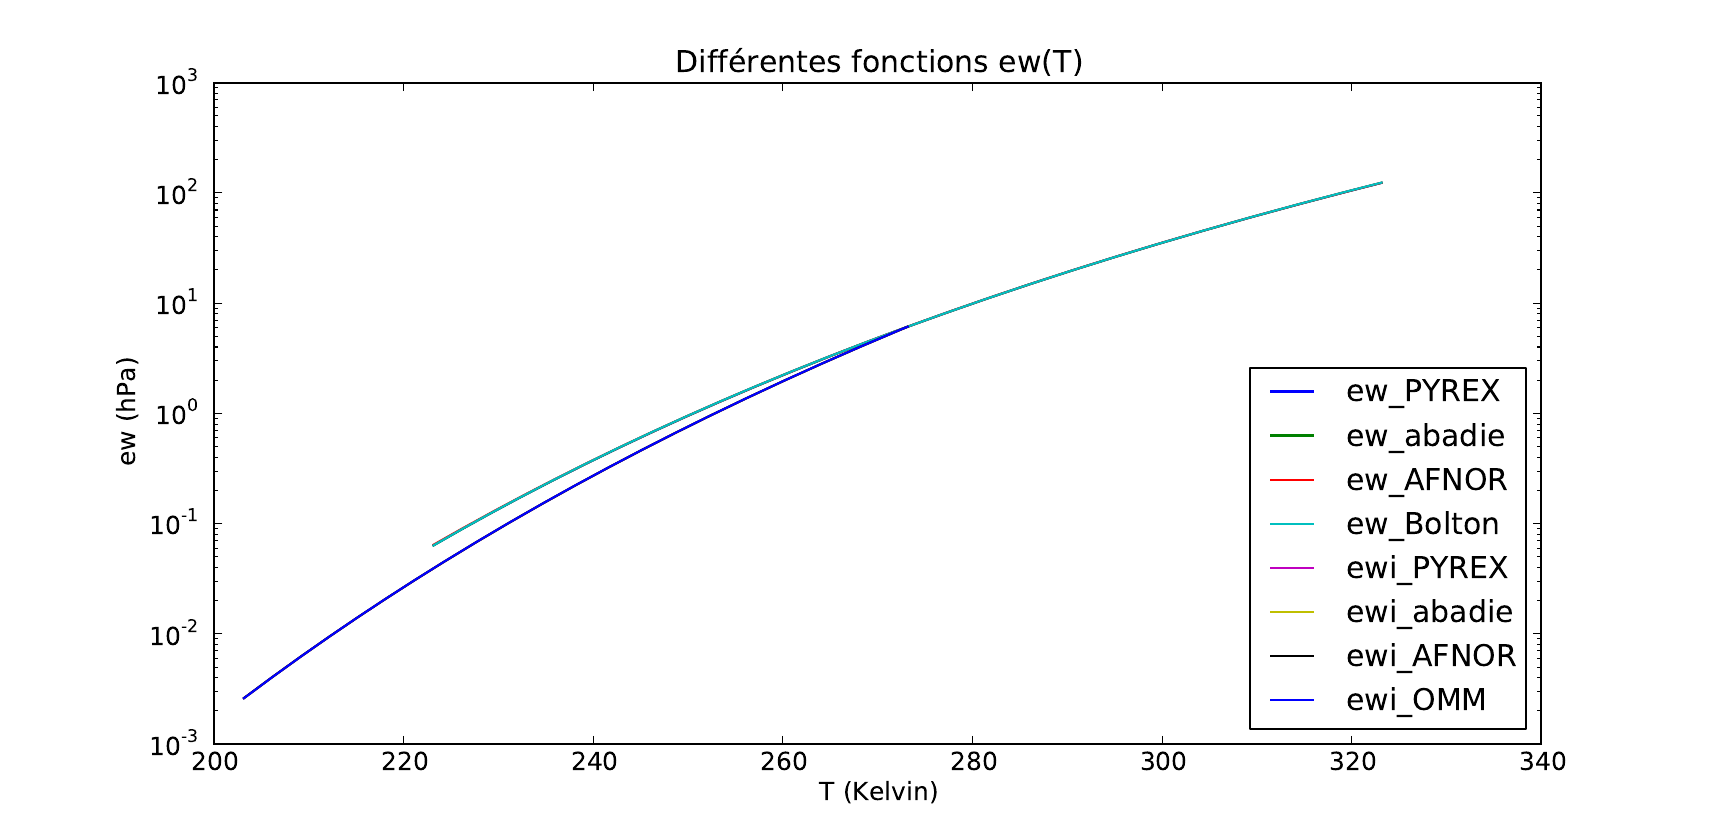
\includegraphics[width=0.99\linewidth]{images/ew_AIDA.png}
\captionof{figure}{Repr�sentation graphique des fonctions ew(T)}
\label{fig-superp_ew}

La figure suivante (\ref{fig-ecart_abs_ew}) pr�sente les trac�s des
�carts entre chaque fonction et la moyenne. Les �carts maxima apparaissent
pour les fortes valeurs de e$_w$, et ne d�passent pas 0.4 hPa.

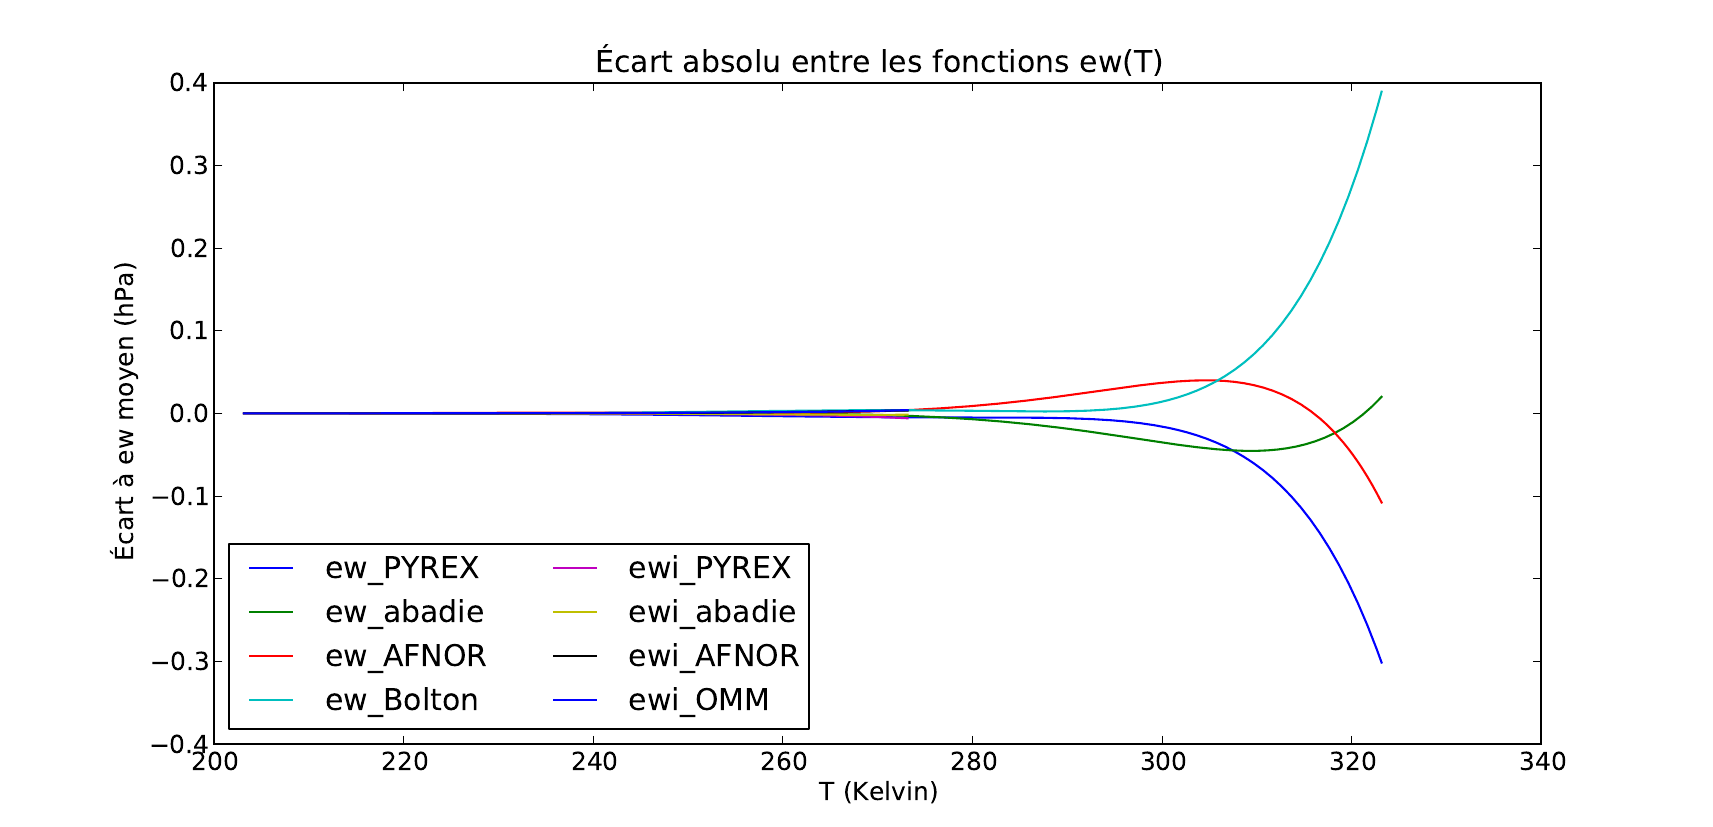
\includegraphics[width=0.99\linewidth]{images/diff-abs-ew-AIDA.png}
\captionof{figure}{�carts absolus}
\label{fig-ecart_abs_ew}

Enfin, le trac� des �carts relatifs (toujours par rapport � la moyenne) 
(figure \ref{fig-ecart_rel_ew}) 
montre que cet �cart est la plupart du temps inf�rieur � 0,3\%,
et ne d�passe jamais 1\%.

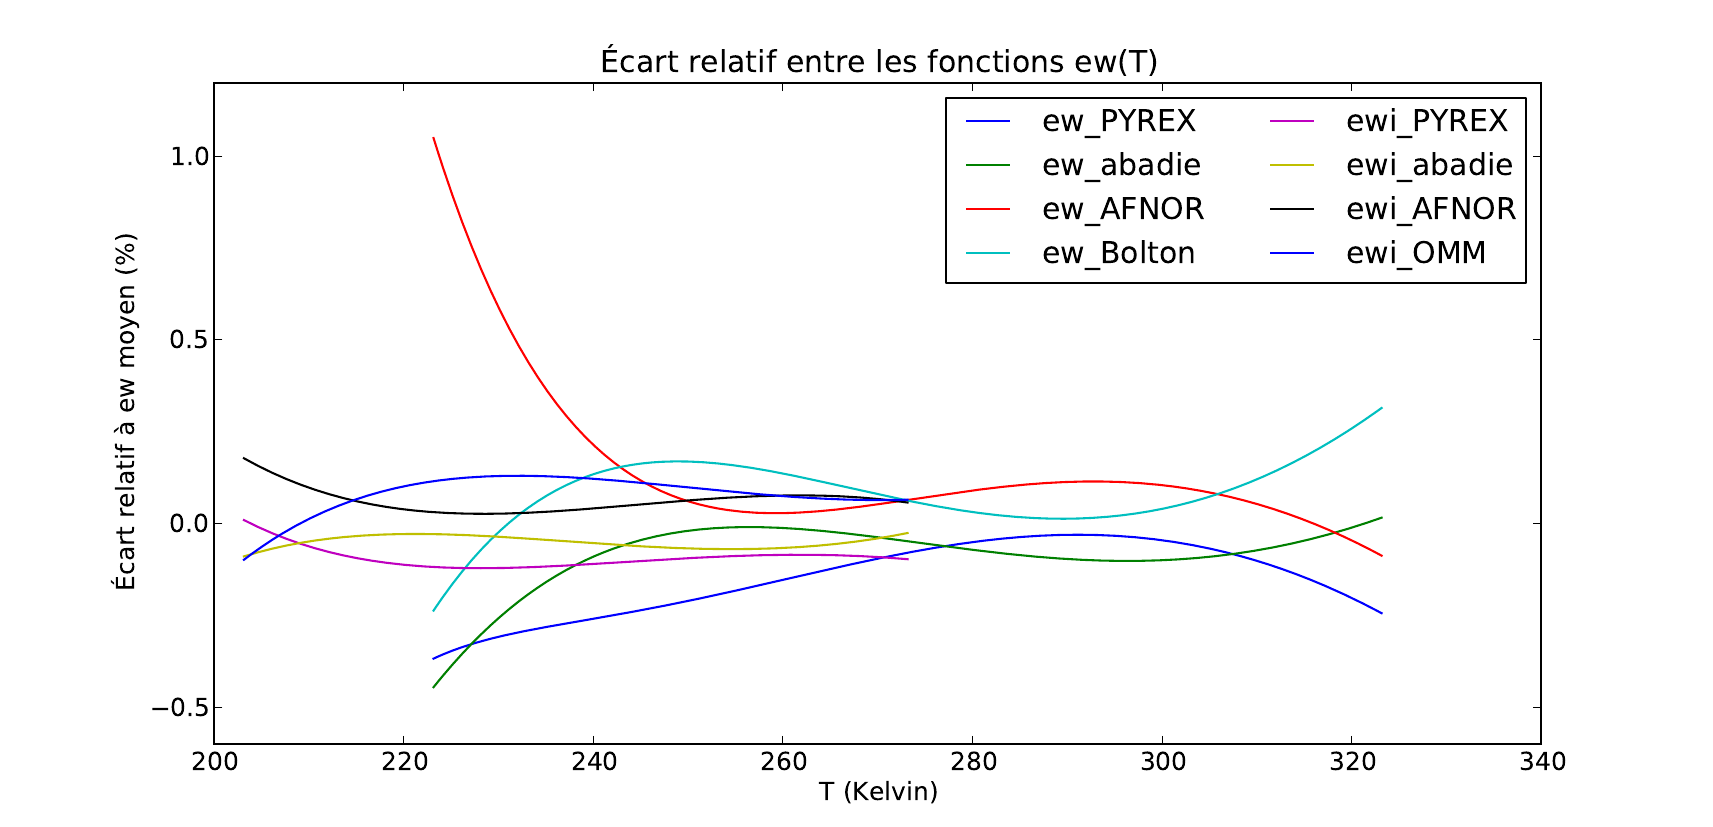
\includegraphics[width=0.99\linewidth]{images/diff-rel-ew-AIDA.png}
\captionof{figure}{�carts relatifs}
\label{fig-ecart_rel_ew}


\newpage
\subsection{Temp�ratures potentielles et potentielles �quivalentes}

\subsubsection{Fonction : \texttt{tpot}}

%%%%%FORMULE%%%%
\itemstyle{Formule}

% Formule d�crivant le calcul fait dans la fonction tpot de la biblioth�que "thermo"
\[
\theta = T_s.\left( \frac{1000}{P_s} \right)^{R_a/c_{pa}}
\]

avec~:\\
$Ts$ : temp�rature, en Kelvin.\\
$Ps$ : pression, en hPa.\\

%%%%%AUTEUR%%%%
\itemstyle{Auteur~:}
CNRM/GMEI/TRAMM

%%%%%REFERENCE%%%%
\itemstyle{R\'ef\'erences~:}
M\'et\'eorologie G\'en\'erale, Triplet-Roche \cite{Triplet-Roche}

\subsubsection{Fonction : \texttt{tpoteq}}

%%%%%FORMULE%%%%
\itemstyle{Formule}

% tpoteq
% calcul de la temp�rature potentielle equivalente 

\[
\theta_e = \theta .\left( 1 + r. \frac{L}{c_{pa}.T_s} \right) 
\]
avec $ L = 3136.17 - 2.34\times T_s $ (pour $T_s$ exprim\'e en $K$).\\


%%%%%AUTEUR%%%%
\itemstyle{Auteur~:}
CNRM/GMEI/TRAMM

%%%%%REFERENCE%%%%
\itemstyle{R\'ef\'erences~:}
Fonction utilis\'ee par Pierre Durand (L.A.).

\subsubsection{Fonction : \texttt{tpot\_Bolton}}

%%%%%FORMULE%%%%
\itemstyle{Formule}

%%tpot_Bolton
% Calcul de la temp�rature potentielle selon la formule de BOLTON
% � partir de Ps, Ts et Hum 

$$
\theta = T_s . \frac{1000}{P_s} ^{ 0.2854 . \left(1-0.00028 . r_{mel}\right) }
$$
avec \\
   $T_s$ : Temp�rature en degr�s Kelvin \\
   $P_s$ : Pression en hPa  \\
   $r_{mel}$ : rapport de m�lange en g/kg .


%%%%%AUTEUR%%%%
\itemstyle{Auteur~:}
CNRM/GMEI/TRAMM

%%%%%REFERENCE%%%%
\itemstyle{R\'ef\'erences~:}
Bolton 1980 \cite{Bolton-80} -Formule 7

\subsubsection{Fonction : \texttt{tpoteq\_Bolton}}

%%%%%FORMULE%%%%
\itemstyle{Formule}

%%tpoteq_Bolton
% Calcul de la temp�rature potentielle �quivalente selon la formule de BOLTON
% � partir de Ps, Ts et Hum 

$$
\theta_e = \theta . \exp \left( \left( \frac{3.376}{T_{cond}} - 0.00254 \right) . r_{mel}. \left( 1 + 0.00081 . r_{mel} \right) \right) 
$$
avec \\
       $\theta$ : Temp�rature potentielle en degr�s Kelvin \\ 
       $T_{cond}$ : Temp�rature du point de condensation en degr�s Kelvin \\
       $r_{mel}$ : rapport de m�lange en g/kg 


%%%%%AUTEUR%%%%
\itemstyle{Auteur~:}
CNRM/GMEI/TRAMM

%%%%%REFERENCE%%%%
\itemstyle{R\'ef\'erences~:}
Bolton 1980 \cite{Bolton-80} -Formule 43

\newpage
\subsection{Transformations adiabatiques et Point de condensation}

Deux fonctions sont utilis�es pour conna\^itre le point de condensation
d'une particule d'air d�finie par $P_s$, $T_s$ et $Hu$ (pression, temp�rature.
et humidit� relative). 
Ces 2 fonctions sont tcond() et pcond() qui permettent respectivement
de calculer la temp�rature et la pression de ce point de condensation.

\subsubsection{Fonction : \texttt{tcond}}

%%%%%FORMULE%%%%
\itemstyle{Formule}

%%% tcond
\[
t_{cond} =  \frac{1}{\frac{1}{T_s-55} - \frac{\ln(Hum/100)}{2840}} + 55
\]


%%%%%AUTEUR%%%%
\itemstyle{Auteur~:}
CNRM/GMEI/TRAMM d'apr�s LIBMTO D. Puech .

%%%%%REFERENCE%%%%
\itemstyle{R\'ef\'erences~:}
Bolton-1980  \cite{Bolton-80}, eq. 22, page 1048.

\subsubsection{Fonction : \texttt{pcond}}

%%%%%FORMULE%%%%
\itemstyle{Formule}

%%% pcond
\[
p_{cond} =  P_s \frac{ew(T_{cond})}{ew(T_s) . \frac{Hum}{100}}
\]


%%%%COMMENTAIRE%%%%
\itemstyle{Commentaire~:}

Le calcul se fait en deux temps :
\begin{itemize}
\item 1 : calcul de $T_{cond}$ par la fonction $tcond()$
\item 2 : calcul de $P_{cond}$ par �galit� du rapport des rapports de 
m�lange entre les 2 niveaux de pression $P_s$ et $P_{cond}$.
\end{itemize}

La fonction $ew()$ utilis�e est celle de l'article de Bolton \cite{Bolton-80}
d�crite ci-dessus au paragraphe \ref{annexe-ewbolton}.

%%%%%AUTEUR%%%%
\itemstyle{Auteur~:}
CNRM/GMEI/TRAMM d'apr�s LIBMTO D. Puech .

%%%%%REFERENCE%%%%
\itemstyle{R\'ef\'erences~:}

\newpage
%%%%
\subsection{Transformations pseudo-adiabatiques}

Calcul d'une temp�rature pseudo-adiabatique pour un niveau de pression donn� 
� partir du point de condensation (temp�rature et pression).

\subsubsection{Fonction : \texttt{twcurv}}

%%%%%FORMULE%%%%
\itemstyle{Formule}

%%% twcurv
La temp�rature $T'_w$ est calcul�e de la fa�on suivante :
\[
rap = \left(\frac{P_{calc}}{P_s - ew_t}\right)^\alpha 
\]
\[
fact = \frac{0.62198}{C_p . P_{calc}} 
\]
\[
\rho_p = \frac{0.62198 . Clw\left(t\right) . ew_t . P_s}{C_p . T_s} 
\]
It�ration jusqu'� la convergence entre la temp�rature $y$ et la temp�rature $x$.\newline
La temp�rature $x$ est initialis�e � $T_s$ avant la boucle. \\
D�but de la boucle de calcul it�ratif : \\
\[
de = \left(r_1 + x . \left(r_2 + x . \left(r_3 + x . \left(r_4 + x . \left(r_5 + x. \left(r_6 - x . r_7\right)\right)\right)\right)\right)\right)
\]
\[
x_{kelvin} = x + T_0
\]
\[
a = T_s . rap . \left(1 - \frac{ew_x}{P_{calc}}\right) 
\]
\[
b = \exp{ \frac{\left(\rho_p - Clw\left(x\right)\right) . fact . ew_x}{x_{kelvin}}} 
\]
\[
y = \left(a . b\right) - T_0 
\]
Test de convergence :  \newline
Si la diff�rence entre $x$ et $y$ est inf�rieure � 0.05 (convergence), alors : 
\[
t'_w = y + T_0 
\]
Sinon : 
\[
dydx = a . b . \left( -\alpha . \frac{de}{\left(P_{calc}-ew_x\right)} 
 + fact . Clw\left(x\right) . \frac{\left(\frac{ew_x}{x_{kelvin}}
 - de\right)}{xk}\right) 
\]
\[
x = \frac{\left( y - x . dydx\right)}{\left(1. - dydx\right)} 
\]
Fin de boucle

avec~:\newline
$P_s = $ Pression du niveau de condensation en hPa \newline
$T_s = $ Temp�rature du niveau de condensation en degres Celsius \newline
$P_{calc} = $ Pression du niveau de calcul en hPa \\
$ew_t = $ Tension de vapeur partielle, calcul� par la formule
 donn�e dans Bolton-80.  \\
$\alpha = \frac{R_a}{C_{pa}} = 0.28562 $ \\
$C_p = 1005. $ \\
$r_1 = 4.438099984e^{-1} $ \\
$r_2 = 2.857002636e^{-2} $ \\
$r_3 = 7.938054040e^{-4} $ \\
$r_4 = 1.215215065e^{-6} $ \\
$r_5 = 1.036561403e^{-7} $ \\
$r_6 = 3.532421810e^{-10} $ \\
$r_7 = 7.090244484e^{-13} $ \\
$T_0 = 273.15 $ \\


%%%%%AUTEUR%%%%
\itemstyle{Auteur~:}
CNRM/GMEI/TRAMM d'apr�s LIBMTO D. Puech .

%%%%%REFERENCE%%%%
\itemstyle{R\'ef\'erences~:}

\newpage
%%%%
\subsection{Utilisation de la temp�rature virtuelle}

calcul de la masse volumique d'une particule d'air humide
d�finie par : pression , temp�rature , humidit� .

\subsubsection{Fonction : \texttt{DensAirhum}}

%%%%%FORMULE%%%%
\itemstyle{Formule}

%% calcul de la densite de l'air humide
$$
Dens = \frac{P_s\times 100}{R_a \times T_v}
$$
avec $R_a = 287.05 J.kg^{-1}.K^{-1} $, et $T_v$ exprim\'e 
en $K$.


%%%%%AUTEUR%%%%
\itemstyle{Auteur~:}
CNRM/GMEI/TRAMM d'apr�s LIBMTO D. Puech .

%%%%%REFERENCE%%%%
\itemstyle{R\'ef\'erences~:}

\subsubsection{Fonction : \texttt{TVirt\_ptu}}

%%%%%FORMULE%%%%
\itemstyle{Formule}

%%%% Tempe virtuelle calcul�e avec Ps, Ts, Hum
\[
e_w = r_1^{ \left( \displaystyle
                \frac{r_2 . T_s}{T_s + r_3}
                \right) }
e = Hum . e_w/r_4
r = frac{r_5 . e}{P_s - e}
TVirt = frac{(1 + r_7 . r) . (T_s + T_0)}{1 + r} - r_7
\]
avec~:\\
$r_1 = 6.112 $ \\
$r_2 = 17.67 $ \\
$r_3 = 243.5 $\\
$r_4 = 100.  $\\
$r_4 = .622  $\\
$r_6 = 1000.  $\\
$T_0 = 273.15  $\\
$r_7 = 1.608  $\\


%%%%%AUTEUR%%%%
\itemstyle{Auteur~:}
CNRM/GMEI/TRAMM d'apr�s LIBMTO D. Puech .

%%%%%REFERENCE%%%%
\itemstyle{R\'ef\'erences~:}

%%%%%%%
%
\section{Traitement du signal}
\label{annexe-traitsign}

\subsection{FFT}

%%\chapter{D�finitions}
%%%%%%%
%
\label{annexe-definitions}
\section{Thermodynamique Atmosph�rique}
\subsection{humidit� sp�cifique}
\subsection{rapport de m�lange}
\subsection{humidit� absolue}
\subsection{humidit� relative}




%%% BIBLIO
\bibliographystyle{plain}
%%\bibliographystyle{frplain}
\bibliography{oper}

%%% INDEX
\clearpage
\newpage
% probl�me de r�f�rence de la page index...
\phantomsection
\printindex
\end{document}
